\documentclass[twoside]{book}

% Packages required by doxygen
\usepackage{fixltx2e}
\usepackage{calc}
\usepackage{doxygen}
\usepackage[export]{adjustbox} % also loads graphicx
\usepackage{graphicx}
\usepackage[utf8]{inputenc}
\usepackage{makeidx}
\usepackage{multicol}
\usepackage{multirow}
\PassOptionsToPackage{warn}{textcomp}
\usepackage{textcomp}
\usepackage[nointegrals]{wasysym}
\usepackage[table]{xcolor}

% Font selection
\usepackage[T1]{fontenc}
\usepackage[scaled=.90]{helvet}
\usepackage{courier}
\usepackage{amssymb}
\usepackage{sectsty}
\renewcommand{\familydefault}{\sfdefault}
\allsectionsfont{%
  \fontseries{bc}\selectfont%
  \color{darkgray}%
}
\renewcommand{\DoxyLabelFont}{%
  \fontseries{bc}\selectfont%
  \color{darkgray}%
}
\newcommand{\+}{\discretionary{\mbox{\scriptsize$\hookleftarrow$}}{}{}}

% Page & text layout
\usepackage{geometry}
\geometry{%
  a4paper,%
  top=2.5cm,%
  bottom=2.5cm,%
  left=2.5cm,%
  right=2.5cm%
}
\tolerance=750
\hfuzz=15pt
\hbadness=750
\setlength{\emergencystretch}{15pt}
\setlength{\parindent}{0cm}
\setlength{\parskip}{3ex plus 2ex minus 2ex}
\makeatletter
\renewcommand{\paragraph}{%
  \@startsection{paragraph}{4}{0ex}{-1.0ex}{1.0ex}{%
    \normalfont\normalsize\bfseries\SS@parafont%
  }%
}
\renewcommand{\subparagraph}{%
  \@startsection{subparagraph}{5}{0ex}{-1.0ex}{1.0ex}{%
    \normalfont\normalsize\bfseries\SS@subparafont%
  }%
}
\makeatother

% Headers & footers
\usepackage{fancyhdr}
\pagestyle{fancyplain}
\fancyhead[LE]{\fancyplain{}{\bfseries\thepage}}
\fancyhead[CE]{\fancyplain{}{}}
\fancyhead[RE]{\fancyplain{}{\bfseries\leftmark}}
\fancyhead[LO]{\fancyplain{}{\bfseries\rightmark}}
\fancyhead[CO]{\fancyplain{}{}}
\fancyhead[RO]{\fancyplain{}{\bfseries\thepage}}
\fancyfoot[LE]{\fancyplain{}{}}
\fancyfoot[CE]{\fancyplain{}{}}
\fancyfoot[RE]{\fancyplain{}{\bfseries\scriptsize Generated by Doxygen }}
\fancyfoot[LO]{\fancyplain{}{\bfseries\scriptsize Generated by Doxygen }}
\fancyfoot[CO]{\fancyplain{}{}}
\fancyfoot[RO]{\fancyplain{}{}}
\renewcommand{\footrulewidth}{0.4pt}
\renewcommand{\chaptermark}[1]{%
  \markboth{#1}{}%
}
\renewcommand{\sectionmark}[1]{%
  \markright{\thesection\ #1}%
}

% Indices & bibliography
\usepackage{natbib}
\usepackage[titles]{tocloft}
\setcounter{tocdepth}{3}
\setcounter{secnumdepth}{5}
\makeindex

% Hyperlinks (required, but should be loaded last)
\usepackage{ifpdf}
\ifpdf
  \usepackage[pdftex,pagebackref=true]{hyperref}
\else
  \usepackage[ps2pdf,pagebackref=true]{hyperref}
\fi
\hypersetup{%
  colorlinks=true,%
  linkcolor=blue,%
  citecolor=blue,%
  unicode%
}

% Custom commands
\newcommand{\clearemptydoublepage}{%
  \newpage{\pagestyle{empty}\cleardoublepage}%
}

\usepackage{caption}
\captionsetup{labelsep=space,justification=centering,font={bf},singlelinecheck=off,skip=4pt,position=top}

%===== C O N T E N T S =====

\begin{document}

% Titlepage & ToC
\hypersetup{pageanchor=false,
             bookmarksnumbered=true,
             pdfencoding=unicode
            }
\pagenumbering{alph}
\begin{titlepage}
\vspace*{7cm}
\begin{center}%
{\Large My Project }\\
\vspace*{1cm}
{\large Generated by Doxygen 1.8.13}\\
\end{center}
\end{titlepage}
\clearemptydoublepage
\pagenumbering{roman}
\tableofcontents
\clearemptydoublepage
\pagenumbering{arabic}
\hypersetup{pageanchor=true}

%--- Begin generated contents ---
\chapter{Hierarchical Index}
\section{Class Hierarchy}
This inheritance list is sorted roughly, but not completely, alphabetically\+:\begin{DoxyCompactList}
\item \contentsline{section}{biogeme.\+B\+I\+O\+G\+E\+M\+E\+\_\+\+O\+B\+J\+E\+CT}{\pageref{classbiogeme_1_1_b_i_o_g_e_m_e___o_b_j_e_c_t}}{}
\item \contentsline{section}{bio\+\_\+expression.\+Expression}{\pageref{classbio__expression_1_1_expression}}{}
\begin{DoxyCompactList}
\item \contentsline{section}{bio\+\_\+expression.\+abs}{\pageref{classbio__expression_1_1abs}}{}
\item \contentsline{section}{bio\+\_\+expression.\+Beta}{\pageref{classbio__expression_1_1_beta}}{}
\item \contentsline{section}{bio\+\_\+expression.\+Bin\+Op}{\pageref{classbio__expression_1_1_bin_op}}{}
\item \contentsline{section}{bio\+\_\+expression.\+bio\+Bayes\+Normal\+Draw}{\pageref{classbio__expression_1_1bio_bayes_normal_draw}}{}
\item \contentsline{section}{bio\+\_\+expression.\+bio\+Draws}{\pageref{classbio__expression_1_1bio_draws}}{}
\item \contentsline{section}{bio\+\_\+expression.\+bio\+Logit}{\pageref{classbio__expression_1_1bio_logit}}{}
\item \contentsline{section}{bio\+\_\+expression.\+bio\+Log\+Logit}{\pageref{classbio__expression_1_1bio_log_logit}}{}
\item \contentsline{section}{bio\+\_\+expression.\+bio\+Mult\+Sum}{\pageref{classbio__expression_1_1bio_mult_sum}}{}
\item \contentsline{section}{bio\+\_\+expression.\+bio\+Normal\+Cdf}{\pageref{classbio__expression_1_1bio_normal_cdf}}{}
\item \contentsline{section}{bio\+\_\+expression.\+bio\+Normal\+Draws}{\pageref{classbio__expression_1_1bio_normal_draws}}{}
\item \contentsline{section}{bio\+\_\+expression.\+bio\+Normal\+Pdf}{\pageref{classbio__expression_1_1bio_normal_pdf}}{}
\item \contentsline{section}{bio\+\_\+expression.\+bio\+Recycle\+Draws}{\pageref{classbio__expression_1_1bio_recycle_draws}}{}
\item \contentsline{section}{bio\+\_\+expression.\+bio\+Uniform\+Draws}{\pageref{classbio__expression_1_1bio_uniform_draws}}{}
\item \contentsline{section}{bio\+\_\+expression.\+bio\+Uniform\+Symmetric\+Draws}{\pageref{classbio__expression_1_1bio_uniform_symmetric_draws}}{}
\item \contentsline{section}{bio\+\_\+expression.\+Define\+Draws}{\pageref{classbio__expression_1_1_define_draws}}{}
\item \contentsline{section}{bio\+\_\+expression.\+Define\+Variable}{\pageref{classbio__expression_1_1_define_variable}}{}
\item \contentsline{section}{bio\+\_\+expression.\+Derive}{\pageref{classbio__expression_1_1_derive}}{}
\item \contentsline{section}{bio\+\_\+expression.\+Elem}{\pageref{classbio__expression_1_1_elem}}{}
\item \contentsline{section}{bio\+\_\+expression.\+Enumerate}{\pageref{classbio__expression_1_1_enumerate}}{}
\item \contentsline{section}{bio\+\_\+expression.\+exp}{\pageref{classbio__expression_1_1exp}}{}
\item \contentsline{section}{bio\+\_\+expression.\+Integrate}{\pageref{classbio__expression_1_1_integrate}}{}
\item \contentsline{section}{bio\+\_\+expression.\+log}{\pageref{classbio__expression_1_1log}}{}
\item \contentsline{section}{bio\+\_\+expression.\+max}{\pageref{classbio__expression_1_1max}}{}
\item \contentsline{section}{bio\+\_\+expression.\+MH}{\pageref{classbio__expression_1_1_m_h}}{}
\item \contentsline{section}{bio\+\_\+expression.\+min}{\pageref{classbio__expression_1_1min}}{}
\item \contentsline{section}{bio\+\_\+expression.\+Monte\+Carlo}{\pageref{classbio__expression_1_1_monte_carlo}}{}
\item \contentsline{section}{bio\+\_\+expression.\+Monte\+Carlo\+Control\+Variate}{\pageref{classbio__expression_1_1_monte_carlo_control_variate}}{}
\item \contentsline{section}{bio\+\_\+expression.\+Numeric}{\pageref{classbio__expression_1_1_numeric}}{}
\item \contentsline{section}{bio\+\_\+expression.\+Prod}{\pageref{classbio__expression_1_1_prod}}{}
\item \contentsline{section}{bio\+\_\+expression.\+Random\+Variable}{\pageref{classbio__expression_1_1_random_variable}}{}
\item \contentsline{section}{bio\+\_\+expression.\+Sum}{\pageref{classbio__expression_1_1_sum}}{}
\item \contentsline{section}{bio\+\_\+expression.\+Un\+Op}{\pageref{classbio__expression_1_1_un_op}}{}
\item \contentsline{section}{bio\+\_\+expression.\+Variable}{\pageref{classbio__expression_1_1_variable}}{}
\end{DoxyCompactList}
\item \contentsline{section}{bio\+\_\+iterator.\+iterator}{\pageref{classbio__iterator_1_1iterator}}{}
\begin{DoxyCompactList}
\item \contentsline{section}{bio\+\_\+iterator.\+draw\+Iterator}{\pageref{classbio__iterator_1_1draw_iterator}}{}
\item \contentsline{section}{bio\+\_\+iterator.\+meta\+Iterator}{\pageref{classbio__iterator_1_1meta_iterator}}{}
\item \contentsline{section}{bio\+\_\+iterator.\+row\+Iterator}{\pageref{classbio__iterator_1_1row_iterator}}{}
\end{DoxyCompactList}
\item object\begin{DoxyCompactList}
\item \contentsline{section}{bio\+Matrix.\+bio\+Matrix}{\pageref{classbio_matrix_1_1bio_matrix}}{}
\end{DoxyCompactList}
\item \contentsline{section}{bio\+\_\+expression.\+Operator}{\pageref{classbio__expression_1_1_operator}}{}
\item \contentsline{section}{biogeme.\+S\+T\+AN}{\pageref{classbiogeme_1_1_s_t_a_n}}{}
\end{DoxyCompactList}

\chapter{Class Index}
\section{Class List}
Here are the classes, structs, unions and interfaces with brief descriptions\+:\begin{DoxyCompactList}
\item\contentsline{section}{\hyperlink{classbio__expression_1_1abs}{bio\+\_\+expression.\+abs} \\*Class representing the expression for absolute value }{\pageref{classbio__expression_1_1abs}}{}
\item\contentsline{section}{\hyperlink{classbio__expression_1_1_beta}{bio\+\_\+expression.\+Beta} \\*Class representing a parameter to be estimated }{\pageref{classbio__expression_1_1_beta}}{}
\item\contentsline{section}{\hyperlink{classbio__expression_1_1_bin_op}{bio\+\_\+expression.\+Bin\+Op} \\*Generic class for binary operators }{\pageref{classbio__expression_1_1_bin_op}}{}
\item\contentsline{section}{\hyperlink{classbio__expression_1_1bio_bayes_normal_draw}{bio\+\_\+expression.\+bio\+Bayes\+Normal\+Draw} \\*Class performing draws from the posterior of the mean of a normal variable knowing realizations and variance }{\pageref{classbio__expression_1_1bio_bayes_normal_draw}}{}
\item\contentsline{section}{\hyperlink{classbio__expression_1_1bio_draws}{bio\+\_\+expression.\+bio\+Draws} \\*Class representing a random variable for integration using Monte Carlo simulation }{\pageref{classbio__expression_1_1bio_draws}}{}
\item\contentsline{section}{\hyperlink{classbiogeme_1_1_b_i_o_g_e_m_e___o_b_j_e_c_t}{biogeme.\+B\+I\+O\+G\+E\+M\+E\+\_\+\+O\+B\+J\+E\+CT} \\*This class gathers the components needed by biogeme to perform the estimation or the simulation }{\pageref{classbiogeme_1_1_b_i_o_g_e_m_e___o_b_j_e_c_t}}{}
\item\contentsline{section}{\hyperlink{classbio__expression_1_1bio_logit}{bio\+\_\+expression.\+bio\+Logit} \\*Class calculating a logit choice probability }{\pageref{classbio__expression_1_1bio_logit}}{}
\item\contentsline{section}{\hyperlink{classbio__expression_1_1bio_log_logit}{bio\+\_\+expression.\+bio\+Log\+Logit} \\*Class calculating the log of a logit choice probability }{\pageref{classbio__expression_1_1bio_log_logit}}{}
\item\contentsline{section}{\hyperlink{classbio_matrix_1_1bio_matrix}{bio\+Matrix.\+bio\+Matrix} \\*This class implements a matrix object designed to store the variance covariance matrix }{\pageref{classbio_matrix_1_1bio_matrix}}{}
\item\contentsline{section}{\hyperlink{classbio__expression_1_1bio_mult_sum}{bio\+\_\+expression.\+bio\+Mult\+Sum} \\*Class computing the sum of multiple expressions }{\pageref{classbio__expression_1_1bio_mult_sum}}{}
\item\contentsline{section}{\hyperlink{classbio__expression_1_1bio_normal_cdf}{bio\+\_\+expression.\+bio\+Normal\+Cdf} \\*Class representing the cumulative distribution function of the normal distribution }{\pageref{classbio__expression_1_1bio_normal_cdf}}{}
\item\contentsline{section}{\hyperlink{classbio__expression_1_1bio_normal_draws}{bio\+\_\+expression.\+bio\+Normal\+Draws} \\*Class representing a normally distributed random variable for simulated integration }{\pageref{classbio__expression_1_1bio_normal_draws}}{}
\item\contentsline{section}{\hyperlink{classbio__expression_1_1bio_normal_pdf}{bio\+\_\+expression.\+bio\+Normal\+Pdf} \\*Class representing the probability density function of a standardized normally distributed random variable }{\pageref{classbio__expression_1_1bio_normal_pdf}}{}
\item\contentsline{section}{\hyperlink{classbio__expression_1_1bio_recycle_draws}{bio\+\_\+expression.\+bio\+Recycle\+Draws} \\*Class representing the uniform draw of a random variable used for integration using Monte Carlo simulation }{\pageref{classbio__expression_1_1bio_recycle_draws}}{}
\item\contentsline{section}{\hyperlink{classbio__expression_1_1bio_uniform_draws}{bio\+\_\+expression.\+bio\+Uniform\+Draws} \\*Class representing a uniformly distributed random variable on \mbox{[}0,1\mbox{]} for simulated integration }{\pageref{classbio__expression_1_1bio_uniform_draws}}{}
\item\contentsline{section}{\hyperlink{classbio__expression_1_1bio_uniform_symmetric_draws}{bio\+\_\+expression.\+bio\+Uniform\+Symmetric\+Draws} \\*Class representing a uniformly distributed random variable on \mbox{[}-\/1,1\mbox{]} for simulated integration }{\pageref{classbio__expression_1_1bio_uniform_symmetric_draws}}{}
\item\contentsline{section}{\hyperlink{classbio__expression_1_1_define_draws}{bio\+\_\+expression.\+Define\+Draws} \\*Class representing the definition of a new type of draws }{\pageref{classbio__expression_1_1_define_draws}}{}
\item\contentsline{section}{\hyperlink{classbio__expression_1_1_define_variable}{bio\+\_\+expression.\+Define\+Variable} \\*Class representing the definition of a new variable }{\pageref{classbio__expression_1_1_define_variable}}{}
\item\contentsline{section}{\hyperlink{classbio__expression_1_1_derive}{bio\+\_\+expression.\+Derive} \\*Class generating the analytical derivative of an expression }{\pageref{classbio__expression_1_1_derive}}{}
\item\contentsline{section}{\hyperlink{classbio__iterator_1_1draw_iterator}{bio\+\_\+iterator.\+draw\+Iterator} \\*Iterates on the data file for generate the user defined draws (since biogeme 2.\+4) }{\pageref{classbio__iterator_1_1draw_iterator}}{}
\item\contentsline{section}{\hyperlink{classbio__expression_1_1_elem}{bio\+\_\+expression.\+Elem} \\*Class extracting an expression from a dictionary }{\pageref{classbio__expression_1_1_elem}}{}
\item\contentsline{section}{\hyperlink{classbio__expression_1_1_enumerate}{bio\+\_\+expression.\+Enumerate} \\*Class performing a sample enumeration }{\pageref{classbio__expression_1_1_enumerate}}{}
\item\contentsline{section}{\hyperlink{classbio__expression_1_1exp}{bio\+\_\+expression.\+exp} \\*Class representing the expression for exponential }{\pageref{classbio__expression_1_1exp}}{}
\item\contentsline{section}{\hyperlink{classbio__expression_1_1_expression}{bio\+\_\+expression.\+Expression} \\*Interface for mathematical expressions }{\pageref{classbio__expression_1_1_expression}}{}
\item\contentsline{section}{\hyperlink{classbio__expression_1_1_integrate}{bio\+\_\+expression.\+Integrate} \\*Class performing numerical integration relying on the \href{http://en.wikipedia.org/wiki/Gaussian_quadrature}{\tt Gauss-\/\+Hermite quadrature} to compute \[ \int_{-\infty}^{+\infty} f(\omega) d\omega. \] }{\pageref{classbio__expression_1_1_integrate}}{}
\item\contentsline{section}{\hyperlink{classbio__iterator_1_1iterator}{bio\+\_\+iterator.\+iterator} \\*Generic class for an iterator }{\pageref{classbio__iterator_1_1iterator}}{}
\item\contentsline{section}{\hyperlink{classbio__expression_1_1log}{bio\+\_\+expression.\+log} \\*Class representing the expression for natural logarithm }{\pageref{classbio__expression_1_1log}}{}
\item\contentsline{section}{\hyperlink{classbio__expression_1_1max}{bio\+\_\+expression.\+max} \\*Class representing the expression for the maximum of two expressions }{\pageref{classbio__expression_1_1max}}{}
\item\contentsline{section}{\hyperlink{classbio__iterator_1_1meta_iterator}{bio\+\_\+iterator.\+meta\+Iterator} \\*Meta iterators are designed to iterate on group of rows of the data file }{\pageref{classbio__iterator_1_1meta_iterator}}{}
\item\contentsline{section}{\hyperlink{classbio__expression_1_1_m_h}{bio\+\_\+expression.\+MH} \\*Class performing draws from densities for Bayesian estimation using Metropolis-\/\+Hastings algorithm }{\pageref{classbio__expression_1_1_m_h}}{}
\item\contentsline{section}{\hyperlink{classbio__expression_1_1min}{bio\+\_\+expression.\+min} \\*Class representing the expression for the minimum of two expressions }{\pageref{classbio__expression_1_1min}}{}
\item\contentsline{section}{\hyperlink{classbio__expression_1_1_monte_carlo}{bio\+\_\+expression.\+Monte\+Carlo} \\*Class representing the Monte Carlo integration of an expression }{\pageref{classbio__expression_1_1_monte_carlo}}{}
\item\contentsline{section}{\hyperlink{classbio__expression_1_1_monte_carlo_control_variate}{bio\+\_\+expression.\+Monte\+Carlo\+Control\+Variate} \\*Class representing the Monte Carlo integration of an expression, using a control variate method to decrease the variance }{\pageref{classbio__expression_1_1_monte_carlo_control_variate}}{}
\item\contentsline{section}{\hyperlink{classbio__expression_1_1_numeric}{bio\+\_\+expression.\+Numeric} \\*Class wrapping an integer or a float value }{\pageref{classbio__expression_1_1_numeric}}{}
\item\contentsline{section}{\hyperlink{classbio__expression_1_1_operator}{bio\+\_\+expression.\+Operator} \\*Generic class for an operator }{\pageref{classbio__expression_1_1_operator}}{}
\item\contentsline{section}{\hyperlink{classbio__expression_1_1_prod}{bio\+\_\+expression.\+Prod} \\*Class representing the product of the same expression applied to a list of data }{\pageref{classbio__expression_1_1_prod}}{}
\item\contentsline{section}{\hyperlink{classbio__expression_1_1_random_variable}{bio\+\_\+expression.\+Random\+Variable} \\*Class representing a random variable for numerical integration }{\pageref{classbio__expression_1_1_random_variable}}{}
\item\contentsline{section}{\hyperlink{classbio__iterator_1_1row_iterator}{bio\+\_\+iterator.\+row\+Iterator} \\*Row iterators are designed to iterate on rows of the data file }{\pageref{classbio__iterator_1_1row_iterator}}{}
\item\contentsline{section}{\hyperlink{classbiogeme_1_1_s_t_a_n}{biogeme.\+S\+T\+AN} \\*Class used for generating \hyperlink{classbiogeme_1_1_s_t_a_n}{S\+T\+AN} files (see \href{http://mc-stan.org}{\tt http\+://mc-\/stan.\+org}) }{\pageref{classbiogeme_1_1_s_t_a_n}}{}
\item\contentsline{section}{\hyperlink{classbio__expression_1_1_sum}{bio\+\_\+expression.\+Sum} \\*Class representing the sum of the same expression applied to a list of data }{\pageref{classbio__expression_1_1_sum}}{}
\item\contentsline{section}{\hyperlink{classbio__expression_1_1_un_op}{bio\+\_\+expression.\+Un\+Op} \\*Generic class for unary operators }{\pageref{classbio__expression_1_1_un_op}}{}
\item\contentsline{section}{\hyperlink{classbio__expression_1_1_variable}{bio\+\_\+expression.\+Variable} \\*Class representing the variables defined in the data file }{\pageref{classbio__expression_1_1_variable}}{}
\end{DoxyCompactList}

\chapter{Class Documentation}
\hypertarget{class____iterator__panel_obs_iter}{}\section{\+\_\+\+\_\+iterator\+\_\+panel\+Obs\+Iter Class Reference}
\label{class____iterator__panel_obs_iter}\index{\+\_\+\+\_\+iterator\+\_\+panel\+Obs\+Iter@{\+\_\+\+\_\+iterator\+\_\+panel\+Obs\+Iter}}
Inheritance diagram for \+\_\+\+\_\+iterator\+\_\+panel\+Obs\+Iter\+:\begin{figure}[H]
\begin{center}
\leavevmode
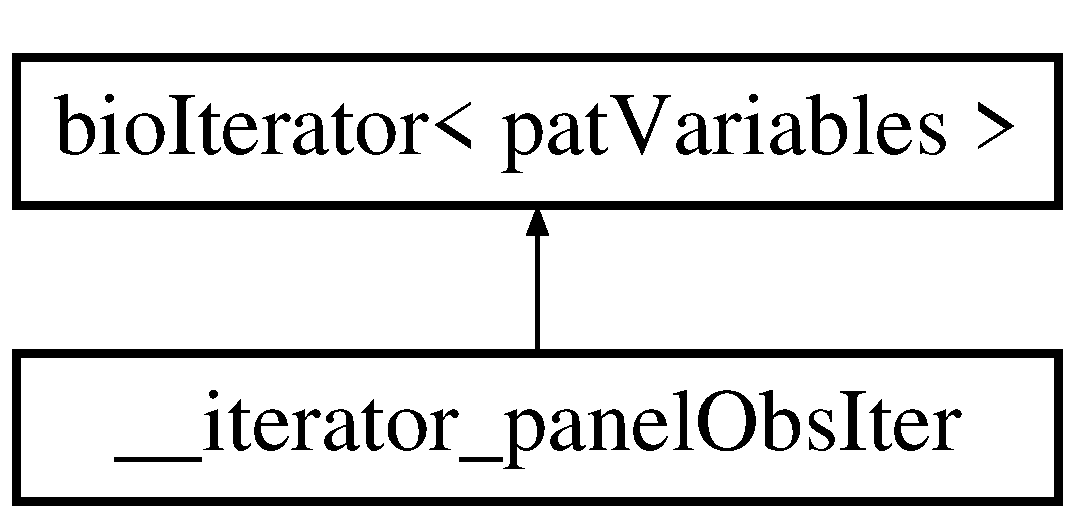
\includegraphics[height=2.000000cm]{class____iterator__panel_obs_iter}
\end{center}
\end{figure}
\subsection*{Protected Attributes}
\begin{DoxyCompactItemize}
\item 
\mbox{\Hypertarget{class____iterator__panel_obs_iter_abb71e1ec5783f7fecc015a66c02b162a}\label{class____iterator__panel_obs_iter_abb71e1ec5783f7fecc015a66c02b162a}} 
pat\+U\+Long {\bfseries first\+Row}
\item 
\mbox{\Hypertarget{class____iterator__panel_obs_iter_a77c38ce5aeaf88a848b93b9770458b41}\label{class____iterator__panel_obs_iter_a77c38ce5aeaf88a848b93b9770458b41}} 
pat\+U\+Long {\bfseries the\+Index}
\item 
\mbox{\Hypertarget{class____iterator__panel_obs_iter_a49b4455cdd4b026545a8e6995a9443e5}\label{class____iterator__panel_obs_iter_a49b4455cdd4b026545a8e6995a9443e5}} 
pat\+Real {\bfseries the\+Test\+Value}
\item 
\mbox{\Hypertarget{class____iterator__panel_obs_iter_ad0e6ecb8c804b9d7334be78a1f6ff29e}\label{class____iterator__panel_obs_iter_ad0e6ecb8c804b9d7334be78a1f6ff29e}} 
pat\+Variables $\ast$ {\bfseries the\+Current\+Row}
\item 
\mbox{\Hypertarget{class____iterator__panel_obs_iter_a1da7a17cc69e689b94c44668c158276c}\label{class____iterator__panel_obs_iter_a1da7a17cc69e689b94c44668c158276c}} 
\hyperlink{classbio_sample}{bio\+Sample} $\ast$ {\bfseries the\+Sample}
\item 
\mbox{\Hypertarget{class____iterator__panel_obs_iter_a55c10be3d713f12284fdcd7a524b48f3}\label{class____iterator__panel_obs_iter_a55c10be3d713f12284fdcd7a524b48f3}} 
pat\+U\+Long {\bfseries current\+Row\+Index}
\end{DoxyCompactItemize}
\subsection*{Additional Inherited Members}


The documentation for this class was generated from the following files\+:\begin{DoxyCompactItemize}
\item 
\+\_\+\+\_\+iterator\+\_\+panel\+Obs\+Iter.\+h\item 
\+\_\+\+\_\+iterator\+\_\+panel\+Obs.\+cc\end{DoxyCompactItemize}

\hypertarget{classbio_arith_abs}{}\section{bio\+Arith\+Abs Class Reference}
\label{classbio_arith_abs}\index{bio\+Arith\+Abs@{bio\+Arith\+Abs}}


{\ttfamily \#include $<$bio\+Arith\+Abs.\+h$>$}

Inheritance diagram for bio\+Arith\+Abs\+:\begin{figure}[H]
\begin{center}
\leavevmode
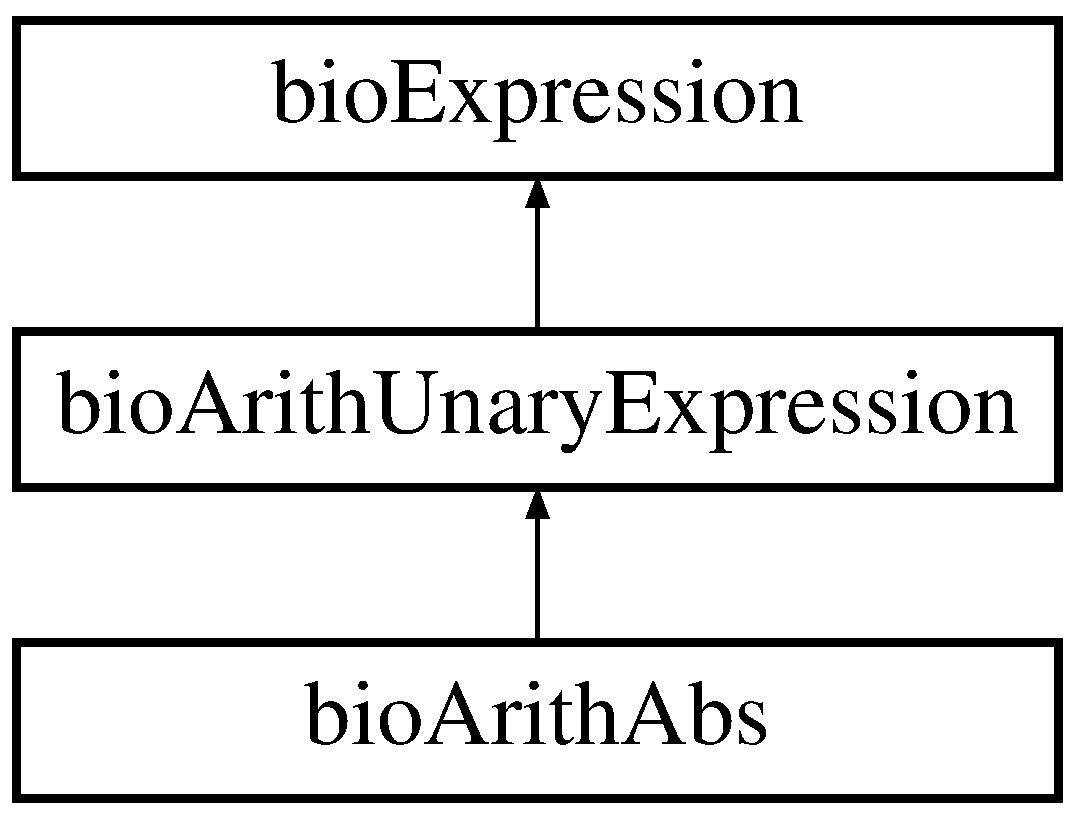
\includegraphics[height=3.000000cm]{classbio_arith_abs}
\end{center}
\end{figure}
\subsection*{Public Member Functions}
\begin{DoxyCompactItemize}
\item 
\mbox{\Hypertarget{classbio_arith_abs_a8c92472b2d9e4abbb84894383e06513f}\label{classbio_arith_abs_a8c92472b2d9e4abbb84894383e06513f}} 
{\bfseries bio\+Arith\+Abs} (\hyperlink{classbio_expression_repository}{bio\+Expression\+Repository} $\ast$rep, pat\+U\+Long par, pat\+U\+Long c, pat\+Error $\ast$\&err)
\item 
virtual pat\+String \hyperlink{classbio_arith_abs_ae3ec85c35e87b03dd5e4908e466252b3}{get\+Operator\+Name} () const
\item 
virtual pat\+Real \hyperlink{classbio_arith_abs_a4caa32d24495b1204a0ae99d0be72934}{get\+Value} (pat\+Boolean prepare\+Gradient, pat\+U\+Long current\+Lap, pat\+Error $\ast$\&err)
\item 
virtual \hyperlink{classbio_expression}{bio\+Expression} $\ast$ \hyperlink{classbio_arith_abs_a014621c263e720e52197b663f428e46d}{get\+Derivative} (pat\+U\+Long a\+Literal\+Id, pat\+Error $\ast$\&err) const
\item 
virtual \hyperlink{classbio_arith_abs}{bio\+Arith\+Abs} $\ast$ \hyperlink{classbio_arith_abs_a6b39360611c4dbb11ac38c501285c4b9}{get\+Deep\+Copy} (\hyperlink{classbio_expression_repository}{bio\+Expression\+Repository} $\ast$rep, pat\+Error $\ast$\&err) const
\item 
virtual \hyperlink{classbio_arith_abs}{bio\+Arith\+Abs} $\ast$ \hyperlink{classbio_arith_abs_a52b8f4ba02b450fa3b9624c8d791009e}{get\+Shallow\+Copy} (\hyperlink{classbio_expression_repository}{bio\+Expression\+Repository} $\ast$rep, pat\+Error $\ast$\&err) const
\item 
virtual pat\+String \hyperlink{classbio_arith_abs_a52f933907c3b7e246228297d1ac253ef}{get\+Expression\+String} () const
\item 
virtual \hyperlink{classbio_function_and_derivatives}{bio\+Function\+And\+Derivatives} $\ast$ \hyperlink{classbio_arith_abs_a3fada6c065ad722d23499284ad14dac4}{get\+Numerical\+Function\+And\+Gradient} (vector$<$ pat\+U\+Long $>$ literal\+Ids, pat\+Boolean compute\+Hessian, pat\+Boolean debug\+Derivatives, pat\+Error $\ast$\&err)
\end{DoxyCompactItemize}
\subsection*{Additional Inherited Members}


\subsection{Detailed Description}
Class implementing a node of the tree representing an absolute value operation 

\subsection{Member Function Documentation}
\mbox{\Hypertarget{classbio_arith_abs_a6b39360611c4dbb11ac38c501285c4b9}\label{classbio_arith_abs_a6b39360611c4dbb11ac38c501285c4b9}} 
\index{bio\+Arith\+Abs@{bio\+Arith\+Abs}!get\+Deep\+Copy@{get\+Deep\+Copy}}
\index{get\+Deep\+Copy@{get\+Deep\+Copy}!bio\+Arith\+Abs@{bio\+Arith\+Abs}}
\subsubsection{\texorpdfstring{get\+Deep\+Copy()}{getDeepCopy()}}
{\footnotesize\ttfamily \hyperlink{classbio_arith_abs}{bio\+Arith\+Abs} $\ast$ bio\+Arith\+Abs\+::get\+Deep\+Copy (\begin{DoxyParamCaption}\item[{\hyperlink{classbio_expression_repository}{bio\+Expression\+Repository} $\ast$}]{rep,  }\item[{pat\+Error $\ast$\&}]{err }\end{DoxyParamCaption}) const\hspace{0.3cm}{\ttfamily [virtual]}}

Create a deep copy of the expression and returns a pointer to it. It means that new instances of the children are created. 

Reimplemented from \hyperlink{classbio_expression_a4ee1b8add634078a02eaae26cd40dcc8}{bio\+Expression}.

\mbox{\Hypertarget{classbio_arith_abs_a014621c263e720e52197b663f428e46d}\label{classbio_arith_abs_a014621c263e720e52197b663f428e46d}} 
\index{bio\+Arith\+Abs@{bio\+Arith\+Abs}!get\+Derivative@{get\+Derivative}}
\index{get\+Derivative@{get\+Derivative}!bio\+Arith\+Abs@{bio\+Arith\+Abs}}
\subsubsection{\texorpdfstring{get\+Derivative()}{getDerivative()}}
{\footnotesize\ttfamily \hyperlink{classbio_expression}{bio\+Expression} $\ast$ bio\+Arith\+Abs\+::get\+Derivative (\begin{DoxyParamCaption}\item[{pat\+U\+Long}]{a\+Literal\+Id,  }\item[{pat\+Error $\ast$\&}]{err }\end{DoxyParamCaption}) const\hspace{0.3cm}{\ttfamily [virtual]}}

\begin{DoxyReturn}{Returns}
value of the derivative w.\+r.\+t literal 
\end{DoxyReturn}

\begin{DoxyParams}{Parameters}
{\em index} & of the literal involved in the derivative \\
\hline
{\em err} & ref. of the pointer to the error object. \\
\hline
\end{DoxyParams}


Reimplemented from \hyperlink{classbio_expression_a5915579d1193f25f216c1e273c97f2ce}{bio\+Expression}.

\mbox{\Hypertarget{classbio_arith_abs_a52f933907c3b7e246228297d1ac253ef}\label{classbio_arith_abs_a52f933907c3b7e246228297d1ac253ef}} 
\index{bio\+Arith\+Abs@{bio\+Arith\+Abs}!get\+Expression\+String@{get\+Expression\+String}}
\index{get\+Expression\+String@{get\+Expression\+String}!bio\+Arith\+Abs@{bio\+Arith\+Abs}}
\subsubsection{\texorpdfstring{get\+Expression\+String()}{getExpressionString()}}
{\footnotesize\ttfamily pat\+String bio\+Arith\+Abs\+::get\+Expression\+String (\begin{DoxyParamCaption}{ }\end{DoxyParamCaption}) const\hspace{0.3cm}{\ttfamily [virtual]}}

Compute a string that represents the expression. It is designed to replace the expression itself when used only for comparison purposes. Code\+: +\{expr1\}\{expr2\}\+: binary plus -\/\{expr1\}\{expr2\}\+: binary minus \{expr1\}\{expr2\}\+: multiplication /\{expr1\}\{expr2\}\+: division $^\wedge$\{expr1\}\{expr2\}\+: power \&\{expr1\}\{expr2\}\+: and $\vert$\{expr1\}\{expr2\}\+: or =\{expr1\}\{expr2\}\+: equal !=\{expr1\}\{expr2\}\+: not equal $<$\{expr1\}\{expr2\}\+: lesser than $<$=\{expr1\}\{expr2\}\+: lesser or equal to $>$\{expr1\}\{expr2\}\+: greater than $>$=\{expr1\}\{expr2\}\+: greater or equal to \$A\{expr\}\+: abs \$D\mbox{[}expr\mbox{]}\mbox{[}\{expr1\}...\{exprN\}\mbox{]}\+: dictionary (\hyperlink{classbio_arith_elem}{bio\+Arith\+Elem}) \$E\{expr\}\+: exp \$L\{expr\}\+: log \$M\{expr\}\+: Unary minus \$\+Piterator\+\_\+name\{expr\}\+: prod \$Q\{string1\}\{string2\}\+: sequence \$\+Siterator\+\_\+name\{expr\}\+: sum \$\+Ziterator\+\_\+name\mbox{[}\{expr1\}...\{exprN\}\mbox{]}\+: merged sum \{expr1\}\{expr2\}...\{exprN\}//\+: list of expressions number\+: constant \#id\+: literal \&id\+: random 

Reimplemented from \hyperlink{classbio_expression_a3e4b4dca58dbbc6f0e411b30eb3f60b4}{bio\+Expression}.

\mbox{\Hypertarget{classbio_arith_abs_a3fada6c065ad722d23499284ad14dac4}\label{classbio_arith_abs_a3fada6c065ad722d23499284ad14dac4}} 
\index{bio\+Arith\+Abs@{bio\+Arith\+Abs}!get\+Numerical\+Function\+And\+Gradient@{get\+Numerical\+Function\+And\+Gradient}}
\index{get\+Numerical\+Function\+And\+Gradient@{get\+Numerical\+Function\+And\+Gradient}!bio\+Arith\+Abs@{bio\+Arith\+Abs}}
\subsubsection{\texorpdfstring{get\+Numerical\+Function\+And\+Gradient()}{getNumericalFunctionAndGradient()}}
{\footnotesize\ttfamily \hyperlink{classbio_function_and_derivatives}{bio\+Function\+And\+Derivatives} $\ast$ bio\+Arith\+Abs\+::get\+Numerical\+Function\+And\+Gradient (\begin{DoxyParamCaption}\item[{vector$<$ pat\+U\+Long $>$}]{literal\+Ids,  }\item[{pat\+Boolean}]{compute\+Hessian,  }\item[{pat\+Boolean}]{debug\+Derivatives,  }\item[{pat\+Error $\ast$\&}]{err }\end{DoxyParamCaption})\hspace{0.3cm}{\ttfamily [virtual]}}

\begin{DoxyReturn}{Returns}
value and gradient of the expression 
\end{DoxyReturn}

\begin{DoxyParams}{Parameters}
{\em err} & ref. of the pointer to the error object. \\
\hline
\end{DoxyParams}


Reimplemented from \hyperlink{classbio_expression_a91c81ce80c9e972c913b10f5f3c1ed13}{bio\+Expression}.

\mbox{\Hypertarget{classbio_arith_abs_ae3ec85c35e87b03dd5e4908e466252b3}\label{classbio_arith_abs_ae3ec85c35e87b03dd5e4908e466252b3}} 
\index{bio\+Arith\+Abs@{bio\+Arith\+Abs}!get\+Operator\+Name@{get\+Operator\+Name}}
\index{get\+Operator\+Name@{get\+Operator\+Name}!bio\+Arith\+Abs@{bio\+Arith\+Abs}}
\subsubsection{\texorpdfstring{get\+Operator\+Name()}{getOperatorName()}}
{\footnotesize\ttfamily pat\+String bio\+Arith\+Abs\+::get\+Operator\+Name (\begin{DoxyParamCaption}{ }\end{DoxyParamCaption}) const\hspace{0.3cm}{\ttfamily [virtual]}}

\begin{DoxyReturn}{Returns}
name of the operator 
\end{DoxyReturn}


Reimplemented from \hyperlink{classbio_expression_a2353a4afb3a2b0af7c63aba086a72bde}{bio\+Expression}.

\mbox{\Hypertarget{classbio_arith_abs_a52b8f4ba02b450fa3b9624c8d791009e}\label{classbio_arith_abs_a52b8f4ba02b450fa3b9624c8d791009e}} 
\index{bio\+Arith\+Abs@{bio\+Arith\+Abs}!get\+Shallow\+Copy@{get\+Shallow\+Copy}}
\index{get\+Shallow\+Copy@{get\+Shallow\+Copy}!bio\+Arith\+Abs@{bio\+Arith\+Abs}}
\subsubsection{\texorpdfstring{get\+Shallow\+Copy()}{getShallowCopy()}}
{\footnotesize\ttfamily \hyperlink{classbio_arith_abs}{bio\+Arith\+Abs} $\ast$ bio\+Arith\+Abs\+::get\+Shallow\+Copy (\begin{DoxyParamCaption}\item[{\hyperlink{classbio_expression_repository}{bio\+Expression\+Repository} $\ast$}]{rep,  }\item[{pat\+Error $\ast$\&}]{err }\end{DoxyParamCaption}) const\hspace{0.3cm}{\ttfamily [virtual]}}

Create a shallow copy of the expression and returns a pointer to it. It means that no new instance of the children are created. It is typically called by the repository 

Reimplemented from \hyperlink{classbio_expression_a442534762693b92baaf33928979a1bf8}{bio\+Expression}.

\mbox{\Hypertarget{classbio_arith_abs_a4caa32d24495b1204a0ae99d0be72934}\label{classbio_arith_abs_a4caa32d24495b1204a0ae99d0be72934}} 
\index{bio\+Arith\+Abs@{bio\+Arith\+Abs}!get\+Value@{get\+Value}}
\index{get\+Value@{get\+Value}!bio\+Arith\+Abs@{bio\+Arith\+Abs}}
\subsubsection{\texorpdfstring{get\+Value()}{getValue()}}
{\footnotesize\ttfamily pat\+Real bio\+Arith\+Abs\+::get\+Value (\begin{DoxyParamCaption}\item[{pat\+Boolean}]{prepare\+Gradient,  }\item[{pat\+U\+Long}]{current\+Lap,  }\item[{pat\+Error $\ast$\&}]{err }\end{DoxyParamCaption})\hspace{0.3cm}{\ttfamily [virtual]}}

\begin{DoxyReturn}{Returns}
value of the expression 
\end{DoxyReturn}

\begin{DoxyParams}{Parameters}
{\em err} & ref. of the pointer to the error object. \\
\hline
\end{DoxyParams}


Reimplemented from \hyperlink{classbio_expression_af58662a5d4d456f15bc4f2c9bd4f8a5b}{bio\+Expression}.



The documentation for this class was generated from the following files\+:\begin{DoxyCompactItemize}
\item 
bio\+Arith\+Abs.\+h\item 
bio\+Arith\+Abs.\+cc\end{DoxyCompactItemize}

\hypertarget{classbio_arith_and}{}\section{bio\+Arith\+And Class Reference}
\label{classbio_arith_and}\index{bio\+Arith\+And@{bio\+Arith\+And}}


{\ttfamily \#include $<$bio\+Arith\+And.\+h$>$}

Inheritance diagram for bio\+Arith\+And\+:\begin{figure}[H]
\begin{center}
\leavevmode
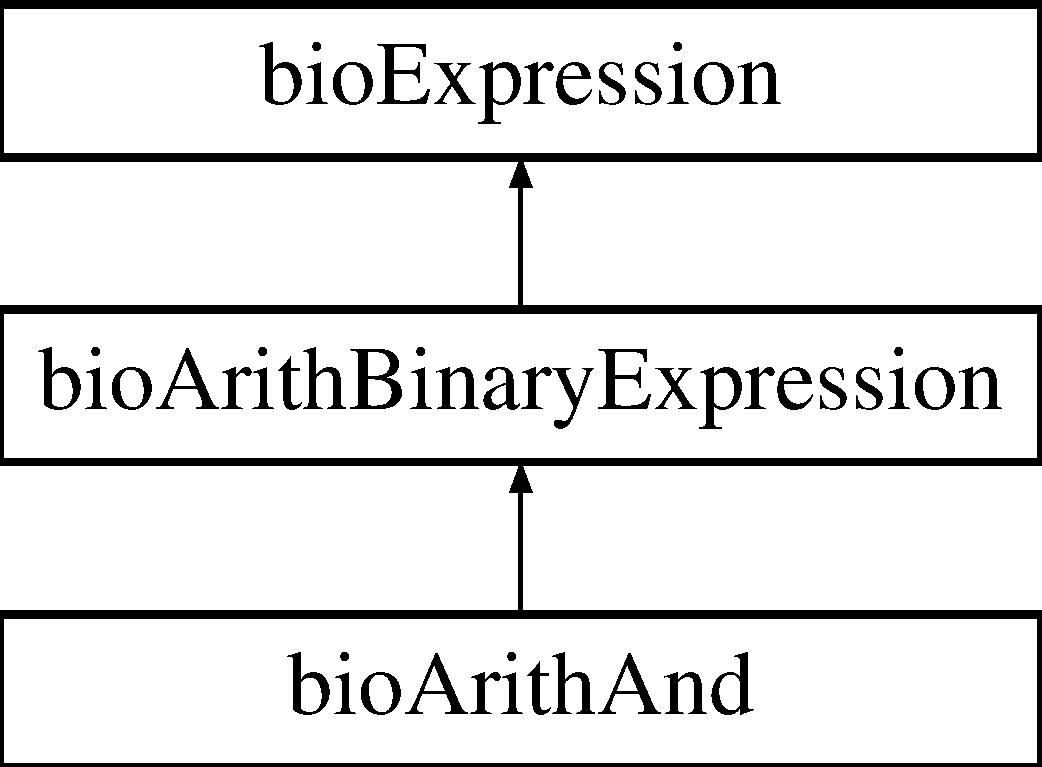
\includegraphics[height=3.000000cm]{classbio_arith_and}
\end{center}
\end{figure}
\subsection*{Public Member Functions}
\begin{DoxyCompactItemize}
\item 
\mbox{\Hypertarget{classbio_arith_and_a95f11b2bc685a1bf8d4b56217cdf2386}\label{classbio_arith_and_a95f11b2bc685a1bf8d4b56217cdf2386}} 
{\bfseries bio\+Arith\+And} (\hyperlink{classbio_expression_repository}{bio\+Expression\+Repository} $\ast$rep, pat\+U\+Long par, pat\+U\+Long left, pat\+U\+Long right, pat\+Error $\ast$\&err)
\item 
virtual pat\+String \hyperlink{classbio_arith_and_accefac4c7d08a3698bd3691e19641bfb}{get\+Operator\+Name} () const
\item 
virtual pat\+Real \hyperlink{classbio_arith_and_a3e89f3ee81dd4703fd77e5b2da1e45ad}{get\+Value} (pat\+Boolean prepare\+Gradient, pat\+U\+Long current\+Lap, pat\+Error $\ast$\&err)
\item 
virtual \hyperlink{classbio_expression}{bio\+Expression} $\ast$ \hyperlink{classbio_arith_and_a78f633a87efd5a6cbf2130032ec7100c}{get\+Derivative} (pat\+U\+Long a\+Literal\+Id, pat\+Error $\ast$\&err) const
\item 
virtual \hyperlink{classbio_arith_and}{bio\+Arith\+And} $\ast$ \hyperlink{classbio_arith_and_aa60d3a4e8d9b4684e584991a2b1effe2}{get\+Deep\+Copy} (\hyperlink{classbio_expression_repository}{bio\+Expression\+Repository} $\ast$rep, pat\+Error $\ast$\&err) const
\item 
virtual \hyperlink{classbio_arith_and}{bio\+Arith\+And} $\ast$ \hyperlink{classbio_arith_and_a3dfc8f4f9247158b3ff4c3d8e61b95ad}{get\+Shallow\+Copy} (\hyperlink{classbio_expression_repository}{bio\+Expression\+Repository} $\ast$rep, pat\+Error $\ast$\&err) const
\item 
virtual pat\+String \hyperlink{classbio_arith_and_a9b21342d9f2f1bc59bbab1596b60ed48}{get\+Expression\+String} () const
\item 
virtual \hyperlink{classbio_function_and_derivatives}{bio\+Function\+And\+Derivatives} $\ast$ \hyperlink{classbio_arith_and_af6745a5c2aca1539519d14c9e1ce5f5e}{get\+Numerical\+Function\+And\+Gradient} (vector$<$ pat\+U\+Long $>$ literal\+Ids, pat\+Boolean compute\+Hessian, pat\+Boolean debug\+Derivatives, pat\+Error $\ast$\&err)
\end{DoxyCompactItemize}
\subsection*{Additional Inherited Members}


\subsection{Detailed Description}
Class implementing a node of the tree representing a logical and operation 

\subsection{Member Function Documentation}
\mbox{\Hypertarget{classbio_arith_and_aa60d3a4e8d9b4684e584991a2b1effe2}\label{classbio_arith_and_aa60d3a4e8d9b4684e584991a2b1effe2}} 
\index{bio\+Arith\+And@{bio\+Arith\+And}!get\+Deep\+Copy@{get\+Deep\+Copy}}
\index{get\+Deep\+Copy@{get\+Deep\+Copy}!bio\+Arith\+And@{bio\+Arith\+And}}
\subsubsection{\texorpdfstring{get\+Deep\+Copy()}{getDeepCopy()}}
{\footnotesize\ttfamily \hyperlink{classbio_arith_and}{bio\+Arith\+And} $\ast$ bio\+Arith\+And\+::get\+Deep\+Copy (\begin{DoxyParamCaption}\item[{\hyperlink{classbio_expression_repository}{bio\+Expression\+Repository} $\ast$}]{rep,  }\item[{pat\+Error $\ast$\&}]{err }\end{DoxyParamCaption}) const\hspace{0.3cm}{\ttfamily [virtual]}}

Create a deep copy of the expression and returns a pointer to it. It means that new instances of the children are created. 

Reimplemented from \hyperlink{classbio_expression_a4ee1b8add634078a02eaae26cd40dcc8}{bio\+Expression}.

\mbox{\Hypertarget{classbio_arith_and_a78f633a87efd5a6cbf2130032ec7100c}\label{classbio_arith_and_a78f633a87efd5a6cbf2130032ec7100c}} 
\index{bio\+Arith\+And@{bio\+Arith\+And}!get\+Derivative@{get\+Derivative}}
\index{get\+Derivative@{get\+Derivative}!bio\+Arith\+And@{bio\+Arith\+And}}
\subsubsection{\texorpdfstring{get\+Derivative()}{getDerivative()}}
{\footnotesize\ttfamily \hyperlink{classbio_expression}{bio\+Expression} $\ast$ bio\+Arith\+And\+::get\+Derivative (\begin{DoxyParamCaption}\item[{pat\+U\+Long}]{a\+Literal\+Id,  }\item[{pat\+Error $\ast$\&}]{err }\end{DoxyParamCaption}) const\hspace{0.3cm}{\ttfamily [virtual]}}

\begin{DoxyReturn}{Returns}
value of the derivative w.\+r.\+t literal 
\end{DoxyReturn}

\begin{DoxyParams}{Parameters}
{\em index} & of the literal involved in the derivative \\
\hline
{\em err} & ref. of the pointer to the error object. \\
\hline
\end{DoxyParams}


Reimplemented from \hyperlink{classbio_expression_a5915579d1193f25f216c1e273c97f2ce}{bio\+Expression}.

\mbox{\Hypertarget{classbio_arith_and_a9b21342d9f2f1bc59bbab1596b60ed48}\label{classbio_arith_and_a9b21342d9f2f1bc59bbab1596b60ed48}} 
\index{bio\+Arith\+And@{bio\+Arith\+And}!get\+Expression\+String@{get\+Expression\+String}}
\index{get\+Expression\+String@{get\+Expression\+String}!bio\+Arith\+And@{bio\+Arith\+And}}
\subsubsection{\texorpdfstring{get\+Expression\+String()}{getExpressionString()}}
{\footnotesize\ttfamily pat\+String bio\+Arith\+And\+::get\+Expression\+String (\begin{DoxyParamCaption}{ }\end{DoxyParamCaption}) const\hspace{0.3cm}{\ttfamily [virtual]}}

Compute a string that represents the expression. It is designed to replace the expression itself when used only for comparison purposes. Code\+: +\{expr1\}\{expr2\}\+: binary plus -\/\{expr1\}\{expr2\}\+: binary minus \{expr1\}\{expr2\}\+: multiplication /\{expr1\}\{expr2\}\+: division $^\wedge$\{expr1\}\{expr2\}\+: power \&\{expr1\}\{expr2\}\+: and $\vert$\{expr1\}\{expr2\}\+: or =\{expr1\}\{expr2\}\+: equal !=\{expr1\}\{expr2\}\+: not equal $<$\{expr1\}\{expr2\}\+: lesser than $<$=\{expr1\}\{expr2\}\+: lesser or equal to $>$\{expr1\}\{expr2\}\+: greater than $>$=\{expr1\}\{expr2\}\+: greater or equal to \$A\{expr\}\+: abs \$D\mbox{[}expr\mbox{]}\mbox{[}\{expr1\}...\{exprN\}\mbox{]}\+: dictionary (\hyperlink{classbio_arith_elem}{bio\+Arith\+Elem}) \$E\{expr\}\+: exp \$L\{expr\}\+: log \$M\{expr\}\+: Unary minus \$\+Piterator\+\_\+name\{expr\}\+: prod \$Q\{string1\}\{string2\}\+: sequence \$\+Siterator\+\_\+name\{expr\}\+: sum \$\+Ziterator\+\_\+name\mbox{[}\{expr1\}...\{exprN\}\mbox{]}\+: merged sum \{expr1\}\{expr2\}...\{exprN\}//\+: list of expressions number\+: constant \#id\+: literal \&id\+: random 

Reimplemented from \hyperlink{classbio_expression_a3e4b4dca58dbbc6f0e411b30eb3f60b4}{bio\+Expression}.

\mbox{\Hypertarget{classbio_arith_and_af6745a5c2aca1539519d14c9e1ce5f5e}\label{classbio_arith_and_af6745a5c2aca1539519d14c9e1ce5f5e}} 
\index{bio\+Arith\+And@{bio\+Arith\+And}!get\+Numerical\+Function\+And\+Gradient@{get\+Numerical\+Function\+And\+Gradient}}
\index{get\+Numerical\+Function\+And\+Gradient@{get\+Numerical\+Function\+And\+Gradient}!bio\+Arith\+And@{bio\+Arith\+And}}
\subsubsection{\texorpdfstring{get\+Numerical\+Function\+And\+Gradient()}{getNumericalFunctionAndGradient()}}
{\footnotesize\ttfamily \hyperlink{classbio_function_and_derivatives}{bio\+Function\+And\+Derivatives} $\ast$ bio\+Arith\+And\+::get\+Numerical\+Function\+And\+Gradient (\begin{DoxyParamCaption}\item[{vector$<$ pat\+U\+Long $>$}]{literal\+Ids,  }\item[{pat\+Boolean}]{compute\+Hessian,  }\item[{pat\+Boolean}]{debug\+Derivatives,  }\item[{pat\+Error $\ast$\&}]{err }\end{DoxyParamCaption})\hspace{0.3cm}{\ttfamily [virtual]}}

\begin{DoxyReturn}{Returns}
value and gradient of the expression 
\end{DoxyReturn}

\begin{DoxyParams}{Parameters}
{\em err} & ref. of the pointer to the error object. \\
\hline
\end{DoxyParams}


Reimplemented from \hyperlink{classbio_expression_a91c81ce80c9e972c913b10f5f3c1ed13}{bio\+Expression}.

\mbox{\Hypertarget{classbio_arith_and_accefac4c7d08a3698bd3691e19641bfb}\label{classbio_arith_and_accefac4c7d08a3698bd3691e19641bfb}} 
\index{bio\+Arith\+And@{bio\+Arith\+And}!get\+Operator\+Name@{get\+Operator\+Name}}
\index{get\+Operator\+Name@{get\+Operator\+Name}!bio\+Arith\+And@{bio\+Arith\+And}}
\subsubsection{\texorpdfstring{get\+Operator\+Name()}{getOperatorName()}}
{\footnotesize\ttfamily pat\+String bio\+Arith\+And\+::get\+Operator\+Name (\begin{DoxyParamCaption}{ }\end{DoxyParamCaption}) const\hspace{0.3cm}{\ttfamily [virtual]}}

\begin{DoxyReturn}{Returns}
name of the operator 
\end{DoxyReturn}


Reimplemented from \hyperlink{classbio_expression_a2353a4afb3a2b0af7c63aba086a72bde}{bio\+Expression}.

\mbox{\Hypertarget{classbio_arith_and_a3dfc8f4f9247158b3ff4c3d8e61b95ad}\label{classbio_arith_and_a3dfc8f4f9247158b3ff4c3d8e61b95ad}} 
\index{bio\+Arith\+And@{bio\+Arith\+And}!get\+Shallow\+Copy@{get\+Shallow\+Copy}}
\index{get\+Shallow\+Copy@{get\+Shallow\+Copy}!bio\+Arith\+And@{bio\+Arith\+And}}
\subsubsection{\texorpdfstring{get\+Shallow\+Copy()}{getShallowCopy()}}
{\footnotesize\ttfamily \hyperlink{classbio_arith_and}{bio\+Arith\+And} $\ast$ bio\+Arith\+And\+::get\+Shallow\+Copy (\begin{DoxyParamCaption}\item[{\hyperlink{classbio_expression_repository}{bio\+Expression\+Repository} $\ast$}]{rep,  }\item[{pat\+Error $\ast$\&}]{err }\end{DoxyParamCaption}) const\hspace{0.3cm}{\ttfamily [virtual]}}

Create a shallow copy of the expression and returns a pointer to it. It means that no new instance of the children are created. It is typically called by the repository 

Reimplemented from \hyperlink{classbio_expression_a442534762693b92baaf33928979a1bf8}{bio\+Expression}.

\mbox{\Hypertarget{classbio_arith_and_a3e89f3ee81dd4703fd77e5b2da1e45ad}\label{classbio_arith_and_a3e89f3ee81dd4703fd77e5b2da1e45ad}} 
\index{bio\+Arith\+And@{bio\+Arith\+And}!get\+Value@{get\+Value}}
\index{get\+Value@{get\+Value}!bio\+Arith\+And@{bio\+Arith\+And}}
\subsubsection{\texorpdfstring{get\+Value()}{getValue()}}
{\footnotesize\ttfamily pat\+Real bio\+Arith\+And\+::get\+Value (\begin{DoxyParamCaption}\item[{pat\+Boolean}]{prepare\+Gradient,  }\item[{pat\+U\+Long}]{current\+Lap,  }\item[{pat\+Error $\ast$\&}]{err }\end{DoxyParamCaption})\hspace{0.3cm}{\ttfamily [virtual]}}

\begin{DoxyReturn}{Returns}
value of the expression 
\end{DoxyReturn}

\begin{DoxyParams}{Parameters}
{\em err} & ref. of the pointer to the error object. \\
\hline
\end{DoxyParams}


Reimplemented from \hyperlink{classbio_expression_af58662a5d4d456f15bc4f2c9bd4f8a5b}{bio\+Expression}.



The documentation for this class was generated from the following files\+:\begin{DoxyCompactItemize}
\item 
bio\+Arith\+And.\+h\item 
bio\+Arith\+And.\+cc\end{DoxyCompactItemize}

\hypertarget{classbio_arith_bayes}{}\section{bio\+Arith\+Bayes Class Reference}
\label{classbio_arith_bayes}\index{bio\+Arith\+Bayes@{bio\+Arith\+Bayes}}
Inheritance diagram for bio\+Arith\+Bayes\+:\begin{figure}[H]
\begin{center}
\leavevmode
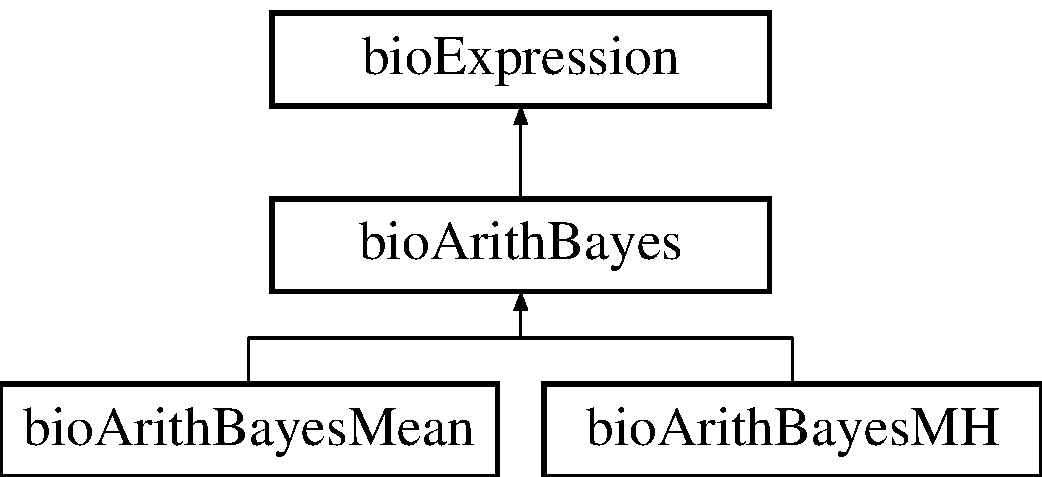
\includegraphics[height=3.000000cm]{classbio_arith_bayes}
\end{center}
\end{figure}
\subsection*{Public Member Functions}
\begin{DoxyCompactItemize}
\item 
\mbox{\Hypertarget{classbio_arith_bayes_aa832659e5def15ef3d64034ed2230421}\label{classbio_arith_bayes_aa832659e5def15ef3d64034ed2230421}} 
{\bfseries bio\+Arith\+Bayes} (\hyperlink{classbio_expression_repository}{bio\+Expression\+Repository} $\ast$rep, pat\+U\+Long par, vector$<$ pat\+U\+Long $>$ the\+Betas, pat\+Error $\ast$\&err)
\item 
\mbox{\Hypertarget{classbio_arith_bayes_a43436619a30bb17a88eeea54e34031be}\label{classbio_arith_bayes_a43436619a30bb17a88eeea54e34031be}} 
virtual \hyperlink{classbio_bayesian_results}{bio\+Bayesian\+Results} {\bfseries generate\+Draws} (pat\+Error $\ast$\&err)
\item 
virtual pat\+Real \hyperlink{classbio_arith_bayes_a7292ae29cd04168543674b1ae71f4bed}{get\+Value} (pat\+Boolean prepare\+Gradient, pat\+U\+Long current\+Lap, pat\+Error $\ast$\&err)
\item 
virtual \hyperlink{classbio_function_and_derivatives}{bio\+Function\+And\+Derivatives} $\ast$ \hyperlink{classbio_arith_bayes_a3421312ddc6b7e0b080c497cdc53d1a5}{get\+Numerical\+Function\+And\+Gradient} (vector$<$ pat\+U\+Long $>$ literal\+Ids, pat\+Boolean compute\+Hessian, pat\+Boolean debug\+Derivatives, pat\+Error $\ast$\&err)
\item 
virtual \hyperlink{classbio_expression}{bio\+Expression} $\ast$ \hyperlink{classbio_arith_bayes_a53f5d22f6a5b743fbf50bd75db697ccd}{get\+Derivative} (pat\+U\+Long a\+Literal\+Id, pat\+Error $\ast$\&err) const
\item 
\mbox{\Hypertarget{classbio_arith_bayes_a2fcca322e8e0001c5a19fbefd7b747d6}\label{classbio_arith_bayes_a2fcca322e8e0001c5a19fbefd7b747d6}} 
virtual pat\+Boolean {\bfseries is\+Bayesian} () const
\item 
\mbox{\Hypertarget{classbio_arith_bayes_a96e6336d69bd78f9251beca5a10640f4}\label{classbio_arith_bayes_a96e6336d69bd78f9251beca5a10640f4}} 
virtual void {\bfseries get\+Next\+Draw} (pat\+Error $\ast$\&err)
\end{DoxyCompactItemize}
\subsection*{Protected Attributes}
\begin{DoxyCompactItemize}
\item 
\mbox{\Hypertarget{classbio_arith_bayes_acc12626e93cfc2284925324481e4e5e3}\label{classbio_arith_bayes_acc12626e93cfc2284925324481e4e5e3}} 
vector$<$ pat\+U\+Long $>$ {\bfseries betas}
\item 
\mbox{\Hypertarget{classbio_arith_bayes_a919e7b640febedf38f99ea9e1b1bce9d}\label{classbio_arith_bayes_a919e7b640febedf38f99ea9e1b1bce9d}} 
vector$<$ vector$<$ pat\+Real $>$ $>$ {\bfseries the\+Draws}
\item 
\mbox{\Hypertarget{classbio_arith_bayes_af1a8a772dac8eac243a2813b3fbd378b}\label{classbio_arith_bayes_af1a8a772dac8eac243a2813b3fbd378b}} 
vector$<$ pat\+Real $>$ {\bfseries beta\+Values}
\item 
\mbox{\Hypertarget{classbio_arith_bayes_a967ec67d4d7ea0905b64905e8f81ea33}\label{classbio_arith_bayes_a967ec67d4d7ea0905b64905e8f81ea33}} 
vector$<$ \hyperlink{classbio_expression}{bio\+Expression} $\ast$ $>$ {\bfseries betas\+Expr}
\item 
\mbox{\Hypertarget{classbio_arith_bayes_ab549c547068e12f61da48efd39391195}\label{classbio_arith_bayes_ab549c547068e12f61da48efd39391195}} 
vector$<$ pat\+String $>$ {\bfseries beta\+Names}
\item 
\mbox{\Hypertarget{classbio_arith_bayes_ad87851021a53ac4dabe7194d1ec7370d}\label{classbio_arith_bayes_ad87851021a53ac4dabe7194d1ec7370d}} 
pat\+Normal\+Wichura $\ast$ {\bfseries the\+Normal}
\item 
\mbox{\Hypertarget{classbio_arith_bayes_a7ad02ee9a4b5d6515c4523f8cc62bd78}\label{classbio_arith_bayes_a7ad02ee9a4b5d6515c4523f8cc62bd78}} 
pat\+Uniform $\ast$ {\bfseries the\+Uniform}
\end{DoxyCompactItemize}


\subsection{Member Function Documentation}
\mbox{\Hypertarget{classbio_arith_bayes_a53f5d22f6a5b743fbf50bd75db697ccd}\label{classbio_arith_bayes_a53f5d22f6a5b743fbf50bd75db697ccd}} 
\index{bio\+Arith\+Bayes@{bio\+Arith\+Bayes}!get\+Derivative@{get\+Derivative}}
\index{get\+Derivative@{get\+Derivative}!bio\+Arith\+Bayes@{bio\+Arith\+Bayes}}
\subsubsection{\texorpdfstring{get\+Derivative()}{getDerivative()}}
{\footnotesize\ttfamily \hyperlink{classbio_expression}{bio\+Expression} $\ast$ bio\+Arith\+Bayes\+::get\+Derivative (\begin{DoxyParamCaption}\item[{pat\+U\+Long}]{a\+Literal\+Id,  }\item[{pat\+Error $\ast$\&}]{err }\end{DoxyParamCaption}) const\hspace{0.3cm}{\ttfamily [virtual]}}

\begin{DoxyReturn}{Returns}
value of the derivative w.\+r.\+t literal 
\end{DoxyReturn}

\begin{DoxyParams}{Parameters}
{\em index} & of the literal involved in the derivative \\
\hline
{\em err} & ref. of the pointer to the error object. \\
\hline
\end{DoxyParams}


Reimplemented from \hyperlink{classbio_expression_a5915579d1193f25f216c1e273c97f2ce}{bio\+Expression}.

\mbox{\Hypertarget{classbio_arith_bayes_a3421312ddc6b7e0b080c497cdc53d1a5}\label{classbio_arith_bayes_a3421312ddc6b7e0b080c497cdc53d1a5}} 
\index{bio\+Arith\+Bayes@{bio\+Arith\+Bayes}!get\+Numerical\+Function\+And\+Gradient@{get\+Numerical\+Function\+And\+Gradient}}
\index{get\+Numerical\+Function\+And\+Gradient@{get\+Numerical\+Function\+And\+Gradient}!bio\+Arith\+Bayes@{bio\+Arith\+Bayes}}
\subsubsection{\texorpdfstring{get\+Numerical\+Function\+And\+Gradient()}{getNumericalFunctionAndGradient()}}
{\footnotesize\ttfamily \hyperlink{classbio_function_and_derivatives}{bio\+Function\+And\+Derivatives} $\ast$ bio\+Arith\+Bayes\+::get\+Numerical\+Function\+And\+Gradient (\begin{DoxyParamCaption}\item[{vector$<$ pat\+U\+Long $>$}]{literal\+Ids,  }\item[{pat\+Boolean}]{compute\+Hessian,  }\item[{pat\+Boolean}]{debug\+Derivatives,  }\item[{pat\+Error $\ast$\&}]{err }\end{DoxyParamCaption})\hspace{0.3cm}{\ttfamily [virtual]}}

\begin{DoxyReturn}{Returns}
value and gradient of the expression 
\end{DoxyReturn}

\begin{DoxyParams}{Parameters}
{\em err} & ref. of the pointer to the error object. \\
\hline
\end{DoxyParams}


Reimplemented from \hyperlink{classbio_expression_a91c81ce80c9e972c913b10f5f3c1ed13}{bio\+Expression}.

\mbox{\Hypertarget{classbio_arith_bayes_a7292ae29cd04168543674b1ae71f4bed}\label{classbio_arith_bayes_a7292ae29cd04168543674b1ae71f4bed}} 
\index{bio\+Arith\+Bayes@{bio\+Arith\+Bayes}!get\+Value@{get\+Value}}
\index{get\+Value@{get\+Value}!bio\+Arith\+Bayes@{bio\+Arith\+Bayes}}
\subsubsection{\texorpdfstring{get\+Value()}{getValue()}}
{\footnotesize\ttfamily pat\+Real bio\+Arith\+Bayes\+::get\+Value (\begin{DoxyParamCaption}\item[{pat\+Boolean}]{prepare\+Gradient,  }\item[{pat\+U\+Long}]{current\+Lap,  }\item[{pat\+Error $\ast$\&}]{err }\end{DoxyParamCaption})\hspace{0.3cm}{\ttfamily [virtual]}}

\begin{DoxyReturn}{Returns}
value of the expression 
\end{DoxyReturn}

\begin{DoxyParams}{Parameters}
{\em err} & ref. of the pointer to the error object. \\
\hline
\end{DoxyParams}


Reimplemented from \hyperlink{classbio_expression_af58662a5d4d456f15bc4f2c9bd4f8a5b}{bio\+Expression}.



The documentation for this class was generated from the following files\+:\begin{DoxyCompactItemize}
\item 
bio\+Arith\+Bayes.\+h\item 
bio\+Arith\+Bayes.\+cc\end{DoxyCompactItemize}

\hypertarget{classbio_arith_bayes_mean}{}\section{bio\+Arith\+Bayes\+Mean Class Reference}
\label{classbio_arith_bayes_mean}\index{bio\+Arith\+Bayes\+Mean@{bio\+Arith\+Bayes\+Mean}}
Inheritance diagram for bio\+Arith\+Bayes\+Mean\+:\begin{figure}[H]
\begin{center}
\leavevmode
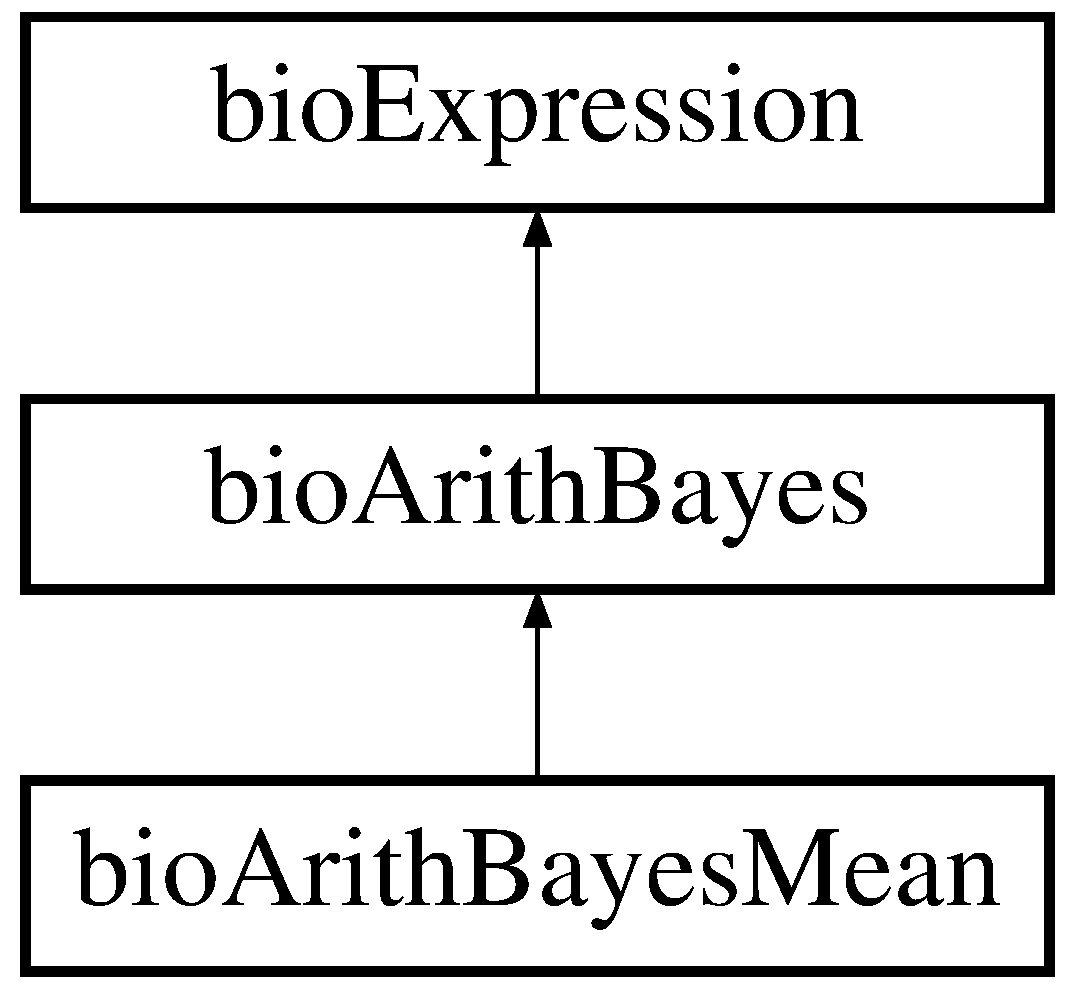
\includegraphics[height=3.000000cm]{classbio_arith_bayes_mean}
\end{center}
\end{figure}
\subsection*{Public Member Functions}
\begin{DoxyCompactItemize}
\item 
\mbox{\Hypertarget{classbio_arith_bayes_mean_a5e958254c919ea1a181540bea2c64736}\label{classbio_arith_bayes_mean_a5e958254c919ea1a181540bea2c64736}} 
{\bfseries bio\+Arith\+Bayes\+Mean} (\hyperlink{classbio_expression_repository}{bio\+Expression\+Repository} $\ast$rep, pat\+U\+Long par, vector$<$ pat\+U\+Long $>$ means, vector$<$ pat\+U\+Long $>$ realizations, vector$<$ vector$<$ pat\+U\+Long $>$ $>$ varcovar, pat\+Error $\ast$\&err)
\item 
pat\+String \hyperlink{classbio_arith_bayes_mean_a681e8636e50c05683a0d89170a264ac9}{get\+Operator\+Name} () const
\item 
pat\+String \hyperlink{classbio_arith_bayes_mean_a334b29ea459dc9f8943f888595dc4aa5}{get\+Expression} (pat\+Error $\ast$\&err) const
\item 
\hyperlink{classbio_arith_bayes_mean}{bio\+Arith\+Bayes\+Mean} $\ast$ \hyperlink{classbio_arith_bayes_mean_ac37c22c5d01ae43834f930a39bca5039}{get\+Deep\+Copy} (\hyperlink{classbio_expression_repository}{bio\+Expression\+Repository} $\ast$rep, pat\+Error $\ast$\&err) const
\item 
\hyperlink{classbio_arith_bayes_mean}{bio\+Arith\+Bayes\+Mean} $\ast$ \hyperlink{classbio_arith_bayes_mean_a1cee3c48858490ec488b2754c32c56f2}{get\+Shallow\+Copy} (\hyperlink{classbio_expression_repository}{bio\+Expression\+Repository} $\ast$rep, pat\+Error $\ast$\&err) const
\item 
\mbox{\Hypertarget{classbio_arith_bayes_mean_a7c85429c6fb48fe19b5731d200f7e748}\label{classbio_arith_bayes_mean_a7c85429c6fb48fe19b5731d200f7e748}} 
pat\+Boolean {\bfseries depends\+Of} (pat\+U\+Long a\+Literal\+Id) const
\item 
pat\+String \hyperlink{classbio_arith_bayes_mean_a240a65d98274bae45da8203db5a96754}{get\+Expression\+String} () const
\item 
\mbox{\Hypertarget{classbio_arith_bayes_mean_ad90697c64d51c7afdafb3dd30cac9980}\label{classbio_arith_bayes_mean_ad90697c64d51c7afdafb3dd30cac9980}} 
virtual pat\+U\+Long {\bfseries get\+Number\+Of\+Operations} () const
\item 
\mbox{\Hypertarget{classbio_arith_bayes_mean_a8f14b45d74d6860988db43f2393a80de}\label{classbio_arith_bayes_mean_a8f14b45d74d6860988db43f2393a80de}} 
virtual pat\+Boolean {\bfseries contains\+An\+Iterator} () const
\item 
\mbox{\Hypertarget{classbio_arith_bayes_mean_a11bcb7619df3d8203b651ecf26ff2cf9}\label{classbio_arith_bayes_mean_a11bcb7619df3d8203b651ecf26ff2cf9}} 
virtual pat\+Boolean {\bfseries contains\+An\+Iterator\+On\+Rows} () const
\item 
\mbox{\Hypertarget{classbio_arith_bayes_mean_a0d451cf413da02b78b2111157d36c6a7}\label{classbio_arith_bayes_mean_a0d451cf413da02b78b2111157d36c6a7}} 
virtual pat\+Boolean {\bfseries contains\+An\+Integral} () const
\item 
\mbox{\Hypertarget{classbio_arith_bayes_mean_ace10f529d0005ba435b6db5613cfbb77}\label{classbio_arith_bayes_mean_ace10f529d0005ba435b6db5613cfbb77}} 
virtual pat\+Boolean {\bfseries contains\+A\+Sequence} () const
\item 
\mbox{\Hypertarget{classbio_arith_bayes_mean_ad397eeeb6fb7a7b08438e08bfb71b02c}\label{classbio_arith_bayes_mean_ad397eeeb6fb7a7b08438e08bfb71b02c}} 
virtual void {\bfseries simplify\+Zeros} (pat\+Error $\ast$\&err)
\item 
\mbox{\Hypertarget{classbio_arith_bayes_mean_a557f40635e7c33c94fd335b900327cab}\label{classbio_arith_bayes_mean_a557f40635e7c33c94fd335b900327cab}} 
virtual void {\bfseries collect\+Expression\+Ids} (set$<$ pat\+U\+Long $>$ $\ast$s) const
\item 
\mbox{\Hypertarget{classbio_arith_bayes_mean_a0a7e77c8215f576b1f94610e8b9c8336}\label{classbio_arith_bayes_mean_a0a7e77c8215f576b1f94610e8b9c8336}} 
virtual pat\+String {\bfseries check} (pat\+Error $\ast$\&err) const
\item 
\mbox{\Hypertarget{classbio_arith_bayes_mean_ac7950e267386a7c0b2a44806262f5ef1}\label{classbio_arith_bayes_mean_ac7950e267386a7c0b2a44806262f5ef1}} 
void {\bfseries get\+Next\+Draw} (pat\+Error $\ast$\&err)
\end{DoxyCompactItemize}
\subsection*{Additional Inherited Members}


\subsection{Member Function Documentation}
\mbox{\Hypertarget{classbio_arith_bayes_mean_ac37c22c5d01ae43834f930a39bca5039}\label{classbio_arith_bayes_mean_ac37c22c5d01ae43834f930a39bca5039}} 
\index{bio\+Arith\+Bayes\+Mean@{bio\+Arith\+Bayes\+Mean}!get\+Deep\+Copy@{get\+Deep\+Copy}}
\index{get\+Deep\+Copy@{get\+Deep\+Copy}!bio\+Arith\+Bayes\+Mean@{bio\+Arith\+Bayes\+Mean}}
\subsubsection{\texorpdfstring{get\+Deep\+Copy()}{getDeepCopy()}}
{\footnotesize\ttfamily \hyperlink{classbio_arith_bayes_mean}{bio\+Arith\+Bayes\+Mean} $\ast$ bio\+Arith\+Bayes\+Mean\+::get\+Deep\+Copy (\begin{DoxyParamCaption}\item[{\hyperlink{classbio_expression_repository}{bio\+Expression\+Repository} $\ast$}]{rep,  }\item[{pat\+Error $\ast$\&}]{err }\end{DoxyParamCaption}) const\hspace{0.3cm}{\ttfamily [virtual]}}

Create a deep copy of the expression and returns a pointer to it. It means that new instances of the children are created. 

Reimplemented from \hyperlink{classbio_expression_a4ee1b8add634078a02eaae26cd40dcc8}{bio\+Expression}.

\mbox{\Hypertarget{classbio_arith_bayes_mean_a334b29ea459dc9f8943f888595dc4aa5}\label{classbio_arith_bayes_mean_a334b29ea459dc9f8943f888595dc4aa5}} 
\index{bio\+Arith\+Bayes\+Mean@{bio\+Arith\+Bayes\+Mean}!get\+Expression@{get\+Expression}}
\index{get\+Expression@{get\+Expression}!bio\+Arith\+Bayes\+Mean@{bio\+Arith\+Bayes\+Mean}}
\subsubsection{\texorpdfstring{get\+Expression()}{getExpression()}}
{\footnotesize\ttfamily pat\+String bio\+Arith\+Bayes\+Mean\+::get\+Expression (\begin{DoxyParamCaption}\item[{pat\+Error $\ast$\&}]{err }\end{DoxyParamCaption}) const\hspace{0.3cm}{\ttfamily [virtual]}}

\begin{DoxyReturn}{Returns}
printed expression 
\end{DoxyReturn}


Reimplemented from \hyperlink{classbio_expression_a66a83eb0caac18dd5e568ffde5a8b5d4}{bio\+Expression}.

\mbox{\Hypertarget{classbio_arith_bayes_mean_a240a65d98274bae45da8203db5a96754}\label{classbio_arith_bayes_mean_a240a65d98274bae45da8203db5a96754}} 
\index{bio\+Arith\+Bayes\+Mean@{bio\+Arith\+Bayes\+Mean}!get\+Expression\+String@{get\+Expression\+String}}
\index{get\+Expression\+String@{get\+Expression\+String}!bio\+Arith\+Bayes\+Mean@{bio\+Arith\+Bayes\+Mean}}
\subsubsection{\texorpdfstring{get\+Expression\+String()}{getExpressionString()}}
{\footnotesize\ttfamily pat\+String bio\+Arith\+Bayes\+Mean\+::get\+Expression\+String (\begin{DoxyParamCaption}{ }\end{DoxyParamCaption}) const\hspace{0.3cm}{\ttfamily [virtual]}}

Compute a string that represents the expression. It is designed to replace the expression itself when used only for comparison purposes. Code\+: +\{expr1\}\{expr2\}\+: binary plus -\/\{expr1\}\{expr2\}\+: binary minus \{expr1\}\{expr2\}\+: multiplication /\{expr1\}\{expr2\}\+: division $^\wedge$\{expr1\}\{expr2\}\+: power \&\{expr1\}\{expr2\}\+: and $\vert$\{expr1\}\{expr2\}\+: or =\{expr1\}\{expr2\}\+: equal !=\{expr1\}\{expr2\}\+: not equal $<$\{expr1\}\{expr2\}\+: lesser than $<$=\{expr1\}\{expr2\}\+: lesser or equal to $>$\{expr1\}\{expr2\}\+: greater than $>$=\{expr1\}\{expr2\}\+: greater or equal to \$A\{expr\}\+: abs \$D\mbox{[}expr\mbox{]}\mbox{[}\{expr1\}...\{exprN\}\mbox{]}\+: dictionary (\hyperlink{classbio_arith_elem}{bio\+Arith\+Elem}) \$E\{expr\}\+: exp \$L\{expr\}\+: log \$M\{expr\}\+: Unary minus \$\+Piterator\+\_\+name\{expr\}\+: prod \$Q\{string1\}\{string2\}\+: sequence \$\+Siterator\+\_\+name\{expr\}\+: sum \$\+Ziterator\+\_\+name\mbox{[}\{expr1\}...\{exprN\}\mbox{]}\+: merged sum \{expr1\}\{expr2\}...\{exprN\}//\+: list of expressions number\+: constant \#id\+: literal \&id\+: random 

Reimplemented from \hyperlink{classbio_expression_a3e4b4dca58dbbc6f0e411b30eb3f60b4}{bio\+Expression}.

\mbox{\Hypertarget{classbio_arith_bayes_mean_a681e8636e50c05683a0d89170a264ac9}\label{classbio_arith_bayes_mean_a681e8636e50c05683a0d89170a264ac9}} 
\index{bio\+Arith\+Bayes\+Mean@{bio\+Arith\+Bayes\+Mean}!get\+Operator\+Name@{get\+Operator\+Name}}
\index{get\+Operator\+Name@{get\+Operator\+Name}!bio\+Arith\+Bayes\+Mean@{bio\+Arith\+Bayes\+Mean}}
\subsubsection{\texorpdfstring{get\+Operator\+Name()}{getOperatorName()}}
{\footnotesize\ttfamily pat\+String bio\+Arith\+Bayes\+Mean\+::get\+Operator\+Name (\begin{DoxyParamCaption}{ }\end{DoxyParamCaption}) const\hspace{0.3cm}{\ttfamily [virtual]}}

\begin{DoxyReturn}{Returns}
name of the operator 
\end{DoxyReturn}


Reimplemented from \hyperlink{classbio_expression_a2353a4afb3a2b0af7c63aba086a72bde}{bio\+Expression}.

\mbox{\Hypertarget{classbio_arith_bayes_mean_a1cee3c48858490ec488b2754c32c56f2}\label{classbio_arith_bayes_mean_a1cee3c48858490ec488b2754c32c56f2}} 
\index{bio\+Arith\+Bayes\+Mean@{bio\+Arith\+Bayes\+Mean}!get\+Shallow\+Copy@{get\+Shallow\+Copy}}
\index{get\+Shallow\+Copy@{get\+Shallow\+Copy}!bio\+Arith\+Bayes\+Mean@{bio\+Arith\+Bayes\+Mean}}
\subsubsection{\texorpdfstring{get\+Shallow\+Copy()}{getShallowCopy()}}
{\footnotesize\ttfamily \hyperlink{classbio_arith_bayes_mean}{bio\+Arith\+Bayes\+Mean} $\ast$ bio\+Arith\+Bayes\+Mean\+::get\+Shallow\+Copy (\begin{DoxyParamCaption}\item[{\hyperlink{classbio_expression_repository}{bio\+Expression\+Repository} $\ast$}]{rep,  }\item[{pat\+Error $\ast$\&}]{err }\end{DoxyParamCaption}) const\hspace{0.3cm}{\ttfamily [virtual]}}

Create a shallow copy of the expression and returns a pointer to it. It means that no new instance of the children are created. It is typically called by the repository 

Reimplemented from \hyperlink{classbio_expression_a442534762693b92baaf33928979a1bf8}{bio\+Expression}.



The documentation for this class was generated from the following files\+:\begin{DoxyCompactItemize}
\item 
bio\+Arith\+Bayes\+Mean.\+h\item 
bio\+Arith\+Bayes\+Mean.\+cc\end{DoxyCompactItemize}

\hypertarget{classbio_arith_bayes_m_h}{}\section{bio\+Arith\+Bayes\+MH Class Reference}
\label{classbio_arith_bayes_m_h}\index{bio\+Arith\+Bayes\+MH@{bio\+Arith\+Bayes\+MH}}


{\ttfamily \#include $<$bio\+Arith\+Bayes\+M\+H.\+h$>$}

Inheritance diagram for bio\+Arith\+Bayes\+MH\+:\begin{figure}[H]
\begin{center}
\leavevmode
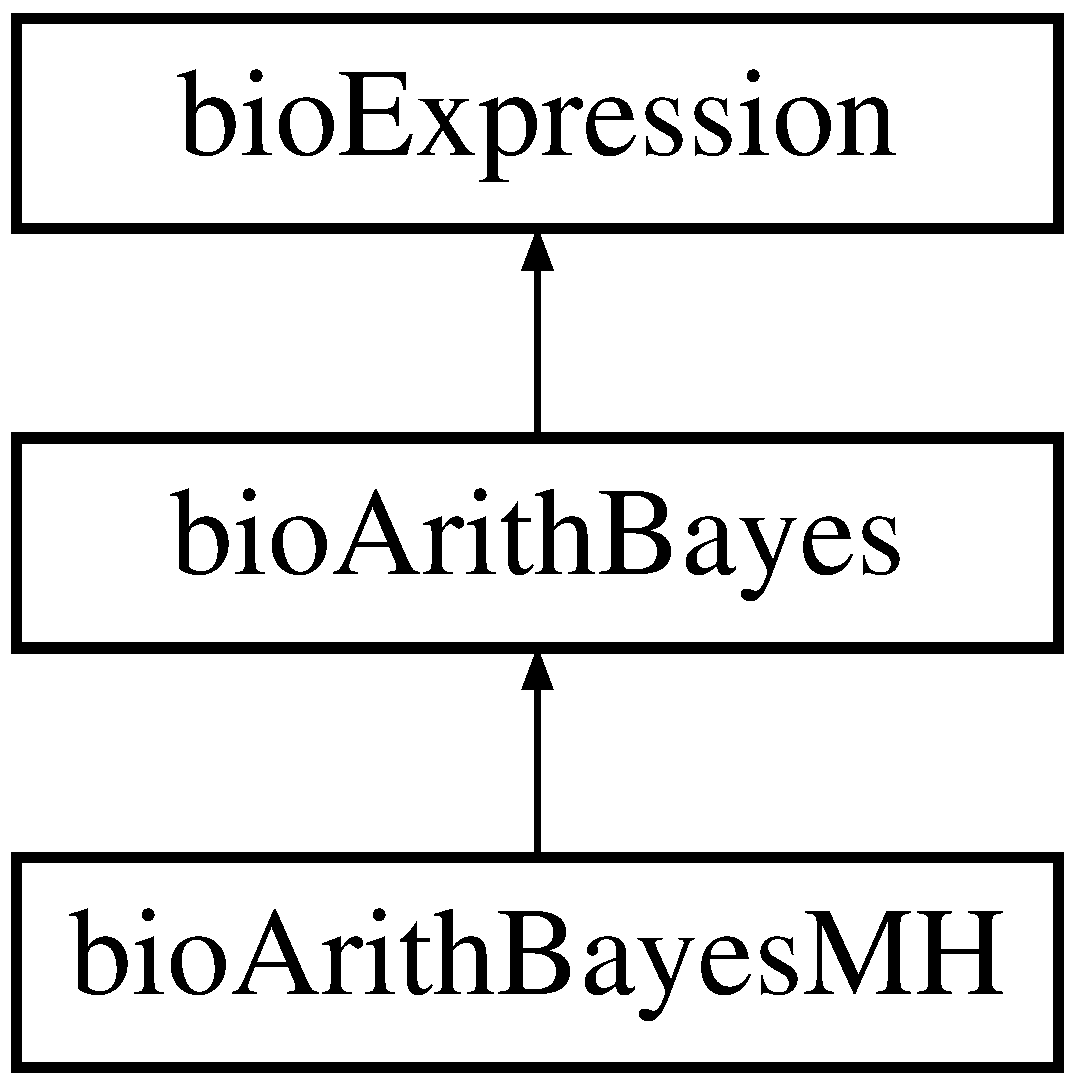
\includegraphics[height=3.000000cm]{classbio_arith_bayes_m_h}
\end{center}
\end{figure}
\subsection*{Public Member Functions}
\begin{DoxyCompactItemize}
\item 
\mbox{\Hypertarget{classbio_arith_bayes_m_h_a2fb0d44775923779ed7ba9f4274537e2}\label{classbio_arith_bayes_m_h_a2fb0d44775923779ed7ba9f4274537e2}} 
{\bfseries bio\+Arith\+Bayes\+MH} (\hyperlink{classbio_expression_repository}{bio\+Expression\+Repository} $\ast$rep, pat\+U\+Long par, vector$<$ pat\+U\+Long $>$ the\+Betas, pat\+U\+Long the\+Density, pat\+U\+Long the\+Warmup, pat\+U\+Long the\+Steps, pat\+Error $\ast$\&err)
\item 
virtual pat\+String \hyperlink{classbio_arith_bayes_m_h_a9bf7951a901c6243af0ffc89bc5b6018}{get\+Operator\+Name} () const
\item 
virtual pat\+String \hyperlink{classbio_arith_bayes_m_h_a7579a02175af9bde0e35c0548a6740bd}{get\+Expression} (pat\+Error $\ast$\&err) const
\item 
virtual \hyperlink{classbio_arith_bayes_m_h}{bio\+Arith\+Bayes\+MH} $\ast$ \hyperlink{classbio_arith_bayes_m_h_a4477bd620cc50e05a248df51e8c74ad6}{get\+Deep\+Copy} (\hyperlink{classbio_expression_repository}{bio\+Expression\+Repository} $\ast$rep, pat\+Error $\ast$\&err) const
\item 
virtual \hyperlink{classbio_arith_bayes_m_h}{bio\+Arith\+Bayes\+MH} $\ast$ \hyperlink{classbio_arith_bayes_m_h_ab173e10b34d0eab2599ba4854f928b8f}{get\+Shallow\+Copy} (\hyperlink{classbio_expression_repository}{bio\+Expression\+Repository} $\ast$rep, pat\+Error $\ast$\&err) const
\item 
\mbox{\Hypertarget{classbio_arith_bayes_m_h_a1cfbf01cc05e45338a692510347b636c}\label{classbio_arith_bayes_m_h_a1cfbf01cc05e45338a692510347b636c}} 
virtual pat\+Boolean {\bfseries depends\+Of} (pat\+U\+Long a\+Literal\+Id) const
\item 
virtual pat\+String \hyperlink{classbio_arith_bayes_m_h_a0211e07769cd7b73f6dc344884656199}{get\+Expression\+String} () const
\item 
\mbox{\Hypertarget{classbio_arith_bayes_m_h_a80b66eeffb3aa3d2198549d3f811d047}\label{classbio_arith_bayes_m_h_a80b66eeffb3aa3d2198549d3f811d047}} 
virtual pat\+U\+Long {\bfseries get\+Number\+Of\+Operations} () const
\item 
\mbox{\Hypertarget{classbio_arith_bayes_m_h_a2db66f75cb9fe1d5fb005a53bd8e3f19}\label{classbio_arith_bayes_m_h_a2db66f75cb9fe1d5fb005a53bd8e3f19}} 
virtual pat\+Boolean {\bfseries contains\+An\+Iterator} () const
\item 
\mbox{\Hypertarget{classbio_arith_bayes_m_h_aa650cb3d15ba6689d122f54658a53911}\label{classbio_arith_bayes_m_h_aa650cb3d15ba6689d122f54658a53911}} 
virtual pat\+Boolean {\bfseries contains\+An\+Iterator\+On\+Rows} () const
\item 
\mbox{\Hypertarget{classbio_arith_bayes_m_h_a3834d4837029d2b66c4aa74848e53890}\label{classbio_arith_bayes_m_h_a3834d4837029d2b66c4aa74848e53890}} 
virtual pat\+Boolean {\bfseries contains\+An\+Integral} () const
\item 
\mbox{\Hypertarget{classbio_arith_bayes_m_h_a9d31f2a947d430b9903bcd0ce4943417}\label{classbio_arith_bayes_m_h_a9d31f2a947d430b9903bcd0ce4943417}} 
virtual pat\+Boolean {\bfseries contains\+A\+Sequence} () const
\item 
\mbox{\Hypertarget{classbio_arith_bayes_m_h_a1948c116d57eecf5508a9d17c670987d}\label{classbio_arith_bayes_m_h_a1948c116d57eecf5508a9d17c670987d}} 
virtual void {\bfseries simplify\+Zeros} (pat\+Error $\ast$\&err)
\item 
\mbox{\Hypertarget{classbio_arith_bayes_m_h_adada57d93c6a215b52b504f621556d3e}\label{classbio_arith_bayes_m_h_adada57d93c6a215b52b504f621556d3e}} 
virtual void {\bfseries collect\+Expression\+Ids} (set$<$ pat\+U\+Long $>$ $\ast$s) const
\item 
\mbox{\Hypertarget{classbio_arith_bayes_m_h_a0fcc9286993eab61ac751f41dc518efb}\label{classbio_arith_bayes_m_h_a0fcc9286993eab61ac751f41dc518efb}} 
virtual pat\+String {\bfseries check} (pat\+Error $\ast$\&err) const
\item 
\mbox{\Hypertarget{classbio_arith_bayes_m_h_a7fab1f00661fb7bacf0e618a1dc36984}\label{classbio_arith_bayes_m_h_a7fab1f00661fb7bacf0e618a1dc36984}} 
void {\bfseries initialize\+Markov\+Process} (pat\+Error $\ast$\&err)
\item 
\mbox{\Hypertarget{classbio_arith_bayes_m_h_a84261bf632f0fa9505d25bf877b62199}\label{classbio_arith_bayes_m_h_a84261bf632f0fa9505d25bf877b62199}} 
pat\+Boolean {\bfseries update\+Betas} (pat\+Error $\ast$\&err)
\item 
\mbox{\Hypertarget{classbio_arith_bayes_m_h_a7e9507046b42b230eab714f4003461f0}\label{classbio_arith_bayes_m_h_a7e9507046b42b230eab714f4003461f0}} 
virtual void {\bfseries get\+Next\+Draw} (pat\+Error $\ast$\&err)
\end{DoxyCompactItemize}
\subsection*{Additional Inherited Members}


\subsection{Detailed Description}
Class implementing a node of the tree designed for the Metropolis Hastings algorithm, to draw from a complex density 

\subsection{Member Function Documentation}
\mbox{\Hypertarget{classbio_arith_bayes_m_h_a4477bd620cc50e05a248df51e8c74ad6}\label{classbio_arith_bayes_m_h_a4477bd620cc50e05a248df51e8c74ad6}} 
\index{bio\+Arith\+Bayes\+MH@{bio\+Arith\+Bayes\+MH}!get\+Deep\+Copy@{get\+Deep\+Copy}}
\index{get\+Deep\+Copy@{get\+Deep\+Copy}!bio\+Arith\+Bayes\+MH@{bio\+Arith\+Bayes\+MH}}
\subsubsection{\texorpdfstring{get\+Deep\+Copy()}{getDeepCopy()}}
{\footnotesize\ttfamily \hyperlink{classbio_arith_bayes_m_h}{bio\+Arith\+Bayes\+MH} $\ast$ bio\+Arith\+Bayes\+M\+H\+::get\+Deep\+Copy (\begin{DoxyParamCaption}\item[{\hyperlink{classbio_expression_repository}{bio\+Expression\+Repository} $\ast$}]{rep,  }\item[{pat\+Error $\ast$\&}]{err }\end{DoxyParamCaption}) const\hspace{0.3cm}{\ttfamily [virtual]}}

Create a deep copy of the expression and returns a pointer to it. It means that new instances of the children are created. 

Reimplemented from \hyperlink{classbio_expression_a4ee1b8add634078a02eaae26cd40dcc8}{bio\+Expression}.

\mbox{\Hypertarget{classbio_arith_bayes_m_h_a7579a02175af9bde0e35c0548a6740bd}\label{classbio_arith_bayes_m_h_a7579a02175af9bde0e35c0548a6740bd}} 
\index{bio\+Arith\+Bayes\+MH@{bio\+Arith\+Bayes\+MH}!get\+Expression@{get\+Expression}}
\index{get\+Expression@{get\+Expression}!bio\+Arith\+Bayes\+MH@{bio\+Arith\+Bayes\+MH}}
\subsubsection{\texorpdfstring{get\+Expression()}{getExpression()}}
{\footnotesize\ttfamily pat\+String bio\+Arith\+Bayes\+M\+H\+::get\+Expression (\begin{DoxyParamCaption}\item[{pat\+Error $\ast$\&}]{err }\end{DoxyParamCaption}) const\hspace{0.3cm}{\ttfamily [virtual]}}

\begin{DoxyReturn}{Returns}
printed expression 
\end{DoxyReturn}


Reimplemented from \hyperlink{classbio_expression_a66a83eb0caac18dd5e568ffde5a8b5d4}{bio\+Expression}.

\mbox{\Hypertarget{classbio_arith_bayes_m_h_a0211e07769cd7b73f6dc344884656199}\label{classbio_arith_bayes_m_h_a0211e07769cd7b73f6dc344884656199}} 
\index{bio\+Arith\+Bayes\+MH@{bio\+Arith\+Bayes\+MH}!get\+Expression\+String@{get\+Expression\+String}}
\index{get\+Expression\+String@{get\+Expression\+String}!bio\+Arith\+Bayes\+MH@{bio\+Arith\+Bayes\+MH}}
\subsubsection{\texorpdfstring{get\+Expression\+String()}{getExpressionString()}}
{\footnotesize\ttfamily pat\+String bio\+Arith\+Bayes\+M\+H\+::get\+Expression\+String (\begin{DoxyParamCaption}{ }\end{DoxyParamCaption}) const\hspace{0.3cm}{\ttfamily [virtual]}}

Compute a string that represents the expression. It is designed to replace the expression itself when used only for comparison purposes. Code\+: +\{expr1\}\{expr2\}\+: binary plus -\/\{expr1\}\{expr2\}\+: binary minus \{expr1\}\{expr2\}\+: multiplication /\{expr1\}\{expr2\}\+: division $^\wedge$\{expr1\}\{expr2\}\+: power \&\{expr1\}\{expr2\}\+: and $\vert$\{expr1\}\{expr2\}\+: or =\{expr1\}\{expr2\}\+: equal !=\{expr1\}\{expr2\}\+: not equal $<$\{expr1\}\{expr2\}\+: lesser than $<$=\{expr1\}\{expr2\}\+: lesser or equal to $>$\{expr1\}\{expr2\}\+: greater than $>$=\{expr1\}\{expr2\}\+: greater or equal to \$A\{expr\}\+: abs \$D\mbox{[}expr\mbox{]}\mbox{[}\{expr1\}...\{exprN\}\mbox{]}\+: dictionary (\hyperlink{classbio_arith_elem}{bio\+Arith\+Elem}) \$E\{expr\}\+: exp \$L\{expr\}\+: log \$M\{expr\}\+: Unary minus \$\+Piterator\+\_\+name\{expr\}\+: prod \$Q\{string1\}\{string2\}\+: sequence \$\+Siterator\+\_\+name\{expr\}\+: sum \$\+Ziterator\+\_\+name\mbox{[}\{expr1\}...\{exprN\}\mbox{]}\+: merged sum \{expr1\}\{expr2\}...\{exprN\}//\+: list of expressions number\+: constant \#id\+: literal \&id\+: random 

Reimplemented from \hyperlink{classbio_expression_a3e4b4dca58dbbc6f0e411b30eb3f60b4}{bio\+Expression}.

\mbox{\Hypertarget{classbio_arith_bayes_m_h_a9bf7951a901c6243af0ffc89bc5b6018}\label{classbio_arith_bayes_m_h_a9bf7951a901c6243af0ffc89bc5b6018}} 
\index{bio\+Arith\+Bayes\+MH@{bio\+Arith\+Bayes\+MH}!get\+Operator\+Name@{get\+Operator\+Name}}
\index{get\+Operator\+Name@{get\+Operator\+Name}!bio\+Arith\+Bayes\+MH@{bio\+Arith\+Bayes\+MH}}
\subsubsection{\texorpdfstring{get\+Operator\+Name()}{getOperatorName()}}
{\footnotesize\ttfamily pat\+String bio\+Arith\+Bayes\+M\+H\+::get\+Operator\+Name (\begin{DoxyParamCaption}{ }\end{DoxyParamCaption}) const\hspace{0.3cm}{\ttfamily [virtual]}}

\begin{DoxyReturn}{Returns}
name of the operator 
\end{DoxyReturn}


Reimplemented from \hyperlink{classbio_expression_a2353a4afb3a2b0af7c63aba086a72bde}{bio\+Expression}.

\mbox{\Hypertarget{classbio_arith_bayes_m_h_ab173e10b34d0eab2599ba4854f928b8f}\label{classbio_arith_bayes_m_h_ab173e10b34d0eab2599ba4854f928b8f}} 
\index{bio\+Arith\+Bayes\+MH@{bio\+Arith\+Bayes\+MH}!get\+Shallow\+Copy@{get\+Shallow\+Copy}}
\index{get\+Shallow\+Copy@{get\+Shallow\+Copy}!bio\+Arith\+Bayes\+MH@{bio\+Arith\+Bayes\+MH}}
\subsubsection{\texorpdfstring{get\+Shallow\+Copy()}{getShallowCopy()}}
{\footnotesize\ttfamily \hyperlink{classbio_arith_bayes_m_h}{bio\+Arith\+Bayes\+MH} $\ast$ bio\+Arith\+Bayes\+M\+H\+::get\+Shallow\+Copy (\begin{DoxyParamCaption}\item[{\hyperlink{classbio_expression_repository}{bio\+Expression\+Repository} $\ast$}]{rep,  }\item[{pat\+Error $\ast$\&}]{err }\end{DoxyParamCaption}) const\hspace{0.3cm}{\ttfamily [virtual]}}

Create a shallow copy of the expression and returns a pointer to it. It means that no new instance of the children are created. It is typically called by the repository 

Reimplemented from \hyperlink{classbio_expression_a442534762693b92baaf33928979a1bf8}{bio\+Expression}.



The documentation for this class was generated from the following files\+:\begin{DoxyCompactItemize}
\item 
bio\+Arith\+Bayes\+M\+H.\+h\item 
bio\+Arith\+Bayes\+M\+H.\+cc\end{DoxyCompactItemize}

\hypertarget{classbio_arith_binary_expression}{}\section{bio\+Arith\+Binary\+Expression Class Reference}
\label{classbio_arith_binary_expression}\index{bio\+Arith\+Binary\+Expression@{bio\+Arith\+Binary\+Expression}}


{\ttfamily \#include $<$bio\+Arith\+Binary\+Expression.\+h$>$}

Inheritance diagram for bio\+Arith\+Binary\+Expression\+:\begin{figure}[H]
\begin{center}
\leavevmode
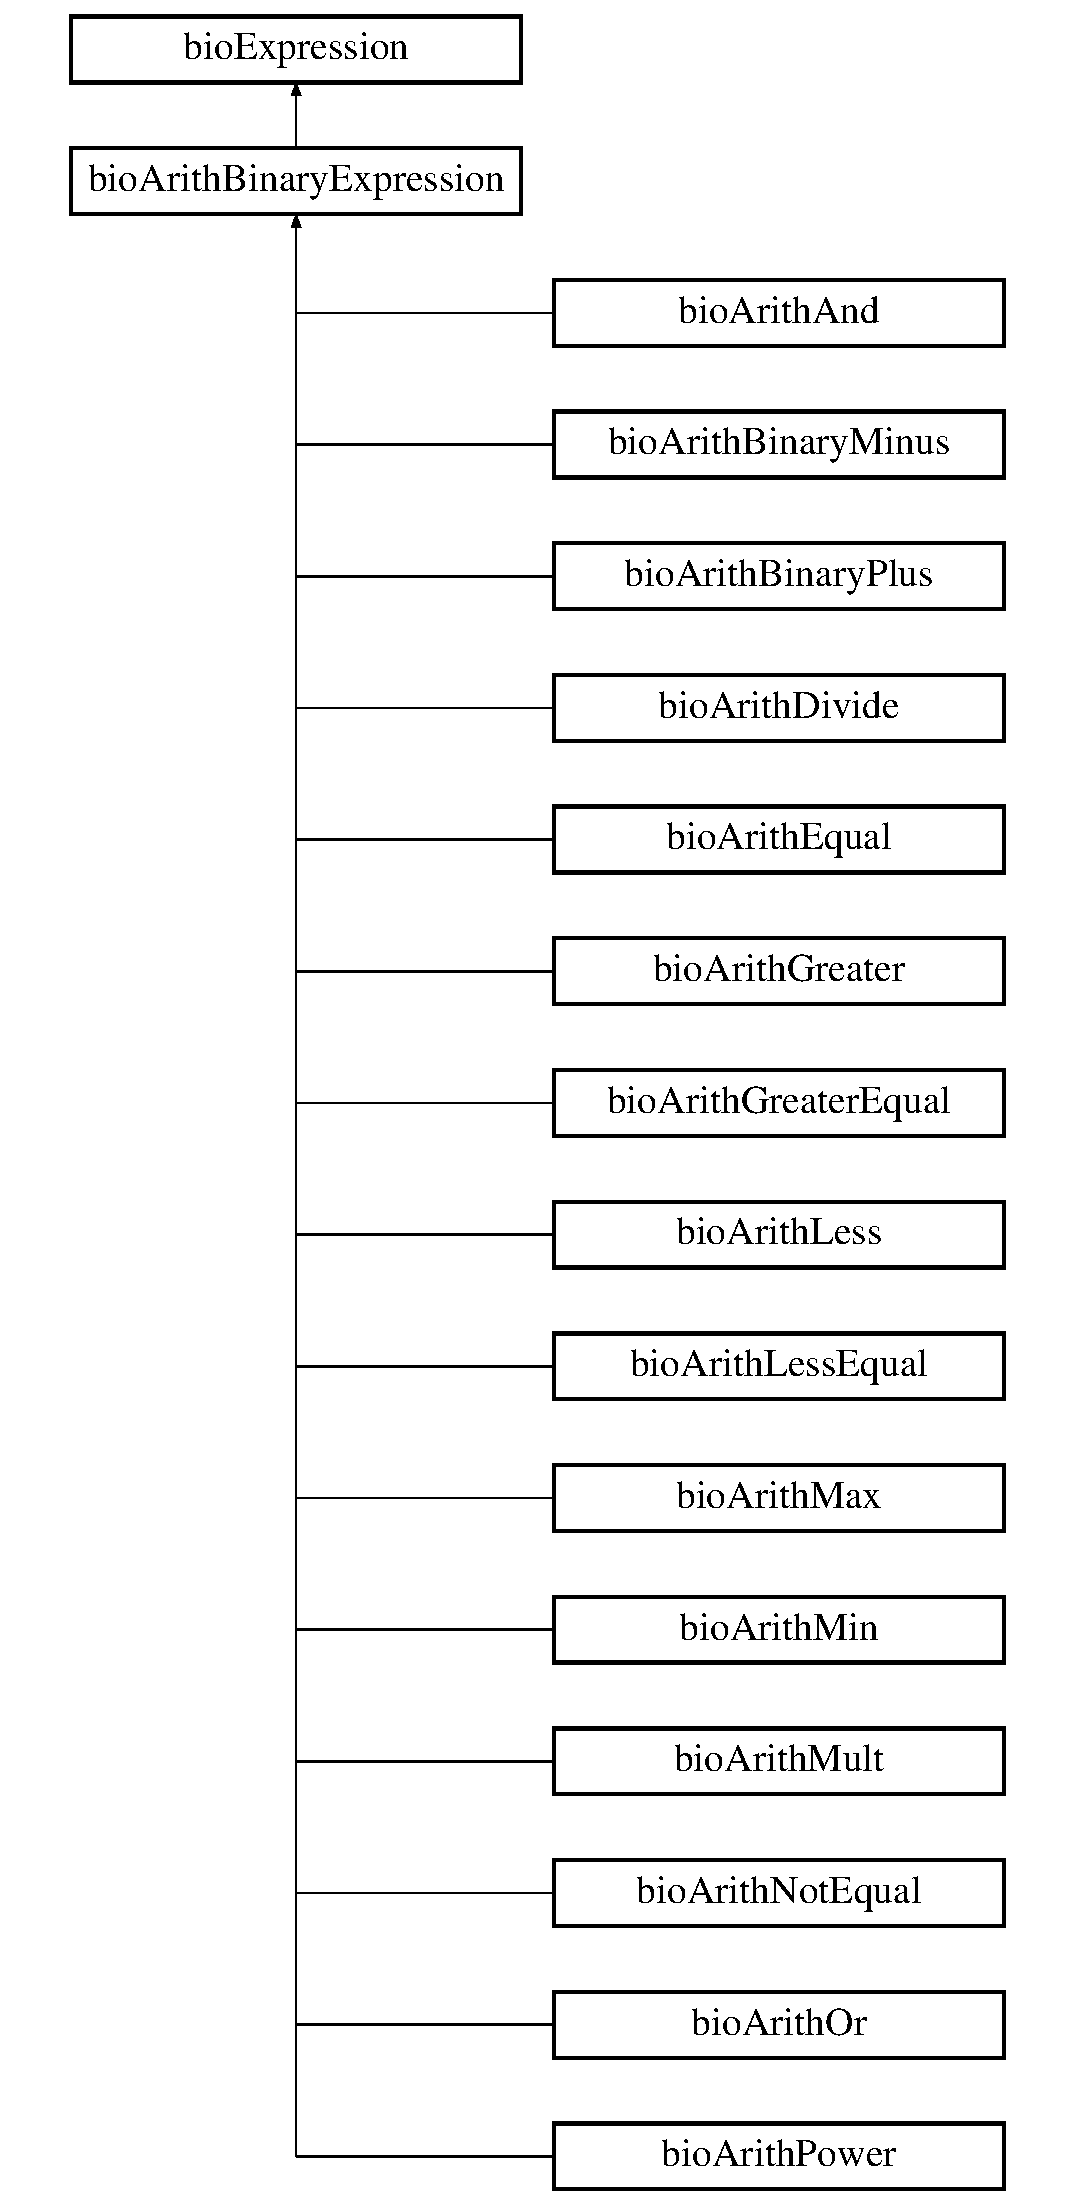
\includegraphics[height=12.000000cm]{classbio_arith_binary_expression}
\end{center}
\end{figure}
\subsection*{Public Member Functions}
\begin{DoxyCompactItemize}
\item 
\mbox{\Hypertarget{classbio_arith_binary_expression_a340b61c142b77764797950369eac7e28}\label{classbio_arith_binary_expression_a340b61c142b77764797950369eac7e28}} 
{\bfseries bio\+Arith\+Binary\+Expression} (\hyperlink{classbio_expression_repository}{bio\+Expression\+Repository} $\ast$rep, pat\+U\+Long par, pat\+U\+Long lc, pat\+U\+Long rc, pat\+Error $\ast$\&err)
\item 
\mbox{\Hypertarget{classbio_arith_binary_expression_abf82c079c5929413a6f7d412fb81ba19}\label{classbio_arith_binary_expression_abf82c079c5929413a6f7d412fb81ba19}} 
virtual \hyperlink{classbio_expression}{bio\+Expression} $\ast$ {\bfseries get\+Left\+Child} () const
\item 
\mbox{\Hypertarget{classbio_arith_binary_expression_ab1cfb7635447dd42e8b8e973c8eedc24}\label{classbio_arith_binary_expression_ab1cfb7635447dd42e8b8e973c8eedc24}} 
virtual \hyperlink{classbio_expression}{bio\+Expression} $\ast$ {\bfseries get\+Right\+Child} () const
\item 
virtual pat\+String \hyperlink{classbio_arith_binary_expression_a6c48d0f1c7b6ba1b8cf3910b9ad04f93}{get\+Expression} (pat\+Error $\ast$\&err) const
\item 
\mbox{\Hypertarget{classbio_arith_binary_expression_aab5f6ca86bb59b081d3d915bf58b83af}\label{classbio_arith_binary_expression_aab5f6ca86bb59b081d3d915bf58b83af}} 
virtual pat\+U\+Long {\bfseries get\+Number\+Of\+Operations} () const
\item 
\mbox{\Hypertarget{classbio_arith_binary_expression_af7ad9c883086f5058e1f93d9ebcf1800}\label{classbio_arith_binary_expression_af7ad9c883086f5058e1f93d9ebcf1800}} 
virtual pat\+Boolean {\bfseries depends\+Of} (pat\+U\+Long a\+Literal\+Id) const
\item 
\mbox{\Hypertarget{classbio_arith_binary_expression_add7bb73a87505b41be97b7b747e24229}\label{classbio_arith_binary_expression_add7bb73a87505b41be97b7b747e24229}} 
virtual pat\+Boolean {\bfseries contains\+An\+Iterator} () const
\item 
\mbox{\Hypertarget{classbio_arith_binary_expression_a4a91bcd3d7bb68418a0e35b33d749422}\label{classbio_arith_binary_expression_a4a91bcd3d7bb68418a0e35b33d749422}} 
virtual pat\+Boolean {\bfseries contains\+An\+Iterator\+On\+Rows} () const
\item 
\mbox{\Hypertarget{classbio_arith_binary_expression_a60b22bf5aaf9e40bafe5fb3620006d4b}\label{classbio_arith_binary_expression_a60b22bf5aaf9e40bafe5fb3620006d4b}} 
virtual pat\+Boolean {\bfseries contains\+An\+Integral} () const
\item 
\mbox{\Hypertarget{classbio_arith_binary_expression_af594a2a8aafaf291a615031972a9062c}\label{classbio_arith_binary_expression_af594a2a8aafaf291a615031972a9062c}} 
virtual pat\+Boolean {\bfseries contains\+A\+Sequence} () const
\item 
\mbox{\Hypertarget{classbio_arith_binary_expression_a1e1560a60cb3ac6a94ae9e5fcbd3307b}\label{classbio_arith_binary_expression_a1e1560a60cb3ac6a94ae9e5fcbd3307b}} 
virtual void {\bfseries simplify\+Zeros} (pat\+Error $\ast$\&err)
\item 
\mbox{\Hypertarget{classbio_arith_binary_expression_a8515e95f3de497ca7522ade60d24e308}\label{classbio_arith_binary_expression_a8515e95f3de497ca7522ade60d24e308}} 
virtual void {\bfseries collect\+Expression\+Ids} (set$<$ pat\+U\+Long $>$ $\ast$s) const
\item 
\mbox{\Hypertarget{classbio_arith_binary_expression_ad9179f665fac918f733a6d2181a7298d}\label{classbio_arith_binary_expression_ad9179f665fac918f733a6d2181a7298d}} 
virtual pat\+String {\bfseries check} (pat\+Error $\ast$\&err) const
\end{DoxyCompactItemize}
\subsection*{Protected Attributes}
\begin{DoxyCompactItemize}
\item 
\mbox{\Hypertarget{classbio_arith_binary_expression_a6fb23227582cda20c43541ce35767e2d}\label{classbio_arith_binary_expression_a6fb23227582cda20c43541ce35767e2d}} 
pat\+U\+Long {\bfseries left\+Child\+Id}
\item 
\mbox{\Hypertarget{classbio_arith_binary_expression_a62727cdbc8f6518c14e08eafc9965cab}\label{classbio_arith_binary_expression_a62727cdbc8f6518c14e08eafc9965cab}} 
pat\+U\+Long {\bfseries right\+Child\+Id}
\item 
\mbox{\Hypertarget{classbio_arith_binary_expression_a99815db34d52903224e468ef574e5869}\label{classbio_arith_binary_expression_a99815db34d52903224e468ef574e5869}} 
\hyperlink{classbio_expression}{bio\+Expression} $\ast$ {\bfseries left\+Child}
\item 
\mbox{\Hypertarget{classbio_arith_binary_expression_a3b68601c3e004caa907c90dc07f41325}\label{classbio_arith_binary_expression_a3b68601c3e004caa907c90dc07f41325}} 
\hyperlink{classbio_expression}{bio\+Expression} $\ast$ {\bfseries right\+Child}
\end{DoxyCompactItemize}


\subsection{Detailed Description}
Abstract class for a binary expression 

\subsection{Member Function Documentation}
\mbox{\Hypertarget{classbio_arith_binary_expression_a6c48d0f1c7b6ba1b8cf3910b9ad04f93}\label{classbio_arith_binary_expression_a6c48d0f1c7b6ba1b8cf3910b9ad04f93}} 
\index{bio\+Arith\+Binary\+Expression@{bio\+Arith\+Binary\+Expression}!get\+Expression@{get\+Expression}}
\index{get\+Expression@{get\+Expression}!bio\+Arith\+Binary\+Expression@{bio\+Arith\+Binary\+Expression}}
\subsubsection{\texorpdfstring{get\+Expression()}{getExpression()}}
{\footnotesize\ttfamily pat\+String bio\+Arith\+Binary\+Expression\+::get\+Expression (\begin{DoxyParamCaption}\item[{pat\+Error $\ast$\&}]{err }\end{DoxyParamCaption}) const\hspace{0.3cm}{\ttfamily [virtual]}}

\begin{DoxyReturn}{Returns}
printed expression 
\end{DoxyReturn}


Reimplemented from \hyperlink{classbio_expression_a66a83eb0caac18dd5e568ffde5a8b5d4}{bio\+Expression}.



Reimplemented in \hyperlink{classbio_arith_binary_plus_afb38f58cc62bf6fbce4383ce40b1aecf}{bio\+Arith\+Binary\+Plus}.



The documentation for this class was generated from the following files\+:\begin{DoxyCompactItemize}
\item 
bio\+Arith\+Binary\+Expression.\+h\item 
bio\+Arith\+Binary\+Expression.\+cc\end{DoxyCompactItemize}

\hypertarget{classbio_arith_binary_minus}{}\section{bio\+Arith\+Binary\+Minus Class Reference}
\label{classbio_arith_binary_minus}\index{bio\+Arith\+Binary\+Minus@{bio\+Arith\+Binary\+Minus}}


{\ttfamily \#include $<$bio\+Arith\+Binary\+Minus.\+h$>$}

Inheritance diagram for bio\+Arith\+Binary\+Minus\+:\begin{figure}[H]
\begin{center}
\leavevmode
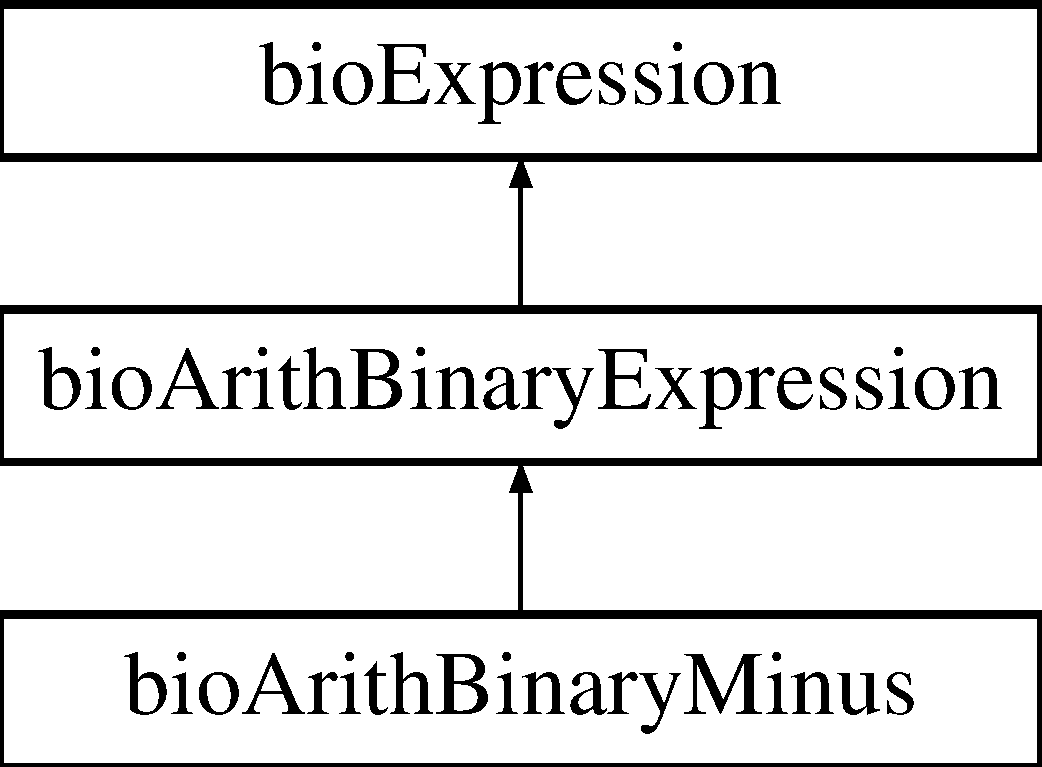
\includegraphics[height=3.000000cm]{classbio_arith_binary_minus}
\end{center}
\end{figure}
\subsection*{Public Member Functions}
\begin{DoxyCompactItemize}
\item 
\mbox{\Hypertarget{classbio_arith_binary_minus_ae67eeb46184512f95d09c2d06613db40}\label{classbio_arith_binary_minus_ae67eeb46184512f95d09c2d06613db40}} 
{\bfseries bio\+Arith\+Binary\+Minus} (\hyperlink{classbio_expression_repository}{bio\+Expression\+Repository} $\ast$rep, pat\+U\+Long par, pat\+U\+Long left, pat\+U\+Long right, pat\+Error $\ast$\&err)
\item 
virtual pat\+String \hyperlink{classbio_arith_binary_minus_a899f710bd1ba441724b9e6d7b904aa88}{get\+Operator\+Name} () const
\item 
virtual pat\+Real \hyperlink{classbio_arith_binary_minus_a0a30a984e72adb63304f75c0c53552f9}{get\+Value} (pat\+Boolean prepare\+Gradient, pat\+U\+Long current\+Lap, pat\+Error $\ast$\&err)
\item 
virtual \hyperlink{classbio_expression}{bio\+Expression} $\ast$ \hyperlink{classbio_arith_binary_minus_a7ccf12cccc95f788423753e7f61fa64f}{get\+Derivative} (pat\+U\+Long a\+Literal\+Id, pat\+Error $\ast$\&err) const
\item 
virtual \hyperlink{classbio_arith_binary_minus}{bio\+Arith\+Binary\+Minus} $\ast$ \hyperlink{classbio_arith_binary_minus_af749ca839d3194cb7bdbf5407d2bb94b}{get\+Deep\+Copy} (\hyperlink{classbio_expression_repository}{bio\+Expression\+Repository} $\ast$rep, pat\+Error $\ast$\&err) const
\item 
virtual \hyperlink{classbio_arith_binary_minus}{bio\+Arith\+Binary\+Minus} $\ast$ \hyperlink{classbio_arith_binary_minus_a93db7cf10d0bdabd9c2b89544d767e6c}{get\+Shallow\+Copy} (\hyperlink{classbio_expression_repository}{bio\+Expression\+Repository} $\ast$rep, pat\+Error $\ast$\&err) const
\item 
virtual pat\+String \hyperlink{classbio_arith_binary_minus_abfcff7ef3048216027a44af8af40471e}{get\+Expression\+String} () const
\item 
virtual \hyperlink{classbio_function_and_derivatives}{bio\+Function\+And\+Derivatives} $\ast$ \hyperlink{classbio_arith_binary_minus_a647d9b7b5fd8d5154eeba376a11d2a27}{get\+Numerical\+Function\+And\+Gradient} (vector$<$ pat\+U\+Long $>$ literal\+Ids, pat\+Boolean compute\+Hessian, pat\+Boolean debug\+Derivatives, pat\+Error $\ast$\&err)
\end{DoxyCompactItemize}
\subsection*{Additional Inherited Members}


\subsection{Detailed Description}
Class implementing a node for a soustraction operation 

\subsection{Member Function Documentation}
\mbox{\Hypertarget{classbio_arith_binary_minus_af749ca839d3194cb7bdbf5407d2bb94b}\label{classbio_arith_binary_minus_af749ca839d3194cb7bdbf5407d2bb94b}} 
\index{bio\+Arith\+Binary\+Minus@{bio\+Arith\+Binary\+Minus}!get\+Deep\+Copy@{get\+Deep\+Copy}}
\index{get\+Deep\+Copy@{get\+Deep\+Copy}!bio\+Arith\+Binary\+Minus@{bio\+Arith\+Binary\+Minus}}
\subsubsection{\texorpdfstring{get\+Deep\+Copy()}{getDeepCopy()}}
{\footnotesize\ttfamily \hyperlink{classbio_arith_binary_minus}{bio\+Arith\+Binary\+Minus} $\ast$ bio\+Arith\+Binary\+Minus\+::get\+Deep\+Copy (\begin{DoxyParamCaption}\item[{\hyperlink{classbio_expression_repository}{bio\+Expression\+Repository} $\ast$}]{rep,  }\item[{pat\+Error $\ast$\&}]{err }\end{DoxyParamCaption}) const\hspace{0.3cm}{\ttfamily [virtual]}}

Create a deep copy of the expression and returns a pointer to it. It means that new instances of the children are created. 

Reimplemented from \hyperlink{classbio_expression_a4ee1b8add634078a02eaae26cd40dcc8}{bio\+Expression}.

\mbox{\Hypertarget{classbio_arith_binary_minus_a7ccf12cccc95f788423753e7f61fa64f}\label{classbio_arith_binary_minus_a7ccf12cccc95f788423753e7f61fa64f}} 
\index{bio\+Arith\+Binary\+Minus@{bio\+Arith\+Binary\+Minus}!get\+Derivative@{get\+Derivative}}
\index{get\+Derivative@{get\+Derivative}!bio\+Arith\+Binary\+Minus@{bio\+Arith\+Binary\+Minus}}
\subsubsection{\texorpdfstring{get\+Derivative()}{getDerivative()}}
{\footnotesize\ttfamily \hyperlink{classbio_expression}{bio\+Expression} $\ast$ bio\+Arith\+Binary\+Minus\+::get\+Derivative (\begin{DoxyParamCaption}\item[{pat\+U\+Long}]{a\+Literal\+Id,  }\item[{pat\+Error $\ast$\&}]{err }\end{DoxyParamCaption}) const\hspace{0.3cm}{\ttfamily [virtual]}}

\begin{DoxyReturn}{Returns}
value of the derivative w.\+r.\+t literal 
\end{DoxyReturn}

\begin{DoxyParams}{Parameters}
{\em index} & of the literal involved in the derivative \\
\hline
{\em err} & ref. of the pointer to the error object. \\
\hline
\end{DoxyParams}


Reimplemented from \hyperlink{classbio_expression_a5915579d1193f25f216c1e273c97f2ce}{bio\+Expression}.

\mbox{\Hypertarget{classbio_arith_binary_minus_abfcff7ef3048216027a44af8af40471e}\label{classbio_arith_binary_minus_abfcff7ef3048216027a44af8af40471e}} 
\index{bio\+Arith\+Binary\+Minus@{bio\+Arith\+Binary\+Minus}!get\+Expression\+String@{get\+Expression\+String}}
\index{get\+Expression\+String@{get\+Expression\+String}!bio\+Arith\+Binary\+Minus@{bio\+Arith\+Binary\+Minus}}
\subsubsection{\texorpdfstring{get\+Expression\+String()}{getExpressionString()}}
{\footnotesize\ttfamily pat\+String bio\+Arith\+Binary\+Minus\+::get\+Expression\+String (\begin{DoxyParamCaption}{ }\end{DoxyParamCaption}) const\hspace{0.3cm}{\ttfamily [virtual]}}

Compute a string that represents the expression. It is designed to replace the expression itself when used only for comparison purposes. Code\+: +\{expr1\}\{expr2\}\+: binary plus -\/\{expr1\}\{expr2\}\+: binary minus \{expr1\}\{expr2\}\+: multiplication /\{expr1\}\{expr2\}\+: division $^\wedge$\{expr1\}\{expr2\}\+: power \&\{expr1\}\{expr2\}\+: and $\vert$\{expr1\}\{expr2\}\+: or =\{expr1\}\{expr2\}\+: equal !=\{expr1\}\{expr2\}\+: not equal $<$\{expr1\}\{expr2\}\+: lesser than $<$=\{expr1\}\{expr2\}\+: lesser or equal to $>$\{expr1\}\{expr2\}\+: greater than $>$=\{expr1\}\{expr2\}\+: greater or equal to \$A\{expr\}\+: abs \$D\mbox{[}expr\mbox{]}\mbox{[}\{expr1\}...\{exprN\}\mbox{]}\+: dictionary (\hyperlink{classbio_arith_elem}{bio\+Arith\+Elem}) \$E\{expr\}\+: exp \$L\{expr\}\+: log \$M\{expr\}\+: Unary minus \$\+Piterator\+\_\+name\{expr\}\+: prod \$Q\{string1\}\{string2\}\+: sequence \$\+Siterator\+\_\+name\{expr\}\+: sum \$\+Ziterator\+\_\+name\mbox{[}\{expr1\}...\{exprN\}\mbox{]}\+: merged sum \{expr1\}\{expr2\}...\{exprN\}//\+: list of expressions number\+: constant \#id\+: literal \&id\+: random 

Reimplemented from \hyperlink{classbio_expression_a3e4b4dca58dbbc6f0e411b30eb3f60b4}{bio\+Expression}.

\mbox{\Hypertarget{classbio_arith_binary_minus_a647d9b7b5fd8d5154eeba376a11d2a27}\label{classbio_arith_binary_minus_a647d9b7b5fd8d5154eeba376a11d2a27}} 
\index{bio\+Arith\+Binary\+Minus@{bio\+Arith\+Binary\+Minus}!get\+Numerical\+Function\+And\+Gradient@{get\+Numerical\+Function\+And\+Gradient}}
\index{get\+Numerical\+Function\+And\+Gradient@{get\+Numerical\+Function\+And\+Gradient}!bio\+Arith\+Binary\+Minus@{bio\+Arith\+Binary\+Minus}}
\subsubsection{\texorpdfstring{get\+Numerical\+Function\+And\+Gradient()}{getNumericalFunctionAndGradient()}}
{\footnotesize\ttfamily \hyperlink{classbio_function_and_derivatives}{bio\+Function\+And\+Derivatives} $\ast$ bio\+Arith\+Binary\+Minus\+::get\+Numerical\+Function\+And\+Gradient (\begin{DoxyParamCaption}\item[{vector$<$ pat\+U\+Long $>$}]{literal\+Ids,  }\item[{pat\+Boolean}]{compute\+Hessian,  }\item[{pat\+Boolean}]{debug\+Derivatives,  }\item[{pat\+Error $\ast$\&}]{err }\end{DoxyParamCaption})\hspace{0.3cm}{\ttfamily [virtual]}}

\begin{DoxyReturn}{Returns}
value and gradient of the expression 
\end{DoxyReturn}

\begin{DoxyParams}{Parameters}
{\em err} & ref. of the pointer to the error object. \\
\hline
\end{DoxyParams}


Reimplemented from \hyperlink{classbio_expression_a91c81ce80c9e972c913b10f5f3c1ed13}{bio\+Expression}.

\mbox{\Hypertarget{classbio_arith_binary_minus_a899f710bd1ba441724b9e6d7b904aa88}\label{classbio_arith_binary_minus_a899f710bd1ba441724b9e6d7b904aa88}} 
\index{bio\+Arith\+Binary\+Minus@{bio\+Arith\+Binary\+Minus}!get\+Operator\+Name@{get\+Operator\+Name}}
\index{get\+Operator\+Name@{get\+Operator\+Name}!bio\+Arith\+Binary\+Minus@{bio\+Arith\+Binary\+Minus}}
\subsubsection{\texorpdfstring{get\+Operator\+Name()}{getOperatorName()}}
{\footnotesize\ttfamily pat\+String bio\+Arith\+Binary\+Minus\+::get\+Operator\+Name (\begin{DoxyParamCaption}{ }\end{DoxyParamCaption}) const\hspace{0.3cm}{\ttfamily [virtual]}}

\begin{DoxyReturn}{Returns}
name of the operator 
\end{DoxyReturn}


Reimplemented from \hyperlink{classbio_expression_a2353a4afb3a2b0af7c63aba086a72bde}{bio\+Expression}.

\mbox{\Hypertarget{classbio_arith_binary_minus_a93db7cf10d0bdabd9c2b89544d767e6c}\label{classbio_arith_binary_minus_a93db7cf10d0bdabd9c2b89544d767e6c}} 
\index{bio\+Arith\+Binary\+Minus@{bio\+Arith\+Binary\+Minus}!get\+Shallow\+Copy@{get\+Shallow\+Copy}}
\index{get\+Shallow\+Copy@{get\+Shallow\+Copy}!bio\+Arith\+Binary\+Minus@{bio\+Arith\+Binary\+Minus}}
\subsubsection{\texorpdfstring{get\+Shallow\+Copy()}{getShallowCopy()}}
{\footnotesize\ttfamily \hyperlink{classbio_arith_binary_minus}{bio\+Arith\+Binary\+Minus} $\ast$ bio\+Arith\+Binary\+Minus\+::get\+Shallow\+Copy (\begin{DoxyParamCaption}\item[{\hyperlink{classbio_expression_repository}{bio\+Expression\+Repository} $\ast$}]{rep,  }\item[{pat\+Error $\ast$\&}]{err }\end{DoxyParamCaption}) const\hspace{0.3cm}{\ttfamily [virtual]}}

Create a shallow copy of the expression and returns a pointer to it. It means that no new instance of the children are created. It is typically called by the repository 

Reimplemented from \hyperlink{classbio_expression_a442534762693b92baaf33928979a1bf8}{bio\+Expression}.

\mbox{\Hypertarget{classbio_arith_binary_minus_a0a30a984e72adb63304f75c0c53552f9}\label{classbio_arith_binary_minus_a0a30a984e72adb63304f75c0c53552f9}} 
\index{bio\+Arith\+Binary\+Minus@{bio\+Arith\+Binary\+Minus}!get\+Value@{get\+Value}}
\index{get\+Value@{get\+Value}!bio\+Arith\+Binary\+Minus@{bio\+Arith\+Binary\+Minus}}
\subsubsection{\texorpdfstring{get\+Value()}{getValue()}}
{\footnotesize\ttfamily pat\+Real bio\+Arith\+Binary\+Minus\+::get\+Value (\begin{DoxyParamCaption}\item[{pat\+Boolean}]{prepare\+Gradient,  }\item[{pat\+U\+Long}]{current\+Lap,  }\item[{pat\+Error $\ast$\&}]{err }\end{DoxyParamCaption})\hspace{0.3cm}{\ttfamily [virtual]}}

\begin{DoxyReturn}{Returns}
value of the expression 
\end{DoxyReturn}

\begin{DoxyParams}{Parameters}
{\em err} & ref. of the pointer to the error object. \\
\hline
\end{DoxyParams}


Reimplemented from \hyperlink{classbio_expression_af58662a5d4d456f15bc4f2c9bd4f8a5b}{bio\+Expression}.



The documentation for this class was generated from the following files\+:\begin{DoxyCompactItemize}
\item 
bio\+Arith\+Binary\+Minus.\+h\item 
bio\+Arith\+Binary\+Minus.\+cc\end{DoxyCompactItemize}

\hypertarget{classbio_arith_binary_plus}{}\section{bio\+Arith\+Binary\+Plus Class Reference}
\label{classbio_arith_binary_plus}\index{bio\+Arith\+Binary\+Plus@{bio\+Arith\+Binary\+Plus}}


{\ttfamily \#include $<$bio\+Arith\+Binary\+Plus.\+h$>$}

Inheritance diagram for bio\+Arith\+Binary\+Plus\+:\begin{figure}[H]
\begin{center}
\leavevmode
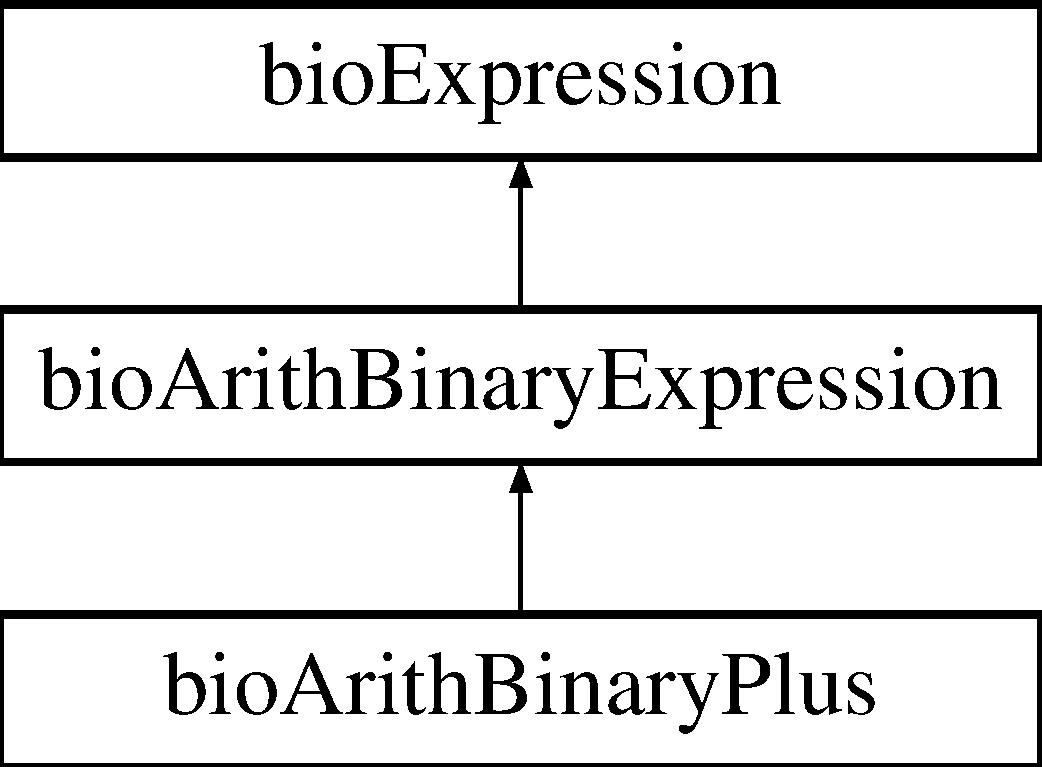
\includegraphics[height=3.000000cm]{classbio_arith_binary_plus}
\end{center}
\end{figure}
\subsection*{Public Member Functions}
\begin{DoxyCompactItemize}
\item 
\mbox{\Hypertarget{classbio_arith_binary_plus_a4b93682b80f1fa98f88679e1cbd6684b}\label{classbio_arith_binary_plus_a4b93682b80f1fa98f88679e1cbd6684b}} 
{\bfseries bio\+Arith\+Binary\+Plus} (\hyperlink{classbio_expression_repository}{bio\+Expression\+Repository} $\ast$rep, pat\+U\+Long par, pat\+U\+Long left, pat\+U\+Long right, pat\+Error $\ast$\&err)
\item 
virtual pat\+String \hyperlink{classbio_arith_binary_plus_a1d9032fda00f9f0d00f3244714c35cdb}{get\+Operator\+Name} () const
\item 
virtual pat\+Real \hyperlink{classbio_arith_binary_plus_a40a7b6945cd9118f110e580ab90c7b5f}{get\+Value} (pat\+Boolean prepare\+Gradient, pat\+U\+Long current\+Lap, pat\+Error $\ast$\&err)
\item 
virtual \hyperlink{classbio_expression}{bio\+Expression} $\ast$ \hyperlink{classbio_arith_binary_plus_a790383068d3be59378a18206199fb3f1}{get\+Derivative} (pat\+U\+Long a\+Literal\+Id, pat\+Error $\ast$\&err) const
\item 
virtual \hyperlink{classbio_arith_binary_plus}{bio\+Arith\+Binary\+Plus} $\ast$ \hyperlink{classbio_arith_binary_plus_a5ec101b24a6b02bb3fb19803749b3e83}{get\+Deep\+Copy} (\hyperlink{classbio_expression_repository}{bio\+Expression\+Repository} $\ast$rep, pat\+Error $\ast$\&err) const
\item 
virtual \hyperlink{classbio_arith_binary_plus}{bio\+Arith\+Binary\+Plus} $\ast$ \hyperlink{classbio_arith_binary_plus_a4e2587ad009e65821632b18d0253ff4c}{get\+Shallow\+Copy} (\hyperlink{classbio_expression_repository}{bio\+Expression\+Repository} $\ast$rep, pat\+Error $\ast$\&err) const
\item 
virtual pat\+String \hyperlink{classbio_arith_binary_plus_afb38f58cc62bf6fbce4383ce40b1aecf}{get\+Expression} (pat\+Error $\ast$\&err) const
\item 
virtual pat\+String \hyperlink{classbio_arith_binary_plus_af062d1a1394e9fedf99e23911110f384}{get\+Expression\+String} () const
\item 
virtual \hyperlink{classbio_function_and_derivatives}{bio\+Function\+And\+Derivatives} $\ast$ \hyperlink{classbio_arith_binary_plus_a17d6b61d7dd58d5c03c087ddc7054632}{get\+Numerical\+Function\+And\+Gradient} (vector$<$ pat\+U\+Long $>$ literal\+Ids, pat\+Boolean compute\+Hessian, pat\+Boolean debug\+Derivatives, pat\+Error $\ast$\&err)
\end{DoxyCompactItemize}
\subsection*{Additional Inherited Members}


\subsection{Detailed Description}
Class implementing a node for an addition operation 

\subsection{Member Function Documentation}
\mbox{\Hypertarget{classbio_arith_binary_plus_a5ec101b24a6b02bb3fb19803749b3e83}\label{classbio_arith_binary_plus_a5ec101b24a6b02bb3fb19803749b3e83}} 
\index{bio\+Arith\+Binary\+Plus@{bio\+Arith\+Binary\+Plus}!get\+Deep\+Copy@{get\+Deep\+Copy}}
\index{get\+Deep\+Copy@{get\+Deep\+Copy}!bio\+Arith\+Binary\+Plus@{bio\+Arith\+Binary\+Plus}}
\subsubsection{\texorpdfstring{get\+Deep\+Copy()}{getDeepCopy()}}
{\footnotesize\ttfamily \hyperlink{classbio_arith_binary_plus}{bio\+Arith\+Binary\+Plus} $\ast$ bio\+Arith\+Binary\+Plus\+::get\+Deep\+Copy (\begin{DoxyParamCaption}\item[{\hyperlink{classbio_expression_repository}{bio\+Expression\+Repository} $\ast$}]{rep,  }\item[{pat\+Error $\ast$\&}]{err }\end{DoxyParamCaption}) const\hspace{0.3cm}{\ttfamily [virtual]}}

Create a deep copy of the expression and returns a pointer to it. It means that new instances of the children are created. 

Reimplemented from \hyperlink{classbio_expression_a4ee1b8add634078a02eaae26cd40dcc8}{bio\+Expression}.

\mbox{\Hypertarget{classbio_arith_binary_plus_a790383068d3be59378a18206199fb3f1}\label{classbio_arith_binary_plus_a790383068d3be59378a18206199fb3f1}} 
\index{bio\+Arith\+Binary\+Plus@{bio\+Arith\+Binary\+Plus}!get\+Derivative@{get\+Derivative}}
\index{get\+Derivative@{get\+Derivative}!bio\+Arith\+Binary\+Plus@{bio\+Arith\+Binary\+Plus}}
\subsubsection{\texorpdfstring{get\+Derivative()}{getDerivative()}}
{\footnotesize\ttfamily \hyperlink{classbio_expression}{bio\+Expression} $\ast$ bio\+Arith\+Binary\+Plus\+::get\+Derivative (\begin{DoxyParamCaption}\item[{pat\+U\+Long}]{a\+Literal\+Id,  }\item[{pat\+Error $\ast$\&}]{err }\end{DoxyParamCaption}) const\hspace{0.3cm}{\ttfamily [virtual]}}

\begin{DoxyReturn}{Returns}
value of the derivative w.\+r.\+t literal 
\end{DoxyReturn}

\begin{DoxyParams}{Parameters}
{\em index} & of the literal involved in the derivative \\
\hline
{\em err} & ref. of the pointer to the error object. \\
\hline
\end{DoxyParams}


Reimplemented from \hyperlink{classbio_expression_a5915579d1193f25f216c1e273c97f2ce}{bio\+Expression}.

\mbox{\Hypertarget{classbio_arith_binary_plus_afb38f58cc62bf6fbce4383ce40b1aecf}\label{classbio_arith_binary_plus_afb38f58cc62bf6fbce4383ce40b1aecf}} 
\index{bio\+Arith\+Binary\+Plus@{bio\+Arith\+Binary\+Plus}!get\+Expression@{get\+Expression}}
\index{get\+Expression@{get\+Expression}!bio\+Arith\+Binary\+Plus@{bio\+Arith\+Binary\+Plus}}
\subsubsection{\texorpdfstring{get\+Expression()}{getExpression()}}
{\footnotesize\ttfamily pat\+String bio\+Arith\+Binary\+Plus\+::get\+Expression (\begin{DoxyParamCaption}\item[{pat\+Error $\ast$\&}]{err }\end{DoxyParamCaption}) const\hspace{0.3cm}{\ttfamily [virtual]}}

\begin{DoxyReturn}{Returns}
printed expression 
\end{DoxyReturn}


Reimplemented from \hyperlink{classbio_arith_binary_expression_a6c48d0f1c7b6ba1b8cf3910b9ad04f93}{bio\+Arith\+Binary\+Expression}.

\mbox{\Hypertarget{classbio_arith_binary_plus_af062d1a1394e9fedf99e23911110f384}\label{classbio_arith_binary_plus_af062d1a1394e9fedf99e23911110f384}} 
\index{bio\+Arith\+Binary\+Plus@{bio\+Arith\+Binary\+Plus}!get\+Expression\+String@{get\+Expression\+String}}
\index{get\+Expression\+String@{get\+Expression\+String}!bio\+Arith\+Binary\+Plus@{bio\+Arith\+Binary\+Plus}}
\subsubsection{\texorpdfstring{get\+Expression\+String()}{getExpressionString()}}
{\footnotesize\ttfamily pat\+String bio\+Arith\+Binary\+Plus\+::get\+Expression\+String (\begin{DoxyParamCaption}{ }\end{DoxyParamCaption}) const\hspace{0.3cm}{\ttfamily [virtual]}}

Compute a string that represents the expression. It is designed to replace the expression itself when used only for comparison purposes. Code\+: +\{expr1\}\{expr2\}\+: binary plus -\/\{expr1\}\{expr2\}\+: binary minus \{expr1\}\{expr2\}\+: multiplication /\{expr1\}\{expr2\}\+: division $^\wedge$\{expr1\}\{expr2\}\+: power \&\{expr1\}\{expr2\}\+: and $\vert$\{expr1\}\{expr2\}\+: or =\{expr1\}\{expr2\}\+: equal !=\{expr1\}\{expr2\}\+: not equal $<$\{expr1\}\{expr2\}\+: lesser than $<$=\{expr1\}\{expr2\}\+: lesser or equal to $>$\{expr1\}\{expr2\}\+: greater than $>$=\{expr1\}\{expr2\}\+: greater or equal to \$A\{expr\}\+: abs \$D\mbox{[}expr\mbox{]}\mbox{[}\{expr1\}...\{exprN\}\mbox{]}\+: dictionary (\hyperlink{classbio_arith_elem}{bio\+Arith\+Elem}) \$E\{expr\}\+: exp \$L\{expr\}\+: log \$M\{expr\}\+: Unary minus \$\+Piterator\+\_\+name\{expr\}\+: prod \$Q\{string1\}\{string2\}\+: sequence \$\+Siterator\+\_\+name\{expr\}\+: sum \$\+Ziterator\+\_\+name\mbox{[}\{expr1\}...\{exprN\}\mbox{]}\+: merged sum \{expr1\}\{expr2\}...\{exprN\}//\+: list of expressions number\+: constant \#id\+: literal \&id\+: random 

Reimplemented from \hyperlink{classbio_expression_a3e4b4dca58dbbc6f0e411b30eb3f60b4}{bio\+Expression}.

\mbox{\Hypertarget{classbio_arith_binary_plus_a17d6b61d7dd58d5c03c087ddc7054632}\label{classbio_arith_binary_plus_a17d6b61d7dd58d5c03c087ddc7054632}} 
\index{bio\+Arith\+Binary\+Plus@{bio\+Arith\+Binary\+Plus}!get\+Numerical\+Function\+And\+Gradient@{get\+Numerical\+Function\+And\+Gradient}}
\index{get\+Numerical\+Function\+And\+Gradient@{get\+Numerical\+Function\+And\+Gradient}!bio\+Arith\+Binary\+Plus@{bio\+Arith\+Binary\+Plus}}
\subsubsection{\texorpdfstring{get\+Numerical\+Function\+And\+Gradient()}{getNumericalFunctionAndGradient()}}
{\footnotesize\ttfamily \hyperlink{classbio_function_and_derivatives}{bio\+Function\+And\+Derivatives} $\ast$ bio\+Arith\+Binary\+Plus\+::get\+Numerical\+Function\+And\+Gradient (\begin{DoxyParamCaption}\item[{vector$<$ pat\+U\+Long $>$}]{literal\+Ids,  }\item[{pat\+Boolean}]{compute\+Hessian,  }\item[{pat\+Boolean}]{debug\+Derivatives,  }\item[{pat\+Error $\ast$\&}]{err }\end{DoxyParamCaption})\hspace{0.3cm}{\ttfamily [virtual]}}

\begin{DoxyReturn}{Returns}
value and gradient of the expression 
\end{DoxyReturn}

\begin{DoxyParams}{Parameters}
{\em err} & ref. of the pointer to the error object. \\
\hline
\end{DoxyParams}


Reimplemented from \hyperlink{classbio_expression_a91c81ce80c9e972c913b10f5f3c1ed13}{bio\+Expression}.

\mbox{\Hypertarget{classbio_arith_binary_plus_a1d9032fda00f9f0d00f3244714c35cdb}\label{classbio_arith_binary_plus_a1d9032fda00f9f0d00f3244714c35cdb}} 
\index{bio\+Arith\+Binary\+Plus@{bio\+Arith\+Binary\+Plus}!get\+Operator\+Name@{get\+Operator\+Name}}
\index{get\+Operator\+Name@{get\+Operator\+Name}!bio\+Arith\+Binary\+Plus@{bio\+Arith\+Binary\+Plus}}
\subsubsection{\texorpdfstring{get\+Operator\+Name()}{getOperatorName()}}
{\footnotesize\ttfamily pat\+String bio\+Arith\+Binary\+Plus\+::get\+Operator\+Name (\begin{DoxyParamCaption}{ }\end{DoxyParamCaption}) const\hspace{0.3cm}{\ttfamily [virtual]}}

\begin{DoxyReturn}{Returns}
name of the operator 
\end{DoxyReturn}


Reimplemented from \hyperlink{classbio_expression_a2353a4afb3a2b0af7c63aba086a72bde}{bio\+Expression}.

\mbox{\Hypertarget{classbio_arith_binary_plus_a4e2587ad009e65821632b18d0253ff4c}\label{classbio_arith_binary_plus_a4e2587ad009e65821632b18d0253ff4c}} 
\index{bio\+Arith\+Binary\+Plus@{bio\+Arith\+Binary\+Plus}!get\+Shallow\+Copy@{get\+Shallow\+Copy}}
\index{get\+Shallow\+Copy@{get\+Shallow\+Copy}!bio\+Arith\+Binary\+Plus@{bio\+Arith\+Binary\+Plus}}
\subsubsection{\texorpdfstring{get\+Shallow\+Copy()}{getShallowCopy()}}
{\footnotesize\ttfamily \hyperlink{classbio_arith_binary_plus}{bio\+Arith\+Binary\+Plus} $\ast$ bio\+Arith\+Binary\+Plus\+::get\+Shallow\+Copy (\begin{DoxyParamCaption}\item[{\hyperlink{classbio_expression_repository}{bio\+Expression\+Repository} $\ast$}]{rep,  }\item[{pat\+Error $\ast$\&}]{err }\end{DoxyParamCaption}) const\hspace{0.3cm}{\ttfamily [virtual]}}

Create a shallow copy of the expression and returns a pointer to it. It means that no new instance of the children are created. It is typically called by the repository 

Reimplemented from \hyperlink{classbio_expression_a442534762693b92baaf33928979a1bf8}{bio\+Expression}.

\mbox{\Hypertarget{classbio_arith_binary_plus_a40a7b6945cd9118f110e580ab90c7b5f}\label{classbio_arith_binary_plus_a40a7b6945cd9118f110e580ab90c7b5f}} 
\index{bio\+Arith\+Binary\+Plus@{bio\+Arith\+Binary\+Plus}!get\+Value@{get\+Value}}
\index{get\+Value@{get\+Value}!bio\+Arith\+Binary\+Plus@{bio\+Arith\+Binary\+Plus}}
\subsubsection{\texorpdfstring{get\+Value()}{getValue()}}
{\footnotesize\ttfamily pat\+Real bio\+Arith\+Binary\+Plus\+::get\+Value (\begin{DoxyParamCaption}\item[{pat\+Boolean}]{prepare\+Gradient,  }\item[{pat\+U\+Long}]{current\+Lap,  }\item[{pat\+Error $\ast$\&}]{err }\end{DoxyParamCaption})\hspace{0.3cm}{\ttfamily [virtual]}}

\begin{DoxyReturn}{Returns}
value of the expression 
\end{DoxyReturn}

\begin{DoxyParams}{Parameters}
{\em err} & ref. of the pointer to the error object. \\
\hline
\end{DoxyParams}


Reimplemented from \hyperlink{classbio_expression_af58662a5d4d456f15bc4f2c9bd4f8a5b}{bio\+Expression}.



The documentation for this class was generated from the following files\+:\begin{DoxyCompactItemize}
\item 
bio\+Arith\+Binary\+Plus.\+h\item 
bio\+Arith\+Binary\+Plus.\+cc\end{DoxyCompactItemize}

\hypertarget{classbio_arith_composite_literal}{}\section{bio\+Arith\+Composite\+Literal Class Reference}
\label{classbio_arith_composite_literal}\index{bio\+Arith\+Composite\+Literal@{bio\+Arith\+Composite\+Literal}}


{\ttfamily \#include $<$bio\+Arith\+Composite\+Literal.\+h$>$}

Inheritance diagram for bio\+Arith\+Composite\+Literal\+:\begin{figure}[H]
\begin{center}
\leavevmode
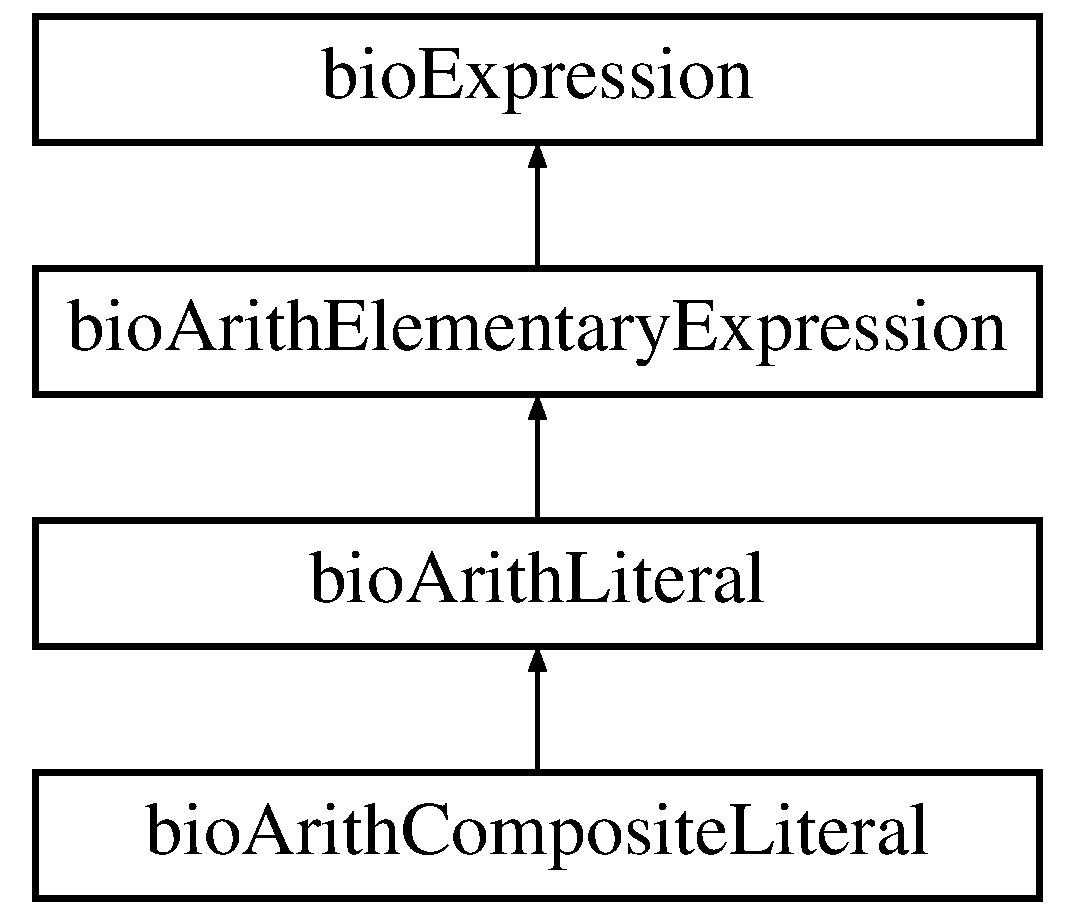
\includegraphics[height=4.000000cm]{classbio_arith_composite_literal}
\end{center}
\end{figure}
\subsection*{Public Member Functions}
\begin{DoxyCompactItemize}
\item 
virtual \hyperlink{classbio_arith_composite_literal}{bio\+Arith\+Composite\+Literal} $\ast$ \hyperlink{classbio_arith_composite_literal_aff5a7801055d4691dcc1ee84cc9fa201}{get\+Deep\+Copy} (\hyperlink{classbio_expression_repository}{bio\+Expression\+Repository} $\ast$rep, pat\+Error $\ast$\&err) const
\item 
virtual \hyperlink{classbio_arith_composite_literal}{bio\+Arith\+Composite\+Literal} $\ast$ \hyperlink{classbio_arith_composite_literal_a99216fa86facca3b310a985c69116136}{get\+Shallow\+Copy} (\hyperlink{classbio_expression_repository}{bio\+Expression\+Repository} $\ast$rep, pat\+Error $\ast$\&err) const
\item 
virtual pat\+Real \hyperlink{classbio_arith_composite_literal_ab0471105a849e772c1e93f5b45b66acb}{get\+Value} (pat\+Boolean prepare\+Gradient, pat\+U\+Long current\+Lap, pat\+Error $\ast$\&err)
\end{DoxyCompactItemize}
\subsection*{Protected Attributes}
\begin{DoxyCompactItemize}
\item 
\mbox{\Hypertarget{classbio_arith_composite_literal_a2532b2dd05d30e3cbcb7f3051d1b90b6}\label{classbio_arith_composite_literal_a2532b2dd05d30e3cbcb7f3051d1b90b6}} 
pat\+U\+Long {\bfseries the\+Composite\+Literal\+Id}
\end{DoxyCompactItemize}


\subsection{Detailed Description}
Class implementing the node for composite literals in an expression 

\subsection{Member Function Documentation}
\mbox{\Hypertarget{classbio_arith_composite_literal_aff5a7801055d4691dcc1ee84cc9fa201}\label{classbio_arith_composite_literal_aff5a7801055d4691dcc1ee84cc9fa201}} 
\index{bio\+Arith\+Composite\+Literal@{bio\+Arith\+Composite\+Literal}!get\+Deep\+Copy@{get\+Deep\+Copy}}
\index{get\+Deep\+Copy@{get\+Deep\+Copy}!bio\+Arith\+Composite\+Literal@{bio\+Arith\+Composite\+Literal}}
\subsubsection{\texorpdfstring{get\+Deep\+Copy()}{getDeepCopy()}}
{\footnotesize\ttfamily \hyperlink{classbio_arith_composite_literal}{bio\+Arith\+Composite\+Literal} $\ast$ bio\+Arith\+Composite\+Literal\+::get\+Deep\+Copy (\begin{DoxyParamCaption}\item[{\hyperlink{classbio_expression_repository}{bio\+Expression\+Repository} $\ast$}]{rep,  }\item[{pat\+Error $\ast$\&}]{err }\end{DoxyParamCaption}) const\hspace{0.3cm}{\ttfamily [virtual]}}

Create a deep copy of the expression and returns a pointer to it. It means that new instances of the children are created. 

Reimplemented from \hyperlink{classbio_expression_a4ee1b8add634078a02eaae26cd40dcc8}{bio\+Expression}.

\mbox{\Hypertarget{classbio_arith_composite_literal_a99216fa86facca3b310a985c69116136}\label{classbio_arith_composite_literal_a99216fa86facca3b310a985c69116136}} 
\index{bio\+Arith\+Composite\+Literal@{bio\+Arith\+Composite\+Literal}!get\+Shallow\+Copy@{get\+Shallow\+Copy}}
\index{get\+Shallow\+Copy@{get\+Shallow\+Copy}!bio\+Arith\+Composite\+Literal@{bio\+Arith\+Composite\+Literal}}
\subsubsection{\texorpdfstring{get\+Shallow\+Copy()}{getShallowCopy()}}
{\footnotesize\ttfamily \hyperlink{classbio_arith_composite_literal}{bio\+Arith\+Composite\+Literal} $\ast$ bio\+Arith\+Composite\+Literal\+::get\+Shallow\+Copy (\begin{DoxyParamCaption}\item[{\hyperlink{classbio_expression_repository}{bio\+Expression\+Repository} $\ast$}]{rep,  }\item[{pat\+Error $\ast$\&}]{err }\end{DoxyParamCaption}) const\hspace{0.3cm}{\ttfamily [virtual]}}

Create a shallow copy of the expression and returns a pointer to it. It means that no new instance of the children are created. It is typically called by the repository 

Reimplemented from \hyperlink{classbio_expression_a442534762693b92baaf33928979a1bf8}{bio\+Expression}.

\mbox{\Hypertarget{classbio_arith_composite_literal_ab0471105a849e772c1e93f5b45b66acb}\label{classbio_arith_composite_literal_ab0471105a849e772c1e93f5b45b66acb}} 
\index{bio\+Arith\+Composite\+Literal@{bio\+Arith\+Composite\+Literal}!get\+Value@{get\+Value}}
\index{get\+Value@{get\+Value}!bio\+Arith\+Composite\+Literal@{bio\+Arith\+Composite\+Literal}}
\subsubsection{\texorpdfstring{get\+Value()}{getValue()}}
{\footnotesize\ttfamily pat\+Real bio\+Arith\+Composite\+Literal\+::get\+Value (\begin{DoxyParamCaption}\item[{pat\+Boolean}]{prepare\+Gradient,  }\item[{pat\+U\+Long}]{current\+Lap,  }\item[{pat\+Error $\ast$\&}]{err }\end{DoxyParamCaption})\hspace{0.3cm}{\ttfamily [virtual]}}

\begin{DoxyReturn}{Returns}
value of the expression 
\end{DoxyReturn}

\begin{DoxyParams}{Parameters}
{\em err} & ref. of the pointer to the error object. \\
\hline
\end{DoxyParams}


Reimplemented from \hyperlink{classbio_expression_af58662a5d4d456f15bc4f2c9bd4f8a5b}{bio\+Expression}.



The documentation for this class was generated from the following files\+:\begin{DoxyCompactItemize}
\item 
bio\+Arith\+Composite\+Literal.\+h\item 
bio\+Arith\+Composite\+Literal.\+cc\end{DoxyCompactItemize}

\hypertarget{classbio_arith_constant}{}\section{bio\+Arith\+Constant Class Reference}
\label{classbio_arith_constant}\index{bio\+Arith\+Constant@{bio\+Arith\+Constant}}


{\ttfamily \#include $<$bio\+Arith\+Constant.\+h$>$}

Inheritance diagram for bio\+Arith\+Constant\+:\begin{figure}[H]
\begin{center}
\leavevmode
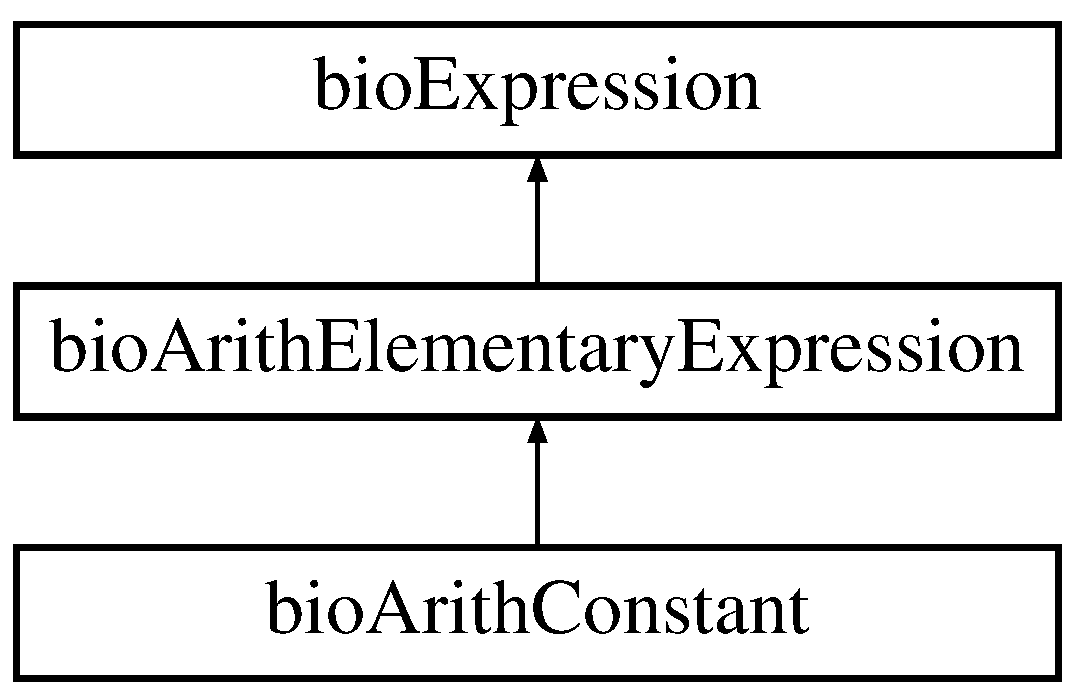
\includegraphics[height=3.000000cm]{classbio_arith_constant}
\end{center}
\end{figure}
\subsection*{Public Member Functions}
\begin{DoxyCompactItemize}
\item 
\mbox{\Hypertarget{classbio_arith_constant_adab97ecd417c13ba7d839a93fde5d135}\label{classbio_arith_constant_adab97ecd417c13ba7d839a93fde5d135}} 
{\bfseries bio\+Arith\+Constant} (\hyperlink{classbio_expression_repository}{bio\+Expression\+Repository} $\ast$rep, pat\+U\+Long par, pat\+Real a\+Value)
\item 
virtual pat\+String \hyperlink{classbio_arith_constant_a13a6799f54ffbbc8b43d54b213888fe0}{get\+Operator\+Name} () const
\item 
virtual pat\+Real \hyperlink{classbio_arith_constant_a60b9f8bf637586c0464356dfcf3bc4a3}{get\+Value} (pat\+Boolean prepare\+Gradient, pat\+U\+Long current\+Lap, pat\+Error $\ast$\&err)
\item 
virtual \hyperlink{classbio_expression}{bio\+Expression} $\ast$ \hyperlink{classbio_arith_constant_afbe5eaceb8943323f7bf0bfd3491b19a}{get\+Derivative} (pat\+U\+Long a\+Literal\+Id, pat\+Error $\ast$\&err) const
\item 
virtual \hyperlink{classbio_arith_constant}{bio\+Arith\+Constant} $\ast$ \hyperlink{classbio_arith_constant_af2f4fed6a41757d2cfa06a06b4d16923}{get\+Deep\+Copy} (\hyperlink{classbio_expression_repository}{bio\+Expression\+Repository} $\ast$rep, pat\+Error $\ast$\&err) const
\item 
virtual \hyperlink{classbio_arith_constant}{bio\+Arith\+Constant} $\ast$ \hyperlink{classbio_arith_constant_a521fe691fd4efd9f93ff95a0e478148d}{get\+Shallow\+Copy} (\hyperlink{classbio_expression_repository}{bio\+Expression\+Repository} $\ast$rep, pat\+Error $\ast$\&err) const
\item 
virtual pat\+Boolean \hyperlink{classbio_arith_constant_acd4439b84514d6612a97d422ba8f60c1}{is\+Structurally\+Zero} () const
\item 
virtual pat\+Boolean \hyperlink{classbio_arith_constant_a979ab2441d612a23a708fa3c10f3dd6a}{is\+Structurally\+One} () const
\item 
\mbox{\Hypertarget{classbio_arith_constant_a6685609d7bba442f937a04f4885202df}\label{classbio_arith_constant_a6685609d7bba442f937a04f4885202df}} 
virtual pat\+Boolean {\bfseries is\+Constant} () const
\item 
virtual pat\+String \hyperlink{classbio_arith_constant_a50fd07c61fc6674c05f23345b972807c}{get\+Expression} (pat\+Error $\ast$\&err) const
\item 
virtual pat\+String \hyperlink{classbio_arith_constant_ae815cae63ba8b2807c653fc1ca343672}{get\+Expression\+String} () const
\item 
\mbox{\Hypertarget{classbio_arith_constant_a098b5439de43bf80c63415aebc4dfffc}\label{classbio_arith_constant_a098b5439de43bf80c63415aebc4dfffc}} 
virtual pat\+Boolean {\bfseries depends\+Of} (pat\+U\+Long a\+Literal\+Id) const
\item 
virtual \hyperlink{classbio_function_and_derivatives}{bio\+Function\+And\+Derivatives} $\ast$ \hyperlink{classbio_arith_constant_a42bfbc2f6dfc86d5530fee64146b2172}{get\+Numerical\+Function\+And\+Gradient} (vector$<$ pat\+U\+Long $>$ literal\+Ids, pat\+Boolean compute\+Hessian, pat\+Boolean debug\+Derivatives, pat\+Error $\ast$\&err)
\end{DoxyCompactItemize}
\subsection*{Protected Attributes}
\begin{DoxyCompactItemize}
\item 
\mbox{\Hypertarget{classbio_arith_constant_acac35d0d81e46fc992e046a3e2302edb}\label{classbio_arith_constant_acac35d0d81e46fc992e046a3e2302edb}} 
pat\+Real {\bfseries the\+Value}
\end{DoxyCompactItemize}


\subsection{Detailed Description}
Class implementing the node for numerical constants in an expression 

\subsection{Member Function Documentation}
\mbox{\Hypertarget{classbio_arith_constant_af2f4fed6a41757d2cfa06a06b4d16923}\label{classbio_arith_constant_af2f4fed6a41757d2cfa06a06b4d16923}} 
\index{bio\+Arith\+Constant@{bio\+Arith\+Constant}!get\+Deep\+Copy@{get\+Deep\+Copy}}
\index{get\+Deep\+Copy@{get\+Deep\+Copy}!bio\+Arith\+Constant@{bio\+Arith\+Constant}}
\subsubsection{\texorpdfstring{get\+Deep\+Copy()}{getDeepCopy()}}
{\footnotesize\ttfamily \hyperlink{classbio_arith_constant}{bio\+Arith\+Constant} $\ast$ bio\+Arith\+Constant\+::get\+Deep\+Copy (\begin{DoxyParamCaption}\item[{\hyperlink{classbio_expression_repository}{bio\+Expression\+Repository} $\ast$}]{rep,  }\item[{pat\+Error $\ast$\&}]{err }\end{DoxyParamCaption}) const\hspace{0.3cm}{\ttfamily [virtual]}}

Create a deep copy of the expression and returns a pointer to it. It means that new instances of the children are created. 

Reimplemented from \hyperlink{classbio_expression_a4ee1b8add634078a02eaae26cd40dcc8}{bio\+Expression}.

\mbox{\Hypertarget{classbio_arith_constant_afbe5eaceb8943323f7bf0bfd3491b19a}\label{classbio_arith_constant_afbe5eaceb8943323f7bf0bfd3491b19a}} 
\index{bio\+Arith\+Constant@{bio\+Arith\+Constant}!get\+Derivative@{get\+Derivative}}
\index{get\+Derivative@{get\+Derivative}!bio\+Arith\+Constant@{bio\+Arith\+Constant}}
\subsubsection{\texorpdfstring{get\+Derivative()}{getDerivative()}}
{\footnotesize\ttfamily \hyperlink{classbio_expression}{bio\+Expression} $\ast$ bio\+Arith\+Constant\+::get\+Derivative (\begin{DoxyParamCaption}\item[{pat\+U\+Long}]{a\+Literal\+Id,  }\item[{pat\+Error $\ast$\&}]{err }\end{DoxyParamCaption}) const\hspace{0.3cm}{\ttfamily [virtual]}}

\begin{DoxyReturn}{Returns}
value of the derivative w.\+r.\+t literal 
\end{DoxyReturn}

\begin{DoxyParams}{Parameters}
{\em index} & of the literal involved in the derivative \\
\hline
{\em err} & ref. of the pointer to the error object. \\
\hline
\end{DoxyParams}


Reimplemented from \hyperlink{classbio_expression_a5915579d1193f25f216c1e273c97f2ce}{bio\+Expression}.

\mbox{\Hypertarget{classbio_arith_constant_a50fd07c61fc6674c05f23345b972807c}\label{classbio_arith_constant_a50fd07c61fc6674c05f23345b972807c}} 
\index{bio\+Arith\+Constant@{bio\+Arith\+Constant}!get\+Expression@{get\+Expression}}
\index{get\+Expression@{get\+Expression}!bio\+Arith\+Constant@{bio\+Arith\+Constant}}
\subsubsection{\texorpdfstring{get\+Expression()}{getExpression()}}
{\footnotesize\ttfamily pat\+String bio\+Arith\+Constant\+::get\+Expression (\begin{DoxyParamCaption}\item[{pat\+Error $\ast$\&}]{err }\end{DoxyParamCaption}) const\hspace{0.3cm}{\ttfamily [virtual]}}

\begin{DoxyReturn}{Returns}
printed expression 
\end{DoxyReturn}


Reimplemented from \hyperlink{classbio_arith_elementary_expression_a9293635c83789f547b5642855f8c8f16}{bio\+Arith\+Elementary\+Expression}.

\mbox{\Hypertarget{classbio_arith_constant_ae815cae63ba8b2807c653fc1ca343672}\label{classbio_arith_constant_ae815cae63ba8b2807c653fc1ca343672}} 
\index{bio\+Arith\+Constant@{bio\+Arith\+Constant}!get\+Expression\+String@{get\+Expression\+String}}
\index{get\+Expression\+String@{get\+Expression\+String}!bio\+Arith\+Constant@{bio\+Arith\+Constant}}
\subsubsection{\texorpdfstring{get\+Expression\+String()}{getExpressionString()}}
{\footnotesize\ttfamily pat\+String bio\+Arith\+Constant\+::get\+Expression\+String (\begin{DoxyParamCaption}{ }\end{DoxyParamCaption}) const\hspace{0.3cm}{\ttfamily [virtual]}}

Compute a string that represents the expression. It is designed to replace the expression itself when used only for comparison purposes. Code\+: +\{expr1\}\{expr2\}\+: binary plus -\/\{expr1\}\{expr2\}\+: binary minus \{expr1\}\{expr2\}\+: multiplication /\{expr1\}\{expr2\}\+: division $^\wedge$\{expr1\}\{expr2\}\+: power \&\{expr1\}\{expr2\}\+: and $\vert$\{expr1\}\{expr2\}\+: or =\{expr1\}\{expr2\}\+: equal !=\{expr1\}\{expr2\}\+: not equal $<$\{expr1\}\{expr2\}\+: lesser than $<$=\{expr1\}\{expr2\}\+: lesser or equal to $>$\{expr1\}\{expr2\}\+: greater than $>$=\{expr1\}\{expr2\}\+: greater or equal to \$A\{expr\}\+: abs \$D\mbox{[}expr\mbox{]}\mbox{[}\{expr1\}...\{exprN\}\mbox{]}\+: dictionary (\hyperlink{classbio_arith_elem}{bio\+Arith\+Elem}) \$E\{expr\}\+: exp \$L\{expr\}\+: log \$M\{expr\}\+: Unary minus \$\+Piterator\+\_\+name\{expr\}\+: prod \$Q\{string1\}\{string2\}\+: sequence \$\+Siterator\+\_\+name\{expr\}\+: sum \$\+Ziterator\+\_\+name\mbox{[}\{expr1\}...\{exprN\}\mbox{]}\+: merged sum \{expr1\}\{expr2\}...\{exprN\}//\+: list of expressions number\+: constant \#id\+: literal \&id\+: random 

Reimplemented from \hyperlink{classbio_expression_a3e4b4dca58dbbc6f0e411b30eb3f60b4}{bio\+Expression}.

\mbox{\Hypertarget{classbio_arith_constant_a42bfbc2f6dfc86d5530fee64146b2172}\label{classbio_arith_constant_a42bfbc2f6dfc86d5530fee64146b2172}} 
\index{bio\+Arith\+Constant@{bio\+Arith\+Constant}!get\+Numerical\+Function\+And\+Gradient@{get\+Numerical\+Function\+And\+Gradient}}
\index{get\+Numerical\+Function\+And\+Gradient@{get\+Numerical\+Function\+And\+Gradient}!bio\+Arith\+Constant@{bio\+Arith\+Constant}}
\subsubsection{\texorpdfstring{get\+Numerical\+Function\+And\+Gradient()}{getNumericalFunctionAndGradient()}}
{\footnotesize\ttfamily \hyperlink{classbio_function_and_derivatives}{bio\+Function\+And\+Derivatives} $\ast$ bio\+Arith\+Constant\+::get\+Numerical\+Function\+And\+Gradient (\begin{DoxyParamCaption}\item[{vector$<$ pat\+U\+Long $>$}]{literal\+Ids,  }\item[{pat\+Boolean}]{compute\+Hessian,  }\item[{pat\+Boolean}]{debug\+Derivatives,  }\item[{pat\+Error $\ast$\&}]{err }\end{DoxyParamCaption})\hspace{0.3cm}{\ttfamily [virtual]}}

\begin{DoxyReturn}{Returns}
value and gradient of the expression 
\end{DoxyReturn}

\begin{DoxyParams}{Parameters}
{\em err} & ref. of the pointer to the error object. \\
\hline
\end{DoxyParams}


Reimplemented from \hyperlink{classbio_expression_a91c81ce80c9e972c913b10f5f3c1ed13}{bio\+Expression}.

\mbox{\Hypertarget{classbio_arith_constant_a13a6799f54ffbbc8b43d54b213888fe0}\label{classbio_arith_constant_a13a6799f54ffbbc8b43d54b213888fe0}} 
\index{bio\+Arith\+Constant@{bio\+Arith\+Constant}!get\+Operator\+Name@{get\+Operator\+Name}}
\index{get\+Operator\+Name@{get\+Operator\+Name}!bio\+Arith\+Constant@{bio\+Arith\+Constant}}
\subsubsection{\texorpdfstring{get\+Operator\+Name()}{getOperatorName()}}
{\footnotesize\ttfamily pat\+String bio\+Arith\+Constant\+::get\+Operator\+Name (\begin{DoxyParamCaption}{ }\end{DoxyParamCaption}) const\hspace{0.3cm}{\ttfamily [virtual]}}

\begin{DoxyReturn}{Returns}
name of the operator 
\end{DoxyReturn}


Reimplemented from \hyperlink{classbio_expression_a2353a4afb3a2b0af7c63aba086a72bde}{bio\+Expression}.

\mbox{\Hypertarget{classbio_arith_constant_a521fe691fd4efd9f93ff95a0e478148d}\label{classbio_arith_constant_a521fe691fd4efd9f93ff95a0e478148d}} 
\index{bio\+Arith\+Constant@{bio\+Arith\+Constant}!get\+Shallow\+Copy@{get\+Shallow\+Copy}}
\index{get\+Shallow\+Copy@{get\+Shallow\+Copy}!bio\+Arith\+Constant@{bio\+Arith\+Constant}}
\subsubsection{\texorpdfstring{get\+Shallow\+Copy()}{getShallowCopy()}}
{\footnotesize\ttfamily \hyperlink{classbio_arith_constant}{bio\+Arith\+Constant} $\ast$ bio\+Arith\+Constant\+::get\+Shallow\+Copy (\begin{DoxyParamCaption}\item[{\hyperlink{classbio_expression_repository}{bio\+Expression\+Repository} $\ast$}]{rep,  }\item[{pat\+Error $\ast$\&}]{err }\end{DoxyParamCaption}) const\hspace{0.3cm}{\ttfamily [virtual]}}

Create a shallow copy of the expression and returns a pointer to it. It means that no new instance of the children are created. It is typically called by the repository 

Reimplemented from \hyperlink{classbio_expression_a442534762693b92baaf33928979a1bf8}{bio\+Expression}.

\mbox{\Hypertarget{classbio_arith_constant_a60b9f8bf637586c0464356dfcf3bc4a3}\label{classbio_arith_constant_a60b9f8bf637586c0464356dfcf3bc4a3}} 
\index{bio\+Arith\+Constant@{bio\+Arith\+Constant}!get\+Value@{get\+Value}}
\index{get\+Value@{get\+Value}!bio\+Arith\+Constant@{bio\+Arith\+Constant}}
\subsubsection{\texorpdfstring{get\+Value()}{getValue()}}
{\footnotesize\ttfamily pat\+Real bio\+Arith\+Constant\+::get\+Value (\begin{DoxyParamCaption}\item[{pat\+Boolean}]{prepare\+Gradient,  }\item[{pat\+U\+Long}]{current\+Lap,  }\item[{pat\+Error $\ast$\&}]{err }\end{DoxyParamCaption})\hspace{0.3cm}{\ttfamily [virtual]}}

\begin{DoxyReturn}{Returns}
value of the expression 
\end{DoxyReturn}

\begin{DoxyParams}{Parameters}
{\em err} & ref. of the pointer to the error object. \\
\hline
\end{DoxyParams}


Reimplemented from \hyperlink{classbio_expression_af58662a5d4d456f15bc4f2c9bd4f8a5b}{bio\+Expression}.

\mbox{\Hypertarget{classbio_arith_constant_a979ab2441d612a23a708fa3c10f3dd6a}\label{classbio_arith_constant_a979ab2441d612a23a708fa3c10f3dd6a}} 
\index{bio\+Arith\+Constant@{bio\+Arith\+Constant}!is\+Structurally\+One@{is\+Structurally\+One}}
\index{is\+Structurally\+One@{is\+Structurally\+One}!bio\+Arith\+Constant@{bio\+Arith\+Constant}}
\subsubsection{\texorpdfstring{is\+Structurally\+One()}{isStructurallyOne()}}
{\footnotesize\ttfamily pat\+Boolean bio\+Arith\+Constant\+::is\+Structurally\+One (\begin{DoxyParamCaption}{ }\end{DoxyParamCaption}) const\hspace{0.3cm}{\ttfamily [virtual]}}

return pat\+T\+R\+UE if the expression is structurally 1. In the base class, it return pat\+F\+A\+L\+SE. 

Reimplemented from \hyperlink{classbio_expression_a754b37dd7a3e0bb943c23ed8ebd48eaa}{bio\+Expression}.

\mbox{\Hypertarget{classbio_arith_constant_acd4439b84514d6612a97d422ba8f60c1}\label{classbio_arith_constant_acd4439b84514d6612a97d422ba8f60c1}} 
\index{bio\+Arith\+Constant@{bio\+Arith\+Constant}!is\+Structurally\+Zero@{is\+Structurally\+Zero}}
\index{is\+Structurally\+Zero@{is\+Structurally\+Zero}!bio\+Arith\+Constant@{bio\+Arith\+Constant}}
\subsubsection{\texorpdfstring{is\+Structurally\+Zero()}{isStructurallyZero()}}
{\footnotesize\ttfamily pat\+Boolean bio\+Arith\+Constant\+::is\+Structurally\+Zero (\begin{DoxyParamCaption}{ }\end{DoxyParamCaption}) const\hspace{0.3cm}{\ttfamily [virtual]}}

return pat\+T\+R\+UE if the expression is structurally 0 so that there is no need to evaluate it. In the base class, it return pat\+F\+A\+L\+SE. 

Reimplemented from \hyperlink{classbio_expression_a264c6d78671610ada8261d698e4c4c42}{bio\+Expression}.



The documentation for this class was generated from the following files\+:\begin{DoxyCompactItemize}
\item 
bio\+Arith\+Constant.\+h\item 
bio\+Arith\+Constant.\+cc\end{DoxyCompactItemize}

\hypertarget{classbio_arith_derivative}{}\section{bio\+Arith\+Derivative Class Reference}
\label{classbio_arith_derivative}\index{bio\+Arith\+Derivative@{bio\+Arith\+Derivative}}


{\ttfamily \#include $<$bio\+Arith\+Derivative.\+h$>$}

Inheritance diagram for bio\+Arith\+Derivative\+:\begin{figure}[H]
\begin{center}
\leavevmode
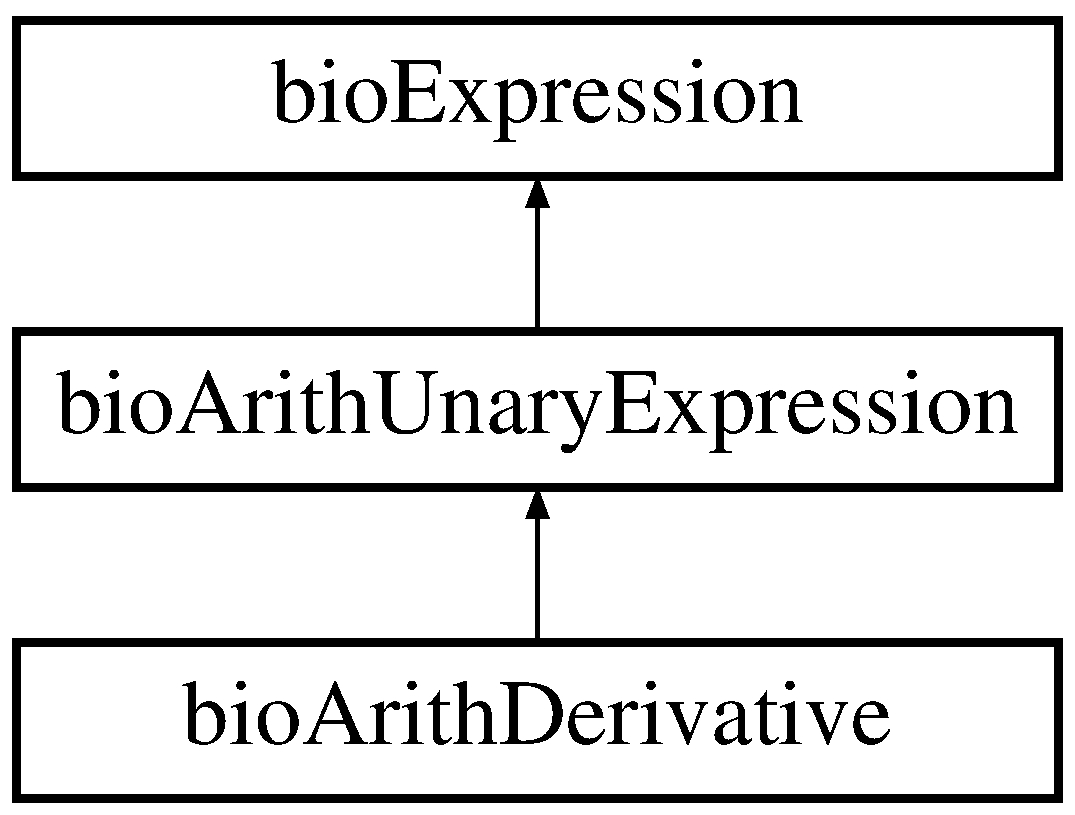
\includegraphics[height=3.000000cm]{classbio_arith_derivative}
\end{center}
\end{figure}
\subsection*{Public Member Functions}
\begin{DoxyCompactItemize}
\item 
\mbox{\Hypertarget{classbio_arith_derivative_a765e22a6898f15287928b1ef0758cca4}\label{classbio_arith_derivative_a765e22a6898f15287928b1ef0758cca4}} 
{\bfseries bio\+Arith\+Derivative} (\hyperlink{classbio_expression_repository}{bio\+Expression\+Repository} $\ast$rep, pat\+U\+Long par, pat\+U\+Long c, pat\+String a\+Literal\+Name, pat\+Error $\ast$\&err)
\item 
virtual pat\+String \hyperlink{classbio_arith_derivative_a5cdf6c4903ec8123b30c0d2ce059718d}{get\+Expression} (pat\+Error $\ast$\&err) const
\item 
virtual pat\+String \hyperlink{classbio_arith_derivative_ac8efdaec7482845045144e134884769a}{get\+Operator\+Name} () const
\item 
virtual pat\+Real \hyperlink{classbio_arith_derivative_a332059cd224467b4a687d39ac705f269}{get\+Value} (pat\+Boolean prepare\+Gradient, pat\+U\+Long current\+Lap, pat\+Error $\ast$\&err)
\item 
virtual \hyperlink{classbio_expression}{bio\+Expression} $\ast$ \hyperlink{classbio_arith_derivative_a6a985cd2c3865e04a3ed54c11a88da17}{get\+Derivative} (pat\+U\+Long a\+Literal\+Id, pat\+Error $\ast$\&err) const
\item 
virtual \hyperlink{classbio_arith_derivative}{bio\+Arith\+Derivative} $\ast$ \hyperlink{classbio_arith_derivative_a9cbc5395703b23816d43580b5482f9f0}{get\+Deep\+Copy} (\hyperlink{classbio_expression_repository}{bio\+Expression\+Repository} $\ast$rep, pat\+Error $\ast$\&err) const
\item 
virtual \hyperlink{classbio_arith_derivative}{bio\+Arith\+Derivative} $\ast$ \hyperlink{classbio_arith_derivative_a37dadf7fcbcfe40bedb900926f3fe974}{get\+Shallow\+Copy} (\hyperlink{classbio_expression_repository}{bio\+Expression\+Repository} $\ast$rep, pat\+Error $\ast$\&err) const
\item 
virtual pat\+Boolean \hyperlink{classbio_arith_derivative_a8de59d734f7c023570046dd184d71a82}{is\+Structurally\+Zero} () const
\item 
virtual pat\+String \hyperlink{classbio_arith_derivative_ae2e8d614fcf2e46d43759c6bab201f30}{get\+Expression\+String} () const
\item 
virtual \hyperlink{classbio_function_and_derivatives}{bio\+Function\+And\+Derivatives} $\ast$ \hyperlink{classbio_arith_derivative_afaa0e62675cc46145231f3e01d38f06a}{get\+Numerical\+Function\+And\+Gradient} (vector$<$ pat\+U\+Long $>$ literal\+Ids, pat\+Boolean compute\+Hessian, pat\+Boolean debug\+Derivatives, pat\+Error $\ast$\&err)
\end{DoxyCompactItemize}
\subsection*{Public Attributes}
\begin{DoxyCompactItemize}
\item 
\mbox{\Hypertarget{classbio_arith_derivative_abb84824917aa60b8294c76b9aa066f64}\label{classbio_arith_derivative_abb84824917aa60b8294c76b9aa066f64}} 
pat\+U\+Long {\bfseries literal\+Id}
\item 
\mbox{\Hypertarget{classbio_arith_derivative_ad4397ec6e219c288783253ac1dd73823}\label{classbio_arith_derivative_ad4397ec6e219c288783253ac1dd73823}} 
pat\+String {\bfseries literal\+Name}
\item 
\mbox{\Hypertarget{classbio_arith_derivative_a8f3bdc79d73d03343d0a96739e6cd8ba}\label{classbio_arith_derivative_a8f3bdc79d73d03343d0a96739e6cd8ba}} 
\hyperlink{classbio_expression}{bio\+Expression} $\ast$ {\bfseries the\+Derivative}
\item 
\mbox{\Hypertarget{classbio_arith_derivative_a3563c317f42fc8b934e96dae0679c4c5}\label{classbio_arith_derivative_a3563c317f42fc8b934e96dae0679c4c5}} 
pat\+U\+Long {\bfseries the\+Derivative\+Id}
\end{DoxyCompactItemize}
\subsection*{Additional Inherited Members}


\subsection{Detailed Description}
Class implementing a node of the tree representing the derivative of the expression with respect to a literal 

\subsection{Member Function Documentation}
\mbox{\Hypertarget{classbio_arith_derivative_a9cbc5395703b23816d43580b5482f9f0}\label{classbio_arith_derivative_a9cbc5395703b23816d43580b5482f9f0}} 
\index{bio\+Arith\+Derivative@{bio\+Arith\+Derivative}!get\+Deep\+Copy@{get\+Deep\+Copy}}
\index{get\+Deep\+Copy@{get\+Deep\+Copy}!bio\+Arith\+Derivative@{bio\+Arith\+Derivative}}
\subsubsection{\texorpdfstring{get\+Deep\+Copy()}{getDeepCopy()}}
{\footnotesize\ttfamily \hyperlink{classbio_arith_derivative}{bio\+Arith\+Derivative} $\ast$ bio\+Arith\+Derivative\+::get\+Deep\+Copy (\begin{DoxyParamCaption}\item[{\hyperlink{classbio_expression_repository}{bio\+Expression\+Repository} $\ast$}]{rep,  }\item[{pat\+Error $\ast$\&}]{err }\end{DoxyParamCaption}) const\hspace{0.3cm}{\ttfamily [virtual]}}

Create a deep copy of the expression and returns a pointer to it. It means that new instances of the children are created. 

Reimplemented from \hyperlink{classbio_expression_a4ee1b8add634078a02eaae26cd40dcc8}{bio\+Expression}.

\mbox{\Hypertarget{classbio_arith_derivative_a6a985cd2c3865e04a3ed54c11a88da17}\label{classbio_arith_derivative_a6a985cd2c3865e04a3ed54c11a88da17}} 
\index{bio\+Arith\+Derivative@{bio\+Arith\+Derivative}!get\+Derivative@{get\+Derivative}}
\index{get\+Derivative@{get\+Derivative}!bio\+Arith\+Derivative@{bio\+Arith\+Derivative}}
\subsubsection{\texorpdfstring{get\+Derivative()}{getDerivative()}}
{\footnotesize\ttfamily \hyperlink{classbio_expression}{bio\+Expression} $\ast$ bio\+Arith\+Derivative\+::get\+Derivative (\begin{DoxyParamCaption}\item[{pat\+U\+Long}]{a\+Literal\+Id,  }\item[{pat\+Error $\ast$\&}]{err }\end{DoxyParamCaption}) const\hspace{0.3cm}{\ttfamily [virtual]}}

\begin{DoxyReturn}{Returns}
value of the derivative w.\+r.\+t literal 
\end{DoxyReturn}

\begin{DoxyParams}{Parameters}
{\em index} & of the literal involved in the derivative \\
\hline
{\em err} & ref. of the pointer to the error object. \\
\hline
\end{DoxyParams}


Reimplemented from \hyperlink{classbio_expression_a5915579d1193f25f216c1e273c97f2ce}{bio\+Expression}.

\mbox{\Hypertarget{classbio_arith_derivative_a5cdf6c4903ec8123b30c0d2ce059718d}\label{classbio_arith_derivative_a5cdf6c4903ec8123b30c0d2ce059718d}} 
\index{bio\+Arith\+Derivative@{bio\+Arith\+Derivative}!get\+Expression@{get\+Expression}}
\index{get\+Expression@{get\+Expression}!bio\+Arith\+Derivative@{bio\+Arith\+Derivative}}
\subsubsection{\texorpdfstring{get\+Expression()}{getExpression()}}
{\footnotesize\ttfamily pat\+String bio\+Arith\+Derivative\+::get\+Expression (\begin{DoxyParamCaption}\item[{pat\+Error $\ast$\&}]{err }\end{DoxyParamCaption}) const\hspace{0.3cm}{\ttfamily [virtual]}}

\begin{DoxyReturn}{Returns}
printed expression 
\end{DoxyReturn}


Reimplemented from \hyperlink{classbio_arith_unary_expression_a974b7779804861f331a75e08db377926}{bio\+Arith\+Unary\+Expression}.

\mbox{\Hypertarget{classbio_arith_derivative_ae2e8d614fcf2e46d43759c6bab201f30}\label{classbio_arith_derivative_ae2e8d614fcf2e46d43759c6bab201f30}} 
\index{bio\+Arith\+Derivative@{bio\+Arith\+Derivative}!get\+Expression\+String@{get\+Expression\+String}}
\index{get\+Expression\+String@{get\+Expression\+String}!bio\+Arith\+Derivative@{bio\+Arith\+Derivative}}
\subsubsection{\texorpdfstring{get\+Expression\+String()}{getExpressionString()}}
{\footnotesize\ttfamily pat\+String bio\+Arith\+Derivative\+::get\+Expression\+String (\begin{DoxyParamCaption}{ }\end{DoxyParamCaption}) const\hspace{0.3cm}{\ttfamily [virtual]}}

Compute a string that represents the expression. It is designed to replace the expression itself when used only for comparison purposes. Code\+: +\{expr1\}\{expr2\}\+: binary plus -\/\{expr1\}\{expr2\}\+: binary minus \{expr1\}\{expr2\}\+: multiplication /\{expr1\}\{expr2\}\+: division $^\wedge$\{expr1\}\{expr2\}\+: power \&\{expr1\}\{expr2\}\+: and $\vert$\{expr1\}\{expr2\}\+: or =\{expr1\}\{expr2\}\+: equal !=\{expr1\}\{expr2\}\+: not equal $<$\{expr1\}\{expr2\}\+: lesser than $<$=\{expr1\}\{expr2\}\+: lesser or equal to $>$\{expr1\}\{expr2\}\+: greater than $>$=\{expr1\}\{expr2\}\+: greater or equal to \$A\{expr\}\+: abs \$D\mbox{[}expr\mbox{]}\mbox{[}\{expr1\}...\{exprN\}\mbox{]}\+: dictionary (\hyperlink{classbio_arith_elem}{bio\+Arith\+Elem}) \$E\{expr\}\+: exp \$L\{expr\}\+: log \$M\{expr\}\+: Unary minus \$\+Piterator\+\_\+name\{expr\}\+: prod \$Q\{string1\}\{string2\}\+: sequence \$\+Siterator\+\_\+name\{expr\}\+: sum \$\+Ziterator\+\_\+name\mbox{[}\{expr1\}...\{exprN\}\mbox{]}\+: merged sum \{expr1\}\{expr2\}...\{exprN\}//\+: list of expressions number\+: constant \#id\+: literal \&id\+: random 

Reimplemented from \hyperlink{classbio_expression_a3e4b4dca58dbbc6f0e411b30eb3f60b4}{bio\+Expression}.

\mbox{\Hypertarget{classbio_arith_derivative_afaa0e62675cc46145231f3e01d38f06a}\label{classbio_arith_derivative_afaa0e62675cc46145231f3e01d38f06a}} 
\index{bio\+Arith\+Derivative@{bio\+Arith\+Derivative}!get\+Numerical\+Function\+And\+Gradient@{get\+Numerical\+Function\+And\+Gradient}}
\index{get\+Numerical\+Function\+And\+Gradient@{get\+Numerical\+Function\+And\+Gradient}!bio\+Arith\+Derivative@{bio\+Arith\+Derivative}}
\subsubsection{\texorpdfstring{get\+Numerical\+Function\+And\+Gradient()}{getNumericalFunctionAndGradient()}}
{\footnotesize\ttfamily \hyperlink{classbio_function_and_derivatives}{bio\+Function\+And\+Derivatives} $\ast$ bio\+Arith\+Derivative\+::get\+Numerical\+Function\+And\+Gradient (\begin{DoxyParamCaption}\item[{vector$<$ pat\+U\+Long $>$}]{literal\+Ids,  }\item[{pat\+Boolean}]{compute\+Hessian,  }\item[{pat\+Boolean}]{debug\+Derivatives,  }\item[{pat\+Error $\ast$\&}]{err }\end{DoxyParamCaption})\hspace{0.3cm}{\ttfamily [virtual]}}

\begin{DoxyReturn}{Returns}
value and gradient of the expression 
\end{DoxyReturn}

\begin{DoxyParams}{Parameters}
{\em err} & ref. of the pointer to the error object. \\
\hline
\end{DoxyParams}


Reimplemented from \hyperlink{classbio_expression_a91c81ce80c9e972c913b10f5f3c1ed13}{bio\+Expression}.

\mbox{\Hypertarget{classbio_arith_derivative_ac8efdaec7482845045144e134884769a}\label{classbio_arith_derivative_ac8efdaec7482845045144e134884769a}} 
\index{bio\+Arith\+Derivative@{bio\+Arith\+Derivative}!get\+Operator\+Name@{get\+Operator\+Name}}
\index{get\+Operator\+Name@{get\+Operator\+Name}!bio\+Arith\+Derivative@{bio\+Arith\+Derivative}}
\subsubsection{\texorpdfstring{get\+Operator\+Name()}{getOperatorName()}}
{\footnotesize\ttfamily pat\+String bio\+Arith\+Derivative\+::get\+Operator\+Name (\begin{DoxyParamCaption}{ }\end{DoxyParamCaption}) const\hspace{0.3cm}{\ttfamily [virtual]}}

\begin{DoxyReturn}{Returns}
name of the operator 
\end{DoxyReturn}


Reimplemented from \hyperlink{classbio_expression_a2353a4afb3a2b0af7c63aba086a72bde}{bio\+Expression}.

\mbox{\Hypertarget{classbio_arith_derivative_a37dadf7fcbcfe40bedb900926f3fe974}\label{classbio_arith_derivative_a37dadf7fcbcfe40bedb900926f3fe974}} 
\index{bio\+Arith\+Derivative@{bio\+Arith\+Derivative}!get\+Shallow\+Copy@{get\+Shallow\+Copy}}
\index{get\+Shallow\+Copy@{get\+Shallow\+Copy}!bio\+Arith\+Derivative@{bio\+Arith\+Derivative}}
\subsubsection{\texorpdfstring{get\+Shallow\+Copy()}{getShallowCopy()}}
{\footnotesize\ttfamily \hyperlink{classbio_arith_derivative}{bio\+Arith\+Derivative} $\ast$ bio\+Arith\+Derivative\+::get\+Shallow\+Copy (\begin{DoxyParamCaption}\item[{\hyperlink{classbio_expression_repository}{bio\+Expression\+Repository} $\ast$}]{rep,  }\item[{pat\+Error $\ast$\&}]{err }\end{DoxyParamCaption}) const\hspace{0.3cm}{\ttfamily [virtual]}}

Create a shallow copy of the expression and returns a pointer to it. It means that no new instance of the children are created. It is typically called by the repository 

Reimplemented from \hyperlink{classbio_expression_a442534762693b92baaf33928979a1bf8}{bio\+Expression}.

\mbox{\Hypertarget{classbio_arith_derivative_a332059cd224467b4a687d39ac705f269}\label{classbio_arith_derivative_a332059cd224467b4a687d39ac705f269}} 
\index{bio\+Arith\+Derivative@{bio\+Arith\+Derivative}!get\+Value@{get\+Value}}
\index{get\+Value@{get\+Value}!bio\+Arith\+Derivative@{bio\+Arith\+Derivative}}
\subsubsection{\texorpdfstring{get\+Value()}{getValue()}}
{\footnotesize\ttfamily pat\+Real bio\+Arith\+Derivative\+::get\+Value (\begin{DoxyParamCaption}\item[{pat\+Boolean}]{prepare\+Gradient,  }\item[{pat\+U\+Long}]{current\+Lap,  }\item[{pat\+Error $\ast$\&}]{err }\end{DoxyParamCaption})\hspace{0.3cm}{\ttfamily [virtual]}}

\begin{DoxyReturn}{Returns}
value of the expression 
\end{DoxyReturn}

\begin{DoxyParams}{Parameters}
{\em err} & ref. of the pointer to the error object. \\
\hline
\end{DoxyParams}


Reimplemented from \hyperlink{classbio_expression_af58662a5d4d456f15bc4f2c9bd4f8a5b}{bio\+Expression}.

\mbox{\Hypertarget{classbio_arith_derivative_a8de59d734f7c023570046dd184d71a82}\label{classbio_arith_derivative_a8de59d734f7c023570046dd184d71a82}} 
\index{bio\+Arith\+Derivative@{bio\+Arith\+Derivative}!is\+Structurally\+Zero@{is\+Structurally\+Zero}}
\index{is\+Structurally\+Zero@{is\+Structurally\+Zero}!bio\+Arith\+Derivative@{bio\+Arith\+Derivative}}
\subsubsection{\texorpdfstring{is\+Structurally\+Zero()}{isStructurallyZero()}}
{\footnotesize\ttfamily pat\+Boolean bio\+Arith\+Derivative\+::is\+Structurally\+Zero (\begin{DoxyParamCaption}{ }\end{DoxyParamCaption}) const\hspace{0.3cm}{\ttfamily [virtual]}}

return pat\+T\+R\+UE if the expression is structurally 0 so that there is no need to evaluate it. In the base class, it return pat\+F\+A\+L\+SE. 

Reimplemented from \hyperlink{classbio_expression_a264c6d78671610ada8261d698e4c4c42}{bio\+Expression}.



The documentation for this class was generated from the following files\+:\begin{DoxyCompactItemize}
\item 
bio\+Arith\+Derivative.\+h\item 
bio\+Arith\+Derivative.\+cc\end{DoxyCompactItemize}

\hypertarget{classbio_arith_divide}{}\section{bio\+Arith\+Divide Class Reference}
\label{classbio_arith_divide}\index{bio\+Arith\+Divide@{bio\+Arith\+Divide}}


{\ttfamily \#include $<$bio\+Arith\+Divide.\+h$>$}

Inheritance diagram for bio\+Arith\+Divide\+:\begin{figure}[H]
\begin{center}
\leavevmode
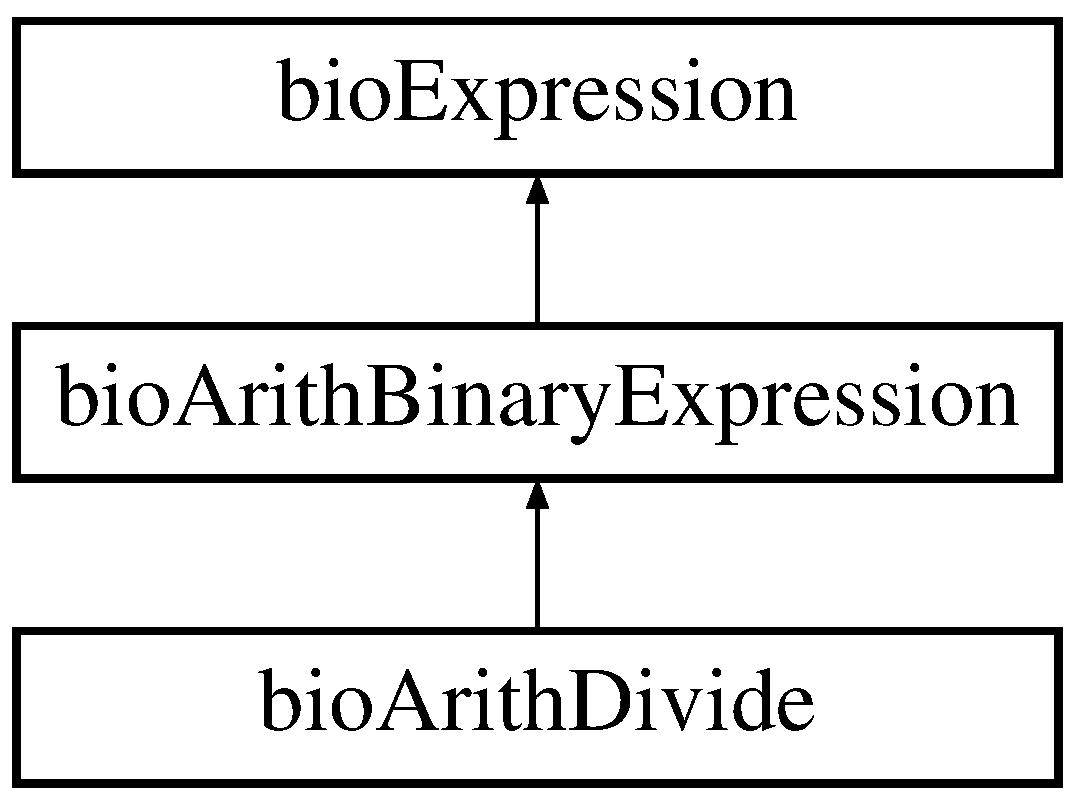
\includegraphics[height=3.000000cm]{classbio_arith_divide}
\end{center}
\end{figure}
\subsection*{Public Member Functions}
\begin{DoxyCompactItemize}
\item 
\mbox{\Hypertarget{classbio_arith_divide_a5aeb2aa48813d8c1a47d27dc02f4bf34}\label{classbio_arith_divide_a5aeb2aa48813d8c1a47d27dc02f4bf34}} 
{\bfseries bio\+Arith\+Divide} (\hyperlink{classbio_expression_repository}{bio\+Expression\+Repository} $\ast$rep, pat\+U\+Long par, pat\+U\+Long left, pat\+U\+Long right, pat\+Error $\ast$\&err)
\item 
virtual pat\+String \hyperlink{classbio_arith_divide_a544e0dc66cfb2be23226a968b5d7c5cb}{get\+Operator\+Name} () const
\item 
virtual pat\+Real \hyperlink{classbio_arith_divide_a8c979df7aee15572084ac982d1bd0740}{get\+Value} (pat\+Boolean prepare\+Gradient, pat\+U\+Long current\+Lap, pat\+Error $\ast$\&err)
\item 
virtual \hyperlink{classbio_expression}{bio\+Expression} $\ast$ \hyperlink{classbio_arith_divide_a9a30c3d5586f0bce3b09cc2c932e5f67}{get\+Derivative} (pat\+U\+Long a\+Literal\+Id, pat\+Error $\ast$\&err) const
\item 
virtual \hyperlink{classbio_arith_divide}{bio\+Arith\+Divide} $\ast$ \hyperlink{classbio_arith_divide_aa867fd8e74e654f419eee829a08e816c}{get\+Deep\+Copy} (\hyperlink{classbio_expression_repository}{bio\+Expression\+Repository} $\ast$rep, pat\+Error $\ast$\&err) const
\item 
virtual \hyperlink{classbio_arith_divide}{bio\+Arith\+Divide} $\ast$ \hyperlink{classbio_arith_divide_a381a838c2c02b9f1cf9c7a4b6586dbca}{get\+Shallow\+Copy} (\hyperlink{classbio_expression_repository}{bio\+Expression\+Repository} $\ast$rep, pat\+Error $\ast$\&err) const
\item 
virtual pat\+Boolean \hyperlink{classbio_arith_divide_a0363fd1159b9167508dcf989844eebb7}{is\+Structurally\+Zero} () const
\item 
virtual pat\+String \hyperlink{classbio_arith_divide_a11ecaa69e3d86cb8598770f40ec03753}{get\+Expression\+String} () const
\item 
virtual \hyperlink{classbio_function_and_derivatives}{bio\+Function\+And\+Derivatives} $\ast$ \hyperlink{classbio_arith_divide_a29465844ff4722a8d542c8a6935c2686}{get\+Numerical\+Function\+And\+Gradient} (vector$<$ pat\+U\+Long $>$ literal\+Ids, pat\+Boolean compute\+Hessian, pat\+Boolean debug\+Derivatives, pat\+Error $\ast$\&err)
\end{DoxyCompactItemize}
\subsection*{Additional Inherited Members}


\subsection{Detailed Description}
Class implementing a node for a division operation 

\subsection{Member Function Documentation}
\mbox{\Hypertarget{classbio_arith_divide_aa867fd8e74e654f419eee829a08e816c}\label{classbio_arith_divide_aa867fd8e74e654f419eee829a08e816c}} 
\index{bio\+Arith\+Divide@{bio\+Arith\+Divide}!get\+Deep\+Copy@{get\+Deep\+Copy}}
\index{get\+Deep\+Copy@{get\+Deep\+Copy}!bio\+Arith\+Divide@{bio\+Arith\+Divide}}
\subsubsection{\texorpdfstring{get\+Deep\+Copy()}{getDeepCopy()}}
{\footnotesize\ttfamily \hyperlink{classbio_arith_divide}{bio\+Arith\+Divide} $\ast$ bio\+Arith\+Divide\+::get\+Deep\+Copy (\begin{DoxyParamCaption}\item[{\hyperlink{classbio_expression_repository}{bio\+Expression\+Repository} $\ast$}]{rep,  }\item[{pat\+Error $\ast$\&}]{err }\end{DoxyParamCaption}) const\hspace{0.3cm}{\ttfamily [virtual]}}

Create a deep copy of the expression and returns a pointer to it. It means that new instances of the children are created. 

Reimplemented from \hyperlink{classbio_expression_a4ee1b8add634078a02eaae26cd40dcc8}{bio\+Expression}.

\mbox{\Hypertarget{classbio_arith_divide_a9a30c3d5586f0bce3b09cc2c932e5f67}\label{classbio_arith_divide_a9a30c3d5586f0bce3b09cc2c932e5f67}} 
\index{bio\+Arith\+Divide@{bio\+Arith\+Divide}!get\+Derivative@{get\+Derivative}}
\index{get\+Derivative@{get\+Derivative}!bio\+Arith\+Divide@{bio\+Arith\+Divide}}
\subsubsection{\texorpdfstring{get\+Derivative()}{getDerivative()}}
{\footnotesize\ttfamily \hyperlink{classbio_expression}{bio\+Expression} $\ast$ bio\+Arith\+Divide\+::get\+Derivative (\begin{DoxyParamCaption}\item[{pat\+U\+Long}]{a\+Literal\+Id,  }\item[{pat\+Error $\ast$\&}]{err }\end{DoxyParamCaption}) const\hspace{0.3cm}{\ttfamily [virtual]}}

\begin{DoxyReturn}{Returns}
value of the derivative w.\+r.\+t literal 
\end{DoxyReturn}

\begin{DoxyParams}{Parameters}
{\em index} & of the literal involved in the derivative \\
\hline
{\em err} & ref. of the pointer to the error object. \\
\hline
\end{DoxyParams}


Reimplemented from \hyperlink{classbio_expression_a5915579d1193f25f216c1e273c97f2ce}{bio\+Expression}.

\mbox{\Hypertarget{classbio_arith_divide_a11ecaa69e3d86cb8598770f40ec03753}\label{classbio_arith_divide_a11ecaa69e3d86cb8598770f40ec03753}} 
\index{bio\+Arith\+Divide@{bio\+Arith\+Divide}!get\+Expression\+String@{get\+Expression\+String}}
\index{get\+Expression\+String@{get\+Expression\+String}!bio\+Arith\+Divide@{bio\+Arith\+Divide}}
\subsubsection{\texorpdfstring{get\+Expression\+String()}{getExpressionString()}}
{\footnotesize\ttfamily pat\+String bio\+Arith\+Divide\+::get\+Expression\+String (\begin{DoxyParamCaption}{ }\end{DoxyParamCaption}) const\hspace{0.3cm}{\ttfamily [virtual]}}

Compute a string that represents the expression. It is designed to replace the expression itself when used only for comparison purposes. Code\+: +\{expr1\}\{expr2\}\+: binary plus -\/\{expr1\}\{expr2\}\+: binary minus \{expr1\}\{expr2\}\+: multiplication /\{expr1\}\{expr2\}\+: division $^\wedge$\{expr1\}\{expr2\}\+: power \&\{expr1\}\{expr2\}\+: and $\vert$\{expr1\}\{expr2\}\+: or =\{expr1\}\{expr2\}\+: equal !=\{expr1\}\{expr2\}\+: not equal $<$\{expr1\}\{expr2\}\+: lesser than $<$=\{expr1\}\{expr2\}\+: lesser or equal to $>$\{expr1\}\{expr2\}\+: greater than $>$=\{expr1\}\{expr2\}\+: greater or equal to \$A\{expr\}\+: abs \$D\mbox{[}expr\mbox{]}\mbox{[}\{expr1\}...\{exprN\}\mbox{]}\+: dictionary (\hyperlink{classbio_arith_elem}{bio\+Arith\+Elem}) \$E\{expr\}\+: exp \$L\{expr\}\+: log \$M\{expr\}\+: Unary minus \$\+Piterator\+\_\+name\{expr\}\+: prod \$Q\{string1\}\{string2\}\+: sequence \$\+Siterator\+\_\+name\{expr\}\+: sum \$\+Ziterator\+\_\+name\mbox{[}\{expr1\}...\{exprN\}\mbox{]}\+: merged sum \{expr1\}\{expr2\}...\{exprN\}//\+: list of expressions number\+: constant \#id\+: literal \&id\+: random 

Reimplemented from \hyperlink{classbio_expression_a3e4b4dca58dbbc6f0e411b30eb3f60b4}{bio\+Expression}.

\mbox{\Hypertarget{classbio_arith_divide_a29465844ff4722a8d542c8a6935c2686}\label{classbio_arith_divide_a29465844ff4722a8d542c8a6935c2686}} 
\index{bio\+Arith\+Divide@{bio\+Arith\+Divide}!get\+Numerical\+Function\+And\+Gradient@{get\+Numerical\+Function\+And\+Gradient}}
\index{get\+Numerical\+Function\+And\+Gradient@{get\+Numerical\+Function\+And\+Gradient}!bio\+Arith\+Divide@{bio\+Arith\+Divide}}
\subsubsection{\texorpdfstring{get\+Numerical\+Function\+And\+Gradient()}{getNumericalFunctionAndGradient()}}
{\footnotesize\ttfamily \hyperlink{classbio_function_and_derivatives}{bio\+Function\+And\+Derivatives} $\ast$ bio\+Arith\+Divide\+::get\+Numerical\+Function\+And\+Gradient (\begin{DoxyParamCaption}\item[{vector$<$ pat\+U\+Long $>$}]{literal\+Ids,  }\item[{pat\+Boolean}]{compute\+Hessian,  }\item[{pat\+Boolean}]{debug\+Derivatives,  }\item[{pat\+Error $\ast$\&}]{err }\end{DoxyParamCaption})\hspace{0.3cm}{\ttfamily [virtual]}}

\begin{DoxyReturn}{Returns}
value and gradient of the expression 
\end{DoxyReturn}

\begin{DoxyParams}{Parameters}
{\em err} & ref. of the pointer to the error object. \\
\hline
\end{DoxyParams}


Reimplemented from \hyperlink{classbio_expression_a91c81ce80c9e972c913b10f5f3c1ed13}{bio\+Expression}.

\mbox{\Hypertarget{classbio_arith_divide_a544e0dc66cfb2be23226a968b5d7c5cb}\label{classbio_arith_divide_a544e0dc66cfb2be23226a968b5d7c5cb}} 
\index{bio\+Arith\+Divide@{bio\+Arith\+Divide}!get\+Operator\+Name@{get\+Operator\+Name}}
\index{get\+Operator\+Name@{get\+Operator\+Name}!bio\+Arith\+Divide@{bio\+Arith\+Divide}}
\subsubsection{\texorpdfstring{get\+Operator\+Name()}{getOperatorName()}}
{\footnotesize\ttfamily pat\+String bio\+Arith\+Divide\+::get\+Operator\+Name (\begin{DoxyParamCaption}{ }\end{DoxyParamCaption}) const\hspace{0.3cm}{\ttfamily [virtual]}}

\begin{DoxyReturn}{Returns}
name of the operator 
\end{DoxyReturn}


Reimplemented from \hyperlink{classbio_expression_a2353a4afb3a2b0af7c63aba086a72bde}{bio\+Expression}.

\mbox{\Hypertarget{classbio_arith_divide_a381a838c2c02b9f1cf9c7a4b6586dbca}\label{classbio_arith_divide_a381a838c2c02b9f1cf9c7a4b6586dbca}} 
\index{bio\+Arith\+Divide@{bio\+Arith\+Divide}!get\+Shallow\+Copy@{get\+Shallow\+Copy}}
\index{get\+Shallow\+Copy@{get\+Shallow\+Copy}!bio\+Arith\+Divide@{bio\+Arith\+Divide}}
\subsubsection{\texorpdfstring{get\+Shallow\+Copy()}{getShallowCopy()}}
{\footnotesize\ttfamily \hyperlink{classbio_arith_divide}{bio\+Arith\+Divide} $\ast$ bio\+Arith\+Divide\+::get\+Shallow\+Copy (\begin{DoxyParamCaption}\item[{\hyperlink{classbio_expression_repository}{bio\+Expression\+Repository} $\ast$}]{rep,  }\item[{pat\+Error $\ast$\&}]{err }\end{DoxyParamCaption}) const\hspace{0.3cm}{\ttfamily [virtual]}}

Create a shallow copy of the expression and returns a pointer to it. It means that no new instance of the children are created. It is typically called by the repository 

Reimplemented from \hyperlink{classbio_expression_a442534762693b92baaf33928979a1bf8}{bio\+Expression}.

\mbox{\Hypertarget{classbio_arith_divide_a8c979df7aee15572084ac982d1bd0740}\label{classbio_arith_divide_a8c979df7aee15572084ac982d1bd0740}} 
\index{bio\+Arith\+Divide@{bio\+Arith\+Divide}!get\+Value@{get\+Value}}
\index{get\+Value@{get\+Value}!bio\+Arith\+Divide@{bio\+Arith\+Divide}}
\subsubsection{\texorpdfstring{get\+Value()}{getValue()}}
{\footnotesize\ttfamily pat\+Real bio\+Arith\+Divide\+::get\+Value (\begin{DoxyParamCaption}\item[{pat\+Boolean}]{prepare\+Gradient,  }\item[{pat\+U\+Long}]{current\+Lap,  }\item[{pat\+Error $\ast$\&}]{err }\end{DoxyParamCaption})\hspace{0.3cm}{\ttfamily [virtual]}}

\begin{DoxyReturn}{Returns}
value of the expression 
\end{DoxyReturn}

\begin{DoxyParams}{Parameters}
{\em err} & ref. of the pointer to the error object. \\
\hline
\end{DoxyParams}


Reimplemented from \hyperlink{classbio_expression_af58662a5d4d456f15bc4f2c9bd4f8a5b}{bio\+Expression}.

\mbox{\Hypertarget{classbio_arith_divide_a0363fd1159b9167508dcf989844eebb7}\label{classbio_arith_divide_a0363fd1159b9167508dcf989844eebb7}} 
\index{bio\+Arith\+Divide@{bio\+Arith\+Divide}!is\+Structurally\+Zero@{is\+Structurally\+Zero}}
\index{is\+Structurally\+Zero@{is\+Structurally\+Zero}!bio\+Arith\+Divide@{bio\+Arith\+Divide}}
\subsubsection{\texorpdfstring{is\+Structurally\+Zero()}{isStructurallyZero()}}
{\footnotesize\ttfamily pat\+Boolean bio\+Arith\+Divide\+::is\+Structurally\+Zero (\begin{DoxyParamCaption}{ }\end{DoxyParamCaption}) const\hspace{0.3cm}{\ttfamily [virtual]}}

return pat\+T\+R\+UE if the expression is structurally 0 so that there is no need to evaluate it. In the base class, it return pat\+F\+A\+L\+SE. 

Reimplemented from \hyperlink{classbio_expression_a264c6d78671610ada8261d698e4c4c42}{bio\+Expression}.



The documentation for this class was generated from the following files\+:\begin{DoxyCompactItemize}
\item 
bio\+Arith\+Divide.\+h\item 
bio\+Arith\+Divide.\+cc\end{DoxyCompactItemize}

\hypertarget{classbio_arith_elem}{}\section{bio\+Arith\+Elem Class Reference}
\label{classbio_arith_elem}\index{bio\+Arith\+Elem@{bio\+Arith\+Elem}}


{\ttfamily \#include $<$bio\+Arith\+Elem.\+h$>$}

Inheritance diagram for bio\+Arith\+Elem\+:\begin{figure}[H]
\begin{center}
\leavevmode
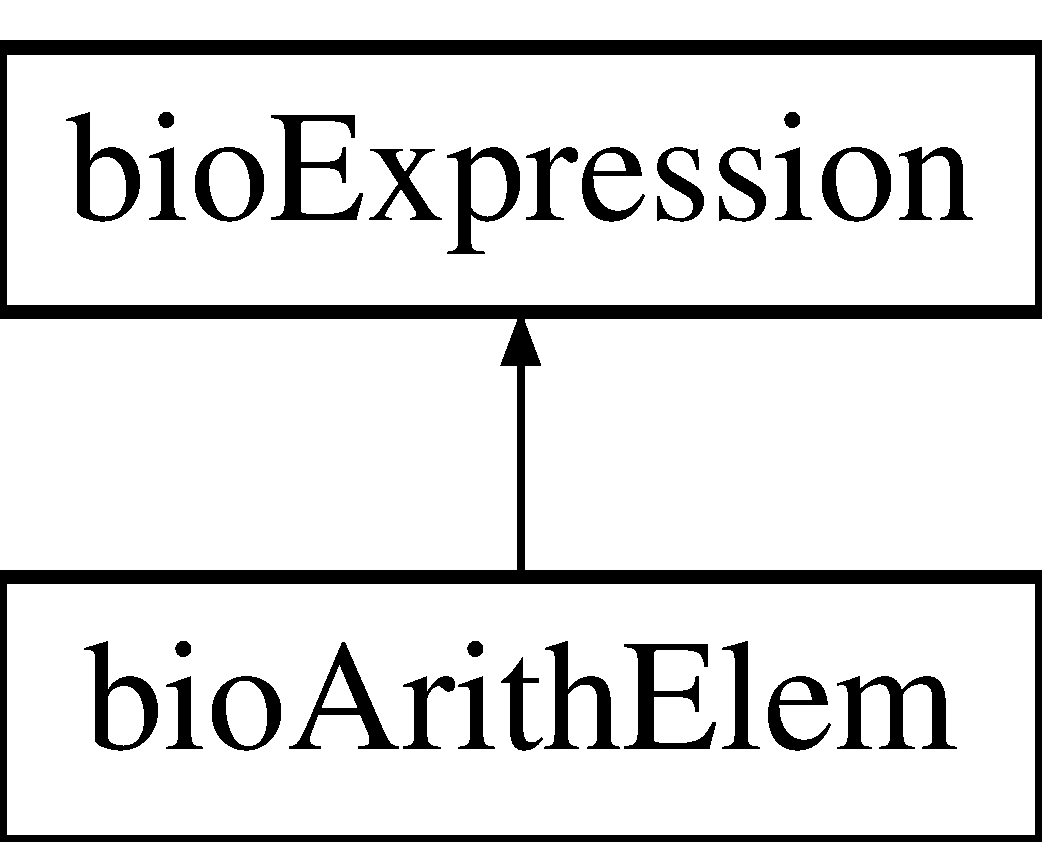
\includegraphics[height=2.000000cm]{classbio_arith_elem}
\end{center}
\end{figure}
\subsection*{Public Member Functions}
\begin{DoxyCompactItemize}
\item 
\mbox{\Hypertarget{classbio_arith_elem_ae74bb8f951dc8a93bd5b957df741a968}\label{classbio_arith_elem_ae74bb8f951dc8a93bd5b957df741a968}} 
{\bfseries bio\+Arith\+Elem} (\hyperlink{classbio_expression_repository}{bio\+Expression\+Repository} $\ast$rep, pat\+U\+Long par, pat\+U\+Long ind, map$<$ pat\+U\+Long, pat\+U\+Long $>$ a\+Dict, pat\+U\+Long def, pat\+Error $\ast$\&err)
\item 
virtual pat\+Boolean \hyperlink{classbio_arith_elem_a9d64d5197cb2cab10396c3e9d8add42b}{is\+Structurally\+Zero} () const
\item 
virtual pat\+String \hyperlink{classbio_arith_elem_a501dc3818a694f54765ad69a4a67279e}{get\+Operator\+Name} () const
\item 
virtual pat\+Real \hyperlink{classbio_arith_elem_aac719574ab496e1b3341b9e4b71a7986}{get\+Value} (pat\+Boolean prepare\+Gradient, pat\+U\+Long current\+Lap, pat\+Error $\ast$\&err)
\item 
virtual \hyperlink{classbio_expression}{bio\+Expression} $\ast$ \hyperlink{classbio_arith_elem_a0905b898fe28bad14df85cd2bbcf1e1c}{get\+Derivative} (pat\+U\+Long a\+Literal\+Id, pat\+Error $\ast$\&err) const
\item 
virtual \hyperlink{classbio_arith_elem}{bio\+Arith\+Elem} $\ast$ \hyperlink{classbio_arith_elem_a3635350e02e428a9fe9dfeaac6247514}{get\+Deep\+Copy} (\hyperlink{classbio_expression_repository}{bio\+Expression\+Repository} $\ast$rep, pat\+Error $\ast$\&err) const
\item 
virtual \hyperlink{classbio_arith_elem}{bio\+Arith\+Elem} $\ast$ \hyperlink{classbio_arith_elem_a481ee9025662995608714643a1239a26}{get\+Shallow\+Copy} (\hyperlink{classbio_expression_repository}{bio\+Expression\+Repository} $\ast$rep, pat\+Error $\ast$\&err) const
\item 
virtual pat\+String \hyperlink{classbio_arith_elem_a729f5a91619948fa58f7b4902741a2f4}{get\+Expression} (pat\+Error $\ast$\&err) const
\item 
\mbox{\Hypertarget{classbio_arith_elem_aabc496888ad863c815d95dc1a7bbd2a3}\label{classbio_arith_elem_aabc496888ad863c815d95dc1a7bbd2a3}} 
virtual pat\+Boolean {\bfseries depends\+Of} (pat\+U\+Long a\+Literal\+Id) const
\item 
\mbox{\Hypertarget{classbio_arith_elem_aeb9f6d20f9802f29b22d94ca442f3015}\label{classbio_arith_elem_aeb9f6d20f9802f29b22d94ca442f3015}} 
virtual void {\bfseries simplify\+Zeros} (pat\+Error $\ast$\&err)
\item 
\mbox{\Hypertarget{classbio_arith_elem_af8eac0387ed4c5eaec6fdf0e48498770}\label{classbio_arith_elem_af8eac0387ed4c5eaec6fdf0e48498770}} 
virtual pat\+U\+Long {\bfseries get\+Number\+Of\+Operations} () const
\item 
\mbox{\Hypertarget{classbio_arith_elem_ab401b4ac4812ad95cda9d98b39fc1a8d}\label{classbio_arith_elem_ab401b4ac4812ad95cda9d98b39fc1a8d}} 
pat\+U\+Long {\bfseries last\+Index} () const
\item 
virtual pat\+String \hyperlink{classbio_arith_elem_a0ea23c1cc50f06dec01ba195392c8417}{get\+Expression\+String} () const
\item 
\mbox{\Hypertarget{classbio_arith_elem_a6080c51944897aae209c109fbde81d6a}\label{classbio_arith_elem_a6080c51944897aae209c109fbde81d6a}} 
pat\+Boolean {\bfseries contains\+An\+Integral} () const
\item 
\mbox{\Hypertarget{classbio_arith_elem_aa32c8faf83cdfb59f1d981046a0b5085}\label{classbio_arith_elem_aa32c8faf83cdfb59f1d981046a0b5085}} 
pat\+Boolean {\bfseries contains\+An\+Iterator} () const
\item 
\mbox{\Hypertarget{classbio_arith_elem_acc7b5c4774f9b131053717d1cb94654d}\label{classbio_arith_elem_acc7b5c4774f9b131053717d1cb94654d}} 
pat\+Boolean {\bfseries contains\+An\+Iterator\+On\+Rows} () const
\item 
\mbox{\Hypertarget{classbio_arith_elem_a0a3c0dd7f8d36f527b8da73390bd39b7}\label{classbio_arith_elem_a0a3c0dd7f8d36f527b8da73390bd39b7}} 
pat\+Boolean {\bfseries contains\+A\+Sequence} () const
\item 
\mbox{\Hypertarget{classbio_arith_elem_a29c15adab07861e48a20562cf57c38dc}\label{classbio_arith_elem_a29c15adab07861e48a20562cf57c38dc}} 
virtual void {\bfseries collect\+Expression\+Ids} (set$<$ pat\+U\+Long $>$ $\ast$s) const
\item 
virtual \hyperlink{classbio_function_and_derivatives}{bio\+Function\+And\+Derivatives} $\ast$ \hyperlink{classbio_arith_elem_a3aa76152765b0c8acb778f2070ded9f8}{get\+Numerical\+Function\+And\+Gradient} (vector$<$ pat\+U\+Long $>$ literal\+Ids, pat\+Boolean compute\+Hessian, pat\+Boolean debug\+Derivatives, pat\+Error $\ast$\&err)
\item 
\mbox{\Hypertarget{classbio_arith_elem_ac6e02bb52b650db18e6ab66e36b2b557}\label{classbio_arith_elem_ac6e02bb52b650db18e6ab66e36b2b557}} 
virtual pat\+String {\bfseries check} (pat\+Error $\ast$\&err) const
\end{DoxyCompactItemize}
\subsection*{Additional Inherited Members}


\subsection{Detailed Description}
We have a dictionary of expressions, mapping values to expressions. The value itself is first computed, and the associated expression is then evaluated. 

\subsection{Member Function Documentation}
\mbox{\Hypertarget{classbio_arith_elem_a3635350e02e428a9fe9dfeaac6247514}\label{classbio_arith_elem_a3635350e02e428a9fe9dfeaac6247514}} 
\index{bio\+Arith\+Elem@{bio\+Arith\+Elem}!get\+Deep\+Copy@{get\+Deep\+Copy}}
\index{get\+Deep\+Copy@{get\+Deep\+Copy}!bio\+Arith\+Elem@{bio\+Arith\+Elem}}
\subsubsection{\texorpdfstring{get\+Deep\+Copy()}{getDeepCopy()}}
{\footnotesize\ttfamily \hyperlink{classbio_arith_elem}{bio\+Arith\+Elem} $\ast$ bio\+Arith\+Elem\+::get\+Deep\+Copy (\begin{DoxyParamCaption}\item[{\hyperlink{classbio_expression_repository}{bio\+Expression\+Repository} $\ast$}]{rep,  }\item[{pat\+Error $\ast$\&}]{err }\end{DoxyParamCaption}) const\hspace{0.3cm}{\ttfamily [virtual]}}

Create a deep copy of the expression and returns a pointer to it. It means that new instances of the children are created. 

Reimplemented from \hyperlink{classbio_expression_a4ee1b8add634078a02eaae26cd40dcc8}{bio\+Expression}.

\mbox{\Hypertarget{classbio_arith_elem_a0905b898fe28bad14df85cd2bbcf1e1c}\label{classbio_arith_elem_a0905b898fe28bad14df85cd2bbcf1e1c}} 
\index{bio\+Arith\+Elem@{bio\+Arith\+Elem}!get\+Derivative@{get\+Derivative}}
\index{get\+Derivative@{get\+Derivative}!bio\+Arith\+Elem@{bio\+Arith\+Elem}}
\subsubsection{\texorpdfstring{get\+Derivative()}{getDerivative()}}
{\footnotesize\ttfamily \hyperlink{classbio_expression}{bio\+Expression} $\ast$ bio\+Arith\+Elem\+::get\+Derivative (\begin{DoxyParamCaption}\item[{pat\+U\+Long}]{a\+Literal\+Id,  }\item[{pat\+Error $\ast$\&}]{err }\end{DoxyParamCaption}) const\hspace{0.3cm}{\ttfamily [virtual]}}

\begin{DoxyReturn}{Returns}
value of the derivative w.\+r.\+t literal 
\end{DoxyReturn}

\begin{DoxyParams}{Parameters}
{\em index} & of the literal involved in the derivative \\
\hline
{\em err} & ref. of the pointer to the error object. \\
\hline
\end{DoxyParams}


Reimplemented from \hyperlink{classbio_expression_a5915579d1193f25f216c1e273c97f2ce}{bio\+Expression}.

\mbox{\Hypertarget{classbio_arith_elem_a729f5a91619948fa58f7b4902741a2f4}\label{classbio_arith_elem_a729f5a91619948fa58f7b4902741a2f4}} 
\index{bio\+Arith\+Elem@{bio\+Arith\+Elem}!get\+Expression@{get\+Expression}}
\index{get\+Expression@{get\+Expression}!bio\+Arith\+Elem@{bio\+Arith\+Elem}}
\subsubsection{\texorpdfstring{get\+Expression()}{getExpression()}}
{\footnotesize\ttfamily pat\+String bio\+Arith\+Elem\+::get\+Expression (\begin{DoxyParamCaption}\item[{pat\+Error $\ast$\&}]{err }\end{DoxyParamCaption}) const\hspace{0.3cm}{\ttfamily [virtual]}}

\begin{DoxyReturn}{Returns}
printed expression 
\end{DoxyReturn}


Reimplemented from \hyperlink{classbio_expression_a66a83eb0caac18dd5e568ffde5a8b5d4}{bio\+Expression}.

\mbox{\Hypertarget{classbio_arith_elem_a0ea23c1cc50f06dec01ba195392c8417}\label{classbio_arith_elem_a0ea23c1cc50f06dec01ba195392c8417}} 
\index{bio\+Arith\+Elem@{bio\+Arith\+Elem}!get\+Expression\+String@{get\+Expression\+String}}
\index{get\+Expression\+String@{get\+Expression\+String}!bio\+Arith\+Elem@{bio\+Arith\+Elem}}
\subsubsection{\texorpdfstring{get\+Expression\+String()}{getExpressionString()}}
{\footnotesize\ttfamily pat\+String bio\+Arith\+Elem\+::get\+Expression\+String (\begin{DoxyParamCaption}{ }\end{DoxyParamCaption}) const\hspace{0.3cm}{\ttfamily [virtual]}}

Compute a string that represents the expression. It is designed to replace the expression itself when used only for comparison purposes. Code\+: +\{expr1\}\{expr2\}\+: binary plus -\/\{expr1\}\{expr2\}\+: binary minus \{expr1\}\{expr2\}\+: multiplication /\{expr1\}\{expr2\}\+: division $^\wedge$\{expr1\}\{expr2\}\+: power \&\{expr1\}\{expr2\}\+: and $\vert$\{expr1\}\{expr2\}\+: or =\{expr1\}\{expr2\}\+: equal !=\{expr1\}\{expr2\}\+: not equal $<$\{expr1\}\{expr2\}\+: lesser than $<$=\{expr1\}\{expr2\}\+: lesser or equal to $>$\{expr1\}\{expr2\}\+: greater than $>$=\{expr1\}\{expr2\}\+: greater or equal to \$A\{expr\}\+: abs \$D\mbox{[}expr\mbox{]}\mbox{[}\{expr1\}...\{exprN\}\mbox{]}\+: dictionary (\hyperlink{classbio_arith_elem}{bio\+Arith\+Elem}) \$E\{expr\}\+: exp \$L\{expr\}\+: log \$M\{expr\}\+: Unary minus \$\+Piterator\+\_\+name\{expr\}\+: prod \$Q\{string1\}\{string2\}\+: sequence \$\+Siterator\+\_\+name\{expr\}\+: sum \$\+Ziterator\+\_\+name\mbox{[}\{expr1\}...\{exprN\}\mbox{]}\+: merged sum \{expr1\}\{expr2\}...\{exprN\}//\+: list of expressions number\+: constant \#id\+: literal \&id\+: random 

Reimplemented from \hyperlink{classbio_expression_a3e4b4dca58dbbc6f0e411b30eb3f60b4}{bio\+Expression}.

\mbox{\Hypertarget{classbio_arith_elem_a3aa76152765b0c8acb778f2070ded9f8}\label{classbio_arith_elem_a3aa76152765b0c8acb778f2070ded9f8}} 
\index{bio\+Arith\+Elem@{bio\+Arith\+Elem}!get\+Numerical\+Function\+And\+Gradient@{get\+Numerical\+Function\+And\+Gradient}}
\index{get\+Numerical\+Function\+And\+Gradient@{get\+Numerical\+Function\+And\+Gradient}!bio\+Arith\+Elem@{bio\+Arith\+Elem}}
\subsubsection{\texorpdfstring{get\+Numerical\+Function\+And\+Gradient()}{getNumericalFunctionAndGradient()}}
{\footnotesize\ttfamily \hyperlink{classbio_function_and_derivatives}{bio\+Function\+And\+Derivatives} $\ast$ bio\+Arith\+Elem\+::get\+Numerical\+Function\+And\+Gradient (\begin{DoxyParamCaption}\item[{vector$<$ pat\+U\+Long $>$}]{literal\+Ids,  }\item[{pat\+Boolean}]{compute\+Hessian,  }\item[{pat\+Boolean}]{debug\+Derivatives,  }\item[{pat\+Error $\ast$\&}]{err }\end{DoxyParamCaption})\hspace{0.3cm}{\ttfamily [virtual]}}

\begin{DoxyReturn}{Returns}
value and gradient of the expression 
\end{DoxyReturn}

\begin{DoxyParams}{Parameters}
{\em err} & ref. of the pointer to the error object. \\
\hline
\end{DoxyParams}


Reimplemented from \hyperlink{classbio_expression_a91c81ce80c9e972c913b10f5f3c1ed13}{bio\+Expression}.

\mbox{\Hypertarget{classbio_arith_elem_a501dc3818a694f54765ad69a4a67279e}\label{classbio_arith_elem_a501dc3818a694f54765ad69a4a67279e}} 
\index{bio\+Arith\+Elem@{bio\+Arith\+Elem}!get\+Operator\+Name@{get\+Operator\+Name}}
\index{get\+Operator\+Name@{get\+Operator\+Name}!bio\+Arith\+Elem@{bio\+Arith\+Elem}}
\subsubsection{\texorpdfstring{get\+Operator\+Name()}{getOperatorName()}}
{\footnotesize\ttfamily pat\+String bio\+Arith\+Elem\+::get\+Operator\+Name (\begin{DoxyParamCaption}{ }\end{DoxyParamCaption}) const\hspace{0.3cm}{\ttfamily [virtual]}}

\begin{DoxyReturn}{Returns}
name of the operator 
\end{DoxyReturn}


Reimplemented from \hyperlink{classbio_expression_a2353a4afb3a2b0af7c63aba086a72bde}{bio\+Expression}.

\mbox{\Hypertarget{classbio_arith_elem_a481ee9025662995608714643a1239a26}\label{classbio_arith_elem_a481ee9025662995608714643a1239a26}} 
\index{bio\+Arith\+Elem@{bio\+Arith\+Elem}!get\+Shallow\+Copy@{get\+Shallow\+Copy}}
\index{get\+Shallow\+Copy@{get\+Shallow\+Copy}!bio\+Arith\+Elem@{bio\+Arith\+Elem}}
\subsubsection{\texorpdfstring{get\+Shallow\+Copy()}{getShallowCopy()}}
{\footnotesize\ttfamily \hyperlink{classbio_arith_elem}{bio\+Arith\+Elem} $\ast$ bio\+Arith\+Elem\+::get\+Shallow\+Copy (\begin{DoxyParamCaption}\item[{\hyperlink{classbio_expression_repository}{bio\+Expression\+Repository} $\ast$}]{rep,  }\item[{pat\+Error $\ast$\&}]{err }\end{DoxyParamCaption}) const\hspace{0.3cm}{\ttfamily [virtual]}}

Create a shallow copy of the expression and returns a pointer to it. It means that no new instance of the children are created. It is typically called by the repository 

Reimplemented from \hyperlink{classbio_expression_a442534762693b92baaf33928979a1bf8}{bio\+Expression}.

\mbox{\Hypertarget{classbio_arith_elem_aac719574ab496e1b3341b9e4b71a7986}\label{classbio_arith_elem_aac719574ab496e1b3341b9e4b71a7986}} 
\index{bio\+Arith\+Elem@{bio\+Arith\+Elem}!get\+Value@{get\+Value}}
\index{get\+Value@{get\+Value}!bio\+Arith\+Elem@{bio\+Arith\+Elem}}
\subsubsection{\texorpdfstring{get\+Value()}{getValue()}}
{\footnotesize\ttfamily pat\+Real bio\+Arith\+Elem\+::get\+Value (\begin{DoxyParamCaption}\item[{pat\+Boolean}]{prepare\+Gradient,  }\item[{pat\+U\+Long}]{current\+Lap,  }\item[{pat\+Error $\ast$\&}]{err }\end{DoxyParamCaption})\hspace{0.3cm}{\ttfamily [virtual]}}

\begin{DoxyReturn}{Returns}
value of the expression 
\end{DoxyReturn}

\begin{DoxyParams}{Parameters}
{\em err} & ref. of the pointer to the error object. \\
\hline
\end{DoxyParams}


Reimplemented from \hyperlink{classbio_expression_af58662a5d4d456f15bc4f2c9bd4f8a5b}{bio\+Expression}.

\mbox{\Hypertarget{classbio_arith_elem_a9d64d5197cb2cab10396c3e9d8add42b}\label{classbio_arith_elem_a9d64d5197cb2cab10396c3e9d8add42b}} 
\index{bio\+Arith\+Elem@{bio\+Arith\+Elem}!is\+Structurally\+Zero@{is\+Structurally\+Zero}}
\index{is\+Structurally\+Zero@{is\+Structurally\+Zero}!bio\+Arith\+Elem@{bio\+Arith\+Elem}}
\subsubsection{\texorpdfstring{is\+Structurally\+Zero()}{isStructurallyZero()}}
{\footnotesize\ttfamily pat\+Boolean bio\+Arith\+Elem\+::is\+Structurally\+Zero (\begin{DoxyParamCaption}{ }\end{DoxyParamCaption}) const\hspace{0.3cm}{\ttfamily [virtual]}}

return pat\+T\+R\+UE if the expression is structurally 0 so that there is no need to evaluate it. In the base class, it return pat\+F\+A\+L\+SE. 

Reimplemented from \hyperlink{classbio_expression_a264c6d78671610ada8261d698e4c4c42}{bio\+Expression}.



The documentation for this class was generated from the following files\+:\begin{DoxyCompactItemize}
\item 
bio\+Arith\+Elem.\+h\item 
bio\+Arith\+Elem.\+cc\end{DoxyCompactItemize}

\hypertarget{classbio_arith_elementary_expression}{}\section{bio\+Arith\+Elementary\+Expression Class Reference}
\label{classbio_arith_elementary_expression}\index{bio\+Arith\+Elementary\+Expression@{bio\+Arith\+Elementary\+Expression}}


{\ttfamily \#include $<$bio\+Arith\+Elementary\+Expression.\+h$>$}

Inheritance diagram for bio\+Arith\+Elementary\+Expression\+:\begin{figure}[H]
\begin{center}
\leavevmode
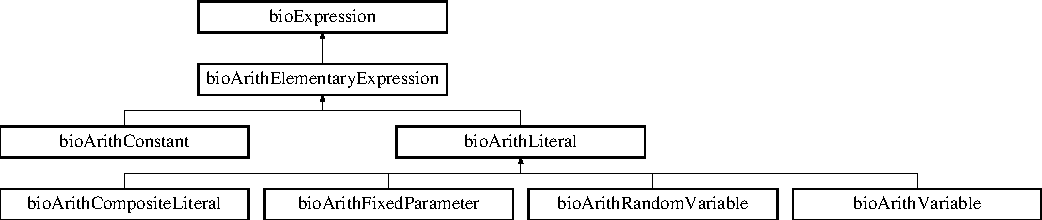
\includegraphics[height=2.962963cm]{classbio_arith_elementary_expression}
\end{center}
\end{figure}
\subsection*{Public Member Functions}
\begin{DoxyCompactItemize}
\item 
\mbox{\Hypertarget{classbio_arith_elementary_expression_a7e6fce4a237dae9d0a002273f1144c0f}\label{classbio_arith_elementary_expression_a7e6fce4a237dae9d0a002273f1144c0f}} 
{\bfseries bio\+Arith\+Elementary\+Expression} (\hyperlink{classbio_expression_repository}{bio\+Expression\+Repository} $\ast$rep, pat\+U\+Long par)
\item 
\mbox{\Hypertarget{classbio_arith_elementary_expression_ad0580d3a2ab21f301a131e187ee504f3}\label{classbio_arith_elementary_expression_ad0580d3a2ab21f301a131e187ee504f3}} 
virtual pat\+U\+Long {\bfseries get\+Number\+Of\+Operations} () const
\item 
\mbox{\Hypertarget{classbio_arith_elementary_expression_a5c1548f90e0ce54653c7b319ed260c2e}\label{classbio_arith_elementary_expression_a5c1548f90e0ce54653c7b319ed260c2e}} 
virtual pat\+Boolean {\bfseries contains\+An\+Iterator} () const
\item 
\mbox{\Hypertarget{classbio_arith_elementary_expression_aaea78451d997c2b3b3e911e93118d4d1}\label{classbio_arith_elementary_expression_aaea78451d997c2b3b3e911e93118d4d1}} 
virtual pat\+Boolean {\bfseries contains\+An\+Iterator\+On\+Rows} () const
\item 
\mbox{\Hypertarget{classbio_arith_elementary_expression_aa994776430d8af57c9e964ce296e8da1}\label{classbio_arith_elementary_expression_aa994776430d8af57c9e964ce296e8da1}} 
virtual pat\+Boolean {\bfseries contains\+An\+Integral} () const
\item 
\mbox{\Hypertarget{classbio_arith_elementary_expression_ac7326fe2e8d9396cd56e45219be0867e}\label{classbio_arith_elementary_expression_ac7326fe2e8d9396cd56e45219be0867e}} 
virtual pat\+Boolean {\bfseries contains\+A\+Sequence} () const
\item 
virtual pat\+String \hyperlink{classbio_arith_elementary_expression_a9293635c83789f547b5642855f8c8f16}{get\+Expression} (pat\+Error $\ast$\&err) const
\item 
\mbox{\Hypertarget{classbio_arith_elementary_expression_a17e6a689c2b513c05460693f7328376b}\label{classbio_arith_elementary_expression_a17e6a689c2b513c05460693f7328376b}} 
virtual \hyperlink{classbio_expression}{bio\+Expression} $\ast$ {\bfseries get\+Expression\+From\+Id} (pat\+U\+Long the\+Id)
\item 
\mbox{\Hypertarget{classbio_arith_elementary_expression_a8f87ed84536747d5f8fe3e69773f621f}\label{classbio_arith_elementary_expression_a8f87ed84536747d5f8fe3e69773f621f}} 
virtual void {\bfseries simplify\+Zeros} (pat\+Error $\ast$\&err)
\item 
\mbox{\Hypertarget{classbio_arith_elementary_expression_ae9d4c3a08a93fce0c901edf19638eedd}\label{classbio_arith_elementary_expression_ae9d4c3a08a93fce0c901edf19638eedd}} 
virtual void {\bfseries collect\+Expression\+Ids} (set$<$ pat\+U\+Long $>$ $\ast$s) const
\item 
\mbox{\Hypertarget{classbio_arith_elementary_expression_acfb07ccdaf1d39f91e3cdeda4c9c076a}\label{classbio_arith_elementary_expression_acfb07ccdaf1d39f91e3cdeda4c9c076a}} 
virtual pat\+String {\bfseries check} (pat\+Error $\ast$\&err) const
\end{DoxyCompactItemize}
\subsection*{Additional Inherited Members}


\subsection{Detailed Description}
Class implementing a node of the tree representing an elementary expression, without any chil 

\subsection{Member Function Documentation}
\mbox{\Hypertarget{classbio_arith_elementary_expression_a9293635c83789f547b5642855f8c8f16}\label{classbio_arith_elementary_expression_a9293635c83789f547b5642855f8c8f16}} 
\index{bio\+Arith\+Elementary\+Expression@{bio\+Arith\+Elementary\+Expression}!get\+Expression@{get\+Expression}}
\index{get\+Expression@{get\+Expression}!bio\+Arith\+Elementary\+Expression@{bio\+Arith\+Elementary\+Expression}}
\subsubsection{\texorpdfstring{get\+Expression()}{getExpression()}}
{\footnotesize\ttfamily pat\+String bio\+Arith\+Elementary\+Expression\+::get\+Expression (\begin{DoxyParamCaption}\item[{pat\+Error $\ast$\&}]{err }\end{DoxyParamCaption}) const\hspace{0.3cm}{\ttfamily [virtual]}}

\begin{DoxyReturn}{Returns}
printed expression 
\end{DoxyReturn}


Reimplemented from \hyperlink{classbio_expression_a66a83eb0caac18dd5e568ffde5a8b5d4}{bio\+Expression}.



Reimplemented in \hyperlink{classbio_arith_constant_a50fd07c61fc6674c05f23345b972807c}{bio\+Arith\+Constant}, and \hyperlink{classbio_arith_literal_ae55e7cbd7d3561b56af50fc741009a60}{bio\+Arith\+Literal}.



The documentation for this class was generated from the following files\+:\begin{DoxyCompactItemize}
\item 
bio\+Arith\+Elementary\+Expression.\+h\item 
bio\+Arith\+Elementary\+Expression.\+cc\end{DoxyCompactItemize}

\hypertarget{classbio_arith_equal}{}\section{bio\+Arith\+Equal Class Reference}
\label{classbio_arith_equal}\index{bio\+Arith\+Equal@{bio\+Arith\+Equal}}


{\ttfamily \#include $<$bio\+Arith\+Equal.\+h$>$}

Inheritance diagram for bio\+Arith\+Equal\+:\begin{figure}[H]
\begin{center}
\leavevmode
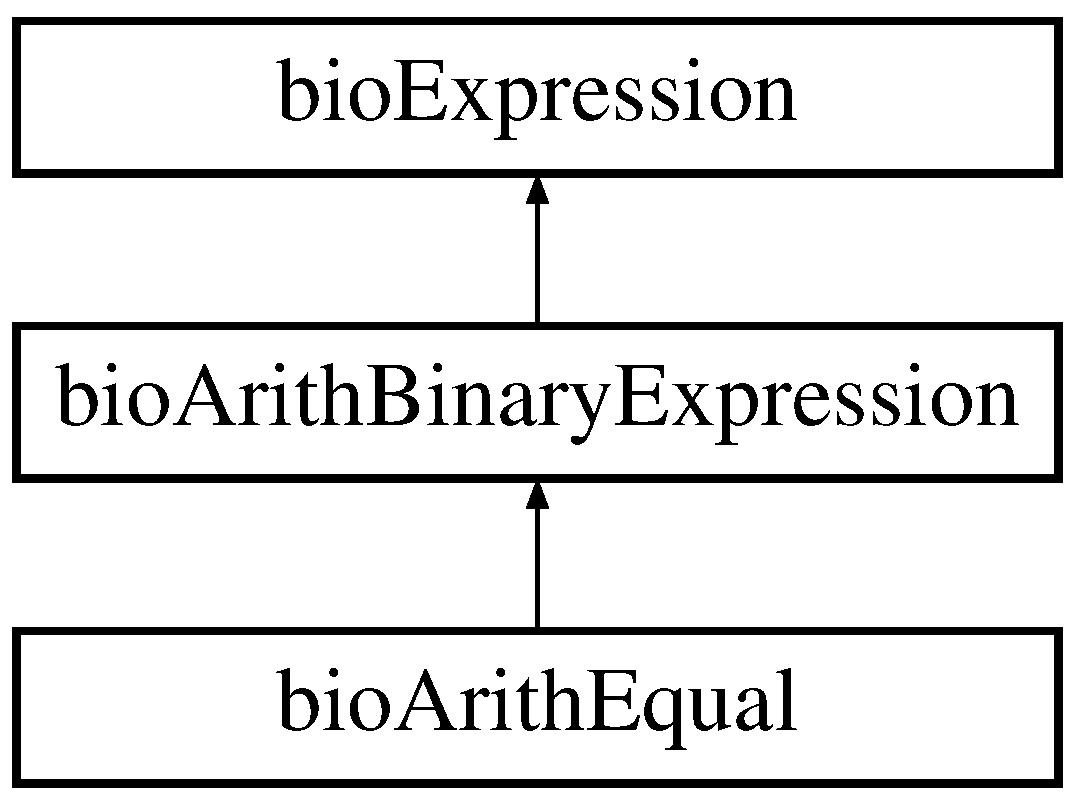
\includegraphics[height=3.000000cm]{classbio_arith_equal}
\end{center}
\end{figure}
\subsection*{Public Member Functions}
\begin{DoxyCompactItemize}
\item 
\mbox{\Hypertarget{classbio_arith_equal_a081112a3f17041cf4f7c5da396cddc10}\label{classbio_arith_equal_a081112a3f17041cf4f7c5da396cddc10}} 
{\bfseries bio\+Arith\+Equal} (\hyperlink{classbio_expression_repository}{bio\+Expression\+Repository} $\ast$rep, pat\+U\+Long par, pat\+U\+Long left, pat\+U\+Long right, pat\+Error $\ast$\&err)
\item 
virtual pat\+String \hyperlink{classbio_arith_equal_ab4a9657d32f37ab61fbe2597b3c4b9eb}{get\+Operator\+Name} () const
\item 
virtual pat\+Real \hyperlink{classbio_arith_equal_a7db4558e7e275cdf8cb525a23d7dac28}{get\+Value} (pat\+Boolean prepare\+Gradient, pat\+U\+Long current\+Lap, pat\+Error $\ast$\&err)
\item 
virtual \hyperlink{classbio_expression}{bio\+Expression} $\ast$ \hyperlink{classbio_arith_equal_a91d4c7481582a8a039dc373eddc707b8}{get\+Derivative} (pat\+U\+Long a\+Literal\+Id, pat\+Error $\ast$\&err) const
\item 
virtual \hyperlink{classbio_arith_equal}{bio\+Arith\+Equal} $\ast$ \hyperlink{classbio_arith_equal_a01b4bf9f63da99bf1ef17c518d2f6eab}{get\+Deep\+Copy} (\hyperlink{classbio_expression_repository}{bio\+Expression\+Repository} $\ast$rep, pat\+Error $\ast$\&err) const
\item 
virtual \hyperlink{classbio_arith_equal}{bio\+Arith\+Equal} $\ast$ \hyperlink{classbio_arith_equal_ace5ebcd053feb9fa4a7e97920fdfe030}{get\+Shallow\+Copy} (\hyperlink{classbio_expression_repository}{bio\+Expression\+Repository} $\ast$rep, pat\+Error $\ast$\&err) const
\item 
virtual pat\+String \hyperlink{classbio_arith_equal_a69839ab065a8bd3d9d0409fbd529c22e}{get\+Expression\+String} () const
\item 
virtual \hyperlink{classbio_function_and_derivatives}{bio\+Function\+And\+Derivatives} $\ast$ \hyperlink{classbio_arith_equal_a9462014bd44ab537c4e6d631a46e97b7}{get\+Numerical\+Function\+And\+Gradient} (vector$<$ pat\+U\+Long $>$ literal\+Ids, pat\+Boolean compute\+Hessian, pat\+Boolean debug\+Derivatives, pat\+Error $\ast$\&err)
\end{DoxyCompactItemize}
\subsection*{Additional Inherited Members}


\subsection{Detailed Description}
Class implementing a node of the tree representing a comparison (==) operation 

\subsection{Member Function Documentation}
\mbox{\Hypertarget{classbio_arith_equal_a01b4bf9f63da99bf1ef17c518d2f6eab}\label{classbio_arith_equal_a01b4bf9f63da99bf1ef17c518d2f6eab}} 
\index{bio\+Arith\+Equal@{bio\+Arith\+Equal}!get\+Deep\+Copy@{get\+Deep\+Copy}}
\index{get\+Deep\+Copy@{get\+Deep\+Copy}!bio\+Arith\+Equal@{bio\+Arith\+Equal}}
\subsubsection{\texorpdfstring{get\+Deep\+Copy()}{getDeepCopy()}}
{\footnotesize\ttfamily \hyperlink{classbio_arith_equal}{bio\+Arith\+Equal} $\ast$ bio\+Arith\+Equal\+::get\+Deep\+Copy (\begin{DoxyParamCaption}\item[{\hyperlink{classbio_expression_repository}{bio\+Expression\+Repository} $\ast$}]{rep,  }\item[{pat\+Error $\ast$\&}]{err }\end{DoxyParamCaption}) const\hspace{0.3cm}{\ttfamily [virtual]}}

Create a deep copy of the expression and returns a pointer to it. It means that new instances of the children are created. 

Reimplemented from \hyperlink{classbio_expression_a4ee1b8add634078a02eaae26cd40dcc8}{bio\+Expression}.

\mbox{\Hypertarget{classbio_arith_equal_a91d4c7481582a8a039dc373eddc707b8}\label{classbio_arith_equal_a91d4c7481582a8a039dc373eddc707b8}} 
\index{bio\+Arith\+Equal@{bio\+Arith\+Equal}!get\+Derivative@{get\+Derivative}}
\index{get\+Derivative@{get\+Derivative}!bio\+Arith\+Equal@{bio\+Arith\+Equal}}
\subsubsection{\texorpdfstring{get\+Derivative()}{getDerivative()}}
{\footnotesize\ttfamily \hyperlink{classbio_expression}{bio\+Expression} $\ast$ bio\+Arith\+Equal\+::get\+Derivative (\begin{DoxyParamCaption}\item[{pat\+U\+Long}]{a\+Literal\+Id,  }\item[{pat\+Error $\ast$\&}]{err }\end{DoxyParamCaption}) const\hspace{0.3cm}{\ttfamily [virtual]}}

\begin{DoxyReturn}{Returns}
value of the derivative w.\+r.\+t literal 
\end{DoxyReturn}

\begin{DoxyParams}{Parameters}
{\em index} & of the literal involved in the derivative \\
\hline
{\em err} & ref. of the pointer to the error object. \\
\hline
\end{DoxyParams}


Reimplemented from \hyperlink{classbio_expression_a5915579d1193f25f216c1e273c97f2ce}{bio\+Expression}.

\mbox{\Hypertarget{classbio_arith_equal_a69839ab065a8bd3d9d0409fbd529c22e}\label{classbio_arith_equal_a69839ab065a8bd3d9d0409fbd529c22e}} 
\index{bio\+Arith\+Equal@{bio\+Arith\+Equal}!get\+Expression\+String@{get\+Expression\+String}}
\index{get\+Expression\+String@{get\+Expression\+String}!bio\+Arith\+Equal@{bio\+Arith\+Equal}}
\subsubsection{\texorpdfstring{get\+Expression\+String()}{getExpressionString()}}
{\footnotesize\ttfamily pat\+String bio\+Arith\+Equal\+::get\+Expression\+String (\begin{DoxyParamCaption}{ }\end{DoxyParamCaption}) const\hspace{0.3cm}{\ttfamily [virtual]}}

Compute a string that represents the expression. It is designed to replace the expression itself when used only for comparison purposes. Code\+: +\{expr1\}\{expr2\}\+: binary plus -\/\{expr1\}\{expr2\}\+: binary minus \{expr1\}\{expr2\}\+: multiplication /\{expr1\}\{expr2\}\+: division $^\wedge$\{expr1\}\{expr2\}\+: power \&\{expr1\}\{expr2\}\+: and $\vert$\{expr1\}\{expr2\}\+: or =\{expr1\}\{expr2\}\+: equal !=\{expr1\}\{expr2\}\+: not equal $<$\{expr1\}\{expr2\}\+: lesser than $<$=\{expr1\}\{expr2\}\+: lesser or equal to $>$\{expr1\}\{expr2\}\+: greater than $>$=\{expr1\}\{expr2\}\+: greater or equal to \$A\{expr\}\+: abs \$D\mbox{[}expr\mbox{]}\mbox{[}\{expr1\}...\{exprN\}\mbox{]}\+: dictionary (\hyperlink{classbio_arith_elem}{bio\+Arith\+Elem}) \$E\{expr\}\+: exp \$L\{expr\}\+: log \$M\{expr\}\+: Unary minus \$\+Piterator\+\_\+name\{expr\}\+: prod \$Q\{string1\}\{string2\}\+: sequence \$\+Siterator\+\_\+name\{expr\}\+: sum \$\+Ziterator\+\_\+name\mbox{[}\{expr1\}...\{exprN\}\mbox{]}\+: merged sum \{expr1\}\{expr2\}...\{exprN\}//\+: list of expressions number\+: constant \#id\+: literal \&id\+: random 

Reimplemented from \hyperlink{classbio_expression_a3e4b4dca58dbbc6f0e411b30eb3f60b4}{bio\+Expression}.

\mbox{\Hypertarget{classbio_arith_equal_a9462014bd44ab537c4e6d631a46e97b7}\label{classbio_arith_equal_a9462014bd44ab537c4e6d631a46e97b7}} 
\index{bio\+Arith\+Equal@{bio\+Arith\+Equal}!get\+Numerical\+Function\+And\+Gradient@{get\+Numerical\+Function\+And\+Gradient}}
\index{get\+Numerical\+Function\+And\+Gradient@{get\+Numerical\+Function\+And\+Gradient}!bio\+Arith\+Equal@{bio\+Arith\+Equal}}
\subsubsection{\texorpdfstring{get\+Numerical\+Function\+And\+Gradient()}{getNumericalFunctionAndGradient()}}
{\footnotesize\ttfamily \hyperlink{classbio_function_and_derivatives}{bio\+Function\+And\+Derivatives} $\ast$ bio\+Arith\+Equal\+::get\+Numerical\+Function\+And\+Gradient (\begin{DoxyParamCaption}\item[{vector$<$ pat\+U\+Long $>$}]{literal\+Ids,  }\item[{pat\+Boolean}]{compute\+Hessian,  }\item[{pat\+Boolean}]{debug\+Derivatives,  }\item[{pat\+Error $\ast$\&}]{err }\end{DoxyParamCaption})\hspace{0.3cm}{\ttfamily [virtual]}}

\begin{DoxyReturn}{Returns}
value and gradient of the expression 
\end{DoxyReturn}

\begin{DoxyParams}{Parameters}
{\em err} & ref. of the pointer to the error object. \\
\hline
\end{DoxyParams}


Reimplemented from \hyperlink{classbio_expression_a91c81ce80c9e972c913b10f5f3c1ed13}{bio\+Expression}.

\mbox{\Hypertarget{classbio_arith_equal_ab4a9657d32f37ab61fbe2597b3c4b9eb}\label{classbio_arith_equal_ab4a9657d32f37ab61fbe2597b3c4b9eb}} 
\index{bio\+Arith\+Equal@{bio\+Arith\+Equal}!get\+Operator\+Name@{get\+Operator\+Name}}
\index{get\+Operator\+Name@{get\+Operator\+Name}!bio\+Arith\+Equal@{bio\+Arith\+Equal}}
\subsubsection{\texorpdfstring{get\+Operator\+Name()}{getOperatorName()}}
{\footnotesize\ttfamily pat\+String bio\+Arith\+Equal\+::get\+Operator\+Name (\begin{DoxyParamCaption}{ }\end{DoxyParamCaption}) const\hspace{0.3cm}{\ttfamily [virtual]}}

\begin{DoxyReturn}{Returns}
name of the operator 
\end{DoxyReturn}


Reimplemented from \hyperlink{classbio_expression_a2353a4afb3a2b0af7c63aba086a72bde}{bio\+Expression}.

\mbox{\Hypertarget{classbio_arith_equal_ace5ebcd053feb9fa4a7e97920fdfe030}\label{classbio_arith_equal_ace5ebcd053feb9fa4a7e97920fdfe030}} 
\index{bio\+Arith\+Equal@{bio\+Arith\+Equal}!get\+Shallow\+Copy@{get\+Shallow\+Copy}}
\index{get\+Shallow\+Copy@{get\+Shallow\+Copy}!bio\+Arith\+Equal@{bio\+Arith\+Equal}}
\subsubsection{\texorpdfstring{get\+Shallow\+Copy()}{getShallowCopy()}}
{\footnotesize\ttfamily \hyperlink{classbio_arith_equal}{bio\+Arith\+Equal} $\ast$ bio\+Arith\+Equal\+::get\+Shallow\+Copy (\begin{DoxyParamCaption}\item[{\hyperlink{classbio_expression_repository}{bio\+Expression\+Repository} $\ast$}]{rep,  }\item[{pat\+Error $\ast$\&}]{err }\end{DoxyParamCaption}) const\hspace{0.3cm}{\ttfamily [virtual]}}

Create a shallow copy of the expression and returns a pointer to it. It means that no new instance of the children are created. It is typically called by the repository 

Reimplemented from \hyperlink{classbio_expression_a442534762693b92baaf33928979a1bf8}{bio\+Expression}.

\mbox{\Hypertarget{classbio_arith_equal_a7db4558e7e275cdf8cb525a23d7dac28}\label{classbio_arith_equal_a7db4558e7e275cdf8cb525a23d7dac28}} 
\index{bio\+Arith\+Equal@{bio\+Arith\+Equal}!get\+Value@{get\+Value}}
\index{get\+Value@{get\+Value}!bio\+Arith\+Equal@{bio\+Arith\+Equal}}
\subsubsection{\texorpdfstring{get\+Value()}{getValue()}}
{\footnotesize\ttfamily pat\+Real bio\+Arith\+Equal\+::get\+Value (\begin{DoxyParamCaption}\item[{pat\+Boolean}]{prepare\+Gradient,  }\item[{pat\+U\+Long}]{current\+Lap,  }\item[{pat\+Error $\ast$\&}]{err }\end{DoxyParamCaption})\hspace{0.3cm}{\ttfamily [virtual]}}

\begin{DoxyReturn}{Returns}
value of the expression 
\end{DoxyReturn}

\begin{DoxyParams}{Parameters}
{\em err} & ref. of the pointer to the error object. \\
\hline
\end{DoxyParams}


Reimplemented from \hyperlink{classbio_expression_af58662a5d4d456f15bc4f2c9bd4f8a5b}{bio\+Expression}.



The documentation for this class was generated from the following files\+:\begin{DoxyCompactItemize}
\item 
bio\+Arith\+Equal.\+h\item 
bio\+Arith\+Equal.\+cc\end{DoxyCompactItemize}

\hypertarget{classbio_arith_exp}{}\section{bio\+Arith\+Exp Class Reference}
\label{classbio_arith_exp}\index{bio\+Arith\+Exp@{bio\+Arith\+Exp}}


{\ttfamily \#include $<$bio\+Arith\+Exp.\+h$>$}

Inheritance diagram for bio\+Arith\+Exp\+:\begin{figure}[H]
\begin{center}
\leavevmode
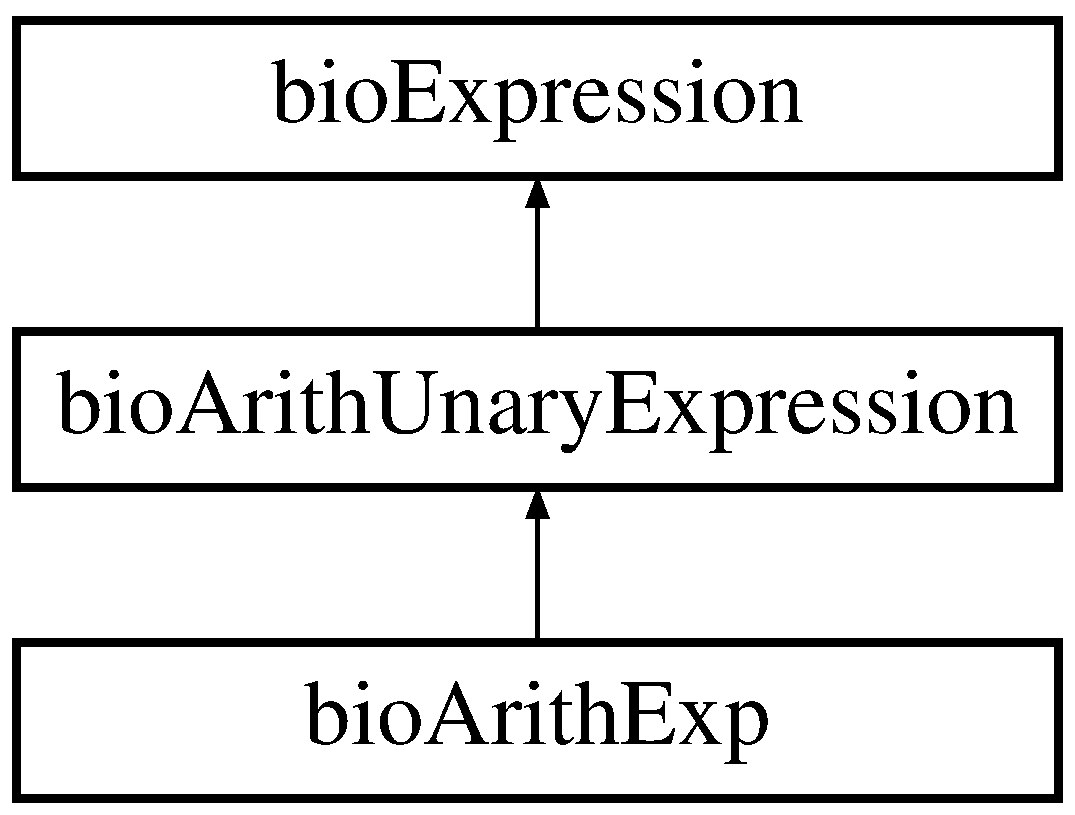
\includegraphics[height=3.000000cm]{classbio_arith_exp}
\end{center}
\end{figure}
\subsection*{Public Member Functions}
\begin{DoxyCompactItemize}
\item 
\mbox{\Hypertarget{classbio_arith_exp_a7cd34e21bc0f74b09a59d4c44e489c4c}\label{classbio_arith_exp_a7cd34e21bc0f74b09a59d4c44e489c4c}} 
{\bfseries bio\+Arith\+Exp} (\hyperlink{classbio_expression_repository}{bio\+Expression\+Repository} $\ast$rep, pat\+U\+Long par, pat\+U\+Long left, pat\+Error $\ast$\&err)
\item 
virtual pat\+String \hyperlink{classbio_arith_exp_a968d5d3d908d11da745e5c680ae981f9}{get\+Operator\+Name} () const
\item 
virtual pat\+Real \hyperlink{classbio_arith_exp_a291d459eb5a41df1ac6409420a8a5713}{get\+Value} (pat\+Boolean prepare\+Gradient, pat\+U\+Long current\+Lap, pat\+Error $\ast$\&err)
\item 
virtual \hyperlink{classbio_expression}{bio\+Expression} $\ast$ \hyperlink{classbio_arith_exp_ae6fb9aa47399f18af66cb4250b36f707}{get\+Derivative} (pat\+U\+Long a\+Literal\+Id, pat\+Error $\ast$\&err) const
\item 
virtual \hyperlink{classbio_arith_exp}{bio\+Arith\+Exp} $\ast$ \hyperlink{classbio_arith_exp_aec1900d14fe80411c3322358773c7ac6}{get\+Deep\+Copy} (\hyperlink{classbio_expression_repository}{bio\+Expression\+Repository} $\ast$rep, pat\+Error $\ast$\&err) const
\item 
virtual \hyperlink{classbio_arith_exp}{bio\+Arith\+Exp} $\ast$ \hyperlink{classbio_arith_exp_a3d2f7448252ebfb7133a3eeef866bea4}{get\+Shallow\+Copy} (\hyperlink{classbio_expression_repository}{bio\+Expression\+Repository} $\ast$rep, pat\+Error $\ast$\&err) const
\item 
virtual pat\+String \hyperlink{classbio_arith_exp_a3bf86cc33d7879bdf4e9e420890f6851}{get\+Expression\+String} () const
\item 
virtual \hyperlink{classbio_function_and_derivatives}{bio\+Function\+And\+Derivatives} $\ast$ \hyperlink{classbio_arith_exp_ab470a2671ba4ed891cd13c621d197fe1}{get\+Numerical\+Function\+And\+Gradient} (vector$<$ pat\+U\+Long $>$ literal\+Ids, pat\+Boolean compute\+Hessian, pat\+Boolean debug\+Derivatives, pat\+Error $\ast$\&err)
\end{DoxyCompactItemize}
\subsection*{Additional Inherited Members}


\subsection{Detailed Description}
Class implementing a node of the tree representing an exponential operation 

\subsection{Member Function Documentation}
\mbox{\Hypertarget{classbio_arith_exp_aec1900d14fe80411c3322358773c7ac6}\label{classbio_arith_exp_aec1900d14fe80411c3322358773c7ac6}} 
\index{bio\+Arith\+Exp@{bio\+Arith\+Exp}!get\+Deep\+Copy@{get\+Deep\+Copy}}
\index{get\+Deep\+Copy@{get\+Deep\+Copy}!bio\+Arith\+Exp@{bio\+Arith\+Exp}}
\subsubsection{\texorpdfstring{get\+Deep\+Copy()}{getDeepCopy()}}
{\footnotesize\ttfamily \hyperlink{classbio_arith_exp}{bio\+Arith\+Exp} $\ast$ bio\+Arith\+Exp\+::get\+Deep\+Copy (\begin{DoxyParamCaption}\item[{\hyperlink{classbio_expression_repository}{bio\+Expression\+Repository} $\ast$}]{rep,  }\item[{pat\+Error $\ast$\&}]{err }\end{DoxyParamCaption}) const\hspace{0.3cm}{\ttfamily [virtual]}}

Create a deep copy of the expression and returns a pointer to it. It means that new instances of the children are created. 

Reimplemented from \hyperlink{classbio_expression_a4ee1b8add634078a02eaae26cd40dcc8}{bio\+Expression}.

\mbox{\Hypertarget{classbio_arith_exp_ae6fb9aa47399f18af66cb4250b36f707}\label{classbio_arith_exp_ae6fb9aa47399f18af66cb4250b36f707}} 
\index{bio\+Arith\+Exp@{bio\+Arith\+Exp}!get\+Derivative@{get\+Derivative}}
\index{get\+Derivative@{get\+Derivative}!bio\+Arith\+Exp@{bio\+Arith\+Exp}}
\subsubsection{\texorpdfstring{get\+Derivative()}{getDerivative()}}
{\footnotesize\ttfamily \hyperlink{classbio_expression}{bio\+Expression} $\ast$ bio\+Arith\+Exp\+::get\+Derivative (\begin{DoxyParamCaption}\item[{pat\+U\+Long}]{a\+Literal\+Id,  }\item[{pat\+Error $\ast$\&}]{err }\end{DoxyParamCaption}) const\hspace{0.3cm}{\ttfamily [virtual]}}

\begin{DoxyReturn}{Returns}
value of the derivative w.\+r.\+t literal 
\end{DoxyReturn}

\begin{DoxyParams}{Parameters}
{\em index} & of the literal involved in the derivative \\
\hline
{\em err} & ref. of the pointer to the error object. \\
\hline
\end{DoxyParams}


Reimplemented from \hyperlink{classbio_expression_a5915579d1193f25f216c1e273c97f2ce}{bio\+Expression}.

\mbox{\Hypertarget{classbio_arith_exp_a3bf86cc33d7879bdf4e9e420890f6851}\label{classbio_arith_exp_a3bf86cc33d7879bdf4e9e420890f6851}} 
\index{bio\+Arith\+Exp@{bio\+Arith\+Exp}!get\+Expression\+String@{get\+Expression\+String}}
\index{get\+Expression\+String@{get\+Expression\+String}!bio\+Arith\+Exp@{bio\+Arith\+Exp}}
\subsubsection{\texorpdfstring{get\+Expression\+String()}{getExpressionString()}}
{\footnotesize\ttfamily pat\+String bio\+Arith\+Exp\+::get\+Expression\+String (\begin{DoxyParamCaption}{ }\end{DoxyParamCaption}) const\hspace{0.3cm}{\ttfamily [virtual]}}

Compute a string that represents the expression. It is designed to replace the expression itself when used only for comparison purposes. Code\+: +\{expr1\}\{expr2\}\+: binary plus -\/\{expr1\}\{expr2\}\+: binary minus \{expr1\}\{expr2\}\+: multiplication /\{expr1\}\{expr2\}\+: division $^\wedge$\{expr1\}\{expr2\}\+: power \&\{expr1\}\{expr2\}\+: and $\vert$\{expr1\}\{expr2\}\+: or =\{expr1\}\{expr2\}\+: equal !=\{expr1\}\{expr2\}\+: not equal $<$\{expr1\}\{expr2\}\+: lesser than $<$=\{expr1\}\{expr2\}\+: lesser or equal to $>$\{expr1\}\{expr2\}\+: greater than $>$=\{expr1\}\{expr2\}\+: greater or equal to \$A\{expr\}\+: abs \$D\mbox{[}expr\mbox{]}\mbox{[}\{expr1\}...\{exprN\}\mbox{]}\+: dictionary (\hyperlink{classbio_arith_elem}{bio\+Arith\+Elem}) \$E\{expr\}\+: exp \$L\{expr\}\+: log \$M\{expr\}\+: Unary minus \$\+Piterator\+\_\+name\{expr\}\+: prod \$Q\{string1\}\{string2\}\+: sequence \$\+Siterator\+\_\+name\{expr\}\+: sum \$\+Ziterator\+\_\+name\mbox{[}\{expr1\}...\{exprN\}\mbox{]}\+: merged sum \{expr1\}\{expr2\}...\{exprN\}//\+: list of expressions number\+: constant \#id\+: literal \&id\+: random 

Reimplemented from \hyperlink{classbio_expression_a3e4b4dca58dbbc6f0e411b30eb3f60b4}{bio\+Expression}.

\mbox{\Hypertarget{classbio_arith_exp_ab470a2671ba4ed891cd13c621d197fe1}\label{classbio_arith_exp_ab470a2671ba4ed891cd13c621d197fe1}} 
\index{bio\+Arith\+Exp@{bio\+Arith\+Exp}!get\+Numerical\+Function\+And\+Gradient@{get\+Numerical\+Function\+And\+Gradient}}
\index{get\+Numerical\+Function\+And\+Gradient@{get\+Numerical\+Function\+And\+Gradient}!bio\+Arith\+Exp@{bio\+Arith\+Exp}}
\subsubsection{\texorpdfstring{get\+Numerical\+Function\+And\+Gradient()}{getNumericalFunctionAndGradient()}}
{\footnotesize\ttfamily \hyperlink{classbio_function_and_derivatives}{bio\+Function\+And\+Derivatives} $\ast$ bio\+Arith\+Exp\+::get\+Numerical\+Function\+And\+Gradient (\begin{DoxyParamCaption}\item[{vector$<$ pat\+U\+Long $>$}]{literal\+Ids,  }\item[{pat\+Boolean}]{compute\+Hessian,  }\item[{pat\+Boolean}]{debug\+Derivatives,  }\item[{pat\+Error $\ast$\&}]{err }\end{DoxyParamCaption})\hspace{0.3cm}{\ttfamily [virtual]}}

\begin{DoxyReturn}{Returns}
value and gradient of the expression 
\end{DoxyReturn}

\begin{DoxyParams}{Parameters}
{\em err} & ref. of the pointer to the error object. \\
\hline
\end{DoxyParams}


Reimplemented from \hyperlink{classbio_expression_a91c81ce80c9e972c913b10f5f3c1ed13}{bio\+Expression}.

\mbox{\Hypertarget{classbio_arith_exp_a968d5d3d908d11da745e5c680ae981f9}\label{classbio_arith_exp_a968d5d3d908d11da745e5c680ae981f9}} 
\index{bio\+Arith\+Exp@{bio\+Arith\+Exp}!get\+Operator\+Name@{get\+Operator\+Name}}
\index{get\+Operator\+Name@{get\+Operator\+Name}!bio\+Arith\+Exp@{bio\+Arith\+Exp}}
\subsubsection{\texorpdfstring{get\+Operator\+Name()}{getOperatorName()}}
{\footnotesize\ttfamily pat\+String bio\+Arith\+Exp\+::get\+Operator\+Name (\begin{DoxyParamCaption}{ }\end{DoxyParamCaption}) const\hspace{0.3cm}{\ttfamily [virtual]}}

\begin{DoxyReturn}{Returns}
name of the operator 
\end{DoxyReturn}


Reimplemented from \hyperlink{classbio_expression_a2353a4afb3a2b0af7c63aba086a72bde}{bio\+Expression}.

\mbox{\Hypertarget{classbio_arith_exp_a3d2f7448252ebfb7133a3eeef866bea4}\label{classbio_arith_exp_a3d2f7448252ebfb7133a3eeef866bea4}} 
\index{bio\+Arith\+Exp@{bio\+Arith\+Exp}!get\+Shallow\+Copy@{get\+Shallow\+Copy}}
\index{get\+Shallow\+Copy@{get\+Shallow\+Copy}!bio\+Arith\+Exp@{bio\+Arith\+Exp}}
\subsubsection{\texorpdfstring{get\+Shallow\+Copy()}{getShallowCopy()}}
{\footnotesize\ttfamily \hyperlink{classbio_arith_exp}{bio\+Arith\+Exp} $\ast$ bio\+Arith\+Exp\+::get\+Shallow\+Copy (\begin{DoxyParamCaption}\item[{\hyperlink{classbio_expression_repository}{bio\+Expression\+Repository} $\ast$}]{rep,  }\item[{pat\+Error $\ast$\&}]{err }\end{DoxyParamCaption}) const\hspace{0.3cm}{\ttfamily [virtual]}}

Create a shallow copy of the expression and returns a pointer to it. It means that no new instance of the children are created. It is typically called by the repository 

Reimplemented from \hyperlink{classbio_expression_a442534762693b92baaf33928979a1bf8}{bio\+Expression}.

\mbox{\Hypertarget{classbio_arith_exp_a291d459eb5a41df1ac6409420a8a5713}\label{classbio_arith_exp_a291d459eb5a41df1ac6409420a8a5713}} 
\index{bio\+Arith\+Exp@{bio\+Arith\+Exp}!get\+Value@{get\+Value}}
\index{get\+Value@{get\+Value}!bio\+Arith\+Exp@{bio\+Arith\+Exp}}
\subsubsection{\texorpdfstring{get\+Value()}{getValue()}}
{\footnotesize\ttfamily pat\+Real bio\+Arith\+Exp\+::get\+Value (\begin{DoxyParamCaption}\item[{pat\+Boolean}]{prepare\+Gradient,  }\item[{pat\+U\+Long}]{current\+Lap,  }\item[{pat\+Error $\ast$\&}]{err }\end{DoxyParamCaption})\hspace{0.3cm}{\ttfamily [virtual]}}

\begin{DoxyReturn}{Returns}
value of the expression 
\end{DoxyReturn}

\begin{DoxyParams}{Parameters}
{\em err} & ref. of the pointer to the error object. \\
\hline
\end{DoxyParams}


Reimplemented from \hyperlink{classbio_expression_af58662a5d4d456f15bc4f2c9bd4f8a5b}{bio\+Expression}.



The documentation for this class was generated from the following files\+:\begin{DoxyCompactItemize}
\item 
bio\+Arith\+Exp.\+h\item 
bio\+Arith\+Exp.\+cc\end{DoxyCompactItemize}

\hypertarget{classbio_arith_fixed_parameter}{}\section{bio\+Arith\+Fixed\+Parameter Class Reference}
\label{classbio_arith_fixed_parameter}\index{bio\+Arith\+Fixed\+Parameter@{bio\+Arith\+Fixed\+Parameter}}


{\ttfamily \#include $<$bio\+Arith\+Fixed\+Parameter.\+h$>$}

Inheritance diagram for bio\+Arith\+Fixed\+Parameter\+:\begin{figure}[H]
\begin{center}
\leavevmode
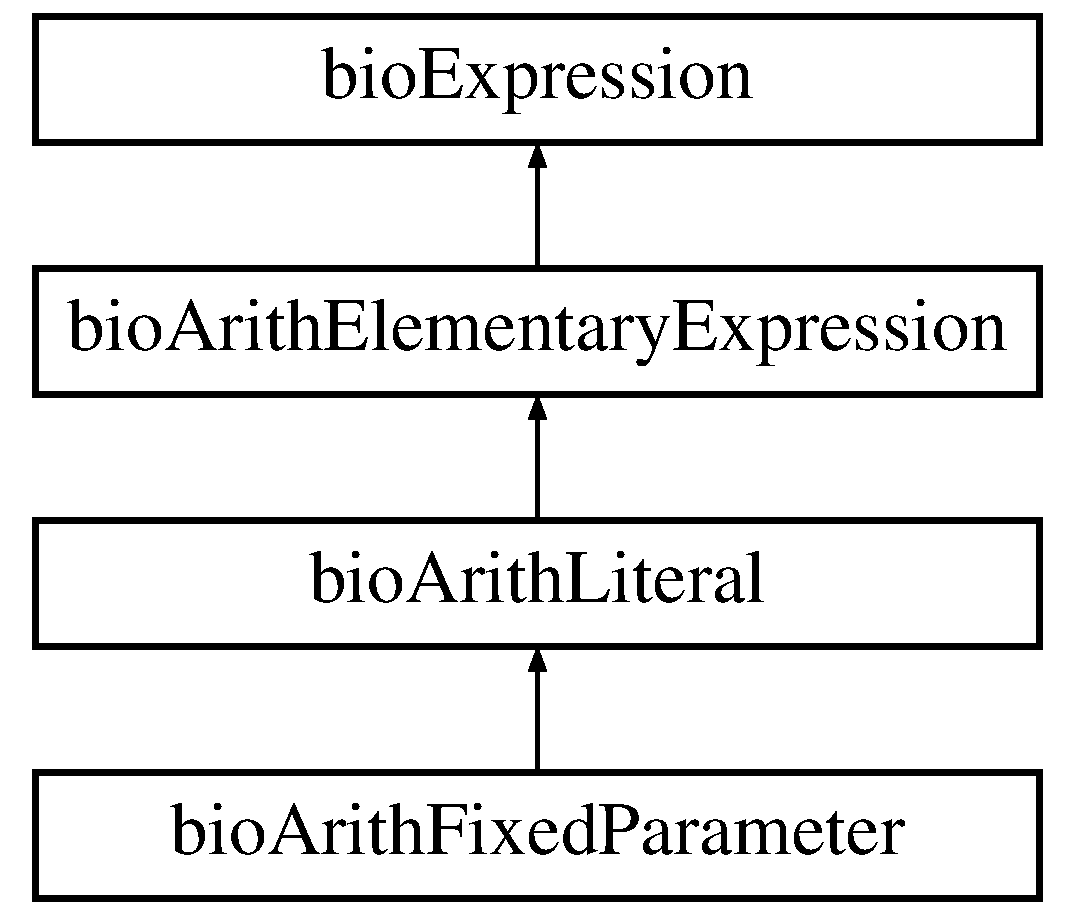
\includegraphics[height=4.000000cm]{classbio_arith_fixed_parameter}
\end{center}
\end{figure}
\subsection*{Public Member Functions}
\begin{DoxyCompactItemize}
\item 
\mbox{\Hypertarget{classbio_arith_fixed_parameter_a80ea6a846533ac52342c48712bc997d2}\label{classbio_arith_fixed_parameter_a80ea6a846533ac52342c48712bc997d2}} 
{\bfseries bio\+Arith\+Fixed\+Parameter} (\hyperlink{classbio_expression_repository}{bio\+Expression\+Repository} $\ast$rep, pat\+U\+Long par, pat\+U\+Long unique\+Id, pat\+U\+Long b\+Id)
\item 
virtual \hyperlink{classbio_arith_fixed_parameter}{bio\+Arith\+Fixed\+Parameter} $\ast$ \hyperlink{classbio_arith_fixed_parameter_a91c2dcaf2be8731defb45a02108b7b82}{get\+Deep\+Copy} (\hyperlink{classbio_expression_repository}{bio\+Expression\+Repository} $\ast$rep, pat\+Error $\ast$\&err) const
\item 
virtual \hyperlink{classbio_arith_fixed_parameter}{bio\+Arith\+Fixed\+Parameter} $\ast$ \hyperlink{classbio_arith_fixed_parameter_a0743b72d00d4f769ec3c01faae8ebac8}{get\+Shallow\+Copy} (\hyperlink{classbio_expression_repository}{bio\+Expression\+Repository} $\ast$rep, pat\+Error $\ast$\&err) const
\item 
virtual pat\+Real \hyperlink{classbio_arith_fixed_parameter_a0eed9a884a07681f00da9b42e559cd8c}{get\+Value} (pat\+Boolean prepare\+Gradient, pat\+U\+Long current\+Lap, pat\+Error $\ast$\&err)
\end{DoxyCompactItemize}
\subsection*{Protected Attributes}
\begin{DoxyCompactItemize}
\item 
\mbox{\Hypertarget{classbio_arith_fixed_parameter_a237d0536be87836417ca0c94db93a986}\label{classbio_arith_fixed_parameter_a237d0536be87836417ca0c94db93a986}} 
pat\+U\+Long {\bfseries the\+Parameter\+Id}
\item 
\mbox{\Hypertarget{classbio_arith_fixed_parameter_a22ef22b4b158871dc8f7cf6b3b5171de}\label{classbio_arith_fixed_parameter_a22ef22b4b158871dc8f7cf6b3b5171de}} 
const \hyperlink{classbio_fixed_parameter}{bio\+Fixed\+Parameter} $\ast$ {\bfseries the\+Parameter}
\end{DoxyCompactItemize}


\subsection{Detailed Description}
Class implementing the node for variables in an expression 

\subsection{Member Function Documentation}
\mbox{\Hypertarget{classbio_arith_fixed_parameter_a91c2dcaf2be8731defb45a02108b7b82}\label{classbio_arith_fixed_parameter_a91c2dcaf2be8731defb45a02108b7b82}} 
\index{bio\+Arith\+Fixed\+Parameter@{bio\+Arith\+Fixed\+Parameter}!get\+Deep\+Copy@{get\+Deep\+Copy}}
\index{get\+Deep\+Copy@{get\+Deep\+Copy}!bio\+Arith\+Fixed\+Parameter@{bio\+Arith\+Fixed\+Parameter}}
\subsubsection{\texorpdfstring{get\+Deep\+Copy()}{getDeepCopy()}}
{\footnotesize\ttfamily \hyperlink{classbio_arith_fixed_parameter}{bio\+Arith\+Fixed\+Parameter} $\ast$ bio\+Arith\+Fixed\+Parameter\+::get\+Deep\+Copy (\begin{DoxyParamCaption}\item[{\hyperlink{classbio_expression_repository}{bio\+Expression\+Repository} $\ast$}]{rep,  }\item[{pat\+Error $\ast$\&}]{err }\end{DoxyParamCaption}) const\hspace{0.3cm}{\ttfamily [virtual]}}

Create a deep copy of the expression and returns a pointer to it. It means that new instances of the children are created. 

Reimplemented from \hyperlink{classbio_expression_a4ee1b8add634078a02eaae26cd40dcc8}{bio\+Expression}.

\mbox{\Hypertarget{classbio_arith_fixed_parameter_a0743b72d00d4f769ec3c01faae8ebac8}\label{classbio_arith_fixed_parameter_a0743b72d00d4f769ec3c01faae8ebac8}} 
\index{bio\+Arith\+Fixed\+Parameter@{bio\+Arith\+Fixed\+Parameter}!get\+Shallow\+Copy@{get\+Shallow\+Copy}}
\index{get\+Shallow\+Copy@{get\+Shallow\+Copy}!bio\+Arith\+Fixed\+Parameter@{bio\+Arith\+Fixed\+Parameter}}
\subsubsection{\texorpdfstring{get\+Shallow\+Copy()}{getShallowCopy()}}
{\footnotesize\ttfamily \hyperlink{classbio_arith_fixed_parameter}{bio\+Arith\+Fixed\+Parameter} $\ast$ bio\+Arith\+Fixed\+Parameter\+::get\+Shallow\+Copy (\begin{DoxyParamCaption}\item[{\hyperlink{classbio_expression_repository}{bio\+Expression\+Repository} $\ast$}]{rep,  }\item[{pat\+Error $\ast$\&}]{err }\end{DoxyParamCaption}) const\hspace{0.3cm}{\ttfamily [virtual]}}

Create a shallow copy of the expression and returns a pointer to it. It means that no new instance of the children are created. It is typically called by the repository 

Reimplemented from \hyperlink{classbio_expression_a442534762693b92baaf33928979a1bf8}{bio\+Expression}.

\mbox{\Hypertarget{classbio_arith_fixed_parameter_a0eed9a884a07681f00da9b42e559cd8c}\label{classbio_arith_fixed_parameter_a0eed9a884a07681f00da9b42e559cd8c}} 
\index{bio\+Arith\+Fixed\+Parameter@{bio\+Arith\+Fixed\+Parameter}!get\+Value@{get\+Value}}
\index{get\+Value@{get\+Value}!bio\+Arith\+Fixed\+Parameter@{bio\+Arith\+Fixed\+Parameter}}
\subsubsection{\texorpdfstring{get\+Value()}{getValue()}}
{\footnotesize\ttfamily pat\+Real bio\+Arith\+Fixed\+Parameter\+::get\+Value (\begin{DoxyParamCaption}\item[{pat\+Boolean}]{prepare\+Gradient,  }\item[{pat\+U\+Long}]{current\+Lap,  }\item[{pat\+Error $\ast$\&}]{err }\end{DoxyParamCaption})\hspace{0.3cm}{\ttfamily [virtual]}}

\begin{DoxyReturn}{Returns}
value of the expression 
\end{DoxyReturn}

\begin{DoxyParams}{Parameters}
{\em err} & ref. of the pointer to the error object. \\
\hline
\end{DoxyParams}


Reimplemented from \hyperlink{classbio_expression_af58662a5d4d456f15bc4f2c9bd4f8a5b}{bio\+Expression}.



The documentation for this class was generated from the following files\+:\begin{DoxyCompactItemize}
\item 
bio\+Arith\+Fixed\+Parameter.\+h\item 
bio\+Arith\+Fixed\+Parameter.\+cc\end{DoxyCompactItemize}

\hypertarget{classbio_arith_gauss_hermite}{}\section{bio\+Arith\+Gauss\+Hermite Class Reference}
\label{classbio_arith_gauss_hermite}\index{bio\+Arith\+Gauss\+Hermite@{bio\+Arith\+Gauss\+Hermite}}
Inheritance diagram for bio\+Arith\+Gauss\+Hermite\+:\begin{figure}[H]
\begin{center}
\leavevmode
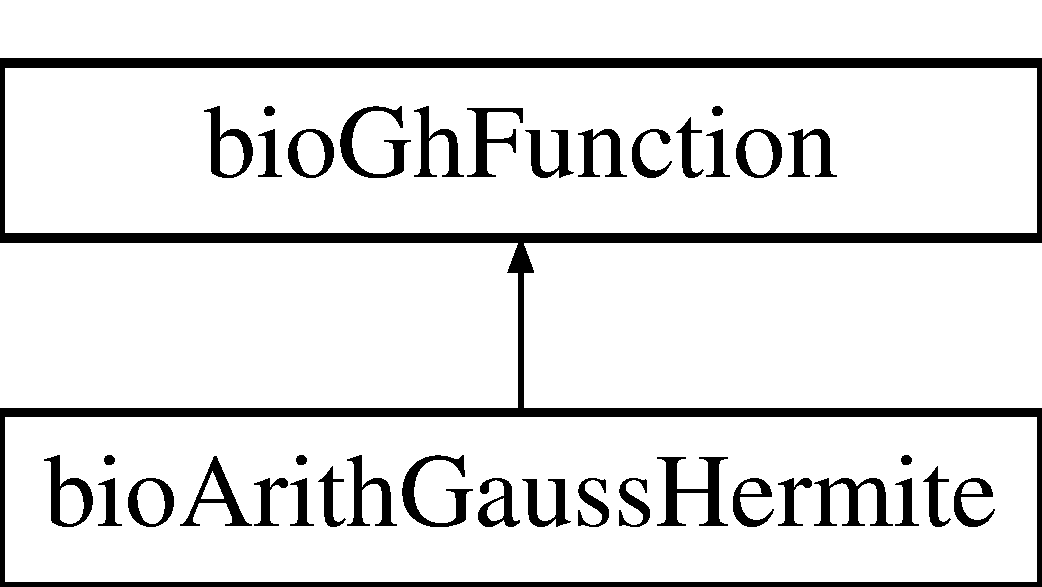
\includegraphics[height=2.000000cm]{classbio_arith_gauss_hermite}
\end{center}
\end{figure}
\subsection*{Public Member Functions}
\begin{DoxyCompactItemize}
\item 
\mbox{\Hypertarget{classbio_arith_gauss_hermite_a6c79acf4e8a09c8427801b89110bcce8}\label{classbio_arith_gauss_hermite_a6c79acf4e8a09c8427801b89110bcce8}} 
{\bfseries bio\+Arith\+Gauss\+Hermite} (\hyperlink{classbio_expression}{bio\+Expression} $\ast$e, vector$<$ pat\+U\+Long $>$ derivl, pat\+U\+Long l, pat\+Boolean wg, pat\+Boolean wh)
\item 
\mbox{\Hypertarget{classbio_arith_gauss_hermite_a31be90b1b21fc19969058b9997ff8f50}\label{classbio_arith_gauss_hermite_a31be90b1b21fc19969058b9997ff8f50}} 
vector$<$ pat\+Real $>$ {\bfseries get\+Value} (pat\+Real x, pat\+Error $\ast$\&err)
\item 
\mbox{\Hypertarget{classbio_arith_gauss_hermite_a3e656c295515a681ed169be28e9f9ab5}\label{classbio_arith_gauss_hermite_a3e656c295515a681ed169be28e9f9ab5}} 
pat\+U\+Long {\bfseries get\+Size} () const
\item 
\mbox{\Hypertarget{classbio_arith_gauss_hermite_ab7b78ce3bf66f31a3803511cfa91f39d}\label{classbio_arith_gauss_hermite_ab7b78ce3bf66f31a3803511cfa91f39d}} 
pat\+U\+Long {\bfseries get\+Thread\+Id} () const
\end{DoxyCompactItemize}


The documentation for this class was generated from the following files\+:\begin{DoxyCompactItemize}
\item 
bio\+Arith\+Gauss\+Hermite.\+h\item 
bio\+Arith\+Gauss\+Hermite.\+cc\end{DoxyCompactItemize}

\hypertarget{classbio_arith_g_h_integral}{}\section{bio\+Arith\+G\+H\+Integral Class Reference}
\label{classbio_arith_g_h_integral}\index{bio\+Arith\+G\+H\+Integral@{bio\+Arith\+G\+H\+Integral}}


{\ttfamily \#include $<$bio\+Arith\+G\+H\+Integral.\+h$>$}

Inheritance diagram for bio\+Arith\+G\+H\+Integral\+:\begin{figure}[H]
\begin{center}
\leavevmode
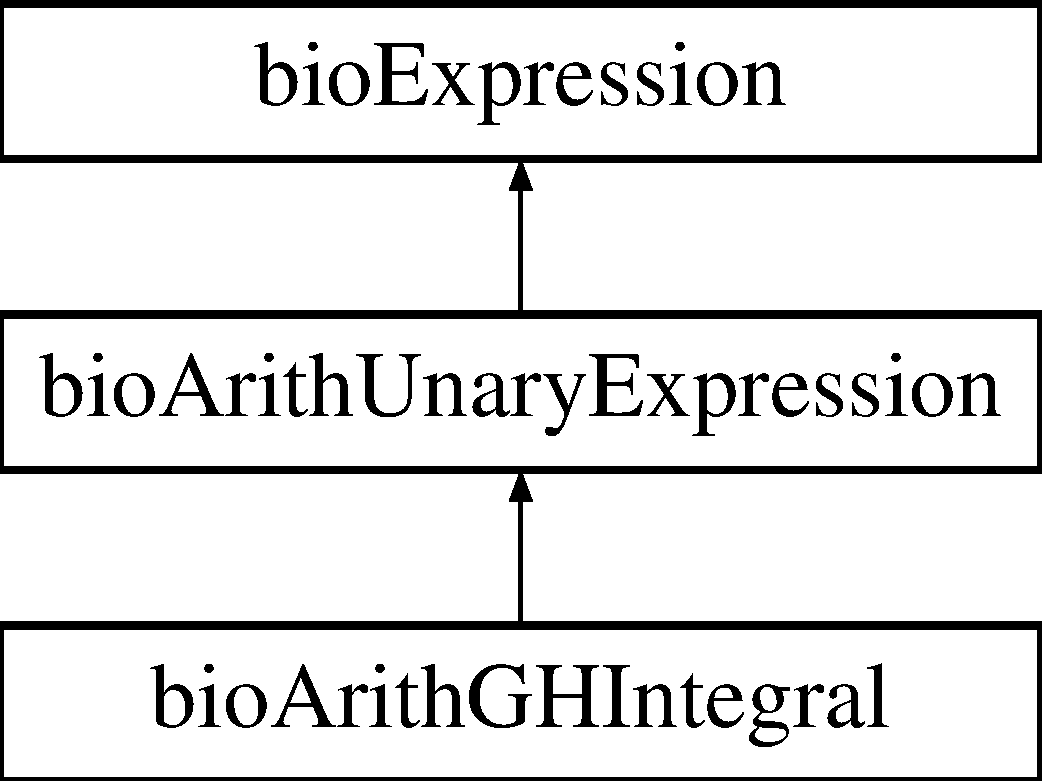
\includegraphics[height=3.000000cm]{classbio_arith_g_h_integral}
\end{center}
\end{figure}
\subsection*{Public Member Functions}
\begin{DoxyCompactItemize}
\item 
\mbox{\Hypertarget{classbio_arith_g_h_integral_a01934487b2480803d990b9575c19ef2a}\label{classbio_arith_g_h_integral_a01934487b2480803d990b9575c19ef2a}} 
{\bfseries bio\+Arith\+G\+H\+Integral} (\hyperlink{classbio_expression_repository}{bio\+Expression\+Repository} $\ast$rep, pat\+U\+Long par, pat\+U\+Long left, pat\+String a\+Literal\+Name, pat\+Error $\ast$\&err)
\item 
virtual pat\+String \hyperlink{classbio_arith_g_h_integral_a2eeabe5fdedaee0370596b34d7731b77}{get\+Operator\+Name} () const
\item 
virtual pat\+Real \hyperlink{classbio_arith_g_h_integral_a6eecafaf8d88fc08dfc8c4feb2d68ffd}{get\+Value} (pat\+Boolean prepare\+Gradient, pat\+U\+Long current\+Lap, pat\+Error $\ast$\&err)
\item 
virtual \hyperlink{classbio_expression}{bio\+Expression} $\ast$ \hyperlink{classbio_arith_g_h_integral_a3e017f569acbc481366ad4472ee2734d}{get\+Derivative} (pat\+U\+Long a\+Literal\+Id, pat\+Error $\ast$\&err) const
\item 
virtual \hyperlink{classbio_arith_g_h_integral}{bio\+Arith\+G\+H\+Integral} $\ast$ \hyperlink{classbio_arith_g_h_integral_a4864f99351baa9b168451d2356d2e7bf}{get\+Deep\+Copy} (\hyperlink{classbio_expression_repository}{bio\+Expression\+Repository} $\ast$rep, pat\+Error $\ast$\&err) const
\item 
virtual \hyperlink{classbio_arith_g_h_integral}{bio\+Arith\+G\+H\+Integral} $\ast$ \hyperlink{classbio_arith_g_h_integral_a15d9820a85bd45e3643c6bd15752cfe2}{get\+Shallow\+Copy} (\hyperlink{classbio_expression_repository}{bio\+Expression\+Repository} $\ast$rep, pat\+Error $\ast$\&err) const
\item 
virtual pat\+Boolean \hyperlink{classbio_arith_g_h_integral_a86510e9d5d13234c931278ec496e1aec}{is\+Structurally\+Zero} () const
\item 
virtual pat\+String \hyperlink{classbio_arith_g_h_integral_aa245fc792bcd733e143896c9f8d33a64}{get\+Expression\+String} () const
\item 
virtual \hyperlink{classbio_function_and_derivatives}{bio\+Function\+And\+Derivatives} $\ast$ \hyperlink{classbio_arith_g_h_integral_a2148674c32e7bea35d7e6ef275c2f7f5}{get\+Numerical\+Function\+And\+Gradient} (vector$<$ pat\+U\+Long $>$ literal\+Ids, pat\+Boolean compute\+Hessian, pat\+Boolean debug\+Derivatives, pat\+Error $\ast$\&err)
\end{DoxyCompactItemize}
\subsection*{Public Attributes}
\begin{DoxyCompactItemize}
\item 
\mbox{\Hypertarget{classbio_arith_g_h_integral_a0f454f8bb154996248767e5d91ffcfe0}\label{classbio_arith_g_h_integral_a0f454f8bb154996248767e5d91ffcfe0}} 
pat\+U\+Long {\bfseries literal\+Id}
\item 
\mbox{\Hypertarget{classbio_arith_g_h_integral_abd269a8e70436ad0c429c8b910cbd877}\label{classbio_arith_g_h_integral_abd269a8e70436ad0c429c8b910cbd877}} 
pat\+String {\bfseries literal\+Name}
\end{DoxyCompactItemize}
\subsection*{Additional Inherited Members}


\subsection{Detailed Description}
Class implementing a node of the tree representing an integral between -\/infty and +infty 

\subsection{Member Function Documentation}
\mbox{\Hypertarget{classbio_arith_g_h_integral_a4864f99351baa9b168451d2356d2e7bf}\label{classbio_arith_g_h_integral_a4864f99351baa9b168451d2356d2e7bf}} 
\index{bio\+Arith\+G\+H\+Integral@{bio\+Arith\+G\+H\+Integral}!get\+Deep\+Copy@{get\+Deep\+Copy}}
\index{get\+Deep\+Copy@{get\+Deep\+Copy}!bio\+Arith\+G\+H\+Integral@{bio\+Arith\+G\+H\+Integral}}
\subsubsection{\texorpdfstring{get\+Deep\+Copy()}{getDeepCopy()}}
{\footnotesize\ttfamily \hyperlink{classbio_arith_g_h_integral}{bio\+Arith\+G\+H\+Integral} $\ast$ bio\+Arith\+G\+H\+Integral\+::get\+Deep\+Copy (\begin{DoxyParamCaption}\item[{\hyperlink{classbio_expression_repository}{bio\+Expression\+Repository} $\ast$}]{rep,  }\item[{pat\+Error $\ast$\&}]{err }\end{DoxyParamCaption}) const\hspace{0.3cm}{\ttfamily [virtual]}}

Create a deep copy of the expression and returns a pointer to it. It means that new instances of the children are created. 

Reimplemented from \hyperlink{classbio_expression_a4ee1b8add634078a02eaae26cd40dcc8}{bio\+Expression}.

\mbox{\Hypertarget{classbio_arith_g_h_integral_a3e017f569acbc481366ad4472ee2734d}\label{classbio_arith_g_h_integral_a3e017f569acbc481366ad4472ee2734d}} 
\index{bio\+Arith\+G\+H\+Integral@{bio\+Arith\+G\+H\+Integral}!get\+Derivative@{get\+Derivative}}
\index{get\+Derivative@{get\+Derivative}!bio\+Arith\+G\+H\+Integral@{bio\+Arith\+G\+H\+Integral}}
\subsubsection{\texorpdfstring{get\+Derivative()}{getDerivative()}}
{\footnotesize\ttfamily \hyperlink{classbio_expression}{bio\+Expression} $\ast$ bio\+Arith\+G\+H\+Integral\+::get\+Derivative (\begin{DoxyParamCaption}\item[{pat\+U\+Long}]{a\+Literal\+Id,  }\item[{pat\+Error $\ast$\&}]{err }\end{DoxyParamCaption}) const\hspace{0.3cm}{\ttfamily [virtual]}}

\begin{DoxyReturn}{Returns}
value of the derivative w.\+r.\+t literal 
\end{DoxyReturn}

\begin{DoxyParams}{Parameters}
{\em index} & of the literal involved in the derivative \\
\hline
{\em err} & ref. of the pointer to the error object. \\
\hline
\end{DoxyParams}


Reimplemented from \hyperlink{classbio_expression_a5915579d1193f25f216c1e273c97f2ce}{bio\+Expression}.

\mbox{\Hypertarget{classbio_arith_g_h_integral_aa245fc792bcd733e143896c9f8d33a64}\label{classbio_arith_g_h_integral_aa245fc792bcd733e143896c9f8d33a64}} 
\index{bio\+Arith\+G\+H\+Integral@{bio\+Arith\+G\+H\+Integral}!get\+Expression\+String@{get\+Expression\+String}}
\index{get\+Expression\+String@{get\+Expression\+String}!bio\+Arith\+G\+H\+Integral@{bio\+Arith\+G\+H\+Integral}}
\subsubsection{\texorpdfstring{get\+Expression\+String()}{getExpressionString()}}
{\footnotesize\ttfamily pat\+String bio\+Arith\+G\+H\+Integral\+::get\+Expression\+String (\begin{DoxyParamCaption}{ }\end{DoxyParamCaption}) const\hspace{0.3cm}{\ttfamily [virtual]}}

Compute a string that represents the expression. It is designed to replace the expression itself when used only for comparison purposes. Code\+: +\{expr1\}\{expr2\}\+: binary plus -\/\{expr1\}\{expr2\}\+: binary minus \{expr1\}\{expr2\}\+: multiplication /\{expr1\}\{expr2\}\+: division $^\wedge$\{expr1\}\{expr2\}\+: power \&\{expr1\}\{expr2\}\+: and $\vert$\{expr1\}\{expr2\}\+: or =\{expr1\}\{expr2\}\+: equal !=\{expr1\}\{expr2\}\+: not equal $<$\{expr1\}\{expr2\}\+: lesser than $<$=\{expr1\}\{expr2\}\+: lesser or equal to $>$\{expr1\}\{expr2\}\+: greater than $>$=\{expr1\}\{expr2\}\+: greater or equal to \$A\{expr\}\+: abs \$D\mbox{[}expr\mbox{]}\mbox{[}\{expr1\}...\{exprN\}\mbox{]}\+: dictionary (\hyperlink{classbio_arith_elem}{bio\+Arith\+Elem}) \$E\{expr\}\+: exp \$L\{expr\}\+: log \$M\{expr\}\+: Unary minus \$\+Piterator\+\_\+name\{expr\}\+: prod \$Q\{string1\}\{string2\}\+: sequence \$\+Siterator\+\_\+name\{expr\}\+: sum \$\+Ziterator\+\_\+name\mbox{[}\{expr1\}...\{exprN\}\mbox{]}\+: merged sum \{expr1\}\{expr2\}...\{exprN\}//\+: list of expressions number\+: constant \#id\+: literal \&id\+: random 

Reimplemented from \hyperlink{classbio_expression_a3e4b4dca58dbbc6f0e411b30eb3f60b4}{bio\+Expression}.

\mbox{\Hypertarget{classbio_arith_g_h_integral_a2148674c32e7bea35d7e6ef275c2f7f5}\label{classbio_arith_g_h_integral_a2148674c32e7bea35d7e6ef275c2f7f5}} 
\index{bio\+Arith\+G\+H\+Integral@{bio\+Arith\+G\+H\+Integral}!get\+Numerical\+Function\+And\+Gradient@{get\+Numerical\+Function\+And\+Gradient}}
\index{get\+Numerical\+Function\+And\+Gradient@{get\+Numerical\+Function\+And\+Gradient}!bio\+Arith\+G\+H\+Integral@{bio\+Arith\+G\+H\+Integral}}
\subsubsection{\texorpdfstring{get\+Numerical\+Function\+And\+Gradient()}{getNumericalFunctionAndGradient()}}
{\footnotesize\ttfamily \hyperlink{classbio_function_and_derivatives}{bio\+Function\+And\+Derivatives} $\ast$ bio\+Arith\+G\+H\+Integral\+::get\+Numerical\+Function\+And\+Gradient (\begin{DoxyParamCaption}\item[{vector$<$ pat\+U\+Long $>$}]{literal\+Ids,  }\item[{pat\+Boolean}]{compute\+Hessian,  }\item[{pat\+Boolean}]{debug\+Derivatives,  }\item[{pat\+Error $\ast$\&}]{err }\end{DoxyParamCaption})\hspace{0.3cm}{\ttfamily [virtual]}}

\begin{DoxyReturn}{Returns}
value and gradient of the expression 
\end{DoxyReturn}

\begin{DoxyParams}{Parameters}
{\em err} & ref. of the pointer to the error object. \\
\hline
\end{DoxyParams}


Reimplemented from \hyperlink{classbio_expression_a91c81ce80c9e972c913b10f5f3c1ed13}{bio\+Expression}.

\mbox{\Hypertarget{classbio_arith_g_h_integral_a2eeabe5fdedaee0370596b34d7731b77}\label{classbio_arith_g_h_integral_a2eeabe5fdedaee0370596b34d7731b77}} 
\index{bio\+Arith\+G\+H\+Integral@{bio\+Arith\+G\+H\+Integral}!get\+Operator\+Name@{get\+Operator\+Name}}
\index{get\+Operator\+Name@{get\+Operator\+Name}!bio\+Arith\+G\+H\+Integral@{bio\+Arith\+G\+H\+Integral}}
\subsubsection{\texorpdfstring{get\+Operator\+Name()}{getOperatorName()}}
{\footnotesize\ttfamily pat\+String bio\+Arith\+G\+H\+Integral\+::get\+Operator\+Name (\begin{DoxyParamCaption}{ }\end{DoxyParamCaption}) const\hspace{0.3cm}{\ttfamily [virtual]}}

\begin{DoxyReturn}{Returns}
name of the operator 
\end{DoxyReturn}


Reimplemented from \hyperlink{classbio_expression_a2353a4afb3a2b0af7c63aba086a72bde}{bio\+Expression}.

\mbox{\Hypertarget{classbio_arith_g_h_integral_a15d9820a85bd45e3643c6bd15752cfe2}\label{classbio_arith_g_h_integral_a15d9820a85bd45e3643c6bd15752cfe2}} 
\index{bio\+Arith\+G\+H\+Integral@{bio\+Arith\+G\+H\+Integral}!get\+Shallow\+Copy@{get\+Shallow\+Copy}}
\index{get\+Shallow\+Copy@{get\+Shallow\+Copy}!bio\+Arith\+G\+H\+Integral@{bio\+Arith\+G\+H\+Integral}}
\subsubsection{\texorpdfstring{get\+Shallow\+Copy()}{getShallowCopy()}}
{\footnotesize\ttfamily \hyperlink{classbio_arith_g_h_integral}{bio\+Arith\+G\+H\+Integral} $\ast$ bio\+Arith\+G\+H\+Integral\+::get\+Shallow\+Copy (\begin{DoxyParamCaption}\item[{\hyperlink{classbio_expression_repository}{bio\+Expression\+Repository} $\ast$}]{rep,  }\item[{pat\+Error $\ast$\&}]{err }\end{DoxyParamCaption}) const\hspace{0.3cm}{\ttfamily [virtual]}}

Create a shallow copy of the expression and returns a pointer to it. It means that no new instance of the children are created. It is typically called by the repository 

Reimplemented from \hyperlink{classbio_expression_a442534762693b92baaf33928979a1bf8}{bio\+Expression}.

\mbox{\Hypertarget{classbio_arith_g_h_integral_a6eecafaf8d88fc08dfc8c4feb2d68ffd}\label{classbio_arith_g_h_integral_a6eecafaf8d88fc08dfc8c4feb2d68ffd}} 
\index{bio\+Arith\+G\+H\+Integral@{bio\+Arith\+G\+H\+Integral}!get\+Value@{get\+Value}}
\index{get\+Value@{get\+Value}!bio\+Arith\+G\+H\+Integral@{bio\+Arith\+G\+H\+Integral}}
\subsubsection{\texorpdfstring{get\+Value()}{getValue()}}
{\footnotesize\ttfamily pat\+Real bio\+Arith\+G\+H\+Integral\+::get\+Value (\begin{DoxyParamCaption}\item[{pat\+Boolean}]{prepare\+Gradient,  }\item[{pat\+U\+Long}]{current\+Lap,  }\item[{pat\+Error $\ast$\&}]{err }\end{DoxyParamCaption})\hspace{0.3cm}{\ttfamily [virtual]}}

\begin{DoxyReturn}{Returns}
value of the expression 
\end{DoxyReturn}

\begin{DoxyParams}{Parameters}
{\em err} & ref. of the pointer to the error object. \\
\hline
\end{DoxyParams}


Reimplemented from \hyperlink{classbio_expression_af58662a5d4d456f15bc4f2c9bd4f8a5b}{bio\+Expression}.

\mbox{\Hypertarget{classbio_arith_g_h_integral_a86510e9d5d13234c931278ec496e1aec}\label{classbio_arith_g_h_integral_a86510e9d5d13234c931278ec496e1aec}} 
\index{bio\+Arith\+G\+H\+Integral@{bio\+Arith\+G\+H\+Integral}!is\+Structurally\+Zero@{is\+Structurally\+Zero}}
\index{is\+Structurally\+Zero@{is\+Structurally\+Zero}!bio\+Arith\+G\+H\+Integral@{bio\+Arith\+G\+H\+Integral}}
\subsubsection{\texorpdfstring{is\+Structurally\+Zero()}{isStructurallyZero()}}
{\footnotesize\ttfamily pat\+Boolean bio\+Arith\+G\+H\+Integral\+::is\+Structurally\+Zero (\begin{DoxyParamCaption}{ }\end{DoxyParamCaption}) const\hspace{0.3cm}{\ttfamily [virtual]}}

return pat\+T\+R\+UE if the expression is structurally 0 so that there is no need to evaluate it. In the base class, it return pat\+F\+A\+L\+SE. 

Reimplemented from \hyperlink{classbio_expression_a264c6d78671610ada8261d698e4c4c42}{bio\+Expression}.



The documentation for this class was generated from the following files\+:\begin{DoxyCompactItemize}
\item 
bio\+Arith\+G\+H\+Integral.\+h\item 
bio\+Arith\+G\+H\+Integral.\+cc\end{DoxyCompactItemize}

\hypertarget{classbio_arith_greater}{}\section{bio\+Arith\+Greater Class Reference}
\label{classbio_arith_greater}\index{bio\+Arith\+Greater@{bio\+Arith\+Greater}}


{\ttfamily \#include $<$bio\+Arith\+Greater.\+h$>$}

Inheritance diagram for bio\+Arith\+Greater\+:\begin{figure}[H]
\begin{center}
\leavevmode
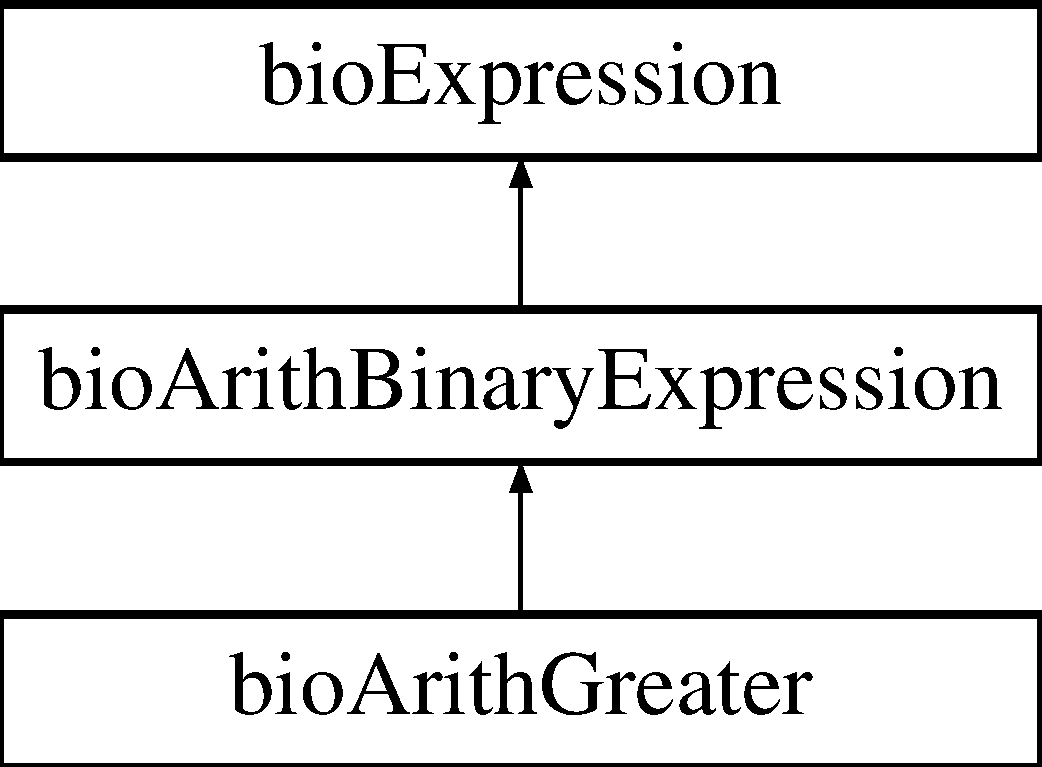
\includegraphics[height=3.000000cm]{classbio_arith_greater}
\end{center}
\end{figure}
\subsection*{Public Member Functions}
\begin{DoxyCompactItemize}
\item 
\mbox{\Hypertarget{classbio_arith_greater_ac62ca926560eead11a14a047d65f0eab}\label{classbio_arith_greater_ac62ca926560eead11a14a047d65f0eab}} 
{\bfseries bio\+Arith\+Greater} (\hyperlink{classbio_expression_repository}{bio\+Expression\+Repository} $\ast$rep, pat\+U\+Long par, pat\+U\+Long left, pat\+U\+Long right, pat\+Error $\ast$\&err)
\item 
virtual pat\+String \hyperlink{classbio_arith_greater_a140169d1d84495e86d21dbd231c14f81}{get\+Operator\+Name} () const
\item 
virtual pat\+Real \hyperlink{classbio_arith_greater_ae486d20a8a8c6cfb1d287bb9de936ddb}{get\+Value} (pat\+Boolean prepare\+Gradient, pat\+U\+Long current\+Lap, pat\+Error $\ast$\&err)
\item 
virtual \hyperlink{classbio_expression}{bio\+Expression} $\ast$ \hyperlink{classbio_arith_greater_a20024dcb6e37aadcdfc7e92c58dc2af3}{get\+Derivative} (pat\+U\+Long a\+Literal\+Id, pat\+Error $\ast$\&err) const
\item 
virtual \hyperlink{classbio_arith_greater}{bio\+Arith\+Greater} $\ast$ \hyperlink{classbio_arith_greater_a39a03806f6465307c2086ce5ae2bed0a}{get\+Deep\+Copy} (\hyperlink{classbio_expression_repository}{bio\+Expression\+Repository} $\ast$rep, pat\+Error $\ast$\&err) const
\item 
virtual \hyperlink{classbio_arith_greater}{bio\+Arith\+Greater} $\ast$ \hyperlink{classbio_arith_greater_a73641032a8328db66db66469573ab61f}{get\+Shallow\+Copy} (\hyperlink{classbio_expression_repository}{bio\+Expression\+Repository} $\ast$rep, pat\+Error $\ast$\&err) const
\item 
virtual pat\+String \hyperlink{classbio_arith_greater_a391651a15d94bbb1cba7bbf74937d3bd}{get\+Expression\+String} () const
\item 
virtual \hyperlink{classbio_function_and_derivatives}{bio\+Function\+And\+Derivatives} $\ast$ \hyperlink{classbio_arith_greater_acd768ff3dd4a85e234cb5fa7b5e1cf91}{get\+Numerical\+Function\+And\+Gradient} (vector$<$ pat\+U\+Long $>$ literal\+Ids, pat\+Boolean compute\+Hessian, pat\+Boolean debug\+Derivatives, pat\+Error $\ast$\&err)
\end{DoxyCompactItemize}
\subsection*{Additional Inherited Members}


\subsection{Detailed Description}
Class implementing a node of the tree representing a comparison ($>$) operation 

\subsection{Member Function Documentation}
\mbox{\Hypertarget{classbio_arith_greater_a39a03806f6465307c2086ce5ae2bed0a}\label{classbio_arith_greater_a39a03806f6465307c2086ce5ae2bed0a}} 
\index{bio\+Arith\+Greater@{bio\+Arith\+Greater}!get\+Deep\+Copy@{get\+Deep\+Copy}}
\index{get\+Deep\+Copy@{get\+Deep\+Copy}!bio\+Arith\+Greater@{bio\+Arith\+Greater}}
\subsubsection{\texorpdfstring{get\+Deep\+Copy()}{getDeepCopy()}}
{\footnotesize\ttfamily \hyperlink{classbio_arith_greater}{bio\+Arith\+Greater} $\ast$ bio\+Arith\+Greater\+::get\+Deep\+Copy (\begin{DoxyParamCaption}\item[{\hyperlink{classbio_expression_repository}{bio\+Expression\+Repository} $\ast$}]{rep,  }\item[{pat\+Error $\ast$\&}]{err }\end{DoxyParamCaption}) const\hspace{0.3cm}{\ttfamily [virtual]}}

Create a deep copy of the expression and returns a pointer to it. It means that new instances of the children are created. 

Reimplemented from \hyperlink{classbio_expression_a4ee1b8add634078a02eaae26cd40dcc8}{bio\+Expression}.

\mbox{\Hypertarget{classbio_arith_greater_a20024dcb6e37aadcdfc7e92c58dc2af3}\label{classbio_arith_greater_a20024dcb6e37aadcdfc7e92c58dc2af3}} 
\index{bio\+Arith\+Greater@{bio\+Arith\+Greater}!get\+Derivative@{get\+Derivative}}
\index{get\+Derivative@{get\+Derivative}!bio\+Arith\+Greater@{bio\+Arith\+Greater}}
\subsubsection{\texorpdfstring{get\+Derivative()}{getDerivative()}}
{\footnotesize\ttfamily \hyperlink{classbio_expression}{bio\+Expression} $\ast$ bio\+Arith\+Greater\+::get\+Derivative (\begin{DoxyParamCaption}\item[{pat\+U\+Long}]{a\+Literal\+Id,  }\item[{pat\+Error $\ast$\&}]{err }\end{DoxyParamCaption}) const\hspace{0.3cm}{\ttfamily [virtual]}}

\begin{DoxyReturn}{Returns}
value of the derivative w.\+r.\+t literal 
\end{DoxyReturn}

\begin{DoxyParams}{Parameters}
{\em index} & of the literal involved in the derivative \\
\hline
{\em err} & ref. of the pointer to the error object. \\
\hline
\end{DoxyParams}


Reimplemented from \hyperlink{classbio_expression_a5915579d1193f25f216c1e273c97f2ce}{bio\+Expression}.

\mbox{\Hypertarget{classbio_arith_greater_a391651a15d94bbb1cba7bbf74937d3bd}\label{classbio_arith_greater_a391651a15d94bbb1cba7bbf74937d3bd}} 
\index{bio\+Arith\+Greater@{bio\+Arith\+Greater}!get\+Expression\+String@{get\+Expression\+String}}
\index{get\+Expression\+String@{get\+Expression\+String}!bio\+Arith\+Greater@{bio\+Arith\+Greater}}
\subsubsection{\texorpdfstring{get\+Expression\+String()}{getExpressionString()}}
{\footnotesize\ttfamily pat\+String bio\+Arith\+Greater\+::get\+Expression\+String (\begin{DoxyParamCaption}{ }\end{DoxyParamCaption}) const\hspace{0.3cm}{\ttfamily [virtual]}}

Compute a string that represents the expression. It is designed to replace the expression itself when used only for comparison purposes. Code\+: +\{expr1\}\{expr2\}\+: binary plus -\/\{expr1\}\{expr2\}\+: binary minus \{expr1\}\{expr2\}\+: multiplication /\{expr1\}\{expr2\}\+: division $^\wedge$\{expr1\}\{expr2\}\+: power \&\{expr1\}\{expr2\}\+: and $\vert$\{expr1\}\{expr2\}\+: or =\{expr1\}\{expr2\}\+: equal !=\{expr1\}\{expr2\}\+: not equal $<$\{expr1\}\{expr2\}\+: lesser than $<$=\{expr1\}\{expr2\}\+: lesser or equal to $>$\{expr1\}\{expr2\}\+: greater than $>$=\{expr1\}\{expr2\}\+: greater or equal to \$A\{expr\}\+: abs \$D\mbox{[}expr\mbox{]}\mbox{[}\{expr1\}...\{exprN\}\mbox{]}\+: dictionary (\hyperlink{classbio_arith_elem}{bio\+Arith\+Elem}) \$E\{expr\}\+: exp \$L\{expr\}\+: log \$M\{expr\}\+: Unary minus \$\+Piterator\+\_\+name\{expr\}\+: prod \$Q\{string1\}\{string2\}\+: sequence \$\+Siterator\+\_\+name\{expr\}\+: sum \$\+Ziterator\+\_\+name\mbox{[}\{expr1\}...\{exprN\}\mbox{]}\+: merged sum \{expr1\}\{expr2\}...\{exprN\}//\+: list of expressions number\+: constant \#id\+: literal \&id\+: random 

Reimplemented from \hyperlink{classbio_expression_a3e4b4dca58dbbc6f0e411b30eb3f60b4}{bio\+Expression}.

\mbox{\Hypertarget{classbio_arith_greater_acd768ff3dd4a85e234cb5fa7b5e1cf91}\label{classbio_arith_greater_acd768ff3dd4a85e234cb5fa7b5e1cf91}} 
\index{bio\+Arith\+Greater@{bio\+Arith\+Greater}!get\+Numerical\+Function\+And\+Gradient@{get\+Numerical\+Function\+And\+Gradient}}
\index{get\+Numerical\+Function\+And\+Gradient@{get\+Numerical\+Function\+And\+Gradient}!bio\+Arith\+Greater@{bio\+Arith\+Greater}}
\subsubsection{\texorpdfstring{get\+Numerical\+Function\+And\+Gradient()}{getNumericalFunctionAndGradient()}}
{\footnotesize\ttfamily \hyperlink{classbio_function_and_derivatives}{bio\+Function\+And\+Derivatives} $\ast$ bio\+Arith\+Greater\+::get\+Numerical\+Function\+And\+Gradient (\begin{DoxyParamCaption}\item[{vector$<$ pat\+U\+Long $>$}]{literal\+Ids,  }\item[{pat\+Boolean}]{compute\+Hessian,  }\item[{pat\+Boolean}]{debug\+Derivatives,  }\item[{pat\+Error $\ast$\&}]{err }\end{DoxyParamCaption})\hspace{0.3cm}{\ttfamily [virtual]}}

\begin{DoxyReturn}{Returns}
value and gradient of the expression 
\end{DoxyReturn}

\begin{DoxyParams}{Parameters}
{\em err} & ref. of the pointer to the error object. \\
\hline
\end{DoxyParams}


Reimplemented from \hyperlink{classbio_expression_a91c81ce80c9e972c913b10f5f3c1ed13}{bio\+Expression}.

\mbox{\Hypertarget{classbio_arith_greater_a140169d1d84495e86d21dbd231c14f81}\label{classbio_arith_greater_a140169d1d84495e86d21dbd231c14f81}} 
\index{bio\+Arith\+Greater@{bio\+Arith\+Greater}!get\+Operator\+Name@{get\+Operator\+Name}}
\index{get\+Operator\+Name@{get\+Operator\+Name}!bio\+Arith\+Greater@{bio\+Arith\+Greater}}
\subsubsection{\texorpdfstring{get\+Operator\+Name()}{getOperatorName()}}
{\footnotesize\ttfamily pat\+String bio\+Arith\+Greater\+::get\+Operator\+Name (\begin{DoxyParamCaption}{ }\end{DoxyParamCaption}) const\hspace{0.3cm}{\ttfamily [virtual]}}

\begin{DoxyReturn}{Returns}
name of the operator 
\end{DoxyReturn}


Reimplemented from \hyperlink{classbio_expression_a2353a4afb3a2b0af7c63aba086a72bde}{bio\+Expression}.

\mbox{\Hypertarget{classbio_arith_greater_a73641032a8328db66db66469573ab61f}\label{classbio_arith_greater_a73641032a8328db66db66469573ab61f}} 
\index{bio\+Arith\+Greater@{bio\+Arith\+Greater}!get\+Shallow\+Copy@{get\+Shallow\+Copy}}
\index{get\+Shallow\+Copy@{get\+Shallow\+Copy}!bio\+Arith\+Greater@{bio\+Arith\+Greater}}
\subsubsection{\texorpdfstring{get\+Shallow\+Copy()}{getShallowCopy()}}
{\footnotesize\ttfamily \hyperlink{classbio_arith_greater}{bio\+Arith\+Greater} $\ast$ bio\+Arith\+Greater\+::get\+Shallow\+Copy (\begin{DoxyParamCaption}\item[{\hyperlink{classbio_expression_repository}{bio\+Expression\+Repository} $\ast$}]{rep,  }\item[{pat\+Error $\ast$\&}]{err }\end{DoxyParamCaption}) const\hspace{0.3cm}{\ttfamily [virtual]}}

Create a shallow copy of the expression and returns a pointer to it. It means that no new instance of the children are created. It is typically called by the repository 

Reimplemented from \hyperlink{classbio_expression_a442534762693b92baaf33928979a1bf8}{bio\+Expression}.

\mbox{\Hypertarget{classbio_arith_greater_ae486d20a8a8c6cfb1d287bb9de936ddb}\label{classbio_arith_greater_ae486d20a8a8c6cfb1d287bb9de936ddb}} 
\index{bio\+Arith\+Greater@{bio\+Arith\+Greater}!get\+Value@{get\+Value}}
\index{get\+Value@{get\+Value}!bio\+Arith\+Greater@{bio\+Arith\+Greater}}
\subsubsection{\texorpdfstring{get\+Value()}{getValue()}}
{\footnotesize\ttfamily pat\+Real bio\+Arith\+Greater\+::get\+Value (\begin{DoxyParamCaption}\item[{pat\+Boolean}]{prepare\+Gradient,  }\item[{pat\+U\+Long}]{current\+Lap,  }\item[{pat\+Error $\ast$\&}]{err }\end{DoxyParamCaption})\hspace{0.3cm}{\ttfamily [virtual]}}

\begin{DoxyReturn}{Returns}
value of the expression 
\end{DoxyReturn}

\begin{DoxyParams}{Parameters}
{\em err} & ref. of the pointer to the error object. \\
\hline
\end{DoxyParams}


Reimplemented from \hyperlink{classbio_expression_af58662a5d4d456f15bc4f2c9bd4f8a5b}{bio\+Expression}.



The documentation for this class was generated from the following files\+:\begin{DoxyCompactItemize}
\item 
bio\+Arith\+Greater.\+h\item 
bio\+Arith\+Greater.\+cc\end{DoxyCompactItemize}

\hypertarget{classbio_arith_greater_equal}{}\section{bio\+Arith\+Greater\+Equal Class Reference}
\label{classbio_arith_greater_equal}\index{bio\+Arith\+Greater\+Equal@{bio\+Arith\+Greater\+Equal}}


{\ttfamily \#include $<$bio\+Arith\+Greater\+Equal.\+h$>$}

Inheritance diagram for bio\+Arith\+Greater\+Equal\+:\begin{figure}[H]
\begin{center}
\leavevmode
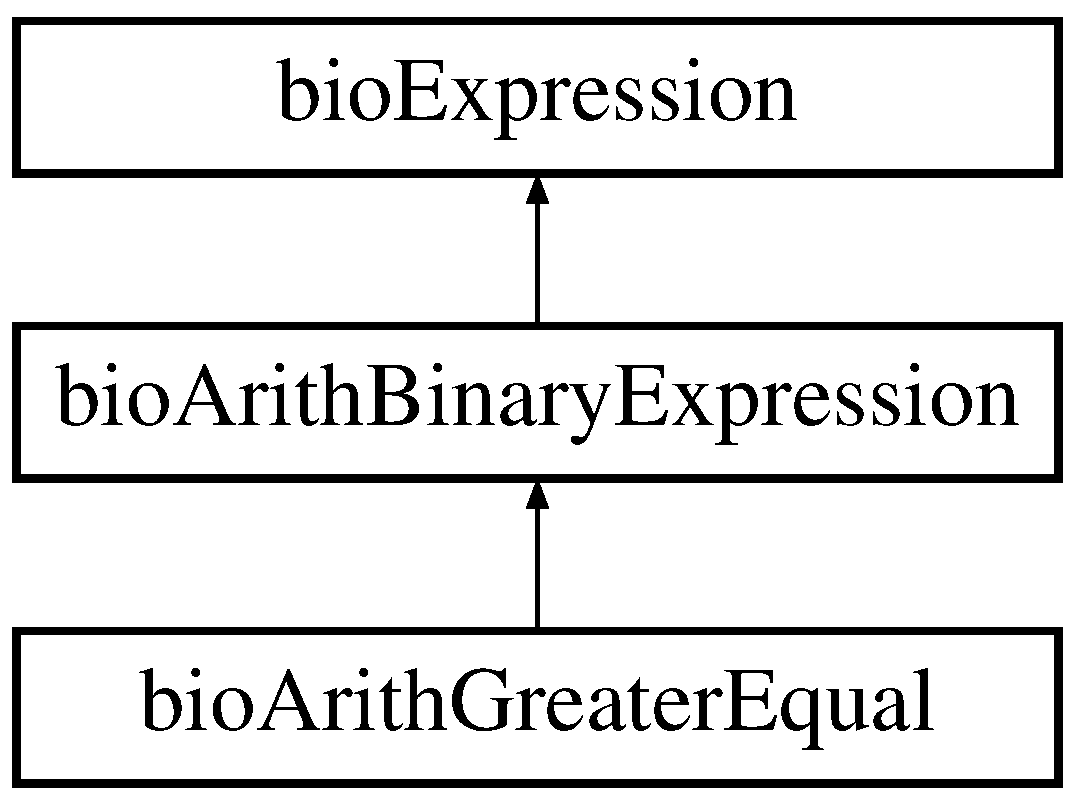
\includegraphics[height=3.000000cm]{classbio_arith_greater_equal}
\end{center}
\end{figure}
\subsection*{Public Member Functions}
\begin{DoxyCompactItemize}
\item 
\mbox{\Hypertarget{classbio_arith_greater_equal_a78e8faa5e1e56babf358b1d795743d01}\label{classbio_arith_greater_equal_a78e8faa5e1e56babf358b1d795743d01}} 
{\bfseries bio\+Arith\+Greater\+Equal} (\hyperlink{classbio_expression_repository}{bio\+Expression\+Repository} $\ast$rep, pat\+U\+Long par, pat\+U\+Long left, pat\+U\+Long right, pat\+Error $\ast$\&err)
\item 
virtual pat\+String \hyperlink{classbio_arith_greater_equal_ab98914bebec6a6dfc6abb9c114a4c7ed}{get\+Operator\+Name} () const
\item 
virtual pat\+Real \hyperlink{classbio_arith_greater_equal_ad9948d07e8c792d998fa6b6099b17633}{get\+Value} (pat\+Boolean prepare\+Gradient, pat\+U\+Long current\+Lap, pat\+Error $\ast$\&err)
\item 
virtual \hyperlink{classbio_expression}{bio\+Expression} $\ast$ \hyperlink{classbio_arith_greater_equal_a6964afaf174b6e1de101f2439e266477}{get\+Derivative} (pat\+U\+Long a\+Literal\+Id, pat\+Error $\ast$\&err) const
\item 
virtual \hyperlink{classbio_arith_greater_equal}{bio\+Arith\+Greater\+Equal} $\ast$ \hyperlink{classbio_arith_greater_equal_aa5ff24eef069374f9c8778ab8569ff7d}{get\+Deep\+Copy} (\hyperlink{classbio_expression_repository}{bio\+Expression\+Repository} $\ast$rep, pat\+Error $\ast$\&err) const
\item 
virtual \hyperlink{classbio_arith_greater_equal}{bio\+Arith\+Greater\+Equal} $\ast$ \hyperlink{classbio_arith_greater_equal_a00fdd329a5be536817f97e532ad29fc5}{get\+Shallow\+Copy} (\hyperlink{classbio_expression_repository}{bio\+Expression\+Repository} $\ast$rep, pat\+Error $\ast$\&err) const
\item 
virtual pat\+String \hyperlink{classbio_arith_greater_equal_a6585da182f8a3cf7063f55be1b68af6c}{get\+Expression\+String} () const
\item 
virtual \hyperlink{classbio_function_and_derivatives}{bio\+Function\+And\+Derivatives} $\ast$ \hyperlink{classbio_arith_greater_equal_aa5ee24b87d59239ca9a0549f72ef8c09}{get\+Numerical\+Function\+And\+Gradient} (vector$<$ pat\+U\+Long $>$ literal\+Ids, pat\+Boolean compute\+Hessian, pat\+Boolean debug\+Derivatives, pat\+Error $\ast$\&err)
\end{DoxyCompactItemize}
\subsection*{Additional Inherited Members}


\subsection{Detailed Description}
Class implementing a node of the tree representing a comparison ($>$=) operation 

\subsection{Member Function Documentation}
\mbox{\Hypertarget{classbio_arith_greater_equal_aa5ff24eef069374f9c8778ab8569ff7d}\label{classbio_arith_greater_equal_aa5ff24eef069374f9c8778ab8569ff7d}} 
\index{bio\+Arith\+Greater\+Equal@{bio\+Arith\+Greater\+Equal}!get\+Deep\+Copy@{get\+Deep\+Copy}}
\index{get\+Deep\+Copy@{get\+Deep\+Copy}!bio\+Arith\+Greater\+Equal@{bio\+Arith\+Greater\+Equal}}
\subsubsection{\texorpdfstring{get\+Deep\+Copy()}{getDeepCopy()}}
{\footnotesize\ttfamily \hyperlink{classbio_arith_greater_equal}{bio\+Arith\+Greater\+Equal} $\ast$ bio\+Arith\+Greater\+Equal\+::get\+Deep\+Copy (\begin{DoxyParamCaption}\item[{\hyperlink{classbio_expression_repository}{bio\+Expression\+Repository} $\ast$}]{rep,  }\item[{pat\+Error $\ast$\&}]{err }\end{DoxyParamCaption}) const\hspace{0.3cm}{\ttfamily [virtual]}}

Create a deep copy of the expression and returns a pointer to it. It means that new instances of the children are created. 

Reimplemented from \hyperlink{classbio_expression_a4ee1b8add634078a02eaae26cd40dcc8}{bio\+Expression}.

\mbox{\Hypertarget{classbio_arith_greater_equal_a6964afaf174b6e1de101f2439e266477}\label{classbio_arith_greater_equal_a6964afaf174b6e1de101f2439e266477}} 
\index{bio\+Arith\+Greater\+Equal@{bio\+Arith\+Greater\+Equal}!get\+Derivative@{get\+Derivative}}
\index{get\+Derivative@{get\+Derivative}!bio\+Arith\+Greater\+Equal@{bio\+Arith\+Greater\+Equal}}
\subsubsection{\texorpdfstring{get\+Derivative()}{getDerivative()}}
{\footnotesize\ttfamily \hyperlink{classbio_expression}{bio\+Expression} $\ast$ bio\+Arith\+Greater\+Equal\+::get\+Derivative (\begin{DoxyParamCaption}\item[{pat\+U\+Long}]{a\+Literal\+Id,  }\item[{pat\+Error $\ast$\&}]{err }\end{DoxyParamCaption}) const\hspace{0.3cm}{\ttfamily [virtual]}}

\begin{DoxyReturn}{Returns}
value of the derivative w.\+r.\+t literal 
\end{DoxyReturn}

\begin{DoxyParams}{Parameters}
{\em index} & of the literal involved in the derivative \\
\hline
{\em err} & ref. of the pointer to the error object. \\
\hline
\end{DoxyParams}


Reimplemented from \hyperlink{classbio_expression_a5915579d1193f25f216c1e273c97f2ce}{bio\+Expression}.

\mbox{\Hypertarget{classbio_arith_greater_equal_a6585da182f8a3cf7063f55be1b68af6c}\label{classbio_arith_greater_equal_a6585da182f8a3cf7063f55be1b68af6c}} 
\index{bio\+Arith\+Greater\+Equal@{bio\+Arith\+Greater\+Equal}!get\+Expression\+String@{get\+Expression\+String}}
\index{get\+Expression\+String@{get\+Expression\+String}!bio\+Arith\+Greater\+Equal@{bio\+Arith\+Greater\+Equal}}
\subsubsection{\texorpdfstring{get\+Expression\+String()}{getExpressionString()}}
{\footnotesize\ttfamily pat\+String bio\+Arith\+Greater\+Equal\+::get\+Expression\+String (\begin{DoxyParamCaption}{ }\end{DoxyParamCaption}) const\hspace{0.3cm}{\ttfamily [virtual]}}

Compute a string that represents the expression. It is designed to replace the expression itself when used only for comparison purposes. Code\+: +\{expr1\}\{expr2\}\+: binary plus -\/\{expr1\}\{expr2\}\+: binary minus \{expr1\}\{expr2\}\+: multiplication /\{expr1\}\{expr2\}\+: division $^\wedge$\{expr1\}\{expr2\}\+: power \&\{expr1\}\{expr2\}\+: and $\vert$\{expr1\}\{expr2\}\+: or =\{expr1\}\{expr2\}\+: equal !=\{expr1\}\{expr2\}\+: not equal $<$\{expr1\}\{expr2\}\+: lesser than $<$=\{expr1\}\{expr2\}\+: lesser or equal to $>$\{expr1\}\{expr2\}\+: greater than $>$=\{expr1\}\{expr2\}\+: greater or equal to \$A\{expr\}\+: abs \$D\mbox{[}expr\mbox{]}\mbox{[}\{expr1\}...\{exprN\}\mbox{]}\+: dictionary (\hyperlink{classbio_arith_elem}{bio\+Arith\+Elem}) \$E\{expr\}\+: exp \$L\{expr\}\+: log \$M\{expr\}\+: Unary minus \$\+Piterator\+\_\+name\{expr\}\+: prod \$Q\{string1\}\{string2\}\+: sequence \$\+Siterator\+\_\+name\{expr\}\+: sum \$\+Ziterator\+\_\+name\mbox{[}\{expr1\}...\{exprN\}\mbox{]}\+: merged sum \{expr1\}\{expr2\}...\{exprN\}//\+: list of expressions number\+: constant \#id\+: literal \&id\+: random 

Reimplemented from \hyperlink{classbio_expression_a3e4b4dca58dbbc6f0e411b30eb3f60b4}{bio\+Expression}.

\mbox{\Hypertarget{classbio_arith_greater_equal_aa5ee24b87d59239ca9a0549f72ef8c09}\label{classbio_arith_greater_equal_aa5ee24b87d59239ca9a0549f72ef8c09}} 
\index{bio\+Arith\+Greater\+Equal@{bio\+Arith\+Greater\+Equal}!get\+Numerical\+Function\+And\+Gradient@{get\+Numerical\+Function\+And\+Gradient}}
\index{get\+Numerical\+Function\+And\+Gradient@{get\+Numerical\+Function\+And\+Gradient}!bio\+Arith\+Greater\+Equal@{bio\+Arith\+Greater\+Equal}}
\subsubsection{\texorpdfstring{get\+Numerical\+Function\+And\+Gradient()}{getNumericalFunctionAndGradient()}}
{\footnotesize\ttfamily \hyperlink{classbio_function_and_derivatives}{bio\+Function\+And\+Derivatives} $\ast$ bio\+Arith\+Greater\+Equal\+::get\+Numerical\+Function\+And\+Gradient (\begin{DoxyParamCaption}\item[{vector$<$ pat\+U\+Long $>$}]{literal\+Ids,  }\item[{pat\+Boolean}]{compute\+Hessian,  }\item[{pat\+Boolean}]{debug\+Derivatives,  }\item[{pat\+Error $\ast$\&}]{err }\end{DoxyParamCaption})\hspace{0.3cm}{\ttfamily [virtual]}}

\begin{DoxyReturn}{Returns}
value and gradient of the expression 
\end{DoxyReturn}

\begin{DoxyParams}{Parameters}
{\em err} & ref. of the pointer to the error object. \\
\hline
\end{DoxyParams}


Reimplemented from \hyperlink{classbio_expression_a91c81ce80c9e972c913b10f5f3c1ed13}{bio\+Expression}.

\mbox{\Hypertarget{classbio_arith_greater_equal_ab98914bebec6a6dfc6abb9c114a4c7ed}\label{classbio_arith_greater_equal_ab98914bebec6a6dfc6abb9c114a4c7ed}} 
\index{bio\+Arith\+Greater\+Equal@{bio\+Arith\+Greater\+Equal}!get\+Operator\+Name@{get\+Operator\+Name}}
\index{get\+Operator\+Name@{get\+Operator\+Name}!bio\+Arith\+Greater\+Equal@{bio\+Arith\+Greater\+Equal}}
\subsubsection{\texorpdfstring{get\+Operator\+Name()}{getOperatorName()}}
{\footnotesize\ttfamily pat\+String bio\+Arith\+Greater\+Equal\+::get\+Operator\+Name (\begin{DoxyParamCaption}{ }\end{DoxyParamCaption}) const\hspace{0.3cm}{\ttfamily [virtual]}}

\begin{DoxyReturn}{Returns}
name of the operator 
\end{DoxyReturn}


Reimplemented from \hyperlink{classbio_expression_a2353a4afb3a2b0af7c63aba086a72bde}{bio\+Expression}.

\mbox{\Hypertarget{classbio_arith_greater_equal_a00fdd329a5be536817f97e532ad29fc5}\label{classbio_arith_greater_equal_a00fdd329a5be536817f97e532ad29fc5}} 
\index{bio\+Arith\+Greater\+Equal@{bio\+Arith\+Greater\+Equal}!get\+Shallow\+Copy@{get\+Shallow\+Copy}}
\index{get\+Shallow\+Copy@{get\+Shallow\+Copy}!bio\+Arith\+Greater\+Equal@{bio\+Arith\+Greater\+Equal}}
\subsubsection{\texorpdfstring{get\+Shallow\+Copy()}{getShallowCopy()}}
{\footnotesize\ttfamily \hyperlink{classbio_arith_greater_equal}{bio\+Arith\+Greater\+Equal} $\ast$ bio\+Arith\+Greater\+Equal\+::get\+Shallow\+Copy (\begin{DoxyParamCaption}\item[{\hyperlink{classbio_expression_repository}{bio\+Expression\+Repository} $\ast$}]{rep,  }\item[{pat\+Error $\ast$\&}]{err }\end{DoxyParamCaption}) const\hspace{0.3cm}{\ttfamily [virtual]}}

Create a shallow copy of the expression and returns a pointer to it. It means that no new instance of the children are created. It is typically called by the repository 

Reimplemented from \hyperlink{classbio_expression_a442534762693b92baaf33928979a1bf8}{bio\+Expression}.

\mbox{\Hypertarget{classbio_arith_greater_equal_ad9948d07e8c792d998fa6b6099b17633}\label{classbio_arith_greater_equal_ad9948d07e8c792d998fa6b6099b17633}} 
\index{bio\+Arith\+Greater\+Equal@{bio\+Arith\+Greater\+Equal}!get\+Value@{get\+Value}}
\index{get\+Value@{get\+Value}!bio\+Arith\+Greater\+Equal@{bio\+Arith\+Greater\+Equal}}
\subsubsection{\texorpdfstring{get\+Value()}{getValue()}}
{\footnotesize\ttfamily pat\+Real bio\+Arith\+Greater\+Equal\+::get\+Value (\begin{DoxyParamCaption}\item[{pat\+Boolean}]{prepare\+Gradient,  }\item[{pat\+U\+Long}]{current\+Lap,  }\item[{pat\+Error $\ast$\&}]{err }\end{DoxyParamCaption})\hspace{0.3cm}{\ttfamily [virtual]}}

\begin{DoxyReturn}{Returns}
value of the expression 
\end{DoxyReturn}

\begin{DoxyParams}{Parameters}
{\em err} & ref. of the pointer to the error object. \\
\hline
\end{DoxyParams}


Reimplemented from \hyperlink{classbio_expression_af58662a5d4d456f15bc4f2c9bd4f8a5b}{bio\+Expression}.



The documentation for this class was generated from the following files\+:\begin{DoxyCompactItemize}
\item 
bio\+Arith\+Greater\+Equal.\+h\item 
bio\+Arith\+Greater\+Equal.\+cc\end{DoxyCompactItemize}

\hypertarget{classbio_arith_integral}{}\section{bio\+Arith\+Integral Class Reference}
\label{classbio_arith_integral}\index{bio\+Arith\+Integral@{bio\+Arith\+Integral}}


{\ttfamily \#include $<$bio\+Arith\+Integral.\+h$>$}

Inheritance diagram for bio\+Arith\+Integral\+:\begin{figure}[H]
\begin{center}
\leavevmode
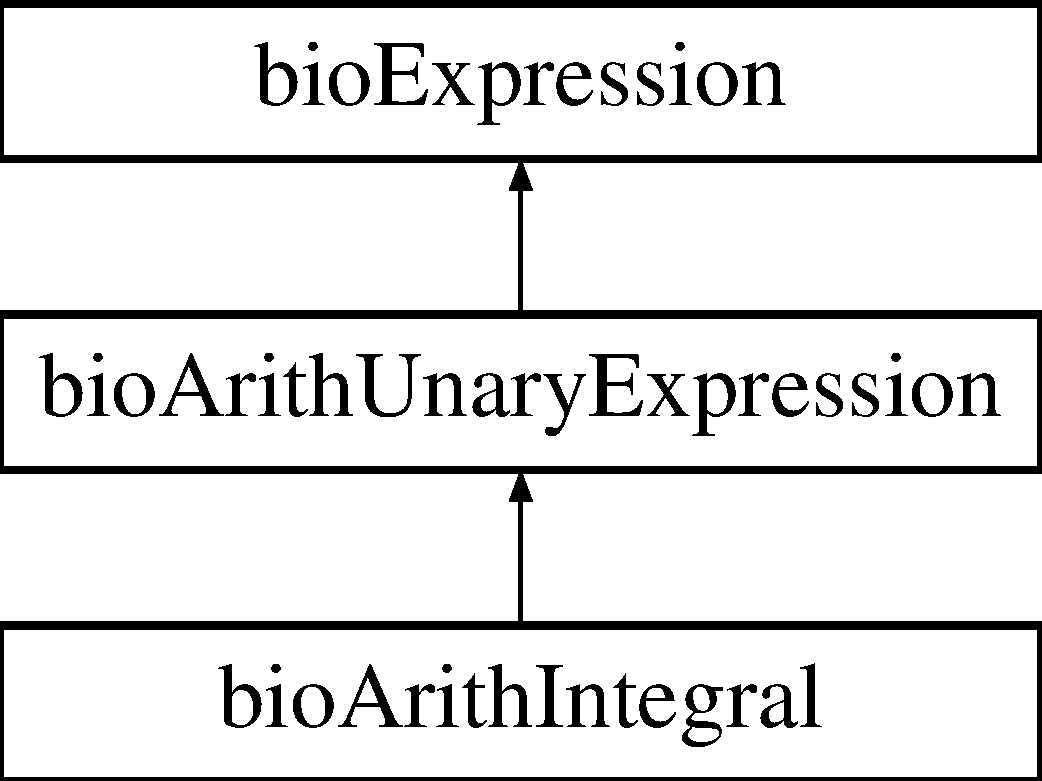
\includegraphics[height=3.000000cm]{classbio_arith_integral}
\end{center}
\end{figure}
\subsection*{Public Member Functions}
\begin{DoxyCompactItemize}
\item 
\mbox{\Hypertarget{classbio_arith_integral_a62142176f2d4ac54ed701082366ad102}\label{classbio_arith_integral_a62142176f2d4ac54ed701082366ad102}} 
{\bfseries bio\+Arith\+Integral} (\hyperlink{classbio_expression_repository}{bio\+Expression\+Repository} $\ast$rep, pat\+U\+Long par, pat\+U\+Long left, pat\+String a\+Literal\+Name, pat\+Error $\ast$\&err)
\item 
virtual pat\+String \hyperlink{classbio_arith_integral_abae8e14e091ddc4e7281ec5ba36f8cf8}{get\+Operator\+Name} () const
\item 
virtual pat\+Real \hyperlink{classbio_arith_integral_a71c94eed284b1ef9e492aa6424c33365}{get\+Value} (pat\+Boolean prepare\+Gradient, pat\+U\+Long current\+Lap, pat\+Error $\ast$\&err)
\item 
virtual \hyperlink{classbio_expression}{bio\+Expression} $\ast$ \hyperlink{classbio_arith_integral_aafdf4edef91568b929fc3e9cd199b202}{get\+Derivative} (pat\+U\+Long a\+Literal\+Id, pat\+Error $\ast$\&err) const
\item 
virtual \hyperlink{classbio_arith_integral}{bio\+Arith\+Integral} $\ast$ \hyperlink{classbio_arith_integral_a49fa38b94818140c143ecb6cb3d7ceed}{get\+Deep\+Copy} (\hyperlink{classbio_expression_repository}{bio\+Expression\+Repository} $\ast$rep, pat\+Error $\ast$\&err) const
\item 
virtual \hyperlink{classbio_arith_integral}{bio\+Arith\+Integral} $\ast$ \hyperlink{classbio_arith_integral_a0a9619e66e582266bf1975d59b7c2bec}{get\+Shallow\+Copy} (\hyperlink{classbio_expression_repository}{bio\+Expression\+Repository} $\ast$rep, pat\+Error $\ast$\&err) const
\item 
virtual pat\+Boolean \hyperlink{classbio_arith_integral_a7f96ce250c987eb2022512c9f65cdc1b}{is\+Structurally\+Zero} () const
\item 
virtual pat\+String \hyperlink{classbio_arith_integral_a597593196620aa13462aebf9166f1678}{get\+Expression\+String} () const
\item 
virtual \hyperlink{classbio_function_and_derivatives}{bio\+Function\+And\+Derivatives} $\ast$ \hyperlink{classbio_arith_integral_a7f9cc73a8a9788b1deb8c2f424606d51}{get\+Numerical\+Function\+And\+Gradient} (vector$<$ pat\+U\+Long $>$ literal\+Ids, pat\+Boolean compute\+Hessian, pat\+Boolean debug\+Derivatives, pat\+Error $\ast$\&err)
\end{DoxyCompactItemize}
\subsection*{Public Attributes}
\begin{DoxyCompactItemize}
\item 
\mbox{\Hypertarget{classbio_arith_integral_adef079988a2f026769bdf7103a40a3d1}\label{classbio_arith_integral_adef079988a2f026769bdf7103a40a3d1}} 
pat\+U\+Long {\bfseries literal\+Id}
\item 
\mbox{\Hypertarget{classbio_arith_integral_ac1fe8365a90bbc1a5dea95236f6712aa}\label{classbio_arith_integral_ac1fe8365a90bbc1a5dea95236f6712aa}} 
pat\+String {\bfseries literal\+Name}
\end{DoxyCompactItemize}
\subsection*{Additional Inherited Members}


\subsection{Detailed Description}
Class implementing a node of the tree representing an integral between -\/infty and +infty 

\subsection{Member Function Documentation}
\mbox{\Hypertarget{classbio_arith_integral_a49fa38b94818140c143ecb6cb3d7ceed}\label{classbio_arith_integral_a49fa38b94818140c143ecb6cb3d7ceed}} 
\index{bio\+Arith\+Integral@{bio\+Arith\+Integral}!get\+Deep\+Copy@{get\+Deep\+Copy}}
\index{get\+Deep\+Copy@{get\+Deep\+Copy}!bio\+Arith\+Integral@{bio\+Arith\+Integral}}
\subsubsection{\texorpdfstring{get\+Deep\+Copy()}{getDeepCopy()}}
{\footnotesize\ttfamily \hyperlink{classbio_arith_integral}{bio\+Arith\+Integral} $\ast$ bio\+Arith\+Integral\+::get\+Deep\+Copy (\begin{DoxyParamCaption}\item[{\hyperlink{classbio_expression_repository}{bio\+Expression\+Repository} $\ast$}]{rep,  }\item[{pat\+Error $\ast$\&}]{err }\end{DoxyParamCaption}) const\hspace{0.3cm}{\ttfamily [virtual]}}

Create a deep copy of the expression and returns a pointer to it. It means that new instances of the children are created. 

Reimplemented from \hyperlink{classbio_expression_a4ee1b8add634078a02eaae26cd40dcc8}{bio\+Expression}.

\mbox{\Hypertarget{classbio_arith_integral_aafdf4edef91568b929fc3e9cd199b202}\label{classbio_arith_integral_aafdf4edef91568b929fc3e9cd199b202}} 
\index{bio\+Arith\+Integral@{bio\+Arith\+Integral}!get\+Derivative@{get\+Derivative}}
\index{get\+Derivative@{get\+Derivative}!bio\+Arith\+Integral@{bio\+Arith\+Integral}}
\subsubsection{\texorpdfstring{get\+Derivative()}{getDerivative()}}
{\footnotesize\ttfamily \hyperlink{classbio_expression}{bio\+Expression} $\ast$ bio\+Arith\+Integral\+::get\+Derivative (\begin{DoxyParamCaption}\item[{pat\+U\+Long}]{a\+Literal\+Id,  }\item[{pat\+Error $\ast$\&}]{err }\end{DoxyParamCaption}) const\hspace{0.3cm}{\ttfamily [virtual]}}

\begin{DoxyReturn}{Returns}
value of the derivative w.\+r.\+t literal 
\end{DoxyReturn}

\begin{DoxyParams}{Parameters}
{\em index} & of the literal involved in the derivative \\
\hline
{\em err} & ref. of the pointer to the error object. \\
\hline
\end{DoxyParams}


Reimplemented from \hyperlink{classbio_expression_a5915579d1193f25f216c1e273c97f2ce}{bio\+Expression}.

\mbox{\Hypertarget{classbio_arith_integral_a597593196620aa13462aebf9166f1678}\label{classbio_arith_integral_a597593196620aa13462aebf9166f1678}} 
\index{bio\+Arith\+Integral@{bio\+Arith\+Integral}!get\+Expression\+String@{get\+Expression\+String}}
\index{get\+Expression\+String@{get\+Expression\+String}!bio\+Arith\+Integral@{bio\+Arith\+Integral}}
\subsubsection{\texorpdfstring{get\+Expression\+String()}{getExpressionString()}}
{\footnotesize\ttfamily pat\+String bio\+Arith\+Integral\+::get\+Expression\+String (\begin{DoxyParamCaption}{ }\end{DoxyParamCaption}) const\hspace{0.3cm}{\ttfamily [virtual]}}

Compute a string that represents the expression. It is designed to replace the expression itself when used only for comparison purposes. Code\+: +\{expr1\}\{expr2\}\+: binary plus -\/\{expr1\}\{expr2\}\+: binary minus \{expr1\}\{expr2\}\+: multiplication /\{expr1\}\{expr2\}\+: division $^\wedge$\{expr1\}\{expr2\}\+: power \&\{expr1\}\{expr2\}\+: and $\vert$\{expr1\}\{expr2\}\+: or =\{expr1\}\{expr2\}\+: equal !=\{expr1\}\{expr2\}\+: not equal $<$\{expr1\}\{expr2\}\+: lesser than $<$=\{expr1\}\{expr2\}\+: lesser or equal to $>$\{expr1\}\{expr2\}\+: greater than $>$=\{expr1\}\{expr2\}\+: greater or equal to \$A\{expr\}\+: abs \$D\mbox{[}expr\mbox{]}\mbox{[}\{expr1\}...\{exprN\}\mbox{]}\+: dictionary (\hyperlink{classbio_arith_elem}{bio\+Arith\+Elem}) \$E\{expr\}\+: exp \$L\{expr\}\+: log \$M\{expr\}\+: Unary minus \$\+Piterator\+\_\+name\{expr\}\+: prod \$Q\{string1\}\{string2\}\+: sequence \$\+Siterator\+\_\+name\{expr\}\+: sum \$\+Ziterator\+\_\+name\mbox{[}\{expr1\}...\{exprN\}\mbox{]}\+: merged sum \{expr1\}\{expr2\}...\{exprN\}//\+: list of expressions number\+: constant \#id\+: literal \&id\+: random 

Reimplemented from \hyperlink{classbio_expression_a3e4b4dca58dbbc6f0e411b30eb3f60b4}{bio\+Expression}.

\mbox{\Hypertarget{classbio_arith_integral_a7f9cc73a8a9788b1deb8c2f424606d51}\label{classbio_arith_integral_a7f9cc73a8a9788b1deb8c2f424606d51}} 
\index{bio\+Arith\+Integral@{bio\+Arith\+Integral}!get\+Numerical\+Function\+And\+Gradient@{get\+Numerical\+Function\+And\+Gradient}}
\index{get\+Numerical\+Function\+And\+Gradient@{get\+Numerical\+Function\+And\+Gradient}!bio\+Arith\+Integral@{bio\+Arith\+Integral}}
\subsubsection{\texorpdfstring{get\+Numerical\+Function\+And\+Gradient()}{getNumericalFunctionAndGradient()}}
{\footnotesize\ttfamily \hyperlink{classbio_function_and_derivatives}{bio\+Function\+And\+Derivatives} $\ast$ bio\+Arith\+Integral\+::get\+Numerical\+Function\+And\+Gradient (\begin{DoxyParamCaption}\item[{vector$<$ pat\+U\+Long $>$}]{literal\+Ids,  }\item[{pat\+Boolean}]{compute\+Hessian,  }\item[{pat\+Boolean}]{debug\+Derivatives,  }\item[{pat\+Error $\ast$\&}]{err }\end{DoxyParamCaption})\hspace{0.3cm}{\ttfamily [virtual]}}

\begin{DoxyReturn}{Returns}
value and gradient of the expression 
\end{DoxyReturn}

\begin{DoxyParams}{Parameters}
{\em err} & ref. of the pointer to the error object. \\
\hline
\end{DoxyParams}


Reimplemented from \hyperlink{classbio_expression_a91c81ce80c9e972c913b10f5f3c1ed13}{bio\+Expression}.

\mbox{\Hypertarget{classbio_arith_integral_abae8e14e091ddc4e7281ec5ba36f8cf8}\label{classbio_arith_integral_abae8e14e091ddc4e7281ec5ba36f8cf8}} 
\index{bio\+Arith\+Integral@{bio\+Arith\+Integral}!get\+Operator\+Name@{get\+Operator\+Name}}
\index{get\+Operator\+Name@{get\+Operator\+Name}!bio\+Arith\+Integral@{bio\+Arith\+Integral}}
\subsubsection{\texorpdfstring{get\+Operator\+Name()}{getOperatorName()}}
{\footnotesize\ttfamily pat\+String bio\+Arith\+Integral\+::get\+Operator\+Name (\begin{DoxyParamCaption}{ }\end{DoxyParamCaption}) const\hspace{0.3cm}{\ttfamily [virtual]}}

\begin{DoxyReturn}{Returns}
name of the operator 
\end{DoxyReturn}


Reimplemented from \hyperlink{classbio_expression_a2353a4afb3a2b0af7c63aba086a72bde}{bio\+Expression}.

\mbox{\Hypertarget{classbio_arith_integral_a0a9619e66e582266bf1975d59b7c2bec}\label{classbio_arith_integral_a0a9619e66e582266bf1975d59b7c2bec}} 
\index{bio\+Arith\+Integral@{bio\+Arith\+Integral}!get\+Shallow\+Copy@{get\+Shallow\+Copy}}
\index{get\+Shallow\+Copy@{get\+Shallow\+Copy}!bio\+Arith\+Integral@{bio\+Arith\+Integral}}
\subsubsection{\texorpdfstring{get\+Shallow\+Copy()}{getShallowCopy()}}
{\footnotesize\ttfamily \hyperlink{classbio_arith_integral}{bio\+Arith\+Integral} $\ast$ bio\+Arith\+Integral\+::get\+Shallow\+Copy (\begin{DoxyParamCaption}\item[{\hyperlink{classbio_expression_repository}{bio\+Expression\+Repository} $\ast$}]{rep,  }\item[{pat\+Error $\ast$\&}]{err }\end{DoxyParamCaption}) const\hspace{0.3cm}{\ttfamily [virtual]}}

Create a shallow copy of the expression and returns a pointer to it. It means that no new instance of the children are created. It is typically called by the repository 

Reimplemented from \hyperlink{classbio_expression_a442534762693b92baaf33928979a1bf8}{bio\+Expression}.

\mbox{\Hypertarget{classbio_arith_integral_a71c94eed284b1ef9e492aa6424c33365}\label{classbio_arith_integral_a71c94eed284b1ef9e492aa6424c33365}} 
\index{bio\+Arith\+Integral@{bio\+Arith\+Integral}!get\+Value@{get\+Value}}
\index{get\+Value@{get\+Value}!bio\+Arith\+Integral@{bio\+Arith\+Integral}}
\subsubsection{\texorpdfstring{get\+Value()}{getValue()}}
{\footnotesize\ttfamily pat\+Real bio\+Arith\+Integral\+::get\+Value (\begin{DoxyParamCaption}\item[{pat\+Boolean}]{prepare\+Gradient,  }\item[{pat\+U\+Long}]{current\+Lap,  }\item[{pat\+Error $\ast$\&}]{err }\end{DoxyParamCaption})\hspace{0.3cm}{\ttfamily [virtual]}}

\begin{DoxyReturn}{Returns}
value of the expression 
\end{DoxyReturn}

\begin{DoxyParams}{Parameters}
{\em err} & ref. of the pointer to the error object. \\
\hline
\end{DoxyParams}


Reimplemented from \hyperlink{classbio_expression_af58662a5d4d456f15bc4f2c9bd4f8a5b}{bio\+Expression}.

\mbox{\Hypertarget{classbio_arith_integral_a7f96ce250c987eb2022512c9f65cdc1b}\label{classbio_arith_integral_a7f96ce250c987eb2022512c9f65cdc1b}} 
\index{bio\+Arith\+Integral@{bio\+Arith\+Integral}!is\+Structurally\+Zero@{is\+Structurally\+Zero}}
\index{is\+Structurally\+Zero@{is\+Structurally\+Zero}!bio\+Arith\+Integral@{bio\+Arith\+Integral}}
\subsubsection{\texorpdfstring{is\+Structurally\+Zero()}{isStructurallyZero()}}
{\footnotesize\ttfamily pat\+Boolean bio\+Arith\+Integral\+::is\+Structurally\+Zero (\begin{DoxyParamCaption}{ }\end{DoxyParamCaption}) const\hspace{0.3cm}{\ttfamily [virtual]}}

return pat\+T\+R\+UE if the expression is structurally 0 so that there is no need to evaluate it. In the base class, it return pat\+F\+A\+L\+SE. 

Reimplemented from \hyperlink{classbio_expression_a264c6d78671610ada8261d698e4c4c42}{bio\+Expression}.



The documentation for this class was generated from the following files\+:\begin{DoxyCompactItemize}
\item 
bio\+Arith\+Integral.\+h\item 
bio\+Arith\+Integral.\+cc\end{DoxyCompactItemize}

\hypertarget{classbio_arith_iterator}{}\section{bio\+Arith\+Iterator Class Reference}
\label{classbio_arith_iterator}\index{bio\+Arith\+Iterator@{bio\+Arith\+Iterator}}


{\ttfamily \#include $<$bio\+Arith\+Iterator.\+h$>$}

Inheritance diagram for bio\+Arith\+Iterator\+:\begin{figure}[H]
\begin{center}
\leavevmode
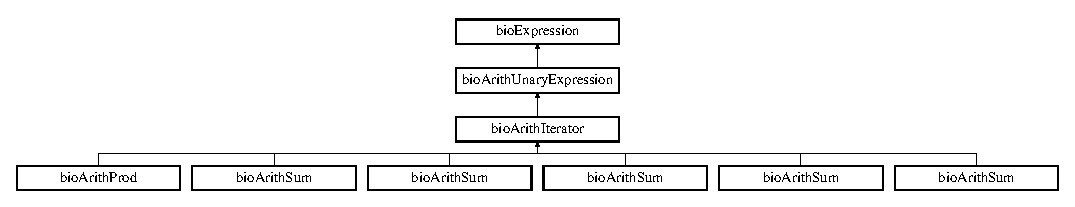
\includegraphics[height=2.333333cm]{classbio_arith_iterator}
\end{center}
\end{figure}
\subsection*{Public Member Functions}
\begin{DoxyCompactItemize}
\item 
\mbox{\Hypertarget{classbio_arith_iterator_aa462a3be033addf63a71f4dc2587ce69}\label{classbio_arith_iterator_aa462a3be033addf63a71f4dc2587ce69}} 
{\bfseries bio\+Arith\+Iterator} (\hyperlink{classbio_expression_repository}{bio\+Expression\+Repository} $\ast$rep, pat\+U\+Long par, pat\+U\+Long left, pat\+String an\+Iterator, pat\+Error $\ast$\&err)
\item 
virtual pat\+String \hyperlink{classbio_arith_iterator_aceb6ee1a4c024349178de5edf4624710}{get\+Expression} (pat\+Error $\ast$\&err) const
\item 
virtual pat\+String \hyperlink{classbio_arith_iterator_a0e3f7a50861a44e7a62216e5a192a838}{the\+Iterator} () const
\item 
\mbox{\Hypertarget{classbio_arith_iterator_ad3333ec910f68aa3c658502dc61f8c44}\label{classbio_arith_iterator_ad3333ec910f68aa3c658502dc61f8c44}} 
virtual pat\+Boolean {\bfseries is\+Sum} () const
\item 
\mbox{\Hypertarget{classbio_arith_iterator_a0110ce3c484d5a61d314ea5a8c51618f}\label{classbio_arith_iterator_a0110ce3c484d5a61d314ea5a8c51618f}} 
virtual pat\+Boolean {\bfseries is\+Prod} () const
\item 
\mbox{\Hypertarget{classbio_arith_iterator_ab99e052d4167e099c6469278d8f3fe77}\label{classbio_arith_iterator_ab99e052d4167e099c6469278d8f3fe77}} 
virtual pat\+Boolean {\bfseries contains\+An\+Iterator} () const
\item 
\mbox{\Hypertarget{classbio_arith_iterator_acf59ada258bca97acb1624942a06e5e0}\label{classbio_arith_iterator_acf59ada258bca97acb1624942a06e5e0}} 
virtual pat\+Boolean {\bfseries contains\+An\+Iterator\+On\+Rows} () const
\end{DoxyCompactItemize}
\subsection*{Protected Attributes}
\begin{DoxyCompactItemize}
\item 
\mbox{\Hypertarget{classbio_arith_iterator_a44e87dc91e2382f8ab09346eb1be8cb0}\label{classbio_arith_iterator_a44e87dc91e2382f8ab09346eb1be8cb0}} 
pat\+String {\bfseries the\+Iterator\+Name}
\item 
\mbox{\Hypertarget{classbio_arith_iterator_a0338b170a0f40968c6f7e4f23231bf40}\label{classbio_arith_iterator_a0338b170a0f40968c6f7e4f23231bf40}} 
bio\+Iterator\+Type {\bfseries the\+Iterator\+Type}
\end{DoxyCompactItemize}


\subsection{Detailed Description}
Class implementing a node of the tree representing a sum or a prod expression 

\subsection{Member Function Documentation}
\mbox{\Hypertarget{classbio_arith_iterator_aceb6ee1a4c024349178de5edf4624710}\label{classbio_arith_iterator_aceb6ee1a4c024349178de5edf4624710}} 
\index{bio\+Arith\+Iterator@{bio\+Arith\+Iterator}!get\+Expression@{get\+Expression}}
\index{get\+Expression@{get\+Expression}!bio\+Arith\+Iterator@{bio\+Arith\+Iterator}}
\subsubsection{\texorpdfstring{get\+Expression()}{getExpression()}}
{\footnotesize\ttfamily pat\+String bio\+Arith\+Iterator\+::get\+Expression (\begin{DoxyParamCaption}\item[{pat\+Error $\ast$\&}]{err }\end{DoxyParamCaption}) const\hspace{0.3cm}{\ttfamily [virtual]}}

\begin{DoxyReturn}{Returns}
printed expression 
\end{DoxyReturn}


Reimplemented from \hyperlink{classbio_arith_unary_expression_a974b7779804861f331a75e08db377926}{bio\+Arith\+Unary\+Expression}.

\mbox{\Hypertarget{classbio_arith_iterator_a0e3f7a50861a44e7a62216e5a192a838}\label{classbio_arith_iterator_a0e3f7a50861a44e7a62216e5a192a838}} 
\index{bio\+Arith\+Iterator@{bio\+Arith\+Iterator}!the\+Iterator@{the\+Iterator}}
\index{the\+Iterator@{the\+Iterator}!bio\+Arith\+Iterator@{bio\+Arith\+Iterator}}
\subsubsection{\texorpdfstring{the\+Iterator()}{theIterator()}}
{\footnotesize\ttfamily pat\+String bio\+Arith\+Iterator\+::the\+Iterator (\begin{DoxyParamCaption}{ }\end{DoxyParamCaption}) const\hspace{0.3cm}{\ttfamily [virtual]}}

\begin{DoxyReturn}{Returns}
pointer to the iterator information if the top level node is an iterator, N\+U\+LL otherwise. Not recursive. 
\end{DoxyReturn}


Reimplemented from \hyperlink{classbio_expression_a9830c0cf012012c811b826adc54291f6}{bio\+Expression}.



The documentation for this class was generated from the following files\+:\begin{DoxyCompactItemize}
\item 
bio\+Arith\+Iterator.\+h\item 
bio\+Arith\+Iterator.\+cc\end{DoxyCompactItemize}

\hypertarget{classbio_arith_less}{}\section{bio\+Arith\+Less Class Reference}
\label{classbio_arith_less}\index{bio\+Arith\+Less@{bio\+Arith\+Less}}


{\ttfamily \#include $<$bio\+Arith\+Less.\+h$>$}

Inheritance diagram for bio\+Arith\+Less\+:\begin{figure}[H]
\begin{center}
\leavevmode
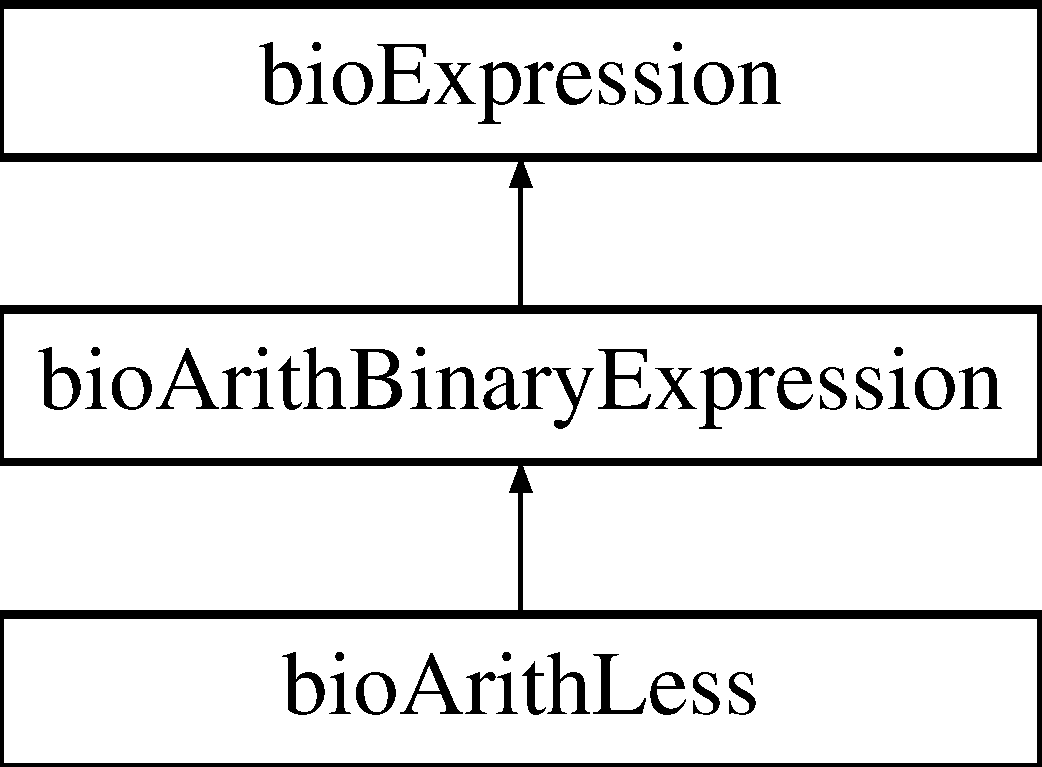
\includegraphics[height=3.000000cm]{classbio_arith_less}
\end{center}
\end{figure}
\subsection*{Public Member Functions}
\begin{DoxyCompactItemize}
\item 
\mbox{\Hypertarget{classbio_arith_less_a94229f67cdd192ea9524c94f51bbecb7}\label{classbio_arith_less_a94229f67cdd192ea9524c94f51bbecb7}} 
{\bfseries bio\+Arith\+Less} (\hyperlink{classbio_expression_repository}{bio\+Expression\+Repository} $\ast$rep, pat\+U\+Long par, pat\+U\+Long left, pat\+U\+Long right, pat\+Error $\ast$\&err)
\item 
virtual pat\+String \hyperlink{classbio_arith_less_a0be270c31ac0cec7d6e23dfe9558a138}{get\+Operator\+Name} () const
\item 
virtual pat\+Real \hyperlink{classbio_arith_less_aa53cd0dfe26ec7e75b760661b940ac0d}{get\+Value} (pat\+Boolean prepare\+Gradient, pat\+U\+Long current\+Lap, pat\+Error $\ast$\&err)
\item 
virtual \hyperlink{classbio_expression}{bio\+Expression} $\ast$ \hyperlink{classbio_arith_less_a031bd542ab09a456fcdd4f4e121d2940}{get\+Derivative} (pat\+U\+Long a\+Literal\+Id, pat\+Error $\ast$\&err) const
\item 
virtual \hyperlink{classbio_arith_less}{bio\+Arith\+Less} $\ast$ \hyperlink{classbio_arith_less_a44f8cd0243ba7997d9799537c099c5a8}{get\+Deep\+Copy} (\hyperlink{classbio_expression_repository}{bio\+Expression\+Repository} $\ast$rep, pat\+Error $\ast$\&err) const
\item 
virtual \hyperlink{classbio_arith_less}{bio\+Arith\+Less} $\ast$ \hyperlink{classbio_arith_less_a186b89363273b2972ae1beb00a1efbb0}{get\+Shallow\+Copy} (\hyperlink{classbio_expression_repository}{bio\+Expression\+Repository} $\ast$rep, pat\+Error $\ast$\&err) const
\item 
virtual pat\+String \hyperlink{classbio_arith_less_a8f9d063a00ed8a65ea2b37e3d63405f8}{get\+Expression\+String} () const
\item 
virtual \hyperlink{classbio_function_and_derivatives}{bio\+Function\+And\+Derivatives} $\ast$ \hyperlink{classbio_arith_less_a03309258107a65a08f59b00878eec548}{get\+Numerical\+Function\+And\+Gradient} (vector$<$ pat\+U\+Long $>$ literal\+Ids, pat\+Boolean compute\+Hessian, pat\+Boolean debug\+Derivatives, pat\+Error $\ast$\&err)
\end{DoxyCompactItemize}
\subsection*{Additional Inherited Members}


\subsection{Detailed Description}
Class implementing a node of the tree representing a comparison ($<$) operation 

\subsection{Member Function Documentation}
\mbox{\Hypertarget{classbio_arith_less_a44f8cd0243ba7997d9799537c099c5a8}\label{classbio_arith_less_a44f8cd0243ba7997d9799537c099c5a8}} 
\index{bio\+Arith\+Less@{bio\+Arith\+Less}!get\+Deep\+Copy@{get\+Deep\+Copy}}
\index{get\+Deep\+Copy@{get\+Deep\+Copy}!bio\+Arith\+Less@{bio\+Arith\+Less}}
\subsubsection{\texorpdfstring{get\+Deep\+Copy()}{getDeepCopy()}}
{\footnotesize\ttfamily \hyperlink{classbio_arith_less}{bio\+Arith\+Less} $\ast$ bio\+Arith\+Less\+::get\+Deep\+Copy (\begin{DoxyParamCaption}\item[{\hyperlink{classbio_expression_repository}{bio\+Expression\+Repository} $\ast$}]{rep,  }\item[{pat\+Error $\ast$\&}]{err }\end{DoxyParamCaption}) const\hspace{0.3cm}{\ttfamily [virtual]}}

Create a deep copy of the expression and returns a pointer to it. It means that new instances of the children are created. 

Reimplemented from \hyperlink{classbio_expression_a4ee1b8add634078a02eaae26cd40dcc8}{bio\+Expression}.

\mbox{\Hypertarget{classbio_arith_less_a031bd542ab09a456fcdd4f4e121d2940}\label{classbio_arith_less_a031bd542ab09a456fcdd4f4e121d2940}} 
\index{bio\+Arith\+Less@{bio\+Arith\+Less}!get\+Derivative@{get\+Derivative}}
\index{get\+Derivative@{get\+Derivative}!bio\+Arith\+Less@{bio\+Arith\+Less}}
\subsubsection{\texorpdfstring{get\+Derivative()}{getDerivative()}}
{\footnotesize\ttfamily \hyperlink{classbio_expression}{bio\+Expression} $\ast$ bio\+Arith\+Less\+::get\+Derivative (\begin{DoxyParamCaption}\item[{pat\+U\+Long}]{a\+Literal\+Id,  }\item[{pat\+Error $\ast$\&}]{err }\end{DoxyParamCaption}) const\hspace{0.3cm}{\ttfamily [virtual]}}

\begin{DoxyReturn}{Returns}
value of the derivative w.\+r.\+t literal 
\end{DoxyReturn}

\begin{DoxyParams}{Parameters}
{\em index} & of the literal involved in the derivative \\
\hline
{\em err} & ref. of the pointer to the error object. \\
\hline
\end{DoxyParams}


Reimplemented from \hyperlink{classbio_expression_a5915579d1193f25f216c1e273c97f2ce}{bio\+Expression}.

\mbox{\Hypertarget{classbio_arith_less_a8f9d063a00ed8a65ea2b37e3d63405f8}\label{classbio_arith_less_a8f9d063a00ed8a65ea2b37e3d63405f8}} 
\index{bio\+Arith\+Less@{bio\+Arith\+Less}!get\+Expression\+String@{get\+Expression\+String}}
\index{get\+Expression\+String@{get\+Expression\+String}!bio\+Arith\+Less@{bio\+Arith\+Less}}
\subsubsection{\texorpdfstring{get\+Expression\+String()}{getExpressionString()}}
{\footnotesize\ttfamily pat\+String bio\+Arith\+Less\+::get\+Expression\+String (\begin{DoxyParamCaption}{ }\end{DoxyParamCaption}) const\hspace{0.3cm}{\ttfamily [virtual]}}

Compute a string that represents the expression. It is designed to replace the expression itself when used only for comparison purposes. Code\+: +\{expr1\}\{expr2\}\+: binary plus -\/\{expr1\}\{expr2\}\+: binary minus \{expr1\}\{expr2\}\+: multiplication /\{expr1\}\{expr2\}\+: division $^\wedge$\{expr1\}\{expr2\}\+: power \&\{expr1\}\{expr2\}\+: and $\vert$\{expr1\}\{expr2\}\+: or =\{expr1\}\{expr2\}\+: equal !=\{expr1\}\{expr2\}\+: not equal $<$\{expr1\}\{expr2\}\+: lesser than $<$=\{expr1\}\{expr2\}\+: lesser or equal to $>$\{expr1\}\{expr2\}\+: greater than $>$=\{expr1\}\{expr2\}\+: greater or equal to \$A\{expr\}\+: abs \$D\mbox{[}expr\mbox{]}\mbox{[}\{expr1\}...\{exprN\}\mbox{]}\+: dictionary (\hyperlink{classbio_arith_elem}{bio\+Arith\+Elem}) \$E\{expr\}\+: exp \$L\{expr\}\+: log \$M\{expr\}\+: Unary minus \$\+Piterator\+\_\+name\{expr\}\+: prod \$Q\{string1\}\{string2\}\+: sequence \$\+Siterator\+\_\+name\{expr\}\+: sum \$\+Ziterator\+\_\+name\mbox{[}\{expr1\}...\{exprN\}\mbox{]}\+: merged sum \{expr1\}\{expr2\}...\{exprN\}//\+: list of expressions number\+: constant \#id\+: literal \&id\+: random 

Reimplemented from \hyperlink{classbio_expression_a3e4b4dca58dbbc6f0e411b30eb3f60b4}{bio\+Expression}.

\mbox{\Hypertarget{classbio_arith_less_a03309258107a65a08f59b00878eec548}\label{classbio_arith_less_a03309258107a65a08f59b00878eec548}} 
\index{bio\+Arith\+Less@{bio\+Arith\+Less}!get\+Numerical\+Function\+And\+Gradient@{get\+Numerical\+Function\+And\+Gradient}}
\index{get\+Numerical\+Function\+And\+Gradient@{get\+Numerical\+Function\+And\+Gradient}!bio\+Arith\+Less@{bio\+Arith\+Less}}
\subsubsection{\texorpdfstring{get\+Numerical\+Function\+And\+Gradient()}{getNumericalFunctionAndGradient()}}
{\footnotesize\ttfamily \hyperlink{classbio_function_and_derivatives}{bio\+Function\+And\+Derivatives} $\ast$ bio\+Arith\+Less\+::get\+Numerical\+Function\+And\+Gradient (\begin{DoxyParamCaption}\item[{vector$<$ pat\+U\+Long $>$}]{literal\+Ids,  }\item[{pat\+Boolean}]{compute\+Hessian,  }\item[{pat\+Boolean}]{debug\+Derivatives,  }\item[{pat\+Error $\ast$\&}]{err }\end{DoxyParamCaption})\hspace{0.3cm}{\ttfamily [virtual]}}

\begin{DoxyReturn}{Returns}
value and gradient of the expression 
\end{DoxyReturn}

\begin{DoxyParams}{Parameters}
{\em err} & ref. of the pointer to the error object. \\
\hline
\end{DoxyParams}


Reimplemented from \hyperlink{classbio_expression_a91c81ce80c9e972c913b10f5f3c1ed13}{bio\+Expression}.

\mbox{\Hypertarget{classbio_arith_less_a0be270c31ac0cec7d6e23dfe9558a138}\label{classbio_arith_less_a0be270c31ac0cec7d6e23dfe9558a138}} 
\index{bio\+Arith\+Less@{bio\+Arith\+Less}!get\+Operator\+Name@{get\+Operator\+Name}}
\index{get\+Operator\+Name@{get\+Operator\+Name}!bio\+Arith\+Less@{bio\+Arith\+Less}}
\subsubsection{\texorpdfstring{get\+Operator\+Name()}{getOperatorName()}}
{\footnotesize\ttfamily pat\+String bio\+Arith\+Less\+::get\+Operator\+Name (\begin{DoxyParamCaption}{ }\end{DoxyParamCaption}) const\hspace{0.3cm}{\ttfamily [virtual]}}

\begin{DoxyReturn}{Returns}
name of the operator 
\end{DoxyReturn}


Reimplemented from \hyperlink{classbio_expression_a2353a4afb3a2b0af7c63aba086a72bde}{bio\+Expression}.

\mbox{\Hypertarget{classbio_arith_less_a186b89363273b2972ae1beb00a1efbb0}\label{classbio_arith_less_a186b89363273b2972ae1beb00a1efbb0}} 
\index{bio\+Arith\+Less@{bio\+Arith\+Less}!get\+Shallow\+Copy@{get\+Shallow\+Copy}}
\index{get\+Shallow\+Copy@{get\+Shallow\+Copy}!bio\+Arith\+Less@{bio\+Arith\+Less}}
\subsubsection{\texorpdfstring{get\+Shallow\+Copy()}{getShallowCopy()}}
{\footnotesize\ttfamily \hyperlink{classbio_arith_less}{bio\+Arith\+Less} $\ast$ bio\+Arith\+Less\+::get\+Shallow\+Copy (\begin{DoxyParamCaption}\item[{\hyperlink{classbio_expression_repository}{bio\+Expression\+Repository} $\ast$}]{rep,  }\item[{pat\+Error $\ast$\&}]{err }\end{DoxyParamCaption}) const\hspace{0.3cm}{\ttfamily [virtual]}}

Create a shallow copy of the expression and returns a pointer to it. It means that no new instance of the children are created. It is typically called by the repository 

Reimplemented from \hyperlink{classbio_expression_a442534762693b92baaf33928979a1bf8}{bio\+Expression}.

\mbox{\Hypertarget{classbio_arith_less_aa53cd0dfe26ec7e75b760661b940ac0d}\label{classbio_arith_less_aa53cd0dfe26ec7e75b760661b940ac0d}} 
\index{bio\+Arith\+Less@{bio\+Arith\+Less}!get\+Value@{get\+Value}}
\index{get\+Value@{get\+Value}!bio\+Arith\+Less@{bio\+Arith\+Less}}
\subsubsection{\texorpdfstring{get\+Value()}{getValue()}}
{\footnotesize\ttfamily pat\+Real bio\+Arith\+Less\+::get\+Value (\begin{DoxyParamCaption}\item[{pat\+Boolean}]{prepare\+Gradient,  }\item[{pat\+U\+Long}]{current\+Lap,  }\item[{pat\+Error $\ast$\&}]{err }\end{DoxyParamCaption})\hspace{0.3cm}{\ttfamily [virtual]}}

\begin{DoxyReturn}{Returns}
value of the expression 
\end{DoxyReturn}

\begin{DoxyParams}{Parameters}
{\em err} & ref. of the pointer to the error object. \\
\hline
\end{DoxyParams}


Reimplemented from \hyperlink{classbio_expression_af58662a5d4d456f15bc4f2c9bd4f8a5b}{bio\+Expression}.



The documentation for this class was generated from the following files\+:\begin{DoxyCompactItemize}
\item 
bio\+Arith\+Less.\+h\item 
bio\+Arith\+Less.\+cc\end{DoxyCompactItemize}

\hypertarget{classbio_arith_less_equal}{}\section{bio\+Arith\+Less\+Equal Class Reference}
\label{classbio_arith_less_equal}\index{bio\+Arith\+Less\+Equal@{bio\+Arith\+Less\+Equal}}


{\ttfamily \#include $<$bio\+Arith\+Less\+Equal.\+h$>$}

Inheritance diagram for bio\+Arith\+Less\+Equal\+:\begin{figure}[H]
\begin{center}
\leavevmode
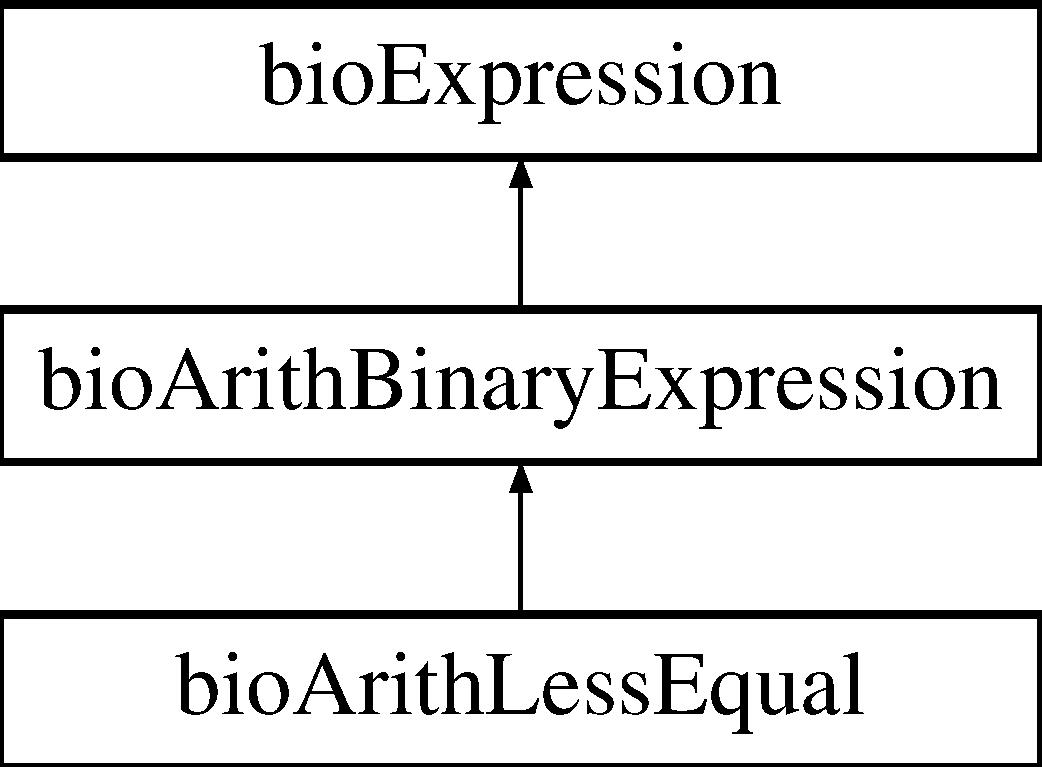
\includegraphics[height=3.000000cm]{classbio_arith_less_equal}
\end{center}
\end{figure}
\subsection*{Public Member Functions}
\begin{DoxyCompactItemize}
\item 
\mbox{\Hypertarget{classbio_arith_less_equal_ab139689812ae96fca0155df7ec67f189}\label{classbio_arith_less_equal_ab139689812ae96fca0155df7ec67f189}} 
{\bfseries bio\+Arith\+Less\+Equal} (\hyperlink{classbio_expression_repository}{bio\+Expression\+Repository} $\ast$rep, pat\+U\+Long par, pat\+U\+Long left, pat\+U\+Long right, pat\+Error $\ast$\&err)
\item 
virtual pat\+String \hyperlink{classbio_arith_less_equal_ad33162b75241a2efee3ace47e899de11}{get\+Operator\+Name} () const
\item 
virtual pat\+Real \hyperlink{classbio_arith_less_equal_af1741ef7a088b6a961889cd82fae3206}{get\+Value} (pat\+Boolean prepare\+Gradient, pat\+U\+Long current\+Lap, pat\+Error $\ast$\&err)
\item 
virtual \hyperlink{classbio_expression}{bio\+Expression} $\ast$ \hyperlink{classbio_arith_less_equal_aaaa08c34c10d1b89378dd0c67917239b}{get\+Derivative} (pat\+U\+Long a\+Literal\+Id, pat\+Error $\ast$\&err) const
\item 
virtual \hyperlink{classbio_arith_less_equal}{bio\+Arith\+Less\+Equal} $\ast$ \hyperlink{classbio_arith_less_equal_a47bbe003d35d47d8ff6545a5cf8dd389}{get\+Deep\+Copy} (\hyperlink{classbio_expression_repository}{bio\+Expression\+Repository} $\ast$rep, pat\+Error $\ast$\&err) const
\item 
virtual \hyperlink{classbio_arith_less_equal}{bio\+Arith\+Less\+Equal} $\ast$ \hyperlink{classbio_arith_less_equal_a47164bfceb3759082555502a38e9f70b}{get\+Shallow\+Copy} (\hyperlink{classbio_expression_repository}{bio\+Expression\+Repository} $\ast$rep, pat\+Error $\ast$\&err) const
\item 
virtual pat\+String \hyperlink{classbio_arith_less_equal_a82a5b4eeb77747bc674fbc16453f9d67}{get\+Expression\+String} () const
\item 
virtual \hyperlink{classbio_function_and_derivatives}{bio\+Function\+And\+Derivatives} $\ast$ \hyperlink{classbio_arith_less_equal_a718044c38d59fc7639656a7754bfb090}{get\+Numerical\+Function\+And\+Gradient} (vector$<$ pat\+U\+Long $>$ literal\+Ids, pat\+Boolean compute\+Hessian, pat\+Boolean debug\+Derivatives, pat\+Error $\ast$\&err)
\end{DoxyCompactItemize}
\subsection*{Additional Inherited Members}


\subsection{Detailed Description}
Class implementing a node of the tree representing a comparison ($<$=) operation 

\subsection{Member Function Documentation}
\mbox{\Hypertarget{classbio_arith_less_equal_a47bbe003d35d47d8ff6545a5cf8dd389}\label{classbio_arith_less_equal_a47bbe003d35d47d8ff6545a5cf8dd389}} 
\index{bio\+Arith\+Less\+Equal@{bio\+Arith\+Less\+Equal}!get\+Deep\+Copy@{get\+Deep\+Copy}}
\index{get\+Deep\+Copy@{get\+Deep\+Copy}!bio\+Arith\+Less\+Equal@{bio\+Arith\+Less\+Equal}}
\subsubsection{\texorpdfstring{get\+Deep\+Copy()}{getDeepCopy()}}
{\footnotesize\ttfamily \hyperlink{classbio_arith_less_equal}{bio\+Arith\+Less\+Equal} $\ast$ bio\+Arith\+Less\+Equal\+::get\+Deep\+Copy (\begin{DoxyParamCaption}\item[{\hyperlink{classbio_expression_repository}{bio\+Expression\+Repository} $\ast$}]{rep,  }\item[{pat\+Error $\ast$\&}]{err }\end{DoxyParamCaption}) const\hspace{0.3cm}{\ttfamily [virtual]}}

Create a deep copy of the expression and returns a pointer to it. It means that new instances of the children are created. 

Reimplemented from \hyperlink{classbio_expression_a4ee1b8add634078a02eaae26cd40dcc8}{bio\+Expression}.

\mbox{\Hypertarget{classbio_arith_less_equal_aaaa08c34c10d1b89378dd0c67917239b}\label{classbio_arith_less_equal_aaaa08c34c10d1b89378dd0c67917239b}} 
\index{bio\+Arith\+Less\+Equal@{bio\+Arith\+Less\+Equal}!get\+Derivative@{get\+Derivative}}
\index{get\+Derivative@{get\+Derivative}!bio\+Arith\+Less\+Equal@{bio\+Arith\+Less\+Equal}}
\subsubsection{\texorpdfstring{get\+Derivative()}{getDerivative()}}
{\footnotesize\ttfamily \hyperlink{classbio_expression}{bio\+Expression} $\ast$ bio\+Arith\+Less\+Equal\+::get\+Derivative (\begin{DoxyParamCaption}\item[{pat\+U\+Long}]{a\+Literal\+Id,  }\item[{pat\+Error $\ast$\&}]{err }\end{DoxyParamCaption}) const\hspace{0.3cm}{\ttfamily [virtual]}}

\begin{DoxyReturn}{Returns}
value of the derivative w.\+r.\+t literal 
\end{DoxyReturn}

\begin{DoxyParams}{Parameters}
{\em index} & of the literal involved in the derivative \\
\hline
{\em err} & ref. of the pointer to the error object. \\
\hline
\end{DoxyParams}


Reimplemented from \hyperlink{classbio_expression_a5915579d1193f25f216c1e273c97f2ce}{bio\+Expression}.

\mbox{\Hypertarget{classbio_arith_less_equal_a82a5b4eeb77747bc674fbc16453f9d67}\label{classbio_arith_less_equal_a82a5b4eeb77747bc674fbc16453f9d67}} 
\index{bio\+Arith\+Less\+Equal@{bio\+Arith\+Less\+Equal}!get\+Expression\+String@{get\+Expression\+String}}
\index{get\+Expression\+String@{get\+Expression\+String}!bio\+Arith\+Less\+Equal@{bio\+Arith\+Less\+Equal}}
\subsubsection{\texorpdfstring{get\+Expression\+String()}{getExpressionString()}}
{\footnotesize\ttfamily pat\+String bio\+Arith\+Less\+Equal\+::get\+Expression\+String (\begin{DoxyParamCaption}{ }\end{DoxyParamCaption}) const\hspace{0.3cm}{\ttfamily [virtual]}}

Compute a string that represents the expression. It is designed to replace the expression itself when used only for comparison purposes. Code\+: +\{expr1\}\{expr2\}\+: binary plus -\/\{expr1\}\{expr2\}\+: binary minus \{expr1\}\{expr2\}\+: multiplication /\{expr1\}\{expr2\}\+: division $^\wedge$\{expr1\}\{expr2\}\+: power \&\{expr1\}\{expr2\}\+: and $\vert$\{expr1\}\{expr2\}\+: or =\{expr1\}\{expr2\}\+: equal !=\{expr1\}\{expr2\}\+: not equal $<$\{expr1\}\{expr2\}\+: lesser than $<$=\{expr1\}\{expr2\}\+: lesser or equal to $>$\{expr1\}\{expr2\}\+: greater than $>$=\{expr1\}\{expr2\}\+: greater or equal to \$A\{expr\}\+: abs \$D\mbox{[}expr\mbox{]}\mbox{[}\{expr1\}...\{exprN\}\mbox{]}\+: dictionary (\hyperlink{classbio_arith_elem}{bio\+Arith\+Elem}) \$E\{expr\}\+: exp \$L\{expr\}\+: log \$M\{expr\}\+: Unary minus \$\+Piterator\+\_\+name\{expr\}\+: prod \$Q\{string1\}\{string2\}\+: sequence \$\+Siterator\+\_\+name\{expr\}\+: sum \$\+Ziterator\+\_\+name\mbox{[}\{expr1\}...\{exprN\}\mbox{]}\+: merged sum \{expr1\}\{expr2\}...\{exprN\}//\+: list of expressions number\+: constant \#id\+: literal \&id\+: random 

Reimplemented from \hyperlink{classbio_expression_a3e4b4dca58dbbc6f0e411b30eb3f60b4}{bio\+Expression}.

\mbox{\Hypertarget{classbio_arith_less_equal_a718044c38d59fc7639656a7754bfb090}\label{classbio_arith_less_equal_a718044c38d59fc7639656a7754bfb090}} 
\index{bio\+Arith\+Less\+Equal@{bio\+Arith\+Less\+Equal}!get\+Numerical\+Function\+And\+Gradient@{get\+Numerical\+Function\+And\+Gradient}}
\index{get\+Numerical\+Function\+And\+Gradient@{get\+Numerical\+Function\+And\+Gradient}!bio\+Arith\+Less\+Equal@{bio\+Arith\+Less\+Equal}}
\subsubsection{\texorpdfstring{get\+Numerical\+Function\+And\+Gradient()}{getNumericalFunctionAndGradient()}}
{\footnotesize\ttfamily \hyperlink{classbio_function_and_derivatives}{bio\+Function\+And\+Derivatives} $\ast$ bio\+Arith\+Less\+Equal\+::get\+Numerical\+Function\+And\+Gradient (\begin{DoxyParamCaption}\item[{vector$<$ pat\+U\+Long $>$}]{literal\+Ids,  }\item[{pat\+Boolean}]{compute\+Hessian,  }\item[{pat\+Boolean}]{debug\+Derivatives,  }\item[{pat\+Error $\ast$\&}]{err }\end{DoxyParamCaption})\hspace{0.3cm}{\ttfamily [virtual]}}

\begin{DoxyReturn}{Returns}
value and gradient of the expression 
\end{DoxyReturn}

\begin{DoxyParams}{Parameters}
{\em err} & ref. of the pointer to the error object. \\
\hline
\end{DoxyParams}


Reimplemented from \hyperlink{classbio_expression_a91c81ce80c9e972c913b10f5f3c1ed13}{bio\+Expression}.

\mbox{\Hypertarget{classbio_arith_less_equal_ad33162b75241a2efee3ace47e899de11}\label{classbio_arith_less_equal_ad33162b75241a2efee3ace47e899de11}} 
\index{bio\+Arith\+Less\+Equal@{bio\+Arith\+Less\+Equal}!get\+Operator\+Name@{get\+Operator\+Name}}
\index{get\+Operator\+Name@{get\+Operator\+Name}!bio\+Arith\+Less\+Equal@{bio\+Arith\+Less\+Equal}}
\subsubsection{\texorpdfstring{get\+Operator\+Name()}{getOperatorName()}}
{\footnotesize\ttfamily pat\+String bio\+Arith\+Less\+Equal\+::get\+Operator\+Name (\begin{DoxyParamCaption}{ }\end{DoxyParamCaption}) const\hspace{0.3cm}{\ttfamily [virtual]}}

\begin{DoxyReturn}{Returns}
name of the operator 
\end{DoxyReturn}


Reimplemented from \hyperlink{classbio_expression_a2353a4afb3a2b0af7c63aba086a72bde}{bio\+Expression}.

\mbox{\Hypertarget{classbio_arith_less_equal_a47164bfceb3759082555502a38e9f70b}\label{classbio_arith_less_equal_a47164bfceb3759082555502a38e9f70b}} 
\index{bio\+Arith\+Less\+Equal@{bio\+Arith\+Less\+Equal}!get\+Shallow\+Copy@{get\+Shallow\+Copy}}
\index{get\+Shallow\+Copy@{get\+Shallow\+Copy}!bio\+Arith\+Less\+Equal@{bio\+Arith\+Less\+Equal}}
\subsubsection{\texorpdfstring{get\+Shallow\+Copy()}{getShallowCopy()}}
{\footnotesize\ttfamily \hyperlink{classbio_arith_less_equal}{bio\+Arith\+Less\+Equal} $\ast$ bio\+Arith\+Less\+Equal\+::get\+Shallow\+Copy (\begin{DoxyParamCaption}\item[{\hyperlink{classbio_expression_repository}{bio\+Expression\+Repository} $\ast$}]{rep,  }\item[{pat\+Error $\ast$\&}]{err }\end{DoxyParamCaption}) const\hspace{0.3cm}{\ttfamily [virtual]}}

Create a shallow copy of the expression and returns a pointer to it. It means that no new instance of the children are created. It is typically called by the repository 

Reimplemented from \hyperlink{classbio_expression_a442534762693b92baaf33928979a1bf8}{bio\+Expression}.

\mbox{\Hypertarget{classbio_arith_less_equal_af1741ef7a088b6a961889cd82fae3206}\label{classbio_arith_less_equal_af1741ef7a088b6a961889cd82fae3206}} 
\index{bio\+Arith\+Less\+Equal@{bio\+Arith\+Less\+Equal}!get\+Value@{get\+Value}}
\index{get\+Value@{get\+Value}!bio\+Arith\+Less\+Equal@{bio\+Arith\+Less\+Equal}}
\subsubsection{\texorpdfstring{get\+Value()}{getValue()}}
{\footnotesize\ttfamily pat\+Real bio\+Arith\+Less\+Equal\+::get\+Value (\begin{DoxyParamCaption}\item[{pat\+Boolean}]{prepare\+Gradient,  }\item[{pat\+U\+Long}]{current\+Lap,  }\item[{pat\+Error $\ast$\&}]{err }\end{DoxyParamCaption})\hspace{0.3cm}{\ttfamily [virtual]}}

\begin{DoxyReturn}{Returns}
value of the expression 
\end{DoxyReturn}

\begin{DoxyParams}{Parameters}
{\em err} & ref. of the pointer to the error object. \\
\hline
\end{DoxyParams}


Reimplemented from \hyperlink{classbio_expression_af58662a5d4d456f15bc4f2c9bd4f8a5b}{bio\+Expression}.



The documentation for this class was generated from the following files\+:\begin{DoxyCompactItemize}
\item 
bio\+Arith\+Less\+Equal.\+h\item 
bio\+Arith\+Less\+Equal.\+cc\end{DoxyCompactItemize}

\hypertarget{classbio_arith_likelihood_fct_and_grad}{}\section{bio\+Arith\+Likelihood\+Fct\+And\+Grad Class Reference}
\label{classbio_arith_likelihood_fct_and_grad}\index{bio\+Arith\+Likelihood\+Fct\+And\+Grad@{bio\+Arith\+Likelihood\+Fct\+And\+Grad}}


{\ttfamily \#include $<$bio\+Arith\+Likelihood\+Fct\+And\+Grad.\+h$>$}

Inheritance diagram for bio\+Arith\+Likelihood\+Fct\+And\+Grad\+:\begin{figure}[H]
\begin{center}
\leavevmode
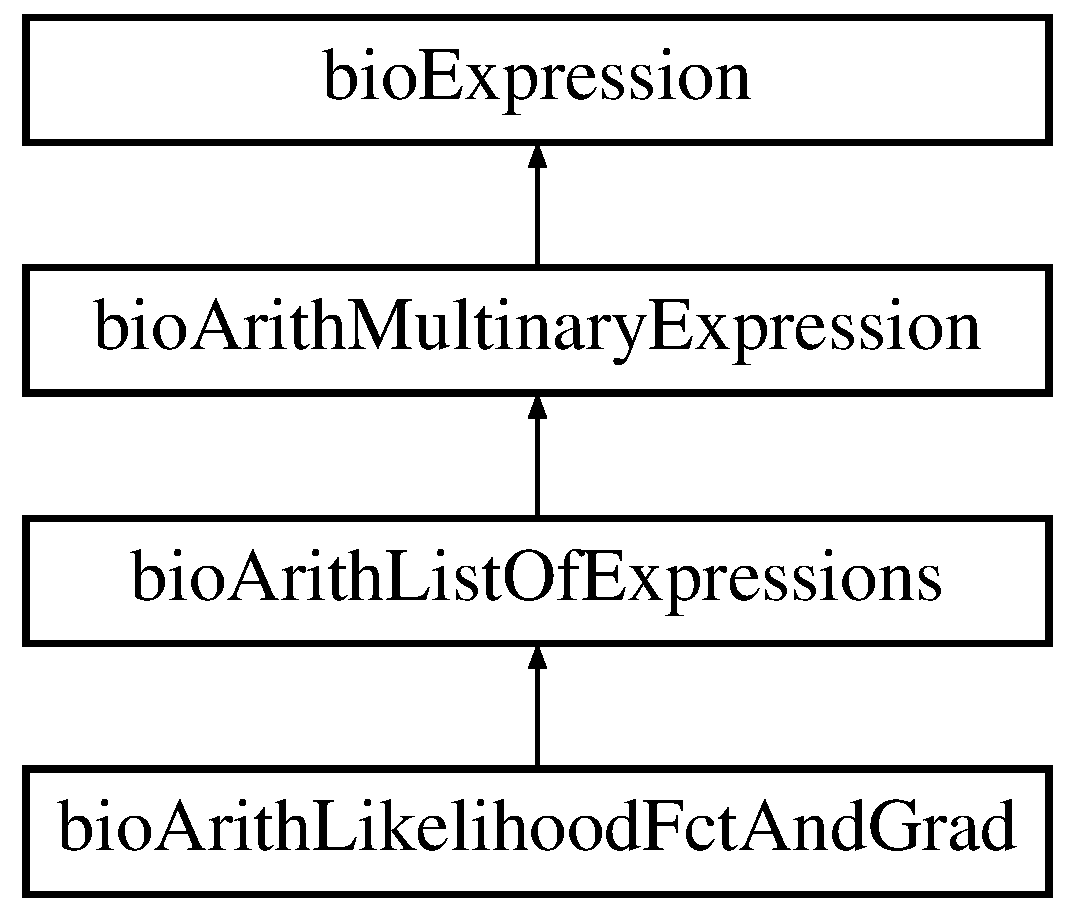
\includegraphics[height=4.000000cm]{classbio_arith_likelihood_fct_and_grad}
\end{center}
\end{figure}
\subsection*{Public Member Functions}
\begin{DoxyCompactItemize}
\item 
\mbox{\Hypertarget{classbio_arith_likelihood_fct_and_grad_aa06f8d73f968bd6ade48202ac8d575c1}\label{classbio_arith_likelihood_fct_and_grad_aa06f8d73f968bd6ade48202ac8d575c1}} 
{\bfseries bio\+Arith\+Likelihood\+Fct\+And\+Grad} (pat\+U\+Long par, pat\+String a\+Iter, vector$<$ pat\+U\+Long $>$ fg, pat\+Error $\ast$\&err)
\item 
\mbox{\Hypertarget{classbio_arith_likelihood_fct_and_grad_a0dd5a4ad701db88338deffefe79a3101}\label{classbio_arith_likelihood_fct_and_grad_a0dd5a4ad701db88338deffefe79a3101}} 
virtual vector$<$ pat\+Real $>$ {\bfseries get\+Values} (pat\+Error $\ast$\&err) const
\item 
virtual pat\+String \hyperlink{classbio_arith_likelihood_fct_and_grad_ad181305327744af1de885d4169888378}{get\+Operator\+Name} () const
\item 
virtual \hyperlink{classbio_expression}{bio\+Expression} $\ast$ \hyperlink{classbio_arith_likelihood_fct_and_grad_ab814e1cc11e481c88ba1d7401432c706}{get\+Derivative} (pat\+U\+Long a\+Literal\+Id, pat\+Error $\ast$\&err) const
\item 
virtual \hyperlink{classbio_arith_likelihood_fct_and_grad}{bio\+Arith\+Likelihood\+Fct\+And\+Grad} $\ast$ \hyperlink{classbio_arith_likelihood_fct_and_grad_a053e08511308e3c8a3e572f5c5f8f019}{get\+Deep\+Copy} (\hyperlink{classbio_expression_repository}{bio\+Expression\+Repository} $\ast$rep, pat\+Error $\ast$\&err) const
\item 
virtual pat\+String \hyperlink{classbio_arith_likelihood_fct_and_grad_ae264b073115dcff703cf2b7926384976}{get\+Expression} (pat\+Error $\ast$\&err) const
\item 
\mbox{\Hypertarget{classbio_arith_likelihood_fct_and_grad_ad8862028e61ef7316833398e7ec3ff0c}\label{classbio_arith_likelihood_fct_and_grad_ad8862028e61ef7316833398e7ec3ff0c}} 
virtual pat\+U\+Long {\bfseries get\+Number\+Of\+Operations} () const
\item 
virtual pat\+String \hyperlink{classbio_arith_likelihood_fct_and_grad_ab7df38cb82ae1a9b77d51445931e1ac9}{the\+Iterator} () const
\item 
virtual pat\+String \hyperlink{classbio_arith_likelihood_fct_and_grad_a5f34a72c24f6d3e7215e82b2b9843e19}{get\+Expression\+String} () const
\item 
\mbox{\Hypertarget{classbio_arith_likelihood_fct_and_grad_aa6d439996e243a4ef15f92ac9e426aef}\label{classbio_arith_likelihood_fct_and_grad_aa6d439996e243a4ef15f92ac9e426aef}} 
pat\+Boolean {\bfseries contains\+An\+Iterator} () const
\end{DoxyCompactItemize}
\subsection*{Additional Inherited Members}


\subsection{Detailed Description}
Class implementing an iterator on a list of expressions. Note that, mathematically, a list of sums is equivalent to a sum of lists. But this class is designed to keep the structure of the sum, necessary to compute the B\+H\+HH, which requires the gradient for each element of the sum. This is typically required for a loglikelihood function, so the name. 

\subsection{Member Function Documentation}
\mbox{\Hypertarget{classbio_arith_likelihood_fct_and_grad_a053e08511308e3c8a3e572f5c5f8f019}\label{classbio_arith_likelihood_fct_and_grad_a053e08511308e3c8a3e572f5c5f8f019}} 
\index{bio\+Arith\+Likelihood\+Fct\+And\+Grad@{bio\+Arith\+Likelihood\+Fct\+And\+Grad}!get\+Deep\+Copy@{get\+Deep\+Copy}}
\index{get\+Deep\+Copy@{get\+Deep\+Copy}!bio\+Arith\+Likelihood\+Fct\+And\+Grad@{bio\+Arith\+Likelihood\+Fct\+And\+Grad}}
\subsubsection{\texorpdfstring{get\+Deep\+Copy()}{getDeepCopy()}}
{\footnotesize\ttfamily \hyperlink{classbio_arith_likelihood_fct_and_grad}{bio\+Arith\+Likelihood\+Fct\+And\+Grad} $\ast$ bio\+Arith\+Likelihood\+Fct\+And\+Grad\+::get\+Deep\+Copy (\begin{DoxyParamCaption}\item[{\hyperlink{classbio_expression_repository}{bio\+Expression\+Repository} $\ast$}]{rep,  }\item[{pat\+Error $\ast$\&}]{err }\end{DoxyParamCaption}) const\hspace{0.3cm}{\ttfamily [virtual]}}

Create a deep copy of the expression and returns a pointer to it. It means that new instances of the children are created. 

Reimplemented from \hyperlink{classbio_arith_list_of_expressions_af13c0c6710776c02d3f7c0e27d5cd724}{bio\+Arith\+List\+Of\+Expressions}.

\mbox{\Hypertarget{classbio_arith_likelihood_fct_and_grad_ab814e1cc11e481c88ba1d7401432c706}\label{classbio_arith_likelihood_fct_and_grad_ab814e1cc11e481c88ba1d7401432c706}} 
\index{bio\+Arith\+Likelihood\+Fct\+And\+Grad@{bio\+Arith\+Likelihood\+Fct\+And\+Grad}!get\+Derivative@{get\+Derivative}}
\index{get\+Derivative@{get\+Derivative}!bio\+Arith\+Likelihood\+Fct\+And\+Grad@{bio\+Arith\+Likelihood\+Fct\+And\+Grad}}
\subsubsection{\texorpdfstring{get\+Derivative()}{getDerivative()}}
{\footnotesize\ttfamily \hyperlink{classbio_expression}{bio\+Expression} $\ast$ bio\+Arith\+Likelihood\+Fct\+And\+Grad\+::get\+Derivative (\begin{DoxyParamCaption}\item[{pat\+U\+Long}]{a\+Literal\+Id,  }\item[{pat\+Error $\ast$\&}]{err }\end{DoxyParamCaption}) const\hspace{0.3cm}{\ttfamily [virtual]}}

\begin{DoxyReturn}{Returns}
value of the derivative w.\+r.\+t literal 
\end{DoxyReturn}

\begin{DoxyParams}{Parameters}
{\em index} & of the literal involved in the derivative \\
\hline
{\em err} & ref. of the pointer to the error object. \\
\hline
\end{DoxyParams}


Reimplemented from \hyperlink{classbio_arith_list_of_expressions_a14fe977b86bc69c4b3afe59d44b6c03f}{bio\+Arith\+List\+Of\+Expressions}.

\mbox{\Hypertarget{classbio_arith_likelihood_fct_and_grad_ae264b073115dcff703cf2b7926384976}\label{classbio_arith_likelihood_fct_and_grad_ae264b073115dcff703cf2b7926384976}} 
\index{bio\+Arith\+Likelihood\+Fct\+And\+Grad@{bio\+Arith\+Likelihood\+Fct\+And\+Grad}!get\+Expression@{get\+Expression}}
\index{get\+Expression@{get\+Expression}!bio\+Arith\+Likelihood\+Fct\+And\+Grad@{bio\+Arith\+Likelihood\+Fct\+And\+Grad}}
\subsubsection{\texorpdfstring{get\+Expression()}{getExpression()}}
{\footnotesize\ttfamily pat\+String bio\+Arith\+Likelihood\+Fct\+And\+Grad\+::get\+Expression (\begin{DoxyParamCaption}\item[{pat\+Error $\ast$\&}]{err }\end{DoxyParamCaption}) const\hspace{0.3cm}{\ttfamily [virtual]}}

\begin{DoxyReturn}{Returns}
printed expression 
\end{DoxyReturn}


Reimplemented from \hyperlink{classbio_arith_multinary_expression_a769ab218dc1f1efcdaf3204da0ecc705}{bio\+Arith\+Multinary\+Expression}.

\mbox{\Hypertarget{classbio_arith_likelihood_fct_and_grad_a5f34a72c24f6d3e7215e82b2b9843e19}\label{classbio_arith_likelihood_fct_and_grad_a5f34a72c24f6d3e7215e82b2b9843e19}} 
\index{bio\+Arith\+Likelihood\+Fct\+And\+Grad@{bio\+Arith\+Likelihood\+Fct\+And\+Grad}!get\+Expression\+String@{get\+Expression\+String}}
\index{get\+Expression\+String@{get\+Expression\+String}!bio\+Arith\+Likelihood\+Fct\+And\+Grad@{bio\+Arith\+Likelihood\+Fct\+And\+Grad}}
\subsubsection{\texorpdfstring{get\+Expression\+String()}{getExpressionString()}}
{\footnotesize\ttfamily pat\+String bio\+Arith\+Likelihood\+Fct\+And\+Grad\+::get\+Expression\+String (\begin{DoxyParamCaption}{ }\end{DoxyParamCaption}) const\hspace{0.3cm}{\ttfamily [virtual]}}

Compute a string that represents the expression. It is designed to replace the expression itself when used only for comparison purposes. Code\+: +\{expr1\}\{expr2\}\+: binary plus -\/\{expr1\}\{expr2\}\+: binary minus \{expr1\}\{expr2\}\+: multiplication /\{expr1\}\{expr2\}\+: division $^\wedge$\{expr1\}\{expr2\}\+: power \&\{expr1\}\{expr2\}\+: and $\vert$\{expr1\}\{expr2\}\+: or =\{expr1\}\{expr2\}\+: equal !=\{expr1\}\{expr2\}\+: not equal $<$\{expr1\}\{expr2\}\+: lesser than $<$=\{expr1\}\{expr2\}\+: lesser or equal to $>$\{expr1\}\{expr2\}\+: greater than $>$=\{expr1\}\{expr2\}\+: greater or equal to \$A\{expr\}\+: abs \$D\mbox{[}expr\mbox{]}\mbox{[}\{expr1\}...\{exprN\}\mbox{]}\+: dictionary (\hyperlink{classbio_arith_elem}{bio\+Arith\+Elem}) \$E\{expr\}\+: exp \$L\{expr\}\+: log \$M\{expr\}\+: Unary minus \$\+Piterator\+\_\+name\{expr\}\+: prod \$Q\{string1\}\{string2\}\+: sequence \$\+Siterator\+\_\+name\{expr\}\+: sum \$\+Ziterator\+\_\+name\mbox{[}\{expr1\}...\{exprN\}\mbox{]}\+: merged sum \{expr1\}\{expr2\}...\{exprN\}//\+: list of expressions number\+: constant \#id\+: literal \&id\+: random 

Reimplemented from \hyperlink{classbio_arith_list_of_expressions_ac6a8b9493bc91520a1882df3cddc383d}{bio\+Arith\+List\+Of\+Expressions}.

\mbox{\Hypertarget{classbio_arith_likelihood_fct_and_grad_ad181305327744af1de885d4169888378}\label{classbio_arith_likelihood_fct_and_grad_ad181305327744af1de885d4169888378}} 
\index{bio\+Arith\+Likelihood\+Fct\+And\+Grad@{bio\+Arith\+Likelihood\+Fct\+And\+Grad}!get\+Operator\+Name@{get\+Operator\+Name}}
\index{get\+Operator\+Name@{get\+Operator\+Name}!bio\+Arith\+Likelihood\+Fct\+And\+Grad@{bio\+Arith\+Likelihood\+Fct\+And\+Grad}}
\subsubsection{\texorpdfstring{get\+Operator\+Name()}{getOperatorName()}}
{\footnotesize\ttfamily pat\+String bio\+Arith\+Likelihood\+Fct\+And\+Grad\+::get\+Operator\+Name (\begin{DoxyParamCaption}{ }\end{DoxyParamCaption}) const\hspace{0.3cm}{\ttfamily [virtual]}}

\begin{DoxyReturn}{Returns}
name of the operator 
\end{DoxyReturn}


Reimplemented from \hyperlink{classbio_arith_list_of_expressions_af0c6e016d69454ac0b7d4f889190807e}{bio\+Arith\+List\+Of\+Expressions}.

\mbox{\Hypertarget{classbio_arith_likelihood_fct_and_grad_ab7df38cb82ae1a9b77d51445931e1ac9}\label{classbio_arith_likelihood_fct_and_grad_ab7df38cb82ae1a9b77d51445931e1ac9}} 
\index{bio\+Arith\+Likelihood\+Fct\+And\+Grad@{bio\+Arith\+Likelihood\+Fct\+And\+Grad}!the\+Iterator@{the\+Iterator}}
\index{the\+Iterator@{the\+Iterator}!bio\+Arith\+Likelihood\+Fct\+And\+Grad@{bio\+Arith\+Likelihood\+Fct\+And\+Grad}}
\subsubsection{\texorpdfstring{the\+Iterator()}{theIterator()}}
{\footnotesize\ttfamily pat\+String bio\+Arith\+Likelihood\+Fct\+And\+Grad\+::the\+Iterator (\begin{DoxyParamCaption}{ }\end{DoxyParamCaption}) const\hspace{0.3cm}{\ttfamily [virtual]}}

\begin{DoxyReturn}{Returns}
pointer to the iterator information if the top level node is an iterator, N\+U\+LL otherwise. Not recursive. 
\end{DoxyReturn}


Reimplemented from \hyperlink{classbio_expression_a9830c0cf012012c811b826adc54291f6}{bio\+Expression}.



The documentation for this class was generated from the following files\+:\begin{DoxyCompactItemize}
\item 
bio\+Arith\+Likelihood\+Fct\+And\+Grad.\+h\item 
bio\+Arith\+Likelihood\+Fct\+And\+Grad.\+cc\end{DoxyCompactItemize}

\hypertarget{classbio_arith_list_of_expressions}{}\section{bio\+Arith\+List\+Of\+Expressions Class Reference}
\label{classbio_arith_list_of_expressions}\index{bio\+Arith\+List\+Of\+Expressions@{bio\+Arith\+List\+Of\+Expressions}}
Inheritance diagram for bio\+Arith\+List\+Of\+Expressions\+:\begin{figure}[H]
\begin{center}
\leavevmode
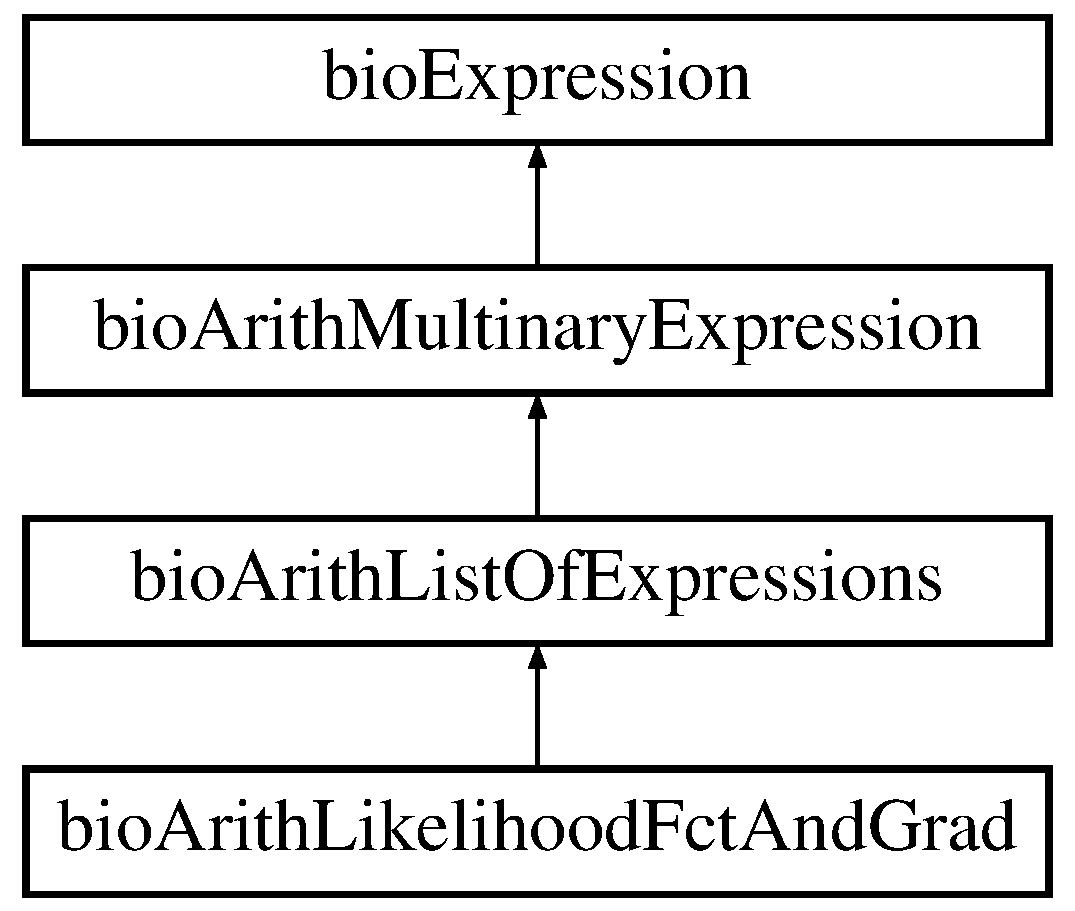
\includegraphics[height=4.000000cm]{classbio_arith_list_of_expressions}
\end{center}
\end{figure}
\subsection*{Public Member Functions}
\begin{DoxyCompactItemize}
\item 
\mbox{\Hypertarget{classbio_arith_list_of_expressions_a6ed575066b9d2f8acb4edc914cb743b9}\label{classbio_arith_list_of_expressions_a6ed575066b9d2f8acb4edc914cb743b9}} 
{\bfseries bio\+Arith\+List\+Of\+Expressions} (pat\+U\+Long par, vector$<$ pat\+U\+Long $>$ l)
\item 
\mbox{\Hypertarget{classbio_arith_list_of_expressions_ae6f687023278e7369c6c922c11275375}\label{classbio_arith_list_of_expressions_ae6f687023278e7369c6c922c11275375}} 
tr\+Hessian $\ast$ {\bfseries get\+Bhhh} ()
\item 
\mbox{\Hypertarget{classbio_arith_list_of_expressions_a4c5a136ef5028e8e8dc4ada39195d87f}\label{classbio_arith_list_of_expressions_a4c5a136ef5028e8e8dc4ada39195d87f}} 
virtual vector$<$ pat\+Real $>$ {\bfseries get\+Values} (pat\+Error $\ast$\&err) const
\item 
virtual pat\+String \hyperlink{classbio_arith_list_of_expressions_af0c6e016d69454ac0b7d4f889190807e}{get\+Operator\+Name} () const
\item 
\mbox{\Hypertarget{classbio_arith_list_of_expressions_a12892de13bdd862f8671bad5dab68394}\label{classbio_arith_list_of_expressions_a12892de13bdd862f8671bad5dab68394}} 
virtual pat\+Real {\bfseries get\+Value} (pat\+Error $\ast$\&err) const
\item 
virtual \hyperlink{classbio_expression}{bio\+Expression} $\ast$ \hyperlink{classbio_arith_list_of_expressions_a14fe977b86bc69c4b3afe59d44b6c03f}{get\+Derivative} (pat\+U\+Long a\+Literal\+Id, pat\+Error $\ast$\&err) const
\item 
virtual \hyperlink{classbio_arith_list_of_expressions}{bio\+Arith\+List\+Of\+Expressions} $\ast$ \hyperlink{classbio_arith_list_of_expressions_af13c0c6710776c02d3f7c0e27d5cd724}{get\+Deep\+Copy} (\hyperlink{classbio_expression_repository}{bio\+Expression\+Repository} $\ast$rep, pat\+Error $\ast$\&err) const
\item 
virtual \hyperlink{classbio_arith_list_of_expressions}{bio\+Arith\+List\+Of\+Expressions} $\ast$ \hyperlink{classbio_arith_list_of_expressions_afd5867cdac9cea54a704a075412b3c08}{get\+Shallow\+Copy} (\hyperlink{classbio_expression_repository}{bio\+Expression\+Repository} $\ast$rep, pat\+Error $\ast$\&err) const
\item 
virtual pat\+String \hyperlink{classbio_arith_list_of_expressions_ac6a8b9493bc91520a1882df3cddc383d}{get\+Expression\+String} () const
\item 
\mbox{\Hypertarget{classbio_arith_list_of_expressions_a22bfedcbe9c678289be1e8040a73a8ca}\label{classbio_arith_list_of_expressions_a22bfedcbe9c678289be1e8040a73a8ca}} 
virtual \hyperlink{classbio_arith_list_of_expressions}{bio\+Arith\+List\+Of\+Expressions} $\ast$ {\bfseries get\+Function\+And\+Derivatives} (vector$<$ pat\+U\+Long $>$ literal\+Ids, pat\+Error $\ast$\&err) const
\end{DoxyCompactItemize}
\subsection*{Protected Attributes}
\begin{DoxyCompactItemize}
\item 
\mbox{\Hypertarget{classbio_arith_list_of_expressions_ad1c126ae53fc25558593738125005374}\label{classbio_arith_list_of_expressions_ad1c126ae53fc25558593738125005374}} 
tr\+Hessian $\ast$ {\bfseries bhhh}
\end{DoxyCompactItemize}


\subsection{Member Function Documentation}
\mbox{\Hypertarget{classbio_arith_list_of_expressions_af13c0c6710776c02d3f7c0e27d5cd724}\label{classbio_arith_list_of_expressions_af13c0c6710776c02d3f7c0e27d5cd724}} 
\index{bio\+Arith\+List\+Of\+Expressions@{bio\+Arith\+List\+Of\+Expressions}!get\+Deep\+Copy@{get\+Deep\+Copy}}
\index{get\+Deep\+Copy@{get\+Deep\+Copy}!bio\+Arith\+List\+Of\+Expressions@{bio\+Arith\+List\+Of\+Expressions}}
\subsubsection{\texorpdfstring{get\+Deep\+Copy()}{getDeepCopy()}}
{\footnotesize\ttfamily \hyperlink{classbio_arith_list_of_expressions}{bio\+Arith\+List\+Of\+Expressions} $\ast$ bio\+Arith\+List\+Of\+Expressions\+::get\+Deep\+Copy (\begin{DoxyParamCaption}\item[{\hyperlink{classbio_expression_repository}{bio\+Expression\+Repository} $\ast$}]{rep,  }\item[{pat\+Error $\ast$\&}]{err }\end{DoxyParamCaption}) const\hspace{0.3cm}{\ttfamily [virtual]}}

Create a deep copy of the expression and returns a pointer to it. It means that new instances of the children are created. 

Reimplemented from \hyperlink{classbio_expression_a4ee1b8add634078a02eaae26cd40dcc8}{bio\+Expression}.



Reimplemented in \hyperlink{classbio_arith_likelihood_fct_and_grad_a053e08511308e3c8a3e572f5c5f8f019}{bio\+Arith\+Likelihood\+Fct\+And\+Grad}.

\mbox{\Hypertarget{classbio_arith_list_of_expressions_a14fe977b86bc69c4b3afe59d44b6c03f}\label{classbio_arith_list_of_expressions_a14fe977b86bc69c4b3afe59d44b6c03f}} 
\index{bio\+Arith\+List\+Of\+Expressions@{bio\+Arith\+List\+Of\+Expressions}!get\+Derivative@{get\+Derivative}}
\index{get\+Derivative@{get\+Derivative}!bio\+Arith\+List\+Of\+Expressions@{bio\+Arith\+List\+Of\+Expressions}}
\subsubsection{\texorpdfstring{get\+Derivative()}{getDerivative()}}
{\footnotesize\ttfamily \hyperlink{classbio_expression}{bio\+Expression} $\ast$ bio\+Arith\+List\+Of\+Expressions\+::get\+Derivative (\begin{DoxyParamCaption}\item[{pat\+U\+Long}]{a\+Literal\+Id,  }\item[{pat\+Error $\ast$\&}]{err }\end{DoxyParamCaption}) const\hspace{0.3cm}{\ttfamily [virtual]}}

\begin{DoxyReturn}{Returns}
value of the derivative w.\+r.\+t literal 
\end{DoxyReturn}

\begin{DoxyParams}{Parameters}
{\em index} & of the literal involved in the derivative \\
\hline
{\em err} & ref. of the pointer to the error object. \\
\hline
\end{DoxyParams}


Reimplemented from \hyperlink{classbio_expression_a5915579d1193f25f216c1e273c97f2ce}{bio\+Expression}.



Reimplemented in \hyperlink{classbio_arith_likelihood_fct_and_grad_ab814e1cc11e481c88ba1d7401432c706}{bio\+Arith\+Likelihood\+Fct\+And\+Grad}.

\mbox{\Hypertarget{classbio_arith_list_of_expressions_ac6a8b9493bc91520a1882df3cddc383d}\label{classbio_arith_list_of_expressions_ac6a8b9493bc91520a1882df3cddc383d}} 
\index{bio\+Arith\+List\+Of\+Expressions@{bio\+Arith\+List\+Of\+Expressions}!get\+Expression\+String@{get\+Expression\+String}}
\index{get\+Expression\+String@{get\+Expression\+String}!bio\+Arith\+List\+Of\+Expressions@{bio\+Arith\+List\+Of\+Expressions}}
\subsubsection{\texorpdfstring{get\+Expression\+String()}{getExpressionString()}}
{\footnotesize\ttfamily pat\+String bio\+Arith\+List\+Of\+Expressions\+::get\+Expression\+String (\begin{DoxyParamCaption}{ }\end{DoxyParamCaption}) const\hspace{0.3cm}{\ttfamily [virtual]}}

Compute a string that represents the expression. It is designed to replace the expression itself when used only for comparison purposes. Code\+: +\{expr1\}\{expr2\}\+: binary plus -\/\{expr1\}\{expr2\}\+: binary minus \{expr1\}\{expr2\}\+: multiplication /\{expr1\}\{expr2\}\+: division $^\wedge$\{expr1\}\{expr2\}\+: power \&\{expr1\}\{expr2\}\+: and $\vert$\{expr1\}\{expr2\}\+: or =\{expr1\}\{expr2\}\+: equal !=\{expr1\}\{expr2\}\+: not equal $<$\{expr1\}\{expr2\}\+: lesser than $<$=\{expr1\}\{expr2\}\+: lesser or equal to $>$\{expr1\}\{expr2\}\+: greater than $>$=\{expr1\}\{expr2\}\+: greater or equal to \$A\{expr\}\+: abs \$D\mbox{[}expr\mbox{]}\mbox{[}\{expr1\}...\{exprN\}\mbox{]}\+: dictionary (\hyperlink{classbio_arith_elem}{bio\+Arith\+Elem}) \$E\{expr\}\+: exp \$L\{expr\}\+: log \$M\{expr\}\+: Unary minus \$\+Piterator\+\_\+name\{expr\}\+: prod \$Q\{string1\}\{string2\}\+: sequence \$\+Siterator\+\_\+name\{expr\}\+: sum \$\+Ziterator\+\_\+name\mbox{[}\{expr1\}...\{exprN\}\mbox{]}\+: merged sum \{expr1\}\{expr2\}...\{exprN\}//\+: list of expressions number\+: constant \#id\+: literal \&id\+: random 

Reimplemented from \hyperlink{classbio_expression_a3e4b4dca58dbbc6f0e411b30eb3f60b4}{bio\+Expression}.



Reimplemented in \hyperlink{classbio_arith_likelihood_fct_and_grad_a5f34a72c24f6d3e7215e82b2b9843e19}{bio\+Arith\+Likelihood\+Fct\+And\+Grad}.

\mbox{\Hypertarget{classbio_arith_list_of_expressions_af0c6e016d69454ac0b7d4f889190807e}\label{classbio_arith_list_of_expressions_af0c6e016d69454ac0b7d4f889190807e}} 
\index{bio\+Arith\+List\+Of\+Expressions@{bio\+Arith\+List\+Of\+Expressions}!get\+Operator\+Name@{get\+Operator\+Name}}
\index{get\+Operator\+Name@{get\+Operator\+Name}!bio\+Arith\+List\+Of\+Expressions@{bio\+Arith\+List\+Of\+Expressions}}
\subsubsection{\texorpdfstring{get\+Operator\+Name()}{getOperatorName()}}
{\footnotesize\ttfamily pat\+String bio\+Arith\+List\+Of\+Expressions\+::get\+Operator\+Name (\begin{DoxyParamCaption}{ }\end{DoxyParamCaption}) const\hspace{0.3cm}{\ttfamily [virtual]}}

\begin{DoxyReturn}{Returns}
name of the operator 
\end{DoxyReturn}


Reimplemented from \hyperlink{classbio_expression_a2353a4afb3a2b0af7c63aba086a72bde}{bio\+Expression}.



Reimplemented in \hyperlink{classbio_arith_likelihood_fct_and_grad_ad181305327744af1de885d4169888378}{bio\+Arith\+Likelihood\+Fct\+And\+Grad}.

\mbox{\Hypertarget{classbio_arith_list_of_expressions_afd5867cdac9cea54a704a075412b3c08}\label{classbio_arith_list_of_expressions_afd5867cdac9cea54a704a075412b3c08}} 
\index{bio\+Arith\+List\+Of\+Expressions@{bio\+Arith\+List\+Of\+Expressions}!get\+Shallow\+Copy@{get\+Shallow\+Copy}}
\index{get\+Shallow\+Copy@{get\+Shallow\+Copy}!bio\+Arith\+List\+Of\+Expressions@{bio\+Arith\+List\+Of\+Expressions}}
\subsubsection{\texorpdfstring{get\+Shallow\+Copy()}{getShallowCopy()}}
{\footnotesize\ttfamily virtual \hyperlink{classbio_arith_list_of_expressions}{bio\+Arith\+List\+Of\+Expressions}$\ast$ bio\+Arith\+List\+Of\+Expressions\+::get\+Shallow\+Copy (\begin{DoxyParamCaption}\item[{\hyperlink{classbio_expression_repository}{bio\+Expression\+Repository} $\ast$}]{rep,  }\item[{pat\+Error $\ast$\&}]{err }\end{DoxyParamCaption}) const\hspace{0.3cm}{\ttfamily [virtual]}}

Create a shallow copy of the expression and returns a pointer to it. It means that no new instance of the children are created. It is typically called by the repository 

Reimplemented from \hyperlink{classbio_expression_a442534762693b92baaf33928979a1bf8}{bio\+Expression}.



The documentation for this class was generated from the following files\+:\begin{DoxyCompactItemize}
\item 
bio\+Arith\+List\+Of\+Expressions.\+h\item 
bio\+Arith\+List\+Of\+Expressions.\+cc\end{DoxyCompactItemize}

\hypertarget{classbio_arith_literal}{}\section{bio\+Arith\+Literal Class Reference}
\label{classbio_arith_literal}\index{bio\+Arith\+Literal@{bio\+Arith\+Literal}}


{\ttfamily \#include $<$bio\+Arith\+Literal.\+h$>$}

Inheritance diagram for bio\+Arith\+Literal\+:\begin{figure}[H]
\begin{center}
\leavevmode
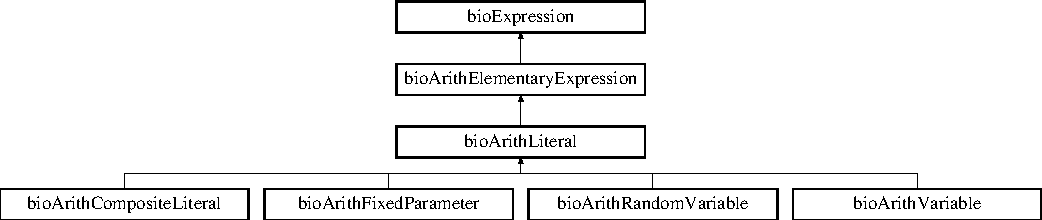
\includegraphics[height=2.962963cm]{classbio_arith_literal}
\end{center}
\end{figure}
\subsection*{Public Member Functions}
\begin{DoxyCompactItemize}
\item 
\mbox{\Hypertarget{classbio_arith_literal_af66772afce990e444ee7d68d3b2b5144}\label{classbio_arith_literal_af66772afce990e444ee7d68d3b2b5144}} 
{\bfseries bio\+Arith\+Literal} (\hyperlink{classbio_expression_repository}{bio\+Expression\+Repository} $\ast$rep, pat\+U\+Long par, pat\+U\+Long the\+Literal\+Id)
\item 
virtual pat\+String \hyperlink{classbio_arith_literal_a0cdf0cb347fbf2b6db50b31ef8824d9c}{get\+Operator\+Name} () const
\item 
virtual \hyperlink{classbio_expression}{bio\+Expression} $\ast$ \hyperlink{classbio_arith_literal_affebfbf01e421ec9cf55b4cf883039ce}{get\+Derivative} (pat\+U\+Long a\+Literal\+Id, pat\+Error $\ast$\&err) const
\item 
\mbox{\Hypertarget{classbio_arith_literal_ac348b105f8b4d5f36b2c8b88ce5c8a97}\label{classbio_arith_literal_ac348b105f8b4d5f36b2c8b88ce5c8a97}} 
virtual pat\+Boolean {\bfseries depends\+Of} (pat\+U\+Long a\+Literal\+Id) const
\item 
virtual pat\+String \hyperlink{classbio_arith_literal_ae55e7cbd7d3561b56af50fc741009a60}{get\+Expression} (pat\+Error $\ast$\&err) const
\item 
virtual pat\+String \hyperlink{classbio_arith_literal_ab75046eaffcb688b83031da7f91653f9}{get\+Expression\+String} () const
\item 
\mbox{\Hypertarget{classbio_arith_literal_aff6e75c06e5e9a50dcd01590d48262b4}\label{classbio_arith_literal_aff6e75c06e5e9a50dcd01590d48262b4}} 
virtual pat\+Boolean {\bfseries is\+Literal} () const
\item 
virtual \hyperlink{classbio_function_and_derivatives}{bio\+Function\+And\+Derivatives} $\ast$ \hyperlink{classbio_arith_literal_acce01225d50f0ba0a263b2fbaa71b79b}{get\+Numerical\+Function\+And\+Gradient} (vector$<$ pat\+U\+Long $>$ literal\+Ids, pat\+Boolean compute\+Hessian, pat\+Boolean debug\+Derivatives, pat\+Error $\ast$\&err)
\item 
\mbox{\Hypertarget{classbio_arith_literal_aa18cdbbe1c0b9abdbeac945e44aa5c8d}\label{classbio_arith_literal_aa18cdbbe1c0b9abdbeac945e44aa5c8d}} 
virtual pat\+Boolean {\bfseries verify\+Derivatives} (vector$<$ pat\+U\+Long $>$ literal\+Ids, pat\+Error $\ast$\&err)
\end{DoxyCompactItemize}
\subsection*{Protected Attributes}
\begin{DoxyCompactItemize}
\item 
\mbox{\Hypertarget{classbio_arith_literal_a09eb7ed85621c6f987d2a23644839828}\label{classbio_arith_literal_a09eb7ed85621c6f987d2a23644839828}} 
pat\+U\+Long {\bfseries the\+Literal\+Id}
\end{DoxyCompactItemize}


\subsection{Detailed Description}
Class implementing the node for literals in an expression 

\subsection{Member Function Documentation}
\mbox{\Hypertarget{classbio_arith_literal_affebfbf01e421ec9cf55b4cf883039ce}\label{classbio_arith_literal_affebfbf01e421ec9cf55b4cf883039ce}} 
\index{bio\+Arith\+Literal@{bio\+Arith\+Literal}!get\+Derivative@{get\+Derivative}}
\index{get\+Derivative@{get\+Derivative}!bio\+Arith\+Literal@{bio\+Arith\+Literal}}
\subsubsection{\texorpdfstring{get\+Derivative()}{getDerivative()}}
{\footnotesize\ttfamily \hyperlink{classbio_expression}{bio\+Expression} $\ast$ bio\+Arith\+Literal\+::get\+Derivative (\begin{DoxyParamCaption}\item[{pat\+U\+Long}]{a\+Literal\+Id,  }\item[{pat\+Error $\ast$\&}]{err }\end{DoxyParamCaption}) const\hspace{0.3cm}{\ttfamily [virtual]}}

\begin{DoxyReturn}{Returns}
value of the derivative w.\+r.\+t literal 
\end{DoxyReturn}

\begin{DoxyParams}{Parameters}
{\em index} & of the literal involved in the derivative \\
\hline
{\em err} & ref. of the pointer to the error object. \\
\hline
\end{DoxyParams}


Reimplemented from \hyperlink{classbio_expression_a5915579d1193f25f216c1e273c97f2ce}{bio\+Expression}.

\mbox{\Hypertarget{classbio_arith_literal_ae55e7cbd7d3561b56af50fc741009a60}\label{classbio_arith_literal_ae55e7cbd7d3561b56af50fc741009a60}} 
\index{bio\+Arith\+Literal@{bio\+Arith\+Literal}!get\+Expression@{get\+Expression}}
\index{get\+Expression@{get\+Expression}!bio\+Arith\+Literal@{bio\+Arith\+Literal}}
\subsubsection{\texorpdfstring{get\+Expression()}{getExpression()}}
{\footnotesize\ttfamily pat\+String bio\+Arith\+Literal\+::get\+Expression (\begin{DoxyParamCaption}\item[{pat\+Error $\ast$\&}]{err }\end{DoxyParamCaption}) const\hspace{0.3cm}{\ttfamily [virtual]}}

\begin{DoxyReturn}{Returns}
printed expression 
\end{DoxyReturn}


Reimplemented from \hyperlink{classbio_arith_elementary_expression_a9293635c83789f547b5642855f8c8f16}{bio\+Arith\+Elementary\+Expression}.

\mbox{\Hypertarget{classbio_arith_literal_ab75046eaffcb688b83031da7f91653f9}\label{classbio_arith_literal_ab75046eaffcb688b83031da7f91653f9}} 
\index{bio\+Arith\+Literal@{bio\+Arith\+Literal}!get\+Expression\+String@{get\+Expression\+String}}
\index{get\+Expression\+String@{get\+Expression\+String}!bio\+Arith\+Literal@{bio\+Arith\+Literal}}
\subsubsection{\texorpdfstring{get\+Expression\+String()}{getExpressionString()}}
{\footnotesize\ttfamily pat\+String bio\+Arith\+Literal\+::get\+Expression\+String (\begin{DoxyParamCaption}{ }\end{DoxyParamCaption}) const\hspace{0.3cm}{\ttfamily [virtual]}}

Compute a string that represents the expression. It is designed to replace the expression itself when used only for comparison purposes. Code\+: +\{expr1\}\{expr2\}\+: binary plus -\/\{expr1\}\{expr2\}\+: binary minus \{expr1\}\{expr2\}\+: multiplication /\{expr1\}\{expr2\}\+: division $^\wedge$\{expr1\}\{expr2\}\+: power \&\{expr1\}\{expr2\}\+: and $\vert$\{expr1\}\{expr2\}\+: or =\{expr1\}\{expr2\}\+: equal !=\{expr1\}\{expr2\}\+: not equal $<$\{expr1\}\{expr2\}\+: lesser than $<$=\{expr1\}\{expr2\}\+: lesser or equal to $>$\{expr1\}\{expr2\}\+: greater than $>$=\{expr1\}\{expr2\}\+: greater or equal to \$A\{expr\}\+: abs \$D\mbox{[}expr\mbox{]}\mbox{[}\{expr1\}...\{exprN\}\mbox{]}\+: dictionary (\hyperlink{classbio_arith_elem}{bio\+Arith\+Elem}) \$E\{expr\}\+: exp \$L\{expr\}\+: log \$M\{expr\}\+: Unary minus \$\+Piterator\+\_\+name\{expr\}\+: prod \$Q\{string1\}\{string2\}\+: sequence \$\+Siterator\+\_\+name\{expr\}\+: sum \$\+Ziterator\+\_\+name\mbox{[}\{expr1\}...\{exprN\}\mbox{]}\+: merged sum \{expr1\}\{expr2\}...\{exprN\}//\+: list of expressions number\+: constant \#id\+: literal \&id\+: random 

Reimplemented from \hyperlink{classbio_expression_a3e4b4dca58dbbc6f0e411b30eb3f60b4}{bio\+Expression}.

\mbox{\Hypertarget{classbio_arith_literal_acce01225d50f0ba0a263b2fbaa71b79b}\label{classbio_arith_literal_acce01225d50f0ba0a263b2fbaa71b79b}} 
\index{bio\+Arith\+Literal@{bio\+Arith\+Literal}!get\+Numerical\+Function\+And\+Gradient@{get\+Numerical\+Function\+And\+Gradient}}
\index{get\+Numerical\+Function\+And\+Gradient@{get\+Numerical\+Function\+And\+Gradient}!bio\+Arith\+Literal@{bio\+Arith\+Literal}}
\subsubsection{\texorpdfstring{get\+Numerical\+Function\+And\+Gradient()}{getNumericalFunctionAndGradient()}}
{\footnotesize\ttfamily \hyperlink{classbio_function_and_derivatives}{bio\+Function\+And\+Derivatives} $\ast$ bio\+Arith\+Literal\+::get\+Numerical\+Function\+And\+Gradient (\begin{DoxyParamCaption}\item[{vector$<$ pat\+U\+Long $>$}]{literal\+Ids,  }\item[{pat\+Boolean}]{compute\+Hessian,  }\item[{pat\+Boolean}]{debug\+Derivatives,  }\item[{pat\+Error $\ast$\&}]{err }\end{DoxyParamCaption})\hspace{0.3cm}{\ttfamily [virtual]}}

\begin{DoxyReturn}{Returns}
value and gradient of the expression 
\end{DoxyReturn}

\begin{DoxyParams}{Parameters}
{\em err} & ref. of the pointer to the error object. \\
\hline
\end{DoxyParams}


Reimplemented from \hyperlink{classbio_expression_a91c81ce80c9e972c913b10f5f3c1ed13}{bio\+Expression}.

\mbox{\Hypertarget{classbio_arith_literal_a0cdf0cb347fbf2b6db50b31ef8824d9c}\label{classbio_arith_literal_a0cdf0cb347fbf2b6db50b31ef8824d9c}} 
\index{bio\+Arith\+Literal@{bio\+Arith\+Literal}!get\+Operator\+Name@{get\+Operator\+Name}}
\index{get\+Operator\+Name@{get\+Operator\+Name}!bio\+Arith\+Literal@{bio\+Arith\+Literal}}
\subsubsection{\texorpdfstring{get\+Operator\+Name()}{getOperatorName()}}
{\footnotesize\ttfamily pat\+String bio\+Arith\+Literal\+::get\+Operator\+Name (\begin{DoxyParamCaption}{ }\end{DoxyParamCaption}) const\hspace{0.3cm}{\ttfamily [virtual]}}

\begin{DoxyReturn}{Returns}
name of the operator 
\end{DoxyReturn}


Reimplemented from \hyperlink{classbio_expression_a2353a4afb3a2b0af7c63aba086a72bde}{bio\+Expression}.



The documentation for this class was generated from the following files\+:\begin{DoxyCompactItemize}
\item 
bio\+Arith\+Literal.\+h\item 
bio\+Arith\+Literal.\+cc\end{DoxyCompactItemize}

\hypertarget{classbio_arith_log}{}\section{bio\+Arith\+Log Class Reference}
\label{classbio_arith_log}\index{bio\+Arith\+Log@{bio\+Arith\+Log}}


{\ttfamily \#include $<$bio\+Arith\+Log.\+h$>$}

Inheritance diagram for bio\+Arith\+Log\+:\begin{figure}[H]
\begin{center}
\leavevmode
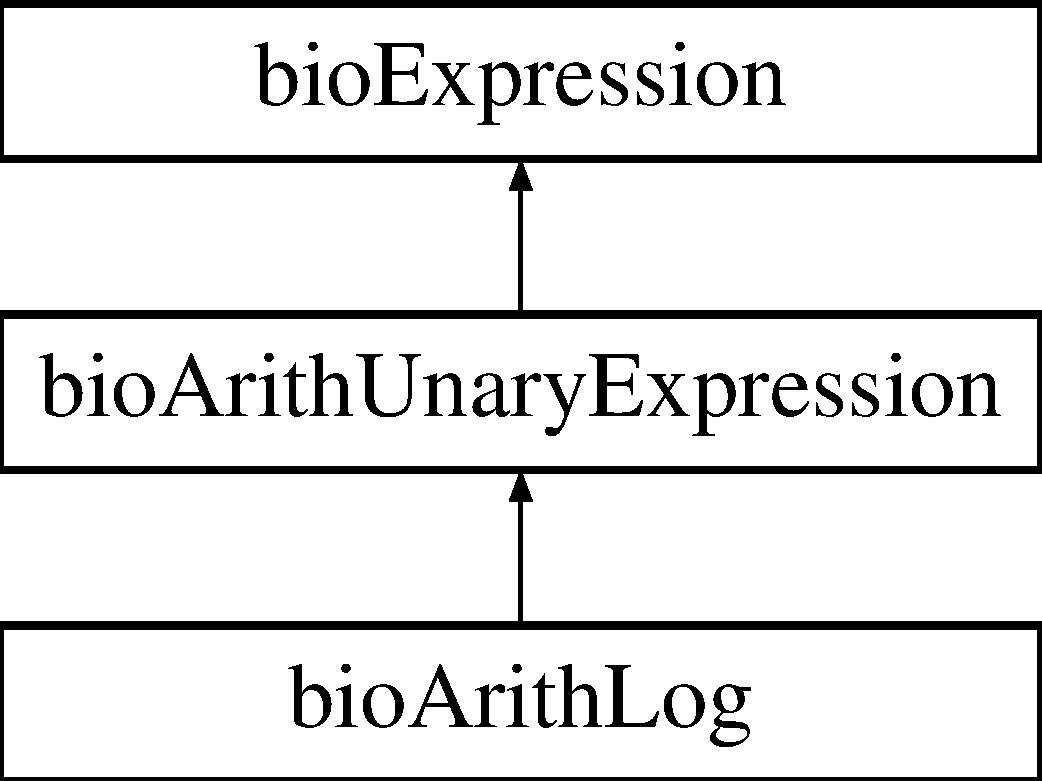
\includegraphics[height=3.000000cm]{classbio_arith_log}
\end{center}
\end{figure}
\subsection*{Public Member Functions}
\begin{DoxyCompactItemize}
\item 
\mbox{\Hypertarget{classbio_arith_log_ae5ac1a21d303fd067ea927f46e41ad5d}\label{classbio_arith_log_ae5ac1a21d303fd067ea927f46e41ad5d}} 
{\bfseries bio\+Arith\+Log} (\hyperlink{classbio_expression_repository}{bio\+Expression\+Repository} $\ast$rep, pat\+U\+Long par, pat\+U\+Long left, pat\+Error $\ast$\&err)
\item 
virtual pat\+String \hyperlink{classbio_arith_log_a730e174a4e9509dccb32c3fab690a46c}{get\+Operator\+Name} () const
\item 
virtual pat\+Real \hyperlink{classbio_arith_log_a31c9d372354ff2f971caffc594c555a9}{get\+Value} (pat\+Boolean prepare\+Gradient, pat\+U\+Long current\+Lap, pat\+Error $\ast$\&err)
\item 
virtual \hyperlink{classbio_expression}{bio\+Expression} $\ast$ \hyperlink{classbio_arith_log_aeb045e82ab8f0c99919b83102d71c527}{get\+Derivative} (pat\+U\+Long a\+Literal, pat\+Error $\ast$\&err) const
\item 
virtual \hyperlink{classbio_arith_log}{bio\+Arith\+Log} $\ast$ \hyperlink{classbio_arith_log_a1717f06ff8d70f5285272ee66c669174}{get\+Deep\+Copy} (\hyperlink{classbio_expression_repository}{bio\+Expression\+Repository} $\ast$rep, pat\+Error $\ast$\&err) const
\item 
virtual \hyperlink{classbio_arith_log}{bio\+Arith\+Log} $\ast$ \hyperlink{classbio_arith_log_aff0739f0c0576b9e70b7192e3e5baf2a}{get\+Shallow\+Copy} (\hyperlink{classbio_expression_repository}{bio\+Expression\+Repository} $\ast$rep, pat\+Error $\ast$\&err) const
\item 
virtual pat\+String \hyperlink{classbio_arith_log_a5deea723cf9e2b50dc4f6c61a6b82090}{get\+Expression\+String} () const
\item 
virtual \hyperlink{classbio_function_and_derivatives}{bio\+Function\+And\+Derivatives} $\ast$ \hyperlink{classbio_arith_log_a875351accd5a515a1d3452dea45a354d}{get\+Numerical\+Function\+And\+Gradient} (vector$<$ pat\+U\+Long $>$ literal\+Ids, pat\+Boolean compute\+Hessian, pat\+Boolean debug\+Derivatives, pat\+Error $\ast$\&err)
\end{DoxyCompactItemize}
\subsection*{Additional Inherited Members}


\subsection{Detailed Description}
Class implementing a node of the tree representing a natural logarithm operation 

\subsection{Member Function Documentation}
\mbox{\Hypertarget{classbio_arith_log_a1717f06ff8d70f5285272ee66c669174}\label{classbio_arith_log_a1717f06ff8d70f5285272ee66c669174}} 
\index{bio\+Arith\+Log@{bio\+Arith\+Log}!get\+Deep\+Copy@{get\+Deep\+Copy}}
\index{get\+Deep\+Copy@{get\+Deep\+Copy}!bio\+Arith\+Log@{bio\+Arith\+Log}}
\subsubsection{\texorpdfstring{get\+Deep\+Copy()}{getDeepCopy()}}
{\footnotesize\ttfamily \hyperlink{classbio_arith_log}{bio\+Arith\+Log} $\ast$ bio\+Arith\+Log\+::get\+Deep\+Copy (\begin{DoxyParamCaption}\item[{\hyperlink{classbio_expression_repository}{bio\+Expression\+Repository} $\ast$}]{rep,  }\item[{pat\+Error $\ast$\&}]{err }\end{DoxyParamCaption}) const\hspace{0.3cm}{\ttfamily [virtual]}}

Create a deep copy of the expression and returns a pointer to it. It means that new instances of the children are created. 

Reimplemented from \hyperlink{classbio_expression_a4ee1b8add634078a02eaae26cd40dcc8}{bio\+Expression}.

\mbox{\Hypertarget{classbio_arith_log_aeb045e82ab8f0c99919b83102d71c527}\label{classbio_arith_log_aeb045e82ab8f0c99919b83102d71c527}} 
\index{bio\+Arith\+Log@{bio\+Arith\+Log}!get\+Derivative@{get\+Derivative}}
\index{get\+Derivative@{get\+Derivative}!bio\+Arith\+Log@{bio\+Arith\+Log}}
\subsubsection{\texorpdfstring{get\+Derivative()}{getDerivative()}}
{\footnotesize\ttfamily \hyperlink{classbio_expression}{bio\+Expression} $\ast$ bio\+Arith\+Log\+::get\+Derivative (\begin{DoxyParamCaption}\item[{pat\+U\+Long}]{a\+Literal\+Id,  }\item[{pat\+Error $\ast$\&}]{err }\end{DoxyParamCaption}) const\hspace{0.3cm}{\ttfamily [virtual]}}

\begin{DoxyReturn}{Returns}
value of the derivative w.\+r.\+t literal 
\end{DoxyReturn}

\begin{DoxyParams}{Parameters}
{\em index} & of the literal involved in the derivative \\
\hline
{\em err} & ref. of the pointer to the error object. \\
\hline
\end{DoxyParams}


Reimplemented from \hyperlink{classbio_expression_a5915579d1193f25f216c1e273c97f2ce}{bio\+Expression}.

\mbox{\Hypertarget{classbio_arith_log_a5deea723cf9e2b50dc4f6c61a6b82090}\label{classbio_arith_log_a5deea723cf9e2b50dc4f6c61a6b82090}} 
\index{bio\+Arith\+Log@{bio\+Arith\+Log}!get\+Expression\+String@{get\+Expression\+String}}
\index{get\+Expression\+String@{get\+Expression\+String}!bio\+Arith\+Log@{bio\+Arith\+Log}}
\subsubsection{\texorpdfstring{get\+Expression\+String()}{getExpressionString()}}
{\footnotesize\ttfamily pat\+String bio\+Arith\+Log\+::get\+Expression\+String (\begin{DoxyParamCaption}{ }\end{DoxyParamCaption}) const\hspace{0.3cm}{\ttfamily [virtual]}}

Compute a string that represents the expression. It is designed to replace the expression itself when used only for comparison purposes. Code\+: +\{expr1\}\{expr2\}\+: binary plus -\/\{expr1\}\{expr2\}\+: binary minus \{expr1\}\{expr2\}\+: multiplication /\{expr1\}\{expr2\}\+: division $^\wedge$\{expr1\}\{expr2\}\+: power \&\{expr1\}\{expr2\}\+: and $\vert$\{expr1\}\{expr2\}\+: or =\{expr1\}\{expr2\}\+: equal !=\{expr1\}\{expr2\}\+: not equal $<$\{expr1\}\{expr2\}\+: lesser than $<$=\{expr1\}\{expr2\}\+: lesser or equal to $>$\{expr1\}\{expr2\}\+: greater than $>$=\{expr1\}\{expr2\}\+: greater or equal to \$A\{expr\}\+: abs \$D\mbox{[}expr\mbox{]}\mbox{[}\{expr1\}...\{exprN\}\mbox{]}\+: dictionary (\hyperlink{classbio_arith_elem}{bio\+Arith\+Elem}) \$E\{expr\}\+: exp \$L\{expr\}\+: log \$M\{expr\}\+: Unary minus \$\+Piterator\+\_\+name\{expr\}\+: prod \$Q\{string1\}\{string2\}\+: sequence \$\+Siterator\+\_\+name\{expr\}\+: sum \$\+Ziterator\+\_\+name\mbox{[}\{expr1\}...\{exprN\}\mbox{]}\+: merged sum \{expr1\}\{expr2\}...\{exprN\}//\+: list of expressions number\+: constant \#id\+: literal \&id\+: random 

Reimplemented from \hyperlink{classbio_expression_a3e4b4dca58dbbc6f0e411b30eb3f60b4}{bio\+Expression}.

\mbox{\Hypertarget{classbio_arith_log_a875351accd5a515a1d3452dea45a354d}\label{classbio_arith_log_a875351accd5a515a1d3452dea45a354d}} 
\index{bio\+Arith\+Log@{bio\+Arith\+Log}!get\+Numerical\+Function\+And\+Gradient@{get\+Numerical\+Function\+And\+Gradient}}
\index{get\+Numerical\+Function\+And\+Gradient@{get\+Numerical\+Function\+And\+Gradient}!bio\+Arith\+Log@{bio\+Arith\+Log}}
\subsubsection{\texorpdfstring{get\+Numerical\+Function\+And\+Gradient()}{getNumericalFunctionAndGradient()}}
{\footnotesize\ttfamily \hyperlink{classbio_function_and_derivatives}{bio\+Function\+And\+Derivatives} $\ast$ bio\+Arith\+Log\+::get\+Numerical\+Function\+And\+Gradient (\begin{DoxyParamCaption}\item[{vector$<$ pat\+U\+Long $>$}]{literal\+Ids,  }\item[{pat\+Boolean}]{compute\+Hessian,  }\item[{pat\+Boolean}]{debug\+Derivatives,  }\item[{pat\+Error $\ast$\&}]{err }\end{DoxyParamCaption})\hspace{0.3cm}{\ttfamily [virtual]}}

\begin{DoxyReturn}{Returns}
value and gradient of the expression 
\end{DoxyReturn}

\begin{DoxyParams}{Parameters}
{\em err} & ref. of the pointer to the error object. \\
\hline
\end{DoxyParams}


Reimplemented from \hyperlink{classbio_expression_a91c81ce80c9e972c913b10f5f3c1ed13}{bio\+Expression}.

\mbox{\Hypertarget{classbio_arith_log_a730e174a4e9509dccb32c3fab690a46c}\label{classbio_arith_log_a730e174a4e9509dccb32c3fab690a46c}} 
\index{bio\+Arith\+Log@{bio\+Arith\+Log}!get\+Operator\+Name@{get\+Operator\+Name}}
\index{get\+Operator\+Name@{get\+Operator\+Name}!bio\+Arith\+Log@{bio\+Arith\+Log}}
\subsubsection{\texorpdfstring{get\+Operator\+Name()}{getOperatorName()}}
{\footnotesize\ttfamily pat\+String bio\+Arith\+Log\+::get\+Operator\+Name (\begin{DoxyParamCaption}{ }\end{DoxyParamCaption}) const\hspace{0.3cm}{\ttfamily [virtual]}}

\begin{DoxyReturn}{Returns}
name of the operator 
\end{DoxyReturn}


Reimplemented from \hyperlink{classbio_expression_a2353a4afb3a2b0af7c63aba086a72bde}{bio\+Expression}.

\mbox{\Hypertarget{classbio_arith_log_aff0739f0c0576b9e70b7192e3e5baf2a}\label{classbio_arith_log_aff0739f0c0576b9e70b7192e3e5baf2a}} 
\index{bio\+Arith\+Log@{bio\+Arith\+Log}!get\+Shallow\+Copy@{get\+Shallow\+Copy}}
\index{get\+Shallow\+Copy@{get\+Shallow\+Copy}!bio\+Arith\+Log@{bio\+Arith\+Log}}
\subsubsection{\texorpdfstring{get\+Shallow\+Copy()}{getShallowCopy()}}
{\footnotesize\ttfamily \hyperlink{classbio_arith_log}{bio\+Arith\+Log} $\ast$ bio\+Arith\+Log\+::get\+Shallow\+Copy (\begin{DoxyParamCaption}\item[{\hyperlink{classbio_expression_repository}{bio\+Expression\+Repository} $\ast$}]{rep,  }\item[{pat\+Error $\ast$\&}]{err }\end{DoxyParamCaption}) const\hspace{0.3cm}{\ttfamily [virtual]}}

Create a shallow copy of the expression and returns a pointer to it. It means that no new instance of the children are created. It is typically called by the repository 

Reimplemented from \hyperlink{classbio_expression_a442534762693b92baaf33928979a1bf8}{bio\+Expression}.

\mbox{\Hypertarget{classbio_arith_log_a31c9d372354ff2f971caffc594c555a9}\label{classbio_arith_log_a31c9d372354ff2f971caffc594c555a9}} 
\index{bio\+Arith\+Log@{bio\+Arith\+Log}!get\+Value@{get\+Value}}
\index{get\+Value@{get\+Value}!bio\+Arith\+Log@{bio\+Arith\+Log}}
\subsubsection{\texorpdfstring{get\+Value()}{getValue()}}
{\footnotesize\ttfamily pat\+Real bio\+Arith\+Log\+::get\+Value (\begin{DoxyParamCaption}\item[{pat\+Boolean}]{prepare\+Gradient,  }\item[{pat\+U\+Long}]{current\+Lap,  }\item[{pat\+Error $\ast$\&}]{err }\end{DoxyParamCaption})\hspace{0.3cm}{\ttfamily [virtual]}}

\begin{DoxyReturn}{Returns}
value of the expression 
\end{DoxyReturn}

\begin{DoxyParams}{Parameters}
{\em err} & ref. of the pointer to the error object. \\
\hline
\end{DoxyParams}


Reimplemented from \hyperlink{classbio_expression_af58662a5d4d456f15bc4f2c9bd4f8a5b}{bio\+Expression}.



The documentation for this class was generated from the following files\+:\begin{DoxyCompactItemize}
\item 
bio\+Arith\+Log.\+h\item 
bio\+Arith\+Log.\+cc\end{DoxyCompactItemize}

\hypertarget{classbio_arith_log_logit}{}\section{bio\+Arith\+Log\+Logit Class Reference}
\label{classbio_arith_log_logit}\index{bio\+Arith\+Log\+Logit@{bio\+Arith\+Log\+Logit}}


{\ttfamily \#include $<$bio\+Arith\+Log\+Logit.\+h$>$}

Inheritance diagram for bio\+Arith\+Log\+Logit\+:\begin{figure}[H]
\begin{center}
\leavevmode
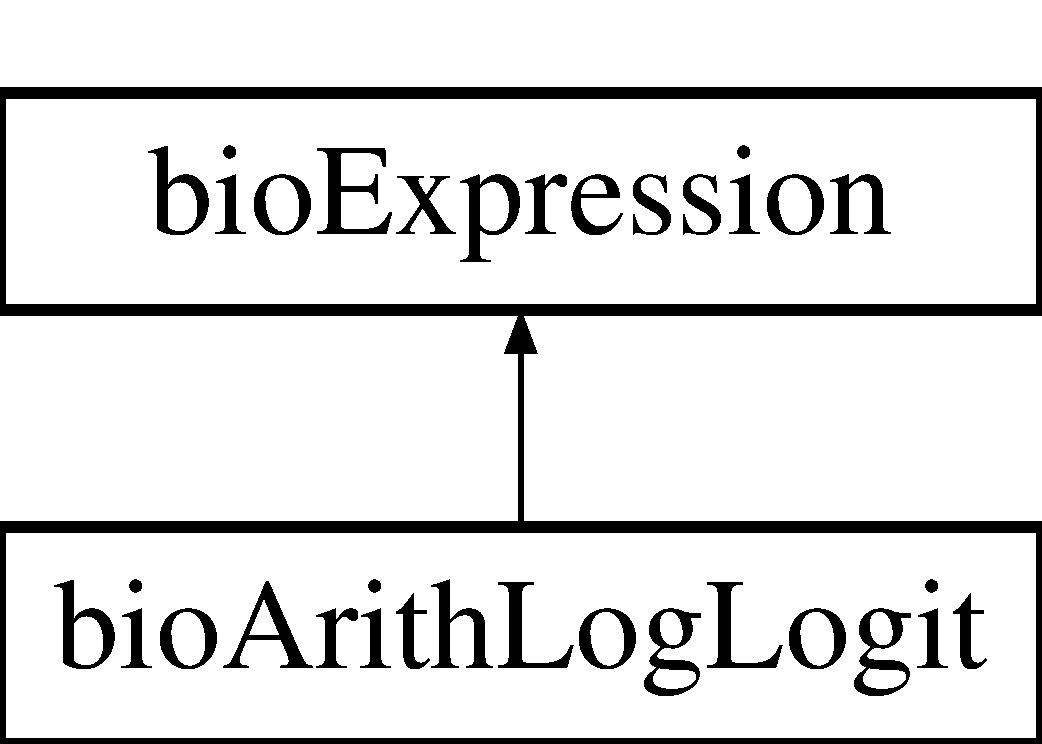
\includegraphics[height=2.000000cm]{classbio_arith_log_logit}
\end{center}
\end{figure}
\subsection*{Public Member Functions}
\begin{DoxyCompactItemize}
\item 
\mbox{\Hypertarget{classbio_arith_log_logit_a42a95d4fa01326e82a4768cc6f6bdcd1}\label{classbio_arith_log_logit_a42a95d4fa01326e82a4768cc6f6bdcd1}} 
{\bfseries bio\+Arith\+Log\+Logit} (\hyperlink{classbio_expression_repository}{bio\+Expression\+Repository} $\ast$rep, pat\+U\+Long par, pat\+U\+Long ind, map$<$ pat\+U\+Long, pat\+U\+Long $>$ a\+Dict, map$<$ pat\+U\+Long, pat\+U\+Long $>$ av\+Dict, pat\+Boolean ll, pat\+Error $\ast$\&err)
\item 
virtual pat\+String \hyperlink{classbio_arith_log_logit_adb9566e06a59ee20cf8b0bc8897b95cd}{get\+Operator\+Name} () const
\item 
virtual pat\+Real \hyperlink{classbio_arith_log_logit_a1d6319d3ce72bda30bc036fdf678e36c}{get\+Value} (pat\+Boolean prepare\+Gradient, pat\+U\+Long current\+Lap, pat\+Error $\ast$\&err)
\item 
virtual \hyperlink{classbio_expression}{bio\+Expression} $\ast$ \hyperlink{classbio_arith_log_logit_a88dd7f743a13f5b836d2c4008d09845f}{get\+Derivative} (pat\+U\+Long a\+Literal\+Id, pat\+Error $\ast$\&err) const
\item 
virtual \hyperlink{classbio_arith_log_logit}{bio\+Arith\+Log\+Logit} $\ast$ \hyperlink{classbio_arith_log_logit_a95be99c67edc6920cea644dcf14c2775}{get\+Deep\+Copy} (\hyperlink{classbio_expression_repository}{bio\+Expression\+Repository} $\ast$rep, pat\+Error $\ast$\&err) const
\item 
virtual \hyperlink{classbio_arith_log_logit}{bio\+Arith\+Log\+Logit} $\ast$ \hyperlink{classbio_arith_log_logit_abf229e9d9897a4f5f0bc3c2e158c24f8}{get\+Shallow\+Copy} (\hyperlink{classbio_expression_repository}{bio\+Expression\+Repository} $\ast$rep, pat\+Error $\ast$\&err) const
\item 
virtual pat\+String \hyperlink{classbio_arith_log_logit_a2683202928e4c00aa06460027a5aa332}{get\+Expression} (pat\+Error $\ast$\&err) const
\item 
\mbox{\Hypertarget{classbio_arith_log_logit_a4c7deadcd687ad799f0e499b697b817c}\label{classbio_arith_log_logit_a4c7deadcd687ad799f0e499b697b817c}} 
virtual pat\+Boolean {\bfseries depends\+Of} (pat\+U\+Long a\+Literal\+Id) const
\item 
\mbox{\Hypertarget{classbio_arith_log_logit_a6cf16644376b4e37d95453e8ccc7fe16}\label{classbio_arith_log_logit_a6cf16644376b4e37d95453e8ccc7fe16}} 
virtual void {\bfseries simplify\+Zeros} (pat\+Error $\ast$\&err)
\item 
\mbox{\Hypertarget{classbio_arith_log_logit_adc9562426b270e7fb3f9b45004232b48}\label{classbio_arith_log_logit_adc9562426b270e7fb3f9b45004232b48}} 
virtual pat\+U\+Long {\bfseries get\+Number\+Of\+Operations} () const
\item 
\mbox{\Hypertarget{classbio_arith_log_logit_ad69939393c7bd316eca7864f16bb5528}\label{classbio_arith_log_logit_ad69939393c7bd316eca7864f16bb5528}} 
pat\+U\+Long {\bfseries last\+Index} () const
\item 
virtual pat\+String \hyperlink{classbio_arith_log_logit_aa769251f7090278fdae9bd7a03670a53}{get\+Expression\+String} () const
\item 
\mbox{\Hypertarget{classbio_arith_log_logit_ab6da440fa9bd5c36b8a7bedc780625f4}\label{classbio_arith_log_logit_ab6da440fa9bd5c36b8a7bedc780625f4}} 
pat\+Boolean {\bfseries contains\+An\+Integral} () const
\item 
\mbox{\Hypertarget{classbio_arith_log_logit_a71ac9387000056545590c68a4235ad62}\label{classbio_arith_log_logit_a71ac9387000056545590c68a4235ad62}} 
pat\+Boolean {\bfseries contains\+An\+Iterator} () const
\item 
\mbox{\Hypertarget{classbio_arith_log_logit_a015e643c9fc4e03e58a3b818526c7a92}\label{classbio_arith_log_logit_a015e643c9fc4e03e58a3b818526c7a92}} 
pat\+Boolean {\bfseries contains\+An\+Iterator\+On\+Rows} () const
\item 
\mbox{\Hypertarget{classbio_arith_log_logit_af5cefc10eefedc08e9e52deb9fe5b923}\label{classbio_arith_log_logit_af5cefc10eefedc08e9e52deb9fe5b923}} 
pat\+Boolean {\bfseries contains\+A\+Sequence} () const
\item 
\mbox{\Hypertarget{classbio_arith_log_logit_a6d7578d13eead8239162bdae8b174c28}\label{classbio_arith_log_logit_a6d7578d13eead8239162bdae8b174c28}} 
virtual void {\bfseries collect\+Expression\+Ids} (set$<$ pat\+U\+Long $>$ $\ast$s) const
\item 
virtual \hyperlink{classbio_function_and_derivatives}{bio\+Function\+And\+Derivatives} $\ast$ \hyperlink{classbio_arith_log_logit_a4283d349360bfc928c2f20aa2e235e0c}{get\+Numerical\+Function\+And\+Gradient} (vector$<$ pat\+U\+Long $>$ literal\+Ids, pat\+Boolean compute\+Hessian, pat\+Boolean debug\+Derivatives, pat\+Error $\ast$\&err)
\item 
\mbox{\Hypertarget{classbio_arith_log_logit_a7b15241fbc39875c9beb3765d8f07658}\label{classbio_arith_log_logit_a7b15241fbc39875c9beb3765d8f07658}} 
virtual pat\+String {\bfseries check} (pat\+Error $\ast$\&err) const
\end{DoxyCompactItemize}
\subsection*{Friends}
\begin{DoxyCompactItemize}
\item 
\mbox{\Hypertarget{classbio_arith_log_logit_ad8f22d5ea704665333fe3e15cb1cc293}\label{classbio_arith_log_logit_ad8f22d5ea704665333fe3e15cb1cc293}} 
class {\bfseries bio\+Arith\+Logit}
\end{DoxyCompactItemize}
\subsection*{Additional Inherited Members}


\subsection{Detailed Description}
We have a dictionary of utilities, mapping values to utilities. 

\subsection{Member Function Documentation}
\mbox{\Hypertarget{classbio_arith_log_logit_a95be99c67edc6920cea644dcf14c2775}\label{classbio_arith_log_logit_a95be99c67edc6920cea644dcf14c2775}} 
\index{bio\+Arith\+Log\+Logit@{bio\+Arith\+Log\+Logit}!get\+Deep\+Copy@{get\+Deep\+Copy}}
\index{get\+Deep\+Copy@{get\+Deep\+Copy}!bio\+Arith\+Log\+Logit@{bio\+Arith\+Log\+Logit}}
\subsubsection{\texorpdfstring{get\+Deep\+Copy()}{getDeepCopy()}}
{\footnotesize\ttfamily \hyperlink{classbio_arith_log_logit}{bio\+Arith\+Log\+Logit} $\ast$ bio\+Arith\+Log\+Logit\+::get\+Deep\+Copy (\begin{DoxyParamCaption}\item[{\hyperlink{classbio_expression_repository}{bio\+Expression\+Repository} $\ast$}]{rep,  }\item[{pat\+Error $\ast$\&}]{err }\end{DoxyParamCaption}) const\hspace{0.3cm}{\ttfamily [virtual]}}

Create a deep copy of the expression and returns a pointer to it. It means that new instances of the children are created. 

Reimplemented from \hyperlink{classbio_expression_a4ee1b8add634078a02eaae26cd40dcc8}{bio\+Expression}.

\mbox{\Hypertarget{classbio_arith_log_logit_a88dd7f743a13f5b836d2c4008d09845f}\label{classbio_arith_log_logit_a88dd7f743a13f5b836d2c4008d09845f}} 
\index{bio\+Arith\+Log\+Logit@{bio\+Arith\+Log\+Logit}!get\+Derivative@{get\+Derivative}}
\index{get\+Derivative@{get\+Derivative}!bio\+Arith\+Log\+Logit@{bio\+Arith\+Log\+Logit}}
\subsubsection{\texorpdfstring{get\+Derivative()}{getDerivative()}}
{\footnotesize\ttfamily \hyperlink{classbio_expression}{bio\+Expression} $\ast$ bio\+Arith\+Log\+Logit\+::get\+Derivative (\begin{DoxyParamCaption}\item[{pat\+U\+Long}]{a\+Literal\+Id,  }\item[{pat\+Error $\ast$\&}]{err }\end{DoxyParamCaption}) const\hspace{0.3cm}{\ttfamily [virtual]}}

\begin{DoxyReturn}{Returns}
value of the derivative w.\+r.\+t literal 
\end{DoxyReturn}

\begin{DoxyParams}{Parameters}
{\em index} & of the literal involved in the derivative \\
\hline
{\em err} & ref. of the pointer to the error object. \\
\hline
\end{DoxyParams}


Reimplemented from \hyperlink{classbio_expression_a5915579d1193f25f216c1e273c97f2ce}{bio\+Expression}.

\mbox{\Hypertarget{classbio_arith_log_logit_a2683202928e4c00aa06460027a5aa332}\label{classbio_arith_log_logit_a2683202928e4c00aa06460027a5aa332}} 
\index{bio\+Arith\+Log\+Logit@{bio\+Arith\+Log\+Logit}!get\+Expression@{get\+Expression}}
\index{get\+Expression@{get\+Expression}!bio\+Arith\+Log\+Logit@{bio\+Arith\+Log\+Logit}}
\subsubsection{\texorpdfstring{get\+Expression()}{getExpression()}}
{\footnotesize\ttfamily pat\+String bio\+Arith\+Log\+Logit\+::get\+Expression (\begin{DoxyParamCaption}\item[{pat\+Error $\ast$\&}]{err }\end{DoxyParamCaption}) const\hspace{0.3cm}{\ttfamily [virtual]}}

\begin{DoxyReturn}{Returns}
printed expression 
\end{DoxyReturn}


Reimplemented from \hyperlink{classbio_expression_a66a83eb0caac18dd5e568ffde5a8b5d4}{bio\+Expression}.

\mbox{\Hypertarget{classbio_arith_log_logit_aa769251f7090278fdae9bd7a03670a53}\label{classbio_arith_log_logit_aa769251f7090278fdae9bd7a03670a53}} 
\index{bio\+Arith\+Log\+Logit@{bio\+Arith\+Log\+Logit}!get\+Expression\+String@{get\+Expression\+String}}
\index{get\+Expression\+String@{get\+Expression\+String}!bio\+Arith\+Log\+Logit@{bio\+Arith\+Log\+Logit}}
\subsubsection{\texorpdfstring{get\+Expression\+String()}{getExpressionString()}}
{\footnotesize\ttfamily pat\+String bio\+Arith\+Log\+Logit\+::get\+Expression\+String (\begin{DoxyParamCaption}{ }\end{DoxyParamCaption}) const\hspace{0.3cm}{\ttfamily [virtual]}}

Compute a string that represents the expression. It is designed to replace the expression itself when used only for comparison purposes. Code\+: +\{expr1\}\{expr2\}\+: binary plus -\/\{expr1\}\{expr2\}\+: binary minus \{expr1\}\{expr2\}\+: multiplication /\{expr1\}\{expr2\}\+: division $^\wedge$\{expr1\}\{expr2\}\+: power \&\{expr1\}\{expr2\}\+: and $\vert$\{expr1\}\{expr2\}\+: or =\{expr1\}\{expr2\}\+: equal !=\{expr1\}\{expr2\}\+: not equal $<$\{expr1\}\{expr2\}\+: lesser than $<$=\{expr1\}\{expr2\}\+: lesser or equal to $>$\{expr1\}\{expr2\}\+: greater than $>$=\{expr1\}\{expr2\}\+: greater or equal to \$A\{expr\}\+: abs \$D\mbox{[}expr\mbox{]}\mbox{[}\{expr1\}...\{exprN\}\mbox{]}\+: dictionary (\hyperlink{classbio_arith_elem}{bio\+Arith\+Elem}) \$E\{expr\}\+: exp \$L\{expr\}\+: log \$M\{expr\}\+: Unary minus \$\+Piterator\+\_\+name\{expr\}\+: prod \$Q\{string1\}\{string2\}\+: sequence \$\+Siterator\+\_\+name\{expr\}\+: sum \$\+Ziterator\+\_\+name\mbox{[}\{expr1\}...\{exprN\}\mbox{]}\+: merged sum \{expr1\}\{expr2\}...\{exprN\}//\+: list of expressions number\+: constant \#id\+: literal \&id\+: random 

Reimplemented from \hyperlink{classbio_expression_a3e4b4dca58dbbc6f0e411b30eb3f60b4}{bio\+Expression}.

\mbox{\Hypertarget{classbio_arith_log_logit_a4283d349360bfc928c2f20aa2e235e0c}\label{classbio_arith_log_logit_a4283d349360bfc928c2f20aa2e235e0c}} 
\index{bio\+Arith\+Log\+Logit@{bio\+Arith\+Log\+Logit}!get\+Numerical\+Function\+And\+Gradient@{get\+Numerical\+Function\+And\+Gradient}}
\index{get\+Numerical\+Function\+And\+Gradient@{get\+Numerical\+Function\+And\+Gradient}!bio\+Arith\+Log\+Logit@{bio\+Arith\+Log\+Logit}}
\subsubsection{\texorpdfstring{get\+Numerical\+Function\+And\+Gradient()}{getNumericalFunctionAndGradient()}}
{\footnotesize\ttfamily \hyperlink{classbio_function_and_derivatives}{bio\+Function\+And\+Derivatives} $\ast$ bio\+Arith\+Log\+Logit\+::get\+Numerical\+Function\+And\+Gradient (\begin{DoxyParamCaption}\item[{vector$<$ pat\+U\+Long $>$}]{literal\+Ids,  }\item[{pat\+Boolean}]{compute\+Hessian,  }\item[{pat\+Boolean}]{debug\+Derivatives,  }\item[{pat\+Error $\ast$\&}]{err }\end{DoxyParamCaption})\hspace{0.3cm}{\ttfamily [virtual]}}

\begin{DoxyReturn}{Returns}
value and gradient of the expression 
\end{DoxyReturn}

\begin{DoxyParams}{Parameters}
{\em err} & ref. of the pointer to the error object. \\
\hline
\end{DoxyParams}


Reimplemented from \hyperlink{classbio_expression_a91c81ce80c9e972c913b10f5f3c1ed13}{bio\+Expression}.

\mbox{\Hypertarget{classbio_arith_log_logit_adb9566e06a59ee20cf8b0bc8897b95cd}\label{classbio_arith_log_logit_adb9566e06a59ee20cf8b0bc8897b95cd}} 
\index{bio\+Arith\+Log\+Logit@{bio\+Arith\+Log\+Logit}!get\+Operator\+Name@{get\+Operator\+Name}}
\index{get\+Operator\+Name@{get\+Operator\+Name}!bio\+Arith\+Log\+Logit@{bio\+Arith\+Log\+Logit}}
\subsubsection{\texorpdfstring{get\+Operator\+Name()}{getOperatorName()}}
{\footnotesize\ttfamily pat\+String bio\+Arith\+Log\+Logit\+::get\+Operator\+Name (\begin{DoxyParamCaption}{ }\end{DoxyParamCaption}) const\hspace{0.3cm}{\ttfamily [virtual]}}

\begin{DoxyReturn}{Returns}
name of the operator 
\end{DoxyReturn}


Reimplemented from \hyperlink{classbio_expression_a2353a4afb3a2b0af7c63aba086a72bde}{bio\+Expression}.

\mbox{\Hypertarget{classbio_arith_log_logit_abf229e9d9897a4f5f0bc3c2e158c24f8}\label{classbio_arith_log_logit_abf229e9d9897a4f5f0bc3c2e158c24f8}} 
\index{bio\+Arith\+Log\+Logit@{bio\+Arith\+Log\+Logit}!get\+Shallow\+Copy@{get\+Shallow\+Copy}}
\index{get\+Shallow\+Copy@{get\+Shallow\+Copy}!bio\+Arith\+Log\+Logit@{bio\+Arith\+Log\+Logit}}
\subsubsection{\texorpdfstring{get\+Shallow\+Copy()}{getShallowCopy()}}
{\footnotesize\ttfamily \hyperlink{classbio_arith_log_logit}{bio\+Arith\+Log\+Logit} $\ast$ bio\+Arith\+Log\+Logit\+::get\+Shallow\+Copy (\begin{DoxyParamCaption}\item[{\hyperlink{classbio_expression_repository}{bio\+Expression\+Repository} $\ast$}]{rep,  }\item[{pat\+Error $\ast$\&}]{err }\end{DoxyParamCaption}) const\hspace{0.3cm}{\ttfamily [virtual]}}

Create a shallow copy of the expression and returns a pointer to it. It means that no new instance of the children are created. It is typically called by the repository 

Reimplemented from \hyperlink{classbio_expression_a442534762693b92baaf33928979a1bf8}{bio\+Expression}.

\mbox{\Hypertarget{classbio_arith_log_logit_a1d6319d3ce72bda30bc036fdf678e36c}\label{classbio_arith_log_logit_a1d6319d3ce72bda30bc036fdf678e36c}} 
\index{bio\+Arith\+Log\+Logit@{bio\+Arith\+Log\+Logit}!get\+Value@{get\+Value}}
\index{get\+Value@{get\+Value}!bio\+Arith\+Log\+Logit@{bio\+Arith\+Log\+Logit}}
\subsubsection{\texorpdfstring{get\+Value()}{getValue()}}
{\footnotesize\ttfamily pat\+Real bio\+Arith\+Log\+Logit\+::get\+Value (\begin{DoxyParamCaption}\item[{pat\+Boolean}]{prepare\+Gradient,  }\item[{pat\+U\+Long}]{current\+Lap,  }\item[{pat\+Error $\ast$\&}]{err }\end{DoxyParamCaption})\hspace{0.3cm}{\ttfamily [virtual]}}

\begin{DoxyReturn}{Returns}
value of the expression 
\end{DoxyReturn}

\begin{DoxyParams}{Parameters}
{\em err} & ref. of the pointer to the error object. \\
\hline
\end{DoxyParams}


Reimplemented from \hyperlink{classbio_expression_af58662a5d4d456f15bc4f2c9bd4f8a5b}{bio\+Expression}.



The documentation for this class was generated from the following files\+:\begin{DoxyCompactItemize}
\item 
bio\+Arith\+Log\+Logit.\+h\item 
bio\+Arith\+Log\+Logit.\+cc\end{DoxyCompactItemize}

\hypertarget{classbio_arith_matrix}{}\section{bio\+Arith\+Matrix Class Reference}
\label{classbio_arith_matrix}\index{bio\+Arith\+Matrix@{bio\+Arith\+Matrix}}


The documentation for this class was generated from the following files\+:\begin{DoxyCompactItemize}
\item 
bio\+Arith\+Matrix.\+h\item 
bio\+Arith\+Matrix.\+cc\end{DoxyCompactItemize}

\hypertarget{classbio_arith_max}{}\section{bio\+Arith\+Max Class Reference}
\label{classbio_arith_max}\index{bio\+Arith\+Max@{bio\+Arith\+Max}}


{\ttfamily \#include $<$bio\+Arith\+Max.\+h$>$}

Inheritance diagram for bio\+Arith\+Max\+:\begin{figure}[H]
\begin{center}
\leavevmode
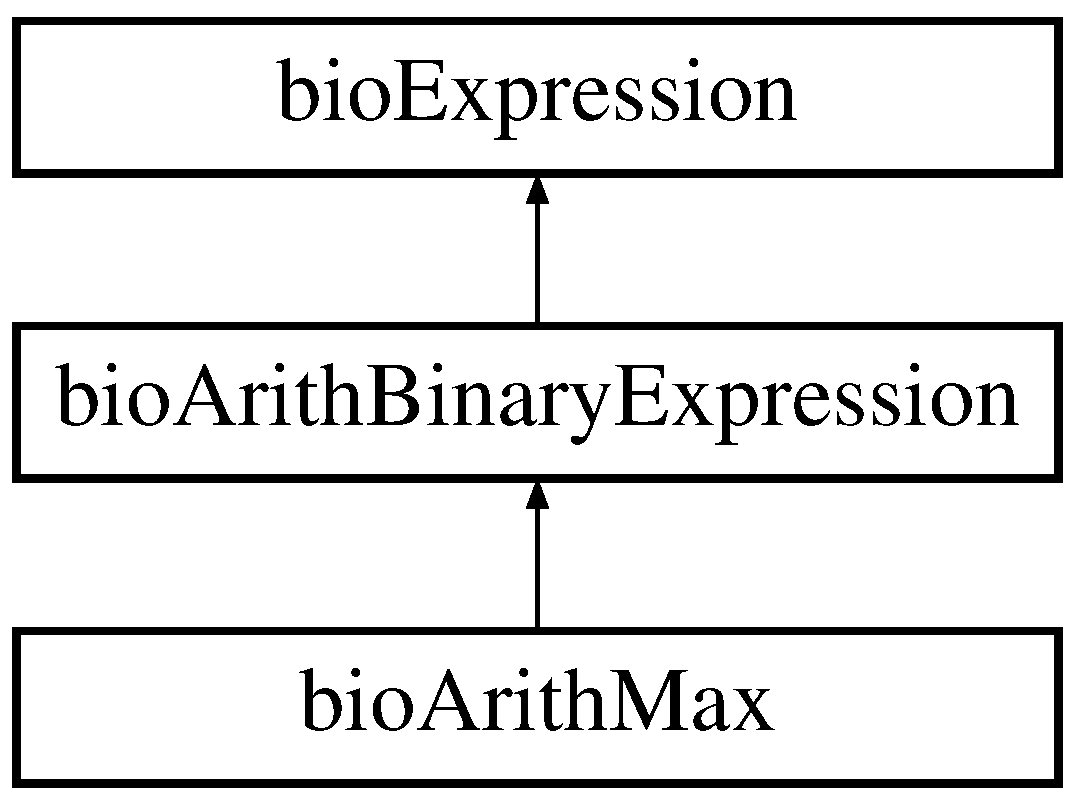
\includegraphics[height=3.000000cm]{classbio_arith_max}
\end{center}
\end{figure}
\subsection*{Public Member Functions}
\begin{DoxyCompactItemize}
\item 
\mbox{\Hypertarget{classbio_arith_max_a095f36a9a9c8d7feb2e9dc687ee80a65}\label{classbio_arith_max_a095f36a9a9c8d7feb2e9dc687ee80a65}} 
{\bfseries bio\+Arith\+Max} (\hyperlink{classbio_expression_repository}{bio\+Expression\+Repository} $\ast$rep, pat\+U\+Long par, pat\+U\+Long left, pat\+U\+Long right, pat\+Error $\ast$\&err)
\item 
virtual pat\+String \hyperlink{classbio_arith_max_a0d4f43812301caafd039e446bbd22bb7}{get\+Operator\+Name} () const
\item 
virtual pat\+Real \hyperlink{classbio_arith_max_a7d8d72eba4b603fadd764cac3cecf23a}{get\+Value} (pat\+Boolean prepare\+Gradient, pat\+U\+Long current\+Lap, pat\+Error $\ast$\&err)
\item 
virtual \hyperlink{classbio_expression}{bio\+Expression} $\ast$ \hyperlink{classbio_arith_max_a4d6fcb906b3140fb4114e36f7a801d22}{get\+Derivative} (pat\+U\+Long a\+Literal\+Id, pat\+Error $\ast$\&err) const
\item 
virtual \hyperlink{classbio_arith_max}{bio\+Arith\+Max} $\ast$ \hyperlink{classbio_arith_max_a3b2838323b5171114cade7522e6f45dc}{get\+Deep\+Copy} (\hyperlink{classbio_expression_repository}{bio\+Expression\+Repository} $\ast$rep, pat\+Error $\ast$\&err) const
\item 
virtual \hyperlink{classbio_arith_max}{bio\+Arith\+Max} $\ast$ \hyperlink{classbio_arith_max_a038037a69623c574752c0e5d56c39e9b}{get\+Shallow\+Copy} (\hyperlink{classbio_expression_repository}{bio\+Expression\+Repository} $\ast$rep, pat\+Error $\ast$\&err) const
\item 
virtual pat\+String \hyperlink{classbio_arith_max_a600790905b0ea5f185b579c630eb25ee}{get\+Expression\+String} () const
\item 
virtual \hyperlink{classbio_function_and_derivatives}{bio\+Function\+And\+Derivatives} $\ast$ \hyperlink{classbio_arith_max_add45318e2ced79172265d99e15214b6c}{get\+Numerical\+Function\+And\+Gradient} (vector$<$ pat\+U\+Long $>$ literal\+Ids, pat\+Boolean compute\+Hessian, pat\+Boolean debug\+Derivatives, pat\+Error $\ast$\&err)
\end{DoxyCompactItemize}
\subsection*{Additional Inherited Members}


\subsection{Detailed Description}
Class implementing a node of the tree representing a max operation 

\subsection{Member Function Documentation}
\mbox{\Hypertarget{classbio_arith_max_a3b2838323b5171114cade7522e6f45dc}\label{classbio_arith_max_a3b2838323b5171114cade7522e6f45dc}} 
\index{bio\+Arith\+Max@{bio\+Arith\+Max}!get\+Deep\+Copy@{get\+Deep\+Copy}}
\index{get\+Deep\+Copy@{get\+Deep\+Copy}!bio\+Arith\+Max@{bio\+Arith\+Max}}
\subsubsection{\texorpdfstring{get\+Deep\+Copy()}{getDeepCopy()}}
{\footnotesize\ttfamily \hyperlink{classbio_arith_max}{bio\+Arith\+Max} $\ast$ bio\+Arith\+Max\+::get\+Deep\+Copy (\begin{DoxyParamCaption}\item[{\hyperlink{classbio_expression_repository}{bio\+Expression\+Repository} $\ast$}]{rep,  }\item[{pat\+Error $\ast$\&}]{err }\end{DoxyParamCaption}) const\hspace{0.3cm}{\ttfamily [virtual]}}

Create a deep copy of the expression and returns a pointer to it. It means that new instances of the children are created. 

Reimplemented from \hyperlink{classbio_expression_a4ee1b8add634078a02eaae26cd40dcc8}{bio\+Expression}.

\mbox{\Hypertarget{classbio_arith_max_a4d6fcb906b3140fb4114e36f7a801d22}\label{classbio_arith_max_a4d6fcb906b3140fb4114e36f7a801d22}} 
\index{bio\+Arith\+Max@{bio\+Arith\+Max}!get\+Derivative@{get\+Derivative}}
\index{get\+Derivative@{get\+Derivative}!bio\+Arith\+Max@{bio\+Arith\+Max}}
\subsubsection{\texorpdfstring{get\+Derivative()}{getDerivative()}}
{\footnotesize\ttfamily \hyperlink{classbio_expression}{bio\+Expression} $\ast$ bio\+Arith\+Max\+::get\+Derivative (\begin{DoxyParamCaption}\item[{pat\+U\+Long}]{a\+Literal\+Id,  }\item[{pat\+Error $\ast$\&}]{err }\end{DoxyParamCaption}) const\hspace{0.3cm}{\ttfamily [virtual]}}

\begin{DoxyReturn}{Returns}
value of the derivative w.\+r.\+t literal 
\end{DoxyReturn}

\begin{DoxyParams}{Parameters}
{\em index} & of the literal involved in the derivative \\
\hline
{\em err} & ref. of the pointer to the error object. \\
\hline
\end{DoxyParams}


Reimplemented from \hyperlink{classbio_expression_a5915579d1193f25f216c1e273c97f2ce}{bio\+Expression}.

\mbox{\Hypertarget{classbio_arith_max_a600790905b0ea5f185b579c630eb25ee}\label{classbio_arith_max_a600790905b0ea5f185b579c630eb25ee}} 
\index{bio\+Arith\+Max@{bio\+Arith\+Max}!get\+Expression\+String@{get\+Expression\+String}}
\index{get\+Expression\+String@{get\+Expression\+String}!bio\+Arith\+Max@{bio\+Arith\+Max}}
\subsubsection{\texorpdfstring{get\+Expression\+String()}{getExpressionString()}}
{\footnotesize\ttfamily pat\+String bio\+Arith\+Max\+::get\+Expression\+String (\begin{DoxyParamCaption}{ }\end{DoxyParamCaption}) const\hspace{0.3cm}{\ttfamily [virtual]}}

Compute a string that represents the expression. It is designed to replace the expression itself when used only for comparison purposes. Code\+: +\{expr1\}\{expr2\}\+: binary plus -\/\{expr1\}\{expr2\}\+: binary minus \{expr1\}\{expr2\}\+: multiplication /\{expr1\}\{expr2\}\+: division $^\wedge$\{expr1\}\{expr2\}\+: power \&\{expr1\}\{expr2\}\+: and $\vert$\{expr1\}\{expr2\}\+: or =\{expr1\}\{expr2\}\+: equal !=\{expr1\}\{expr2\}\+: not equal $<$\{expr1\}\{expr2\}\+: lesser than $<$=\{expr1\}\{expr2\}\+: lesser or equal to $>$\{expr1\}\{expr2\}\+: greater than $>$=\{expr1\}\{expr2\}\+: greater or equal to \$A\{expr\}\+: abs \$D\mbox{[}expr\mbox{]}\mbox{[}\{expr1\}...\{exprN\}\mbox{]}\+: dictionary (\hyperlink{classbio_arith_elem}{bio\+Arith\+Elem}) \$E\{expr\}\+: exp \$L\{expr\}\+: log \$M\{expr\}\+: Unary minus \$\+Piterator\+\_\+name\{expr\}\+: prod \$Q\{string1\}\{string2\}\+: sequence \$\+Siterator\+\_\+name\{expr\}\+: sum \$\+Ziterator\+\_\+name\mbox{[}\{expr1\}...\{exprN\}\mbox{]}\+: merged sum \{expr1\}\{expr2\}...\{exprN\}//\+: list of expressions number\+: constant \#id\+: literal \&id\+: random 

Reimplemented from \hyperlink{classbio_expression_a3e4b4dca58dbbc6f0e411b30eb3f60b4}{bio\+Expression}.

\mbox{\Hypertarget{classbio_arith_max_add45318e2ced79172265d99e15214b6c}\label{classbio_arith_max_add45318e2ced79172265d99e15214b6c}} 
\index{bio\+Arith\+Max@{bio\+Arith\+Max}!get\+Numerical\+Function\+And\+Gradient@{get\+Numerical\+Function\+And\+Gradient}}
\index{get\+Numerical\+Function\+And\+Gradient@{get\+Numerical\+Function\+And\+Gradient}!bio\+Arith\+Max@{bio\+Arith\+Max}}
\subsubsection{\texorpdfstring{get\+Numerical\+Function\+And\+Gradient()}{getNumericalFunctionAndGradient()}}
{\footnotesize\ttfamily \hyperlink{classbio_function_and_derivatives}{bio\+Function\+And\+Derivatives} $\ast$ bio\+Arith\+Max\+::get\+Numerical\+Function\+And\+Gradient (\begin{DoxyParamCaption}\item[{vector$<$ pat\+U\+Long $>$}]{literal\+Ids,  }\item[{pat\+Boolean}]{compute\+Hessian,  }\item[{pat\+Boolean}]{debug\+Derivatives,  }\item[{pat\+Error $\ast$\&}]{err }\end{DoxyParamCaption})\hspace{0.3cm}{\ttfamily [virtual]}}

\begin{DoxyReturn}{Returns}
value and gradient of the expression 
\end{DoxyReturn}

\begin{DoxyParams}{Parameters}
{\em err} & ref. of the pointer to the error object. \\
\hline
\end{DoxyParams}


Reimplemented from \hyperlink{classbio_expression_a91c81ce80c9e972c913b10f5f3c1ed13}{bio\+Expression}.

\mbox{\Hypertarget{classbio_arith_max_a0d4f43812301caafd039e446bbd22bb7}\label{classbio_arith_max_a0d4f43812301caafd039e446bbd22bb7}} 
\index{bio\+Arith\+Max@{bio\+Arith\+Max}!get\+Operator\+Name@{get\+Operator\+Name}}
\index{get\+Operator\+Name@{get\+Operator\+Name}!bio\+Arith\+Max@{bio\+Arith\+Max}}
\subsubsection{\texorpdfstring{get\+Operator\+Name()}{getOperatorName()}}
{\footnotesize\ttfamily pat\+String bio\+Arith\+Max\+::get\+Operator\+Name (\begin{DoxyParamCaption}{ }\end{DoxyParamCaption}) const\hspace{0.3cm}{\ttfamily [virtual]}}

\begin{DoxyReturn}{Returns}
name of the operator 
\end{DoxyReturn}


Reimplemented from \hyperlink{classbio_expression_a2353a4afb3a2b0af7c63aba086a72bde}{bio\+Expression}.

\mbox{\Hypertarget{classbio_arith_max_a038037a69623c574752c0e5d56c39e9b}\label{classbio_arith_max_a038037a69623c574752c0e5d56c39e9b}} 
\index{bio\+Arith\+Max@{bio\+Arith\+Max}!get\+Shallow\+Copy@{get\+Shallow\+Copy}}
\index{get\+Shallow\+Copy@{get\+Shallow\+Copy}!bio\+Arith\+Max@{bio\+Arith\+Max}}
\subsubsection{\texorpdfstring{get\+Shallow\+Copy()}{getShallowCopy()}}
{\footnotesize\ttfamily \hyperlink{classbio_arith_max}{bio\+Arith\+Max} $\ast$ bio\+Arith\+Max\+::get\+Shallow\+Copy (\begin{DoxyParamCaption}\item[{\hyperlink{classbio_expression_repository}{bio\+Expression\+Repository} $\ast$}]{rep,  }\item[{pat\+Error $\ast$\&}]{err }\end{DoxyParamCaption}) const\hspace{0.3cm}{\ttfamily [virtual]}}

Create a shallow copy of the expression and returns a pointer to it. It means that no new instance of the children are created. It is typically called by the repository 

Reimplemented from \hyperlink{classbio_expression_a442534762693b92baaf33928979a1bf8}{bio\+Expression}.

\mbox{\Hypertarget{classbio_arith_max_a7d8d72eba4b603fadd764cac3cecf23a}\label{classbio_arith_max_a7d8d72eba4b603fadd764cac3cecf23a}} 
\index{bio\+Arith\+Max@{bio\+Arith\+Max}!get\+Value@{get\+Value}}
\index{get\+Value@{get\+Value}!bio\+Arith\+Max@{bio\+Arith\+Max}}
\subsubsection{\texorpdfstring{get\+Value()}{getValue()}}
{\footnotesize\ttfamily pat\+Real bio\+Arith\+Max\+::get\+Value (\begin{DoxyParamCaption}\item[{pat\+Boolean}]{prepare\+Gradient,  }\item[{pat\+U\+Long}]{current\+Lap,  }\item[{pat\+Error $\ast$\&}]{err }\end{DoxyParamCaption})\hspace{0.3cm}{\ttfamily [virtual]}}

\begin{DoxyReturn}{Returns}
value of the expression 
\end{DoxyReturn}

\begin{DoxyParams}{Parameters}
{\em err} & ref. of the pointer to the error object. \\
\hline
\end{DoxyParams}


Reimplemented from \hyperlink{classbio_expression_af58662a5d4d456f15bc4f2c9bd4f8a5b}{bio\+Expression}.



The documentation for this class was generated from the following files\+:\begin{DoxyCompactItemize}
\item 
bio\+Arith\+Max.\+h\item 
bio\+Arith\+Max.\+cc\end{DoxyCompactItemize}

\hypertarget{classbio_arith_min}{}\section{bio\+Arith\+Min Class Reference}
\label{classbio_arith_min}\index{bio\+Arith\+Min@{bio\+Arith\+Min}}


{\ttfamily \#include $<$bio\+Arith\+Min.\+h$>$}

Inheritance diagram for bio\+Arith\+Min\+:\begin{figure}[H]
\begin{center}
\leavevmode
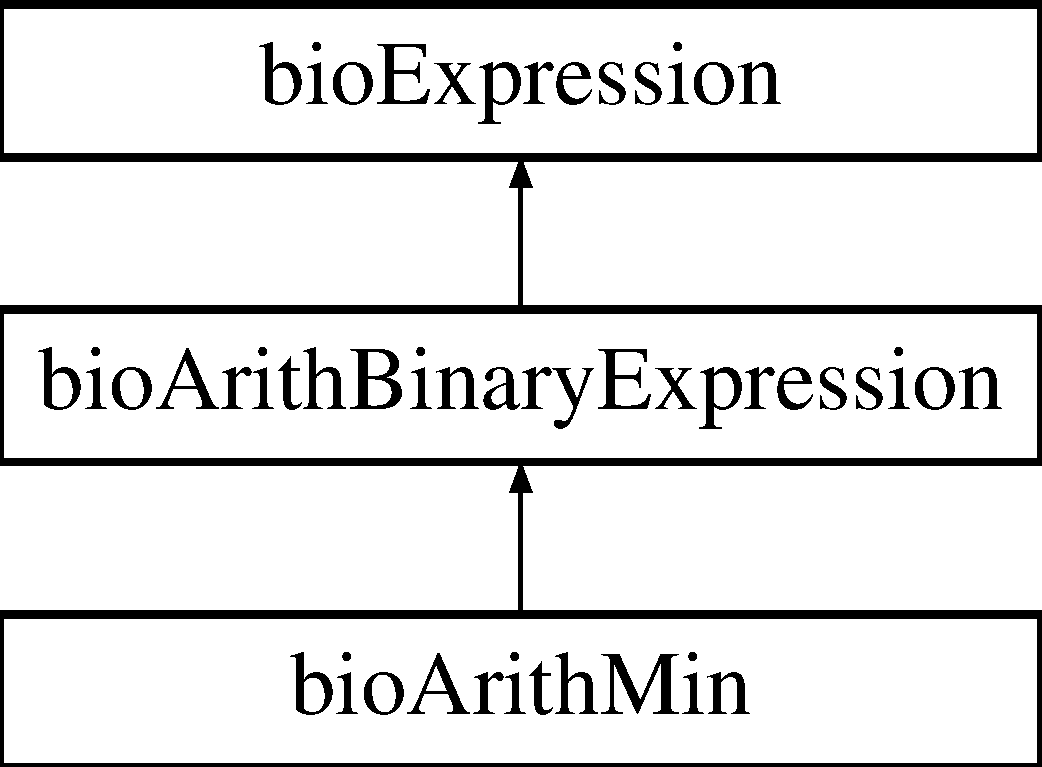
\includegraphics[height=3.000000cm]{classbio_arith_min}
\end{center}
\end{figure}
\subsection*{Public Member Functions}
\begin{DoxyCompactItemize}
\item 
\mbox{\Hypertarget{classbio_arith_min_a8d9b751c23988972cd7523717953e2a8}\label{classbio_arith_min_a8d9b751c23988972cd7523717953e2a8}} 
{\bfseries bio\+Arith\+Min} (\hyperlink{classbio_expression_repository}{bio\+Expression\+Repository} $\ast$rep, pat\+U\+Long par, pat\+U\+Long left, pat\+U\+Long right, pat\+Error $\ast$\&err)
\item 
virtual pat\+String \hyperlink{classbio_arith_min_a09b89bea022328daada894ebdf834e5c}{get\+Operator\+Name} () const
\item 
virtual pat\+Real \hyperlink{classbio_arith_min_a809fd63d92823ab01e0a6af0192c5d2e}{get\+Value} (pat\+Boolean prepare\+Gradient, pat\+U\+Long current\+Lap, pat\+Error $\ast$\&err)
\item 
virtual \hyperlink{classbio_expression}{bio\+Expression} $\ast$ \hyperlink{classbio_arith_min_a385882099c9d71855493b6aa4b6223e1}{get\+Derivative} (pat\+U\+Long a\+Literal\+Id, pat\+Error $\ast$\&err) const
\item 
virtual \hyperlink{classbio_arith_min}{bio\+Arith\+Min} $\ast$ \hyperlink{classbio_arith_min_a2d083461d7be9f1c5abac00fe4066a37}{get\+Deep\+Copy} (\hyperlink{classbio_expression_repository}{bio\+Expression\+Repository} $\ast$rep, pat\+Error $\ast$\&err) const
\item 
virtual \hyperlink{classbio_arith_min}{bio\+Arith\+Min} $\ast$ \hyperlink{classbio_arith_min_a30ded7c95902dd535ba172b2bd4918de}{get\+Shallow\+Copy} (\hyperlink{classbio_expression_repository}{bio\+Expression\+Repository} $\ast$rep, pat\+Error $\ast$\&err) const
\item 
virtual pat\+String \hyperlink{classbio_arith_min_a22f4182d45d18801a763fb1d3d4579a3}{get\+Expression\+String} () const
\item 
virtual \hyperlink{classbio_function_and_derivatives}{bio\+Function\+And\+Derivatives} $\ast$ \hyperlink{classbio_arith_min_aeeb85ace337c2e2f0b8e6a27a698625a}{get\+Numerical\+Function\+And\+Gradient} (vector$<$ pat\+U\+Long $>$ literal\+Ids, pat\+Boolean compute\+Hessian, pat\+Boolean debug\+Derivatives, pat\+Error $\ast$\&err)
\end{DoxyCompactItemize}
\subsection*{Additional Inherited Members}


\subsection{Detailed Description}
Class implementing a node of the tree representing a max operation 

\subsection{Member Function Documentation}
\mbox{\Hypertarget{classbio_arith_min_a2d083461d7be9f1c5abac00fe4066a37}\label{classbio_arith_min_a2d083461d7be9f1c5abac00fe4066a37}} 
\index{bio\+Arith\+Min@{bio\+Arith\+Min}!get\+Deep\+Copy@{get\+Deep\+Copy}}
\index{get\+Deep\+Copy@{get\+Deep\+Copy}!bio\+Arith\+Min@{bio\+Arith\+Min}}
\subsubsection{\texorpdfstring{get\+Deep\+Copy()}{getDeepCopy()}}
{\footnotesize\ttfamily \hyperlink{classbio_arith_min}{bio\+Arith\+Min} $\ast$ bio\+Arith\+Min\+::get\+Deep\+Copy (\begin{DoxyParamCaption}\item[{\hyperlink{classbio_expression_repository}{bio\+Expression\+Repository} $\ast$}]{rep,  }\item[{pat\+Error $\ast$\&}]{err }\end{DoxyParamCaption}) const\hspace{0.3cm}{\ttfamily [virtual]}}

Create a deep copy of the expression and returns a pointer to it. It means that new instances of the children are created. 

Reimplemented from \hyperlink{classbio_expression_a4ee1b8add634078a02eaae26cd40dcc8}{bio\+Expression}.

\mbox{\Hypertarget{classbio_arith_min_a385882099c9d71855493b6aa4b6223e1}\label{classbio_arith_min_a385882099c9d71855493b6aa4b6223e1}} 
\index{bio\+Arith\+Min@{bio\+Arith\+Min}!get\+Derivative@{get\+Derivative}}
\index{get\+Derivative@{get\+Derivative}!bio\+Arith\+Min@{bio\+Arith\+Min}}
\subsubsection{\texorpdfstring{get\+Derivative()}{getDerivative()}}
{\footnotesize\ttfamily \hyperlink{classbio_expression}{bio\+Expression} $\ast$ bio\+Arith\+Min\+::get\+Derivative (\begin{DoxyParamCaption}\item[{pat\+U\+Long}]{a\+Literal\+Id,  }\item[{pat\+Error $\ast$\&}]{err }\end{DoxyParamCaption}) const\hspace{0.3cm}{\ttfamily [virtual]}}

\begin{DoxyReturn}{Returns}
value of the derivative w.\+r.\+t literal 
\end{DoxyReturn}

\begin{DoxyParams}{Parameters}
{\em index} & of the literal involved in the derivative \\
\hline
{\em err} & ref. of the pointer to the error object. \\
\hline
\end{DoxyParams}


Reimplemented from \hyperlink{classbio_expression_a5915579d1193f25f216c1e273c97f2ce}{bio\+Expression}.

\mbox{\Hypertarget{classbio_arith_min_a22f4182d45d18801a763fb1d3d4579a3}\label{classbio_arith_min_a22f4182d45d18801a763fb1d3d4579a3}} 
\index{bio\+Arith\+Min@{bio\+Arith\+Min}!get\+Expression\+String@{get\+Expression\+String}}
\index{get\+Expression\+String@{get\+Expression\+String}!bio\+Arith\+Min@{bio\+Arith\+Min}}
\subsubsection{\texorpdfstring{get\+Expression\+String()}{getExpressionString()}}
{\footnotesize\ttfamily pat\+String bio\+Arith\+Min\+::get\+Expression\+String (\begin{DoxyParamCaption}{ }\end{DoxyParamCaption}) const\hspace{0.3cm}{\ttfamily [virtual]}}

Compute a string that represents the expression. It is designed to replace the expression itself when used only for comparison purposes. Code\+: +\{expr1\}\{expr2\}\+: binary plus -\/\{expr1\}\{expr2\}\+: binary minus \{expr1\}\{expr2\}\+: multiplication /\{expr1\}\{expr2\}\+: division $^\wedge$\{expr1\}\{expr2\}\+: power \&\{expr1\}\{expr2\}\+: and $\vert$\{expr1\}\{expr2\}\+: or =\{expr1\}\{expr2\}\+: equal !=\{expr1\}\{expr2\}\+: not equal $<$\{expr1\}\{expr2\}\+: lesser than $<$=\{expr1\}\{expr2\}\+: lesser or equal to $>$\{expr1\}\{expr2\}\+: greater than $>$=\{expr1\}\{expr2\}\+: greater or equal to \$A\{expr\}\+: abs \$D\mbox{[}expr\mbox{]}\mbox{[}\{expr1\}...\{exprN\}\mbox{]}\+: dictionary (\hyperlink{classbio_arith_elem}{bio\+Arith\+Elem}) \$E\{expr\}\+: exp \$L\{expr\}\+: log \$M\{expr\}\+: Unary minus \$\+Piterator\+\_\+name\{expr\}\+: prod \$Q\{string1\}\{string2\}\+: sequence \$\+Siterator\+\_\+name\{expr\}\+: sum \$\+Ziterator\+\_\+name\mbox{[}\{expr1\}...\{exprN\}\mbox{]}\+: merged sum \{expr1\}\{expr2\}...\{exprN\}//\+: list of expressions number\+: constant \#id\+: literal \&id\+: random 

Reimplemented from \hyperlink{classbio_expression_a3e4b4dca58dbbc6f0e411b30eb3f60b4}{bio\+Expression}.

\mbox{\Hypertarget{classbio_arith_min_aeeb85ace337c2e2f0b8e6a27a698625a}\label{classbio_arith_min_aeeb85ace337c2e2f0b8e6a27a698625a}} 
\index{bio\+Arith\+Min@{bio\+Arith\+Min}!get\+Numerical\+Function\+And\+Gradient@{get\+Numerical\+Function\+And\+Gradient}}
\index{get\+Numerical\+Function\+And\+Gradient@{get\+Numerical\+Function\+And\+Gradient}!bio\+Arith\+Min@{bio\+Arith\+Min}}
\subsubsection{\texorpdfstring{get\+Numerical\+Function\+And\+Gradient()}{getNumericalFunctionAndGradient()}}
{\footnotesize\ttfamily \hyperlink{classbio_function_and_derivatives}{bio\+Function\+And\+Derivatives} $\ast$ bio\+Arith\+Min\+::get\+Numerical\+Function\+And\+Gradient (\begin{DoxyParamCaption}\item[{vector$<$ pat\+U\+Long $>$}]{literal\+Ids,  }\item[{pat\+Boolean}]{compute\+Hessian,  }\item[{pat\+Boolean}]{debug\+Derivatives,  }\item[{pat\+Error $\ast$\&}]{err }\end{DoxyParamCaption})\hspace{0.3cm}{\ttfamily [virtual]}}

\begin{DoxyReturn}{Returns}
value and gradient of the expression 
\end{DoxyReturn}

\begin{DoxyParams}{Parameters}
{\em err} & ref. of the pointer to the error object. \\
\hline
\end{DoxyParams}


Reimplemented from \hyperlink{classbio_expression_a91c81ce80c9e972c913b10f5f3c1ed13}{bio\+Expression}.

\mbox{\Hypertarget{classbio_arith_min_a09b89bea022328daada894ebdf834e5c}\label{classbio_arith_min_a09b89bea022328daada894ebdf834e5c}} 
\index{bio\+Arith\+Min@{bio\+Arith\+Min}!get\+Operator\+Name@{get\+Operator\+Name}}
\index{get\+Operator\+Name@{get\+Operator\+Name}!bio\+Arith\+Min@{bio\+Arith\+Min}}
\subsubsection{\texorpdfstring{get\+Operator\+Name()}{getOperatorName()}}
{\footnotesize\ttfamily pat\+String bio\+Arith\+Min\+::get\+Operator\+Name (\begin{DoxyParamCaption}{ }\end{DoxyParamCaption}) const\hspace{0.3cm}{\ttfamily [virtual]}}

\begin{DoxyReturn}{Returns}
name of the operator 
\end{DoxyReturn}


Reimplemented from \hyperlink{classbio_expression_a2353a4afb3a2b0af7c63aba086a72bde}{bio\+Expression}.

\mbox{\Hypertarget{classbio_arith_min_a30ded7c95902dd535ba172b2bd4918de}\label{classbio_arith_min_a30ded7c95902dd535ba172b2bd4918de}} 
\index{bio\+Arith\+Min@{bio\+Arith\+Min}!get\+Shallow\+Copy@{get\+Shallow\+Copy}}
\index{get\+Shallow\+Copy@{get\+Shallow\+Copy}!bio\+Arith\+Min@{bio\+Arith\+Min}}
\subsubsection{\texorpdfstring{get\+Shallow\+Copy()}{getShallowCopy()}}
{\footnotesize\ttfamily \hyperlink{classbio_arith_min}{bio\+Arith\+Min} $\ast$ bio\+Arith\+Min\+::get\+Shallow\+Copy (\begin{DoxyParamCaption}\item[{\hyperlink{classbio_expression_repository}{bio\+Expression\+Repository} $\ast$}]{rep,  }\item[{pat\+Error $\ast$\&}]{err }\end{DoxyParamCaption}) const\hspace{0.3cm}{\ttfamily [virtual]}}

Create a shallow copy of the expression and returns a pointer to it. It means that no new instance of the children are created. It is typically called by the repository 

Reimplemented from \hyperlink{classbio_expression_a442534762693b92baaf33928979a1bf8}{bio\+Expression}.

\mbox{\Hypertarget{classbio_arith_min_a809fd63d92823ab01e0a6af0192c5d2e}\label{classbio_arith_min_a809fd63d92823ab01e0a6af0192c5d2e}} 
\index{bio\+Arith\+Min@{bio\+Arith\+Min}!get\+Value@{get\+Value}}
\index{get\+Value@{get\+Value}!bio\+Arith\+Min@{bio\+Arith\+Min}}
\subsubsection{\texorpdfstring{get\+Value()}{getValue()}}
{\footnotesize\ttfamily pat\+Real bio\+Arith\+Min\+::get\+Value (\begin{DoxyParamCaption}\item[{pat\+Boolean}]{prepare\+Gradient,  }\item[{pat\+U\+Long}]{current\+Lap,  }\item[{pat\+Error $\ast$\&}]{err }\end{DoxyParamCaption})\hspace{0.3cm}{\ttfamily [virtual]}}

\begin{DoxyReturn}{Returns}
value of the expression 
\end{DoxyReturn}

\begin{DoxyParams}{Parameters}
{\em err} & ref. of the pointer to the error object. \\
\hline
\end{DoxyParams}


Reimplemented from \hyperlink{classbio_expression_af58662a5d4d456f15bc4f2c9bd4f8a5b}{bio\+Expression}.



The documentation for this class was generated from the following files\+:\begin{DoxyCompactItemize}
\item 
bio\+Arith\+Min.\+h\item 
bio\+Arith\+Min.\+cc\end{DoxyCompactItemize}

\hypertarget{classbio_arith_monte_carlo}{}\section{bio\+Arith\+Monte\+Carlo Class Reference}
\label{classbio_arith_monte_carlo}\index{bio\+Arith\+Monte\+Carlo@{bio\+Arith\+Monte\+Carlo}}


{\ttfamily \#include $<$bio\+Arith\+Monte\+Carlo.\+h$>$}

Inheritance diagram for bio\+Arith\+Monte\+Carlo\+:\begin{figure}[H]
\begin{center}
\leavevmode
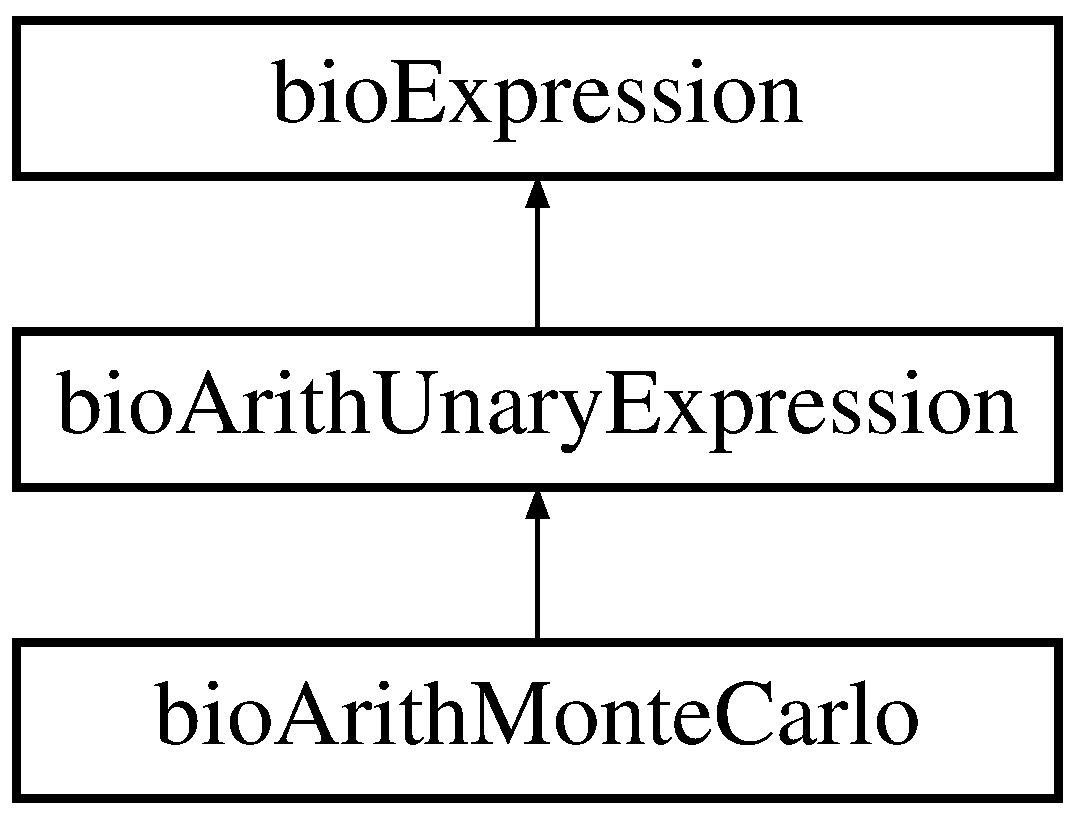
\includegraphics[height=3.000000cm]{classbio_arith_monte_carlo}
\end{center}
\end{figure}
\subsection*{Public Member Functions}
\begin{DoxyCompactItemize}
\item 
\mbox{\Hypertarget{classbio_arith_monte_carlo_a9469254ad5760682005997afdb8ade34}\label{classbio_arith_monte_carlo_a9469254ad5760682005997afdb8ade34}} 
{\bfseries bio\+Arith\+Monte\+Carlo} (\hyperlink{classbio_expression_repository}{bio\+Expression\+Repository} $\ast$rep, pat\+U\+Long par, pat\+U\+Long left, pat\+Error $\ast$\&err)
\item 
\mbox{\Hypertarget{classbio_arith_monte_carlo_a50b9d05e3d17a60468f61e290a765bba}\label{classbio_arith_monte_carlo_a50b9d05e3d17a60468f61e290a765bba}} 
{\bfseries bio\+Arith\+Monte\+Carlo} (\hyperlink{classbio_expression_repository}{bio\+Expression\+Repository} $\ast$rep, pat\+U\+Long par, pat\+U\+Long left, pat\+U\+Long the\+Integrand, pat\+U\+Long the\+Integral, pat\+Error $\ast$\&err)
\item 
\mbox{\Hypertarget{classbio_arith_monte_carlo_a3c813ed84fb565a36c1ef34c176acaa4}\label{classbio_arith_monte_carlo_a3c813ed84fb565a36c1ef34c176acaa4}} 
pat\+Boolean {\bfseries contains\+Monte\+Carlo} () const
\item 
\mbox{\Hypertarget{classbio_arith_monte_carlo_af1f16697ed740b5a94dc39d2fbe8afdc}\label{classbio_arith_monte_carlo_af1f16697ed740b5a94dc39d2fbe8afdc}} 
void {\bfseries check\+Monte\+Carlo} (pat\+Boolean inside\+Monte\+Carlo, pat\+Error $\ast$\&err)
\item 
virtual \hyperlink{classbio_expression}{bio\+Expression} $\ast$ \hyperlink{classbio_arith_monte_carlo_aae0ac80f1c463af6e6d1c3b227bae1e1}{get\+Derivative} (pat\+U\+Long a\+Literal\+Id, pat\+Error $\ast$\&err) const
\item 
virtual pat\+String \hyperlink{classbio_arith_monte_carlo_aa968b16e7b1982445c4aea9aee714d57}{get\+Operator\+Name} () const
\item 
virtual \hyperlink{classbio_arith_monte_carlo}{bio\+Arith\+Monte\+Carlo} $\ast$ \hyperlink{classbio_arith_monte_carlo_a91a8c51e8741c4667d1a61eb738f20f5}{get\+Deep\+Copy} (\hyperlink{classbio_expression_repository}{bio\+Expression\+Repository} $\ast$rep, pat\+Error $\ast$\&err) const
\item 
virtual \hyperlink{classbio_arith_monte_carlo}{bio\+Arith\+Monte\+Carlo} $\ast$ \hyperlink{classbio_arith_monte_carlo_ad91e62a31bbad6cb336f078747fbc7ae}{get\+Shallow\+Copy} (\hyperlink{classbio_expression_repository}{bio\+Expression\+Repository} $\ast$rep, pat\+Error $\ast$\&err) const
\item 
virtual pat\+String \hyperlink{classbio_arith_monte_carlo_ab8753ef1b6b13b97c7991fe238869dbf}{get\+Expression\+String} () const
\item 
virtual pat\+Real \hyperlink{classbio_arith_monte_carlo_a0c1b08214fb40a9b77411c003bd022c5}{get\+Value} (pat\+Boolean prepare\+Gradient, pat\+U\+Long current\+Lap, pat\+Error $\ast$\&err)
\item 
\mbox{\Hypertarget{classbio_arith_monte_carlo_a226b1b342241369bad8ed95c6827a8bb}\label{classbio_arith_monte_carlo_a226b1b342241369bad8ed95c6827a8bb}} 
virtual pat\+U\+Long {\bfseries get\+Number\+Of\+Operations} () const
\item 
virtual \hyperlink{classbio_function_and_derivatives}{bio\+Function\+And\+Derivatives} $\ast$ \hyperlink{classbio_arith_monte_carlo_a6d0d957fe1a3eb664f07bda138d2624a}{get\+Numerical\+Function\+And\+Gradient} (vector$<$ pat\+U\+Long $>$ literal\+Ids, pat\+Boolean compute\+Hessian, pat\+Boolean debug\+Derivatives, pat\+Error $\ast$\&err)
\item 
\mbox{\Hypertarget{classbio_arith_monte_carlo_a33485fa7f36e8ce1e8f8de4edcc5b8de}\label{classbio_arith_monte_carlo_a33485fa7f36e8ce1e8f8de4edcc5b8de}} 
void {\bfseries calculate\+Control\+Variate} (pat\+Error $\ast$\&err)
\item 
\mbox{\Hypertarget{classbio_arith_monte_carlo_a26b6b99bb0bbedb3d7682d717141bdb8}\label{classbio_arith_monte_carlo_a26b6b99bb0bbedb3d7682d717141bdb8}} 
\hyperlink{classbio_function_and_derivatives}{bio\+Function\+And\+Derivatives} $\ast$ {\bfseries get\+Numerical\+Function\+And\+Gradient\+Control\+Variate} (vector$<$ pat\+U\+Long $>$ literal\+Ids, pat\+Boolean compute\+Hessian, pat\+Error $\ast$\&err)
\end{DoxyCompactItemize}
\subsection*{Additional Inherited Members}


\subsection{Detailed Description}
Class implementing a node of the tree representing an integration expression, using Monte Carlo simulation. It is basically a sum over all draws, divided by the number of draws. 

\subsection{Member Function Documentation}
\mbox{\Hypertarget{classbio_arith_monte_carlo_a91a8c51e8741c4667d1a61eb738f20f5}\label{classbio_arith_monte_carlo_a91a8c51e8741c4667d1a61eb738f20f5}} 
\index{bio\+Arith\+Monte\+Carlo@{bio\+Arith\+Monte\+Carlo}!get\+Deep\+Copy@{get\+Deep\+Copy}}
\index{get\+Deep\+Copy@{get\+Deep\+Copy}!bio\+Arith\+Monte\+Carlo@{bio\+Arith\+Monte\+Carlo}}
\subsubsection{\texorpdfstring{get\+Deep\+Copy()}{getDeepCopy()}}
{\footnotesize\ttfamily \hyperlink{classbio_arith_monte_carlo}{bio\+Arith\+Monte\+Carlo} $\ast$ bio\+Arith\+Monte\+Carlo\+::get\+Deep\+Copy (\begin{DoxyParamCaption}\item[{\hyperlink{classbio_expression_repository}{bio\+Expression\+Repository} $\ast$}]{rep,  }\item[{pat\+Error $\ast$\&}]{err }\end{DoxyParamCaption}) const\hspace{0.3cm}{\ttfamily [virtual]}}

Create a deep copy of the expression and returns a pointer to it. It means that new instances of the children are created. 

Reimplemented from \hyperlink{classbio_expression_a4ee1b8add634078a02eaae26cd40dcc8}{bio\+Expression}.

\mbox{\Hypertarget{classbio_arith_monte_carlo_aae0ac80f1c463af6e6d1c3b227bae1e1}\label{classbio_arith_monte_carlo_aae0ac80f1c463af6e6d1c3b227bae1e1}} 
\index{bio\+Arith\+Monte\+Carlo@{bio\+Arith\+Monte\+Carlo}!get\+Derivative@{get\+Derivative}}
\index{get\+Derivative@{get\+Derivative}!bio\+Arith\+Monte\+Carlo@{bio\+Arith\+Monte\+Carlo}}
\subsubsection{\texorpdfstring{get\+Derivative()}{getDerivative()}}
{\footnotesize\ttfamily \hyperlink{classbio_expression}{bio\+Expression} $\ast$ bio\+Arith\+Monte\+Carlo\+::get\+Derivative (\begin{DoxyParamCaption}\item[{pat\+U\+Long}]{a\+Literal\+Id,  }\item[{pat\+Error $\ast$\&}]{err }\end{DoxyParamCaption}) const\hspace{0.3cm}{\ttfamily [virtual]}}

\begin{DoxyReturn}{Returns}
value of the derivative w.\+r.\+t literal 
\end{DoxyReturn}

\begin{DoxyParams}{Parameters}
{\em index} & of the literal involved in the derivative \\
\hline
{\em err} & ref. of the pointer to the error object. \\
\hline
\end{DoxyParams}


Reimplemented from \hyperlink{classbio_expression_a5915579d1193f25f216c1e273c97f2ce}{bio\+Expression}.

\mbox{\Hypertarget{classbio_arith_monte_carlo_ab8753ef1b6b13b97c7991fe238869dbf}\label{classbio_arith_monte_carlo_ab8753ef1b6b13b97c7991fe238869dbf}} 
\index{bio\+Arith\+Monte\+Carlo@{bio\+Arith\+Monte\+Carlo}!get\+Expression\+String@{get\+Expression\+String}}
\index{get\+Expression\+String@{get\+Expression\+String}!bio\+Arith\+Monte\+Carlo@{bio\+Arith\+Monte\+Carlo}}
\subsubsection{\texorpdfstring{get\+Expression\+String()}{getExpressionString()}}
{\footnotesize\ttfamily pat\+String bio\+Arith\+Monte\+Carlo\+::get\+Expression\+String (\begin{DoxyParamCaption}{ }\end{DoxyParamCaption}) const\hspace{0.3cm}{\ttfamily [virtual]}}

Compute a string that represents the expression. It is designed to replace the expression itself when used only for comparison purposes. Code\+: +\{expr1\}\{expr2\}\+: binary plus -\/\{expr1\}\{expr2\}\+: binary minus \{expr1\}\{expr2\}\+: multiplication /\{expr1\}\{expr2\}\+: division $^\wedge$\{expr1\}\{expr2\}\+: power \&\{expr1\}\{expr2\}\+: and $\vert$\{expr1\}\{expr2\}\+: or =\{expr1\}\{expr2\}\+: equal !=\{expr1\}\{expr2\}\+: not equal $<$\{expr1\}\{expr2\}\+: lesser than $<$=\{expr1\}\{expr2\}\+: lesser or equal to $>$\{expr1\}\{expr2\}\+: greater than $>$=\{expr1\}\{expr2\}\+: greater or equal to \$A\{expr\}\+: abs \$D\mbox{[}expr\mbox{]}\mbox{[}\{expr1\}...\{exprN\}\mbox{]}\+: dictionary (\hyperlink{classbio_arith_elem}{bio\+Arith\+Elem}) \$E\{expr\}\+: exp \$L\{expr\}\+: log \$M\{expr\}\+: Unary minus \$\+Piterator\+\_\+name\{expr\}\+: prod \$Q\{string1\}\{string2\}\+: sequence \$\+Siterator\+\_\+name\{expr\}\+: sum \$\+Ziterator\+\_\+name\mbox{[}\{expr1\}...\{exprN\}\mbox{]}\+: merged sum \{expr1\}\{expr2\}...\{exprN\}//\+: list of expressions number\+: constant \#id\+: literal \&id\+: random 

Reimplemented from \hyperlink{classbio_expression_a3e4b4dca58dbbc6f0e411b30eb3f60b4}{bio\+Expression}.

\mbox{\Hypertarget{classbio_arith_monte_carlo_a6d0d957fe1a3eb664f07bda138d2624a}\label{classbio_arith_monte_carlo_a6d0d957fe1a3eb664f07bda138d2624a}} 
\index{bio\+Arith\+Monte\+Carlo@{bio\+Arith\+Monte\+Carlo}!get\+Numerical\+Function\+And\+Gradient@{get\+Numerical\+Function\+And\+Gradient}}
\index{get\+Numerical\+Function\+And\+Gradient@{get\+Numerical\+Function\+And\+Gradient}!bio\+Arith\+Monte\+Carlo@{bio\+Arith\+Monte\+Carlo}}
\subsubsection{\texorpdfstring{get\+Numerical\+Function\+And\+Gradient()}{getNumericalFunctionAndGradient()}}
{\footnotesize\ttfamily \hyperlink{classbio_function_and_derivatives}{bio\+Function\+And\+Derivatives} $\ast$ bio\+Arith\+Monte\+Carlo\+::get\+Numerical\+Function\+And\+Gradient (\begin{DoxyParamCaption}\item[{vector$<$ pat\+U\+Long $>$}]{literal\+Ids,  }\item[{pat\+Boolean}]{compute\+Hessian,  }\item[{pat\+Boolean}]{debug\+Derivatives,  }\item[{pat\+Error $\ast$\&}]{err }\end{DoxyParamCaption})\hspace{0.3cm}{\ttfamily [virtual]}}

\begin{DoxyReturn}{Returns}
value and gradient of the expression 
\end{DoxyReturn}

\begin{DoxyParams}{Parameters}
{\em err} & ref. of the pointer to the error object. \\
\hline
\end{DoxyParams}


Reimplemented from \hyperlink{classbio_expression_a91c81ce80c9e972c913b10f5f3c1ed13}{bio\+Expression}.

\mbox{\Hypertarget{classbio_arith_monte_carlo_aa968b16e7b1982445c4aea9aee714d57}\label{classbio_arith_monte_carlo_aa968b16e7b1982445c4aea9aee714d57}} 
\index{bio\+Arith\+Monte\+Carlo@{bio\+Arith\+Monte\+Carlo}!get\+Operator\+Name@{get\+Operator\+Name}}
\index{get\+Operator\+Name@{get\+Operator\+Name}!bio\+Arith\+Monte\+Carlo@{bio\+Arith\+Monte\+Carlo}}
\subsubsection{\texorpdfstring{get\+Operator\+Name()}{getOperatorName()}}
{\footnotesize\ttfamily pat\+String bio\+Arith\+Monte\+Carlo\+::get\+Operator\+Name (\begin{DoxyParamCaption}{ }\end{DoxyParamCaption}) const\hspace{0.3cm}{\ttfamily [virtual]}}

\begin{DoxyReturn}{Returns}
name of the operator 
\end{DoxyReturn}


Reimplemented from \hyperlink{classbio_expression_a2353a4afb3a2b0af7c63aba086a72bde}{bio\+Expression}.

\mbox{\Hypertarget{classbio_arith_monte_carlo_ad91e62a31bbad6cb336f078747fbc7ae}\label{classbio_arith_monte_carlo_ad91e62a31bbad6cb336f078747fbc7ae}} 
\index{bio\+Arith\+Monte\+Carlo@{bio\+Arith\+Monte\+Carlo}!get\+Shallow\+Copy@{get\+Shallow\+Copy}}
\index{get\+Shallow\+Copy@{get\+Shallow\+Copy}!bio\+Arith\+Monte\+Carlo@{bio\+Arith\+Monte\+Carlo}}
\subsubsection{\texorpdfstring{get\+Shallow\+Copy()}{getShallowCopy()}}
{\footnotesize\ttfamily \hyperlink{classbio_arith_monte_carlo}{bio\+Arith\+Monte\+Carlo} $\ast$ bio\+Arith\+Monte\+Carlo\+::get\+Shallow\+Copy (\begin{DoxyParamCaption}\item[{\hyperlink{classbio_expression_repository}{bio\+Expression\+Repository} $\ast$}]{rep,  }\item[{pat\+Error $\ast$\&}]{err }\end{DoxyParamCaption}) const\hspace{0.3cm}{\ttfamily [virtual]}}

Create a shallow copy of the expression and returns a pointer to it. It means that no new instance of the children are created. It is typically called by the repository 

Reimplemented from \hyperlink{classbio_expression_a442534762693b92baaf33928979a1bf8}{bio\+Expression}.

\mbox{\Hypertarget{classbio_arith_monte_carlo_a0c1b08214fb40a9b77411c003bd022c5}\label{classbio_arith_monte_carlo_a0c1b08214fb40a9b77411c003bd022c5}} 
\index{bio\+Arith\+Monte\+Carlo@{bio\+Arith\+Monte\+Carlo}!get\+Value@{get\+Value}}
\index{get\+Value@{get\+Value}!bio\+Arith\+Monte\+Carlo@{bio\+Arith\+Monte\+Carlo}}
\subsubsection{\texorpdfstring{get\+Value()}{getValue()}}
{\footnotesize\ttfamily pat\+Real bio\+Arith\+Monte\+Carlo\+::get\+Value (\begin{DoxyParamCaption}\item[{pat\+Boolean}]{prepare\+Gradient,  }\item[{pat\+U\+Long}]{current\+Lap,  }\item[{pat\+Error $\ast$\&}]{err }\end{DoxyParamCaption})\hspace{0.3cm}{\ttfamily [virtual]}}

\begin{DoxyReturn}{Returns}
value of the expression 
\end{DoxyReturn}

\begin{DoxyParams}{Parameters}
{\em err} & ref. of the pointer to the error object. \\
\hline
\end{DoxyParams}


Reimplemented from \hyperlink{classbio_expression_af58662a5d4d456f15bc4f2c9bd4f8a5b}{bio\+Expression}.



The documentation for this class was generated from the following files\+:\begin{DoxyCompactItemize}
\item 
bio\+Arith\+Monte\+Carlo.\+h\item 
bio\+Arith\+Monte\+Carlo.\+cc\end{DoxyCompactItemize}

\hypertarget{classbio_arith_mult}{}\section{bio\+Arith\+Mult Class Reference}
\label{classbio_arith_mult}\index{bio\+Arith\+Mult@{bio\+Arith\+Mult}}


{\ttfamily \#include $<$bio\+Arith\+Mult.\+h$>$}

Inheritance diagram for bio\+Arith\+Mult\+:\begin{figure}[H]
\begin{center}
\leavevmode
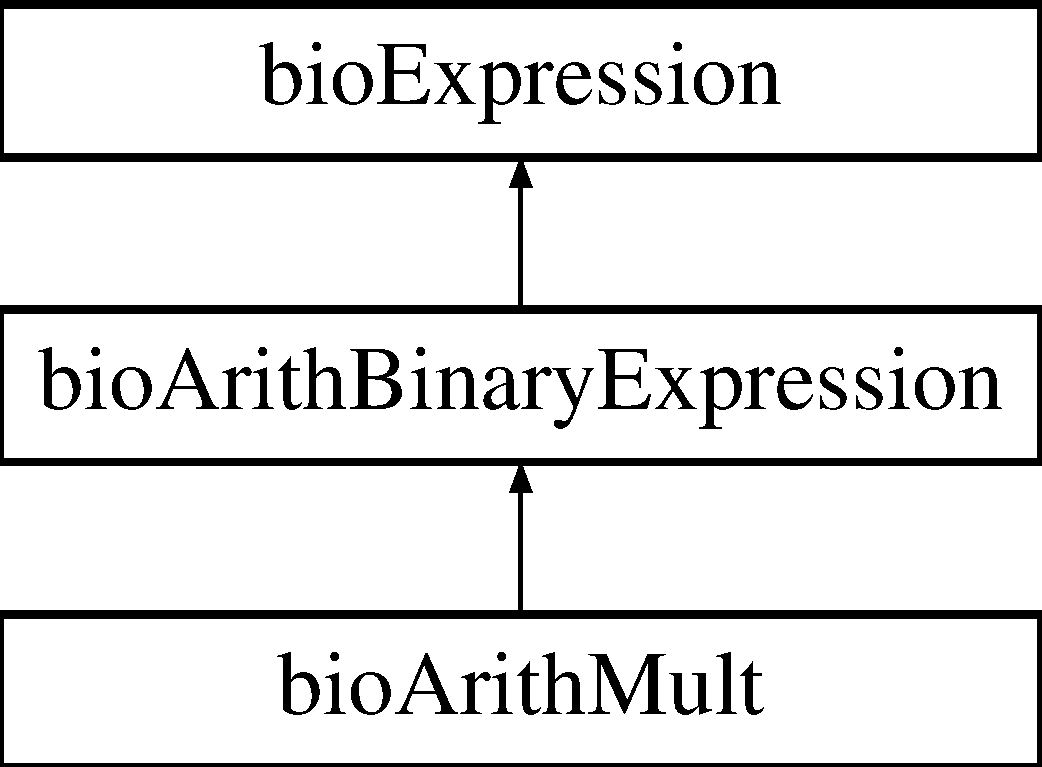
\includegraphics[height=3.000000cm]{classbio_arith_mult}
\end{center}
\end{figure}
\subsection*{Public Member Functions}
\begin{DoxyCompactItemize}
\item 
\mbox{\Hypertarget{classbio_arith_mult_ac3da725646bfbd4e8de4332e2d06445e}\label{classbio_arith_mult_ac3da725646bfbd4e8de4332e2d06445e}} 
{\bfseries bio\+Arith\+Mult} (\hyperlink{classbio_expression_repository}{bio\+Expression\+Repository} $\ast$rep, pat\+U\+Long par, pat\+U\+Long left, pat\+U\+Long right, pat\+Error $\ast$\&err)
\item 
virtual pat\+String \hyperlink{classbio_arith_mult_aff182437fd5a1259cbc79fc7f8bc4956}{get\+Operator\+Name} () const
\item 
virtual pat\+Real \hyperlink{classbio_arith_mult_a5f0d4c6fe299be5b88cbcab100def6c9}{get\+Value} (pat\+Boolean prepare\+Gradient, pat\+U\+Long current\+Lap, pat\+Error $\ast$\&err)
\item 
virtual \hyperlink{classbio_expression}{bio\+Expression} $\ast$ \hyperlink{classbio_arith_mult_a77183d650695b163328878a88fcb02a7}{get\+Derivative} (pat\+U\+Long a\+Literal, pat\+Error $\ast$\&err) const
\item 
virtual \hyperlink{classbio_arith_mult}{bio\+Arith\+Mult} $\ast$ \hyperlink{classbio_arith_mult_a1b6b5a5ce5e104bf5a69010ad67ecd11}{get\+Deep\+Copy} (\hyperlink{classbio_expression_repository}{bio\+Expression\+Repository} $\ast$rep, pat\+Error $\ast$\&err) const
\item 
virtual \hyperlink{classbio_arith_mult}{bio\+Arith\+Mult} $\ast$ \hyperlink{classbio_arith_mult_a58d1f8dec3f450d17bbdfe4f98b18c19}{get\+Shallow\+Copy} (\hyperlink{classbio_expression_repository}{bio\+Expression\+Repository} $\ast$rep, pat\+Error $\ast$\&err) const
\item 
virtual pat\+Boolean \hyperlink{classbio_arith_mult_aedfa0cf623dde749da1760ad7fd9e326}{is\+Structurally\+Zero} () const
\item 
virtual pat\+String \hyperlink{classbio_arith_mult_a7a19012c1cfe783b75de9a9c961587c2}{get\+Expression\+String} () const
\item 
virtual \hyperlink{classbio_function_and_derivatives}{bio\+Function\+And\+Derivatives} $\ast$ \hyperlink{classbio_arith_mult_a18612adf78adad46a0a19f2a57c4b32d}{get\+Numerical\+Function\+And\+Gradient} (vector$<$ pat\+U\+Long $>$ literal\+Ids, pat\+Boolean compute\+Hessian, pat\+Boolean debug\+Derivatives, pat\+Error $\ast$\&err)
\end{DoxyCompactItemize}
\subsection*{Additional Inherited Members}


\subsection{Detailed Description}
Class implementing a node for a multiplication operation 

\subsection{Member Function Documentation}
\mbox{\Hypertarget{classbio_arith_mult_a1b6b5a5ce5e104bf5a69010ad67ecd11}\label{classbio_arith_mult_a1b6b5a5ce5e104bf5a69010ad67ecd11}} 
\index{bio\+Arith\+Mult@{bio\+Arith\+Mult}!get\+Deep\+Copy@{get\+Deep\+Copy}}
\index{get\+Deep\+Copy@{get\+Deep\+Copy}!bio\+Arith\+Mult@{bio\+Arith\+Mult}}
\subsubsection{\texorpdfstring{get\+Deep\+Copy()}{getDeepCopy()}}
{\footnotesize\ttfamily \hyperlink{classbio_arith_mult}{bio\+Arith\+Mult} $\ast$ bio\+Arith\+Mult\+::get\+Deep\+Copy (\begin{DoxyParamCaption}\item[{\hyperlink{classbio_expression_repository}{bio\+Expression\+Repository} $\ast$}]{rep,  }\item[{pat\+Error $\ast$\&}]{err }\end{DoxyParamCaption}) const\hspace{0.3cm}{\ttfamily [virtual]}}

Create a deep copy of the expression and returns a pointer to it. It means that new instances of the children are created. 

Reimplemented from \hyperlink{classbio_expression_a4ee1b8add634078a02eaae26cd40dcc8}{bio\+Expression}.

\mbox{\Hypertarget{classbio_arith_mult_a77183d650695b163328878a88fcb02a7}\label{classbio_arith_mult_a77183d650695b163328878a88fcb02a7}} 
\index{bio\+Arith\+Mult@{bio\+Arith\+Mult}!get\+Derivative@{get\+Derivative}}
\index{get\+Derivative@{get\+Derivative}!bio\+Arith\+Mult@{bio\+Arith\+Mult}}
\subsubsection{\texorpdfstring{get\+Derivative()}{getDerivative()}}
{\footnotesize\ttfamily \hyperlink{classbio_expression}{bio\+Expression} $\ast$ bio\+Arith\+Mult\+::get\+Derivative (\begin{DoxyParamCaption}\item[{pat\+U\+Long}]{a\+Literal\+Id,  }\item[{pat\+Error $\ast$\&}]{err }\end{DoxyParamCaption}) const\hspace{0.3cm}{\ttfamily [virtual]}}

\begin{DoxyReturn}{Returns}
value of the derivative w.\+r.\+t literal 
\end{DoxyReturn}

\begin{DoxyParams}{Parameters}
{\em index} & of the literal involved in the derivative \\
\hline
{\em err} & ref. of the pointer to the error object. \\
\hline
\end{DoxyParams}


Reimplemented from \hyperlink{classbio_expression_a5915579d1193f25f216c1e273c97f2ce}{bio\+Expression}.

\mbox{\Hypertarget{classbio_arith_mult_a7a19012c1cfe783b75de9a9c961587c2}\label{classbio_arith_mult_a7a19012c1cfe783b75de9a9c961587c2}} 
\index{bio\+Arith\+Mult@{bio\+Arith\+Mult}!get\+Expression\+String@{get\+Expression\+String}}
\index{get\+Expression\+String@{get\+Expression\+String}!bio\+Arith\+Mult@{bio\+Arith\+Mult}}
\subsubsection{\texorpdfstring{get\+Expression\+String()}{getExpressionString()}}
{\footnotesize\ttfamily pat\+String bio\+Arith\+Mult\+::get\+Expression\+String (\begin{DoxyParamCaption}{ }\end{DoxyParamCaption}) const\hspace{0.3cm}{\ttfamily [virtual]}}

Compute a string that represents the expression. It is designed to replace the expression itself when used only for comparison purposes. Code\+: +\{expr1\}\{expr2\}\+: binary plus -\/\{expr1\}\{expr2\}\+: binary minus \{expr1\}\{expr2\}\+: multiplication /\{expr1\}\{expr2\}\+: division $^\wedge$\{expr1\}\{expr2\}\+: power \&\{expr1\}\{expr2\}\+: and $\vert$\{expr1\}\{expr2\}\+: or =\{expr1\}\{expr2\}\+: equal !=\{expr1\}\{expr2\}\+: not equal $<$\{expr1\}\{expr2\}\+: lesser than $<$=\{expr1\}\{expr2\}\+: lesser or equal to $>$\{expr1\}\{expr2\}\+: greater than $>$=\{expr1\}\{expr2\}\+: greater or equal to \$A\{expr\}\+: abs \$D\mbox{[}expr\mbox{]}\mbox{[}\{expr1\}...\{exprN\}\mbox{]}\+: dictionary (\hyperlink{classbio_arith_elem}{bio\+Arith\+Elem}) \$E\{expr\}\+: exp \$L\{expr\}\+: log \$M\{expr\}\+: Unary minus \$\+Piterator\+\_\+name\{expr\}\+: prod \$Q\{string1\}\{string2\}\+: sequence \$\+Siterator\+\_\+name\{expr\}\+: sum \$\+Ziterator\+\_\+name\mbox{[}\{expr1\}...\{exprN\}\mbox{]}\+: merged sum \{expr1\}\{expr2\}...\{exprN\}//\+: list of expressions number\+: constant \#id\+: literal \&id\+: random 

Reimplemented from \hyperlink{classbio_expression_a3e4b4dca58dbbc6f0e411b30eb3f60b4}{bio\+Expression}.

\mbox{\Hypertarget{classbio_arith_mult_a18612adf78adad46a0a19f2a57c4b32d}\label{classbio_arith_mult_a18612adf78adad46a0a19f2a57c4b32d}} 
\index{bio\+Arith\+Mult@{bio\+Arith\+Mult}!get\+Numerical\+Function\+And\+Gradient@{get\+Numerical\+Function\+And\+Gradient}}
\index{get\+Numerical\+Function\+And\+Gradient@{get\+Numerical\+Function\+And\+Gradient}!bio\+Arith\+Mult@{bio\+Arith\+Mult}}
\subsubsection{\texorpdfstring{get\+Numerical\+Function\+And\+Gradient()}{getNumericalFunctionAndGradient()}}
{\footnotesize\ttfamily \hyperlink{classbio_function_and_derivatives}{bio\+Function\+And\+Derivatives} $\ast$ bio\+Arith\+Mult\+::get\+Numerical\+Function\+And\+Gradient (\begin{DoxyParamCaption}\item[{vector$<$ pat\+U\+Long $>$}]{literal\+Ids,  }\item[{pat\+Boolean}]{compute\+Hessian,  }\item[{pat\+Boolean}]{debug\+Derivatives,  }\item[{pat\+Error $\ast$\&}]{err }\end{DoxyParamCaption})\hspace{0.3cm}{\ttfamily [virtual]}}

\begin{DoxyReturn}{Returns}
value and gradient of the expression 
\end{DoxyReturn}

\begin{DoxyParams}{Parameters}
{\em err} & ref. of the pointer to the error object. \\
\hline
\end{DoxyParams}


Reimplemented from \hyperlink{classbio_expression_a91c81ce80c9e972c913b10f5f3c1ed13}{bio\+Expression}.

\mbox{\Hypertarget{classbio_arith_mult_aff182437fd5a1259cbc79fc7f8bc4956}\label{classbio_arith_mult_aff182437fd5a1259cbc79fc7f8bc4956}} 
\index{bio\+Arith\+Mult@{bio\+Arith\+Mult}!get\+Operator\+Name@{get\+Operator\+Name}}
\index{get\+Operator\+Name@{get\+Operator\+Name}!bio\+Arith\+Mult@{bio\+Arith\+Mult}}
\subsubsection{\texorpdfstring{get\+Operator\+Name()}{getOperatorName()}}
{\footnotesize\ttfamily pat\+String bio\+Arith\+Mult\+::get\+Operator\+Name (\begin{DoxyParamCaption}{ }\end{DoxyParamCaption}) const\hspace{0.3cm}{\ttfamily [virtual]}}

\begin{DoxyReturn}{Returns}
name of the operator 
\end{DoxyReturn}


Reimplemented from \hyperlink{classbio_expression_a2353a4afb3a2b0af7c63aba086a72bde}{bio\+Expression}.

\mbox{\Hypertarget{classbio_arith_mult_a58d1f8dec3f450d17bbdfe4f98b18c19}\label{classbio_arith_mult_a58d1f8dec3f450d17bbdfe4f98b18c19}} 
\index{bio\+Arith\+Mult@{bio\+Arith\+Mult}!get\+Shallow\+Copy@{get\+Shallow\+Copy}}
\index{get\+Shallow\+Copy@{get\+Shallow\+Copy}!bio\+Arith\+Mult@{bio\+Arith\+Mult}}
\subsubsection{\texorpdfstring{get\+Shallow\+Copy()}{getShallowCopy()}}
{\footnotesize\ttfamily \hyperlink{classbio_arith_mult}{bio\+Arith\+Mult} $\ast$ bio\+Arith\+Mult\+::get\+Shallow\+Copy (\begin{DoxyParamCaption}\item[{\hyperlink{classbio_expression_repository}{bio\+Expression\+Repository} $\ast$}]{rep,  }\item[{pat\+Error $\ast$\&}]{err }\end{DoxyParamCaption}) const\hspace{0.3cm}{\ttfamily [virtual]}}

Create a shallow copy of the expression and returns a pointer to it. It means that no new instance of the children are created. It is typically called by the repository 

Reimplemented from \hyperlink{classbio_expression_a442534762693b92baaf33928979a1bf8}{bio\+Expression}.

\mbox{\Hypertarget{classbio_arith_mult_a5f0d4c6fe299be5b88cbcab100def6c9}\label{classbio_arith_mult_a5f0d4c6fe299be5b88cbcab100def6c9}} 
\index{bio\+Arith\+Mult@{bio\+Arith\+Mult}!get\+Value@{get\+Value}}
\index{get\+Value@{get\+Value}!bio\+Arith\+Mult@{bio\+Arith\+Mult}}
\subsubsection{\texorpdfstring{get\+Value()}{getValue()}}
{\footnotesize\ttfamily pat\+Real bio\+Arith\+Mult\+::get\+Value (\begin{DoxyParamCaption}\item[{pat\+Boolean}]{prepare\+Gradient,  }\item[{pat\+U\+Long}]{current\+Lap,  }\item[{pat\+Error $\ast$\&}]{err }\end{DoxyParamCaption})\hspace{0.3cm}{\ttfamily [virtual]}}

\begin{DoxyReturn}{Returns}
value of the expression 
\end{DoxyReturn}

\begin{DoxyParams}{Parameters}
{\em err} & ref. of the pointer to the error object. \\
\hline
\end{DoxyParams}


Reimplemented from \hyperlink{classbio_expression_af58662a5d4d456f15bc4f2c9bd4f8a5b}{bio\+Expression}.

\mbox{\Hypertarget{classbio_arith_mult_aedfa0cf623dde749da1760ad7fd9e326}\label{classbio_arith_mult_aedfa0cf623dde749da1760ad7fd9e326}} 
\index{bio\+Arith\+Mult@{bio\+Arith\+Mult}!is\+Structurally\+Zero@{is\+Structurally\+Zero}}
\index{is\+Structurally\+Zero@{is\+Structurally\+Zero}!bio\+Arith\+Mult@{bio\+Arith\+Mult}}
\subsubsection{\texorpdfstring{is\+Structurally\+Zero()}{isStructurallyZero()}}
{\footnotesize\ttfamily pat\+Boolean bio\+Arith\+Mult\+::is\+Structurally\+Zero (\begin{DoxyParamCaption}{ }\end{DoxyParamCaption}) const\hspace{0.3cm}{\ttfamily [virtual]}}

return pat\+T\+R\+UE if the expression is structurally 0 so that there is no need to evaluate it. In the base class, it return pat\+F\+A\+L\+SE. 

Reimplemented from \hyperlink{classbio_expression_a264c6d78671610ada8261d698e4c4c42}{bio\+Expression}.



The documentation for this class was generated from the following files\+:\begin{DoxyCompactItemize}
\item 
bio\+Arith\+Mult.\+h\item 
bio\+Arith\+Mult.\+cc\end{DoxyCompactItemize}

\hypertarget{classbio_arith_multinary_expression}{}\section{bio\+Arith\+Multinary\+Expression Class Reference}
\label{classbio_arith_multinary_expression}\index{bio\+Arith\+Multinary\+Expression@{bio\+Arith\+Multinary\+Expression}}


{\ttfamily \#include $<$bio\+Arith\+Multinary\+Expression.\+h$>$}

Inheritance diagram for bio\+Arith\+Multinary\+Expression\+:\begin{figure}[H]
\begin{center}
\leavevmode
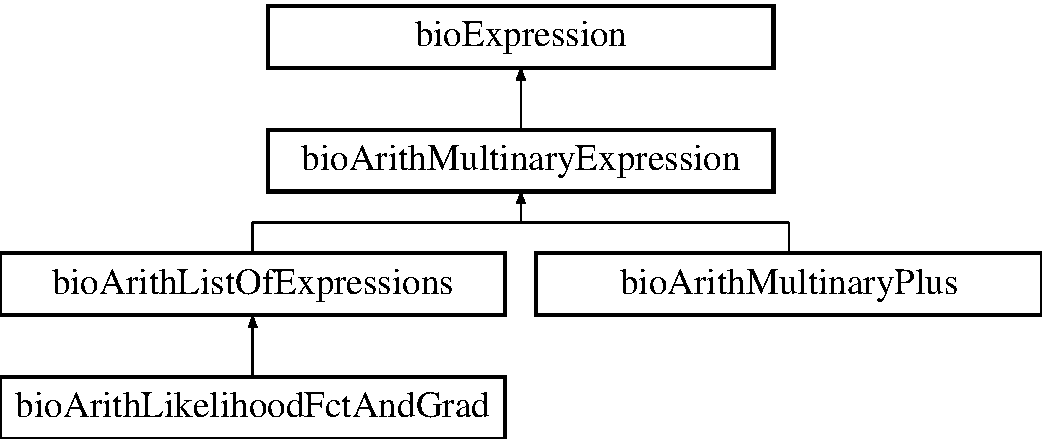
\includegraphics[height=4.000000cm]{classbio_arith_multinary_expression}
\end{center}
\end{figure}
\subsection*{Public Member Functions}
\begin{DoxyCompactItemize}
\item 
\mbox{\Hypertarget{classbio_arith_multinary_expression_a2aa44d4013d63760b590225228d41fe7}\label{classbio_arith_multinary_expression_a2aa44d4013d63760b590225228d41fe7}} 
{\bfseries bio\+Arith\+Multinary\+Expression} (\hyperlink{classbio_expression_repository}{bio\+Expression\+Repository} $\ast$rep, pat\+U\+Long par, vector$<$ pat\+U\+Long $>$ l, pat\+Error $\ast$\&err)
\item 
\mbox{\Hypertarget{classbio_arith_multinary_expression_a91153f21a2aee1804944a2c9fda23f76}\label{classbio_arith_multinary_expression_a91153f21a2aee1804944a2c9fda23f76}} 
virtual vector$<$ pat\+U\+Long $>$ {\bfseries get\+Children\+Ids} () const
\item 
\mbox{\Hypertarget{classbio_arith_multinary_expression_a5cc2ce0bb83b7458e49efbe71bc6f617}\label{classbio_arith_multinary_expression_a5cc2ce0bb83b7458e49efbe71bc6f617}} 
virtual \hyperlink{classbio_expression}{bio\+Expression} $\ast$ {\bfseries get\+Child} (pat\+U\+Long index, pat\+Error $\ast$\&err) const
\item 
virtual pat\+String \hyperlink{classbio_arith_multinary_expression_a769ab218dc1f1efcdaf3204da0ecc705}{get\+Expression} (pat\+Error $\ast$\&err) const
\item 
\mbox{\Hypertarget{classbio_arith_multinary_expression_af08df3df6ae0c84459b741649dc604bd}\label{classbio_arith_multinary_expression_af08df3df6ae0c84459b741649dc604bd}} 
virtual pat\+U\+Long {\bfseries get\+Number\+Of\+Operations} () const
\item 
\mbox{\Hypertarget{classbio_arith_multinary_expression_a8bcf2022391ab3a356623c63047a52b9}\label{classbio_arith_multinary_expression_a8bcf2022391ab3a356623c63047a52b9}} 
virtual pat\+Boolean {\bfseries depends\+Of} (pat\+U\+Long a\+Literal\+Id) const
\item 
\mbox{\Hypertarget{classbio_arith_multinary_expression_afb4941e95c5957c5f666a0e84b030721}\label{classbio_arith_multinary_expression_afb4941e95c5957c5f666a0e84b030721}} 
virtual pat\+Boolean {\bfseries contains\+An\+Iterator} () const
\item 
\mbox{\Hypertarget{classbio_arith_multinary_expression_ac78de0c49d0e1d78403ef49462ee9e62}\label{classbio_arith_multinary_expression_ac78de0c49d0e1d78403ef49462ee9e62}} 
virtual pat\+Boolean {\bfseries contains\+An\+Iterator\+On\+Rows} () const
\item 
\mbox{\Hypertarget{classbio_arith_multinary_expression_a11268a13685f7d66c2362ce5c8b4468b}\label{classbio_arith_multinary_expression_a11268a13685f7d66c2362ce5c8b4468b}} 
virtual pat\+Boolean {\bfseries contains\+An\+Integral} () const
\item 
\mbox{\Hypertarget{classbio_arith_multinary_expression_a51de24ca079fccb0ca51e40ba707e908}\label{classbio_arith_multinary_expression_a51de24ca079fccb0ca51e40ba707e908}} 
virtual pat\+Boolean {\bfseries contains\+A\+Sequence} () const
\item 
\mbox{\Hypertarget{classbio_arith_multinary_expression_af846c5bbae18e41de5d8ce9dcd7a549f}\label{classbio_arith_multinary_expression_af846c5bbae18e41de5d8ce9dcd7a549f}} 
virtual void {\bfseries simplify\+Zeros} (pat\+Error $\ast$\&err)
\item 
\mbox{\Hypertarget{classbio_arith_multinary_expression_a33798f6bf71d8bdfc17b4220195218be}\label{classbio_arith_multinary_expression_a33798f6bf71d8bdfc17b4220195218be}} 
virtual void {\bfseries collect\+Expression\+Ids} (set$<$ pat\+U\+Long $>$ $\ast$s) const
\item 
\mbox{\Hypertarget{classbio_arith_multinary_expression_af09caa161b5988194efc389e7ed3f199}\label{classbio_arith_multinary_expression_af09caa161b5988194efc389e7ed3f199}} 
virtual pat\+String {\bfseries check} (pat\+Error $\ast$\&err) const
\end{DoxyCompactItemize}
\subsection*{Protected Attributes}
\begin{DoxyCompactItemize}
\item 
\mbox{\Hypertarget{classbio_arith_multinary_expression_af2eb40560537ea5d77d5c4a137195f6c}\label{classbio_arith_multinary_expression_af2eb40560537ea5d77d5c4a137195f6c}} 
vector$<$ \hyperlink{classbio_expression}{bio\+Expression} $\ast$ $>$ {\bfseries list\+Of\+Children}
\item 
\mbox{\Hypertarget{classbio_arith_multinary_expression_ae0410053810d53bee59471478d9b3add}\label{classbio_arith_multinary_expression_ae0410053810d53bee59471478d9b3add}} 
vector$<$ pat\+U\+Long $>$ {\bfseries list\+Of\+Children\+Ids}
\end{DoxyCompactItemize}


\subsection{Detailed Description}
Abstract class for a multinary expressions 

\subsection{Member Function Documentation}
\mbox{\Hypertarget{classbio_arith_multinary_expression_a769ab218dc1f1efcdaf3204da0ecc705}\label{classbio_arith_multinary_expression_a769ab218dc1f1efcdaf3204da0ecc705}} 
\index{bio\+Arith\+Multinary\+Expression@{bio\+Arith\+Multinary\+Expression}!get\+Expression@{get\+Expression}}
\index{get\+Expression@{get\+Expression}!bio\+Arith\+Multinary\+Expression@{bio\+Arith\+Multinary\+Expression}}
\subsubsection{\texorpdfstring{get\+Expression()}{getExpression()}}
{\footnotesize\ttfamily pat\+String bio\+Arith\+Multinary\+Expression\+::get\+Expression (\begin{DoxyParamCaption}\item[{pat\+Error $\ast$\&}]{err }\end{DoxyParamCaption}) const\hspace{0.3cm}{\ttfamily [virtual]}}

\begin{DoxyReturn}{Returns}
printed expression 
\end{DoxyReturn}


Reimplemented from \hyperlink{classbio_expression_a66a83eb0caac18dd5e568ffde5a8b5d4}{bio\+Expression}.



Reimplemented in \hyperlink{classbio_arith_multinary_plus_a11b1c8e85618101f78dee811b2bf2630}{bio\+Arith\+Multinary\+Plus}, and \hyperlink{classbio_arith_likelihood_fct_and_grad_ae264b073115dcff703cf2b7926384976}{bio\+Arith\+Likelihood\+Fct\+And\+Grad}.



The documentation for this class was generated from the following files\+:\begin{DoxyCompactItemize}
\item 
bio\+Arith\+Multinary\+Expression.\+h\item 
bio\+Arith\+Multinary\+Expression.\+cc\end{DoxyCompactItemize}

\hypertarget{classbio_arith_multinary_plus}{}\section{bio\+Arith\+Multinary\+Plus Class Reference}
\label{classbio_arith_multinary_plus}\index{bio\+Arith\+Multinary\+Plus@{bio\+Arith\+Multinary\+Plus}}


{\ttfamily \#include $<$bio\+Arith\+Multinary\+Plus.\+h$>$}

Inheritance diagram for bio\+Arith\+Multinary\+Plus\+:\begin{figure}[H]
\begin{center}
\leavevmode
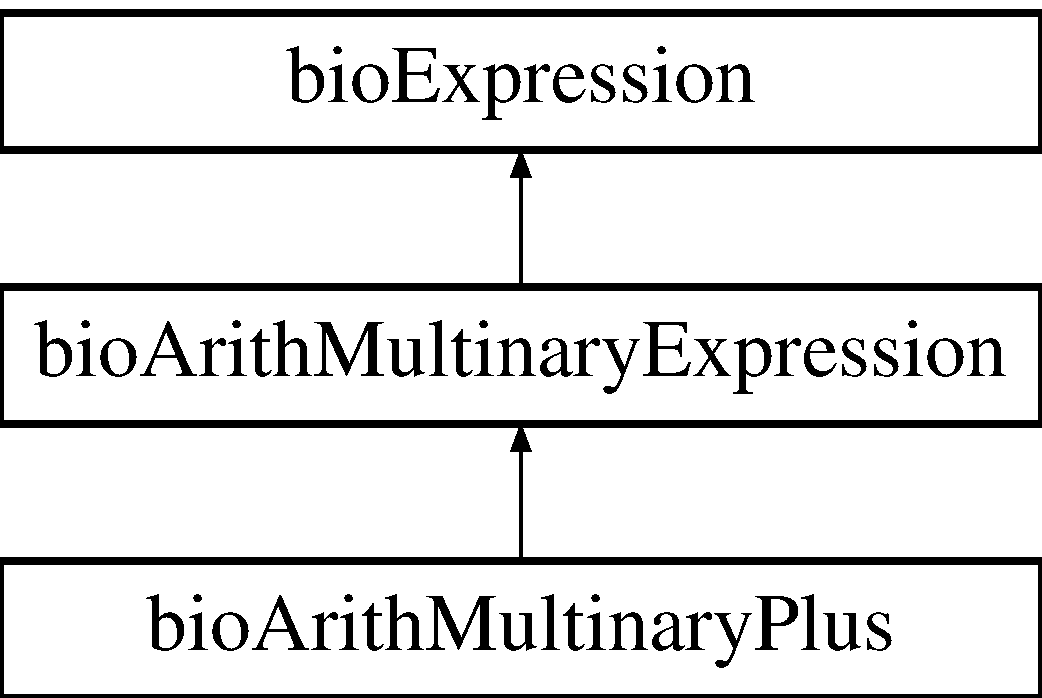
\includegraphics[height=3.000000cm]{classbio_arith_multinary_plus}
\end{center}
\end{figure}
\subsection*{Public Member Functions}
\begin{DoxyCompactItemize}
\item 
\mbox{\Hypertarget{classbio_arith_multinary_plus_a7f0c283c8ce8b96d3cc8e023e192b108}\label{classbio_arith_multinary_plus_a7f0c283c8ce8b96d3cc8e023e192b108}} 
{\bfseries bio\+Arith\+Multinary\+Plus} (\hyperlink{classbio_expression_repository}{bio\+Expression\+Repository} $\ast$rep, pat\+U\+Long par, vector$<$ pat\+U\+Long $>$ l, pat\+Error $\ast$\&err)
\item 
virtual pat\+String \hyperlink{classbio_arith_multinary_plus_ac43848551e8c792e9776b7a5e8aef51b}{get\+Operator\+Name} () const
\item 
virtual pat\+Real \hyperlink{classbio_arith_multinary_plus_a90c1c66054e19f52a4424664f7c09d7a}{get\+Value} (pat\+Boolean prepare\+Gradient, pat\+U\+Long current\+Lap, pat\+Error $\ast$\&err)
\item 
virtual \hyperlink{classbio_expression}{bio\+Expression} $\ast$ \hyperlink{classbio_arith_multinary_plus_a6677355df11e314a1729fb7bd79d9188}{get\+Derivative} (pat\+U\+Long a\+Literal\+Id, pat\+Error $\ast$\&err) const
\item 
virtual \hyperlink{classbio_arith_multinary_plus}{bio\+Arith\+Multinary\+Plus} $\ast$ \hyperlink{classbio_arith_multinary_plus_acdd35f59addcdc2e2947fe0d3f594e1f}{get\+Deep\+Copy} (\hyperlink{classbio_expression_repository}{bio\+Expression\+Repository} $\ast$rep, pat\+Error $\ast$\&err) const
\item 
virtual \hyperlink{classbio_arith_multinary_plus}{bio\+Arith\+Multinary\+Plus} $\ast$ \hyperlink{classbio_arith_multinary_plus_a026a46872ed07e51b2a337f45b5086ad}{get\+Shallow\+Copy} (\hyperlink{classbio_expression_repository}{bio\+Expression\+Repository} $\ast$rep, pat\+Error $\ast$\&err) const
\item 
virtual pat\+String \hyperlink{classbio_arith_multinary_plus_a11b1c8e85618101f78dee811b2bf2630}{get\+Expression} (pat\+Error $\ast$\&err) const
\item 
virtual pat\+String \hyperlink{classbio_arith_multinary_plus_a65405ca19730cf4d30c05318f3ab29b0}{get\+Expression\+String} () const
\item 
virtual \hyperlink{classbio_function_and_derivatives}{bio\+Function\+And\+Derivatives} $\ast$ \hyperlink{classbio_arith_multinary_plus_a0ae629f9db89b4697dd2c33719704c31}{get\+Numerical\+Function\+And\+Gradient} (vector$<$ pat\+U\+Long $>$ literal\+Ids, pat\+Boolean compute\+Hessian, pat\+Boolean debug\+Derivatives, pat\+Error $\ast$\&err)
\end{DoxyCompactItemize}
\subsection*{Additional Inherited Members}


\subsection{Detailed Description}
Class implementing a node for an addition operation 

\subsection{Member Function Documentation}
\mbox{\Hypertarget{classbio_arith_multinary_plus_acdd35f59addcdc2e2947fe0d3f594e1f}\label{classbio_arith_multinary_plus_acdd35f59addcdc2e2947fe0d3f594e1f}} 
\index{bio\+Arith\+Multinary\+Plus@{bio\+Arith\+Multinary\+Plus}!get\+Deep\+Copy@{get\+Deep\+Copy}}
\index{get\+Deep\+Copy@{get\+Deep\+Copy}!bio\+Arith\+Multinary\+Plus@{bio\+Arith\+Multinary\+Plus}}
\subsubsection{\texorpdfstring{get\+Deep\+Copy()}{getDeepCopy()}}
{\footnotesize\ttfamily \hyperlink{classbio_arith_multinary_plus}{bio\+Arith\+Multinary\+Plus} $\ast$ bio\+Arith\+Multinary\+Plus\+::get\+Deep\+Copy (\begin{DoxyParamCaption}\item[{\hyperlink{classbio_expression_repository}{bio\+Expression\+Repository} $\ast$}]{rep,  }\item[{pat\+Error $\ast$\&}]{err }\end{DoxyParamCaption}) const\hspace{0.3cm}{\ttfamily [virtual]}}

Create a deep copy of the expression and returns a pointer to it. It means that new instances of the children are created. 

Reimplemented from \hyperlink{classbio_expression_a4ee1b8add634078a02eaae26cd40dcc8}{bio\+Expression}.

\mbox{\Hypertarget{classbio_arith_multinary_plus_a6677355df11e314a1729fb7bd79d9188}\label{classbio_arith_multinary_plus_a6677355df11e314a1729fb7bd79d9188}} 
\index{bio\+Arith\+Multinary\+Plus@{bio\+Arith\+Multinary\+Plus}!get\+Derivative@{get\+Derivative}}
\index{get\+Derivative@{get\+Derivative}!bio\+Arith\+Multinary\+Plus@{bio\+Arith\+Multinary\+Plus}}
\subsubsection{\texorpdfstring{get\+Derivative()}{getDerivative()}}
{\footnotesize\ttfamily \hyperlink{classbio_expression}{bio\+Expression} $\ast$ bio\+Arith\+Multinary\+Plus\+::get\+Derivative (\begin{DoxyParamCaption}\item[{pat\+U\+Long}]{a\+Literal\+Id,  }\item[{pat\+Error $\ast$\&}]{err }\end{DoxyParamCaption}) const\hspace{0.3cm}{\ttfamily [virtual]}}

\begin{DoxyReturn}{Returns}
value of the derivative w.\+r.\+t literal 
\end{DoxyReturn}

\begin{DoxyParams}{Parameters}
{\em index} & of the literal involved in the derivative \\
\hline
{\em err} & ref. of the pointer to the error object. \\
\hline
\end{DoxyParams}


Reimplemented from \hyperlink{classbio_expression_a5915579d1193f25f216c1e273c97f2ce}{bio\+Expression}.

\mbox{\Hypertarget{classbio_arith_multinary_plus_a11b1c8e85618101f78dee811b2bf2630}\label{classbio_arith_multinary_plus_a11b1c8e85618101f78dee811b2bf2630}} 
\index{bio\+Arith\+Multinary\+Plus@{bio\+Arith\+Multinary\+Plus}!get\+Expression@{get\+Expression}}
\index{get\+Expression@{get\+Expression}!bio\+Arith\+Multinary\+Plus@{bio\+Arith\+Multinary\+Plus}}
\subsubsection{\texorpdfstring{get\+Expression()}{getExpression()}}
{\footnotesize\ttfamily pat\+String bio\+Arith\+Multinary\+Plus\+::get\+Expression (\begin{DoxyParamCaption}\item[{pat\+Error $\ast$\&}]{err }\end{DoxyParamCaption}) const\hspace{0.3cm}{\ttfamily [virtual]}}

\begin{DoxyReturn}{Returns}
printed expression 
\end{DoxyReturn}


Reimplemented from \hyperlink{classbio_arith_multinary_expression_a769ab218dc1f1efcdaf3204da0ecc705}{bio\+Arith\+Multinary\+Expression}.

\mbox{\Hypertarget{classbio_arith_multinary_plus_a65405ca19730cf4d30c05318f3ab29b0}\label{classbio_arith_multinary_plus_a65405ca19730cf4d30c05318f3ab29b0}} 
\index{bio\+Arith\+Multinary\+Plus@{bio\+Arith\+Multinary\+Plus}!get\+Expression\+String@{get\+Expression\+String}}
\index{get\+Expression\+String@{get\+Expression\+String}!bio\+Arith\+Multinary\+Plus@{bio\+Arith\+Multinary\+Plus}}
\subsubsection{\texorpdfstring{get\+Expression\+String()}{getExpressionString()}}
{\footnotesize\ttfamily pat\+String bio\+Arith\+Multinary\+Plus\+::get\+Expression\+String (\begin{DoxyParamCaption}{ }\end{DoxyParamCaption}) const\hspace{0.3cm}{\ttfamily [virtual]}}

Compute a string that represents the expression. It is designed to replace the expression itself when used only for comparison purposes. Code\+: +\{expr1\}\{expr2\}\+: binary plus -\/\{expr1\}\{expr2\}\+: binary minus \{expr1\}\{expr2\}\+: multiplication /\{expr1\}\{expr2\}\+: division $^\wedge$\{expr1\}\{expr2\}\+: power \&\{expr1\}\{expr2\}\+: and $\vert$\{expr1\}\{expr2\}\+: or =\{expr1\}\{expr2\}\+: equal !=\{expr1\}\{expr2\}\+: not equal $<$\{expr1\}\{expr2\}\+: lesser than $<$=\{expr1\}\{expr2\}\+: lesser or equal to $>$\{expr1\}\{expr2\}\+: greater than $>$=\{expr1\}\{expr2\}\+: greater or equal to \$A\{expr\}\+: abs \$D\mbox{[}expr\mbox{]}\mbox{[}\{expr1\}...\{exprN\}\mbox{]}\+: dictionary (\hyperlink{classbio_arith_elem}{bio\+Arith\+Elem}) \$E\{expr\}\+: exp \$L\{expr\}\+: log \$M\{expr\}\+: Unary minus \$\+Piterator\+\_\+name\{expr\}\+: prod \$Q\{string1\}\{string2\}\+: sequence \$\+Siterator\+\_\+name\{expr\}\+: sum \$\+Ziterator\+\_\+name\mbox{[}\{expr1\}...\{exprN\}\mbox{]}\+: merged sum \{expr1\}\{expr2\}...\{exprN\}//\+: list of expressions number\+: constant \#id\+: literal \&id\+: random 

Reimplemented from \hyperlink{classbio_expression_a3e4b4dca58dbbc6f0e411b30eb3f60b4}{bio\+Expression}.

\mbox{\Hypertarget{classbio_arith_multinary_plus_a0ae629f9db89b4697dd2c33719704c31}\label{classbio_arith_multinary_plus_a0ae629f9db89b4697dd2c33719704c31}} 
\index{bio\+Arith\+Multinary\+Plus@{bio\+Arith\+Multinary\+Plus}!get\+Numerical\+Function\+And\+Gradient@{get\+Numerical\+Function\+And\+Gradient}}
\index{get\+Numerical\+Function\+And\+Gradient@{get\+Numerical\+Function\+And\+Gradient}!bio\+Arith\+Multinary\+Plus@{bio\+Arith\+Multinary\+Plus}}
\subsubsection{\texorpdfstring{get\+Numerical\+Function\+And\+Gradient()}{getNumericalFunctionAndGradient()}}
{\footnotesize\ttfamily \hyperlink{classbio_function_and_derivatives}{bio\+Function\+And\+Derivatives} $\ast$ bio\+Arith\+Multinary\+Plus\+::get\+Numerical\+Function\+And\+Gradient (\begin{DoxyParamCaption}\item[{vector$<$ pat\+U\+Long $>$}]{literal\+Ids,  }\item[{pat\+Boolean}]{compute\+Hessian,  }\item[{pat\+Boolean}]{debug\+Derivatives,  }\item[{pat\+Error $\ast$\&}]{err }\end{DoxyParamCaption})\hspace{0.3cm}{\ttfamily [virtual]}}

\begin{DoxyReturn}{Returns}
value and gradient of the expression 
\end{DoxyReturn}

\begin{DoxyParams}{Parameters}
{\em err} & ref. of the pointer to the error object. \\
\hline
\end{DoxyParams}


Reimplemented from \hyperlink{classbio_expression_a91c81ce80c9e972c913b10f5f3c1ed13}{bio\+Expression}.

\mbox{\Hypertarget{classbio_arith_multinary_plus_ac43848551e8c792e9776b7a5e8aef51b}\label{classbio_arith_multinary_plus_ac43848551e8c792e9776b7a5e8aef51b}} 
\index{bio\+Arith\+Multinary\+Plus@{bio\+Arith\+Multinary\+Plus}!get\+Operator\+Name@{get\+Operator\+Name}}
\index{get\+Operator\+Name@{get\+Operator\+Name}!bio\+Arith\+Multinary\+Plus@{bio\+Arith\+Multinary\+Plus}}
\subsubsection{\texorpdfstring{get\+Operator\+Name()}{getOperatorName()}}
{\footnotesize\ttfamily pat\+String bio\+Arith\+Multinary\+Plus\+::get\+Operator\+Name (\begin{DoxyParamCaption}{ }\end{DoxyParamCaption}) const\hspace{0.3cm}{\ttfamily [virtual]}}

\begin{DoxyReturn}{Returns}
name of the operator 
\end{DoxyReturn}


Reimplemented from \hyperlink{classbio_expression_a2353a4afb3a2b0af7c63aba086a72bde}{bio\+Expression}.

\mbox{\Hypertarget{classbio_arith_multinary_plus_a026a46872ed07e51b2a337f45b5086ad}\label{classbio_arith_multinary_plus_a026a46872ed07e51b2a337f45b5086ad}} 
\index{bio\+Arith\+Multinary\+Plus@{bio\+Arith\+Multinary\+Plus}!get\+Shallow\+Copy@{get\+Shallow\+Copy}}
\index{get\+Shallow\+Copy@{get\+Shallow\+Copy}!bio\+Arith\+Multinary\+Plus@{bio\+Arith\+Multinary\+Plus}}
\subsubsection{\texorpdfstring{get\+Shallow\+Copy()}{getShallowCopy()}}
{\footnotesize\ttfamily \hyperlink{classbio_arith_multinary_plus}{bio\+Arith\+Multinary\+Plus} $\ast$ bio\+Arith\+Multinary\+Plus\+::get\+Shallow\+Copy (\begin{DoxyParamCaption}\item[{\hyperlink{classbio_expression_repository}{bio\+Expression\+Repository} $\ast$}]{rep,  }\item[{pat\+Error $\ast$\&}]{err }\end{DoxyParamCaption}) const\hspace{0.3cm}{\ttfamily [virtual]}}

Create a shallow copy of the expression and returns a pointer to it. It means that no new instance of the children are created. It is typically called by the repository 

Reimplemented from \hyperlink{classbio_expression_a442534762693b92baaf33928979a1bf8}{bio\+Expression}.

\mbox{\Hypertarget{classbio_arith_multinary_plus_a90c1c66054e19f52a4424664f7c09d7a}\label{classbio_arith_multinary_plus_a90c1c66054e19f52a4424664f7c09d7a}} 
\index{bio\+Arith\+Multinary\+Plus@{bio\+Arith\+Multinary\+Plus}!get\+Value@{get\+Value}}
\index{get\+Value@{get\+Value}!bio\+Arith\+Multinary\+Plus@{bio\+Arith\+Multinary\+Plus}}
\subsubsection{\texorpdfstring{get\+Value()}{getValue()}}
{\footnotesize\ttfamily pat\+Real bio\+Arith\+Multinary\+Plus\+::get\+Value (\begin{DoxyParamCaption}\item[{pat\+Boolean}]{prepare\+Gradient,  }\item[{pat\+U\+Long}]{current\+Lap,  }\item[{pat\+Error $\ast$\&}]{err }\end{DoxyParamCaption})\hspace{0.3cm}{\ttfamily [virtual]}}

\begin{DoxyReturn}{Returns}
value of the expression 
\end{DoxyReturn}

\begin{DoxyParams}{Parameters}
{\em err} & ref. of the pointer to the error object. \\
\hline
\end{DoxyParams}


Reimplemented from \hyperlink{classbio_expression_af58662a5d4d456f15bc4f2c9bd4f8a5b}{bio\+Expression}.



The documentation for this class was generated from the following files\+:\begin{DoxyCompactItemize}
\item 
bio\+Arith\+Multinary\+Plus.\+h\item 
bio\+Arith\+Multinary\+Plus.\+cc\end{DoxyCompactItemize}

\hypertarget{classbio_arith_normal_cdf}{}\section{bio\+Arith\+Normal\+Cdf Class Reference}
\label{classbio_arith_normal_cdf}\index{bio\+Arith\+Normal\+Cdf@{bio\+Arith\+Normal\+Cdf}}


{\ttfamily \#include $<$bio\+Arith\+Normal\+Cdf.\+h$>$}

Inheritance diagram for bio\+Arith\+Normal\+Cdf\+:\begin{figure}[H]
\begin{center}
\leavevmode
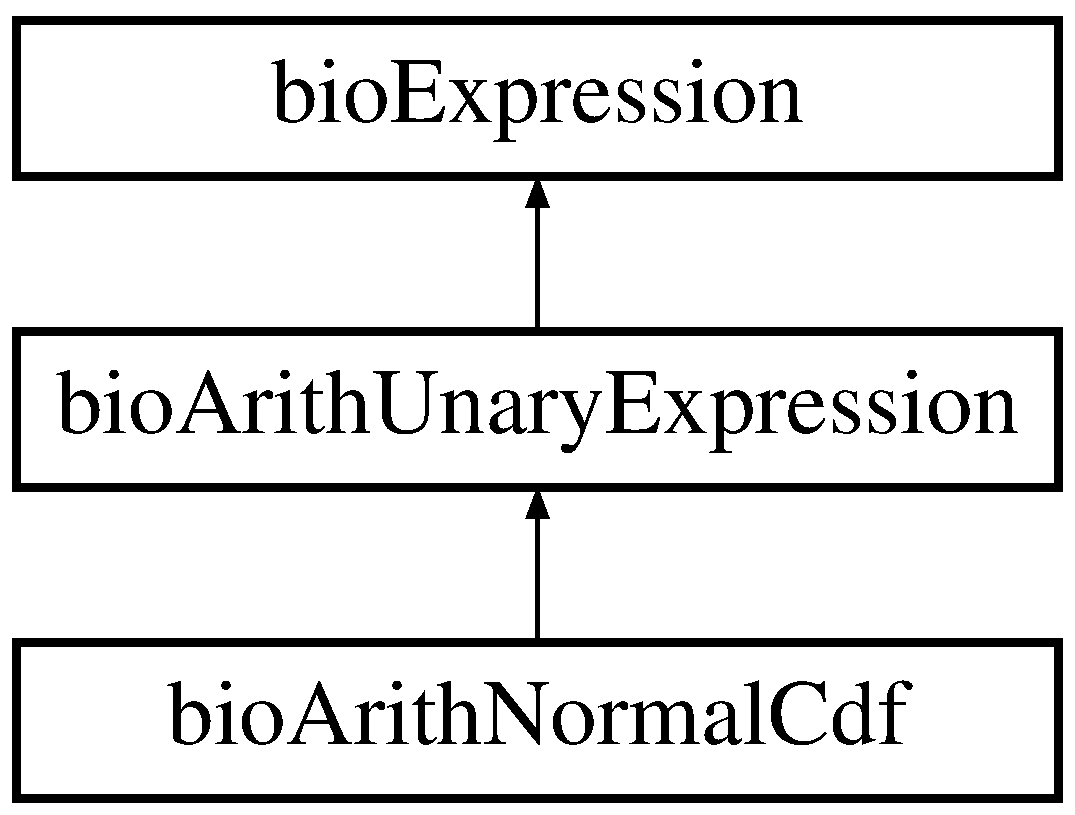
\includegraphics[height=3.000000cm]{classbio_arith_normal_cdf}
\end{center}
\end{figure}
\subsection*{Public Member Functions}
\begin{DoxyCompactItemize}
\item 
\mbox{\Hypertarget{classbio_arith_normal_cdf_a307bf9c59169fcd089379f7c5cd14226}\label{classbio_arith_normal_cdf_a307bf9c59169fcd089379f7c5cd14226}} 
{\bfseries bio\+Arith\+Normal\+Cdf} (\hyperlink{classbio_expression_repository}{bio\+Expression\+Repository} $\ast$rep, pat\+U\+Long par, pat\+U\+Long left, pat\+Error $\ast$\&err)
\item 
virtual pat\+String \hyperlink{classbio_arith_normal_cdf_a5c5a2ee63e4df2a8ccbc117bf819e48b}{get\+Operator\+Name} () const
\item 
virtual pat\+Real \hyperlink{classbio_arith_normal_cdf_abf66a564a8a244d62205d19484b63315}{get\+Value} (pat\+Boolean prepare\+Gradient, pat\+U\+Long current\+Lap, pat\+Error $\ast$\&err)
\item 
virtual \hyperlink{classbio_expression}{bio\+Expression} $\ast$ \hyperlink{classbio_arith_normal_cdf_adf643b1adb105be0728b921cd96d555f}{get\+Derivative} (pat\+U\+Long a\+Literal, pat\+Error $\ast$\&err) const
\item 
virtual \hyperlink{classbio_arith_normal_cdf}{bio\+Arith\+Normal\+Cdf} $\ast$ \hyperlink{classbio_arith_normal_cdf_ae88a5f7d19f32cc5daf01152931e9c62}{get\+Deep\+Copy} (\hyperlink{classbio_expression_repository}{bio\+Expression\+Repository} $\ast$rep, pat\+Error $\ast$\&err) const
\item 
virtual \hyperlink{classbio_arith_normal_cdf}{bio\+Arith\+Normal\+Cdf} $\ast$ \hyperlink{classbio_arith_normal_cdf_af05c8a2c466ed42e1f4b517b35b4be11}{get\+Shallow\+Copy} (\hyperlink{classbio_expression_repository}{bio\+Expression\+Repository} $\ast$rep, pat\+Error $\ast$\&err) const
\item 
virtual pat\+String \hyperlink{classbio_arith_normal_cdf_a2e5b58ae0d8b71d2129e7f44ff9c647e}{get\+Expression\+String} () const
\item 
virtual \hyperlink{classbio_function_and_derivatives}{bio\+Function\+And\+Derivatives} $\ast$ \hyperlink{classbio_arith_normal_cdf_ac482f8e85421635fd033018fd779ef88}{get\+Numerical\+Function\+And\+Gradient} (vector$<$ pat\+U\+Long $>$ literal\+Ids, pat\+Boolean compute\+Hessian, pat\+Boolean debug\+Derivatives, pat\+Error $\ast$\&err)
\end{DoxyCompactItemize}
\subsection*{Additional Inherited Members}


\subsection{Detailed Description}
Class implementing a node of the tree representing the C\+DF of the normal distribution 

\subsection{Member Function Documentation}
\mbox{\Hypertarget{classbio_arith_normal_cdf_ae88a5f7d19f32cc5daf01152931e9c62}\label{classbio_arith_normal_cdf_ae88a5f7d19f32cc5daf01152931e9c62}} 
\index{bio\+Arith\+Normal\+Cdf@{bio\+Arith\+Normal\+Cdf}!get\+Deep\+Copy@{get\+Deep\+Copy}}
\index{get\+Deep\+Copy@{get\+Deep\+Copy}!bio\+Arith\+Normal\+Cdf@{bio\+Arith\+Normal\+Cdf}}
\subsubsection{\texorpdfstring{get\+Deep\+Copy()}{getDeepCopy()}}
{\footnotesize\ttfamily \hyperlink{classbio_arith_normal_cdf}{bio\+Arith\+Normal\+Cdf} $\ast$ bio\+Arith\+Normal\+Cdf\+::get\+Deep\+Copy (\begin{DoxyParamCaption}\item[{\hyperlink{classbio_expression_repository}{bio\+Expression\+Repository} $\ast$}]{rep,  }\item[{pat\+Error $\ast$\&}]{err }\end{DoxyParamCaption}) const\hspace{0.3cm}{\ttfamily [virtual]}}

Create a deep copy of the expression and returns a pointer to it. It means that new instances of the children are created. 

Reimplemented from \hyperlink{classbio_expression_a4ee1b8add634078a02eaae26cd40dcc8}{bio\+Expression}.

\mbox{\Hypertarget{classbio_arith_normal_cdf_adf643b1adb105be0728b921cd96d555f}\label{classbio_arith_normal_cdf_adf643b1adb105be0728b921cd96d555f}} 
\index{bio\+Arith\+Normal\+Cdf@{bio\+Arith\+Normal\+Cdf}!get\+Derivative@{get\+Derivative}}
\index{get\+Derivative@{get\+Derivative}!bio\+Arith\+Normal\+Cdf@{bio\+Arith\+Normal\+Cdf}}
\subsubsection{\texorpdfstring{get\+Derivative()}{getDerivative()}}
{\footnotesize\ttfamily \hyperlink{classbio_expression}{bio\+Expression} $\ast$ bio\+Arith\+Normal\+Cdf\+::get\+Derivative (\begin{DoxyParamCaption}\item[{pat\+U\+Long}]{a\+Literal\+Id,  }\item[{pat\+Error $\ast$\&}]{err }\end{DoxyParamCaption}) const\hspace{0.3cm}{\ttfamily [virtual]}}

\begin{DoxyReturn}{Returns}
value of the derivative w.\+r.\+t literal 
\end{DoxyReturn}

\begin{DoxyParams}{Parameters}
{\em index} & of the literal involved in the derivative \\
\hline
{\em err} & ref. of the pointer to the error object. \\
\hline
\end{DoxyParams}


Reimplemented from \hyperlink{classbio_expression_a5915579d1193f25f216c1e273c97f2ce}{bio\+Expression}.

\mbox{\Hypertarget{classbio_arith_normal_cdf_a2e5b58ae0d8b71d2129e7f44ff9c647e}\label{classbio_arith_normal_cdf_a2e5b58ae0d8b71d2129e7f44ff9c647e}} 
\index{bio\+Arith\+Normal\+Cdf@{bio\+Arith\+Normal\+Cdf}!get\+Expression\+String@{get\+Expression\+String}}
\index{get\+Expression\+String@{get\+Expression\+String}!bio\+Arith\+Normal\+Cdf@{bio\+Arith\+Normal\+Cdf}}
\subsubsection{\texorpdfstring{get\+Expression\+String()}{getExpressionString()}}
{\footnotesize\ttfamily pat\+String bio\+Arith\+Normal\+Cdf\+::get\+Expression\+String (\begin{DoxyParamCaption}{ }\end{DoxyParamCaption}) const\hspace{0.3cm}{\ttfamily [virtual]}}

Compute a string that represents the expression. It is designed to replace the expression itself when used only for comparison purposes. Code\+: +\{expr1\}\{expr2\}\+: binary plus -\/\{expr1\}\{expr2\}\+: binary minus \{expr1\}\{expr2\}\+: multiplication /\{expr1\}\{expr2\}\+: division $^\wedge$\{expr1\}\{expr2\}\+: power \&\{expr1\}\{expr2\}\+: and $\vert$\{expr1\}\{expr2\}\+: or =\{expr1\}\{expr2\}\+: equal !=\{expr1\}\{expr2\}\+: not equal $<$\{expr1\}\{expr2\}\+: lesser than $<$=\{expr1\}\{expr2\}\+: lesser or equal to $>$\{expr1\}\{expr2\}\+: greater than $>$=\{expr1\}\{expr2\}\+: greater or equal to \$A\{expr\}\+: abs \$D\mbox{[}expr\mbox{]}\mbox{[}\{expr1\}...\{exprN\}\mbox{]}\+: dictionary (\hyperlink{classbio_arith_elem}{bio\+Arith\+Elem}) \$E\{expr\}\+: exp \$L\{expr\}\+: log \$M\{expr\}\+: Unary minus \$\+Piterator\+\_\+name\{expr\}\+: prod \$Q\{string1\}\{string2\}\+: sequence \$\+Siterator\+\_\+name\{expr\}\+: sum \$\+Ziterator\+\_\+name\mbox{[}\{expr1\}...\{exprN\}\mbox{]}\+: merged sum \{expr1\}\{expr2\}...\{exprN\}//\+: list of expressions number\+: constant \#id\+: literal \&id\+: random 

Reimplemented from \hyperlink{classbio_expression_a3e4b4dca58dbbc6f0e411b30eb3f60b4}{bio\+Expression}.

\mbox{\Hypertarget{classbio_arith_normal_cdf_ac482f8e85421635fd033018fd779ef88}\label{classbio_arith_normal_cdf_ac482f8e85421635fd033018fd779ef88}} 
\index{bio\+Arith\+Normal\+Cdf@{bio\+Arith\+Normal\+Cdf}!get\+Numerical\+Function\+And\+Gradient@{get\+Numerical\+Function\+And\+Gradient}}
\index{get\+Numerical\+Function\+And\+Gradient@{get\+Numerical\+Function\+And\+Gradient}!bio\+Arith\+Normal\+Cdf@{bio\+Arith\+Normal\+Cdf}}
\subsubsection{\texorpdfstring{get\+Numerical\+Function\+And\+Gradient()}{getNumericalFunctionAndGradient()}}
{\footnotesize\ttfamily \hyperlink{classbio_function_and_derivatives}{bio\+Function\+And\+Derivatives} $\ast$ bio\+Arith\+Normal\+Cdf\+::get\+Numerical\+Function\+And\+Gradient (\begin{DoxyParamCaption}\item[{vector$<$ pat\+U\+Long $>$}]{literal\+Ids,  }\item[{pat\+Boolean}]{compute\+Hessian,  }\item[{pat\+Boolean}]{debug\+Derivatives,  }\item[{pat\+Error $\ast$\&}]{err }\end{DoxyParamCaption})\hspace{0.3cm}{\ttfamily [virtual]}}

\begin{DoxyReturn}{Returns}
value and gradient of the expression 
\end{DoxyReturn}

\begin{DoxyParams}{Parameters}
{\em err} & ref. of the pointer to the error object. \\
\hline
\end{DoxyParams}


Reimplemented from \hyperlink{classbio_expression_a91c81ce80c9e972c913b10f5f3c1ed13}{bio\+Expression}.

\mbox{\Hypertarget{classbio_arith_normal_cdf_a5c5a2ee63e4df2a8ccbc117bf819e48b}\label{classbio_arith_normal_cdf_a5c5a2ee63e4df2a8ccbc117bf819e48b}} 
\index{bio\+Arith\+Normal\+Cdf@{bio\+Arith\+Normal\+Cdf}!get\+Operator\+Name@{get\+Operator\+Name}}
\index{get\+Operator\+Name@{get\+Operator\+Name}!bio\+Arith\+Normal\+Cdf@{bio\+Arith\+Normal\+Cdf}}
\subsubsection{\texorpdfstring{get\+Operator\+Name()}{getOperatorName()}}
{\footnotesize\ttfamily pat\+String bio\+Arith\+Normal\+Cdf\+::get\+Operator\+Name (\begin{DoxyParamCaption}{ }\end{DoxyParamCaption}) const\hspace{0.3cm}{\ttfamily [virtual]}}

\begin{DoxyReturn}{Returns}
name of the operator 
\end{DoxyReturn}


Reimplemented from \hyperlink{classbio_expression_a2353a4afb3a2b0af7c63aba086a72bde}{bio\+Expression}.

\mbox{\Hypertarget{classbio_arith_normal_cdf_af05c8a2c466ed42e1f4b517b35b4be11}\label{classbio_arith_normal_cdf_af05c8a2c466ed42e1f4b517b35b4be11}} 
\index{bio\+Arith\+Normal\+Cdf@{bio\+Arith\+Normal\+Cdf}!get\+Shallow\+Copy@{get\+Shallow\+Copy}}
\index{get\+Shallow\+Copy@{get\+Shallow\+Copy}!bio\+Arith\+Normal\+Cdf@{bio\+Arith\+Normal\+Cdf}}
\subsubsection{\texorpdfstring{get\+Shallow\+Copy()}{getShallowCopy()}}
{\footnotesize\ttfamily \hyperlink{classbio_arith_normal_cdf}{bio\+Arith\+Normal\+Cdf} $\ast$ bio\+Arith\+Normal\+Cdf\+::get\+Shallow\+Copy (\begin{DoxyParamCaption}\item[{\hyperlink{classbio_expression_repository}{bio\+Expression\+Repository} $\ast$}]{rep,  }\item[{pat\+Error $\ast$\&}]{err }\end{DoxyParamCaption}) const\hspace{0.3cm}{\ttfamily [virtual]}}

Create a shallow copy of the expression and returns a pointer to it. It means that no new instance of the children are created. It is typically called by the repository 

Reimplemented from \hyperlink{classbio_expression_a442534762693b92baaf33928979a1bf8}{bio\+Expression}.

\mbox{\Hypertarget{classbio_arith_normal_cdf_abf66a564a8a244d62205d19484b63315}\label{classbio_arith_normal_cdf_abf66a564a8a244d62205d19484b63315}} 
\index{bio\+Arith\+Normal\+Cdf@{bio\+Arith\+Normal\+Cdf}!get\+Value@{get\+Value}}
\index{get\+Value@{get\+Value}!bio\+Arith\+Normal\+Cdf@{bio\+Arith\+Normal\+Cdf}}
\subsubsection{\texorpdfstring{get\+Value()}{getValue()}}
{\footnotesize\ttfamily pat\+Real bio\+Arith\+Normal\+Cdf\+::get\+Value (\begin{DoxyParamCaption}\item[{pat\+Boolean}]{prepare\+Gradient,  }\item[{pat\+U\+Long}]{current\+Lap,  }\item[{pat\+Error $\ast$\&}]{err }\end{DoxyParamCaption})\hspace{0.3cm}{\ttfamily [virtual]}}

\begin{DoxyReturn}{Returns}
value of the expression 
\end{DoxyReturn}

\begin{DoxyParams}{Parameters}
{\em err} & ref. of the pointer to the error object. \\
\hline
\end{DoxyParams}


Reimplemented from \hyperlink{classbio_expression_af58662a5d4d456f15bc4f2c9bd4f8a5b}{bio\+Expression}.



The documentation for this class was generated from the following files\+:\begin{DoxyCompactItemize}
\item 
bio\+Arith\+Normal\+Cdf.\+h\item 
bio\+Arith\+Normal\+Cdf.\+cc\end{DoxyCompactItemize}

\hypertarget{classbio_arith_normal_pdf}{}\section{bio\+Arith\+Normal\+Pdf Class Reference}
\label{classbio_arith_normal_pdf}\index{bio\+Arith\+Normal\+Pdf@{bio\+Arith\+Normal\+Pdf}}


{\ttfamily \#include $<$bio\+Arith\+Normal\+Pdf.\+h$>$}

Inheritance diagram for bio\+Arith\+Normal\+Pdf\+:\begin{figure}[H]
\begin{center}
\leavevmode
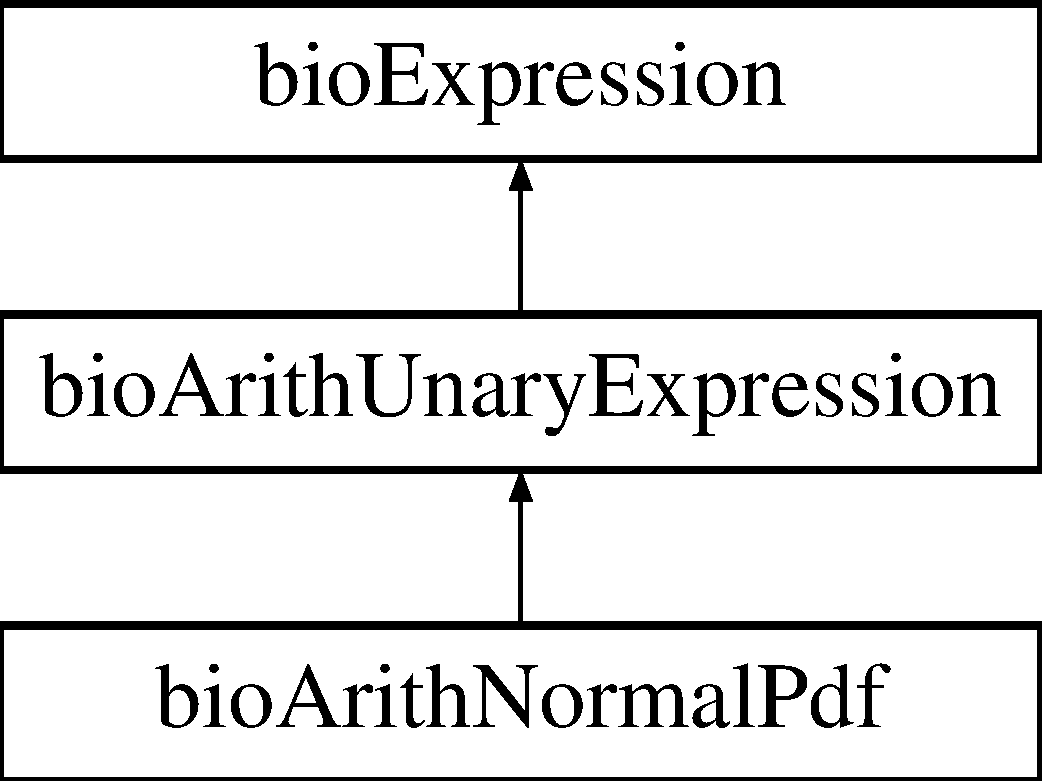
\includegraphics[height=3.000000cm]{classbio_arith_normal_pdf}
\end{center}
\end{figure}
\subsection*{Public Member Functions}
\begin{DoxyCompactItemize}
\item 
\mbox{\Hypertarget{classbio_arith_normal_pdf_a65b70d94c42bc2e70ac52b7dba179db1}\label{classbio_arith_normal_pdf_a65b70d94c42bc2e70ac52b7dba179db1}} 
{\bfseries bio\+Arith\+Normal\+Pdf} (\hyperlink{classbio_expression_repository}{bio\+Expression\+Repository} $\ast$rep, pat\+U\+Long par, pat\+U\+Long left, pat\+Error $\ast$\&err)
\item 
virtual pat\+String \hyperlink{classbio_arith_normal_pdf_ae2ad20d8db8f935fa7de1f4a0fd3288e}{get\+Operator\+Name} () const
\item 
virtual pat\+Real \hyperlink{classbio_arith_normal_pdf_a6b9af77b48e6a3eb8441df836be67d40}{get\+Value} (pat\+Boolean prepare\+Gradient, pat\+U\+Long current\+Lap, pat\+Error $\ast$\&err)
\item 
virtual \hyperlink{classbio_expression}{bio\+Expression} $\ast$ \hyperlink{classbio_arith_normal_pdf_a25ab081a2c88449126a328a5eb635818}{get\+Derivative} (pat\+U\+Long a\+Literal\+Id, pat\+Error $\ast$\&err) const
\item 
virtual \hyperlink{classbio_arith_normal_pdf}{bio\+Arith\+Normal\+Pdf} $\ast$ \hyperlink{classbio_arith_normal_pdf_af001f9bda79d1518e2c9913c02f98a37}{get\+Deep\+Copy} (\hyperlink{classbio_expression_repository}{bio\+Expression\+Repository} $\ast$rep, pat\+Error $\ast$\&err) const
\item 
virtual \hyperlink{classbio_arith_normal_pdf}{bio\+Arith\+Normal\+Pdf} $\ast$ \hyperlink{classbio_arith_normal_pdf_aeec0c66c4ba5c8ae0ee9d35be0bf1eb9}{get\+Shallow\+Copy} (\hyperlink{classbio_expression_repository}{bio\+Expression\+Repository} $\ast$rep, pat\+Error $\ast$\&err) const
\item 
virtual pat\+String \hyperlink{classbio_arith_normal_pdf_af63b696ee818be0597345caf08d0b3d1}{get\+Expression\+String} () const
\item 
virtual \hyperlink{classbio_function_and_derivatives}{bio\+Function\+And\+Derivatives} $\ast$ \hyperlink{classbio_arith_normal_pdf_ab55fce91dd0740f61c7026426602e996}{get\+Numerical\+Function\+And\+Gradient} (vector$<$ pat\+U\+Long $>$ literal\+Ids, pat\+Boolean compute\+Hessian, pat\+Boolean debug\+Derivatives, pat\+Error $\ast$\&err)
\end{DoxyCompactItemize}
\subsection*{Additional Inherited Members}


\subsection{Detailed Description}
We have a dictionary of utilities, mapping values to utilities. 

\subsection{Member Function Documentation}
\mbox{\Hypertarget{classbio_arith_normal_pdf_af001f9bda79d1518e2c9913c02f98a37}\label{classbio_arith_normal_pdf_af001f9bda79d1518e2c9913c02f98a37}} 
\index{bio\+Arith\+Normal\+Pdf@{bio\+Arith\+Normal\+Pdf}!get\+Deep\+Copy@{get\+Deep\+Copy}}
\index{get\+Deep\+Copy@{get\+Deep\+Copy}!bio\+Arith\+Normal\+Pdf@{bio\+Arith\+Normal\+Pdf}}
\subsubsection{\texorpdfstring{get\+Deep\+Copy()}{getDeepCopy()}}
{\footnotesize\ttfamily \hyperlink{classbio_arith_normal_pdf}{bio\+Arith\+Normal\+Pdf} $\ast$ bio\+Arith\+Normal\+Pdf\+::get\+Deep\+Copy (\begin{DoxyParamCaption}\item[{\hyperlink{classbio_expression_repository}{bio\+Expression\+Repository} $\ast$}]{rep,  }\item[{pat\+Error $\ast$\&}]{err }\end{DoxyParamCaption}) const\hspace{0.3cm}{\ttfamily [virtual]}}

Create a deep copy of the expression and returns a pointer to it. It means that new instances of the children are created. 

Reimplemented from \hyperlink{classbio_expression_a4ee1b8add634078a02eaae26cd40dcc8}{bio\+Expression}.

\mbox{\Hypertarget{classbio_arith_normal_pdf_a25ab081a2c88449126a328a5eb635818}\label{classbio_arith_normal_pdf_a25ab081a2c88449126a328a5eb635818}} 
\index{bio\+Arith\+Normal\+Pdf@{bio\+Arith\+Normal\+Pdf}!get\+Derivative@{get\+Derivative}}
\index{get\+Derivative@{get\+Derivative}!bio\+Arith\+Normal\+Pdf@{bio\+Arith\+Normal\+Pdf}}
\subsubsection{\texorpdfstring{get\+Derivative()}{getDerivative()}}
{\footnotesize\ttfamily \hyperlink{classbio_expression}{bio\+Expression} $\ast$ bio\+Arith\+Normal\+Pdf\+::get\+Derivative (\begin{DoxyParamCaption}\item[{pat\+U\+Long}]{a\+Literal\+Id,  }\item[{pat\+Error $\ast$\&}]{err }\end{DoxyParamCaption}) const\hspace{0.3cm}{\ttfamily [virtual]}}

\begin{DoxyReturn}{Returns}
value of the derivative w.\+r.\+t literal 
\end{DoxyReturn}

\begin{DoxyParams}{Parameters}
{\em index} & of the literal involved in the derivative \\
\hline
{\em err} & ref. of the pointer to the error object. \\
\hline
\end{DoxyParams}


Reimplemented from \hyperlink{classbio_expression_a5915579d1193f25f216c1e273c97f2ce}{bio\+Expression}.

\mbox{\Hypertarget{classbio_arith_normal_pdf_af63b696ee818be0597345caf08d0b3d1}\label{classbio_arith_normal_pdf_af63b696ee818be0597345caf08d0b3d1}} 
\index{bio\+Arith\+Normal\+Pdf@{bio\+Arith\+Normal\+Pdf}!get\+Expression\+String@{get\+Expression\+String}}
\index{get\+Expression\+String@{get\+Expression\+String}!bio\+Arith\+Normal\+Pdf@{bio\+Arith\+Normal\+Pdf}}
\subsubsection{\texorpdfstring{get\+Expression\+String()}{getExpressionString()}}
{\footnotesize\ttfamily pat\+String bio\+Arith\+Normal\+Pdf\+::get\+Expression\+String (\begin{DoxyParamCaption}{ }\end{DoxyParamCaption}) const\hspace{0.3cm}{\ttfamily [virtual]}}

Compute a string that represents the expression. It is designed to replace the expression itself when used only for comparison purposes. Code\+: +\{expr1\}\{expr2\}\+: binary plus -\/\{expr1\}\{expr2\}\+: binary minus \{expr1\}\{expr2\}\+: multiplication /\{expr1\}\{expr2\}\+: division $^\wedge$\{expr1\}\{expr2\}\+: power \&\{expr1\}\{expr2\}\+: and $\vert$\{expr1\}\{expr2\}\+: or =\{expr1\}\{expr2\}\+: equal !=\{expr1\}\{expr2\}\+: not equal $<$\{expr1\}\{expr2\}\+: lesser than $<$=\{expr1\}\{expr2\}\+: lesser or equal to $>$\{expr1\}\{expr2\}\+: greater than $>$=\{expr1\}\{expr2\}\+: greater or equal to \$A\{expr\}\+: abs \$D\mbox{[}expr\mbox{]}\mbox{[}\{expr1\}...\{exprN\}\mbox{]}\+: dictionary (\hyperlink{classbio_arith_elem}{bio\+Arith\+Elem}) \$E\{expr\}\+: exp \$L\{expr\}\+: log \$M\{expr\}\+: Unary minus \$\+Piterator\+\_\+name\{expr\}\+: prod \$Q\{string1\}\{string2\}\+: sequence \$\+Siterator\+\_\+name\{expr\}\+: sum \$\+Ziterator\+\_\+name\mbox{[}\{expr1\}...\{exprN\}\mbox{]}\+: merged sum \{expr1\}\{expr2\}...\{exprN\}//\+: list of expressions number\+: constant \#id\+: literal \&id\+: random 

Reimplemented from \hyperlink{classbio_expression_a3e4b4dca58dbbc6f0e411b30eb3f60b4}{bio\+Expression}.

\mbox{\Hypertarget{classbio_arith_normal_pdf_ab55fce91dd0740f61c7026426602e996}\label{classbio_arith_normal_pdf_ab55fce91dd0740f61c7026426602e996}} 
\index{bio\+Arith\+Normal\+Pdf@{bio\+Arith\+Normal\+Pdf}!get\+Numerical\+Function\+And\+Gradient@{get\+Numerical\+Function\+And\+Gradient}}
\index{get\+Numerical\+Function\+And\+Gradient@{get\+Numerical\+Function\+And\+Gradient}!bio\+Arith\+Normal\+Pdf@{bio\+Arith\+Normal\+Pdf}}
\subsubsection{\texorpdfstring{get\+Numerical\+Function\+And\+Gradient()}{getNumericalFunctionAndGradient()}}
{\footnotesize\ttfamily \hyperlink{classbio_function_and_derivatives}{bio\+Function\+And\+Derivatives} $\ast$ bio\+Arith\+Normal\+Pdf\+::get\+Numerical\+Function\+And\+Gradient (\begin{DoxyParamCaption}\item[{vector$<$ pat\+U\+Long $>$}]{literal\+Ids,  }\item[{pat\+Boolean}]{compute\+Hessian,  }\item[{pat\+Boolean}]{debug\+Derivatives,  }\item[{pat\+Error $\ast$\&}]{err }\end{DoxyParamCaption})\hspace{0.3cm}{\ttfamily [virtual]}}

\begin{DoxyReturn}{Returns}
value and gradient of the expression 
\end{DoxyReturn}

\begin{DoxyParams}{Parameters}
{\em err} & ref. of the pointer to the error object. \\
\hline
\end{DoxyParams}


Reimplemented from \hyperlink{classbio_expression_a91c81ce80c9e972c913b10f5f3c1ed13}{bio\+Expression}.

\mbox{\Hypertarget{classbio_arith_normal_pdf_ae2ad20d8db8f935fa7de1f4a0fd3288e}\label{classbio_arith_normal_pdf_ae2ad20d8db8f935fa7de1f4a0fd3288e}} 
\index{bio\+Arith\+Normal\+Pdf@{bio\+Arith\+Normal\+Pdf}!get\+Operator\+Name@{get\+Operator\+Name}}
\index{get\+Operator\+Name@{get\+Operator\+Name}!bio\+Arith\+Normal\+Pdf@{bio\+Arith\+Normal\+Pdf}}
\subsubsection{\texorpdfstring{get\+Operator\+Name()}{getOperatorName()}}
{\footnotesize\ttfamily pat\+String bio\+Arith\+Normal\+Pdf\+::get\+Operator\+Name (\begin{DoxyParamCaption}{ }\end{DoxyParamCaption}) const\hspace{0.3cm}{\ttfamily [virtual]}}

\begin{DoxyReturn}{Returns}
name of the operator 
\end{DoxyReturn}


Reimplemented from \hyperlink{classbio_expression_a2353a4afb3a2b0af7c63aba086a72bde}{bio\+Expression}.

\mbox{\Hypertarget{classbio_arith_normal_pdf_aeec0c66c4ba5c8ae0ee9d35be0bf1eb9}\label{classbio_arith_normal_pdf_aeec0c66c4ba5c8ae0ee9d35be0bf1eb9}} 
\index{bio\+Arith\+Normal\+Pdf@{bio\+Arith\+Normal\+Pdf}!get\+Shallow\+Copy@{get\+Shallow\+Copy}}
\index{get\+Shallow\+Copy@{get\+Shallow\+Copy}!bio\+Arith\+Normal\+Pdf@{bio\+Arith\+Normal\+Pdf}}
\subsubsection{\texorpdfstring{get\+Shallow\+Copy()}{getShallowCopy()}}
{\footnotesize\ttfamily \hyperlink{classbio_arith_normal_pdf}{bio\+Arith\+Normal\+Pdf} $\ast$ bio\+Arith\+Normal\+Pdf\+::get\+Shallow\+Copy (\begin{DoxyParamCaption}\item[{\hyperlink{classbio_expression_repository}{bio\+Expression\+Repository} $\ast$}]{rep,  }\item[{pat\+Error $\ast$\&}]{err }\end{DoxyParamCaption}) const\hspace{0.3cm}{\ttfamily [virtual]}}

Create a shallow copy of the expression and returns a pointer to it. It means that no new instance of the children are created. It is typically called by the repository 

Reimplemented from \hyperlink{classbio_expression_a442534762693b92baaf33928979a1bf8}{bio\+Expression}.

\mbox{\Hypertarget{classbio_arith_normal_pdf_a6b9af77b48e6a3eb8441df836be67d40}\label{classbio_arith_normal_pdf_a6b9af77b48e6a3eb8441df836be67d40}} 
\index{bio\+Arith\+Normal\+Pdf@{bio\+Arith\+Normal\+Pdf}!get\+Value@{get\+Value}}
\index{get\+Value@{get\+Value}!bio\+Arith\+Normal\+Pdf@{bio\+Arith\+Normal\+Pdf}}
\subsubsection{\texorpdfstring{get\+Value()}{getValue()}}
{\footnotesize\ttfamily pat\+Real bio\+Arith\+Normal\+Pdf\+::get\+Value (\begin{DoxyParamCaption}\item[{pat\+Boolean}]{prepare\+Gradient,  }\item[{pat\+U\+Long}]{current\+Lap,  }\item[{pat\+Error $\ast$\&}]{err }\end{DoxyParamCaption})\hspace{0.3cm}{\ttfamily [virtual]}}

\begin{DoxyReturn}{Returns}
value of the expression 
\end{DoxyReturn}

\begin{DoxyParams}{Parameters}
{\em err} & ref. of the pointer to the error object. \\
\hline
\end{DoxyParams}


Reimplemented from \hyperlink{classbio_expression_af58662a5d4d456f15bc4f2c9bd4f8a5b}{bio\+Expression}.



The documentation for this class was generated from the following files\+:\begin{DoxyCompactItemize}
\item 
bio\+Arith\+Normal\+Pdf.\+h\item 
bio\+Arith\+Normal\+Pdf.\+cc\end{DoxyCompactItemize}

\hypertarget{classbio_arith_not_equal}{}\section{bio\+Arith\+Not\+Equal Class Reference}
\label{classbio_arith_not_equal}\index{bio\+Arith\+Not\+Equal@{bio\+Arith\+Not\+Equal}}


{\ttfamily \#include $<$bio\+Arith\+Not\+Equal.\+h$>$}

Inheritance diagram for bio\+Arith\+Not\+Equal\+:\begin{figure}[H]
\begin{center}
\leavevmode
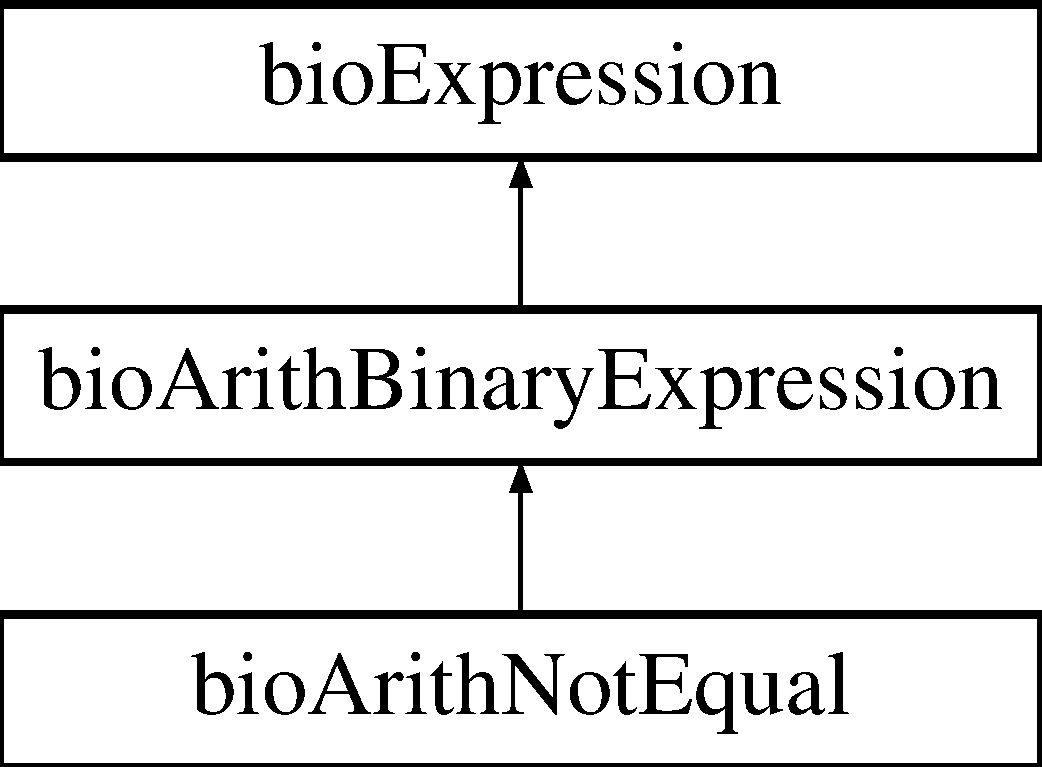
\includegraphics[height=3.000000cm]{classbio_arith_not_equal}
\end{center}
\end{figure}
\subsection*{Public Member Functions}
\begin{DoxyCompactItemize}
\item 
\mbox{\Hypertarget{classbio_arith_not_equal_ae92be935b4ddc30c035a0c6ddcf5e891}\label{classbio_arith_not_equal_ae92be935b4ddc30c035a0c6ddcf5e891}} 
{\bfseries bio\+Arith\+Not\+Equal} (\hyperlink{classbio_expression_repository}{bio\+Expression\+Repository} $\ast$rep, pat\+U\+Long par, pat\+U\+Long left, pat\+U\+Long right, pat\+Error $\ast$\&err)
\item 
virtual pat\+String \hyperlink{classbio_arith_not_equal_a70bfdbd3473869466dc02e026620996c}{get\+Operator\+Name} () const
\item 
virtual pat\+Real \hyperlink{classbio_arith_not_equal_aa081815819ab133fa2fbfc87ecef0e66}{get\+Value} (pat\+Boolean prepare\+Gradient, pat\+U\+Long current\+Lap, pat\+Error $\ast$\&err)
\item 
virtual \hyperlink{classbio_expression}{bio\+Expression} $\ast$ \hyperlink{classbio_arith_not_equal_ad06316415449cf1af6657a9932f819e2}{get\+Derivative} (pat\+U\+Long a\+Literal, pat\+Error $\ast$\&err) const
\item 
virtual \hyperlink{classbio_arith_not_equal}{bio\+Arith\+Not\+Equal} $\ast$ \hyperlink{classbio_arith_not_equal_a6b6319667f2a08c63854edfbd2cae799}{get\+Deep\+Copy} (\hyperlink{classbio_expression_repository}{bio\+Expression\+Repository} $\ast$rep, pat\+Error $\ast$\&err) const
\item 
virtual \hyperlink{classbio_arith_not_equal}{bio\+Arith\+Not\+Equal} $\ast$ \hyperlink{classbio_arith_not_equal_a22bcfcb7855cf992f9dc39d0911cebb5}{get\+Shallow\+Copy} (\hyperlink{classbio_expression_repository}{bio\+Expression\+Repository} $\ast$rep, pat\+Error $\ast$\&err) const
\item 
virtual pat\+String \hyperlink{classbio_arith_not_equal_a8fe4fd578218783f3a18665eae9f750c}{get\+Expression\+String} () const
\item 
virtual \hyperlink{classbio_function_and_derivatives}{bio\+Function\+And\+Derivatives} $\ast$ \hyperlink{classbio_arith_not_equal_ad9f06b2145f70fc6ebebc5bca51b5aa8}{get\+Numerical\+Function\+And\+Gradient} (vector$<$ pat\+U\+Long $>$ literal\+Ids, pat\+Boolean compute\+Hessian, pat\+Boolean debug\+Derivatives, pat\+Error $\ast$\&err)
\end{DoxyCompactItemize}
\subsection*{Additional Inherited Members}


\subsection{Detailed Description}
Class implementing a node of the tree representing a comparison (!=) operation 

\subsection{Member Function Documentation}
\mbox{\Hypertarget{classbio_arith_not_equal_a6b6319667f2a08c63854edfbd2cae799}\label{classbio_arith_not_equal_a6b6319667f2a08c63854edfbd2cae799}} 
\index{bio\+Arith\+Not\+Equal@{bio\+Arith\+Not\+Equal}!get\+Deep\+Copy@{get\+Deep\+Copy}}
\index{get\+Deep\+Copy@{get\+Deep\+Copy}!bio\+Arith\+Not\+Equal@{bio\+Arith\+Not\+Equal}}
\subsubsection{\texorpdfstring{get\+Deep\+Copy()}{getDeepCopy()}}
{\footnotesize\ttfamily \hyperlink{classbio_arith_not_equal}{bio\+Arith\+Not\+Equal} $\ast$ bio\+Arith\+Not\+Equal\+::get\+Deep\+Copy (\begin{DoxyParamCaption}\item[{\hyperlink{classbio_expression_repository}{bio\+Expression\+Repository} $\ast$}]{rep,  }\item[{pat\+Error $\ast$\&}]{err }\end{DoxyParamCaption}) const\hspace{0.3cm}{\ttfamily [virtual]}}

Create a deep copy of the expression and returns a pointer to it. It means that new instances of the children are created. 

Reimplemented from \hyperlink{classbio_expression_a4ee1b8add634078a02eaae26cd40dcc8}{bio\+Expression}.

\mbox{\Hypertarget{classbio_arith_not_equal_ad06316415449cf1af6657a9932f819e2}\label{classbio_arith_not_equal_ad06316415449cf1af6657a9932f819e2}} 
\index{bio\+Arith\+Not\+Equal@{bio\+Arith\+Not\+Equal}!get\+Derivative@{get\+Derivative}}
\index{get\+Derivative@{get\+Derivative}!bio\+Arith\+Not\+Equal@{bio\+Arith\+Not\+Equal}}
\subsubsection{\texorpdfstring{get\+Derivative()}{getDerivative()}}
{\footnotesize\ttfamily \hyperlink{classbio_expression}{bio\+Expression} $\ast$ bio\+Arith\+Not\+Equal\+::get\+Derivative (\begin{DoxyParamCaption}\item[{pat\+U\+Long}]{a\+Literal\+Id,  }\item[{pat\+Error $\ast$\&}]{err }\end{DoxyParamCaption}) const\hspace{0.3cm}{\ttfamily [virtual]}}

\begin{DoxyReturn}{Returns}
value of the derivative w.\+r.\+t literal 
\end{DoxyReturn}

\begin{DoxyParams}{Parameters}
{\em index} & of the literal involved in the derivative \\
\hline
{\em err} & ref. of the pointer to the error object. \\
\hline
\end{DoxyParams}


Reimplemented from \hyperlink{classbio_expression_a5915579d1193f25f216c1e273c97f2ce}{bio\+Expression}.

\mbox{\Hypertarget{classbio_arith_not_equal_a8fe4fd578218783f3a18665eae9f750c}\label{classbio_arith_not_equal_a8fe4fd578218783f3a18665eae9f750c}} 
\index{bio\+Arith\+Not\+Equal@{bio\+Arith\+Not\+Equal}!get\+Expression\+String@{get\+Expression\+String}}
\index{get\+Expression\+String@{get\+Expression\+String}!bio\+Arith\+Not\+Equal@{bio\+Arith\+Not\+Equal}}
\subsubsection{\texorpdfstring{get\+Expression\+String()}{getExpressionString()}}
{\footnotesize\ttfamily pat\+String bio\+Arith\+Not\+Equal\+::get\+Expression\+String (\begin{DoxyParamCaption}{ }\end{DoxyParamCaption}) const\hspace{0.3cm}{\ttfamily [virtual]}}

Compute a string that represents the expression. It is designed to replace the expression itself when used only for comparison purposes. Code\+: +\{expr1\}\{expr2\}\+: binary plus -\/\{expr1\}\{expr2\}\+: binary minus \{expr1\}\{expr2\}\+: multiplication /\{expr1\}\{expr2\}\+: division $^\wedge$\{expr1\}\{expr2\}\+: power \&\{expr1\}\{expr2\}\+: and $\vert$\{expr1\}\{expr2\}\+: or =\{expr1\}\{expr2\}\+: equal !=\{expr1\}\{expr2\}\+: not equal $<$\{expr1\}\{expr2\}\+: lesser than $<$=\{expr1\}\{expr2\}\+: lesser or equal to $>$\{expr1\}\{expr2\}\+: greater than $>$=\{expr1\}\{expr2\}\+: greater or equal to \$A\{expr\}\+: abs \$D\mbox{[}expr\mbox{]}\mbox{[}\{expr1\}...\{exprN\}\mbox{]}\+: dictionary (\hyperlink{classbio_arith_elem}{bio\+Arith\+Elem}) \$E\{expr\}\+: exp \$L\{expr\}\+: log \$M\{expr\}\+: Unary minus \$\+Piterator\+\_\+name\{expr\}\+: prod \$Q\{string1\}\{string2\}\+: sequence \$\+Siterator\+\_\+name\{expr\}\+: sum \$\+Ziterator\+\_\+name\mbox{[}\{expr1\}...\{exprN\}\mbox{]}\+: merged sum \{expr1\}\{expr2\}...\{exprN\}//\+: list of expressions number\+: constant \#id\+: literal \&id\+: random 

Reimplemented from \hyperlink{classbio_expression_a3e4b4dca58dbbc6f0e411b30eb3f60b4}{bio\+Expression}.

\mbox{\Hypertarget{classbio_arith_not_equal_ad9f06b2145f70fc6ebebc5bca51b5aa8}\label{classbio_arith_not_equal_ad9f06b2145f70fc6ebebc5bca51b5aa8}} 
\index{bio\+Arith\+Not\+Equal@{bio\+Arith\+Not\+Equal}!get\+Numerical\+Function\+And\+Gradient@{get\+Numerical\+Function\+And\+Gradient}}
\index{get\+Numerical\+Function\+And\+Gradient@{get\+Numerical\+Function\+And\+Gradient}!bio\+Arith\+Not\+Equal@{bio\+Arith\+Not\+Equal}}
\subsubsection{\texorpdfstring{get\+Numerical\+Function\+And\+Gradient()}{getNumericalFunctionAndGradient()}}
{\footnotesize\ttfamily \hyperlink{classbio_function_and_derivatives}{bio\+Function\+And\+Derivatives} $\ast$ bio\+Arith\+Not\+Equal\+::get\+Numerical\+Function\+And\+Gradient (\begin{DoxyParamCaption}\item[{vector$<$ pat\+U\+Long $>$}]{literal\+Ids,  }\item[{pat\+Boolean}]{compute\+Hessian,  }\item[{pat\+Boolean}]{debug\+Derivatives,  }\item[{pat\+Error $\ast$\&}]{err }\end{DoxyParamCaption})\hspace{0.3cm}{\ttfamily [virtual]}}

\begin{DoxyReturn}{Returns}
value and gradient of the expression 
\end{DoxyReturn}

\begin{DoxyParams}{Parameters}
{\em err} & ref. of the pointer to the error object. \\
\hline
\end{DoxyParams}


Reimplemented from \hyperlink{classbio_expression_a91c81ce80c9e972c913b10f5f3c1ed13}{bio\+Expression}.

\mbox{\Hypertarget{classbio_arith_not_equal_a70bfdbd3473869466dc02e026620996c}\label{classbio_arith_not_equal_a70bfdbd3473869466dc02e026620996c}} 
\index{bio\+Arith\+Not\+Equal@{bio\+Arith\+Not\+Equal}!get\+Operator\+Name@{get\+Operator\+Name}}
\index{get\+Operator\+Name@{get\+Operator\+Name}!bio\+Arith\+Not\+Equal@{bio\+Arith\+Not\+Equal}}
\subsubsection{\texorpdfstring{get\+Operator\+Name()}{getOperatorName()}}
{\footnotesize\ttfamily pat\+String bio\+Arith\+Not\+Equal\+::get\+Operator\+Name (\begin{DoxyParamCaption}{ }\end{DoxyParamCaption}) const\hspace{0.3cm}{\ttfamily [virtual]}}

\begin{DoxyReturn}{Returns}
name of the operator 
\end{DoxyReturn}


Reimplemented from \hyperlink{classbio_expression_a2353a4afb3a2b0af7c63aba086a72bde}{bio\+Expression}.

\mbox{\Hypertarget{classbio_arith_not_equal_a22bcfcb7855cf992f9dc39d0911cebb5}\label{classbio_arith_not_equal_a22bcfcb7855cf992f9dc39d0911cebb5}} 
\index{bio\+Arith\+Not\+Equal@{bio\+Arith\+Not\+Equal}!get\+Shallow\+Copy@{get\+Shallow\+Copy}}
\index{get\+Shallow\+Copy@{get\+Shallow\+Copy}!bio\+Arith\+Not\+Equal@{bio\+Arith\+Not\+Equal}}
\subsubsection{\texorpdfstring{get\+Shallow\+Copy()}{getShallowCopy()}}
{\footnotesize\ttfamily \hyperlink{classbio_arith_not_equal}{bio\+Arith\+Not\+Equal} $\ast$ bio\+Arith\+Not\+Equal\+::get\+Shallow\+Copy (\begin{DoxyParamCaption}\item[{\hyperlink{classbio_expression_repository}{bio\+Expression\+Repository} $\ast$}]{rep,  }\item[{pat\+Error $\ast$\&}]{err }\end{DoxyParamCaption}) const\hspace{0.3cm}{\ttfamily [virtual]}}

Create a shallow copy of the expression and returns a pointer to it. It means that no new instance of the children are created. It is typically called by the repository 

Reimplemented from \hyperlink{classbio_expression_a442534762693b92baaf33928979a1bf8}{bio\+Expression}.

\mbox{\Hypertarget{classbio_arith_not_equal_aa081815819ab133fa2fbfc87ecef0e66}\label{classbio_arith_not_equal_aa081815819ab133fa2fbfc87ecef0e66}} 
\index{bio\+Arith\+Not\+Equal@{bio\+Arith\+Not\+Equal}!get\+Value@{get\+Value}}
\index{get\+Value@{get\+Value}!bio\+Arith\+Not\+Equal@{bio\+Arith\+Not\+Equal}}
\subsubsection{\texorpdfstring{get\+Value()}{getValue()}}
{\footnotesize\ttfamily pat\+Real bio\+Arith\+Not\+Equal\+::get\+Value (\begin{DoxyParamCaption}\item[{pat\+Boolean}]{prepare\+Gradient,  }\item[{pat\+U\+Long}]{current\+Lap,  }\item[{pat\+Error $\ast$\&}]{err }\end{DoxyParamCaption})\hspace{0.3cm}{\ttfamily [virtual]}}

\begin{DoxyReturn}{Returns}
value of the expression 
\end{DoxyReturn}

\begin{DoxyParams}{Parameters}
{\em err} & ref. of the pointer to the error object. \\
\hline
\end{DoxyParams}


Reimplemented from \hyperlink{classbio_expression_af58662a5d4d456f15bc4f2c9bd4f8a5b}{bio\+Expression}.



The documentation for this class was generated from the following files\+:\begin{DoxyCompactItemize}
\item 
bio\+Arith\+Not\+Equal.\+h\item 
bio\+Arith\+Not\+Equal.\+cc\end{DoxyCompactItemize}

\hypertarget{classbio_arith_or}{}\section{bio\+Arith\+Or Class Reference}
\label{classbio_arith_or}\index{bio\+Arith\+Or@{bio\+Arith\+Or}}


{\ttfamily \#include $<$bio\+Arith\+Or.\+h$>$}

Inheritance diagram for bio\+Arith\+Or\+:\begin{figure}[H]
\begin{center}
\leavevmode
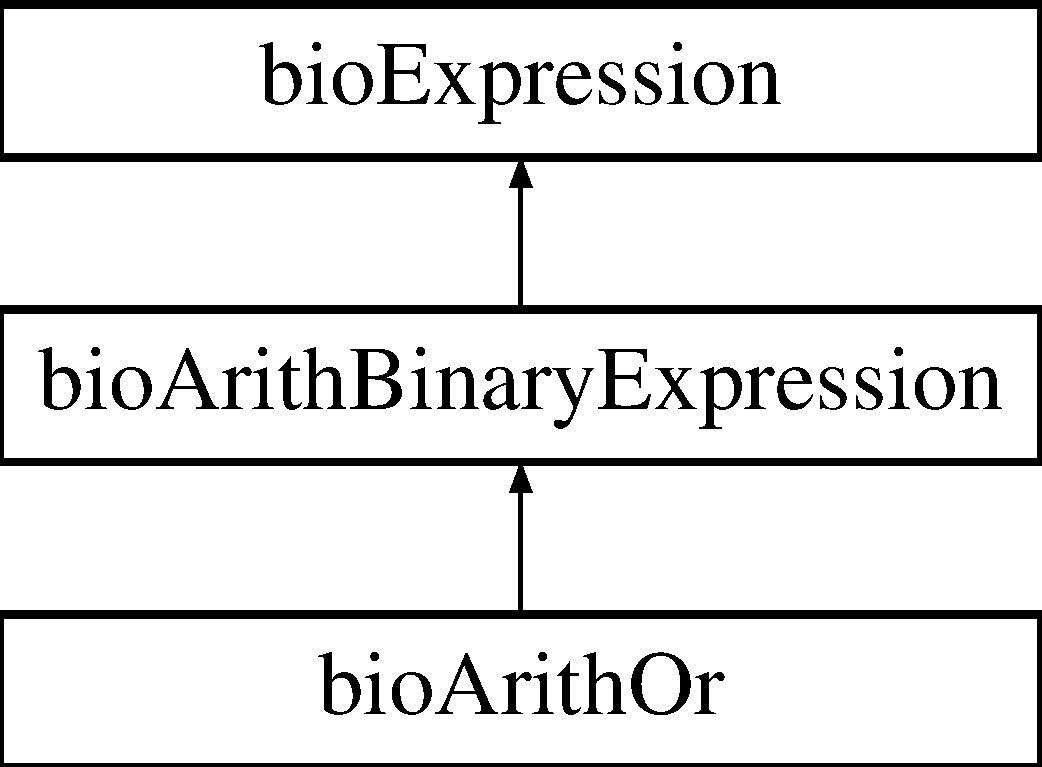
\includegraphics[height=3.000000cm]{classbio_arith_or}
\end{center}
\end{figure}
\subsection*{Public Member Functions}
\begin{DoxyCompactItemize}
\item 
\mbox{\Hypertarget{classbio_arith_or_a561f0b992c42bd8a634e5853d23fc172}\label{classbio_arith_or_a561f0b992c42bd8a634e5853d23fc172}} 
{\bfseries bio\+Arith\+Or} (\hyperlink{classbio_expression_repository}{bio\+Expression\+Repository} $\ast$rep, pat\+U\+Long par, pat\+U\+Long left, pat\+U\+Long right, pat\+Error $\ast$\&err)
\item 
virtual pat\+String \hyperlink{classbio_arith_or_afa8b3b4494ff72cdbbfda2012c56dc68}{get\+Operator\+Name} () const
\item 
virtual pat\+Real \hyperlink{classbio_arith_or_a59ec27e29f35c91f0a5fd2a8993a363b}{get\+Value} (pat\+Boolean prepare\+Gradient, pat\+U\+Long current\+Lap, pat\+Error $\ast$\&err)
\item 
virtual \hyperlink{classbio_expression}{bio\+Expression} $\ast$ \hyperlink{classbio_arith_or_a25b8deace8face416cb0cc711799506d}{get\+Derivative} (pat\+U\+Long a\+Literal\+Id, pat\+Error $\ast$\&err) const
\item 
virtual \hyperlink{classbio_arith_or}{bio\+Arith\+Or} $\ast$ \hyperlink{classbio_arith_or_aad2095426058f90fbb4acaa4ec9bf9fb}{get\+Deep\+Copy} (\hyperlink{classbio_expression_repository}{bio\+Expression\+Repository} $\ast$rep, pat\+Error $\ast$\&err) const
\item 
virtual \hyperlink{classbio_arith_or}{bio\+Arith\+Or} $\ast$ \hyperlink{classbio_arith_or_a64c0b100e6bc8d877bd25dbf5224ff0b}{get\+Shallow\+Copy} (\hyperlink{classbio_expression_repository}{bio\+Expression\+Repository} $\ast$rep, pat\+Error $\ast$\&err) const
\item 
virtual pat\+String \hyperlink{classbio_arith_or_aa31f4d5e3b2ac7df4c52b55f51819589}{get\+Expression\+String} () const
\item 
virtual \hyperlink{classbio_function_and_derivatives}{bio\+Function\+And\+Derivatives} $\ast$ \hyperlink{classbio_arith_or_a584c8a964a188ca03db9cf69400af290}{get\+Numerical\+Function\+And\+Gradient} (vector$<$ pat\+U\+Long $>$ literal\+Ids, pat\+Boolean compute\+Hessian, pat\+Boolean debug\+Derivatives, pat\+Error $\ast$\&err)
\end{DoxyCompactItemize}
\subsection*{Additional Inherited Members}


\subsection{Detailed Description}
Class implementing a node of the tree representing a logical or operation 

\subsection{Member Function Documentation}
\mbox{\Hypertarget{classbio_arith_or_aad2095426058f90fbb4acaa4ec9bf9fb}\label{classbio_arith_or_aad2095426058f90fbb4acaa4ec9bf9fb}} 
\index{bio\+Arith\+Or@{bio\+Arith\+Or}!get\+Deep\+Copy@{get\+Deep\+Copy}}
\index{get\+Deep\+Copy@{get\+Deep\+Copy}!bio\+Arith\+Or@{bio\+Arith\+Or}}
\subsubsection{\texorpdfstring{get\+Deep\+Copy()}{getDeepCopy()}}
{\footnotesize\ttfamily \hyperlink{classbio_arith_or}{bio\+Arith\+Or} $\ast$ bio\+Arith\+Or\+::get\+Deep\+Copy (\begin{DoxyParamCaption}\item[{\hyperlink{classbio_expression_repository}{bio\+Expression\+Repository} $\ast$}]{rep,  }\item[{pat\+Error $\ast$\&}]{err }\end{DoxyParamCaption}) const\hspace{0.3cm}{\ttfamily [virtual]}}

Create a deep copy of the expression and returns a pointer to it. It means that new instances of the children are created. 

Reimplemented from \hyperlink{classbio_expression_a4ee1b8add634078a02eaae26cd40dcc8}{bio\+Expression}.

\mbox{\Hypertarget{classbio_arith_or_a25b8deace8face416cb0cc711799506d}\label{classbio_arith_or_a25b8deace8face416cb0cc711799506d}} 
\index{bio\+Arith\+Or@{bio\+Arith\+Or}!get\+Derivative@{get\+Derivative}}
\index{get\+Derivative@{get\+Derivative}!bio\+Arith\+Or@{bio\+Arith\+Or}}
\subsubsection{\texorpdfstring{get\+Derivative()}{getDerivative()}}
{\footnotesize\ttfamily \hyperlink{classbio_expression}{bio\+Expression} $\ast$ bio\+Arith\+Or\+::get\+Derivative (\begin{DoxyParamCaption}\item[{pat\+U\+Long}]{a\+Literal\+Id,  }\item[{pat\+Error $\ast$\&}]{err }\end{DoxyParamCaption}) const\hspace{0.3cm}{\ttfamily [virtual]}}

\begin{DoxyReturn}{Returns}
value of the derivative w.\+r.\+t literal 
\end{DoxyReturn}

\begin{DoxyParams}{Parameters}
{\em index} & of the literal involved in the derivative \\
\hline
{\em err} & ref. of the pointer to the error object. \\
\hline
\end{DoxyParams}


Reimplemented from \hyperlink{classbio_expression_a5915579d1193f25f216c1e273c97f2ce}{bio\+Expression}.

\mbox{\Hypertarget{classbio_arith_or_aa31f4d5e3b2ac7df4c52b55f51819589}\label{classbio_arith_or_aa31f4d5e3b2ac7df4c52b55f51819589}} 
\index{bio\+Arith\+Or@{bio\+Arith\+Or}!get\+Expression\+String@{get\+Expression\+String}}
\index{get\+Expression\+String@{get\+Expression\+String}!bio\+Arith\+Or@{bio\+Arith\+Or}}
\subsubsection{\texorpdfstring{get\+Expression\+String()}{getExpressionString()}}
{\footnotesize\ttfamily pat\+String bio\+Arith\+Or\+::get\+Expression\+String (\begin{DoxyParamCaption}{ }\end{DoxyParamCaption}) const\hspace{0.3cm}{\ttfamily [virtual]}}

Compute a string that represents the expression. It is designed to replace the expression itself when used only for comparison purposes. Code\+: +\{expr1\}\{expr2\}\+: binary plus -\/\{expr1\}\{expr2\}\+: binary minus \{expr1\}\{expr2\}\+: multiplication /\{expr1\}\{expr2\}\+: division $^\wedge$\{expr1\}\{expr2\}\+: power \&\{expr1\}\{expr2\}\+: and $\vert$\{expr1\}\{expr2\}\+: or =\{expr1\}\{expr2\}\+: equal !=\{expr1\}\{expr2\}\+: not equal $<$\{expr1\}\{expr2\}\+: lesser than $<$=\{expr1\}\{expr2\}\+: lesser or equal to $>$\{expr1\}\{expr2\}\+: greater than $>$=\{expr1\}\{expr2\}\+: greater or equal to \$A\{expr\}\+: abs \$D\mbox{[}expr\mbox{]}\mbox{[}\{expr1\}...\{exprN\}\mbox{]}\+: dictionary (\hyperlink{classbio_arith_elem}{bio\+Arith\+Elem}) \$E\{expr\}\+: exp \$L\{expr\}\+: log \$M\{expr\}\+: Unary minus \$\+Piterator\+\_\+name\{expr\}\+: prod \$Q\{string1\}\{string2\}\+: sequence \$\+Siterator\+\_\+name\{expr\}\+: sum \$\+Ziterator\+\_\+name\mbox{[}\{expr1\}...\{exprN\}\mbox{]}\+: merged sum \{expr1\}\{expr2\}...\{exprN\}//\+: list of expressions number\+: constant \#id\+: literal \&id\+: random 

Reimplemented from \hyperlink{classbio_expression_a3e4b4dca58dbbc6f0e411b30eb3f60b4}{bio\+Expression}.

\mbox{\Hypertarget{classbio_arith_or_a584c8a964a188ca03db9cf69400af290}\label{classbio_arith_or_a584c8a964a188ca03db9cf69400af290}} 
\index{bio\+Arith\+Or@{bio\+Arith\+Or}!get\+Numerical\+Function\+And\+Gradient@{get\+Numerical\+Function\+And\+Gradient}}
\index{get\+Numerical\+Function\+And\+Gradient@{get\+Numerical\+Function\+And\+Gradient}!bio\+Arith\+Or@{bio\+Arith\+Or}}
\subsubsection{\texorpdfstring{get\+Numerical\+Function\+And\+Gradient()}{getNumericalFunctionAndGradient()}}
{\footnotesize\ttfamily \hyperlink{classbio_function_and_derivatives}{bio\+Function\+And\+Derivatives} $\ast$ bio\+Arith\+Or\+::get\+Numerical\+Function\+And\+Gradient (\begin{DoxyParamCaption}\item[{vector$<$ pat\+U\+Long $>$}]{literal\+Ids,  }\item[{pat\+Boolean}]{compute\+Hessian,  }\item[{pat\+Boolean}]{debug\+Derivatives,  }\item[{pat\+Error $\ast$\&}]{err }\end{DoxyParamCaption})\hspace{0.3cm}{\ttfamily [virtual]}}

\begin{DoxyReturn}{Returns}
value and gradient of the expression 
\end{DoxyReturn}

\begin{DoxyParams}{Parameters}
{\em err} & ref. of the pointer to the error object. \\
\hline
\end{DoxyParams}


Reimplemented from \hyperlink{classbio_expression_a91c81ce80c9e972c913b10f5f3c1ed13}{bio\+Expression}.

\mbox{\Hypertarget{classbio_arith_or_afa8b3b4494ff72cdbbfda2012c56dc68}\label{classbio_arith_or_afa8b3b4494ff72cdbbfda2012c56dc68}} 
\index{bio\+Arith\+Or@{bio\+Arith\+Or}!get\+Operator\+Name@{get\+Operator\+Name}}
\index{get\+Operator\+Name@{get\+Operator\+Name}!bio\+Arith\+Or@{bio\+Arith\+Or}}
\subsubsection{\texorpdfstring{get\+Operator\+Name()}{getOperatorName()}}
{\footnotesize\ttfamily pat\+String bio\+Arith\+Or\+::get\+Operator\+Name (\begin{DoxyParamCaption}{ }\end{DoxyParamCaption}) const\hspace{0.3cm}{\ttfamily [virtual]}}

\begin{DoxyReturn}{Returns}
name of the operator 
\end{DoxyReturn}


Reimplemented from \hyperlink{classbio_expression_a2353a4afb3a2b0af7c63aba086a72bde}{bio\+Expression}.

\mbox{\Hypertarget{classbio_arith_or_a64c0b100e6bc8d877bd25dbf5224ff0b}\label{classbio_arith_or_a64c0b100e6bc8d877bd25dbf5224ff0b}} 
\index{bio\+Arith\+Or@{bio\+Arith\+Or}!get\+Shallow\+Copy@{get\+Shallow\+Copy}}
\index{get\+Shallow\+Copy@{get\+Shallow\+Copy}!bio\+Arith\+Or@{bio\+Arith\+Or}}
\subsubsection{\texorpdfstring{get\+Shallow\+Copy()}{getShallowCopy()}}
{\footnotesize\ttfamily \hyperlink{classbio_arith_or}{bio\+Arith\+Or} $\ast$ bio\+Arith\+Or\+::get\+Shallow\+Copy (\begin{DoxyParamCaption}\item[{\hyperlink{classbio_expression_repository}{bio\+Expression\+Repository} $\ast$}]{rep,  }\item[{pat\+Error $\ast$\&}]{err }\end{DoxyParamCaption}) const\hspace{0.3cm}{\ttfamily [virtual]}}

Create a shallow copy of the expression and returns a pointer to it. It means that no new instance of the children are created. It is typically called by the repository 

Reimplemented from \hyperlink{classbio_expression_a442534762693b92baaf33928979a1bf8}{bio\+Expression}.

\mbox{\Hypertarget{classbio_arith_or_a59ec27e29f35c91f0a5fd2a8993a363b}\label{classbio_arith_or_a59ec27e29f35c91f0a5fd2a8993a363b}} 
\index{bio\+Arith\+Or@{bio\+Arith\+Or}!get\+Value@{get\+Value}}
\index{get\+Value@{get\+Value}!bio\+Arith\+Or@{bio\+Arith\+Or}}
\subsubsection{\texorpdfstring{get\+Value()}{getValue()}}
{\footnotesize\ttfamily pat\+Real bio\+Arith\+Or\+::get\+Value (\begin{DoxyParamCaption}\item[{pat\+Boolean}]{prepare\+Gradient,  }\item[{pat\+U\+Long}]{current\+Lap,  }\item[{pat\+Error $\ast$\&}]{err }\end{DoxyParamCaption})\hspace{0.3cm}{\ttfamily [virtual]}}

\begin{DoxyReturn}{Returns}
value of the expression 
\end{DoxyReturn}

\begin{DoxyParams}{Parameters}
{\em err} & ref. of the pointer to the error object. \\
\hline
\end{DoxyParams}


Reimplemented from \hyperlink{classbio_expression_af58662a5d4d456f15bc4f2c9bd4f8a5b}{bio\+Expression}.



The documentation for this class was generated from the following files\+:\begin{DoxyCompactItemize}
\item 
bio\+Arith\+Or.\+h\item 
bio\+Arith\+Or.\+cc\end{DoxyCompactItemize}

\hypertarget{classbio_arith_power}{}\section{bio\+Arith\+Power Class Reference}
\label{classbio_arith_power}\index{bio\+Arith\+Power@{bio\+Arith\+Power}}


{\ttfamily \#include $<$bio\+Arith\+Power.\+h$>$}

Inheritance diagram for bio\+Arith\+Power\+:\begin{figure}[H]
\begin{center}
\leavevmode
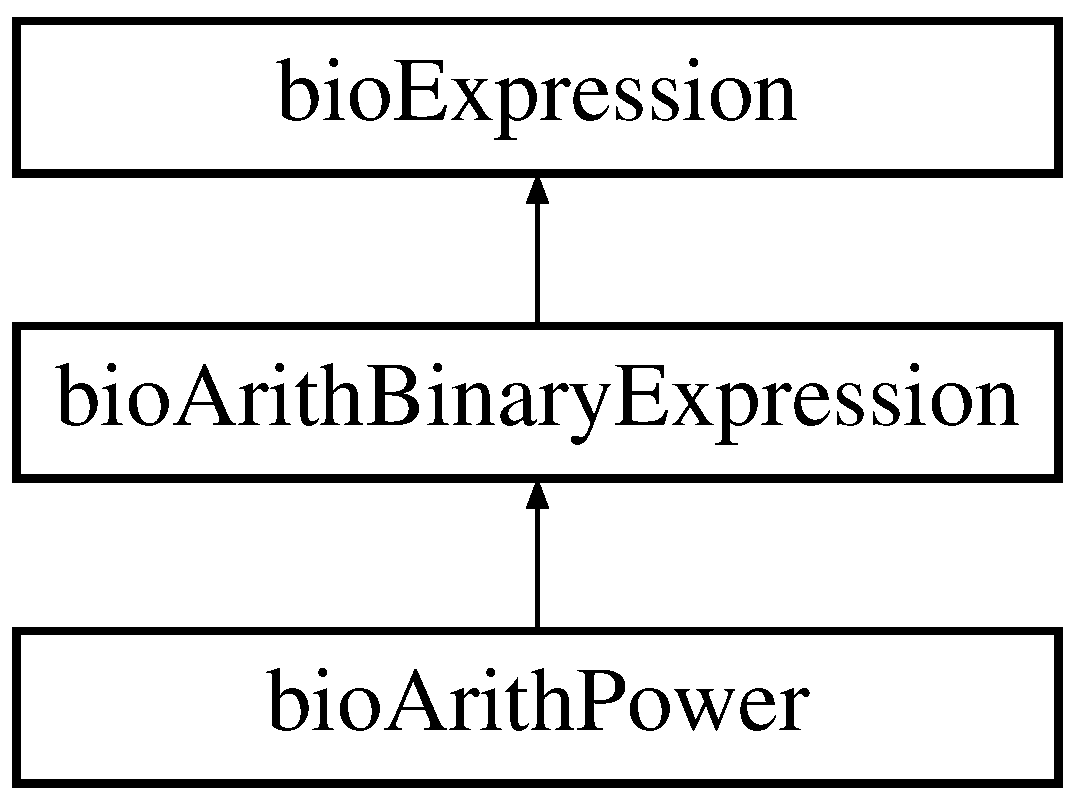
\includegraphics[height=3.000000cm]{classbio_arith_power}
\end{center}
\end{figure}
\subsection*{Public Member Functions}
\begin{DoxyCompactItemize}
\item 
\mbox{\Hypertarget{classbio_arith_power_ab5ce5ffc905627f20005fbf5d5c98575}\label{classbio_arith_power_ab5ce5ffc905627f20005fbf5d5c98575}} 
{\bfseries bio\+Arith\+Power} (\hyperlink{classbio_expression_repository}{bio\+Expression\+Repository} $\ast$rep, pat\+U\+Long par, pat\+U\+Long left, pat\+U\+Long right, pat\+Error $\ast$\&err)
\item 
virtual pat\+String \hyperlink{classbio_arith_power_a7edb8072b2c5aef093244305fbc76962}{get\+Operator\+Name} () const
\item 
virtual pat\+Real \hyperlink{classbio_arith_power_a3274071fcc8f58adb67b82880e178842}{get\+Value} (pat\+Boolean prepare\+Gradient, pat\+U\+Long current\+Lap, pat\+Error $\ast$\&err)
\item 
virtual \hyperlink{classbio_expression}{bio\+Expression} $\ast$ \hyperlink{classbio_arith_power_accc8e782d664f92db194ef1dc5a19e4b}{get\+Derivative} (pat\+U\+Long a\+Literal\+Id, pat\+Error $\ast$\&err) const
\item 
virtual \hyperlink{classbio_arith_power}{bio\+Arith\+Power} $\ast$ \hyperlink{classbio_arith_power_abad616d9928debfc78b8b8ecd1f0d9bd}{get\+Deep\+Copy} (\hyperlink{classbio_expression_repository}{bio\+Expression\+Repository} $\ast$rep, pat\+Error $\ast$\&err) const
\item 
virtual \hyperlink{classbio_arith_power}{bio\+Arith\+Power} $\ast$ \hyperlink{classbio_arith_power_a1a95ae563759a44ffb29b42c82209f90}{get\+Shallow\+Copy} (\hyperlink{classbio_expression_repository}{bio\+Expression\+Repository} $\ast$rep, pat\+Error $\ast$\&err) const
\item 
virtual pat\+Boolean \hyperlink{classbio_arith_power_a65021bc0ae804520ac1e64c665abc62a}{is\+Structurally\+Zero} () const
\item 
virtual pat\+String \hyperlink{classbio_arith_power_a90e7e9f398760b8c8f928ecfb7d7c3d3}{get\+Expression\+String} () const
\item 
virtual \hyperlink{classbio_function_and_derivatives}{bio\+Function\+And\+Derivatives} $\ast$ \hyperlink{classbio_arith_power_a21f939e2e8554c6ae153be6bdc873b1a}{get\+Numerical\+Function\+And\+Gradient} (vector$<$ pat\+U\+Long $>$ literal\+Ids, pat\+Boolean compute\+Hessian, pat\+Boolean debug\+Derivatives, pat\+Error $\ast$\&err)
\end{DoxyCompactItemize}
\subsection*{Additional Inherited Members}


\subsection{Detailed Description}
Class implementing a node of the tree representing a power operation 

\subsection{Member Function Documentation}
\mbox{\Hypertarget{classbio_arith_power_abad616d9928debfc78b8b8ecd1f0d9bd}\label{classbio_arith_power_abad616d9928debfc78b8b8ecd1f0d9bd}} 
\index{bio\+Arith\+Power@{bio\+Arith\+Power}!get\+Deep\+Copy@{get\+Deep\+Copy}}
\index{get\+Deep\+Copy@{get\+Deep\+Copy}!bio\+Arith\+Power@{bio\+Arith\+Power}}
\subsubsection{\texorpdfstring{get\+Deep\+Copy()}{getDeepCopy()}}
{\footnotesize\ttfamily \hyperlink{classbio_arith_power}{bio\+Arith\+Power} $\ast$ bio\+Arith\+Power\+::get\+Deep\+Copy (\begin{DoxyParamCaption}\item[{\hyperlink{classbio_expression_repository}{bio\+Expression\+Repository} $\ast$}]{rep,  }\item[{pat\+Error $\ast$\&}]{err }\end{DoxyParamCaption}) const\hspace{0.3cm}{\ttfamily [virtual]}}

Create a deep copy of the expression and returns a pointer to it. It means that new instances of the children are created. 

Reimplemented from \hyperlink{classbio_expression_a4ee1b8add634078a02eaae26cd40dcc8}{bio\+Expression}.

\mbox{\Hypertarget{classbio_arith_power_accc8e782d664f92db194ef1dc5a19e4b}\label{classbio_arith_power_accc8e782d664f92db194ef1dc5a19e4b}} 
\index{bio\+Arith\+Power@{bio\+Arith\+Power}!get\+Derivative@{get\+Derivative}}
\index{get\+Derivative@{get\+Derivative}!bio\+Arith\+Power@{bio\+Arith\+Power}}
\subsubsection{\texorpdfstring{get\+Derivative()}{getDerivative()}}
{\footnotesize\ttfamily \hyperlink{classbio_expression}{bio\+Expression} $\ast$ bio\+Arith\+Power\+::get\+Derivative (\begin{DoxyParamCaption}\item[{pat\+U\+Long}]{a\+Literal\+Id,  }\item[{pat\+Error $\ast$\&}]{err }\end{DoxyParamCaption}) const\hspace{0.3cm}{\ttfamily [virtual]}}

\begin{DoxyReturn}{Returns}
value of the derivative w.\+r.\+t literal 
\end{DoxyReturn}

\begin{DoxyParams}{Parameters}
{\em index} & of the literal involved in the derivative \\
\hline
{\em err} & ref. of the pointer to the error object. \\
\hline
\end{DoxyParams}


Reimplemented from \hyperlink{classbio_expression_a5915579d1193f25f216c1e273c97f2ce}{bio\+Expression}.

\mbox{\Hypertarget{classbio_arith_power_a90e7e9f398760b8c8f928ecfb7d7c3d3}\label{classbio_arith_power_a90e7e9f398760b8c8f928ecfb7d7c3d3}} 
\index{bio\+Arith\+Power@{bio\+Arith\+Power}!get\+Expression\+String@{get\+Expression\+String}}
\index{get\+Expression\+String@{get\+Expression\+String}!bio\+Arith\+Power@{bio\+Arith\+Power}}
\subsubsection{\texorpdfstring{get\+Expression\+String()}{getExpressionString()}}
{\footnotesize\ttfamily pat\+String bio\+Arith\+Power\+::get\+Expression\+String (\begin{DoxyParamCaption}{ }\end{DoxyParamCaption}) const\hspace{0.3cm}{\ttfamily [virtual]}}

Compute a string that represents the expression. It is designed to replace the expression itself when used only for comparison purposes. Code\+: +\{expr1\}\{expr2\}\+: binary plus -\/\{expr1\}\{expr2\}\+: binary minus \{expr1\}\{expr2\}\+: multiplication /\{expr1\}\{expr2\}\+: division $^\wedge$\{expr1\}\{expr2\}\+: power \&\{expr1\}\{expr2\}\+: and $\vert$\{expr1\}\{expr2\}\+: or =\{expr1\}\{expr2\}\+: equal !=\{expr1\}\{expr2\}\+: not equal $<$\{expr1\}\{expr2\}\+: lesser than $<$=\{expr1\}\{expr2\}\+: lesser or equal to $>$\{expr1\}\{expr2\}\+: greater than $>$=\{expr1\}\{expr2\}\+: greater or equal to \$A\{expr\}\+: abs \$D\mbox{[}expr\mbox{]}\mbox{[}\{expr1\}...\{exprN\}\mbox{]}\+: dictionary (\hyperlink{classbio_arith_elem}{bio\+Arith\+Elem}) \$E\{expr\}\+: exp \$L\{expr\}\+: log \$M\{expr\}\+: Unary minus \$\+Piterator\+\_\+name\{expr\}\+: prod \$Q\{string1\}\{string2\}\+: sequence \$\+Siterator\+\_\+name\{expr\}\+: sum \$\+Ziterator\+\_\+name\mbox{[}\{expr1\}...\{exprN\}\mbox{]}\+: merged sum \{expr1\}\{expr2\}...\{exprN\}//\+: list of expressions number\+: constant \#id\+: literal \&id\+: random 

Reimplemented from \hyperlink{classbio_expression_a3e4b4dca58dbbc6f0e411b30eb3f60b4}{bio\+Expression}.

\mbox{\Hypertarget{classbio_arith_power_a21f939e2e8554c6ae153be6bdc873b1a}\label{classbio_arith_power_a21f939e2e8554c6ae153be6bdc873b1a}} 
\index{bio\+Arith\+Power@{bio\+Arith\+Power}!get\+Numerical\+Function\+And\+Gradient@{get\+Numerical\+Function\+And\+Gradient}}
\index{get\+Numerical\+Function\+And\+Gradient@{get\+Numerical\+Function\+And\+Gradient}!bio\+Arith\+Power@{bio\+Arith\+Power}}
\subsubsection{\texorpdfstring{get\+Numerical\+Function\+And\+Gradient()}{getNumericalFunctionAndGradient()}}
{\footnotesize\ttfamily \hyperlink{classbio_function_and_derivatives}{bio\+Function\+And\+Derivatives} $\ast$ bio\+Arith\+Power\+::get\+Numerical\+Function\+And\+Gradient (\begin{DoxyParamCaption}\item[{vector$<$ pat\+U\+Long $>$}]{literal\+Ids,  }\item[{pat\+Boolean}]{compute\+Hessian,  }\item[{pat\+Boolean}]{debug\+Derivatives,  }\item[{pat\+Error $\ast$\&}]{err }\end{DoxyParamCaption})\hspace{0.3cm}{\ttfamily [virtual]}}

\begin{DoxyReturn}{Returns}
value and gradient of the expression 
\end{DoxyReturn}

\begin{DoxyParams}{Parameters}
{\em err} & ref. of the pointer to the error object. \\
\hline
\end{DoxyParams}


Reimplemented from \hyperlink{classbio_expression_a91c81ce80c9e972c913b10f5f3c1ed13}{bio\+Expression}.

\mbox{\Hypertarget{classbio_arith_power_a7edb8072b2c5aef093244305fbc76962}\label{classbio_arith_power_a7edb8072b2c5aef093244305fbc76962}} 
\index{bio\+Arith\+Power@{bio\+Arith\+Power}!get\+Operator\+Name@{get\+Operator\+Name}}
\index{get\+Operator\+Name@{get\+Operator\+Name}!bio\+Arith\+Power@{bio\+Arith\+Power}}
\subsubsection{\texorpdfstring{get\+Operator\+Name()}{getOperatorName()}}
{\footnotesize\ttfamily pat\+String bio\+Arith\+Power\+::get\+Operator\+Name (\begin{DoxyParamCaption}{ }\end{DoxyParamCaption}) const\hspace{0.3cm}{\ttfamily [virtual]}}

\begin{DoxyReturn}{Returns}
name of the operator 
\end{DoxyReturn}


Reimplemented from \hyperlink{classbio_expression_a2353a4afb3a2b0af7c63aba086a72bde}{bio\+Expression}.

\mbox{\Hypertarget{classbio_arith_power_a1a95ae563759a44ffb29b42c82209f90}\label{classbio_arith_power_a1a95ae563759a44ffb29b42c82209f90}} 
\index{bio\+Arith\+Power@{bio\+Arith\+Power}!get\+Shallow\+Copy@{get\+Shallow\+Copy}}
\index{get\+Shallow\+Copy@{get\+Shallow\+Copy}!bio\+Arith\+Power@{bio\+Arith\+Power}}
\subsubsection{\texorpdfstring{get\+Shallow\+Copy()}{getShallowCopy()}}
{\footnotesize\ttfamily \hyperlink{classbio_arith_power}{bio\+Arith\+Power} $\ast$ bio\+Arith\+Power\+::get\+Shallow\+Copy (\begin{DoxyParamCaption}\item[{\hyperlink{classbio_expression_repository}{bio\+Expression\+Repository} $\ast$}]{rep,  }\item[{pat\+Error $\ast$\&}]{err }\end{DoxyParamCaption}) const\hspace{0.3cm}{\ttfamily [virtual]}}

Create a shallow copy of the expression and returns a pointer to it. It means that no new instance of the children are created. It is typically called by the repository 

Reimplemented from \hyperlink{classbio_expression_a442534762693b92baaf33928979a1bf8}{bio\+Expression}.

\mbox{\Hypertarget{classbio_arith_power_a3274071fcc8f58adb67b82880e178842}\label{classbio_arith_power_a3274071fcc8f58adb67b82880e178842}} 
\index{bio\+Arith\+Power@{bio\+Arith\+Power}!get\+Value@{get\+Value}}
\index{get\+Value@{get\+Value}!bio\+Arith\+Power@{bio\+Arith\+Power}}
\subsubsection{\texorpdfstring{get\+Value()}{getValue()}}
{\footnotesize\ttfamily pat\+Real bio\+Arith\+Power\+::get\+Value (\begin{DoxyParamCaption}\item[{pat\+Boolean}]{prepare\+Gradient,  }\item[{pat\+U\+Long}]{current\+Lap,  }\item[{pat\+Error $\ast$\&}]{err }\end{DoxyParamCaption})\hspace{0.3cm}{\ttfamily [virtual]}}

\begin{DoxyReturn}{Returns}
value of the expression 
\end{DoxyReturn}

\begin{DoxyParams}{Parameters}
{\em err} & ref. of the pointer to the error object. \\
\hline
\end{DoxyParams}


Reimplemented from \hyperlink{classbio_expression_af58662a5d4d456f15bc4f2c9bd4f8a5b}{bio\+Expression}.

\mbox{\Hypertarget{classbio_arith_power_a65021bc0ae804520ac1e64c665abc62a}\label{classbio_arith_power_a65021bc0ae804520ac1e64c665abc62a}} 
\index{bio\+Arith\+Power@{bio\+Arith\+Power}!is\+Structurally\+Zero@{is\+Structurally\+Zero}}
\index{is\+Structurally\+Zero@{is\+Structurally\+Zero}!bio\+Arith\+Power@{bio\+Arith\+Power}}
\subsubsection{\texorpdfstring{is\+Structurally\+Zero()}{isStructurallyZero()}}
{\footnotesize\ttfamily pat\+Boolean bio\+Arith\+Power\+::is\+Structurally\+Zero (\begin{DoxyParamCaption}{ }\end{DoxyParamCaption}) const\hspace{0.3cm}{\ttfamily [virtual]}}

return pat\+T\+R\+UE if the expression is structurally 0 so that there is no need to evaluate it. In the base class, it return pat\+F\+A\+L\+SE. 

Reimplemented from \hyperlink{classbio_expression_a264c6d78671610ada8261d698e4c4c42}{bio\+Expression}.



The documentation for this class was generated from the following files\+:\begin{DoxyCompactItemize}
\item 
bio\+Arith\+Power.\+h\item 
bio\+Arith\+Power.\+cc\end{DoxyCompactItemize}

\hypertarget{classbio_arith_print}{}\section{bio\+Arith\+Print Class Reference}
\label{classbio_arith_print}\index{bio\+Arith\+Print@{bio\+Arith\+Print}}


{\ttfamily \#include $<$bio\+Arith\+Print.\+h$>$}

Inheritance diagram for bio\+Arith\+Print\+:\begin{figure}[H]
\begin{center}
\leavevmode
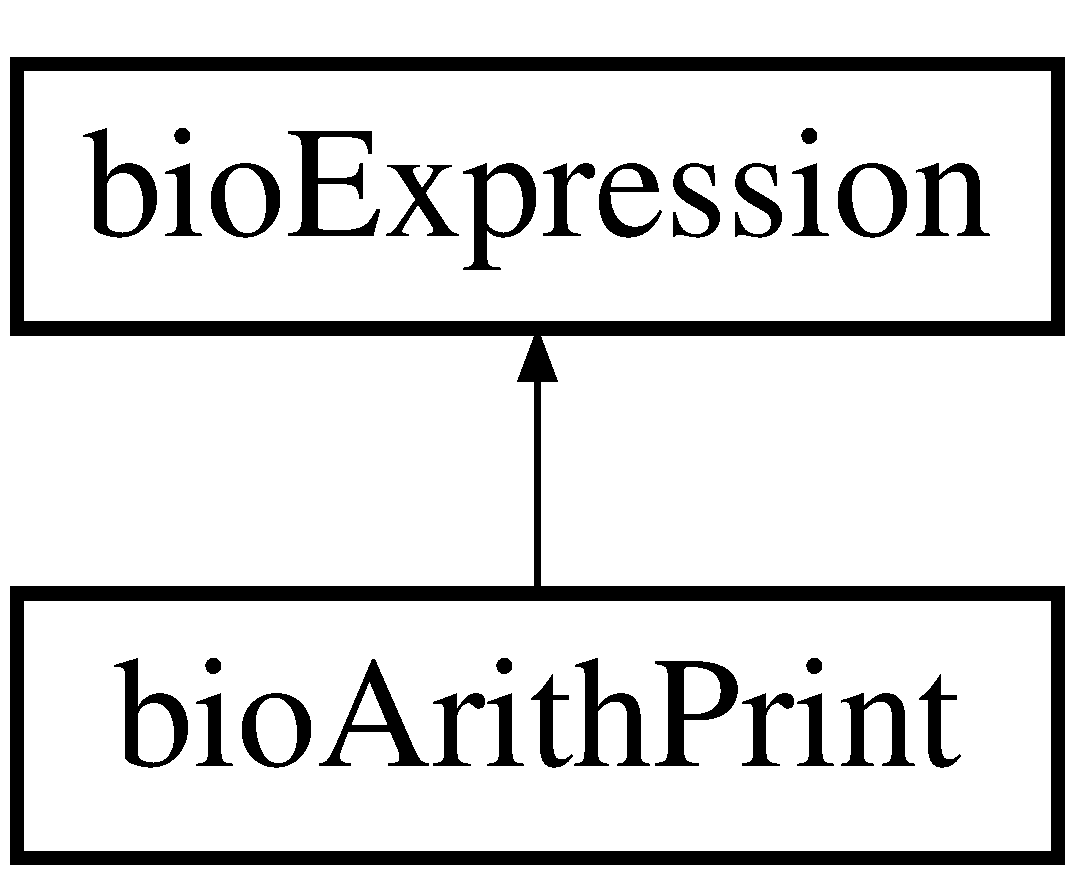
\includegraphics[height=2.000000cm]{classbio_arith_print}
\end{center}
\end{figure}
\subsection*{Public Member Functions}
\begin{DoxyCompactItemize}
\item 
\mbox{\Hypertarget{classbio_arith_print_aa2f7e9266af70a5b607230b4e0dd78ec}\label{classbio_arith_print_aa2f7e9266af70a5b607230b4e0dd78ec}} 
{\bfseries bio\+Arith\+Print} (\hyperlink{classbio_expression_repository}{bio\+Expression\+Repository} $\ast$rep, pat\+U\+Long par, map$<$ pat\+String, pat\+U\+Long $>$ the\+Terms, pat\+String an\+Iterator, pat\+Error $\ast$\&err)
\item 
virtual \hyperlink{classbio_expression}{bio\+Expression} $\ast$ \hyperlink{classbio_arith_print_aa9f08ee87d538bb2c90497e4b50948e1}{get\+Derivative} (pat\+U\+Long a\+Literal\+Id, pat\+Error $\ast$\&err) const
\item 
\mbox{\Hypertarget{classbio_arith_print_a33e4389d3563147e92ec8c94d6e40be6}\label{classbio_arith_print_a33e4389d3563147e92ec8c94d6e40be6}} 
virtual pat\+Boolean {\bfseries is\+Sum} () const
\item 
\mbox{\Hypertarget{classbio_arith_print_a2111fdbb86d2f43256bd9ba84eba9058}\label{classbio_arith_print_a2111fdbb86d2f43256bd9ba84eba9058}} 
virtual pat\+Boolean {\bfseries is\+Prod} () const
\item 
\mbox{\Hypertarget{classbio_arith_print_a3ba4d45966f3de4a2902c113ab3ea7a5}\label{classbio_arith_print_a3ba4d45966f3de4a2902c113ab3ea7a5}} 
virtual pat\+Boolean {\bfseries is\+Simulator} () const
\item 
\mbox{\Hypertarget{classbio_arith_print_a7ef938277148a1bc28d473a19a5ec624}\label{classbio_arith_print_a7ef938277148a1bc28d473a19a5ec624}} 
void {\bfseries simulate} (pat\+Hybrid\+Matrix $\ast$var\+Covar, vector$<$ pat\+String $>$ beta\+Names, \hyperlink{classbio_expression}{bio\+Expression} $\ast$weight, pat\+Error $\ast$\&err)
\item 
virtual pat\+String \hyperlink{classbio_arith_print_a7799066d3d3f68a685c89f46025f5aa8}{get\+Expression} (pat\+Error $\ast$\&err) const
\item 
virtual pat\+String \hyperlink{classbio_arith_print_a9451ac16baf5f060beafb2addb54a71e}{get\+Operator\+Name} () const
\item 
virtual pat\+Real \hyperlink{classbio_arith_print_a6c49bec841cdebd07ae234896c6d5416}{get\+Value} (pat\+Boolean prepare\+Gradient, pat\+U\+Long current\+Lap, pat\+Error $\ast$\&err)
\item 
virtual \hyperlink{classbio_arith_print}{bio\+Arith\+Print} $\ast$ \hyperlink{classbio_arith_print_a1a04e77640bd147c7a10d450d779ef1b}{get\+Deep\+Copy} (\hyperlink{classbio_expression_repository}{bio\+Expression\+Repository} $\ast$rep, pat\+Error $\ast$\&err) const
\item 
virtual \hyperlink{classbio_arith_print}{bio\+Arith\+Print} $\ast$ \hyperlink{classbio_arith_print_ac6387b4dbe1741adbc9343cef406b0c0}{get\+Shallow\+Copy} (\hyperlink{classbio_expression_repository}{bio\+Expression\+Repository} $\ast$rep, pat\+Error $\ast$\&err) const
\item 
virtual pat\+String \hyperlink{classbio_arith_print_ac850d47bf3a4d8dcf10d4b943a325103}{get\+Expression\+String} () const
\item 
\mbox{\Hypertarget{classbio_arith_print_aa43bcf71033b8d7e1ebdbc848b35d5d1}\label{classbio_arith_print_aa43bcf71033b8d7e1ebdbc848b35d5d1}} 
virtual pat\+U\+Long {\bfseries get\+Number\+Of\+Operations} () const
\item 
virtual \hyperlink{classbio_function_and_derivatives}{bio\+Function\+And\+Derivatives} $\ast$ \hyperlink{classbio_arith_print_a22180a362c2407a7941b465598981e96}{get\+Numerical\+Function\+And\+Gradient} (vector$<$ pat\+U\+Long $>$ literal\+Ids, pat\+Boolean compute\+Hessian, pat\+Boolean debug\+Derivatives, pat\+Error $\ast$\&err)
\item 
\mbox{\Hypertarget{classbio_arith_print_abe786c303fcb2ccc921e492c0de4cc34}\label{classbio_arith_print_abe786c303fcb2ccc921e492c0de4cc34}} 
virtual pat\+Boolean {\bfseries depends\+Of} (pat\+U\+Long a\+Literal\+Id) const
\item 
\mbox{\Hypertarget{classbio_arith_print_a13d857f722bf5aeb3b418e2417387eae}\label{classbio_arith_print_a13d857f722bf5aeb3b418e2417387eae}} 
virtual pat\+Boolean {\bfseries contains\+An\+Iterator} () const
\item 
\mbox{\Hypertarget{classbio_arith_print_ab4408176c0cb2d66a20d08ef6ca7ca2c}\label{classbio_arith_print_ab4408176c0cb2d66a20d08ef6ca7ca2c}} 
virtual pat\+Boolean {\bfseries contains\+An\+Iterator\+On\+Rows} () const
\item 
\mbox{\Hypertarget{classbio_arith_print_ac89f15c6ecee778da12604c2c31b1ae4}\label{classbio_arith_print_ac89f15c6ecee778da12604c2c31b1ae4}} 
virtual pat\+Boolean {\bfseries contains\+An\+Integral} () const
\item 
\mbox{\Hypertarget{classbio_arith_print_a8756a0405faa4e47236ddebd6ffcb561}\label{classbio_arith_print_a8756a0405faa4e47236ddebd6ffcb561}} 
virtual pat\+Boolean {\bfseries contains\+A\+Sequence} () const
\item 
\mbox{\Hypertarget{classbio_arith_print_a6dd938822f23961c70730837a87fd385}\label{classbio_arith_print_a6dd938822f23961c70730837a87fd385}} 
virtual pat\+String {\bfseries get\+Include\+Statements} (pat\+String prefix) const
\item 
\mbox{\Hypertarget{classbio_arith_print_adb79fc0f7bca600e0371c3056588f13e}\label{classbio_arith_print_adb79fc0f7bca600e0371c3056588f13e}} 
virtual void {\bfseries simplify\+Zeros} (pat\+Error $\ast$\&err)
\item 
\mbox{\Hypertarget{classbio_arith_print_ad0cadb289e58e7035ce22b9732a1a624}\label{classbio_arith_print_ad0cadb289e58e7035ce22b9732a1a624}} 
virtual void {\bfseries collect\+Expression\+Ids} (set$<$ pat\+U\+Long $>$ $\ast$s) const
\item 
\mbox{\Hypertarget{classbio_arith_print_ae6d141de8ae4526a438e58becc1cc1df}\label{classbio_arith_print_ae6d141de8ae4526a438e58becc1cc1df}} 
map$<$ pat\+String, \hyperlink{classbio_simulated_values}{bio\+Simulated\+Values} $>$ $\ast$ {\bfseries get\+Simulation\+Results} ()
\item 
\mbox{\Hypertarget{classbio_arith_print_adf09e74d63863554a7c7c1eaa53175f9}\label{classbio_arith_print_adf09e74d63863554a7c7c1eaa53175f9}} 
virtual pat\+String {\bfseries check} (pat\+Error $\ast$\&err) const
\end{DoxyCompactItemize}
\subsection*{Additional Inherited Members}


\subsection{Detailed Description}
Class implementing a node of the tree design to print the values of expressions 

\subsection{Member Function Documentation}
\mbox{\Hypertarget{classbio_arith_print_a1a04e77640bd147c7a10d450d779ef1b}\label{classbio_arith_print_a1a04e77640bd147c7a10d450d779ef1b}} 
\index{bio\+Arith\+Print@{bio\+Arith\+Print}!get\+Deep\+Copy@{get\+Deep\+Copy}}
\index{get\+Deep\+Copy@{get\+Deep\+Copy}!bio\+Arith\+Print@{bio\+Arith\+Print}}
\subsubsection{\texorpdfstring{get\+Deep\+Copy()}{getDeepCopy()}}
{\footnotesize\ttfamily \hyperlink{classbio_arith_print}{bio\+Arith\+Print} $\ast$ bio\+Arith\+Print\+::get\+Deep\+Copy (\begin{DoxyParamCaption}\item[{\hyperlink{classbio_expression_repository}{bio\+Expression\+Repository} $\ast$}]{rep,  }\item[{pat\+Error $\ast$\&}]{err }\end{DoxyParamCaption}) const\hspace{0.3cm}{\ttfamily [virtual]}}

Create a deep copy of the expression and returns a pointer to it. It means that new instances of the children are created. 

Reimplemented from \hyperlink{classbio_expression_a4ee1b8add634078a02eaae26cd40dcc8}{bio\+Expression}.

\mbox{\Hypertarget{classbio_arith_print_aa9f08ee87d538bb2c90497e4b50948e1}\label{classbio_arith_print_aa9f08ee87d538bb2c90497e4b50948e1}} 
\index{bio\+Arith\+Print@{bio\+Arith\+Print}!get\+Derivative@{get\+Derivative}}
\index{get\+Derivative@{get\+Derivative}!bio\+Arith\+Print@{bio\+Arith\+Print}}
\subsubsection{\texorpdfstring{get\+Derivative()}{getDerivative()}}
{\footnotesize\ttfamily \hyperlink{classbio_expression}{bio\+Expression} $\ast$ bio\+Arith\+Print\+::get\+Derivative (\begin{DoxyParamCaption}\item[{pat\+U\+Long}]{a\+Literal\+Id,  }\item[{pat\+Error $\ast$\&}]{err }\end{DoxyParamCaption}) const\hspace{0.3cm}{\ttfamily [virtual]}}

\begin{DoxyReturn}{Returns}
value of the derivative w.\+r.\+t literal 
\end{DoxyReturn}

\begin{DoxyParams}{Parameters}
{\em index} & of the literal involved in the derivative \\
\hline
{\em err} & ref. of the pointer to the error object. \\
\hline
\end{DoxyParams}


Reimplemented from \hyperlink{classbio_expression_a5915579d1193f25f216c1e273c97f2ce}{bio\+Expression}.

\mbox{\Hypertarget{classbio_arith_print_a7799066d3d3f68a685c89f46025f5aa8}\label{classbio_arith_print_a7799066d3d3f68a685c89f46025f5aa8}} 
\index{bio\+Arith\+Print@{bio\+Arith\+Print}!get\+Expression@{get\+Expression}}
\index{get\+Expression@{get\+Expression}!bio\+Arith\+Print@{bio\+Arith\+Print}}
\subsubsection{\texorpdfstring{get\+Expression()}{getExpression()}}
{\footnotesize\ttfamily pat\+String bio\+Arith\+Print\+::get\+Expression (\begin{DoxyParamCaption}\item[{pat\+Error $\ast$\&}]{err }\end{DoxyParamCaption}) const\hspace{0.3cm}{\ttfamily [virtual]}}

\begin{DoxyReturn}{Returns}
printed expression 
\end{DoxyReturn}


Reimplemented from \hyperlink{classbio_expression_a66a83eb0caac18dd5e568ffde5a8b5d4}{bio\+Expression}.

\mbox{\Hypertarget{classbio_arith_print_ac850d47bf3a4d8dcf10d4b943a325103}\label{classbio_arith_print_ac850d47bf3a4d8dcf10d4b943a325103}} 
\index{bio\+Arith\+Print@{bio\+Arith\+Print}!get\+Expression\+String@{get\+Expression\+String}}
\index{get\+Expression\+String@{get\+Expression\+String}!bio\+Arith\+Print@{bio\+Arith\+Print}}
\subsubsection{\texorpdfstring{get\+Expression\+String()}{getExpressionString()}}
{\footnotesize\ttfamily pat\+String bio\+Arith\+Print\+::get\+Expression\+String (\begin{DoxyParamCaption}{ }\end{DoxyParamCaption}) const\hspace{0.3cm}{\ttfamily [virtual]}}

Compute a string that represents the expression. It is designed to replace the expression itself when used only for comparison purposes. Code\+: +\{expr1\}\{expr2\}\+: binary plus -\/\{expr1\}\{expr2\}\+: binary minus \{expr1\}\{expr2\}\+: multiplication /\{expr1\}\{expr2\}\+: division $^\wedge$\{expr1\}\{expr2\}\+: power \&\{expr1\}\{expr2\}\+: and $\vert$\{expr1\}\{expr2\}\+: or =\{expr1\}\{expr2\}\+: equal !=\{expr1\}\{expr2\}\+: not equal $<$\{expr1\}\{expr2\}\+: lesser than $<$=\{expr1\}\{expr2\}\+: lesser or equal to $>$\{expr1\}\{expr2\}\+: greater than $>$=\{expr1\}\{expr2\}\+: greater or equal to \$A\{expr\}\+: abs \$D\mbox{[}expr\mbox{]}\mbox{[}\{expr1\}...\{exprN\}\mbox{]}\+: dictionary (\hyperlink{classbio_arith_elem}{bio\+Arith\+Elem}) \$E\{expr\}\+: exp \$L\{expr\}\+: log \$M\{expr\}\+: Unary minus \$\+Piterator\+\_\+name\{expr\}\+: prod \$Q\{string1\}\{string2\}\+: sequence \$\+Siterator\+\_\+name\{expr\}\+: sum \$\+Ziterator\+\_\+name\mbox{[}\{expr1\}...\{exprN\}\mbox{]}\+: merged sum \{expr1\}\{expr2\}...\{exprN\}//\+: list of expressions number\+: constant \#id\+: literal \&id\+: random 

Reimplemented from \hyperlink{classbio_expression_a3e4b4dca58dbbc6f0e411b30eb3f60b4}{bio\+Expression}.

\mbox{\Hypertarget{classbio_arith_print_a22180a362c2407a7941b465598981e96}\label{classbio_arith_print_a22180a362c2407a7941b465598981e96}} 
\index{bio\+Arith\+Print@{bio\+Arith\+Print}!get\+Numerical\+Function\+And\+Gradient@{get\+Numerical\+Function\+And\+Gradient}}
\index{get\+Numerical\+Function\+And\+Gradient@{get\+Numerical\+Function\+And\+Gradient}!bio\+Arith\+Print@{bio\+Arith\+Print}}
\subsubsection{\texorpdfstring{get\+Numerical\+Function\+And\+Gradient()}{getNumericalFunctionAndGradient()}}
{\footnotesize\ttfamily \hyperlink{classbio_function_and_derivatives}{bio\+Function\+And\+Derivatives} $\ast$ bio\+Arith\+Print\+::get\+Numerical\+Function\+And\+Gradient (\begin{DoxyParamCaption}\item[{vector$<$ pat\+U\+Long $>$}]{literal\+Ids,  }\item[{pat\+Boolean}]{compute\+Hessian,  }\item[{pat\+Boolean}]{debug\+Derivatives,  }\item[{pat\+Error $\ast$\&}]{err }\end{DoxyParamCaption})\hspace{0.3cm}{\ttfamily [virtual]}}

\begin{DoxyReturn}{Returns}
value and gradient of the expression 
\end{DoxyReturn}

\begin{DoxyParams}{Parameters}
{\em err} & ref. of the pointer to the error object. \\
\hline
\end{DoxyParams}


Reimplemented from \hyperlink{classbio_expression_a91c81ce80c9e972c913b10f5f3c1ed13}{bio\+Expression}.

\mbox{\Hypertarget{classbio_arith_print_a9451ac16baf5f060beafb2addb54a71e}\label{classbio_arith_print_a9451ac16baf5f060beafb2addb54a71e}} 
\index{bio\+Arith\+Print@{bio\+Arith\+Print}!get\+Operator\+Name@{get\+Operator\+Name}}
\index{get\+Operator\+Name@{get\+Operator\+Name}!bio\+Arith\+Print@{bio\+Arith\+Print}}
\subsubsection{\texorpdfstring{get\+Operator\+Name()}{getOperatorName()}}
{\footnotesize\ttfamily pat\+String bio\+Arith\+Print\+::get\+Operator\+Name (\begin{DoxyParamCaption}{ }\end{DoxyParamCaption}) const\hspace{0.3cm}{\ttfamily [virtual]}}

\begin{DoxyReturn}{Returns}
name of the operator 
\end{DoxyReturn}


Reimplemented from \hyperlink{classbio_expression_a2353a4afb3a2b0af7c63aba086a72bde}{bio\+Expression}.

\mbox{\Hypertarget{classbio_arith_print_ac6387b4dbe1741adbc9343cef406b0c0}\label{classbio_arith_print_ac6387b4dbe1741adbc9343cef406b0c0}} 
\index{bio\+Arith\+Print@{bio\+Arith\+Print}!get\+Shallow\+Copy@{get\+Shallow\+Copy}}
\index{get\+Shallow\+Copy@{get\+Shallow\+Copy}!bio\+Arith\+Print@{bio\+Arith\+Print}}
\subsubsection{\texorpdfstring{get\+Shallow\+Copy()}{getShallowCopy()}}
{\footnotesize\ttfamily \hyperlink{classbio_arith_print}{bio\+Arith\+Print} $\ast$ bio\+Arith\+Print\+::get\+Shallow\+Copy (\begin{DoxyParamCaption}\item[{\hyperlink{classbio_expression_repository}{bio\+Expression\+Repository} $\ast$}]{rep,  }\item[{pat\+Error $\ast$\&}]{err }\end{DoxyParamCaption}) const\hspace{0.3cm}{\ttfamily [virtual]}}

Create a shallow copy of the expression and returns a pointer to it. It means that no new instance of the children are created. It is typically called by the repository 

Reimplemented from \hyperlink{classbio_expression_a442534762693b92baaf33928979a1bf8}{bio\+Expression}.

\mbox{\Hypertarget{classbio_arith_print_a6c49bec841cdebd07ae234896c6d5416}\label{classbio_arith_print_a6c49bec841cdebd07ae234896c6d5416}} 
\index{bio\+Arith\+Print@{bio\+Arith\+Print}!get\+Value@{get\+Value}}
\index{get\+Value@{get\+Value}!bio\+Arith\+Print@{bio\+Arith\+Print}}
\subsubsection{\texorpdfstring{get\+Value()}{getValue()}}
{\footnotesize\ttfamily pat\+Real bio\+Arith\+Print\+::get\+Value (\begin{DoxyParamCaption}\item[{pat\+Boolean}]{prepare\+Gradient,  }\item[{pat\+U\+Long}]{current\+Lap,  }\item[{pat\+Error $\ast$\&}]{err }\end{DoxyParamCaption})\hspace{0.3cm}{\ttfamily [virtual]}}

\begin{DoxyReturn}{Returns}
value of the expression 
\end{DoxyReturn}

\begin{DoxyParams}{Parameters}
{\em err} & ref. of the pointer to the error object. \\
\hline
\end{DoxyParams}


Reimplemented from \hyperlink{classbio_expression_af58662a5d4d456f15bc4f2c9bd4f8a5b}{bio\+Expression}.



The documentation for this class was generated from the following files\+:\begin{DoxyCompactItemize}
\item 
bio\+Arith\+Print.\+h\item 
bio\+Arith\+Print.\+cc\end{DoxyCompactItemize}

\hypertarget{classbio_arith_prod}{}\section{bio\+Arith\+Prod Class Reference}
\label{classbio_arith_prod}\index{bio\+Arith\+Prod@{bio\+Arith\+Prod}}


{\ttfamily \#include $<$bio\+Arith\+Prod.\+h$>$}

Inheritance diagram for bio\+Arith\+Prod\+:\begin{figure}[H]
\begin{center}
\leavevmode
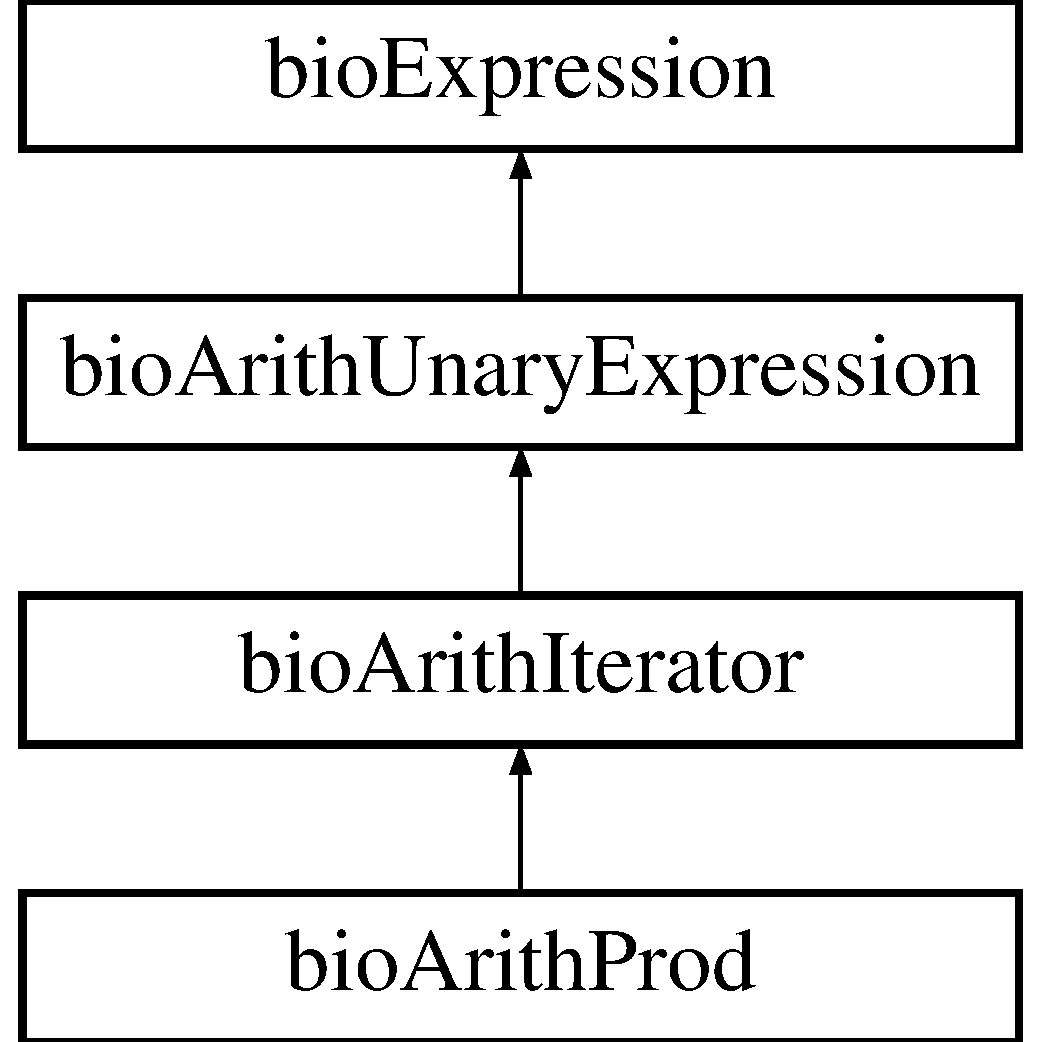
\includegraphics[height=4.000000cm]{classbio_arith_prod}
\end{center}
\end{figure}
\subsection*{Public Member Functions}
\begin{DoxyCompactItemize}
\item 
\mbox{\Hypertarget{classbio_arith_prod_a099b149adeaee35d97c8cf8be536187d}\label{classbio_arith_prod_a099b149adeaee35d97c8cf8be536187d}} 
{\bfseries bio\+Arith\+Prod} (\hyperlink{classbio_expression_repository}{bio\+Expression\+Repository} $\ast$rep, pat\+U\+Long par, pat\+U\+Long left, pat\+String an\+Iterator, pat\+Boolean is\+Positive, pat\+Error $\ast$\&err)
\item 
virtual pat\+String \hyperlink{classbio_arith_prod_a9157df784bda1e1ad425de27e05804b1}{get\+Operator\+Name} () const
\item 
virtual \hyperlink{classbio_expression}{bio\+Expression} $\ast$ \hyperlink{classbio_arith_prod_a1b086a865acfc23f3cd51566eaef8ddc}{get\+Derivative} (pat\+U\+Long a\+Literal\+Id, pat\+Error $\ast$\&err) const
\item 
virtual \hyperlink{classbio_arith_prod}{bio\+Arith\+Prod} $\ast$ \hyperlink{classbio_arith_prod_a55008811df00e22759086f4983362a26}{get\+Deep\+Copy} (\hyperlink{classbio_expression_repository}{bio\+Expression\+Repository} $\ast$rep, pat\+Error $\ast$\&err) const
\item 
virtual \hyperlink{classbio_arith_prod}{bio\+Arith\+Prod} $\ast$ \hyperlink{classbio_arith_prod_a8b4a3f836dc162ea067da896093c5f38}{get\+Shallow\+Copy} (\hyperlink{classbio_expression_repository}{bio\+Expression\+Repository} $\ast$rep, pat\+Error $\ast$\&err) const
\item 
\mbox{\Hypertarget{classbio_arith_prod_a87ccb533073f5f37f5eb19280275f2cb}\label{classbio_arith_prod_a87ccb533073f5f37f5eb19280275f2cb}} 
virtual pat\+Boolean {\bfseries is\+Sum} () const
\item 
\mbox{\Hypertarget{classbio_arith_prod_a41ee5a7a988ca881666825762aafdbe8}\label{classbio_arith_prod_a41ee5a7a988ca881666825762aafdbe8}} 
virtual pat\+Boolean {\bfseries is\+Prod} () const
\item 
virtual pat\+String \hyperlink{classbio_arith_prod_a665209a40bfb01098c5ddde204900294}{get\+Expression\+String} () const
\item 
virtual pat\+Real \hyperlink{classbio_arith_prod_a566bd383683dcd49930df1a1e5284918}{get\+Value} (pat\+Boolean prepare\+Gradient, pat\+U\+Long current\+Lap, pat\+Error $\ast$\&err)
\item 
\mbox{\Hypertarget{classbio_arith_prod_ab8151bb2d88725408d333b151961a5c7}\label{classbio_arith_prod_ab8151bb2d88725408d333b151961a5c7}} 
virtual pat\+U\+Long {\bfseries get\+Number\+Of\+Operations} () const
\item 
virtual \hyperlink{classbio_function_and_derivatives}{bio\+Function\+And\+Derivatives} $\ast$ \hyperlink{classbio_arith_prod_a6f7d57d9c0ec86aed9bb7eb643beb44e}{get\+Numerical\+Function\+And\+Gradient} (vector$<$ pat\+U\+Long $>$ literal\+Ids, pat\+Boolean compute\+Hessian, pat\+Boolean debug\+Derivatives, pat\+Error $\ast$\&err)
\end{DoxyCompactItemize}
\subsection*{Additional Inherited Members}


\subsection{Detailed Description}
Class implementing a node of the tree representing a product expression 

\subsection{Member Function Documentation}
\mbox{\Hypertarget{classbio_arith_prod_a55008811df00e22759086f4983362a26}\label{classbio_arith_prod_a55008811df00e22759086f4983362a26}} 
\index{bio\+Arith\+Prod@{bio\+Arith\+Prod}!get\+Deep\+Copy@{get\+Deep\+Copy}}
\index{get\+Deep\+Copy@{get\+Deep\+Copy}!bio\+Arith\+Prod@{bio\+Arith\+Prod}}
\subsubsection{\texorpdfstring{get\+Deep\+Copy()}{getDeepCopy()}}
{\footnotesize\ttfamily \hyperlink{classbio_arith_prod}{bio\+Arith\+Prod} $\ast$ bio\+Arith\+Prod\+::get\+Deep\+Copy (\begin{DoxyParamCaption}\item[{\hyperlink{classbio_expression_repository}{bio\+Expression\+Repository} $\ast$}]{rep,  }\item[{pat\+Error $\ast$\&}]{err }\end{DoxyParamCaption}) const\hspace{0.3cm}{\ttfamily [virtual]}}

Create a deep copy of the expression and returns a pointer to it. It means that new instances of the children are created. 

Reimplemented from \hyperlink{classbio_expression_a4ee1b8add634078a02eaae26cd40dcc8}{bio\+Expression}.

\mbox{\Hypertarget{classbio_arith_prod_a1b086a865acfc23f3cd51566eaef8ddc}\label{classbio_arith_prod_a1b086a865acfc23f3cd51566eaef8ddc}} 
\index{bio\+Arith\+Prod@{bio\+Arith\+Prod}!get\+Derivative@{get\+Derivative}}
\index{get\+Derivative@{get\+Derivative}!bio\+Arith\+Prod@{bio\+Arith\+Prod}}
\subsubsection{\texorpdfstring{get\+Derivative()}{getDerivative()}}
{\footnotesize\ttfamily \hyperlink{classbio_expression}{bio\+Expression} $\ast$ bio\+Arith\+Prod\+::get\+Derivative (\begin{DoxyParamCaption}\item[{pat\+U\+Long}]{a\+Literal\+Id,  }\item[{pat\+Error $\ast$\&}]{err }\end{DoxyParamCaption}) const\hspace{0.3cm}{\ttfamily [virtual]}}

\begin{DoxyReturn}{Returns}
value of the derivative w.\+r.\+t literal 
\end{DoxyReturn}

\begin{DoxyParams}{Parameters}
{\em index} & of the literal involved in the derivative \\
\hline
{\em err} & ref. of the pointer to the error object. \\
\hline
\end{DoxyParams}


Reimplemented from \hyperlink{classbio_expression_a5915579d1193f25f216c1e273c97f2ce}{bio\+Expression}.

\mbox{\Hypertarget{classbio_arith_prod_a665209a40bfb01098c5ddde204900294}\label{classbio_arith_prod_a665209a40bfb01098c5ddde204900294}} 
\index{bio\+Arith\+Prod@{bio\+Arith\+Prod}!get\+Expression\+String@{get\+Expression\+String}}
\index{get\+Expression\+String@{get\+Expression\+String}!bio\+Arith\+Prod@{bio\+Arith\+Prod}}
\subsubsection{\texorpdfstring{get\+Expression\+String()}{getExpressionString()}}
{\footnotesize\ttfamily pat\+String bio\+Arith\+Prod\+::get\+Expression\+String (\begin{DoxyParamCaption}{ }\end{DoxyParamCaption}) const\hspace{0.3cm}{\ttfamily [virtual]}}

Compute a string that represents the expression. It is designed to replace the expression itself when used only for comparison purposes. Code\+: +\{expr1\}\{expr2\}\+: binary plus -\/\{expr1\}\{expr2\}\+: binary minus \{expr1\}\{expr2\}\+: multiplication /\{expr1\}\{expr2\}\+: division $^\wedge$\{expr1\}\{expr2\}\+: power \&\{expr1\}\{expr2\}\+: and $\vert$\{expr1\}\{expr2\}\+: or =\{expr1\}\{expr2\}\+: equal !=\{expr1\}\{expr2\}\+: not equal $<$\{expr1\}\{expr2\}\+: lesser than $<$=\{expr1\}\{expr2\}\+: lesser or equal to $>$\{expr1\}\{expr2\}\+: greater than $>$=\{expr1\}\{expr2\}\+: greater or equal to \$A\{expr\}\+: abs \$D\mbox{[}expr\mbox{]}\mbox{[}\{expr1\}...\{exprN\}\mbox{]}\+: dictionary (\hyperlink{classbio_arith_elem}{bio\+Arith\+Elem}) \$E\{expr\}\+: exp \$L\{expr\}\+: log \$M\{expr\}\+: Unary minus \$\+Piterator\+\_\+name\{expr\}\+: prod \$Q\{string1\}\{string2\}\+: sequence \$\+Siterator\+\_\+name\{expr\}\+: sum \$\+Ziterator\+\_\+name\mbox{[}\{expr1\}...\{exprN\}\mbox{]}\+: merged sum \{expr1\}\{expr2\}...\{exprN\}//\+: list of expressions number\+: constant \#id\+: literal \&id\+: random 

Reimplemented from \hyperlink{classbio_expression_a3e4b4dca58dbbc6f0e411b30eb3f60b4}{bio\+Expression}.

\mbox{\Hypertarget{classbio_arith_prod_a6f7d57d9c0ec86aed9bb7eb643beb44e}\label{classbio_arith_prod_a6f7d57d9c0ec86aed9bb7eb643beb44e}} 
\index{bio\+Arith\+Prod@{bio\+Arith\+Prod}!get\+Numerical\+Function\+And\+Gradient@{get\+Numerical\+Function\+And\+Gradient}}
\index{get\+Numerical\+Function\+And\+Gradient@{get\+Numerical\+Function\+And\+Gradient}!bio\+Arith\+Prod@{bio\+Arith\+Prod}}
\subsubsection{\texorpdfstring{get\+Numerical\+Function\+And\+Gradient()}{getNumericalFunctionAndGradient()}}
{\footnotesize\ttfamily \hyperlink{classbio_function_and_derivatives}{bio\+Function\+And\+Derivatives} $\ast$ bio\+Arith\+Prod\+::get\+Numerical\+Function\+And\+Gradient (\begin{DoxyParamCaption}\item[{vector$<$ pat\+U\+Long $>$}]{literal\+Ids,  }\item[{pat\+Boolean}]{compute\+Hessian,  }\item[{pat\+Boolean}]{debug\+Derivatives,  }\item[{pat\+Error $\ast$\&}]{err }\end{DoxyParamCaption})\hspace{0.3cm}{\ttfamily [virtual]}}

\begin{DoxyReturn}{Returns}
value and gradient of the expression 
\end{DoxyReturn}

\begin{DoxyParams}{Parameters}
{\em err} & ref. of the pointer to the error object. \\
\hline
\end{DoxyParams}


Reimplemented from \hyperlink{classbio_expression_a91c81ce80c9e972c913b10f5f3c1ed13}{bio\+Expression}.

\mbox{\Hypertarget{classbio_arith_prod_a9157df784bda1e1ad425de27e05804b1}\label{classbio_arith_prod_a9157df784bda1e1ad425de27e05804b1}} 
\index{bio\+Arith\+Prod@{bio\+Arith\+Prod}!get\+Operator\+Name@{get\+Operator\+Name}}
\index{get\+Operator\+Name@{get\+Operator\+Name}!bio\+Arith\+Prod@{bio\+Arith\+Prod}}
\subsubsection{\texorpdfstring{get\+Operator\+Name()}{getOperatorName()}}
{\footnotesize\ttfamily pat\+String bio\+Arith\+Prod\+::get\+Operator\+Name (\begin{DoxyParamCaption}{ }\end{DoxyParamCaption}) const\hspace{0.3cm}{\ttfamily [virtual]}}

\begin{DoxyReturn}{Returns}
name of the operator 
\end{DoxyReturn}


Reimplemented from \hyperlink{classbio_expression_a2353a4afb3a2b0af7c63aba086a72bde}{bio\+Expression}.

\mbox{\Hypertarget{classbio_arith_prod_a8b4a3f836dc162ea067da896093c5f38}\label{classbio_arith_prod_a8b4a3f836dc162ea067da896093c5f38}} 
\index{bio\+Arith\+Prod@{bio\+Arith\+Prod}!get\+Shallow\+Copy@{get\+Shallow\+Copy}}
\index{get\+Shallow\+Copy@{get\+Shallow\+Copy}!bio\+Arith\+Prod@{bio\+Arith\+Prod}}
\subsubsection{\texorpdfstring{get\+Shallow\+Copy()}{getShallowCopy()}}
{\footnotesize\ttfamily \hyperlink{classbio_arith_prod}{bio\+Arith\+Prod} $\ast$ bio\+Arith\+Prod\+::get\+Shallow\+Copy (\begin{DoxyParamCaption}\item[{\hyperlink{classbio_expression_repository}{bio\+Expression\+Repository} $\ast$}]{rep,  }\item[{pat\+Error $\ast$\&}]{err }\end{DoxyParamCaption}) const\hspace{0.3cm}{\ttfamily [virtual]}}

Create a shallow copy of the expression and returns a pointer to it. It means that no new instance of the children are created. It is typically called by the repository 

Reimplemented from \hyperlink{classbio_expression_a442534762693b92baaf33928979a1bf8}{bio\+Expression}.

\mbox{\Hypertarget{classbio_arith_prod_a566bd383683dcd49930df1a1e5284918}\label{classbio_arith_prod_a566bd383683dcd49930df1a1e5284918}} 
\index{bio\+Arith\+Prod@{bio\+Arith\+Prod}!get\+Value@{get\+Value}}
\index{get\+Value@{get\+Value}!bio\+Arith\+Prod@{bio\+Arith\+Prod}}
\subsubsection{\texorpdfstring{get\+Value()}{getValue()}}
{\footnotesize\ttfamily pat\+Real bio\+Arith\+Prod\+::get\+Value (\begin{DoxyParamCaption}\item[{pat\+Boolean}]{prepare\+Gradient,  }\item[{pat\+U\+Long}]{current\+Lap,  }\item[{pat\+Error $\ast$\&}]{err }\end{DoxyParamCaption})\hspace{0.3cm}{\ttfamily [virtual]}}

\begin{DoxyReturn}{Returns}
value of the expression 
\end{DoxyReturn}

\begin{DoxyParams}{Parameters}
{\em err} & ref. of the pointer to the error object. \\
\hline
\end{DoxyParams}


Reimplemented from \hyperlink{classbio_expression_af58662a5d4d456f15bc4f2c9bd4f8a5b}{bio\+Expression}.



The documentation for this class was generated from the following files\+:\begin{DoxyCompactItemize}
\item 
bio\+Arith\+Prod.\+h\item 
bio\+Arith\+Prod.\+cc\end{DoxyCompactItemize}

\hypertarget{classbio_arith_random}{}\section{bio\+Arith\+Random Class Reference}
\label{classbio_arith_random}\index{bio\+Arith\+Random@{bio\+Arith\+Random}}


{\ttfamily \#include $<$bio\+Arith\+Random.\+h$>$}

Inheritance diagram for bio\+Arith\+Random\+:\begin{figure}[H]
\begin{center}
\leavevmode
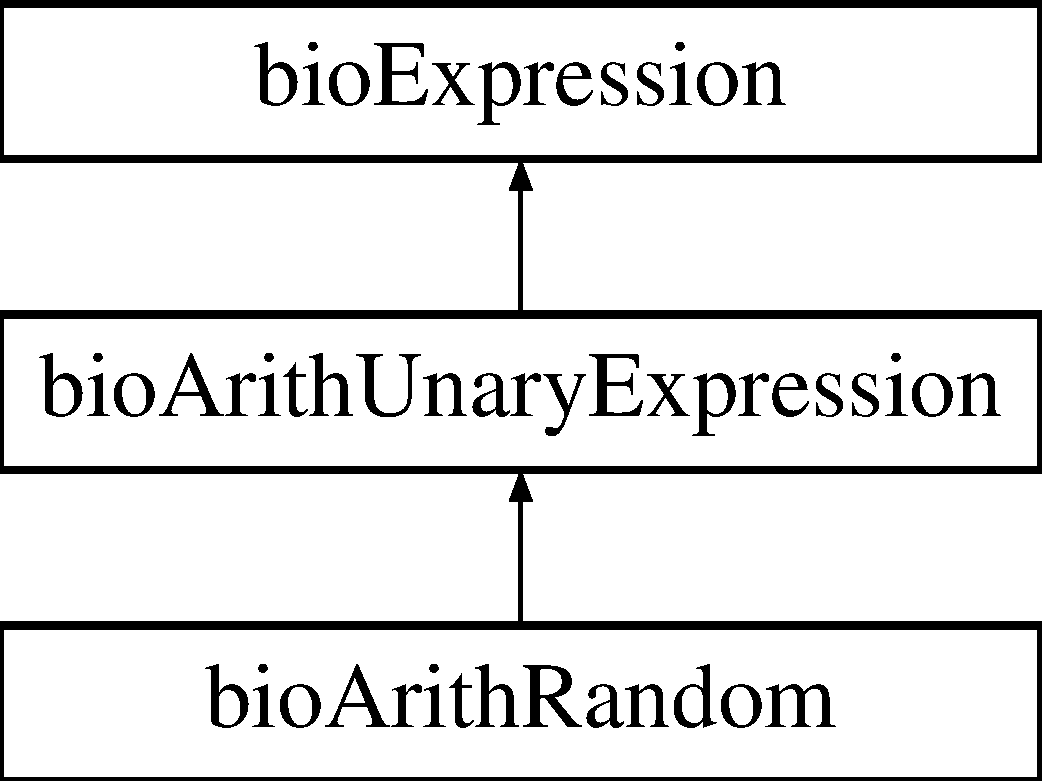
\includegraphics[height=3.000000cm]{classbio_arith_random}
\end{center}
\end{figure}
\subsection*{Public Member Functions}
\begin{DoxyCompactItemize}
\item 
\mbox{\Hypertarget{classbio_arith_random_a71bf8f6465482ac55bdaecf57091c09b}\label{classbio_arith_random_a71bf8f6465482ac55bdaecf57091c09b}} 
{\bfseries bio\+Arith\+Random} (\hyperlink{classbio_expression_repository}{bio\+Expression\+Repository} $\ast$rep, pat\+U\+Long par, pat\+U\+Long individual, pat\+U\+Long id, bio\+Random\+Draws\+::bio\+Draws\+Type type, pat\+Error $\ast$\&err)
\item 
pat\+String \hyperlink{classbio_arith_random_a0f83701f05a22956b5c4fff431c40895}{get\+Operator\+Name} () const
\item 
virtual pat\+Real \hyperlink{classbio_arith_random_a57ed5e619ea85ce7a4ece51ce4e05983}{get\+Value} (pat\+Boolean prepare\+Gradient, pat\+U\+Long current\+Lap, pat\+Error $\ast$\&err)
\item 
\hyperlink{classbio_expression}{bio\+Expression} $\ast$ \hyperlink{classbio_arith_random_a20b4fe8de86bf00654a94b0d534e6743}{get\+Derivative} (pat\+U\+Long a\+Literal\+Id, pat\+Error $\ast$\&err) const
\item 
\hyperlink{classbio_arith_random}{bio\+Arith\+Random} $\ast$ \hyperlink{classbio_arith_random_a947f100ddb8037bf424d343faee56b83}{get\+Deep\+Copy} (\hyperlink{classbio_expression_repository}{bio\+Expression\+Repository} $\ast$rep, pat\+Error $\ast$\&err) const
\item 
\hyperlink{classbio_arith_random}{bio\+Arith\+Random} $\ast$ \hyperlink{classbio_arith_random_aef00154ab54de9ed4acd1cf45d9036ce}{get\+Shallow\+Copy} (\hyperlink{classbio_expression_repository}{bio\+Expression\+Repository} $\ast$rep, pat\+Error $\ast$\&err) const
\item 
\mbox{\Hypertarget{classbio_arith_random_aeb2882becaab6950ee4582b750d80f35}\label{classbio_arith_random_aeb2882becaab6950ee4582b750d80f35}} 
pat\+U\+Long {\bfseries get\+Number\+Of\+Operations} () const
\item 
pat\+String \hyperlink{classbio_arith_random_a9ba191f0138f188b1c70f568c5873434}{get\+Expression\+String} () const
\item 
pat\+String \hyperlink{classbio_arith_random_a54b48a4876469d44f324f73758ea1b6c}{get\+Expression} (pat\+Error $\ast$\&err) const
\item 
\mbox{\Hypertarget{classbio_arith_random_a04107a0b2b42f92d6725c8871da676ca}\label{classbio_arith_random_a04107a0b2b42f92d6725c8871da676ca}} 
pat\+Boolean {\bfseries depends\+Of} (pat\+U\+Long a\+Literal\+Id) const
\item 
virtual \hyperlink{classbio_function_and_derivatives}{bio\+Function\+And\+Derivatives} $\ast$ \hyperlink{classbio_arith_random_a6f422273cd162e5d7d5e6d1d7a7ddcad}{get\+Numerical\+Function\+And\+Gradient} (vector$<$ pat\+U\+Long $>$ literal\+Ids, pat\+Boolean compute\+Hessian, pat\+Boolean debug\+Derivatives, pat\+Error $\ast$\&err)
\item 
\mbox{\Hypertarget{classbio_arith_random_aaeddba98a82767cc3d05b01904350acb}\label{classbio_arith_random_aaeddba98a82767cc3d05b01904350acb}} 
vector$<$ pat\+U\+Long $>$ {\bfseries get\+List\+Of\+Draws} (pat\+Error $\ast$\&err) const
\item 
\mbox{\Hypertarget{classbio_arith_random_aa6f751502c47dc7030fb451cc3317a4d}\label{classbio_arith_random_aa6f751502c47dc7030fb451cc3317a4d}} 
void {\bfseries check\+Monte\+Carlo} (pat\+Boolean inside\+Monte\+Carlo, pat\+Error $\ast$\&err)
\end{DoxyCompactItemize}
\subsection*{Protected Attributes}
\begin{DoxyCompactItemize}
\item 
\mbox{\Hypertarget{classbio_arith_random_a2370aa514ceefb3834a485daab8d8d9f}\label{classbio_arith_random_a2370aa514ceefb3834a485daab8d8d9f}} 
pat\+U\+Long {\bfseries variable\+Id\+For\+Draws}
\item 
\mbox{\Hypertarget{classbio_arith_random_ac09cba65919ec62338570a8a25994f0f}\label{classbio_arith_random_ac09cba65919ec62338570a8a25994f0f}} 
bio\+Random\+Draws\+::bio\+Draws\+Type {\bfseries type}
\end{DoxyCompactItemize}


\subsection{Detailed Description}
Class defining an interface for a random parameter uusing draws 

\subsection{Member Function Documentation}
\mbox{\Hypertarget{classbio_arith_random_a947f100ddb8037bf424d343faee56b83}\label{classbio_arith_random_a947f100ddb8037bf424d343faee56b83}} 
\index{bio\+Arith\+Random@{bio\+Arith\+Random}!get\+Deep\+Copy@{get\+Deep\+Copy}}
\index{get\+Deep\+Copy@{get\+Deep\+Copy}!bio\+Arith\+Random@{bio\+Arith\+Random}}
\subsubsection{\texorpdfstring{get\+Deep\+Copy()}{getDeepCopy()}}
{\footnotesize\ttfamily \hyperlink{classbio_arith_random}{bio\+Arith\+Random} $\ast$ bio\+Arith\+Random\+::get\+Deep\+Copy (\begin{DoxyParamCaption}\item[{\hyperlink{classbio_expression_repository}{bio\+Expression\+Repository} $\ast$}]{rep,  }\item[{pat\+Error $\ast$\&}]{err }\end{DoxyParamCaption}) const\hspace{0.3cm}{\ttfamily [virtual]}}

Create a deep copy of the expression and returns a pointer to it. It means that new instances of the children are created. 

Reimplemented from \hyperlink{classbio_expression_a4ee1b8add634078a02eaae26cd40dcc8}{bio\+Expression}.

\mbox{\Hypertarget{classbio_arith_random_a20b4fe8de86bf00654a94b0d534e6743}\label{classbio_arith_random_a20b4fe8de86bf00654a94b0d534e6743}} 
\index{bio\+Arith\+Random@{bio\+Arith\+Random}!get\+Derivative@{get\+Derivative}}
\index{get\+Derivative@{get\+Derivative}!bio\+Arith\+Random@{bio\+Arith\+Random}}
\subsubsection{\texorpdfstring{get\+Derivative()}{getDerivative()}}
{\footnotesize\ttfamily \hyperlink{classbio_expression}{bio\+Expression} $\ast$ bio\+Arith\+Random\+::get\+Derivative (\begin{DoxyParamCaption}\item[{pat\+U\+Long}]{a\+Literal\+Id,  }\item[{pat\+Error $\ast$\&}]{err }\end{DoxyParamCaption}) const\hspace{0.3cm}{\ttfamily [virtual]}}

\begin{DoxyReturn}{Returns}
value of the derivative w.\+r.\+t literal 
\end{DoxyReturn}

\begin{DoxyParams}{Parameters}
{\em index} & of the literal involved in the derivative \\
\hline
{\em err} & ref. of the pointer to the error object. \\
\hline
\end{DoxyParams}


Reimplemented from \hyperlink{classbio_expression_a5915579d1193f25f216c1e273c97f2ce}{bio\+Expression}.

\mbox{\Hypertarget{classbio_arith_random_a54b48a4876469d44f324f73758ea1b6c}\label{classbio_arith_random_a54b48a4876469d44f324f73758ea1b6c}} 
\index{bio\+Arith\+Random@{bio\+Arith\+Random}!get\+Expression@{get\+Expression}}
\index{get\+Expression@{get\+Expression}!bio\+Arith\+Random@{bio\+Arith\+Random}}
\subsubsection{\texorpdfstring{get\+Expression()}{getExpression()}}
{\footnotesize\ttfamily pat\+String bio\+Arith\+Random\+::get\+Expression (\begin{DoxyParamCaption}\item[{pat\+Error $\ast$\&}]{err }\end{DoxyParamCaption}) const\hspace{0.3cm}{\ttfamily [virtual]}}

\begin{DoxyReturn}{Returns}
printed expression 
\end{DoxyReturn}


Reimplemented from \hyperlink{classbio_arith_unary_expression_a974b7779804861f331a75e08db377926}{bio\+Arith\+Unary\+Expression}.

\mbox{\Hypertarget{classbio_arith_random_a9ba191f0138f188b1c70f568c5873434}\label{classbio_arith_random_a9ba191f0138f188b1c70f568c5873434}} 
\index{bio\+Arith\+Random@{bio\+Arith\+Random}!get\+Expression\+String@{get\+Expression\+String}}
\index{get\+Expression\+String@{get\+Expression\+String}!bio\+Arith\+Random@{bio\+Arith\+Random}}
\subsubsection{\texorpdfstring{get\+Expression\+String()}{getExpressionString()}}
{\footnotesize\ttfamily pat\+String bio\+Arith\+Random\+::get\+Expression\+String (\begin{DoxyParamCaption}{ }\end{DoxyParamCaption}) const\hspace{0.3cm}{\ttfamily [virtual]}}

Compute a string that represents the expression. It is designed to replace the expression itself when used only for comparison purposes. Code\+: +\{expr1\}\{expr2\}\+: binary plus -\/\{expr1\}\{expr2\}\+: binary minus \{expr1\}\{expr2\}\+: multiplication /\{expr1\}\{expr2\}\+: division $^\wedge$\{expr1\}\{expr2\}\+: power \&\{expr1\}\{expr2\}\+: and $\vert$\{expr1\}\{expr2\}\+: or =\{expr1\}\{expr2\}\+: equal !=\{expr1\}\{expr2\}\+: not equal $<$\{expr1\}\{expr2\}\+: lesser than $<$=\{expr1\}\{expr2\}\+: lesser or equal to $>$\{expr1\}\{expr2\}\+: greater than $>$=\{expr1\}\{expr2\}\+: greater or equal to \$A\{expr\}\+: abs \$D\mbox{[}expr\mbox{]}\mbox{[}\{expr1\}...\{exprN\}\mbox{]}\+: dictionary (\hyperlink{classbio_arith_elem}{bio\+Arith\+Elem}) \$E\{expr\}\+: exp \$L\{expr\}\+: log \$M\{expr\}\+: Unary minus \$\+Piterator\+\_\+name\{expr\}\+: prod \$Q\{string1\}\{string2\}\+: sequence \$\+Siterator\+\_\+name\{expr\}\+: sum \$\+Ziterator\+\_\+name\mbox{[}\{expr1\}...\{exprN\}\mbox{]}\+: merged sum \{expr1\}\{expr2\}...\{exprN\}//\+: list of expressions number\+: constant \#id\+: literal \&id\+: random 

Reimplemented from \hyperlink{classbio_expression_a3e4b4dca58dbbc6f0e411b30eb3f60b4}{bio\+Expression}.

\mbox{\Hypertarget{classbio_arith_random_a6f422273cd162e5d7d5e6d1d7a7ddcad}\label{classbio_arith_random_a6f422273cd162e5d7d5e6d1d7a7ddcad}} 
\index{bio\+Arith\+Random@{bio\+Arith\+Random}!get\+Numerical\+Function\+And\+Gradient@{get\+Numerical\+Function\+And\+Gradient}}
\index{get\+Numerical\+Function\+And\+Gradient@{get\+Numerical\+Function\+And\+Gradient}!bio\+Arith\+Random@{bio\+Arith\+Random}}
\subsubsection{\texorpdfstring{get\+Numerical\+Function\+And\+Gradient()}{getNumericalFunctionAndGradient()}}
{\footnotesize\ttfamily \hyperlink{classbio_function_and_derivatives}{bio\+Function\+And\+Derivatives} $\ast$ bio\+Arith\+Random\+::get\+Numerical\+Function\+And\+Gradient (\begin{DoxyParamCaption}\item[{vector$<$ pat\+U\+Long $>$}]{literal\+Ids,  }\item[{pat\+Boolean}]{compute\+Hessian,  }\item[{pat\+Boolean}]{debug\+Derivatives,  }\item[{pat\+Error $\ast$\&}]{err }\end{DoxyParamCaption})\hspace{0.3cm}{\ttfamily [virtual]}}

\begin{DoxyReturn}{Returns}
value and gradient of the expression 
\end{DoxyReturn}

\begin{DoxyParams}{Parameters}
{\em err} & ref. of the pointer to the error object. \\
\hline
\end{DoxyParams}


Reimplemented from \hyperlink{classbio_expression_a91c81ce80c9e972c913b10f5f3c1ed13}{bio\+Expression}.

\mbox{\Hypertarget{classbio_arith_random_a0f83701f05a22956b5c4fff431c40895}\label{classbio_arith_random_a0f83701f05a22956b5c4fff431c40895}} 
\index{bio\+Arith\+Random@{bio\+Arith\+Random}!get\+Operator\+Name@{get\+Operator\+Name}}
\index{get\+Operator\+Name@{get\+Operator\+Name}!bio\+Arith\+Random@{bio\+Arith\+Random}}
\subsubsection{\texorpdfstring{get\+Operator\+Name()}{getOperatorName()}}
{\footnotesize\ttfamily pat\+String bio\+Arith\+Random\+::get\+Operator\+Name (\begin{DoxyParamCaption}{ }\end{DoxyParamCaption}) const\hspace{0.3cm}{\ttfamily [virtual]}}

\begin{DoxyReturn}{Returns}
name of the operator 
\end{DoxyReturn}


Reimplemented from \hyperlink{classbio_expression_a2353a4afb3a2b0af7c63aba086a72bde}{bio\+Expression}.

\mbox{\Hypertarget{classbio_arith_random_aef00154ab54de9ed4acd1cf45d9036ce}\label{classbio_arith_random_aef00154ab54de9ed4acd1cf45d9036ce}} 
\index{bio\+Arith\+Random@{bio\+Arith\+Random}!get\+Shallow\+Copy@{get\+Shallow\+Copy}}
\index{get\+Shallow\+Copy@{get\+Shallow\+Copy}!bio\+Arith\+Random@{bio\+Arith\+Random}}
\subsubsection{\texorpdfstring{get\+Shallow\+Copy()}{getShallowCopy()}}
{\footnotesize\ttfamily \hyperlink{classbio_arith_random}{bio\+Arith\+Random} $\ast$ bio\+Arith\+Random\+::get\+Shallow\+Copy (\begin{DoxyParamCaption}\item[{\hyperlink{classbio_expression_repository}{bio\+Expression\+Repository} $\ast$}]{rep,  }\item[{pat\+Error $\ast$\&}]{err }\end{DoxyParamCaption}) const\hspace{0.3cm}{\ttfamily [virtual]}}

Create a shallow copy of the expression and returns a pointer to it. It means that no new instance of the children are created. It is typically called by the repository 

Reimplemented from \hyperlink{classbio_expression_a442534762693b92baaf33928979a1bf8}{bio\+Expression}.

\mbox{\Hypertarget{classbio_arith_random_a57ed5e619ea85ce7a4ece51ce4e05983}\label{classbio_arith_random_a57ed5e619ea85ce7a4ece51ce4e05983}} 
\index{bio\+Arith\+Random@{bio\+Arith\+Random}!get\+Value@{get\+Value}}
\index{get\+Value@{get\+Value}!bio\+Arith\+Random@{bio\+Arith\+Random}}
\subsubsection{\texorpdfstring{get\+Value()}{getValue()}}
{\footnotesize\ttfamily pat\+Real bio\+Arith\+Random\+::get\+Value (\begin{DoxyParamCaption}\item[{pat\+Boolean}]{prepare\+Gradient,  }\item[{pat\+U\+Long}]{current\+Lap,  }\item[{pat\+Error $\ast$\&}]{err }\end{DoxyParamCaption})\hspace{0.3cm}{\ttfamily [virtual]}}

\begin{DoxyReturn}{Returns}
value of the expression 
\end{DoxyReturn}

\begin{DoxyParams}{Parameters}
{\em err} & ref. of the pointer to the error object. \\
\hline
\end{DoxyParams}


Reimplemented from \hyperlink{classbio_expression_af58662a5d4d456f15bc4f2c9bd4f8a5b}{bio\+Expression}.



The documentation for this class was generated from the following files\+:\begin{DoxyCompactItemize}
\item 
bio\+Arith\+Random.\+h\item 
bio\+Arith\+Random.\+cc\end{DoxyCompactItemize}

\hypertarget{classbio_arith_random_variable}{}\section{bio\+Arith\+Random\+Variable Class Reference}
\label{classbio_arith_random_variable}\index{bio\+Arith\+Random\+Variable@{bio\+Arith\+Random\+Variable}}


{\ttfamily \#include $<$bio\+Arith\+Random\+Variable.\+h$>$}

Inheritance diagram for bio\+Arith\+Random\+Variable\+:\begin{figure}[H]
\begin{center}
\leavevmode
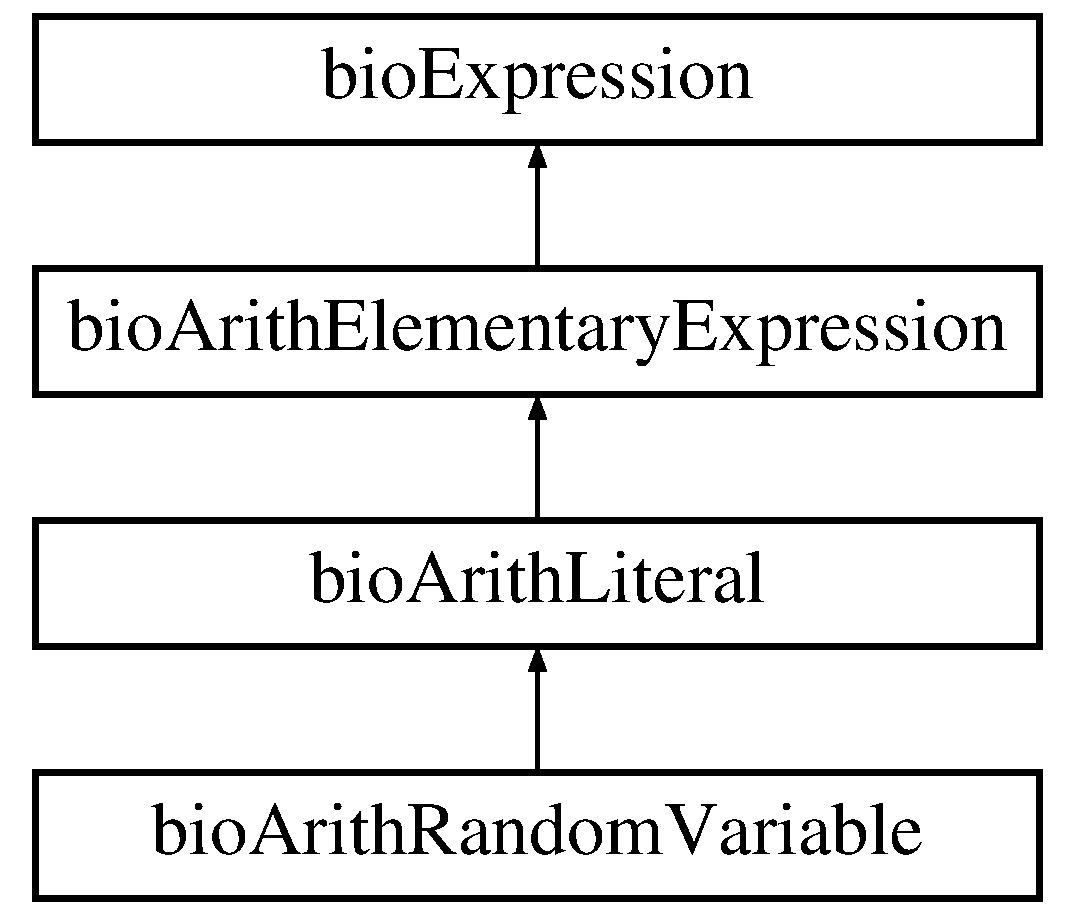
\includegraphics[height=4.000000cm]{classbio_arith_random_variable}
\end{center}
\end{figure}
\subsection*{Public Member Functions}
\begin{DoxyCompactItemize}
\item 
\mbox{\Hypertarget{classbio_arith_random_variable_a2ae1c241087441b487da80770d119257}\label{classbio_arith_random_variable_a2ae1c241087441b487da80770d119257}} 
{\bfseries bio\+Arith\+Random\+Variable} (\hyperlink{classbio_expression_repository}{bio\+Expression\+Repository} $\ast$rep, pat\+U\+Long par, pat\+U\+Long unique\+Id, pat\+U\+Long rv\+Id)
\item 
virtual \hyperlink{classbio_arith_random_variable}{bio\+Arith\+Random\+Variable} $\ast$ \hyperlink{classbio_arith_random_variable_a258a34932273d07449117a20704e7811}{get\+Deep\+Copy} (\hyperlink{classbio_expression_repository}{bio\+Expression\+Repository} $\ast$rep, pat\+Error $\ast$\&err) const
\item 
virtual \hyperlink{classbio_arith_random_variable}{bio\+Arith\+Random\+Variable} $\ast$ \hyperlink{classbio_arith_random_variable_a970e51cefe17a32b0c752e8bef35285f}{get\+Shallow\+Copy} (\hyperlink{classbio_expression_repository}{bio\+Expression\+Repository} $\ast$rep, pat\+Error $\ast$\&err) const
\item 
virtual pat\+Real \hyperlink{classbio_arith_random_variable_adc6a79d35ee6e66e59c3be9bc9f2c32b}{get\+Value} (pat\+Boolean prepare\+Gradient, pat\+U\+Long current\+Lap, pat\+Error $\ast$\&err)
\end{DoxyCompactItemize}
\subsection*{Protected Attributes}
\begin{DoxyCompactItemize}
\item 
\mbox{\Hypertarget{classbio_arith_random_variable_a587f811b4b070593f1983f4a475c91a1}\label{classbio_arith_random_variable_a587f811b4b070593f1983f4a475c91a1}} 
pat\+U\+Long {\bfseries the\+Random\+Variable\+Id}
\end{DoxyCompactItemize}


\subsection{Detailed Description}
Class implementing the node for a random variable used in an integral 

\subsection{Member Function Documentation}
\mbox{\Hypertarget{classbio_arith_random_variable_a258a34932273d07449117a20704e7811}\label{classbio_arith_random_variable_a258a34932273d07449117a20704e7811}} 
\index{bio\+Arith\+Random\+Variable@{bio\+Arith\+Random\+Variable}!get\+Deep\+Copy@{get\+Deep\+Copy}}
\index{get\+Deep\+Copy@{get\+Deep\+Copy}!bio\+Arith\+Random\+Variable@{bio\+Arith\+Random\+Variable}}
\subsubsection{\texorpdfstring{get\+Deep\+Copy()}{getDeepCopy()}}
{\footnotesize\ttfamily \hyperlink{classbio_arith_random_variable}{bio\+Arith\+Random\+Variable} $\ast$ bio\+Arith\+Random\+Variable\+::get\+Deep\+Copy (\begin{DoxyParamCaption}\item[{\hyperlink{classbio_expression_repository}{bio\+Expression\+Repository} $\ast$}]{rep,  }\item[{pat\+Error $\ast$\&}]{err }\end{DoxyParamCaption}) const\hspace{0.3cm}{\ttfamily [virtual]}}

Create a deep copy of the expression and returns a pointer to it. It means that new instances of the children are created. 

Reimplemented from \hyperlink{classbio_expression_a4ee1b8add634078a02eaae26cd40dcc8}{bio\+Expression}.

\mbox{\Hypertarget{classbio_arith_random_variable_a970e51cefe17a32b0c752e8bef35285f}\label{classbio_arith_random_variable_a970e51cefe17a32b0c752e8bef35285f}} 
\index{bio\+Arith\+Random\+Variable@{bio\+Arith\+Random\+Variable}!get\+Shallow\+Copy@{get\+Shallow\+Copy}}
\index{get\+Shallow\+Copy@{get\+Shallow\+Copy}!bio\+Arith\+Random\+Variable@{bio\+Arith\+Random\+Variable}}
\subsubsection{\texorpdfstring{get\+Shallow\+Copy()}{getShallowCopy()}}
{\footnotesize\ttfamily \hyperlink{classbio_arith_random_variable}{bio\+Arith\+Random\+Variable} $\ast$ bio\+Arith\+Random\+Variable\+::get\+Shallow\+Copy (\begin{DoxyParamCaption}\item[{\hyperlink{classbio_expression_repository}{bio\+Expression\+Repository} $\ast$}]{rep,  }\item[{pat\+Error $\ast$\&}]{err }\end{DoxyParamCaption}) const\hspace{0.3cm}{\ttfamily [virtual]}}

Create a shallow copy of the expression and returns a pointer to it. It means that no new instance of the children are created. It is typically called by the repository 

Reimplemented from \hyperlink{classbio_expression_a442534762693b92baaf33928979a1bf8}{bio\+Expression}.

\mbox{\Hypertarget{classbio_arith_random_variable_adc6a79d35ee6e66e59c3be9bc9f2c32b}\label{classbio_arith_random_variable_adc6a79d35ee6e66e59c3be9bc9f2c32b}} 
\index{bio\+Arith\+Random\+Variable@{bio\+Arith\+Random\+Variable}!get\+Value@{get\+Value}}
\index{get\+Value@{get\+Value}!bio\+Arith\+Random\+Variable@{bio\+Arith\+Random\+Variable}}
\subsubsection{\texorpdfstring{get\+Value()}{getValue()}}
{\footnotesize\ttfamily pat\+Real bio\+Arith\+Random\+Variable\+::get\+Value (\begin{DoxyParamCaption}\item[{pat\+Boolean}]{prepare\+Gradient,  }\item[{pat\+U\+Long}]{current\+Lap,  }\item[{pat\+Error $\ast$\&}]{err }\end{DoxyParamCaption})\hspace{0.3cm}{\ttfamily [virtual]}}

\begin{DoxyReturn}{Returns}
value of the expression 
\end{DoxyReturn}

\begin{DoxyParams}{Parameters}
{\em err} & ref. of the pointer to the error object. \\
\hline
\end{DoxyParams}


Reimplemented from \hyperlink{classbio_expression_af58662a5d4d456f15bc4f2c9bd4f8a5b}{bio\+Expression}.



The documentation for this class was generated from the following files\+:\begin{DoxyCompactItemize}
\item 
bio\+Arith\+Random\+Variable.\+h\item 
bio\+Arith\+Random\+Variable.\+cc\end{DoxyCompactItemize}

\hypertarget{classbio_arith_sum}{}\section{bio\+Arith\+Sum Class Reference}
\label{classbio_arith_sum}\index{bio\+Arith\+Sum@{bio\+Arith\+Sum}}


{\ttfamily \#include $<$bio\+Arith\+Sum.\+h$>$}

Inheritance diagram for bio\+Arith\+Sum\+:\begin{figure}[H]
\begin{center}
\leavevmode
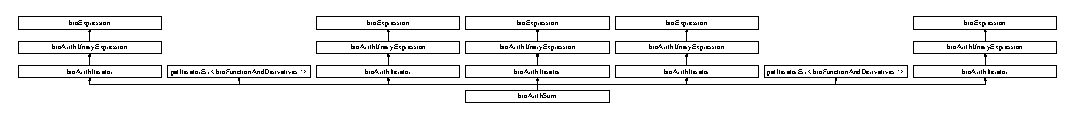
\includegraphics[height=1.146953cm]{classbio_arith_sum}
\end{center}
\end{figure}
\subsection*{Public Member Functions}
\begin{DoxyCompactItemize}
\item 
\mbox{\Hypertarget{classbio_arith_sum_af5f0818c44873b2cb1c10769468dca23}\label{classbio_arith_sum_af5f0818c44873b2cb1c10769468dca23}} 
{\bfseries bio\+Arith\+Sum} (\hyperlink{classbio_expression_repository}{bio\+Expression\+Repository} $\ast$rep, pat\+U\+Long par, pat\+U\+Long left, pat\+String an\+Iterator, pat\+U\+Long w, pat\+Error $\ast$\&err)
\item 
virtual \hyperlink{classbio_expression}{bio\+Expression} $\ast$ \hyperlink{classbio_arith_sum_acefb2c0e91cdea5768b09aa17974c25e}{get\+Derivative} (pat\+U\+Long a\+Literal\+Id, pat\+Error $\ast$\&err) const
\item 
\mbox{\Hypertarget{classbio_arith_sum_ae93d63173a732831f2eabb7bf3aca8e6}\label{classbio_arith_sum_ae93d63173a732831f2eabb7bf3aca8e6}} 
virtual tr\+Hessian $\ast$ {\bfseries get\+Bhhh} ()
\item 
virtual pat\+Boolean \hyperlink{classbio_arith_sum_a57d25760240c2d93b414d79679cfa5a3}{is\+Sum\+Iterator} () const
\item 
\mbox{\Hypertarget{classbio_arith_sum_a51e245ae7bcf17979c1207eefef8fc89}\label{classbio_arith_sum_a51e245ae7bcf17979c1207eefef8fc89}} 
virtual pat\+Boolean {\bfseries is\+Sum} () const
\item 
\mbox{\Hypertarget{classbio_arith_sum_a988363e77af268da7f58101b662b644b}\label{classbio_arith_sum_a988363e77af268da7f58101b662b644b}} 
virtual pat\+Boolean {\bfseries is\+Prod} () const
\item 
virtual pat\+String \hyperlink{classbio_arith_sum_a3bebc8a594c98febfad645befc1e6afa}{get\+Operator\+Name} () const
\item 
virtual \hyperlink{classbio_arith_sum}{bio\+Arith\+Sum} $\ast$ \hyperlink{classbio_arith_sum_ad32aa07569ab7c8f118a632f331e55d7}{get\+Deep\+Copy} (\hyperlink{classbio_expression_repository}{bio\+Expression\+Repository} $\ast$rep, pat\+Error $\ast$\&err) const
\item 
virtual \hyperlink{classbio_arith_sum}{bio\+Arith\+Sum} $\ast$ \hyperlink{classbio_arith_sum_ac2180e097ac045f893a789dd627b259a}{get\+Shallow\+Copy} (\hyperlink{classbio_expression_repository}{bio\+Expression\+Repository} $\ast$rep, pat\+Error $\ast$\&err) const
\item 
virtual pat\+String \hyperlink{classbio_arith_sum_ade9e163192f4124f802daf463d27faa4}{get\+Expression\+String} () const
\item 
virtual pat\+Real \hyperlink{classbio_arith_sum_a96362470d300fec04262c86df3864190}{get\+Value} (pat\+Boolean prepare\+Gradient, pat\+U\+Long current\+Lap, pat\+Error $\ast$\&err)
\item 
\mbox{\Hypertarget{classbio_arith_sum_a9793d7e0e30ec84780582eb7157c1f3e}\label{classbio_arith_sum_a9793d7e0e30ec84780582eb7157c1f3e}} 
virtual pat\+U\+Long {\bfseries get\+Number\+Of\+Operations} () const
\item 
virtual \hyperlink{classbio_function_and_derivatives}{bio\+Function\+And\+Derivatives} $\ast$ \hyperlink{classbio_arith_sum_a18cf2d6545bce0712f755c6eaf69407a}{get\+Numerical\+Function\+And\+Gradient} (vector$<$ pat\+U\+Long $>$ literal\+Ids, pat\+Boolean compute\+Hessian, pat\+Boolean debug\+Derivatives, pat\+Error $\ast$\&err)
\item 
\mbox{\Hypertarget{classbio_arith_sum_af5f0818c44873b2cb1c10769468dca23}\label{classbio_arith_sum_af5f0818c44873b2cb1c10769468dca23}} 
{\bfseries bio\+Arith\+Sum} (\hyperlink{classbio_expression_repository}{bio\+Expression\+Repository} $\ast$rep, pat\+U\+Long par, pat\+U\+Long left, pat\+String an\+Iterator, pat\+U\+Long w, pat\+Error $\ast$\&err)
\item 
virtual \hyperlink{classbio_expression}{bio\+Expression} $\ast$ \hyperlink{classbio_arith_sum_a2c030d0fea64581fe6f33031d3d3c977}{get\+Derivative} (pat\+U\+Long a\+Literal\+Id, pat\+Error $\ast$\&err) const
\item 
\mbox{\Hypertarget{classbio_arith_sum_ae22ebe2bc507588c53bdac6144381adf}\label{classbio_arith_sum_ae22ebe2bc507588c53bdac6144381adf}} 
virtual tr\+Hessian $\ast$ {\bfseries get\+Bhhh} ()
\item 
virtual pat\+Boolean \hyperlink{classbio_arith_sum_ab0747dc4d0f4fbe2cb246b265ec3cd11}{is\+Sum\+Iterator} () const
\item 
\mbox{\Hypertarget{classbio_arith_sum_ac2adee4ec319273e2e571a5dc3fd5fdf}\label{classbio_arith_sum_ac2adee4ec319273e2e571a5dc3fd5fdf}} 
virtual pat\+Boolean {\bfseries is\+Sum} () const
\item 
\mbox{\Hypertarget{classbio_arith_sum_a44affda18b23bdbfae680143df4293cb}\label{classbio_arith_sum_a44affda18b23bdbfae680143df4293cb}} 
virtual pat\+Boolean {\bfseries is\+Prod} () const
\item 
virtual pat\+String \hyperlink{classbio_arith_sum_a9e0ab0b9062a7cd80e70fc16505bc282}{get\+Operator\+Name} () const
\item 
virtual \hyperlink{classbio_arith_sum}{bio\+Arith\+Sum} $\ast$ \hyperlink{classbio_arith_sum_ab3264f5810c52c59b96ae72370e441ff}{get\+Deep\+Copy} (\hyperlink{classbio_expression_repository}{bio\+Expression\+Repository} $\ast$rep, pat\+Error $\ast$\&err) const
\item 
virtual \hyperlink{classbio_arith_sum}{bio\+Arith\+Sum} $\ast$ \hyperlink{classbio_arith_sum_a0828ed33f49201118b143dfa336d9212}{get\+Shallow\+Copy} (\hyperlink{classbio_expression_repository}{bio\+Expression\+Repository} $\ast$rep, pat\+Error $\ast$\&err) const
\item 
virtual pat\+String \hyperlink{classbio_arith_sum_a1354d70bccf4ba5e3d8ca634005d5489}{get\+Expression\+String} () const
\item 
virtual pat\+Real \hyperlink{classbio_arith_sum_a3705cb2f1aebf4541131df5638a33379}{get\+Value} (pat\+Boolean prepare\+Gradient, pat\+U\+Long current\+Lap, pat\+Error $\ast$\&err)
\item 
\mbox{\Hypertarget{classbio_arith_sum_ab192ab3a089be64024a110d94a341fb3}\label{classbio_arith_sum_ab192ab3a089be64024a110d94a341fb3}} 
virtual pat\+U\+Long {\bfseries get\+Number\+Of\+Operations} () const
\item 
virtual \hyperlink{classbio_function_and_derivatives}{bio\+Function\+And\+Derivatives} $\ast$ \hyperlink{classbio_arith_sum_afe9b54bab626e9dbe2b3aefebbcb6f8f}{get\+Numerical\+Function\+And\+Gradient} (vector$<$ pat\+U\+Long $>$ literal\+Ids, pat\+Boolean compute\+Hessian, pat\+Boolean debug\+Derivatives, pat\+Error $\ast$\&err)
\item 
\mbox{\Hypertarget{classbio_arith_sum_a40f9c410ecce415e6f542f08d6e5cf18}\label{classbio_arith_sum_a40f9c410ecce415e6f542f08d6e5cf18}} 
pat\+Iterator\+Err$<$ \hyperlink{classbio_function_and_derivatives}{bio\+Function\+And\+Derivatives} $\ast$ $>$ $\ast$ {\bfseries get\+Iterator\+For\+Stochastic\+Gradient} (pat\+Error $\ast$\&err)
\item 
\mbox{\Hypertarget{classbio_arith_sum_aba70598e4a7de1d36d34c6bb693a3ebf}\label{classbio_arith_sum_aba70598e4a7de1d36d34c6bb693a3ebf}} 
void {\bfseries first} (pat\+Error $\ast$\&err)
\item 
\mbox{\Hypertarget{classbio_arith_sum_a8f37c0eccb1fdc7f6aea57053332e438}\label{classbio_arith_sum_a8f37c0eccb1fdc7f6aea57053332e438}} 
void {\bfseries next} (pat\+Error $\ast$\&err)
\item 
\mbox{\Hypertarget{classbio_arith_sum_a22b293eefd5b26bdc102d2dbe938e5fd}\label{classbio_arith_sum_a22b293eefd5b26bdc102d2dbe938e5fd}} 
pat\+Boolean {\bfseries is\+Done} (pat\+Error $\ast$\&err)
\item 
\mbox{\Hypertarget{classbio_arith_sum_adef00302e992d944a9cd48c6e4050996}\label{classbio_arith_sum_adef00302e992d944a9cd48c6e4050996}} 
\hyperlink{classbio_function_and_derivatives}{bio\+Function\+And\+Derivatives} $\ast$ {\bfseries current\+Item} (pat\+Error $\ast$\&err)
\item 
\mbox{\Hypertarget{classbio_arith_sum_a6afd62a5e7a17d2f4b8268b07aee7ba8}\label{classbio_arith_sum_a6afd62a5e7a17d2f4b8268b07aee7ba8}} 
{\bfseries bio\+Arith\+Sum} (\hyperlink{classbio_expression}{bio\+Expression} $\ast$par, \hyperlink{classbio_expression}{bio\+Expression} $\ast$left, \hyperlink{classbio_iterator_info}{bio\+Iterator\+Info} $\ast$an\+Iterator)
\item 
\mbox{\Hypertarget{classbio_arith_sum_a58684f56172a3200a4caaeaad00b070d}\label{classbio_arith_sum_a58684f56172a3200a4caaeaad00b070d}} 
virtual {\bfseries is\+Sum} () const
\item 
\mbox{\Hypertarget{classbio_arith_sum_a9e85e0def0ec3e7eeba4a93ef508337e}\label{classbio_arith_sum_a9e85e0def0ec3e7eeba4a93ef508337e}} 
virtual {\bfseries is\+Prod} () const
\item 
\mbox{\Hypertarget{classbio_arith_sum_af5f0818c44873b2cb1c10769468dca23}\label{classbio_arith_sum_af5f0818c44873b2cb1c10769468dca23}} 
{\bfseries bio\+Arith\+Sum} (\hyperlink{classbio_expression_repository}{bio\+Expression\+Repository} $\ast$rep, pat\+U\+Long par, pat\+U\+Long left, pat\+String an\+Iterator, pat\+U\+Long w, pat\+Error $\ast$\&err)
\item 
virtual \hyperlink{classbio_expression}{bio\+Expression} $\ast$ \hyperlink{classbio_arith_sum_a2c030d0fea64581fe6f33031d3d3c977}{get\+Derivative} (pat\+U\+Long a\+Literal\+Id, pat\+Error $\ast$\&err) const
\item 
\mbox{\Hypertarget{classbio_arith_sum_ae22ebe2bc507588c53bdac6144381adf}\label{classbio_arith_sum_ae22ebe2bc507588c53bdac6144381adf}} 
virtual tr\+Hessian $\ast$ {\bfseries get\+Bhhh} ()
\item 
virtual pat\+Boolean \hyperlink{classbio_arith_sum_ab0747dc4d0f4fbe2cb246b265ec3cd11}{is\+Sum\+Iterator} () const
\item 
\mbox{\Hypertarget{classbio_arith_sum_ac2adee4ec319273e2e571a5dc3fd5fdf}\label{classbio_arith_sum_ac2adee4ec319273e2e571a5dc3fd5fdf}} 
virtual pat\+Boolean {\bfseries is\+Sum} () const
\item 
\mbox{\Hypertarget{classbio_arith_sum_a44affda18b23bdbfae680143df4293cb}\label{classbio_arith_sum_a44affda18b23bdbfae680143df4293cb}} 
virtual pat\+Boolean {\bfseries is\+Prod} () const
\item 
virtual pat\+String \hyperlink{classbio_arith_sum_a9e0ab0b9062a7cd80e70fc16505bc282}{get\+Operator\+Name} () const
\item 
virtual \hyperlink{classbio_arith_sum}{bio\+Arith\+Sum} $\ast$ \hyperlink{classbio_arith_sum_ab3264f5810c52c59b96ae72370e441ff}{get\+Deep\+Copy} (\hyperlink{classbio_expression_repository}{bio\+Expression\+Repository} $\ast$rep, pat\+Error $\ast$\&err) const
\item 
virtual \hyperlink{classbio_arith_sum}{bio\+Arith\+Sum} $\ast$ \hyperlink{classbio_arith_sum_a0828ed33f49201118b143dfa336d9212}{get\+Shallow\+Copy} (\hyperlink{classbio_expression_repository}{bio\+Expression\+Repository} $\ast$rep, pat\+Error $\ast$\&err) const
\item 
virtual pat\+String \hyperlink{classbio_arith_sum_a1354d70bccf4ba5e3d8ca634005d5489}{get\+Expression\+String} () const
\item 
virtual pat\+Real \hyperlink{classbio_arith_sum_a3705cb2f1aebf4541131df5638a33379}{get\+Value} (pat\+Boolean prepare\+Gradient, pat\+U\+Long current\+Lap, pat\+Error $\ast$\&err)
\item 
\mbox{\Hypertarget{classbio_arith_sum_ab192ab3a089be64024a110d94a341fb3}\label{classbio_arith_sum_ab192ab3a089be64024a110d94a341fb3}} 
virtual pat\+U\+Long {\bfseries get\+Number\+Of\+Operations} () const
\item 
virtual \hyperlink{classbio_function_and_derivatives}{bio\+Function\+And\+Derivatives} $\ast$ \hyperlink{classbio_arith_sum_afe9b54bab626e9dbe2b3aefebbcb6f8f}{get\+Numerical\+Function\+And\+Gradient} (vector$<$ pat\+U\+Long $>$ literal\+Ids, pat\+Boolean compute\+Hessian, pat\+Boolean debug\+Derivatives, pat\+Error $\ast$\&err)
\item 
\mbox{\Hypertarget{classbio_arith_sum_af5f0818c44873b2cb1c10769468dca23}\label{classbio_arith_sum_af5f0818c44873b2cb1c10769468dca23}} 
{\bfseries bio\+Arith\+Sum} (\hyperlink{classbio_expression_repository}{bio\+Expression\+Repository} $\ast$rep, pat\+U\+Long par, pat\+U\+Long left, pat\+String an\+Iterator, pat\+U\+Long w, pat\+Error $\ast$\&err)
\item 
virtual \hyperlink{classbio_expression}{bio\+Expression} $\ast$ \hyperlink{classbio_arith_sum_a2c030d0fea64581fe6f33031d3d3c977}{get\+Derivative} (pat\+U\+Long a\+Literal\+Id, pat\+Error $\ast$\&err) const
\item 
\mbox{\Hypertarget{classbio_arith_sum_ae22ebe2bc507588c53bdac6144381adf}\label{classbio_arith_sum_ae22ebe2bc507588c53bdac6144381adf}} 
virtual tr\+Hessian $\ast$ {\bfseries get\+Bhhh} ()
\item 
virtual pat\+Boolean \hyperlink{classbio_arith_sum_ab0747dc4d0f4fbe2cb246b265ec3cd11}{is\+Sum\+Iterator} () const
\item 
\mbox{\Hypertarget{classbio_arith_sum_ac2adee4ec319273e2e571a5dc3fd5fdf}\label{classbio_arith_sum_ac2adee4ec319273e2e571a5dc3fd5fdf}} 
virtual pat\+Boolean {\bfseries is\+Sum} () const
\item 
\mbox{\Hypertarget{classbio_arith_sum_a44affda18b23bdbfae680143df4293cb}\label{classbio_arith_sum_a44affda18b23bdbfae680143df4293cb}} 
virtual pat\+Boolean {\bfseries is\+Prod} () const
\item 
virtual pat\+String \hyperlink{classbio_arith_sum_a9e0ab0b9062a7cd80e70fc16505bc282}{get\+Operator\+Name} () const
\item 
virtual \hyperlink{classbio_arith_sum}{bio\+Arith\+Sum} $\ast$ \hyperlink{classbio_arith_sum_ab3264f5810c52c59b96ae72370e441ff}{get\+Deep\+Copy} (\hyperlink{classbio_expression_repository}{bio\+Expression\+Repository} $\ast$rep, pat\+Error $\ast$\&err) const
\item 
virtual \hyperlink{classbio_arith_sum}{bio\+Arith\+Sum} $\ast$ \hyperlink{classbio_arith_sum_a0828ed33f49201118b143dfa336d9212}{get\+Shallow\+Copy} (\hyperlink{classbio_expression_repository}{bio\+Expression\+Repository} $\ast$rep, pat\+Error $\ast$\&err) const
\item 
virtual pat\+String \hyperlink{classbio_arith_sum_a1354d70bccf4ba5e3d8ca634005d5489}{get\+Expression\+String} () const
\item 
virtual pat\+Real \hyperlink{classbio_arith_sum_a3705cb2f1aebf4541131df5638a33379}{get\+Value} (pat\+Boolean prepare\+Gradient, pat\+U\+Long current\+Lap, pat\+Error $\ast$\&err)
\item 
\mbox{\Hypertarget{classbio_arith_sum_ab192ab3a089be64024a110d94a341fb3}\label{classbio_arith_sum_ab192ab3a089be64024a110d94a341fb3}} 
virtual pat\+U\+Long {\bfseries get\+Number\+Of\+Operations} () const
\item 
virtual \hyperlink{classbio_function_and_derivatives}{bio\+Function\+And\+Derivatives} $\ast$ \hyperlink{classbio_arith_sum_afe9b54bab626e9dbe2b3aefebbcb6f8f}{get\+Numerical\+Function\+And\+Gradient} (vector$<$ pat\+U\+Long $>$ literal\+Ids, pat\+Boolean compute\+Hessian, pat\+Boolean debug\+Derivatives, pat\+Error $\ast$\&err)
\item 
\mbox{\Hypertarget{classbio_arith_sum_a6defac5816d2b12e96482a97b2c08484}\label{classbio_arith_sum_a6defac5816d2b12e96482a97b2c08484}} 
pat\+Iterator$<$ \hyperlink{classbio_function_and_derivatives}{bio\+Function\+And\+Derivatives} $\ast$ $>$ $\ast$ {\bfseries get\+Iterator\+For\+Stochastic\+Gradient} ()
\item 
\mbox{\Hypertarget{classbio_arith_sum_aba70598e4a7de1d36d34c6bb693a3ebf}\label{classbio_arith_sum_aba70598e4a7de1d36d34c6bb693a3ebf}} 
void {\bfseries first} (pat\+Error $\ast$\&err)
\item 
\mbox{\Hypertarget{classbio_arith_sum_a8f37c0eccb1fdc7f6aea57053332e438}\label{classbio_arith_sum_a8f37c0eccb1fdc7f6aea57053332e438}} 
void {\bfseries next} (pat\+Error $\ast$\&err)
\item 
\mbox{\Hypertarget{classbio_arith_sum_a22b293eefd5b26bdc102d2dbe938e5fd}\label{classbio_arith_sum_a22b293eefd5b26bdc102d2dbe938e5fd}} 
pat\+Boolean {\bfseries is\+Done} (pat\+Error $\ast$\&err)
\item 
\mbox{\Hypertarget{classbio_arith_sum_ab572e72d4fe22ab773ba8e61d5c18c69}\label{classbio_arith_sum_ab572e72d4fe22ab773ba8e61d5c18c69}} 
\hyperlink{classbio_function_and_derivatives}{bio\+Function\+And\+Derivatives} $\ast$ {\bfseries current\+Item} (pat\+Error $\ast$\&err)
\end{DoxyCompactItemize}
\subsection*{Additional Inherited Members}


\subsection{Detailed Description}
Class implementing a node of the tree representing a sum expression 

\subsection{Member Function Documentation}
\mbox{\Hypertarget{classbio_arith_sum_ab3264f5810c52c59b96ae72370e441ff}\label{classbio_arith_sum_ab3264f5810c52c59b96ae72370e441ff}} 
\index{bio\+Arith\+Sum@{bio\+Arith\+Sum}!get\+Deep\+Copy@{get\+Deep\+Copy}}
\index{get\+Deep\+Copy@{get\+Deep\+Copy}!bio\+Arith\+Sum@{bio\+Arith\+Sum}}
\subsubsection{\texorpdfstring{get\+Deep\+Copy()}{getDeepCopy()}\hspace{0.1cm}{\footnotesize\ttfamily [1/4]}}
{\footnotesize\ttfamily virtual \hyperlink{classbio_arith_sum}{bio\+Arith\+Sum}$\ast$ bio\+Arith\+Sum\+::get\+Deep\+Copy (\begin{DoxyParamCaption}\item[{\hyperlink{classbio_expression_repository}{bio\+Expression\+Repository} $\ast$}]{rep,  }\item[{pat\+Error $\ast$\&}]{err }\end{DoxyParamCaption}) const\hspace{0.3cm}{\ttfamily [virtual]}}

Create a deep copy of the expression and returns a pointer to it. It means that new instances of the children are created. 

Reimplemented from \hyperlink{classbio_expression_a4ee1b8add634078a02eaae26cd40dcc8}{bio\+Expression}.

\mbox{\Hypertarget{classbio_arith_sum_ad32aa07569ab7c8f118a632f331e55d7}\label{classbio_arith_sum_ad32aa07569ab7c8f118a632f331e55d7}} 
\index{bio\+Arith\+Sum@{bio\+Arith\+Sum}!get\+Deep\+Copy@{get\+Deep\+Copy}}
\index{get\+Deep\+Copy@{get\+Deep\+Copy}!bio\+Arith\+Sum@{bio\+Arith\+Sum}}
\subsubsection{\texorpdfstring{get\+Deep\+Copy()}{getDeepCopy()}\hspace{0.1cm}{\footnotesize\ttfamily [2/4]}}
{\footnotesize\ttfamily \hyperlink{classbio_arith_sum}{bio\+Arith\+Sum} $\ast$ bio\+Arith\+Sum\+::get\+Deep\+Copy (\begin{DoxyParamCaption}\item[{\hyperlink{classbio_expression_repository}{bio\+Expression\+Repository} $\ast$}]{rep,  }\item[{pat\+Error $\ast$\&}]{err }\end{DoxyParamCaption}) const\hspace{0.3cm}{\ttfamily [virtual]}}

Create a deep copy of the expression and returns a pointer to it. It means that new instances of the children are created. 

Reimplemented from \hyperlink{classbio_expression_a4ee1b8add634078a02eaae26cd40dcc8}{bio\+Expression}.

\mbox{\Hypertarget{classbio_arith_sum_ab3264f5810c52c59b96ae72370e441ff}\label{classbio_arith_sum_ab3264f5810c52c59b96ae72370e441ff}} 
\index{bio\+Arith\+Sum@{bio\+Arith\+Sum}!get\+Deep\+Copy@{get\+Deep\+Copy}}
\index{get\+Deep\+Copy@{get\+Deep\+Copy}!bio\+Arith\+Sum@{bio\+Arith\+Sum}}
\subsubsection{\texorpdfstring{get\+Deep\+Copy()}{getDeepCopy()}\hspace{0.1cm}{\footnotesize\ttfamily [3/4]}}
{\footnotesize\ttfamily virtual \hyperlink{classbio_arith_sum}{bio\+Arith\+Sum}$\ast$ bio\+Arith\+Sum\+::get\+Deep\+Copy (\begin{DoxyParamCaption}\item[{\hyperlink{classbio_expression_repository}{bio\+Expression\+Repository} $\ast$}]{rep,  }\item[{pat\+Error $\ast$\&}]{err }\end{DoxyParamCaption}) const\hspace{0.3cm}{\ttfamily [virtual]}}

Create a deep copy of the expression and returns a pointer to it. It means that new instances of the children are created. 

Reimplemented from \hyperlink{classbio_expression_a4ee1b8add634078a02eaae26cd40dcc8}{bio\+Expression}.

\mbox{\Hypertarget{classbio_arith_sum_ab3264f5810c52c59b96ae72370e441ff}\label{classbio_arith_sum_ab3264f5810c52c59b96ae72370e441ff}} 
\index{bio\+Arith\+Sum@{bio\+Arith\+Sum}!get\+Deep\+Copy@{get\+Deep\+Copy}}
\index{get\+Deep\+Copy@{get\+Deep\+Copy}!bio\+Arith\+Sum@{bio\+Arith\+Sum}}
\subsubsection{\texorpdfstring{get\+Deep\+Copy()}{getDeepCopy()}\hspace{0.1cm}{\footnotesize\ttfamily [4/4]}}
{\footnotesize\ttfamily virtual \hyperlink{classbio_arith_sum}{bio\+Arith\+Sum}$\ast$ bio\+Arith\+Sum\+::get\+Deep\+Copy (\begin{DoxyParamCaption}\item[{\hyperlink{classbio_expression_repository}{bio\+Expression\+Repository} $\ast$}]{rep,  }\item[{pat\+Error $\ast$\&}]{err }\end{DoxyParamCaption}) const\hspace{0.3cm}{\ttfamily [virtual]}}

Create a deep copy of the expression and returns a pointer to it. It means that new instances of the children are created. 

Reimplemented from \hyperlink{classbio_expression_a4ee1b8add634078a02eaae26cd40dcc8}{bio\+Expression}.

\mbox{\Hypertarget{classbio_arith_sum_acefb2c0e91cdea5768b09aa17974c25e}\label{classbio_arith_sum_acefb2c0e91cdea5768b09aa17974c25e}} 
\index{bio\+Arith\+Sum@{bio\+Arith\+Sum}!get\+Derivative@{get\+Derivative}}
\index{get\+Derivative@{get\+Derivative}!bio\+Arith\+Sum@{bio\+Arith\+Sum}}
\subsubsection{\texorpdfstring{get\+Derivative()}{getDerivative()}\hspace{0.1cm}{\footnotesize\ttfamily [1/4]}}
{\footnotesize\ttfamily \hyperlink{classbio_expression}{bio\+Expression} $\ast$ bio\+Arith\+Sum\+::get\+Derivative (\begin{DoxyParamCaption}\item[{pat\+U\+Long}]{a\+Literal\+Id,  }\item[{pat\+Error $\ast$\&}]{err }\end{DoxyParamCaption}) const\hspace{0.3cm}{\ttfamily [virtual]}}

\begin{DoxyReturn}{Returns}
value of the derivative w.\+r.\+t literal 
\end{DoxyReturn}

\begin{DoxyParams}{Parameters}
{\em index} & of the literal involved in the derivative \\
\hline
{\em err} & ref. of the pointer to the error object. \\
\hline
\end{DoxyParams}


Reimplemented from \hyperlink{classbio_expression_a5915579d1193f25f216c1e273c97f2ce}{bio\+Expression}.

\mbox{\Hypertarget{classbio_arith_sum_a2c030d0fea64581fe6f33031d3d3c977}\label{classbio_arith_sum_a2c030d0fea64581fe6f33031d3d3c977}} 
\index{bio\+Arith\+Sum@{bio\+Arith\+Sum}!get\+Derivative@{get\+Derivative}}
\index{get\+Derivative@{get\+Derivative}!bio\+Arith\+Sum@{bio\+Arith\+Sum}}
\subsubsection{\texorpdfstring{get\+Derivative()}{getDerivative()}\hspace{0.1cm}{\footnotesize\ttfamily [2/4]}}
{\footnotesize\ttfamily virtual \hyperlink{classbio_expression}{bio\+Expression}$\ast$ bio\+Arith\+Sum\+::get\+Derivative (\begin{DoxyParamCaption}\item[{pat\+U\+Long}]{a\+Literal\+Id,  }\item[{pat\+Error $\ast$\&}]{err }\end{DoxyParamCaption}) const\hspace{0.3cm}{\ttfamily [virtual]}}

\begin{DoxyReturn}{Returns}
value of the derivative w.\+r.\+t literal 
\end{DoxyReturn}

\begin{DoxyParams}{Parameters}
{\em index} & of the literal involved in the derivative \\
\hline
{\em err} & ref. of the pointer to the error object. \\
\hline
\end{DoxyParams}


Reimplemented from \hyperlink{classbio_expression_a5915579d1193f25f216c1e273c97f2ce}{bio\+Expression}.

\mbox{\Hypertarget{classbio_arith_sum_a2c030d0fea64581fe6f33031d3d3c977}\label{classbio_arith_sum_a2c030d0fea64581fe6f33031d3d3c977}} 
\index{bio\+Arith\+Sum@{bio\+Arith\+Sum}!get\+Derivative@{get\+Derivative}}
\index{get\+Derivative@{get\+Derivative}!bio\+Arith\+Sum@{bio\+Arith\+Sum}}
\subsubsection{\texorpdfstring{get\+Derivative()}{getDerivative()}\hspace{0.1cm}{\footnotesize\ttfamily [3/4]}}
{\footnotesize\ttfamily virtual \hyperlink{classbio_expression}{bio\+Expression}$\ast$ bio\+Arith\+Sum\+::get\+Derivative (\begin{DoxyParamCaption}\item[{pat\+U\+Long}]{a\+Literal\+Id,  }\item[{pat\+Error $\ast$\&}]{err }\end{DoxyParamCaption}) const\hspace{0.3cm}{\ttfamily [virtual]}}

\begin{DoxyReturn}{Returns}
value of the derivative w.\+r.\+t literal 
\end{DoxyReturn}

\begin{DoxyParams}{Parameters}
{\em index} & of the literal involved in the derivative \\
\hline
{\em err} & ref. of the pointer to the error object. \\
\hline
\end{DoxyParams}


Reimplemented from \hyperlink{classbio_expression_a5915579d1193f25f216c1e273c97f2ce}{bio\+Expression}.

\mbox{\Hypertarget{classbio_arith_sum_a2c030d0fea64581fe6f33031d3d3c977}\label{classbio_arith_sum_a2c030d0fea64581fe6f33031d3d3c977}} 
\index{bio\+Arith\+Sum@{bio\+Arith\+Sum}!get\+Derivative@{get\+Derivative}}
\index{get\+Derivative@{get\+Derivative}!bio\+Arith\+Sum@{bio\+Arith\+Sum}}
\subsubsection{\texorpdfstring{get\+Derivative()}{getDerivative()}\hspace{0.1cm}{\footnotesize\ttfamily [4/4]}}
{\footnotesize\ttfamily virtual \hyperlink{classbio_expression}{bio\+Expression}$\ast$ bio\+Arith\+Sum\+::get\+Derivative (\begin{DoxyParamCaption}\item[{pat\+U\+Long}]{a\+Literal\+Id,  }\item[{pat\+Error $\ast$\&}]{err }\end{DoxyParamCaption}) const\hspace{0.3cm}{\ttfamily [virtual]}}

\begin{DoxyReturn}{Returns}
value of the derivative w.\+r.\+t literal 
\end{DoxyReturn}

\begin{DoxyParams}{Parameters}
{\em index} & of the literal involved in the derivative \\
\hline
{\em err} & ref. of the pointer to the error object. \\
\hline
\end{DoxyParams}


Reimplemented from \hyperlink{classbio_expression_a5915579d1193f25f216c1e273c97f2ce}{bio\+Expression}.

\mbox{\Hypertarget{classbio_arith_sum_ade9e163192f4124f802daf463d27faa4}\label{classbio_arith_sum_ade9e163192f4124f802daf463d27faa4}} 
\index{bio\+Arith\+Sum@{bio\+Arith\+Sum}!get\+Expression\+String@{get\+Expression\+String}}
\index{get\+Expression\+String@{get\+Expression\+String}!bio\+Arith\+Sum@{bio\+Arith\+Sum}}
\subsubsection{\texorpdfstring{get\+Expression\+String()}{getExpressionString()}\hspace{0.1cm}{\footnotesize\ttfamily [1/4]}}
{\footnotesize\ttfamily pat\+String bio\+Arith\+Sum\+::get\+Expression\+String (\begin{DoxyParamCaption}{ }\end{DoxyParamCaption}) const\hspace{0.3cm}{\ttfamily [virtual]}}

Compute a string that represents the expression. It is designed to replace the expression itself when used only for comparison purposes. Code\+: +\{expr1\}\{expr2\}\+: binary plus -\/\{expr1\}\{expr2\}\+: binary minus \{expr1\}\{expr2\}\+: multiplication /\{expr1\}\{expr2\}\+: division $^\wedge$\{expr1\}\{expr2\}\+: power \&\{expr1\}\{expr2\}\+: and $\vert$\{expr1\}\{expr2\}\+: or =\{expr1\}\{expr2\}\+: equal !=\{expr1\}\{expr2\}\+: not equal $<$\{expr1\}\{expr2\}\+: lesser than $<$=\{expr1\}\{expr2\}\+: lesser or equal to $>$\{expr1\}\{expr2\}\+: greater than $>$=\{expr1\}\{expr2\}\+: greater or equal to \$A\{expr\}\+: abs \$D\mbox{[}expr\mbox{]}\mbox{[}\{expr1\}...\{exprN\}\mbox{]}\+: dictionary (\hyperlink{classbio_arith_elem}{bio\+Arith\+Elem}) \$E\{expr\}\+: exp \$L\{expr\}\+: log \$M\{expr\}\+: Unary minus \$\+Piterator\+\_\+name\{expr\}\+: prod \$Q\{string1\}\{string2\}\+: sequence \$\+Siterator\+\_\+name\{expr\}\+: sum \$\+Ziterator\+\_\+name\mbox{[}\{expr1\}...\{exprN\}\mbox{]}\+: merged sum \{expr1\}\{expr2\}...\{exprN\}//\+: list of expressions number\+: constant \#id\+: literal \&id\+: random 

Reimplemented from \hyperlink{classbio_expression_a3e4b4dca58dbbc6f0e411b30eb3f60b4}{bio\+Expression}.

\mbox{\Hypertarget{classbio_arith_sum_a1354d70bccf4ba5e3d8ca634005d5489}\label{classbio_arith_sum_a1354d70bccf4ba5e3d8ca634005d5489}} 
\index{bio\+Arith\+Sum@{bio\+Arith\+Sum}!get\+Expression\+String@{get\+Expression\+String}}
\index{get\+Expression\+String@{get\+Expression\+String}!bio\+Arith\+Sum@{bio\+Arith\+Sum}}
\subsubsection{\texorpdfstring{get\+Expression\+String()}{getExpressionString()}\hspace{0.1cm}{\footnotesize\ttfamily [2/4]}}
{\footnotesize\ttfamily virtual pat\+String bio\+Arith\+Sum\+::get\+Expression\+String (\begin{DoxyParamCaption}{ }\end{DoxyParamCaption}) const\hspace{0.3cm}{\ttfamily [virtual]}}

Compute a string that represents the expression. It is designed to replace the expression itself when used only for comparison purposes. Code\+: +\{expr1\}\{expr2\}\+: binary plus -\/\{expr1\}\{expr2\}\+: binary minus \{expr1\}\{expr2\}\+: multiplication /\{expr1\}\{expr2\}\+: division $^\wedge$\{expr1\}\{expr2\}\+: power \&\{expr1\}\{expr2\}\+: and $\vert$\{expr1\}\{expr2\}\+: or =\{expr1\}\{expr2\}\+: equal !=\{expr1\}\{expr2\}\+: not equal $<$\{expr1\}\{expr2\}\+: lesser than $<$=\{expr1\}\{expr2\}\+: lesser or equal to $>$\{expr1\}\{expr2\}\+: greater than $>$=\{expr1\}\{expr2\}\+: greater or equal to \$A\{expr\}\+: abs \$D\mbox{[}expr\mbox{]}\mbox{[}\{expr1\}...\{exprN\}\mbox{]}\+: dictionary (\hyperlink{classbio_arith_elem}{bio\+Arith\+Elem}) \$E\{expr\}\+: exp \$L\{expr\}\+: log \$M\{expr\}\+: Unary minus \$\+Piterator\+\_\+name\{expr\}\+: prod \$Q\{string1\}\{string2\}\+: sequence \$\+Siterator\+\_\+name\{expr\}\+: sum \$\+Ziterator\+\_\+name\mbox{[}\{expr1\}...\{exprN\}\mbox{]}\+: merged sum \{expr1\}\{expr2\}...\{exprN\}//\+: list of expressions number\+: constant \#id\+: literal \&id\+: random 

Reimplemented from \hyperlink{classbio_expression_a3e4b4dca58dbbc6f0e411b30eb3f60b4}{bio\+Expression}.

\mbox{\Hypertarget{classbio_arith_sum_a1354d70bccf4ba5e3d8ca634005d5489}\label{classbio_arith_sum_a1354d70bccf4ba5e3d8ca634005d5489}} 
\index{bio\+Arith\+Sum@{bio\+Arith\+Sum}!get\+Expression\+String@{get\+Expression\+String}}
\index{get\+Expression\+String@{get\+Expression\+String}!bio\+Arith\+Sum@{bio\+Arith\+Sum}}
\subsubsection{\texorpdfstring{get\+Expression\+String()}{getExpressionString()}\hspace{0.1cm}{\footnotesize\ttfamily [3/4]}}
{\footnotesize\ttfamily virtual pat\+String bio\+Arith\+Sum\+::get\+Expression\+String (\begin{DoxyParamCaption}{ }\end{DoxyParamCaption}) const\hspace{0.3cm}{\ttfamily [virtual]}}

Compute a string that represents the expression. It is designed to replace the expression itself when used only for comparison purposes. Code\+: +\{expr1\}\{expr2\}\+: binary plus -\/\{expr1\}\{expr2\}\+: binary minus \{expr1\}\{expr2\}\+: multiplication /\{expr1\}\{expr2\}\+: division $^\wedge$\{expr1\}\{expr2\}\+: power \&\{expr1\}\{expr2\}\+: and $\vert$\{expr1\}\{expr2\}\+: or =\{expr1\}\{expr2\}\+: equal !=\{expr1\}\{expr2\}\+: not equal $<$\{expr1\}\{expr2\}\+: lesser than $<$=\{expr1\}\{expr2\}\+: lesser or equal to $>$\{expr1\}\{expr2\}\+: greater than $>$=\{expr1\}\{expr2\}\+: greater or equal to \$A\{expr\}\+: abs \$D\mbox{[}expr\mbox{]}\mbox{[}\{expr1\}...\{exprN\}\mbox{]}\+: dictionary (\hyperlink{classbio_arith_elem}{bio\+Arith\+Elem}) \$E\{expr\}\+: exp \$L\{expr\}\+: log \$M\{expr\}\+: Unary minus \$\+Piterator\+\_\+name\{expr\}\+: prod \$Q\{string1\}\{string2\}\+: sequence \$\+Siterator\+\_\+name\{expr\}\+: sum \$\+Ziterator\+\_\+name\mbox{[}\{expr1\}...\{exprN\}\mbox{]}\+: merged sum \{expr1\}\{expr2\}...\{exprN\}//\+: list of expressions number\+: constant \#id\+: literal \&id\+: random 

Reimplemented from \hyperlink{classbio_expression_a3e4b4dca58dbbc6f0e411b30eb3f60b4}{bio\+Expression}.

\mbox{\Hypertarget{classbio_arith_sum_a1354d70bccf4ba5e3d8ca634005d5489}\label{classbio_arith_sum_a1354d70bccf4ba5e3d8ca634005d5489}} 
\index{bio\+Arith\+Sum@{bio\+Arith\+Sum}!get\+Expression\+String@{get\+Expression\+String}}
\index{get\+Expression\+String@{get\+Expression\+String}!bio\+Arith\+Sum@{bio\+Arith\+Sum}}
\subsubsection{\texorpdfstring{get\+Expression\+String()}{getExpressionString()}\hspace{0.1cm}{\footnotesize\ttfamily [4/4]}}
{\footnotesize\ttfamily virtual pat\+String bio\+Arith\+Sum\+::get\+Expression\+String (\begin{DoxyParamCaption}{ }\end{DoxyParamCaption}) const\hspace{0.3cm}{\ttfamily [virtual]}}

Compute a string that represents the expression. It is designed to replace the expression itself when used only for comparison purposes. Code\+: +\{expr1\}\{expr2\}\+: binary plus -\/\{expr1\}\{expr2\}\+: binary minus \{expr1\}\{expr2\}\+: multiplication /\{expr1\}\{expr2\}\+: division $^\wedge$\{expr1\}\{expr2\}\+: power \&\{expr1\}\{expr2\}\+: and $\vert$\{expr1\}\{expr2\}\+: or =\{expr1\}\{expr2\}\+: equal !=\{expr1\}\{expr2\}\+: not equal $<$\{expr1\}\{expr2\}\+: lesser than $<$=\{expr1\}\{expr2\}\+: lesser or equal to $>$\{expr1\}\{expr2\}\+: greater than $>$=\{expr1\}\{expr2\}\+: greater or equal to \$A\{expr\}\+: abs \$D\mbox{[}expr\mbox{]}\mbox{[}\{expr1\}...\{exprN\}\mbox{]}\+: dictionary (\hyperlink{classbio_arith_elem}{bio\+Arith\+Elem}) \$E\{expr\}\+: exp \$L\{expr\}\+: log \$M\{expr\}\+: Unary minus \$\+Piterator\+\_\+name\{expr\}\+: prod \$Q\{string1\}\{string2\}\+: sequence \$\+Siterator\+\_\+name\{expr\}\+: sum \$\+Ziterator\+\_\+name\mbox{[}\{expr1\}...\{exprN\}\mbox{]}\+: merged sum \{expr1\}\{expr2\}...\{exprN\}//\+: list of expressions number\+: constant \#id\+: literal \&id\+: random 

Reimplemented from \hyperlink{classbio_expression_a3e4b4dca58dbbc6f0e411b30eb3f60b4}{bio\+Expression}.

\mbox{\Hypertarget{classbio_arith_sum_afe9b54bab626e9dbe2b3aefebbcb6f8f}\label{classbio_arith_sum_afe9b54bab626e9dbe2b3aefebbcb6f8f}} 
\index{bio\+Arith\+Sum@{bio\+Arith\+Sum}!get\+Numerical\+Function\+And\+Gradient@{get\+Numerical\+Function\+And\+Gradient}}
\index{get\+Numerical\+Function\+And\+Gradient@{get\+Numerical\+Function\+And\+Gradient}!bio\+Arith\+Sum@{bio\+Arith\+Sum}}
\subsubsection{\texorpdfstring{get\+Numerical\+Function\+And\+Gradient()}{getNumericalFunctionAndGradient()}\hspace{0.1cm}{\footnotesize\ttfamily [1/4]}}
{\footnotesize\ttfamily virtual \hyperlink{classbio_function_and_derivatives}{bio\+Function\+And\+Derivatives}$\ast$ bio\+Arith\+Sum\+::get\+Numerical\+Function\+And\+Gradient (\begin{DoxyParamCaption}\item[{vector$<$ pat\+U\+Long $>$}]{literal\+Ids,  }\item[{pat\+Boolean}]{compute\+Hessian,  }\item[{pat\+Boolean}]{debug\+Derivatives,  }\item[{pat\+Error $\ast$\&}]{err }\end{DoxyParamCaption})\hspace{0.3cm}{\ttfamily [virtual]}}

\begin{DoxyReturn}{Returns}
value and gradient of the expression 
\end{DoxyReturn}

\begin{DoxyParams}{Parameters}
{\em err} & ref. of the pointer to the error object. \\
\hline
\end{DoxyParams}


Reimplemented from \hyperlink{classbio_expression_a91c81ce80c9e972c913b10f5f3c1ed13}{bio\+Expression}.

\mbox{\Hypertarget{classbio_arith_sum_a18cf2d6545bce0712f755c6eaf69407a}\label{classbio_arith_sum_a18cf2d6545bce0712f755c6eaf69407a}} 
\index{bio\+Arith\+Sum@{bio\+Arith\+Sum}!get\+Numerical\+Function\+And\+Gradient@{get\+Numerical\+Function\+And\+Gradient}}
\index{get\+Numerical\+Function\+And\+Gradient@{get\+Numerical\+Function\+And\+Gradient}!bio\+Arith\+Sum@{bio\+Arith\+Sum}}
\subsubsection{\texorpdfstring{get\+Numerical\+Function\+And\+Gradient()}{getNumericalFunctionAndGradient()}\hspace{0.1cm}{\footnotesize\ttfamily [2/4]}}
{\footnotesize\ttfamily \hyperlink{classbio_function_and_derivatives}{bio\+Function\+And\+Derivatives} $\ast$ bio\+Arith\+Sum\+::get\+Numerical\+Function\+And\+Gradient (\begin{DoxyParamCaption}\item[{vector$<$ pat\+U\+Long $>$}]{literal\+Ids,  }\item[{pat\+Boolean}]{compute\+Hessian,  }\item[{pat\+Boolean}]{debug\+Derivatives,  }\item[{pat\+Error $\ast$\&}]{err }\end{DoxyParamCaption})\hspace{0.3cm}{\ttfamily [virtual]}}

\begin{DoxyReturn}{Returns}
value and gradient of the expression 
\end{DoxyReturn}

\begin{DoxyParams}{Parameters}
{\em err} & ref. of the pointer to the error object. \\
\hline
\end{DoxyParams}


Reimplemented from \hyperlink{classbio_expression_a91c81ce80c9e972c913b10f5f3c1ed13}{bio\+Expression}.

\mbox{\Hypertarget{classbio_arith_sum_afe9b54bab626e9dbe2b3aefebbcb6f8f}\label{classbio_arith_sum_afe9b54bab626e9dbe2b3aefebbcb6f8f}} 
\index{bio\+Arith\+Sum@{bio\+Arith\+Sum}!get\+Numerical\+Function\+And\+Gradient@{get\+Numerical\+Function\+And\+Gradient}}
\index{get\+Numerical\+Function\+And\+Gradient@{get\+Numerical\+Function\+And\+Gradient}!bio\+Arith\+Sum@{bio\+Arith\+Sum}}
\subsubsection{\texorpdfstring{get\+Numerical\+Function\+And\+Gradient()}{getNumericalFunctionAndGradient()}\hspace{0.1cm}{\footnotesize\ttfamily [3/4]}}
{\footnotesize\ttfamily virtual \hyperlink{classbio_function_and_derivatives}{bio\+Function\+And\+Derivatives}$\ast$ bio\+Arith\+Sum\+::get\+Numerical\+Function\+And\+Gradient (\begin{DoxyParamCaption}\item[{vector$<$ pat\+U\+Long $>$}]{literal\+Ids,  }\item[{pat\+Boolean}]{compute\+Hessian,  }\item[{pat\+Boolean}]{debug\+Derivatives,  }\item[{pat\+Error $\ast$\&}]{err }\end{DoxyParamCaption})\hspace{0.3cm}{\ttfamily [virtual]}}

\begin{DoxyReturn}{Returns}
value and gradient of the expression 
\end{DoxyReturn}

\begin{DoxyParams}{Parameters}
{\em err} & ref. of the pointer to the error object. \\
\hline
\end{DoxyParams}


Reimplemented from \hyperlink{classbio_expression_a91c81ce80c9e972c913b10f5f3c1ed13}{bio\+Expression}.

\mbox{\Hypertarget{classbio_arith_sum_afe9b54bab626e9dbe2b3aefebbcb6f8f}\label{classbio_arith_sum_afe9b54bab626e9dbe2b3aefebbcb6f8f}} 
\index{bio\+Arith\+Sum@{bio\+Arith\+Sum}!get\+Numerical\+Function\+And\+Gradient@{get\+Numerical\+Function\+And\+Gradient}}
\index{get\+Numerical\+Function\+And\+Gradient@{get\+Numerical\+Function\+And\+Gradient}!bio\+Arith\+Sum@{bio\+Arith\+Sum}}
\subsubsection{\texorpdfstring{get\+Numerical\+Function\+And\+Gradient()}{getNumericalFunctionAndGradient()}\hspace{0.1cm}{\footnotesize\ttfamily [4/4]}}
{\footnotesize\ttfamily virtual \hyperlink{classbio_function_and_derivatives}{bio\+Function\+And\+Derivatives}$\ast$ bio\+Arith\+Sum\+::get\+Numerical\+Function\+And\+Gradient (\begin{DoxyParamCaption}\item[{vector$<$ pat\+U\+Long $>$}]{literal\+Ids,  }\item[{pat\+Boolean}]{compute\+Hessian,  }\item[{pat\+Boolean}]{debug\+Derivatives,  }\item[{pat\+Error $\ast$\&}]{err }\end{DoxyParamCaption})\hspace{0.3cm}{\ttfamily [virtual]}}

\begin{DoxyReturn}{Returns}
value and gradient of the expression 
\end{DoxyReturn}

\begin{DoxyParams}{Parameters}
{\em err} & ref. of the pointer to the error object. \\
\hline
\end{DoxyParams}


Reimplemented from \hyperlink{classbio_expression_a91c81ce80c9e972c913b10f5f3c1ed13}{bio\+Expression}.

\mbox{\Hypertarget{classbio_arith_sum_a9e0ab0b9062a7cd80e70fc16505bc282}\label{classbio_arith_sum_a9e0ab0b9062a7cd80e70fc16505bc282}} 
\index{bio\+Arith\+Sum@{bio\+Arith\+Sum}!get\+Operator\+Name@{get\+Operator\+Name}}
\index{get\+Operator\+Name@{get\+Operator\+Name}!bio\+Arith\+Sum@{bio\+Arith\+Sum}}
\subsubsection{\texorpdfstring{get\+Operator\+Name()}{getOperatorName()}\hspace{0.1cm}{\footnotesize\ttfamily [1/4]}}
{\footnotesize\ttfamily virtual pat\+String bio\+Arith\+Sum\+::get\+Operator\+Name (\begin{DoxyParamCaption}{ }\end{DoxyParamCaption}) const\hspace{0.3cm}{\ttfamily [virtual]}}

\begin{DoxyReturn}{Returns}
name of the operator 
\end{DoxyReturn}


Reimplemented from \hyperlink{classbio_expression_a2353a4afb3a2b0af7c63aba086a72bde}{bio\+Expression}.

\mbox{\Hypertarget{classbio_arith_sum_a3bebc8a594c98febfad645befc1e6afa}\label{classbio_arith_sum_a3bebc8a594c98febfad645befc1e6afa}} 
\index{bio\+Arith\+Sum@{bio\+Arith\+Sum}!get\+Operator\+Name@{get\+Operator\+Name}}
\index{get\+Operator\+Name@{get\+Operator\+Name}!bio\+Arith\+Sum@{bio\+Arith\+Sum}}
\subsubsection{\texorpdfstring{get\+Operator\+Name()}{getOperatorName()}\hspace{0.1cm}{\footnotesize\ttfamily [2/4]}}
{\footnotesize\ttfamily pat\+String bio\+Arith\+Sum\+::get\+Operator\+Name (\begin{DoxyParamCaption}{ }\end{DoxyParamCaption}) const\hspace{0.3cm}{\ttfamily [virtual]}}

\begin{DoxyReturn}{Returns}
name of the operator 
\end{DoxyReturn}


Reimplemented from \hyperlink{classbio_expression_a2353a4afb3a2b0af7c63aba086a72bde}{bio\+Expression}.

\mbox{\Hypertarget{classbio_arith_sum_a9e0ab0b9062a7cd80e70fc16505bc282}\label{classbio_arith_sum_a9e0ab0b9062a7cd80e70fc16505bc282}} 
\index{bio\+Arith\+Sum@{bio\+Arith\+Sum}!get\+Operator\+Name@{get\+Operator\+Name}}
\index{get\+Operator\+Name@{get\+Operator\+Name}!bio\+Arith\+Sum@{bio\+Arith\+Sum}}
\subsubsection{\texorpdfstring{get\+Operator\+Name()}{getOperatorName()}\hspace{0.1cm}{\footnotesize\ttfamily [3/4]}}
{\footnotesize\ttfamily virtual pat\+String bio\+Arith\+Sum\+::get\+Operator\+Name (\begin{DoxyParamCaption}{ }\end{DoxyParamCaption}) const\hspace{0.3cm}{\ttfamily [virtual]}}

\begin{DoxyReturn}{Returns}
name of the operator 
\end{DoxyReturn}


Reimplemented from \hyperlink{classbio_expression_a2353a4afb3a2b0af7c63aba086a72bde}{bio\+Expression}.

\mbox{\Hypertarget{classbio_arith_sum_a9e0ab0b9062a7cd80e70fc16505bc282}\label{classbio_arith_sum_a9e0ab0b9062a7cd80e70fc16505bc282}} 
\index{bio\+Arith\+Sum@{bio\+Arith\+Sum}!get\+Operator\+Name@{get\+Operator\+Name}}
\index{get\+Operator\+Name@{get\+Operator\+Name}!bio\+Arith\+Sum@{bio\+Arith\+Sum}}
\subsubsection{\texorpdfstring{get\+Operator\+Name()}{getOperatorName()}\hspace{0.1cm}{\footnotesize\ttfamily [4/4]}}
{\footnotesize\ttfamily virtual pat\+String bio\+Arith\+Sum\+::get\+Operator\+Name (\begin{DoxyParamCaption}{ }\end{DoxyParamCaption}) const\hspace{0.3cm}{\ttfamily [virtual]}}

\begin{DoxyReturn}{Returns}
name of the operator 
\end{DoxyReturn}


Reimplemented from \hyperlink{classbio_expression_a2353a4afb3a2b0af7c63aba086a72bde}{bio\+Expression}.

\mbox{\Hypertarget{classbio_arith_sum_ac2180e097ac045f893a789dd627b259a}\label{classbio_arith_sum_ac2180e097ac045f893a789dd627b259a}} 
\index{bio\+Arith\+Sum@{bio\+Arith\+Sum}!get\+Shallow\+Copy@{get\+Shallow\+Copy}}
\index{get\+Shallow\+Copy@{get\+Shallow\+Copy}!bio\+Arith\+Sum@{bio\+Arith\+Sum}}
\subsubsection{\texorpdfstring{get\+Shallow\+Copy()}{getShallowCopy()}\hspace{0.1cm}{\footnotesize\ttfamily [1/4]}}
{\footnotesize\ttfamily \hyperlink{classbio_arith_sum}{bio\+Arith\+Sum} $\ast$ bio\+Arith\+Sum\+::get\+Shallow\+Copy (\begin{DoxyParamCaption}\item[{\hyperlink{classbio_expression_repository}{bio\+Expression\+Repository} $\ast$}]{rep,  }\item[{pat\+Error $\ast$\&}]{err }\end{DoxyParamCaption}) const\hspace{0.3cm}{\ttfamily [virtual]}}

Create a shallow copy of the expression and returns a pointer to it. It means that no new instance of the children are created. It is typically called by the repository 

Reimplemented from \hyperlink{classbio_expression_a442534762693b92baaf33928979a1bf8}{bio\+Expression}.

\mbox{\Hypertarget{classbio_arith_sum_a0828ed33f49201118b143dfa336d9212}\label{classbio_arith_sum_a0828ed33f49201118b143dfa336d9212}} 
\index{bio\+Arith\+Sum@{bio\+Arith\+Sum}!get\+Shallow\+Copy@{get\+Shallow\+Copy}}
\index{get\+Shallow\+Copy@{get\+Shallow\+Copy}!bio\+Arith\+Sum@{bio\+Arith\+Sum}}
\subsubsection{\texorpdfstring{get\+Shallow\+Copy()}{getShallowCopy()}\hspace{0.1cm}{\footnotesize\ttfamily [2/4]}}
{\footnotesize\ttfamily virtual \hyperlink{classbio_arith_sum}{bio\+Arith\+Sum}$\ast$ bio\+Arith\+Sum\+::get\+Shallow\+Copy (\begin{DoxyParamCaption}\item[{\hyperlink{classbio_expression_repository}{bio\+Expression\+Repository} $\ast$}]{rep,  }\item[{pat\+Error $\ast$\&}]{err }\end{DoxyParamCaption}) const\hspace{0.3cm}{\ttfamily [virtual]}}

Create a shallow copy of the expression and returns a pointer to it. It means that no new instance of the children are created. It is typically called by the repository 

Reimplemented from \hyperlink{classbio_expression_a442534762693b92baaf33928979a1bf8}{bio\+Expression}.

\mbox{\Hypertarget{classbio_arith_sum_a0828ed33f49201118b143dfa336d9212}\label{classbio_arith_sum_a0828ed33f49201118b143dfa336d9212}} 
\index{bio\+Arith\+Sum@{bio\+Arith\+Sum}!get\+Shallow\+Copy@{get\+Shallow\+Copy}}
\index{get\+Shallow\+Copy@{get\+Shallow\+Copy}!bio\+Arith\+Sum@{bio\+Arith\+Sum}}
\subsubsection{\texorpdfstring{get\+Shallow\+Copy()}{getShallowCopy()}\hspace{0.1cm}{\footnotesize\ttfamily [3/4]}}
{\footnotesize\ttfamily virtual \hyperlink{classbio_arith_sum}{bio\+Arith\+Sum}$\ast$ bio\+Arith\+Sum\+::get\+Shallow\+Copy (\begin{DoxyParamCaption}\item[{\hyperlink{classbio_expression_repository}{bio\+Expression\+Repository} $\ast$}]{rep,  }\item[{pat\+Error $\ast$\&}]{err }\end{DoxyParamCaption}) const\hspace{0.3cm}{\ttfamily [virtual]}}

Create a shallow copy of the expression and returns a pointer to it. It means that no new instance of the children are created. It is typically called by the repository 

Reimplemented from \hyperlink{classbio_expression_a442534762693b92baaf33928979a1bf8}{bio\+Expression}.

\mbox{\Hypertarget{classbio_arith_sum_a0828ed33f49201118b143dfa336d9212}\label{classbio_arith_sum_a0828ed33f49201118b143dfa336d9212}} 
\index{bio\+Arith\+Sum@{bio\+Arith\+Sum}!get\+Shallow\+Copy@{get\+Shallow\+Copy}}
\index{get\+Shallow\+Copy@{get\+Shallow\+Copy}!bio\+Arith\+Sum@{bio\+Arith\+Sum}}
\subsubsection{\texorpdfstring{get\+Shallow\+Copy()}{getShallowCopy()}\hspace{0.1cm}{\footnotesize\ttfamily [4/4]}}
{\footnotesize\ttfamily virtual \hyperlink{classbio_arith_sum}{bio\+Arith\+Sum}$\ast$ bio\+Arith\+Sum\+::get\+Shallow\+Copy (\begin{DoxyParamCaption}\item[{\hyperlink{classbio_expression_repository}{bio\+Expression\+Repository} $\ast$}]{rep,  }\item[{pat\+Error $\ast$\&}]{err }\end{DoxyParamCaption}) const\hspace{0.3cm}{\ttfamily [virtual]}}

Create a shallow copy of the expression and returns a pointer to it. It means that no new instance of the children are created. It is typically called by the repository 

Reimplemented from \hyperlink{classbio_expression_a442534762693b92baaf33928979a1bf8}{bio\+Expression}.

\mbox{\Hypertarget{classbio_arith_sum_a3705cb2f1aebf4541131df5638a33379}\label{classbio_arith_sum_a3705cb2f1aebf4541131df5638a33379}} 
\index{bio\+Arith\+Sum@{bio\+Arith\+Sum}!get\+Value@{get\+Value}}
\index{get\+Value@{get\+Value}!bio\+Arith\+Sum@{bio\+Arith\+Sum}}
\subsubsection{\texorpdfstring{get\+Value()}{getValue()}\hspace{0.1cm}{\footnotesize\ttfamily [1/4]}}
{\footnotesize\ttfamily virtual pat\+Real bio\+Arith\+Sum\+::get\+Value (\begin{DoxyParamCaption}\item[{pat\+Boolean}]{prepare\+Gradient,  }\item[{pat\+U\+Long}]{current\+Lap,  }\item[{pat\+Error $\ast$\&}]{err }\end{DoxyParamCaption})\hspace{0.3cm}{\ttfamily [virtual]}}

\begin{DoxyReturn}{Returns}
value of the expression 
\end{DoxyReturn}

\begin{DoxyParams}{Parameters}
{\em err} & ref. of the pointer to the error object. \\
\hline
\end{DoxyParams}


Reimplemented from \hyperlink{classbio_expression_af58662a5d4d456f15bc4f2c9bd4f8a5b}{bio\+Expression}.

\mbox{\Hypertarget{classbio_arith_sum_a96362470d300fec04262c86df3864190}\label{classbio_arith_sum_a96362470d300fec04262c86df3864190}} 
\index{bio\+Arith\+Sum@{bio\+Arith\+Sum}!get\+Value@{get\+Value}}
\index{get\+Value@{get\+Value}!bio\+Arith\+Sum@{bio\+Arith\+Sum}}
\subsubsection{\texorpdfstring{get\+Value()}{getValue()}\hspace{0.1cm}{\footnotesize\ttfamily [2/4]}}
{\footnotesize\ttfamily pat\+Real bio\+Arith\+Sum\+::get\+Value (\begin{DoxyParamCaption}\item[{pat\+Boolean}]{prepare\+Gradient,  }\item[{pat\+U\+Long}]{current\+Lap,  }\item[{pat\+Error $\ast$\&}]{err }\end{DoxyParamCaption})\hspace{0.3cm}{\ttfamily [virtual]}}

\begin{DoxyReturn}{Returns}
value of the expression 
\end{DoxyReturn}

\begin{DoxyParams}{Parameters}
{\em err} & ref. of the pointer to the error object. \\
\hline
\end{DoxyParams}


Reimplemented from \hyperlink{classbio_expression_af58662a5d4d456f15bc4f2c9bd4f8a5b}{bio\+Expression}.

\mbox{\Hypertarget{classbio_arith_sum_a3705cb2f1aebf4541131df5638a33379}\label{classbio_arith_sum_a3705cb2f1aebf4541131df5638a33379}} 
\index{bio\+Arith\+Sum@{bio\+Arith\+Sum}!get\+Value@{get\+Value}}
\index{get\+Value@{get\+Value}!bio\+Arith\+Sum@{bio\+Arith\+Sum}}
\subsubsection{\texorpdfstring{get\+Value()}{getValue()}\hspace{0.1cm}{\footnotesize\ttfamily [3/4]}}
{\footnotesize\ttfamily virtual pat\+Real bio\+Arith\+Sum\+::get\+Value (\begin{DoxyParamCaption}\item[{pat\+Boolean}]{prepare\+Gradient,  }\item[{pat\+U\+Long}]{current\+Lap,  }\item[{pat\+Error $\ast$\&}]{err }\end{DoxyParamCaption})\hspace{0.3cm}{\ttfamily [virtual]}}

\begin{DoxyReturn}{Returns}
value of the expression 
\end{DoxyReturn}

\begin{DoxyParams}{Parameters}
{\em err} & ref. of the pointer to the error object. \\
\hline
\end{DoxyParams}


Reimplemented from \hyperlink{classbio_expression_af58662a5d4d456f15bc4f2c9bd4f8a5b}{bio\+Expression}.

\mbox{\Hypertarget{classbio_arith_sum_a3705cb2f1aebf4541131df5638a33379}\label{classbio_arith_sum_a3705cb2f1aebf4541131df5638a33379}} 
\index{bio\+Arith\+Sum@{bio\+Arith\+Sum}!get\+Value@{get\+Value}}
\index{get\+Value@{get\+Value}!bio\+Arith\+Sum@{bio\+Arith\+Sum}}
\subsubsection{\texorpdfstring{get\+Value()}{getValue()}\hspace{0.1cm}{\footnotesize\ttfamily [4/4]}}
{\footnotesize\ttfamily virtual pat\+Real bio\+Arith\+Sum\+::get\+Value (\begin{DoxyParamCaption}\item[{pat\+Boolean}]{prepare\+Gradient,  }\item[{pat\+U\+Long}]{current\+Lap,  }\item[{pat\+Error $\ast$\&}]{err }\end{DoxyParamCaption})\hspace{0.3cm}{\ttfamily [virtual]}}

\begin{DoxyReturn}{Returns}
value of the expression 
\end{DoxyReturn}

\begin{DoxyParams}{Parameters}
{\em err} & ref. of the pointer to the error object. \\
\hline
\end{DoxyParams}


Reimplemented from \hyperlink{classbio_expression_af58662a5d4d456f15bc4f2c9bd4f8a5b}{bio\+Expression}.

\mbox{\Hypertarget{classbio_arith_sum_ab0747dc4d0f4fbe2cb246b265ec3cd11}\label{classbio_arith_sum_ab0747dc4d0f4fbe2cb246b265ec3cd11}} 
\index{bio\+Arith\+Sum@{bio\+Arith\+Sum}!is\+Sum\+Iterator@{is\+Sum\+Iterator}}
\index{is\+Sum\+Iterator@{is\+Sum\+Iterator}!bio\+Arith\+Sum@{bio\+Arith\+Sum}}
\subsubsection{\texorpdfstring{is\+Sum\+Iterator()}{isSumIterator()}\hspace{0.1cm}{\footnotesize\ttfamily [1/4]}}
{\footnotesize\ttfamily virtual pat\+Boolean bio\+Arith\+Sum\+::is\+Sum\+Iterator (\begin{DoxyParamCaption}{ }\end{DoxyParamCaption}) const\hspace{0.3cm}{\ttfamily [virtual]}}

return pat\+T\+R\+UE if the expression is a sum iterator. Typically used to identify a loglikelihood function. 

Reimplemented from \hyperlink{classbio_expression_aee422b6c10811d2478972c83300acbb0}{bio\+Expression}.

\mbox{\Hypertarget{classbio_arith_sum_a57d25760240c2d93b414d79679cfa5a3}\label{classbio_arith_sum_a57d25760240c2d93b414d79679cfa5a3}} 
\index{bio\+Arith\+Sum@{bio\+Arith\+Sum}!is\+Sum\+Iterator@{is\+Sum\+Iterator}}
\index{is\+Sum\+Iterator@{is\+Sum\+Iterator}!bio\+Arith\+Sum@{bio\+Arith\+Sum}}
\subsubsection{\texorpdfstring{is\+Sum\+Iterator()}{isSumIterator()}\hspace{0.1cm}{\footnotesize\ttfamily [2/4]}}
{\footnotesize\ttfamily pat\+Boolean bio\+Arith\+Sum\+::is\+Sum\+Iterator (\begin{DoxyParamCaption}{ }\end{DoxyParamCaption}) const\hspace{0.3cm}{\ttfamily [virtual]}}

return pat\+T\+R\+UE if the expression is a sum iterator. Typically used to identify a loglikelihood function. 

Reimplemented from \hyperlink{classbio_expression_aee422b6c10811d2478972c83300acbb0}{bio\+Expression}.

\mbox{\Hypertarget{classbio_arith_sum_ab0747dc4d0f4fbe2cb246b265ec3cd11}\label{classbio_arith_sum_ab0747dc4d0f4fbe2cb246b265ec3cd11}} 
\index{bio\+Arith\+Sum@{bio\+Arith\+Sum}!is\+Sum\+Iterator@{is\+Sum\+Iterator}}
\index{is\+Sum\+Iterator@{is\+Sum\+Iterator}!bio\+Arith\+Sum@{bio\+Arith\+Sum}}
\subsubsection{\texorpdfstring{is\+Sum\+Iterator()}{isSumIterator()}\hspace{0.1cm}{\footnotesize\ttfamily [3/4]}}
{\footnotesize\ttfamily virtual pat\+Boolean bio\+Arith\+Sum\+::is\+Sum\+Iterator (\begin{DoxyParamCaption}{ }\end{DoxyParamCaption}) const\hspace{0.3cm}{\ttfamily [virtual]}}

return pat\+T\+R\+UE if the expression is a sum iterator. Typically used to identify a loglikelihood function. 

Reimplemented from \hyperlink{classbio_expression_aee422b6c10811d2478972c83300acbb0}{bio\+Expression}.

\mbox{\Hypertarget{classbio_arith_sum_ab0747dc4d0f4fbe2cb246b265ec3cd11}\label{classbio_arith_sum_ab0747dc4d0f4fbe2cb246b265ec3cd11}} 
\index{bio\+Arith\+Sum@{bio\+Arith\+Sum}!is\+Sum\+Iterator@{is\+Sum\+Iterator}}
\index{is\+Sum\+Iterator@{is\+Sum\+Iterator}!bio\+Arith\+Sum@{bio\+Arith\+Sum}}
\subsubsection{\texorpdfstring{is\+Sum\+Iterator()}{isSumIterator()}\hspace{0.1cm}{\footnotesize\ttfamily [4/4]}}
{\footnotesize\ttfamily virtual pat\+Boolean bio\+Arith\+Sum\+::is\+Sum\+Iterator (\begin{DoxyParamCaption}{ }\end{DoxyParamCaption}) const\hspace{0.3cm}{\ttfamily [virtual]}}

return pat\+T\+R\+UE if the expression is a sum iterator. Typically used to identify a loglikelihood function. 

Reimplemented from \hyperlink{classbio_expression_aee422b6c10811d2478972c83300acbb0}{bio\+Expression}.



The documentation for this class was generated from the following files\+:\begin{DoxyCompactItemize}
\item 
bio\+Arith\+Sum.\+h\item 
bio\+Arith\+Sum\+\_\+as\+Iterator.\+h\item 
bio\+Arith\+Sum\+\_\+orig.\+h\item 
bio\+Arith\+Sum\+\_\+working.\+h\item 
bio\+Arith\+Sum\+\_\+new.\+h\item 
bio\+Arith\+Sum.\+cc\item 
bio\+Arith\+Sum\+\_\+as\+Iterator.\+cc\item 
bio\+Arith\+Sum\+\_\+new.\+cc\item 
bio\+Arith\+Sum\+\_\+orig.\+cc\item 
bio\+Arith\+Sum\+\_\+working.\+cc\end{DoxyCompactItemize}

\hypertarget{classbio_arith_unary_expression}{}\section{bio\+Arith\+Unary\+Expression Class Reference}
\label{classbio_arith_unary_expression}\index{bio\+Arith\+Unary\+Expression@{bio\+Arith\+Unary\+Expression}}


{\ttfamily \#include $<$bio\+Arith\+Unary\+Expression.\+h$>$}

Inheritance diagram for bio\+Arith\+Unary\+Expression\+:\begin{figure}[H]
\begin{center}
\leavevmode
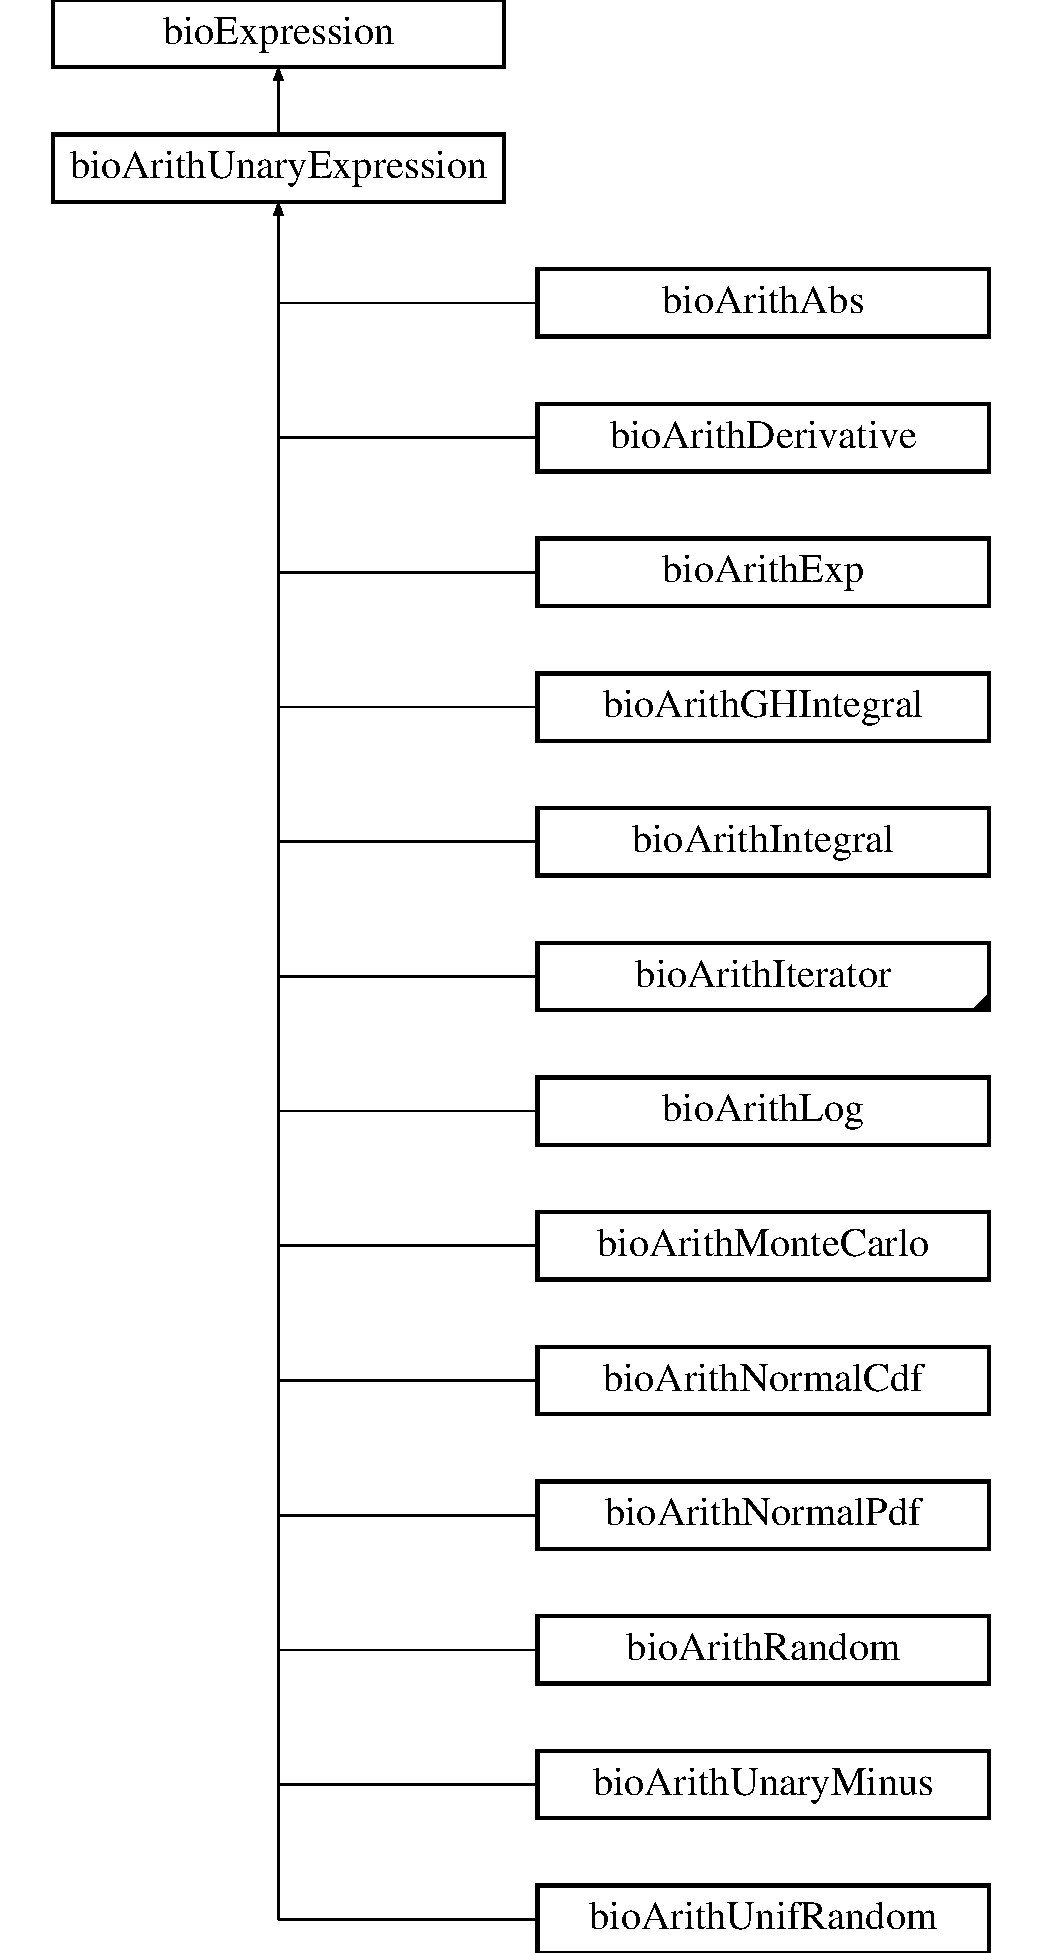
\includegraphics[height=12.000000cm]{classbio_arith_unary_expression}
\end{center}
\end{figure}
\subsection*{Public Member Functions}
\begin{DoxyCompactItemize}
\item 
\mbox{\Hypertarget{classbio_arith_unary_expression_ac8e8a90f5935ff89e5eff3d606b45f1a}\label{classbio_arith_unary_expression_ac8e8a90f5935ff89e5eff3d606b45f1a}} 
{\bfseries bio\+Arith\+Unary\+Expression} (\hyperlink{classbio_expression_repository}{bio\+Expression\+Repository} $\ast$rep, pat\+U\+Long par, pat\+U\+Long c, pat\+Error $\ast$\&err)
\item 
\mbox{\Hypertarget{classbio_arith_unary_expression_a9b3fb378875ca54fcbd70acf8f6ef7a9}\label{classbio_arith_unary_expression_a9b3fb378875ca54fcbd70acf8f6ef7a9}} 
virtual \hyperlink{classbio_expression}{bio\+Expression} $\ast$ {\bfseries get\+Child} () const
\item 
virtual pat\+String \hyperlink{classbio_arith_unary_expression_a974b7779804861f331a75e08db377926}{get\+Expression} (pat\+Error $\ast$\&err) const
\item 
\mbox{\Hypertarget{classbio_arith_unary_expression_ae40eb0f22afee1e6268d6f2a763c0d21}\label{classbio_arith_unary_expression_ae40eb0f22afee1e6268d6f2a763c0d21}} 
virtual pat\+U\+Long {\bfseries get\+Number\+Of\+Operations} () const
\item 
\mbox{\Hypertarget{classbio_arith_unary_expression_a128313ec9bd6f0ef6ebb5f8b67ccc477}\label{classbio_arith_unary_expression_a128313ec9bd6f0ef6ebb5f8b67ccc477}} 
virtual pat\+Boolean {\bfseries depends\+Of} (pat\+U\+Long a\+Literal\+Id) const
\item 
\mbox{\Hypertarget{classbio_arith_unary_expression_ade8b48b1ddca7299bca96c77d97bb8e9}\label{classbio_arith_unary_expression_ade8b48b1ddca7299bca96c77d97bb8e9}} 
virtual pat\+Boolean {\bfseries contains\+An\+Iterator} () const
\item 
\mbox{\Hypertarget{classbio_arith_unary_expression_aa8e5a9972f314f6051ad47cd7c892c84}\label{classbio_arith_unary_expression_aa8e5a9972f314f6051ad47cd7c892c84}} 
virtual pat\+Boolean {\bfseries contains\+An\+Iterator\+On\+Rows} () const
\item 
\mbox{\Hypertarget{classbio_arith_unary_expression_af93b8256cead1cb6ba632f360e78f1c2}\label{classbio_arith_unary_expression_af93b8256cead1cb6ba632f360e78f1c2}} 
virtual pat\+Boolean {\bfseries contains\+An\+Integral} () const
\item 
\mbox{\Hypertarget{classbio_arith_unary_expression_a2f99fbc5344f4610676d40883209a61c}\label{classbio_arith_unary_expression_a2f99fbc5344f4610676d40883209a61c}} 
virtual pat\+Boolean {\bfseries contains\+A\+Sequence} () const
\item 
\mbox{\Hypertarget{classbio_arith_unary_expression_a67153c2ecbab06a404d52fed92047fad}\label{classbio_arith_unary_expression_a67153c2ecbab06a404d52fed92047fad}} 
virtual void {\bfseries simplify\+Zeros} (pat\+Error $\ast$\&err)
\item 
\mbox{\Hypertarget{classbio_arith_unary_expression_a158beb11790272f8cd9438afe3b78ff2}\label{classbio_arith_unary_expression_a158beb11790272f8cd9438afe3b78ff2}} 
virtual void {\bfseries collect\+Expression\+Ids} (set$<$ pat\+U\+Long $>$ $\ast$s) const
\item 
\mbox{\Hypertarget{classbio_arith_unary_expression_a73cf4b2ffae2bd9af88ec72ec76c2043}\label{classbio_arith_unary_expression_a73cf4b2ffae2bd9af88ec72ec76c2043}} 
virtual pat\+String {\bfseries check} (pat\+Error $\ast$\&err) const
\end{DoxyCompactItemize}
\subsection*{Protected Attributes}
\begin{DoxyCompactItemize}
\item 
\mbox{\Hypertarget{classbio_arith_unary_expression_ad83897e3f655f2c25e603cc50249ac3a}\label{classbio_arith_unary_expression_ad83897e3f655f2c25e603cc50249ac3a}} 
pat\+U\+Long {\bfseries child\+Id}
\item 
\mbox{\Hypertarget{classbio_arith_unary_expression_a654eeff5056aaab7bfc8dd825feeeb6b}\label{classbio_arith_unary_expression_a654eeff5056aaab7bfc8dd825feeeb6b}} 
\hyperlink{classbio_expression}{bio\+Expression} $\ast$ {\bfseries child}
\end{DoxyCompactItemize}


\subsection{Detailed Description}
Class implementing a node of the tree representing a sum expression 

\subsection{Member Function Documentation}
\mbox{\Hypertarget{classbio_arith_unary_expression_a974b7779804861f331a75e08db377926}\label{classbio_arith_unary_expression_a974b7779804861f331a75e08db377926}} 
\index{bio\+Arith\+Unary\+Expression@{bio\+Arith\+Unary\+Expression}!get\+Expression@{get\+Expression}}
\index{get\+Expression@{get\+Expression}!bio\+Arith\+Unary\+Expression@{bio\+Arith\+Unary\+Expression}}
\subsubsection{\texorpdfstring{get\+Expression()}{getExpression()}}
{\footnotesize\ttfamily pat\+String bio\+Arith\+Unary\+Expression\+::get\+Expression (\begin{DoxyParamCaption}\item[{pat\+Error $\ast$\&}]{err }\end{DoxyParamCaption}) const\hspace{0.3cm}{\ttfamily [virtual]}}

\begin{DoxyReturn}{Returns}
printed expression 
\end{DoxyReturn}


Reimplemented from \hyperlink{classbio_expression_a66a83eb0caac18dd5e568ffde5a8b5d4}{bio\+Expression}.



Reimplemented in \hyperlink{classbio_arith_random_a54b48a4876469d44f324f73758ea1b6c}{bio\+Arith\+Random}, \hyperlink{classbio_arith_unif_random_a4c81af6983404929d1e06367f69a2256}{bio\+Arith\+Unif\+Random}, \hyperlink{classbio_arith_iterator_aceb6ee1a4c024349178de5edf4624710}{bio\+Arith\+Iterator}, and \hyperlink{classbio_arith_derivative_a5cdf6c4903ec8123b30c0d2ce059718d}{bio\+Arith\+Derivative}.



The documentation for this class was generated from the following files\+:\begin{DoxyCompactItemize}
\item 
bio\+Arith\+Unary\+Expression.\+h\item 
bio\+Arith\+Unary\+Expression.\+cc\end{DoxyCompactItemize}

\hypertarget{classbio_arith_unary_minus}{}\section{bio\+Arith\+Unary\+Minus Class Reference}
\label{classbio_arith_unary_minus}\index{bio\+Arith\+Unary\+Minus@{bio\+Arith\+Unary\+Minus}}


{\ttfamily \#include $<$bio\+Arith\+Unary\+Minus.\+h$>$}

Inheritance diagram for bio\+Arith\+Unary\+Minus\+:\begin{figure}[H]
\begin{center}
\leavevmode
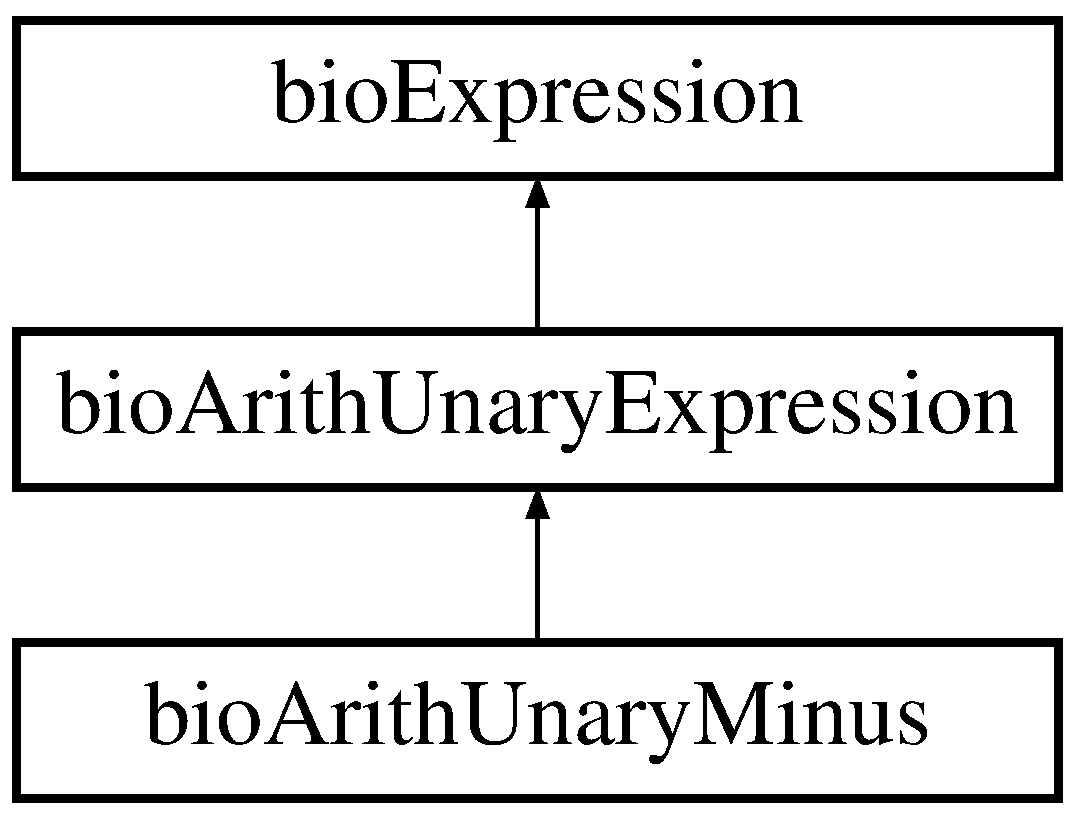
\includegraphics[height=3.000000cm]{classbio_arith_unary_minus}
\end{center}
\end{figure}
\subsection*{Public Member Functions}
\begin{DoxyCompactItemize}
\item 
\mbox{\Hypertarget{classbio_arith_unary_minus_aef0b0cea108500176219e8ab209012da}\label{classbio_arith_unary_minus_aef0b0cea108500176219e8ab209012da}} 
{\bfseries bio\+Arith\+Unary\+Minus} (\hyperlink{classbio_expression_repository}{bio\+Expression\+Repository} $\ast$rep, pat\+U\+Long par, pat\+U\+Long left, pat\+Error $\ast$\&err)
\item 
virtual pat\+String \hyperlink{classbio_arith_unary_minus_a59b3bcf198b25bc802775014bfce2f21}{get\+Operator\+Name} () const
\item 
virtual pat\+Real \hyperlink{classbio_arith_unary_minus_a0a31abb1d5a352b933c2d07cb2c657c8}{get\+Value} (pat\+Boolean prepare\+Gradient, pat\+U\+Long current\+Lap, pat\+Error $\ast$\&err)
\item 
virtual \hyperlink{classbio_expression}{bio\+Expression} $\ast$ \hyperlink{classbio_arith_unary_minus_aaf1b155993a12037850b1a22dbb36f7c}{get\+Derivative} (pat\+U\+Long a\+Literal\+Id, pat\+Error $\ast$\&err) const
\item 
virtual \hyperlink{classbio_arith_unary_minus}{bio\+Arith\+Unary\+Minus} $\ast$ \hyperlink{classbio_arith_unary_minus_a1bd7f28b742866f8a8e84b5f8405fbd1}{get\+Deep\+Copy} (\hyperlink{classbio_expression_repository}{bio\+Expression\+Repository} $\ast$rep, pat\+Error $\ast$\&err) const
\item 
virtual \hyperlink{classbio_arith_unary_minus}{bio\+Arith\+Unary\+Minus} $\ast$ \hyperlink{classbio_arith_unary_minus_af7d31f14e0e619536f33c45fedb7fa79}{get\+Shallow\+Copy} (\hyperlink{classbio_expression_repository}{bio\+Expression\+Repository} $\ast$rep, pat\+Error $\ast$\&err) const
\item 
virtual pat\+String \hyperlink{classbio_arith_unary_minus_a2e8b40486ef897c00ce5a99e7f8ebd03}{get\+Expression\+String} () const
\item 
virtual \hyperlink{classbio_function_and_derivatives}{bio\+Function\+And\+Derivatives} $\ast$ \hyperlink{classbio_arith_unary_minus_a8fc3f51f45b38f8e710db12eec18b9fb}{get\+Numerical\+Function\+And\+Gradient} (vector$<$ pat\+U\+Long $>$ literal\+Ids, pat\+Boolean compute\+Hessian, pat\+Boolean debug\+Derivatives, pat\+Error $\ast$\&err)
\end{DoxyCompactItemize}
\subsection*{Additional Inherited Members}


\subsection{Detailed Description}
Class implementing a node of the tree representing a unary minus operation 

\subsection{Member Function Documentation}
\mbox{\Hypertarget{classbio_arith_unary_minus_a1bd7f28b742866f8a8e84b5f8405fbd1}\label{classbio_arith_unary_minus_a1bd7f28b742866f8a8e84b5f8405fbd1}} 
\index{bio\+Arith\+Unary\+Minus@{bio\+Arith\+Unary\+Minus}!get\+Deep\+Copy@{get\+Deep\+Copy}}
\index{get\+Deep\+Copy@{get\+Deep\+Copy}!bio\+Arith\+Unary\+Minus@{bio\+Arith\+Unary\+Minus}}
\subsubsection{\texorpdfstring{get\+Deep\+Copy()}{getDeepCopy()}}
{\footnotesize\ttfamily \hyperlink{classbio_arith_unary_minus}{bio\+Arith\+Unary\+Minus} $\ast$ bio\+Arith\+Unary\+Minus\+::get\+Deep\+Copy (\begin{DoxyParamCaption}\item[{\hyperlink{classbio_expression_repository}{bio\+Expression\+Repository} $\ast$}]{rep,  }\item[{pat\+Error $\ast$\&}]{err }\end{DoxyParamCaption}) const\hspace{0.3cm}{\ttfamily [virtual]}}

Create a deep copy of the expression and returns a pointer to it. It means that new instances of the children are created. 

Reimplemented from \hyperlink{classbio_expression_a4ee1b8add634078a02eaae26cd40dcc8}{bio\+Expression}.

\mbox{\Hypertarget{classbio_arith_unary_minus_aaf1b155993a12037850b1a22dbb36f7c}\label{classbio_arith_unary_minus_aaf1b155993a12037850b1a22dbb36f7c}} 
\index{bio\+Arith\+Unary\+Minus@{bio\+Arith\+Unary\+Minus}!get\+Derivative@{get\+Derivative}}
\index{get\+Derivative@{get\+Derivative}!bio\+Arith\+Unary\+Minus@{bio\+Arith\+Unary\+Minus}}
\subsubsection{\texorpdfstring{get\+Derivative()}{getDerivative()}}
{\footnotesize\ttfamily \hyperlink{classbio_expression}{bio\+Expression} $\ast$ bio\+Arith\+Unary\+Minus\+::get\+Derivative (\begin{DoxyParamCaption}\item[{pat\+U\+Long}]{a\+Literal\+Id,  }\item[{pat\+Error $\ast$\&}]{err }\end{DoxyParamCaption}) const\hspace{0.3cm}{\ttfamily [virtual]}}

\begin{DoxyReturn}{Returns}
value of the derivative w.\+r.\+t literal 
\end{DoxyReturn}

\begin{DoxyParams}{Parameters}
{\em index} & of the literal involved in the derivative \\
\hline
{\em err} & ref. of the pointer to the error object. \\
\hline
\end{DoxyParams}


Reimplemented from \hyperlink{classbio_expression_a5915579d1193f25f216c1e273c97f2ce}{bio\+Expression}.

\mbox{\Hypertarget{classbio_arith_unary_minus_a2e8b40486ef897c00ce5a99e7f8ebd03}\label{classbio_arith_unary_minus_a2e8b40486ef897c00ce5a99e7f8ebd03}} 
\index{bio\+Arith\+Unary\+Minus@{bio\+Arith\+Unary\+Minus}!get\+Expression\+String@{get\+Expression\+String}}
\index{get\+Expression\+String@{get\+Expression\+String}!bio\+Arith\+Unary\+Minus@{bio\+Arith\+Unary\+Minus}}
\subsubsection{\texorpdfstring{get\+Expression\+String()}{getExpressionString()}}
{\footnotesize\ttfamily pat\+String bio\+Arith\+Unary\+Minus\+::get\+Expression\+String (\begin{DoxyParamCaption}{ }\end{DoxyParamCaption}) const\hspace{0.3cm}{\ttfamily [virtual]}}

Compute a string that represents the expression. It is designed to replace the expression itself when used only for comparison purposes. Code\+: +\{expr1\}\{expr2\}\+: binary plus -\/\{expr1\}\{expr2\}\+: binary minus \{expr1\}\{expr2\}\+: multiplication /\{expr1\}\{expr2\}\+: division $^\wedge$\{expr1\}\{expr2\}\+: power \&\{expr1\}\{expr2\}\+: and $\vert$\{expr1\}\{expr2\}\+: or =\{expr1\}\{expr2\}\+: equal !=\{expr1\}\{expr2\}\+: not equal $<$\{expr1\}\{expr2\}\+: lesser than $<$=\{expr1\}\{expr2\}\+: lesser or equal to $>$\{expr1\}\{expr2\}\+: greater than $>$=\{expr1\}\{expr2\}\+: greater or equal to \$A\{expr\}\+: abs \$D\mbox{[}expr\mbox{]}\mbox{[}\{expr1\}...\{exprN\}\mbox{]}\+: dictionary (\hyperlink{classbio_arith_elem}{bio\+Arith\+Elem}) \$E\{expr\}\+: exp \$L\{expr\}\+: log \$M\{expr\}\+: Unary minus \$\+Piterator\+\_\+name\{expr\}\+: prod \$Q\{string1\}\{string2\}\+: sequence \$\+Siterator\+\_\+name\{expr\}\+: sum \$\+Ziterator\+\_\+name\mbox{[}\{expr1\}...\{exprN\}\mbox{]}\+: merged sum \{expr1\}\{expr2\}...\{exprN\}//\+: list of expressions number\+: constant \#id\+: literal \&id\+: random 

Reimplemented from \hyperlink{classbio_expression_a3e4b4dca58dbbc6f0e411b30eb3f60b4}{bio\+Expression}.

\mbox{\Hypertarget{classbio_arith_unary_minus_a8fc3f51f45b38f8e710db12eec18b9fb}\label{classbio_arith_unary_minus_a8fc3f51f45b38f8e710db12eec18b9fb}} 
\index{bio\+Arith\+Unary\+Minus@{bio\+Arith\+Unary\+Minus}!get\+Numerical\+Function\+And\+Gradient@{get\+Numerical\+Function\+And\+Gradient}}
\index{get\+Numerical\+Function\+And\+Gradient@{get\+Numerical\+Function\+And\+Gradient}!bio\+Arith\+Unary\+Minus@{bio\+Arith\+Unary\+Minus}}
\subsubsection{\texorpdfstring{get\+Numerical\+Function\+And\+Gradient()}{getNumericalFunctionAndGradient()}}
{\footnotesize\ttfamily \hyperlink{classbio_function_and_derivatives}{bio\+Function\+And\+Derivatives} $\ast$ bio\+Arith\+Unary\+Minus\+::get\+Numerical\+Function\+And\+Gradient (\begin{DoxyParamCaption}\item[{vector$<$ pat\+U\+Long $>$}]{literal\+Ids,  }\item[{pat\+Boolean}]{compute\+Hessian,  }\item[{pat\+Boolean}]{debug\+Derivatives,  }\item[{pat\+Error $\ast$\&}]{err }\end{DoxyParamCaption})\hspace{0.3cm}{\ttfamily [virtual]}}

\begin{DoxyReturn}{Returns}
value and gradient of the expression 
\end{DoxyReturn}

\begin{DoxyParams}{Parameters}
{\em err} & ref. of the pointer to the error object. \\
\hline
\end{DoxyParams}


Reimplemented from \hyperlink{classbio_expression_a91c81ce80c9e972c913b10f5f3c1ed13}{bio\+Expression}.

\mbox{\Hypertarget{classbio_arith_unary_minus_a59b3bcf198b25bc802775014bfce2f21}\label{classbio_arith_unary_minus_a59b3bcf198b25bc802775014bfce2f21}} 
\index{bio\+Arith\+Unary\+Minus@{bio\+Arith\+Unary\+Minus}!get\+Operator\+Name@{get\+Operator\+Name}}
\index{get\+Operator\+Name@{get\+Operator\+Name}!bio\+Arith\+Unary\+Minus@{bio\+Arith\+Unary\+Minus}}
\subsubsection{\texorpdfstring{get\+Operator\+Name()}{getOperatorName()}}
{\footnotesize\ttfamily pat\+String bio\+Arith\+Unary\+Minus\+::get\+Operator\+Name (\begin{DoxyParamCaption}{ }\end{DoxyParamCaption}) const\hspace{0.3cm}{\ttfamily [virtual]}}

\begin{DoxyReturn}{Returns}
name of the operator 
\end{DoxyReturn}


Reimplemented from \hyperlink{classbio_expression_a2353a4afb3a2b0af7c63aba086a72bde}{bio\+Expression}.

\mbox{\Hypertarget{classbio_arith_unary_minus_af7d31f14e0e619536f33c45fedb7fa79}\label{classbio_arith_unary_minus_af7d31f14e0e619536f33c45fedb7fa79}} 
\index{bio\+Arith\+Unary\+Minus@{bio\+Arith\+Unary\+Minus}!get\+Shallow\+Copy@{get\+Shallow\+Copy}}
\index{get\+Shallow\+Copy@{get\+Shallow\+Copy}!bio\+Arith\+Unary\+Minus@{bio\+Arith\+Unary\+Minus}}
\subsubsection{\texorpdfstring{get\+Shallow\+Copy()}{getShallowCopy()}}
{\footnotesize\ttfamily \hyperlink{classbio_arith_unary_minus}{bio\+Arith\+Unary\+Minus} $\ast$ bio\+Arith\+Unary\+Minus\+::get\+Shallow\+Copy (\begin{DoxyParamCaption}\item[{\hyperlink{classbio_expression_repository}{bio\+Expression\+Repository} $\ast$}]{rep,  }\item[{pat\+Error $\ast$\&}]{err }\end{DoxyParamCaption}) const\hspace{0.3cm}{\ttfamily [virtual]}}

Create a shallow copy of the expression and returns a pointer to it. It means that no new instance of the children are created. It is typically called by the repository 

Reimplemented from \hyperlink{classbio_expression_a442534762693b92baaf33928979a1bf8}{bio\+Expression}.

\mbox{\Hypertarget{classbio_arith_unary_minus_a0a31abb1d5a352b933c2d07cb2c657c8}\label{classbio_arith_unary_minus_a0a31abb1d5a352b933c2d07cb2c657c8}} 
\index{bio\+Arith\+Unary\+Minus@{bio\+Arith\+Unary\+Minus}!get\+Value@{get\+Value}}
\index{get\+Value@{get\+Value}!bio\+Arith\+Unary\+Minus@{bio\+Arith\+Unary\+Minus}}
\subsubsection{\texorpdfstring{get\+Value()}{getValue()}}
{\footnotesize\ttfamily pat\+Real bio\+Arith\+Unary\+Minus\+::get\+Value (\begin{DoxyParamCaption}\item[{pat\+Boolean}]{prepare\+Gradient,  }\item[{pat\+U\+Long}]{current\+Lap,  }\item[{pat\+Error $\ast$\&}]{err }\end{DoxyParamCaption})\hspace{0.3cm}{\ttfamily [virtual]}}

\begin{DoxyReturn}{Returns}
value of the expression 
\end{DoxyReturn}

\begin{DoxyParams}{Parameters}
{\em err} & ref. of the pointer to the error object. \\
\hline
\end{DoxyParams}


Reimplemented from \hyperlink{classbio_expression_af58662a5d4d456f15bc4f2c9bd4f8a5b}{bio\+Expression}.



The documentation for this class was generated from the following files\+:\begin{DoxyCompactItemize}
\item 
bio\+Arith\+Unary\+Minus.\+h\item 
bio\+Arith\+Unary\+Minus.\+cc\end{DoxyCompactItemize}

\hypertarget{classbio_arith_unif_random}{}\section{bio\+Arith\+Unif\+Random Class Reference}
\label{classbio_arith_unif_random}\index{bio\+Arith\+Unif\+Random@{bio\+Arith\+Unif\+Random}}


{\ttfamily \#include $<$bio\+Arith\+Unif\+Random.\+h$>$}

Inheritance diagram for bio\+Arith\+Unif\+Random\+:\begin{figure}[H]
\begin{center}
\leavevmode
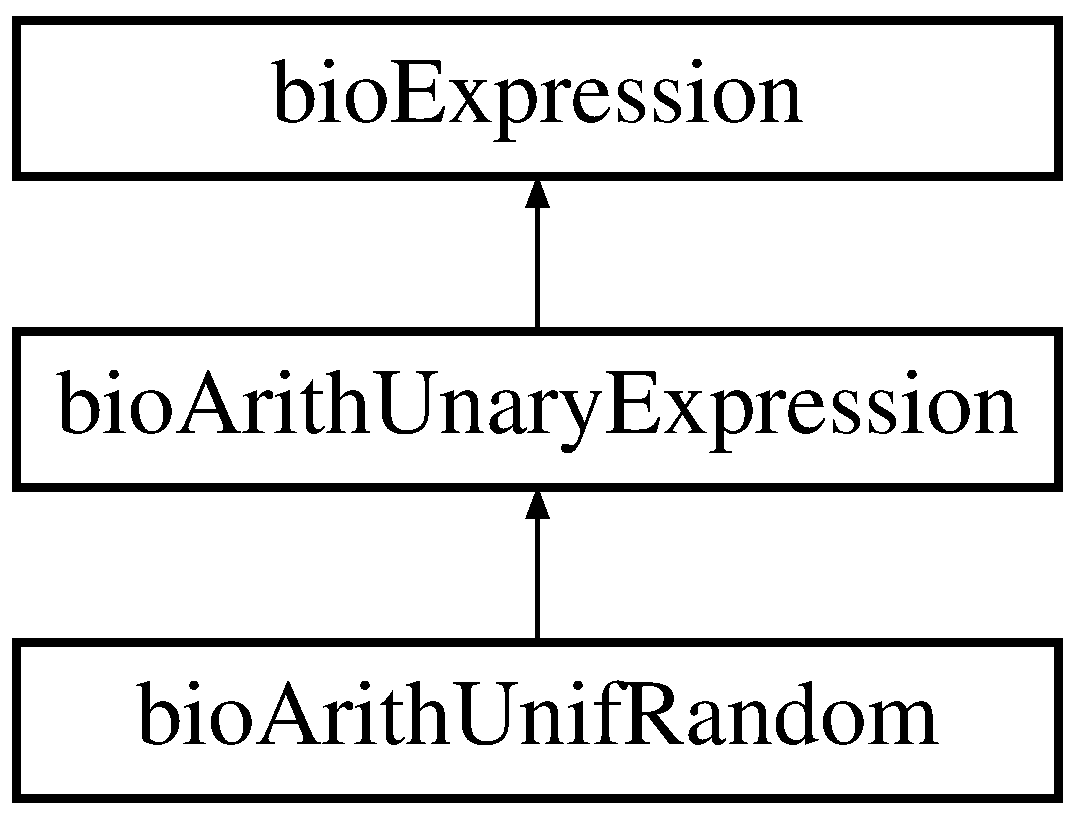
\includegraphics[height=3.000000cm]{classbio_arith_unif_random}
\end{center}
\end{figure}
\subsection*{Public Member Functions}
\begin{DoxyCompactItemize}
\item 
\mbox{\Hypertarget{classbio_arith_unif_random_a0d73002a7576849dc2233b79d26248f6}\label{classbio_arith_unif_random_a0d73002a7576849dc2233b79d26248f6}} 
{\bfseries bio\+Arith\+Unif\+Random} (\hyperlink{classbio_expression_repository}{bio\+Expression\+Repository} $\ast$rep, pat\+U\+Long par, pat\+U\+Long individual, pat\+U\+Long id, bio\+Random\+Draws\+::bio\+Draws\+Type type, pat\+Error $\ast$\&err)
\item 
pat\+String \hyperlink{classbio_arith_unif_random_acd356155220e3b8cbc5d1580e1ec0f47}{get\+Operator\+Name} () const
\item 
virtual pat\+Real \hyperlink{classbio_arith_unif_random_adf48d57d0dc6d518950c58dc13b65a32}{get\+Value} (pat\+Boolean prepare\+Gradient, pat\+U\+Long current\+Lap, pat\+Error $\ast$\&err)
\item 
\hyperlink{classbio_expression}{bio\+Expression} $\ast$ \hyperlink{classbio_arith_unif_random_ab235d1b207d96e122b5b595ddeb70a68}{get\+Derivative} (pat\+U\+Long a\+Literal\+Id, pat\+Error $\ast$\&err) const
\item 
\hyperlink{classbio_arith_unif_random}{bio\+Arith\+Unif\+Random} $\ast$ \hyperlink{classbio_arith_unif_random_ad7aaa2ab5f06eb38945d39359bb55df5}{get\+Deep\+Copy} (\hyperlink{classbio_expression_repository}{bio\+Expression\+Repository} $\ast$rep, pat\+Error $\ast$\&err) const
\item 
\hyperlink{classbio_arith_unif_random}{bio\+Arith\+Unif\+Random} $\ast$ \hyperlink{classbio_arith_unif_random_a8e81dcec495449b481729aa3769696ad}{get\+Shallow\+Copy} (\hyperlink{classbio_expression_repository}{bio\+Expression\+Repository} $\ast$rep, pat\+Error $\ast$\&err) const
\item 
\mbox{\Hypertarget{classbio_arith_unif_random_a2b641a7dd14bea4132412192ea8abbeb}\label{classbio_arith_unif_random_a2b641a7dd14bea4132412192ea8abbeb}} 
pat\+U\+Long {\bfseries get\+Number\+Of\+Operations} () const
\item 
pat\+String \hyperlink{classbio_arith_unif_random_a5d53c24c5b584c9ce817c6140b3e6001}{get\+Expression\+String} () const
\item 
pat\+String \hyperlink{classbio_arith_unif_random_a4c81af6983404929d1e06367f69a2256}{get\+Expression} (pat\+Error $\ast$\&err) const
\item 
\mbox{\Hypertarget{classbio_arith_unif_random_ae0cc538b07be9f3a79c9716dd2898db8}\label{classbio_arith_unif_random_ae0cc538b07be9f3a79c9716dd2898db8}} 
pat\+Boolean {\bfseries depends\+Of} (pat\+U\+Long a\+Literal\+Id) const
\item 
virtual \hyperlink{classbio_function_and_derivatives}{bio\+Function\+And\+Derivatives} $\ast$ \hyperlink{classbio_arith_unif_random_a0a5860c93f0efaea7f448d44f76cae60}{get\+Numerical\+Function\+And\+Gradient} (vector$<$ pat\+U\+Long $>$ literal\+Ids, pat\+Boolean compute\+Hessian, pat\+Boolean debug\+Derivatives, pat\+Error $\ast$\&err)
\end{DoxyCompactItemize}
\subsection*{Protected Attributes}
\begin{DoxyCompactItemize}
\item 
\mbox{\Hypertarget{classbio_arith_unif_random_a0d448466887276155422c56cfa9d12ae}\label{classbio_arith_unif_random_a0d448466887276155422c56cfa9d12ae}} 
pat\+U\+Long {\bfseries variable\+Id\+For\+Draws}
\item 
\mbox{\Hypertarget{classbio_arith_unif_random_af342ff300e284db90f92bfd8c31b5609}\label{classbio_arith_unif_random_af342ff300e284db90f92bfd8c31b5609}} 
bio\+Random\+Draws\+::bio\+Draws\+Type {\bfseries type}
\end{DoxyCompactItemize}


\subsection{Detailed Description}
Class defining an interface for a random parameter uusing draws 

\subsection{Member Function Documentation}
\mbox{\Hypertarget{classbio_arith_unif_random_ad7aaa2ab5f06eb38945d39359bb55df5}\label{classbio_arith_unif_random_ad7aaa2ab5f06eb38945d39359bb55df5}} 
\index{bio\+Arith\+Unif\+Random@{bio\+Arith\+Unif\+Random}!get\+Deep\+Copy@{get\+Deep\+Copy}}
\index{get\+Deep\+Copy@{get\+Deep\+Copy}!bio\+Arith\+Unif\+Random@{bio\+Arith\+Unif\+Random}}
\subsubsection{\texorpdfstring{get\+Deep\+Copy()}{getDeepCopy()}}
{\footnotesize\ttfamily \hyperlink{classbio_arith_unif_random}{bio\+Arith\+Unif\+Random} $\ast$ bio\+Arith\+Unif\+Random\+::get\+Deep\+Copy (\begin{DoxyParamCaption}\item[{\hyperlink{classbio_expression_repository}{bio\+Expression\+Repository} $\ast$}]{rep,  }\item[{pat\+Error $\ast$\&}]{err }\end{DoxyParamCaption}) const\hspace{0.3cm}{\ttfamily [virtual]}}

Create a deep copy of the expression and returns a pointer to it. It means that new instances of the children are created. 

Reimplemented from \hyperlink{classbio_expression_a4ee1b8add634078a02eaae26cd40dcc8}{bio\+Expression}.

\mbox{\Hypertarget{classbio_arith_unif_random_ab235d1b207d96e122b5b595ddeb70a68}\label{classbio_arith_unif_random_ab235d1b207d96e122b5b595ddeb70a68}} 
\index{bio\+Arith\+Unif\+Random@{bio\+Arith\+Unif\+Random}!get\+Derivative@{get\+Derivative}}
\index{get\+Derivative@{get\+Derivative}!bio\+Arith\+Unif\+Random@{bio\+Arith\+Unif\+Random}}
\subsubsection{\texorpdfstring{get\+Derivative()}{getDerivative()}}
{\footnotesize\ttfamily \hyperlink{classbio_expression}{bio\+Expression} $\ast$ bio\+Arith\+Unif\+Random\+::get\+Derivative (\begin{DoxyParamCaption}\item[{pat\+U\+Long}]{a\+Literal\+Id,  }\item[{pat\+Error $\ast$\&}]{err }\end{DoxyParamCaption}) const\hspace{0.3cm}{\ttfamily [virtual]}}

\begin{DoxyReturn}{Returns}
value of the derivative w.\+r.\+t literal 
\end{DoxyReturn}

\begin{DoxyParams}{Parameters}
{\em index} & of the literal involved in the derivative \\
\hline
{\em err} & ref. of the pointer to the error object. \\
\hline
\end{DoxyParams}


Reimplemented from \hyperlink{classbio_expression_a5915579d1193f25f216c1e273c97f2ce}{bio\+Expression}.

\mbox{\Hypertarget{classbio_arith_unif_random_a4c81af6983404929d1e06367f69a2256}\label{classbio_arith_unif_random_a4c81af6983404929d1e06367f69a2256}} 
\index{bio\+Arith\+Unif\+Random@{bio\+Arith\+Unif\+Random}!get\+Expression@{get\+Expression}}
\index{get\+Expression@{get\+Expression}!bio\+Arith\+Unif\+Random@{bio\+Arith\+Unif\+Random}}
\subsubsection{\texorpdfstring{get\+Expression()}{getExpression()}}
{\footnotesize\ttfamily pat\+String bio\+Arith\+Unif\+Random\+::get\+Expression (\begin{DoxyParamCaption}\item[{pat\+Error $\ast$\&}]{err }\end{DoxyParamCaption}) const\hspace{0.3cm}{\ttfamily [virtual]}}

\begin{DoxyReturn}{Returns}
printed expression 
\end{DoxyReturn}


Reimplemented from \hyperlink{classbio_arith_unary_expression_a974b7779804861f331a75e08db377926}{bio\+Arith\+Unary\+Expression}.

\mbox{\Hypertarget{classbio_arith_unif_random_a5d53c24c5b584c9ce817c6140b3e6001}\label{classbio_arith_unif_random_a5d53c24c5b584c9ce817c6140b3e6001}} 
\index{bio\+Arith\+Unif\+Random@{bio\+Arith\+Unif\+Random}!get\+Expression\+String@{get\+Expression\+String}}
\index{get\+Expression\+String@{get\+Expression\+String}!bio\+Arith\+Unif\+Random@{bio\+Arith\+Unif\+Random}}
\subsubsection{\texorpdfstring{get\+Expression\+String()}{getExpressionString()}}
{\footnotesize\ttfamily pat\+String bio\+Arith\+Unif\+Random\+::get\+Expression\+String (\begin{DoxyParamCaption}{ }\end{DoxyParamCaption}) const\hspace{0.3cm}{\ttfamily [virtual]}}

Compute a string that represents the expression. It is designed to replace the expression itself when used only for comparison purposes. Code\+: +\{expr1\}\{expr2\}\+: binary plus -\/\{expr1\}\{expr2\}\+: binary minus \{expr1\}\{expr2\}\+: multiplication /\{expr1\}\{expr2\}\+: division $^\wedge$\{expr1\}\{expr2\}\+: power \&\{expr1\}\{expr2\}\+: and $\vert$\{expr1\}\{expr2\}\+: or =\{expr1\}\{expr2\}\+: equal !=\{expr1\}\{expr2\}\+: not equal $<$\{expr1\}\{expr2\}\+: lesser than $<$=\{expr1\}\{expr2\}\+: lesser or equal to $>$\{expr1\}\{expr2\}\+: greater than $>$=\{expr1\}\{expr2\}\+: greater or equal to \$A\{expr\}\+: abs \$D\mbox{[}expr\mbox{]}\mbox{[}\{expr1\}...\{exprN\}\mbox{]}\+: dictionary (\hyperlink{classbio_arith_elem}{bio\+Arith\+Elem}) \$E\{expr\}\+: exp \$L\{expr\}\+: log \$M\{expr\}\+: Unary minus \$\+Piterator\+\_\+name\{expr\}\+: prod \$Q\{string1\}\{string2\}\+: sequence \$\+Siterator\+\_\+name\{expr\}\+: sum \$\+Ziterator\+\_\+name\mbox{[}\{expr1\}...\{exprN\}\mbox{]}\+: merged sum \{expr1\}\{expr2\}...\{exprN\}//\+: list of expressions number\+: constant \#id\+: literal \&id\+: random 

Reimplemented from \hyperlink{classbio_expression_a3e4b4dca58dbbc6f0e411b30eb3f60b4}{bio\+Expression}.

\mbox{\Hypertarget{classbio_arith_unif_random_a0a5860c93f0efaea7f448d44f76cae60}\label{classbio_arith_unif_random_a0a5860c93f0efaea7f448d44f76cae60}} 
\index{bio\+Arith\+Unif\+Random@{bio\+Arith\+Unif\+Random}!get\+Numerical\+Function\+And\+Gradient@{get\+Numerical\+Function\+And\+Gradient}}
\index{get\+Numerical\+Function\+And\+Gradient@{get\+Numerical\+Function\+And\+Gradient}!bio\+Arith\+Unif\+Random@{bio\+Arith\+Unif\+Random}}
\subsubsection{\texorpdfstring{get\+Numerical\+Function\+And\+Gradient()}{getNumericalFunctionAndGradient()}}
{\footnotesize\ttfamily \hyperlink{classbio_function_and_derivatives}{bio\+Function\+And\+Derivatives} $\ast$ bio\+Arith\+Unif\+Random\+::get\+Numerical\+Function\+And\+Gradient (\begin{DoxyParamCaption}\item[{vector$<$ pat\+U\+Long $>$}]{literal\+Ids,  }\item[{pat\+Boolean}]{compute\+Hessian,  }\item[{pat\+Boolean}]{debug\+Derivatives,  }\item[{pat\+Error $\ast$\&}]{err }\end{DoxyParamCaption})\hspace{0.3cm}{\ttfamily [virtual]}}

\begin{DoxyReturn}{Returns}
value and gradient of the expression 
\end{DoxyReturn}

\begin{DoxyParams}{Parameters}
{\em err} & ref. of the pointer to the error object. \\
\hline
\end{DoxyParams}


Reimplemented from \hyperlink{classbio_expression_a91c81ce80c9e972c913b10f5f3c1ed13}{bio\+Expression}.

\mbox{\Hypertarget{classbio_arith_unif_random_acd356155220e3b8cbc5d1580e1ec0f47}\label{classbio_arith_unif_random_acd356155220e3b8cbc5d1580e1ec0f47}} 
\index{bio\+Arith\+Unif\+Random@{bio\+Arith\+Unif\+Random}!get\+Operator\+Name@{get\+Operator\+Name}}
\index{get\+Operator\+Name@{get\+Operator\+Name}!bio\+Arith\+Unif\+Random@{bio\+Arith\+Unif\+Random}}
\subsubsection{\texorpdfstring{get\+Operator\+Name()}{getOperatorName()}}
{\footnotesize\ttfamily pat\+String bio\+Arith\+Unif\+Random\+::get\+Operator\+Name (\begin{DoxyParamCaption}{ }\end{DoxyParamCaption}) const\hspace{0.3cm}{\ttfamily [virtual]}}

\begin{DoxyReturn}{Returns}
name of the operator 
\end{DoxyReturn}


Reimplemented from \hyperlink{classbio_expression_a2353a4afb3a2b0af7c63aba086a72bde}{bio\+Expression}.

\mbox{\Hypertarget{classbio_arith_unif_random_a8e81dcec495449b481729aa3769696ad}\label{classbio_arith_unif_random_a8e81dcec495449b481729aa3769696ad}} 
\index{bio\+Arith\+Unif\+Random@{bio\+Arith\+Unif\+Random}!get\+Shallow\+Copy@{get\+Shallow\+Copy}}
\index{get\+Shallow\+Copy@{get\+Shallow\+Copy}!bio\+Arith\+Unif\+Random@{bio\+Arith\+Unif\+Random}}
\subsubsection{\texorpdfstring{get\+Shallow\+Copy()}{getShallowCopy()}}
{\footnotesize\ttfamily \hyperlink{classbio_arith_unif_random}{bio\+Arith\+Unif\+Random} $\ast$ bio\+Arith\+Unif\+Random\+::get\+Shallow\+Copy (\begin{DoxyParamCaption}\item[{\hyperlink{classbio_expression_repository}{bio\+Expression\+Repository} $\ast$}]{rep,  }\item[{pat\+Error $\ast$\&}]{err }\end{DoxyParamCaption}) const\hspace{0.3cm}{\ttfamily [virtual]}}

Create a shallow copy of the expression and returns a pointer to it. It means that no new instance of the children are created. It is typically called by the repository 

Reimplemented from \hyperlink{classbio_expression_a442534762693b92baaf33928979a1bf8}{bio\+Expression}.

\mbox{\Hypertarget{classbio_arith_unif_random_adf48d57d0dc6d518950c58dc13b65a32}\label{classbio_arith_unif_random_adf48d57d0dc6d518950c58dc13b65a32}} 
\index{bio\+Arith\+Unif\+Random@{bio\+Arith\+Unif\+Random}!get\+Value@{get\+Value}}
\index{get\+Value@{get\+Value}!bio\+Arith\+Unif\+Random@{bio\+Arith\+Unif\+Random}}
\subsubsection{\texorpdfstring{get\+Value()}{getValue()}}
{\footnotesize\ttfamily pat\+Real bio\+Arith\+Unif\+Random\+::get\+Value (\begin{DoxyParamCaption}\item[{pat\+Boolean}]{prepare\+Gradient,  }\item[{pat\+U\+Long}]{current\+Lap,  }\item[{pat\+Error $\ast$\&}]{err }\end{DoxyParamCaption})\hspace{0.3cm}{\ttfamily [virtual]}}

\begin{DoxyReturn}{Returns}
value of the expression 
\end{DoxyReturn}

\begin{DoxyParams}{Parameters}
{\em err} & ref. of the pointer to the error object. \\
\hline
\end{DoxyParams}


Reimplemented from \hyperlink{classbio_expression_af58662a5d4d456f15bc4f2c9bd4f8a5b}{bio\+Expression}.



The documentation for this class was generated from the following files\+:\begin{DoxyCompactItemize}
\item 
bio\+Arith\+Unif\+Random.\+h\item 
bio\+Arith\+Unif\+Random.\+cc\end{DoxyCompactItemize}

\hypertarget{classbio_arith_variable}{}\section{bio\+Arith\+Variable Class Reference}
\label{classbio_arith_variable}\index{bio\+Arith\+Variable@{bio\+Arith\+Variable}}


{\ttfamily \#include $<$bio\+Arith\+Variable.\+h$>$}

Inheritance diagram for bio\+Arith\+Variable\+:\begin{figure}[H]
\begin{center}
\leavevmode
\includegraphics[height=4.000000cm]{classbio_arith_variable}
\end{center}
\end{figure}
\subsection*{Public Member Functions}
\begin{DoxyCompactItemize}
\item 
\mbox{\Hypertarget{classbio_arith_variable_aea4a29d0ed4f912e08020ba89356ab81}\label{classbio_arith_variable_aea4a29d0ed4f912e08020ba89356ab81}} 
{\bfseries bio\+Arith\+Variable} (\hyperlink{classbio_expression_repository}{bio\+Expression\+Repository} $\ast$rep, pat\+U\+Long par, pat\+U\+Long unique\+Id, pat\+U\+Long v\+Id)
\item 
virtual \hyperlink{classbio_arith_variable}{bio\+Arith\+Variable} $\ast$ \hyperlink{classbio_arith_variable_a13698945a07c98905254d7e773555de3}{get\+Deep\+Copy} (\hyperlink{classbio_expression_repository}{bio\+Expression\+Repository} $\ast$rep, pat\+Error $\ast$\&err) const
\item 
virtual \hyperlink{classbio_arith_variable}{bio\+Arith\+Variable} $\ast$ \hyperlink{classbio_arith_variable_a5b2185aabcab07bcd474479f8ca7dd94}{get\+Shallow\+Copy} (\hyperlink{classbio_expression_repository}{bio\+Expression\+Repository} $\ast$rep, pat\+Error $\ast$\&err) const
\item 
virtual pat\+Real \hyperlink{classbio_arith_variable_a49717d281e84536b65a715918fdfc4c5}{get\+Value} (pat\+Boolean prepare\+Gradient, pat\+U\+Long current\+Lap, pat\+Error $\ast$\&err)
\end{DoxyCompactItemize}
\subsection*{Protected Attributes}
\begin{DoxyCompactItemize}
\item 
\mbox{\Hypertarget{classbio_arith_variable_a723d43aeb4f13c31be658e181770e93f}\label{classbio_arith_variable_a723d43aeb4f13c31be658e181770e93f}} 
pat\+U\+Long {\bfseries the\+Variable\+Id}
\item 
\mbox{\Hypertarget{classbio_arith_variable_a12802d4fe378cf5cbac37d0723ee23a8}\label{classbio_arith_variable_a12802d4fe378cf5cbac37d0723ee23a8}} 
const \hyperlink{classbio_variable}{bio\+Variable} $\ast$ {\bfseries the\+Variable}
\item 
\mbox{\Hypertarget{classbio_arith_variable_a1653f23f7a3d6b1ad30117e536aad255}\label{classbio_arith_variable_a1653f23f7a3d6b1ad30117e536aad255}} 
pat\+Boolean {\bfseries check\+For\+Missing\+Values}
\item 
\mbox{\Hypertarget{classbio_arith_variable_a1b5e076f79e9ef016ba640b1399c5577}\label{classbio_arith_variable_a1b5e076f79e9ef016ba640b1399c5577}} 
pat\+Real {\bfseries missing\+Value}
\end{DoxyCompactItemize}


\subsection{Detailed Description}
Class implementing the node for variables in an expression 

\subsection{Member Function Documentation}
\mbox{\Hypertarget{classbio_arith_variable_a13698945a07c98905254d7e773555de3}\label{classbio_arith_variable_a13698945a07c98905254d7e773555de3}} 
\index{bio\+Arith\+Variable@{bio\+Arith\+Variable}!get\+Deep\+Copy@{get\+Deep\+Copy}}
\index{get\+Deep\+Copy@{get\+Deep\+Copy}!bio\+Arith\+Variable@{bio\+Arith\+Variable}}
\subsubsection{\texorpdfstring{get\+Deep\+Copy()}{getDeepCopy()}}
{\footnotesize\ttfamily \hyperlink{classbio_arith_variable}{bio\+Arith\+Variable} $\ast$ bio\+Arith\+Variable\+::get\+Deep\+Copy (\begin{DoxyParamCaption}\item[{\hyperlink{classbio_expression_repository}{bio\+Expression\+Repository} $\ast$}]{rep,  }\item[{pat\+Error $\ast$\&}]{err }\end{DoxyParamCaption}) const\hspace{0.3cm}{\ttfamily [virtual]}}

Create a deep copy of the expression and returns a pointer to it. It means that new instances of the children are created. 

Reimplemented from \hyperlink{classbio_expression_a4ee1b8add634078a02eaae26cd40dcc8}{bio\+Expression}.

\mbox{\Hypertarget{classbio_arith_variable_a5b2185aabcab07bcd474479f8ca7dd94}\label{classbio_arith_variable_a5b2185aabcab07bcd474479f8ca7dd94}} 
\index{bio\+Arith\+Variable@{bio\+Arith\+Variable}!get\+Shallow\+Copy@{get\+Shallow\+Copy}}
\index{get\+Shallow\+Copy@{get\+Shallow\+Copy}!bio\+Arith\+Variable@{bio\+Arith\+Variable}}
\subsubsection{\texorpdfstring{get\+Shallow\+Copy()}{getShallowCopy()}}
{\footnotesize\ttfamily \hyperlink{classbio_arith_variable}{bio\+Arith\+Variable} $\ast$ bio\+Arith\+Variable\+::get\+Shallow\+Copy (\begin{DoxyParamCaption}\item[{\hyperlink{classbio_expression_repository}{bio\+Expression\+Repository} $\ast$}]{rep,  }\item[{pat\+Error $\ast$\&}]{err }\end{DoxyParamCaption}) const\hspace{0.3cm}{\ttfamily [virtual]}}

Create a shallow copy of the expression and returns a pointer to it. It means that no new instance of the children are created. It is typically called by the repository 

Reimplemented from \hyperlink{classbio_expression_a442534762693b92baaf33928979a1bf8}{bio\+Expression}.

\mbox{\Hypertarget{classbio_arith_variable_a49717d281e84536b65a715918fdfc4c5}\label{classbio_arith_variable_a49717d281e84536b65a715918fdfc4c5}} 
\index{bio\+Arith\+Variable@{bio\+Arith\+Variable}!get\+Value@{get\+Value}}
\index{get\+Value@{get\+Value}!bio\+Arith\+Variable@{bio\+Arith\+Variable}}
\subsubsection{\texorpdfstring{get\+Value()}{getValue()}}
{\footnotesize\ttfamily pat\+Real bio\+Arith\+Variable\+::get\+Value (\begin{DoxyParamCaption}\item[{pat\+Boolean}]{prepare\+Gradient,  }\item[{pat\+U\+Long}]{current\+Lap,  }\item[{pat\+Error $\ast$\&}]{err }\end{DoxyParamCaption})\hspace{0.3cm}{\ttfamily [virtual]}}

\begin{DoxyReturn}{Returns}
value of the expression 
\end{DoxyReturn}

\begin{DoxyParams}{Parameters}
{\em err} & ref. of the pointer to the error object. \\
\hline
\end{DoxyParams}


Reimplemented from \hyperlink{classbio_expression_af58662a5d4d456f15bc4f2c9bd4f8a5b}{bio\+Expression}.



The documentation for this class was generated from the following files\+:\begin{DoxyCompactItemize}
\item 
bio\+Arith\+Variable.\+h\item 
bio\+Arith\+Variable.\+cc\end{DoxyCompactItemize}

\hypertarget{classbio_bayesian_results}{}\section{bio\+Bayesian\+Results Class Reference}
\label{classbio_bayesian_results}\index{bio\+Bayesian\+Results@{bio\+Bayesian\+Results}}
\subsection*{Public Member Functions}
\begin{DoxyCompactItemize}
\item 
\mbox{\Hypertarget{classbio_bayesian_results_a16d7407b817dbc17683c684583196bb1}\label{classbio_bayesian_results_a16d7407b817dbc17683c684583196bb1}} 
{\bfseries bio\+Bayesian\+Results} (const \hyperlink{classbio_bayesian_results}{bio\+Bayesian\+Results} \&b)
\item 
\mbox{\Hypertarget{classbio_bayesian_results_a00f0500762569648e3a627712dbf01c9}\label{classbio_bayesian_results_a00f0500762569648e3a627712dbf01c9}} 
const \hyperlink{classbio_bayesian_results}{bio\+Bayesian\+Results} \& {\bfseries operator=} (const \hyperlink{classbio_bayesian_results}{bio\+Bayesian\+Results} \&rhs)
\item 
\mbox{\Hypertarget{classbio_bayesian_results_add8dceb0501882df28de4361d0c94089}\label{classbio_bayesian_results_add8dceb0501882df28de4361d0c94089}} 
{\bfseries bio\+Bayesian\+Results} (vector$<$ vector$<$ pat\+Real $>$ $>$ $\ast$d, vector$<$ pat\+String $>$ b)
\item 
\mbox{\Hypertarget{classbio_bayesian_results_a08964ab3bd01010db8750bd8da318b8e}\label{classbio_bayesian_results_a08964ab3bd01010db8750bd8da318b8e}} 
pat\+U\+Long {\bfseries n\+Draws} () const
\item 
\mbox{\Hypertarget{classbio_bayesian_results_a86055db87cf2f5f40ce67251cb3747b9}\label{classbio_bayesian_results_a86055db87cf2f5f40ce67251cb3747b9}} 
pat\+U\+Long {\bfseries n\+Betas} () const
\item 
\mbox{\Hypertarget{classbio_bayesian_results_a49d16d2d3ae4979ff81b3ff0e7f10e4f}\label{classbio_bayesian_results_a49d16d2d3ae4979ff81b3ff0e7f10e4f}} 
void {\bfseries compute\+Statistics} (pat\+Error $\ast$\&err)
\end{DoxyCompactItemize}
\subsection*{Public Attributes}
\begin{DoxyCompactItemize}
\item 
\mbox{\Hypertarget{classbio_bayesian_results_af7f5c9b0ff7ff04f12d0ab65a64aa6c2}\label{classbio_bayesian_results_af7f5c9b0ff7ff04f12d0ab65a64aa6c2}} 
vector$<$ pat\+String $>$ {\bfseries param\+Names}
\item 
\mbox{\Hypertarget{classbio_bayesian_results_ad3f390c3b245c0793801915097343769}\label{classbio_bayesian_results_ad3f390c3b245c0793801915097343769}} 
pat\+Hybrid\+Matrix $\ast$ {\bfseries var\+Covar}
\item 
\mbox{\Hypertarget{classbio_bayesian_results_a61c9d40914afcf2ebd65e0a43d553230}\label{classbio_bayesian_results_a61c9d40914afcf2ebd65e0a43d553230}} 
vector$<$ pat\+Real $>$ {\bfseries mean}
\end{DoxyCompactItemize}


The documentation for this class was generated from the following files\+:\begin{DoxyCompactItemize}
\item 
bio\+Bayesian\+Results.\+h\item 
bio\+Bayesian\+Results.\+cc\end{DoxyCompactItemize}

\hypertarget{classbio_composite_literal}{}\section{bio\+Composite\+Literal Class Reference}
\label{classbio_composite_literal}\index{bio\+Composite\+Literal@{bio\+Composite\+Literal}}


{\ttfamily \#include $<$bio\+Composite\+Literal.\+h$>$}

Inheritance diagram for bio\+Composite\+Literal\+:\begin{figure}[H]
\begin{center}
\leavevmode
\includegraphics[height=2.000000cm]{classbio_composite_literal}
\end{center}
\end{figure}
\subsection*{Public Member Functions}
\begin{DoxyCompactItemize}
\item 
\mbox{\Hypertarget{classbio_composite_literal_afe535c02fbd5788556ac03016fb2129a}\label{classbio_composite_literal_afe535c02fbd5788556ac03016fb2129a}} 
pat\+Real {\bfseries get\+Value} (pat\+Error $\ast$\&err) const
\item 
\mbox{\Hypertarget{classbio_composite_literal_a9ec9547a7004f2f64f154cc3859e6407}\label{classbio_composite_literal_a9ec9547a7004f2f64f154cc3859e6407}} 
void {\bfseries set\+Value} (pat\+Real val, pat\+Error $\ast$\&err)
\item 
\mbox{\Hypertarget{classbio_composite_literal_a88baeb2be070ff57660bcc96f5244090}\label{classbio_composite_literal_a88baeb2be070ff57660bcc96f5244090}} 
bio\+Literal\+Type {\bfseries get\+Type} () const
\item 
\mbox{\Hypertarget{classbio_composite_literal_acda0118434588abfa08f2eec76ab11f4}\label{classbio_composite_literal_acda0118434588abfa08f2eec76ab11f4}} 
pat\+U\+Long {\bfseries get\+Composite\+Id} () const
\end{DoxyCompactItemize}
\subsection*{Protected Member Functions}
\begin{DoxyCompactItemize}
\item 
\hyperlink{classbio_composite_literal_a429e1e95ca034b2e8054bb4ace26f56b}{bio\+Composite\+Literal} (pat\+String the\+Name, pat\+U\+Long unique\+Id, pat\+U\+Long cl\+Id)
\end{DoxyCompactItemize}
\subsection*{Protected Attributes}
\begin{DoxyCompactItemize}
\item 
\mbox{\Hypertarget{classbio_composite_literal_a23881a3ec416d5afe6ed64e8ed46d119}\label{classbio_composite_literal_a23881a3ec416d5afe6ed64e8ed46d119}} 
pat\+Real {\bfseries current\+Value}
\item 
\mbox{\Hypertarget{classbio_composite_literal_a679fdee2e54117054d26edf682959679}\label{classbio_composite_literal_a679fdee2e54117054d26edf682959679}} 
pat\+U\+Long {\bfseries the\+Composite\+Literal\+Id}
\end{DoxyCompactItemize}
\subsection*{Friends}
\begin{DoxyCompactItemize}
\item 
\mbox{\Hypertarget{classbio_composite_literal_a6ea664ca897010b84852832942ab0274}\label{classbio_composite_literal_a6ea664ca897010b84852832942ab0274}} 
class {\bfseries bio\+Literal\+Repository}
\item 
\mbox{\Hypertarget{classbio_composite_literal_a097e19aadde1c432f33d7ca58d8dac93}\label{classbio_composite_literal_a097e19aadde1c432f33d7ca58d8dac93}} 
ostream \& {\bfseries operator$<$$<$} (ostream \&str, const \hyperlink{classbio_composite_literal}{bio\+Composite\+Literal} \&x)
\end{DoxyCompactItemize}
\subsection*{Additional Inherited Members}


\subsection{Detailed Description}
This literal represents an intermediate computation. The associated expression must be defined before its use by the user. 

\subsection{Constructor \& Destructor Documentation}
\mbox{\Hypertarget{classbio_composite_literal_a429e1e95ca034b2e8054bb4ace26f56b}\label{classbio_composite_literal_a429e1e95ca034b2e8054bb4ace26f56b}} 
\index{bio\+Composite\+Literal@{bio\+Composite\+Literal}!bio\+Composite\+Literal@{bio\+Composite\+Literal}}
\index{bio\+Composite\+Literal@{bio\+Composite\+Literal}!bio\+Composite\+Literal@{bio\+Composite\+Literal}}
\subsubsection{\texorpdfstring{bio\+Composite\+Literal()}{bioCompositeLiteral()}}
{\footnotesize\ttfamily bio\+Composite\+Literal\+::bio\+Composite\+Literal (\begin{DoxyParamCaption}\item[{pat\+String}]{the\+Name,  }\item[{pat\+U\+Long}]{unique\+Id,  }\item[{pat\+U\+Long}]{cl\+Id }\end{DoxyParamCaption})\hspace{0.3cm}{\ttfamily [protected]}}

Only the repository can create a composite literal 

The documentation for this class was generated from the following files\+:\begin{DoxyCompactItemize}
\item 
bio\+Composite\+Literal.\+h\item 
bio\+Composite\+Literal.\+cc\end{DoxyCompactItemize}

\hypertarget{classbio_constraints}{}\section{bio\+Constraints Class Reference}
\label{classbio_constraints}\index{bio\+Constraints@{bio\+Constraints}}
Inheritance diagram for bio\+Constraints\+:\begin{figure}[H]
\begin{center}
\leavevmode
\includegraphics[height=2.000000cm]{classbio_constraints}
\end{center}
\end{figure}
\subsection*{Public Member Functions}
\begin{DoxyCompactItemize}
\item 
\mbox{\Hypertarget{classbio_constraints_a577db0ac399347c1bee071f6bddd109c}\label{classbio_constraints_a577db0ac399347c1bee071f6bddd109c}} 
virtual void {\bfseries add\+Constraints} ()
\item 
\mbox{\Hypertarget{classbio_constraints_aaec73e60746cf28fe003bc26a2ade57e}\label{classbio_constraints_aaec73e60746cf28fe003bc26a2ade57e}} 
vector$<$ \hyperlink{classbio_constraint_wrapper}{bio\+Constraint\+Wrapper} $\ast$ $>$ $\ast$ {\bfseries get\+Constraints} ()
\end{DoxyCompactItemize}
\subsection*{Protected Attributes}
\begin{DoxyCompactItemize}
\item 
\mbox{\Hypertarget{classbio_constraints_a251bcc1ad11f782c8f78339e781ad105}\label{classbio_constraints_a251bcc1ad11f782c8f78339e781ad105}} 
vector$<$ \hyperlink{classbio_constraint_wrapper}{bio\+Constraint\+Wrapper} $\ast$ $>$ {\bfseries constraints}
\end{DoxyCompactItemize}


The documentation for this class was generated from the following files\+:\begin{DoxyCompactItemize}
\item 
bio\+Constraints.\+h\item 
bio\+Constraints.\+cc\end{DoxyCompactItemize}

\hypertarget{classbio_constraint_wrapper}{}\section{bio\+Constraint\+Wrapper Class Reference}
\label{classbio_constraint_wrapper}\index{bio\+Constraint\+Wrapper@{bio\+Constraint\+Wrapper}}


{\ttfamily \#include $<$bio\+Constraint\+Wrapper.\+h$>$}

Inheritance diagram for bio\+Constraint\+Wrapper\+:\begin{figure}[H]
\begin{center}
\leavevmode
\includegraphics[height=2.000000cm]{classbio_constraint_wrapper}
\end{center}
\end{figure}
\subsection*{Public Member Functions}
\begin{DoxyCompactItemize}
\item 
\hyperlink{classbio_constraint_wrapper_a2dafb721494ee39bf4a0e4ca51ab2ea2}{bio\+Constraint\+Wrapper} ()
\item 
\hyperlink{classbio_constraint_wrapper_a0a513bd767a15dc84ab221df49ee1823}{$\sim$bio\+Constraint\+Wrapper} ()
\item 
pat\+Real \hyperlink{classbio_constraint_wrapper_a63a339cbc90f002d3945b1c64286fbcc}{compute\+Function} (tr\+Vector $\ast$x, pat\+Boolean $\ast$success, pat\+Error $\ast$\&err)
\item 
pat\+Real \hyperlink{classbio_constraint_wrapper_abe425baa0389a902c1a4661e6d3ac6b9}{compute\+Function\+And\+Derivatives} (tr\+Vector $\ast$x, tr\+Vector $\ast$grad, tr\+Hessian $\ast$hessian, pat\+Boolean $\ast$success, pat\+Error $\ast$\&err)
\item 
tr\+Hessian $\ast$ \hyperlink{classbio_constraint_wrapper_aaf986bd228a7683a758c3f734aa72049}{compute\+Cheap\+Hessian} (tr\+Hessian $\ast$hessian, pat\+Error $\ast$\&err)
\item 
\mbox{\Hypertarget{classbio_constraint_wrapper_a21e24ec31ead35f7966a48c7755209c0}\label{classbio_constraint_wrapper_a21e24ec31ead35f7966a48c7755209c0}} 
pat\+Boolean {\bfseries is\+Cheap\+Hessian\+Available} ()
\item 
tr\+Vector $\ast$ \hyperlink{classbio_constraint_wrapper_aed546d0393bc28c1d979d09a64650327}{compute\+Hessian\+Times\+Vector} (tr\+Vector $\ast$x, const tr\+Vector $\ast$v, tr\+Vector $\ast$r, pat\+Boolean $\ast$success, pat\+Error $\ast$\&err)
\item 
pat\+Boolean \hyperlink{classbio_constraint_wrapper_a0596646c9d8aec807c6dee7a952d2a3f}{is\+Gradient\+Available} () const
\item 
pat\+Boolean \hyperlink{classbio_constraint_wrapper_a0fd19dd1f500465fbc243b60526bd76b}{is\+Hessian\+Available} () const
\item 
pat\+Boolean \hyperlink{classbio_constraint_wrapper_a6757a8f4928e8dbd8f26dfe1a4f53877}{is\+Hessian\+Times\+Vector\+Available} () const
\item 
unsigned long \hyperlink{classbio_constraint_wrapper_a8af31cb2b229ca6a4b99ba2f18ca0f15}{get\+Dimension} () const
\item 
void \hyperlink{classbio_constraint_wrapper_adf39800047df8d751b337f6f250af705}{generate\+Cpp\+Code} (ostream \&str, pat\+Error $\ast$\&err)
\end{DoxyCompactItemize}


\subsection{Detailed Description}
! This object implements the abstract tr\+Function for the constraints on the parameters, as specificed with the Python code. 

\subsection{Constructor \& Destructor Documentation}
\mbox{\Hypertarget{classbio_constraint_wrapper_a2dafb721494ee39bf4a0e4ca51ab2ea2}\label{classbio_constraint_wrapper_a2dafb721494ee39bf4a0e4ca51ab2ea2}} 
\index{bio\+Constraint\+Wrapper@{bio\+Constraint\+Wrapper}!bio\+Constraint\+Wrapper@{bio\+Constraint\+Wrapper}}
\index{bio\+Constraint\+Wrapper@{bio\+Constraint\+Wrapper}!bio\+Constraint\+Wrapper@{bio\+Constraint\+Wrapper}}
\subsubsection{\texorpdfstring{bio\+Constraint\+Wrapper()}{bioConstraintWrapper()}}
{\footnotesize\ttfamily bio\+Constraint\+Wrapper\+::bio\+Constraint\+Wrapper (\begin{DoxyParamCaption}{ }\end{DoxyParamCaption})}

Sole constructor. \mbox{\Hypertarget{classbio_constraint_wrapper_a0a513bd767a15dc84ab221df49ee1823}\label{classbio_constraint_wrapper_a0a513bd767a15dc84ab221df49ee1823}} 
\index{bio\+Constraint\+Wrapper@{bio\+Constraint\+Wrapper}!````~bio\+Constraint\+Wrapper@{$\sim$bio\+Constraint\+Wrapper}}
\index{````~bio\+Constraint\+Wrapper@{$\sim$bio\+Constraint\+Wrapper}!bio\+Constraint\+Wrapper@{bio\+Constraint\+Wrapper}}
\subsubsection{\texorpdfstring{$\sim$bio\+Constraint\+Wrapper()}{~bioConstraintWrapper()}}
{\footnotesize\ttfamily bio\+Constraint\+Wrapper\+::$\sim$bio\+Constraint\+Wrapper (\begin{DoxyParamCaption}{ }\end{DoxyParamCaption})}

Dtor 

\subsection{Member Function Documentation}
\mbox{\Hypertarget{classbio_constraint_wrapper_aaf986bd228a7683a758c3f734aa72049}\label{classbio_constraint_wrapper_aaf986bd228a7683a758c3f734aa72049}} 
\index{bio\+Constraint\+Wrapper@{bio\+Constraint\+Wrapper}!compute\+Cheap\+Hessian@{compute\+Cheap\+Hessian}}
\index{compute\+Cheap\+Hessian@{compute\+Cheap\+Hessian}!bio\+Constraint\+Wrapper@{bio\+Constraint\+Wrapper}}
\subsubsection{\texorpdfstring{compute\+Cheap\+Hessian()}{computeCheapHessian()}}
{\footnotesize\ttfamily tr\+Hessian $\ast$ bio\+Constraint\+Wrapper\+::compute\+Cheap\+Hessian (\begin{DoxyParamCaption}\item[{tr\+Hessian $\ast$}]{hessian,  }\item[{pat\+Error $\ast$\&}]{err }\end{DoxyParamCaption})}

This method is supposed to provide a cheap approximation of the hessian. Here, it is the B\+H\+HH approximation \mbox{\Hypertarget{classbio_constraint_wrapper_a63a339cbc90f002d3945b1c64286fbcc}\label{classbio_constraint_wrapper_a63a339cbc90f002d3945b1c64286fbcc}} 
\index{bio\+Constraint\+Wrapper@{bio\+Constraint\+Wrapper}!compute\+Function@{compute\+Function}}
\index{compute\+Function@{compute\+Function}!bio\+Constraint\+Wrapper@{bio\+Constraint\+Wrapper}}
\subsubsection{\texorpdfstring{compute\+Function()}{computeFunction()}}
{\footnotesize\ttfamily pat\+Real bio\+Constraint\+Wrapper\+::compute\+Function (\begin{DoxyParamCaption}\item[{tr\+Vector $\ast$}]{x,  }\item[{pat\+Boolean $\ast$}]{success,  }\item[{pat\+Error $\ast$\&}]{err }\end{DoxyParamCaption})}

\begin{DoxyReturn}{Returns}
value of the function to minimize. 
\end{DoxyReturn}

\begin{DoxyParams}{Parameters}
{\em x} & the variariables stored in x correspond to thr non fixed parameters of the model (\$\$, \$\$, \$\$,\$\$, scale parameters, etc.) \\
\hline
{\em err} & ref. of the pointer to the error object. \\
\hline
\end{DoxyParams}
\mbox{\Hypertarget{classbio_constraint_wrapper_abe425baa0389a902c1a4661e6d3ac6b9}\label{classbio_constraint_wrapper_abe425baa0389a902c1a4661e6d3ac6b9}} 
\index{bio\+Constraint\+Wrapper@{bio\+Constraint\+Wrapper}!compute\+Function\+And\+Derivatives@{compute\+Function\+And\+Derivatives}}
\index{compute\+Function\+And\+Derivatives@{compute\+Function\+And\+Derivatives}!bio\+Constraint\+Wrapper@{bio\+Constraint\+Wrapper}}
\subsubsection{\texorpdfstring{compute\+Function\+And\+Derivatives()}{computeFunctionAndDerivatives()}}
{\footnotesize\ttfamily pat\+Real bio\+Constraint\+Wrapper\+::compute\+Function\+And\+Derivatives (\begin{DoxyParamCaption}\item[{tr\+Vector $\ast$}]{x,  }\item[{tr\+Vector $\ast$}]{grad,  }\item[{tr\+Hessian $\ast$}]{hessian,  }\item[{pat\+Boolean $\ast$}]{success,  }\item[{pat\+Error $\ast$\&}]{err }\end{DoxyParamCaption})}


\begin{DoxyParams}{Parameters}
{\em x} & vector of \$\{R\}$^\wedge$n\$ where the function is evaluated \\
\hline
{\em grad} & pointer to the vector where the gradient will be stored \\
\hline
{\em err} & ref. of the pointer to the error object. \\
\hline
\end{DoxyParams}
\begin{DoxyReturn}{Returns}
value of the function 
\end{DoxyReturn}
\mbox{\Hypertarget{classbio_constraint_wrapper_aed546d0393bc28c1d979d09a64650327}\label{classbio_constraint_wrapper_aed546d0393bc28c1d979d09a64650327}} 
\index{bio\+Constraint\+Wrapper@{bio\+Constraint\+Wrapper}!compute\+Hessian\+Times\+Vector@{compute\+Hessian\+Times\+Vector}}
\index{compute\+Hessian\+Times\+Vector@{compute\+Hessian\+Times\+Vector}!bio\+Constraint\+Wrapper@{bio\+Constraint\+Wrapper}}
\subsubsection{\texorpdfstring{compute\+Hessian\+Times\+Vector()}{computeHessianTimesVector()}}
{\footnotesize\ttfamily tr\+Vector $\ast$ bio\+Constraint\+Wrapper\+::compute\+Hessian\+Times\+Vector (\begin{DoxyParamCaption}\item[{tr\+Vector $\ast$}]{x,  }\item[{const tr\+Vector $\ast$}]{v,  }\item[{tr\+Vector $\ast$}]{r,  }\item[{pat\+Boolean $\ast$}]{success,  }\item[{pat\+Error $\ast$\&}]{err }\end{DoxyParamCaption})}

Computes the product of the hessian and a vector. \begin{DoxyReturn}{Returns}
value of the hessian of the function 
\end{DoxyReturn}

\begin{DoxyParams}{Parameters}
{\em x} & the variariables stored in x correspond to the non fixed parameters of the model (\$\$, \$\$, \$\$,\$\$, scale parameters, etc.) \\
\hline
{\em err} & ref. of the pointer to the error object. \\
\hline
\end{DoxyParams}
\mbox{\Hypertarget{classbio_constraint_wrapper_adf39800047df8d751b337f6f250af705}\label{classbio_constraint_wrapper_adf39800047df8d751b337f6f250af705}} 
\index{bio\+Constraint\+Wrapper@{bio\+Constraint\+Wrapper}!generate\+Cpp\+Code@{generate\+Cpp\+Code}}
\index{generate\+Cpp\+Code@{generate\+Cpp\+Code}!bio\+Constraint\+Wrapper@{bio\+Constraint\+Wrapper}}
\subsubsection{\texorpdfstring{generate\+Cpp\+Code()}{generateCppCode()}}
{\footnotesize\ttfamily void bio\+Constraint\+Wrapper\+::generate\+Cpp\+Code (\begin{DoxyParamCaption}\item[{ostream \&}]{str,  }\item[{pat\+Error $\ast$\&}]{err }\end{DoxyParamCaption})}

\begin{DoxyReturn}{Returns}
Must comply with the tr\+Function interface, but useless here. 
\end{DoxyReturn}
\mbox{\Hypertarget{classbio_constraint_wrapper_a8af31cb2b229ca6a4b99ba2f18ca0f15}\label{classbio_constraint_wrapper_a8af31cb2b229ca6a4b99ba2f18ca0f15}} 
\index{bio\+Constraint\+Wrapper@{bio\+Constraint\+Wrapper}!get\+Dimension@{get\+Dimension}}
\index{get\+Dimension@{get\+Dimension}!bio\+Constraint\+Wrapper@{bio\+Constraint\+Wrapper}}
\subsubsection{\texorpdfstring{get\+Dimension()}{getDimension()}}
{\footnotesize\ttfamily unsigned long bio\+Constraint\+Wrapper\+::get\+Dimension (\begin{DoxyParamCaption}{ }\end{DoxyParamCaption}) const}

\begin{DoxyReturn}{Returns}
Number of variable for the minimization problem 
\end{DoxyReturn}

\begin{DoxyParams}{Parameters}
{\em err} & ref. of the pointer to the error object. \\
\hline
\end{DoxyParams}
\mbox{\Hypertarget{classbio_constraint_wrapper_a0596646c9d8aec807c6dee7a952d2a3f}\label{classbio_constraint_wrapper_a0596646c9d8aec807c6dee7a952d2a3f}} 
\index{bio\+Constraint\+Wrapper@{bio\+Constraint\+Wrapper}!is\+Gradient\+Available@{is\+Gradient\+Available}}
\index{is\+Gradient\+Available@{is\+Gradient\+Available}!bio\+Constraint\+Wrapper@{bio\+Constraint\+Wrapper}}
\subsubsection{\texorpdfstring{is\+Gradient\+Available()}{isGradientAvailable()}}
{\footnotesize\ttfamily pat\+Boolean bio\+Constraint\+Wrapper\+::is\+Gradient\+Available (\begin{DoxyParamCaption}{ }\end{DoxyParamCaption}) const}


\begin{DoxyParams}{Parameters}
{\em err} & ref. of the pointer to the error object. \\
\hline
\end{DoxyParams}
\mbox{\Hypertarget{classbio_constraint_wrapper_a0fd19dd1f500465fbc243b60526bd76b}\label{classbio_constraint_wrapper_a0fd19dd1f500465fbc243b60526bd76b}} 
\index{bio\+Constraint\+Wrapper@{bio\+Constraint\+Wrapper}!is\+Hessian\+Available@{is\+Hessian\+Available}}
\index{is\+Hessian\+Available@{is\+Hessian\+Available}!bio\+Constraint\+Wrapper@{bio\+Constraint\+Wrapper}}
\subsubsection{\texorpdfstring{is\+Hessian\+Available()}{isHessianAvailable()}}
{\footnotesize\ttfamily pat\+Boolean bio\+Constraint\+Wrapper\+::is\+Hessian\+Available (\begin{DoxyParamCaption}{ }\end{DoxyParamCaption}) const}


\begin{DoxyParams}{Parameters}
{\em err} & ref. of the pointer to the error object. \\
\hline
\end{DoxyParams}
\mbox{\Hypertarget{classbio_constraint_wrapper_a6757a8f4928e8dbd8f26dfe1a4f53877}\label{classbio_constraint_wrapper_a6757a8f4928e8dbd8f26dfe1a4f53877}} 
\index{bio\+Constraint\+Wrapper@{bio\+Constraint\+Wrapper}!is\+Hessian\+Times\+Vector\+Available@{is\+Hessian\+Times\+Vector\+Available}}
\index{is\+Hessian\+Times\+Vector\+Available@{is\+Hessian\+Times\+Vector\+Available}!bio\+Constraint\+Wrapper@{bio\+Constraint\+Wrapper}}
\subsubsection{\texorpdfstring{is\+Hessian\+Times\+Vector\+Available()}{isHessianTimesVectorAvailable()}}
{\footnotesize\ttfamily pat\+Boolean bio\+Constraint\+Wrapper\+::is\+Hessian\+Times\+Vector\+Available (\begin{DoxyParamCaption}{ }\end{DoxyParamCaption}) const}


\begin{DoxyParams}{Parameters}
{\em err} & ref. of the pointer to the error object. \\
\hline
\end{DoxyParams}


The documentation for this class was generated from the following files\+:\begin{DoxyCompactItemize}
\item 
bio\+Constraint\+Wrapper.\+h\item 
bio\+Constraint\+Wrapper.\+cc\end{DoxyCompactItemize}

\hypertarget{classbio_count_operations}{}\section{bio\+Count\+Operations Class Reference}
\label{classbio_count_operations}\index{bio\+Count\+Operations@{bio\+Count\+Operations}}
\subsection*{Public Attributes}
\begin{DoxyCompactItemize}
\item 
\mbox{\Hypertarget{classbio_count_operations_a9cb6f8cb108249950d9ae27c91df4e4c}\label{classbio_count_operations_a9cb6f8cb108249950d9ae27c91df4e4c}} 
pat\+U\+Long {\bfseries fct\+Before\+Simplification}
\item 
\mbox{\Hypertarget{classbio_count_operations_af3843623d0db11847e28769670a217e5}\label{classbio_count_operations_af3843623d0db11847e28769670a217e5}} 
pat\+U\+Long {\bfseries fct\+After\+Simplification}
\item 
\mbox{\Hypertarget{classbio_count_operations_adc5cda79ef168066d507f3929e23f6e1}\label{classbio_count_operations_adc5cda79ef168066d507f3929e23f6e1}} 
pat\+U\+Long {\bfseries grad\+Before\+Simplification}
\item 
\mbox{\Hypertarget{classbio_count_operations_a57fa7df8fa86125f76781a72f03cc827}\label{classbio_count_operations_a57fa7df8fa86125f76781a72f03cc827}} 
pat\+U\+Long {\bfseries grad\+After\+Simplification}
\end{DoxyCompactItemize}


The documentation for this class was generated from the following file\+:\begin{DoxyCompactItemize}
\item 
bio\+Count\+Operations.\+h\end{DoxyCompactItemize}

\hypertarget{structbio_random_draws_1_1bio_draw}{}\section{bio\+Random\+Draws\+:\+:bio\+Draw Struct Reference}
\label{structbio_random_draws_1_1bio_draw}\index{bio\+Random\+Draws\+::bio\+Draw@{bio\+Random\+Draws\+::bio\+Draw}}
\subsection*{Public Member Functions}
\begin{DoxyCompactItemize}
\item 
\mbox{\Hypertarget{structbio_random_draws_1_1bio_draw_aba1f67a5aa83f1e53c199126483afcf6}\label{structbio_random_draws_1_1bio_draw_aba1f67a5aa83f1e53c199126483afcf6}} 
{\bfseries bio\+Draw} (pat\+String name, bio\+Random\+Draws\+::bio\+Draws\+Type type, pat\+String id)
\end{DoxyCompactItemize}
\subsection*{Public Attributes}
\begin{DoxyCompactItemize}
\item 
\mbox{\Hypertarget{structbio_random_draws_1_1bio_draw_a266e428815d9f3f1dfef4c8d690864d2}\label{structbio_random_draws_1_1bio_draw_a266e428815d9f3f1dfef4c8d690864d2}} 
pat\+String {\bfseries the\+Name}
\item 
\mbox{\Hypertarget{structbio_random_draws_1_1bio_draw_a81e46c9531cb760ed5593c2935ffd5a3}\label{structbio_random_draws_1_1bio_draw_a81e46c9531cb760ed5593c2935ffd5a3}} 
bio\+Draws\+Type {\bfseries the\+Type}
\item 
\mbox{\Hypertarget{structbio_random_draws_1_1bio_draw_a87ed97a413961bbd92031150b4c9e758}\label{structbio_random_draws_1_1bio_draw_a87ed97a413961bbd92031150b4c9e758}} 
pat\+String {\bfseries the\+Id}
\end{DoxyCompactItemize}
\subsection*{Friends}
\begin{DoxyCompactItemize}
\item 
\mbox{\Hypertarget{structbio_random_draws_1_1bio_draw_a452bbf92121021f2ad39e70f14e45dcc}\label{structbio_random_draws_1_1bio_draw_a452bbf92121021f2ad39e70f14e45dcc}} 
ostream \& {\bfseries operator$<$$<$} (ostream \&stream, const \hyperlink{structbio_random_draws_1_1bio_draw}{bio\+Draw} \&d)
\item 
\mbox{\Hypertarget{structbio_random_draws_1_1bio_draw_a0078a1deb4556459d0a7b8ef4adeb4d2}\label{structbio_random_draws_1_1bio_draw_a0078a1deb4556459d0a7b8ef4adeb4d2}} 
ostream \& {\bfseries operator$<$$<$} (ostream \&stream, const bio\+Draws\+Type \&d)
\end{DoxyCompactItemize}


The documentation for this struct was generated from the following files\+:\begin{DoxyCompactItemize}
\item 
bio\+Random\+Draws.\+h\item 
bio\+Random\+Draws.\+cc\end{DoxyCompactItemize}

\hypertarget{classbio_draw_iterator}{}\section{bio\+Draw\+Iterator Class Reference}
\label{classbio_draw_iterator}\index{bio\+Draw\+Iterator@{bio\+Draw\+Iterator}}


{\ttfamily \#include $<$bio\+Draw\+Iterator.\+h$>$}

Inheritance diagram for bio\+Draw\+Iterator\+:\begin{figure}[H]
\begin{center}
\leavevmode
\includegraphics[height=2.000000cm]{classbio_draw_iterator}
\end{center}
\end{figure}
\subsection*{Public Member Functions}
\begin{DoxyCompactItemize}
\item 
\mbox{\Hypertarget{classbio_draw_iterator_a949088b560cebd063bde24a2559e0807}\label{classbio_draw_iterator_a949088b560cebd063bde24a2559e0807}} 
{\bfseries bio\+Draw\+Iterator} (pat\+Real $\ast$$\ast$$\ast$db, pat\+Real $\ast$$\ast$$\ast$unif, pat\+U\+Long R)
\item 
\mbox{\Hypertarget{classbio_draw_iterator_aa7d4e13edcde43420ce5034010192db7}\label{classbio_draw_iterator_aa7d4e13edcde43420ce5034010192db7}} 
void {\bfseries first} ()
\item 
\mbox{\Hypertarget{classbio_draw_iterator_a2f23a4fd276b39a442cf7b6baaedb1c1}\label{classbio_draw_iterator_a2f23a4fd276b39a442cf7b6baaedb1c1}} 
void {\bfseries next} ()
\item 
\mbox{\Hypertarget{classbio_draw_iterator_a9f362d058c831162ed4f6fe4f88eee1c}\label{classbio_draw_iterator_a9f362d058c831162ed4f6fe4f88eee1c}} 
pat\+Boolean {\bfseries is\+Done} ()
\item 
\mbox{\Hypertarget{classbio_draw_iterator_a9d390b3039f683dd331af8cc316d9f78}\label{classbio_draw_iterator_a9d390b3039f683dd331af8cc316d9f78}} 
pair$<$ pat\+Real $\ast$$\ast$, pat\+Real $\ast$$\ast$ $>$ {\bfseries current\+Item} ()
\item 
\mbox{\Hypertarget{classbio_draw_iterator_ae3fcba47b7c0bba772d13bbd27c8988b}\label{classbio_draw_iterator_ae3fcba47b7c0bba772d13bbd27c8988b}} 
pat\+U\+Long {\bfseries get\+Number\+Of\+Draws} () const
\item 
\mbox{\Hypertarget{classbio_draw_iterator_a2db3d3c23f2674f064d2c41f733023be}\label{classbio_draw_iterator_a2db3d3c23f2674f064d2c41f733023be}} 
pat\+U\+Long {\bfseries nbr\+Of\+Items} () const
\end{DoxyCompactItemize}


\subsection{Detailed Description}
This class represents an iterator through the draws from random variables 

The documentation for this class was generated from the following files\+:\begin{DoxyCompactItemize}
\item 
bio\+Draw\+Iterator.\+h\item 
bio\+Draw\+Iterator.\+cc\end{DoxyCompactItemize}

\hypertarget{classbio_expression}{}\section{bio\+Expression Class Reference}
\label{classbio_expression}\index{bio\+Expression@{bio\+Expression}}
Inheritance diagram for bio\+Expression\+:\begin{figure}[H]
\begin{center}
\leavevmode
\includegraphics[height=9.000000cm]{classbio_expression}
\end{center}
\end{figure}
\subsection*{Public Member Functions}
\begin{DoxyCompactItemize}
\item 
\mbox{\Hypertarget{classbio_expression_a59af60871f9d47f7650ccd2c1ec365e5}\label{classbio_expression_a59af60871f9d47f7650ccd2c1ec365e5}} 
{\bfseries bio\+Expression} (\hyperlink{classbio_expression_repository}{bio\+Expression\+Repository} $\ast$rep, pat\+U\+Long par)
\item 
\mbox{\Hypertarget{classbio_expression_ab44daf45ecf956d19cf2beb05fef61d8}\label{classbio_expression_ab44daf45ecf956d19cf2beb05fef61d8}} 
virtual pat\+Boolean {\bfseries operator==} (const \hyperlink{classbio_expression}{bio\+Expression} \&x)
\item 
\mbox{\Hypertarget{classbio_expression_af5186de5d3f396023a6e931ed316fe56}\label{classbio_expression_af5186de5d3f396023a6e931ed316fe56}} 
virtual pat\+Boolean {\bfseries operator!=} (const \hyperlink{classbio_expression}{bio\+Expression} \&x)
\item 
virtual pat\+Boolean \hyperlink{classbio_expression_a95a481610d93746accf6c294c4f4d5d4}{is\+Top} () const
\item 
\mbox{\Hypertarget{classbio_expression_ad69eb9a5244dea20138c3a2a4430707e}\label{classbio_expression_ad69eb9a5244dea20138c3a2a4430707e}} 
virtual void {\bfseries set\+Top} (pat\+Boolean \hyperlink{classbio_expression_a95a481610d93746accf6c294c4f4d5d4}{is\+Top})
\item 
virtual pat\+Boolean \hyperlink{classbio_expression_aee422b6c10811d2478972c83300acbb0}{is\+Sum\+Iterator} () const
\item 
virtual pat\+Boolean \hyperlink{classbio_expression_a264c6d78671610ada8261d698e4c4c42}{is\+Structurally\+Zero} () const
\item 
virtual pat\+Boolean \hyperlink{classbio_expression_a754b37dd7a3e0bb943c23ed8ebd48eaa}{is\+Structurally\+One} () const
\item 
\mbox{\Hypertarget{classbio_expression_a58eb7741926db74527f406313c573789}\label{classbio_expression_a58eb7741926db74527f406313c573789}} 
virtual vector$<$ pat\+U\+Long $>$ {\bfseries get\+List\+Of\+Draws} (pat\+Error $\ast$\&err) const
\item 
\mbox{\Hypertarget{classbio_expression_ab0298bdb3ea8c3add547c0a9b799c969}\label{classbio_expression_ab0298bdb3ea8c3add547c0a9b799c969}} 
virtual pat\+String {\bfseries check} (pat\+Error $\ast$\&err) const
\item 
\mbox{\Hypertarget{classbio_expression_a196d9f839018800d5a0549ea567d5989}\label{classbio_expression_a196d9f839018800d5a0549ea567d5989}} 
virtual pat\+Boolean {\bfseries contains\+Monte\+Carlo} () const
\item 
virtual pat\+String \hyperlink{classbio_expression_a9830c0cf012012c811b826adc54291f6}{the\+Iterator} () const
\item 
virtual pat\+String \hyperlink{classbio_expression_a2353a4afb3a2b0af7c63aba086a72bde}{get\+Operator\+Name} () const
\item 
virtual pat\+Real \hyperlink{classbio_expression_af58662a5d4d456f15bc4f2c9bd4f8a5b}{get\+Value} (pat\+Boolean prepare\+Gradient, pat\+U\+Long current\+Lap, pat\+Error $\ast$\&err)
\item 
virtual \hyperlink{classbio_function_and_derivatives}{bio\+Function\+And\+Derivatives} $\ast$ \hyperlink{classbio_expression_a91c81ce80c9e972c913b10f5f3c1ed13}{get\+Numerical\+Function\+And\+Gradient} (vector$<$ pat\+U\+Long $>$ literal\+Ids, pat\+Boolean compute\+Hessian, pat\+Boolean debug\+Derivatives, pat\+Error $\ast$\&err)
\item 
virtual \hyperlink{classbio_function_and_derivatives}{bio\+Function\+And\+Derivatives} $\ast$ \hyperlink{classbio_expression_a2af51db0148a3fecce133ca4fa4a0bdc}{get\+Numerical\+Function\+And\+Fin\+Diff\+Gradient} (vector$<$ pat\+U\+Long $>$ literal\+Ids, pat\+Error $\ast$\&err)
\item 
virtual \hyperlink{classbio_expression}{bio\+Expression} $\ast$ \hyperlink{classbio_expression_a5915579d1193f25f216c1e273c97f2ce}{get\+Derivative} (pat\+U\+Long a\+Literal\+Id, pat\+Error $\ast$\&err) const
\item 
virtual \hyperlink{classbio_arith_likelihood_fct_and_grad}{bio\+Arith\+Likelihood\+Fct\+And\+Grad} $\ast$ \hyperlink{classbio_expression_a30e6b5a6363c93af4aa8ce7a42be6e65}{get\+Likelihood\+Function\+And\+Derivatives} (vector$<$ pat\+U\+Long $>$ literal\+Ids, pat\+Error $\ast$\&err) const
\item 
virtual pat\+String \hyperlink{classbio_expression_a66a83eb0caac18dd5e568ffde5a8b5d4}{get\+Expression} (pat\+Error $\ast$\&err) const
\item 
virtual pat\+String \hyperlink{classbio_expression_aef7f12e945c110c84918b7af6c819c7f}{get\+Info} () const
\item 
virtual \hyperlink{classbio_expression}{bio\+Expression} $\ast$ \hyperlink{classbio_expression_a4ee1b8add634078a02eaae26cd40dcc8}{get\+Deep\+Copy} (\hyperlink{classbio_expression_repository}{bio\+Expression\+Repository} $\ast$rep, pat\+Error $\ast$\&err) const
\item 
virtual \hyperlink{classbio_expression}{bio\+Expression} $\ast$ \hyperlink{classbio_expression_a442534762693b92baaf33928979a1bf8}{get\+Shallow\+Copy} (\hyperlink{classbio_expression_repository}{bio\+Expression\+Repository} $\ast$rep, pat\+Error $\ast$\&err) const
\item 
\mbox{\Hypertarget{classbio_expression_aa036b5aa081bd3320fa439de36d4657e}\label{classbio_expression_aa036b5aa081bd3320fa439de36d4657e}} 
virtual pat\+Boolean {\bfseries depends\+Of} (pat\+U\+Long a\+Literal\+Id) const
\item 
\mbox{\Hypertarget{classbio_expression_afaf07cbfb3fdd2d9f004de109c24d642}\label{classbio_expression_afaf07cbfb3fdd2d9f004de109c24d642}} 
pat\+U\+Long {\bfseries get\+Id} () const
\item 
pat\+String \hyperlink{classbio_expression_aa19617e73907e73780d148c5ce5e6ee5}{get\+Unique\+Name} () const
\item 
\mbox{\Hypertarget{classbio_expression_a68bd85731f5311c893708a75794b3970}\label{classbio_expression_a68bd85731f5311c893708a75794b3970}} 
virtual pat\+Boolean {\bfseries contains\+An\+Iterator} () const
\item 
\mbox{\Hypertarget{classbio_expression_a4109c43e28a0d82fa655f448b301a472}\label{classbio_expression_a4109c43e28a0d82fa655f448b301a472}} 
virtual pat\+Boolean {\bfseries contains\+An\+Iterator\+On\+Rows} () const
\item 
\mbox{\Hypertarget{classbio_expression_a3899893095cb89dce8ef3f2ff516fdaa}\label{classbio_expression_a3899893095cb89dce8ef3f2ff516fdaa}} 
virtual pat\+Boolean {\bfseries contains\+An\+Integral} () const
\item 
\mbox{\Hypertarget{classbio_expression_acc34026ff0b26a9f787056b14e7b73ba}\label{classbio_expression_acc34026ff0b26a9f787056b14e7b73ba}} 
virtual pat\+Boolean {\bfseries contains\+A\+Sequence} () const
\item 
\mbox{\Hypertarget{classbio_expression_a39780130d95d0422982cda287a5bb332}\label{classbio_expression_a39780130d95d0422982cda287a5bb332}} 
virtual pat\+U\+Long {\bfseries get\+Number\+Of\+Operations} () const
\item 
\mbox{\Hypertarget{classbio_expression_aa35438b632e34185942f24ce5021c476}\label{classbio_expression_aa35438b632e34185942f24ce5021c476}} 
virtual void {\bfseries simplify\+Zeros} (pat\+Error $\ast$\&err)
\item 
\mbox{\Hypertarget{classbio_expression_a4f993b7df57c7dc2376342e1b2535fcc}\label{classbio_expression_a4f993b7df57c7dc2376342e1b2535fcc}} 
virtual pat\+Boolean {\bfseries is\+Constant} () const
\item 
\mbox{\Hypertarget{classbio_expression_a694d7224922cdcee2f297d6cd2c7e7c3}\label{classbio_expression_a694d7224922cdcee2f297d6cd2c7e7c3}} 
virtual pat\+Boolean {\bfseries is\+Simulator} () const
\item 
\mbox{\Hypertarget{classbio_expression_a5f0826b2b3968d0c07aae8487abc558d}\label{classbio_expression_a5f0826b2b3968d0c07aae8487abc558d}} 
virtual pat\+Boolean {\bfseries is\+Bayesian} () const
\item 
\mbox{\Hypertarget{classbio_expression_aa7ad5b57139159b4d16c006dd189d17c}\label{classbio_expression_aa7ad5b57139159b4d16c006dd189d17c}} 
virtual pat\+Boolean {\bfseries is\+Sequence} () const
\item 
\mbox{\Hypertarget{classbio_expression_a678590f7b79e457e52765cc91c8e49db}\label{classbio_expression_a678590f7b79e457e52765cc91c8e49db}} 
virtual pat\+Boolean {\bfseries is\+Literal} () const
\item 
\mbox{\Hypertarget{classbio_expression_a6f5cbab7d011a820b37688656ad63b2b}\label{classbio_expression_a6f5cbab7d011a820b37688656ad63b2b}} 
\hyperlink{classbio_expression}{bio\+Expression} $\ast$ {\bfseries get\+Parent} ()
\item 
\mbox{\Hypertarget{classbio_expression_a8e24ba3bb14cb6b2dc38fb7d598adeff}\label{classbio_expression_a8e24ba3bb14cb6b2dc38fb7d598adeff}} 
void {\bfseries set\+Variables} (const pat\+Variables $\ast$x)
\item 
\mbox{\Hypertarget{classbio_expression_a5ddcd75de93b042d8504cac9d20ae4a9}\label{classbio_expression_a5ddcd75de93b042d8504cac9d20ae4a9}} 
void {\bfseries set\+Draws} (pair$<$ pat\+Real $\ast$$\ast$, pat\+Real $\ast$$\ast$$>$ d)
\item 
\mbox{\Hypertarget{classbio_expression_a0268a423696c0ae260c2a73d05dee49e}\label{classbio_expression_a0268a423696c0ae260c2a73d05dee49e}} 
void {\bfseries set\+Sample} (\hyperlink{classbio_sample}{bio\+Sample} $\ast$s)
\item 
\mbox{\Hypertarget{classbio_expression_a75f443dfed7ac177d36b1c410381fcfd}\label{classbio_expression_a75f443dfed7ac177d36b1c410381fcfd}} 
void {\bfseries set\+Report} (\hyperlink{classbio_reporting}{bio\+Reporting} $\ast$s)
\item 
\mbox{\Hypertarget{classbio_expression_a59845161d138486d86da07ac6b49d177}\label{classbio_expression_a59845161d138486d86da07ac6b49d177}} 
void {\bfseries set\+Current\+Span} (\hyperlink{classbio_iterator_span}{bio\+Iterator\+Span} a\+Span)
\item 
\mbox{\Hypertarget{classbio_expression_a9195931e1bd95038b77ea9070fca3af7}\label{classbio_expression_a9195931e1bd95038b77ea9070fca3af7}} 
void {\bfseries set\+Thread\+Span} (\hyperlink{classbio_iterator_span}{bio\+Iterator\+Span} a\+Span)
\item 
\mbox{\Hypertarget{classbio_expression_a6a93feb519d84007b591d8be8c2c2ce1}\label{classbio_expression_a6a93feb519d84007b591d8be8c2c2ce1}} 
virtual tr\+Hessian $\ast$ {\bfseries get\+Bhhh} ()
\item 
\mbox{\Hypertarget{classbio_expression_af15dea57366cdc41ab842b7f97696f14}\label{classbio_expression_af15dea57366cdc41ab842b7f97696f14}} 
pat\+U\+Long {\bfseries get\+Thread\+Id} () const
\item 
virtual pat\+String \hyperlink{classbio_expression_a3e4b4dca58dbbc6f0e411b30eb3f60b4}{get\+Expression\+String} () const
\item 
\mbox{\Hypertarget{classbio_expression_a208bd01191c686bf2656d7f156db2fc6}\label{classbio_expression_a208bd01191c686bf2656d7f156db2fc6}} 
virtual void {\bfseries collect\+Expression\+Ids} (set$<$ pat\+U\+Long $>$ $\ast$s) const
\item 
\mbox{\Hypertarget{classbio_expression_a107e06329d63241e0bb1bfa2f75ac195}\label{classbio_expression_a107e06329d63241e0bb1bfa2f75ac195}} 
virtual pat\+Boolean {\bfseries is\+Named\+Expression} () const
\item 
\mbox{\Hypertarget{classbio_expression_a5ad53a3c4bf76c66a4f9b95a0039745c}\label{classbio_expression_a5ad53a3c4bf76c66a4f9b95a0039745c}} 
virtual void {\bfseries check\+Monte\+Carlo} (pat\+Boolean inside\+Monte\+Carlo, pat\+Error $\ast$\&err)
\item 
\mbox{\Hypertarget{classbio_expression_a96655e3a6d242b3cf8529f4a316b4d5c}\label{classbio_expression_a96655e3a6d242b3cf8529f4a316b4d5c}} 
virtual pat\+Iterator\+Err$<$ \hyperlink{classbio_function_and_derivatives}{bio\+Function\+And\+Derivatives} $\ast$ $>$ $\ast$ {\bfseries get\+Iterator\+For\+Stochastic\+Gradient} (pat\+Error $\ast$\&err)
\end{DoxyCompactItemize}
\subsection*{Protected Attributes}
\begin{DoxyCompactItemize}
\item 
\mbox{\Hypertarget{classbio_expression_acb90b5d68d1f755f978050a205f0fee0}\label{classbio_expression_acb90b5d68d1f755f978050a205f0fee0}} 
pat\+Boolean {\bfseries perform\+Check}
\item 
\mbox{\Hypertarget{classbio_expression_a3c96850984088e47c43ff57b9804e053}\label{classbio_expression_a3c96850984088e47c43ff57b9804e053}} 
pat\+U\+Long {\bfseries parent}
\item 
\mbox{\Hypertarget{classbio_expression_a720b31e8117c89b24dc91f811b84d790}\label{classbio_expression_a720b31e8117c89b24dc91f811b84d790}} 
pat\+Boolean {\bfseries top}
\item 
\mbox{\Hypertarget{classbio_expression_a88398d7d9c708a71a16f5608a2ac6588}\label{classbio_expression_a88398d7d9c708a71a16f5608a2ac6588}} 
pat\+U\+Long {\bfseries last\+Computed\+Lap}
\item 
\mbox{\Hypertarget{classbio_expression_a98163c8d976fd7fa24b9cd152414858c}\label{classbio_expression_a98163c8d976fd7fa24b9cd152414858c}} 
pat\+Real {\bfseries last\+Value}
\item 
\mbox{\Hypertarget{classbio_expression_a225da2f3a14d37374ae99bf667709e72}\label{classbio_expression_a225da2f3a14d37374ae99bf667709e72}} 
pat\+U\+Long {\bfseries the\+Id}
\item 
\mbox{\Hypertarget{classbio_expression_a3db12861465f5228310838c03d0561ca}\label{classbio_expression_a3db12861465f5228310838c03d0561ca}} 
pat\+String {\bfseries additional\+Code}
\item 
\mbox{\Hypertarget{classbio_expression_a5122014f878b768a393c857c0aac1a85}\label{classbio_expression_a5122014f878b768a393c857c0aac1a85}} 
pat\+Boolean {\bfseries is\+Inside\+Monte\+Carlo}
\item 
\mbox{\Hypertarget{classbio_expression_aa2213d83bc948422e3992748199c668c}\label{classbio_expression_aa2213d83bc948422e3992748199c668c}} 
const pat\+Variables $\ast$ {\bfseries \+\_\+\+\_\+x}
\item 
\mbox{\Hypertarget{classbio_expression_a7f26c9e6c0d48833194dc0da1c387ab7}\label{classbio_expression_a7f26c9e6c0d48833194dc0da1c387ab7}} 
pat\+Real $\ast$$\ast$ {\bfseries \+\_\+\+\_\+draws}
\item 
\mbox{\Hypertarget{classbio_expression_ae8a9d4e4a2ec46ccc6ac09710e553842}\label{classbio_expression_ae8a9d4e4a2ec46ccc6ac09710e553842}} 
pat\+Real $\ast$$\ast$ {\bfseries \+\_\+\+\_\+unifdraws}
\item 
\mbox{\Hypertarget{classbio_expression_a4336e5492fa84d35d1ba3cd0c5c9e5f2}\label{classbio_expression_a4336e5492fa84d35d1ba3cd0c5c9e5f2}} 
\hyperlink{classbio_sample}{bio\+Sample} $\ast$ {\bfseries the\+Sample}
\item 
\mbox{\Hypertarget{classbio_expression_af5fd9ddd930d85236e2960128c9c05b7}\label{classbio_expression_af5fd9ddd930d85236e2960128c9c05b7}} 
\hyperlink{classbio_iterator_span}{bio\+Iterator\+Span} {\bfseries the\+Current\+Span}
\item 
\mbox{\Hypertarget{classbio_expression_ae39adc2cef6639eeba17e816bea75705}\label{classbio_expression_ae39adc2cef6639eeba17e816bea75705}} 
\hyperlink{classbio_iterator_span}{bio\+Iterator\+Span} {\bfseries the\+Thread\+Span}
\item 
\mbox{\Hypertarget{classbio_expression_a0386e6be656d658b31ada05620f89c01}\label{classbio_expression_a0386e6be656d658b31ada05620f89c01}} 
vector$<$ \hyperlink{classbio_expression}{bio\+Expression} $\ast$ $>$ {\bfseries related\+Expressions}
\item 
\mbox{\Hypertarget{classbio_expression_a25b7b7a1fdd5986f6522222b496eb254}\label{classbio_expression_a25b7b7a1fdd5986f6522222b496eb254}} 
\hyperlink{classbio_expression_repository}{bio\+Expression\+Repository} $\ast$ {\bfseries the\+Repository}
\item 
\mbox{\Hypertarget{classbio_expression_a8330a6fe712a21c503a7e95155bb4e5a}\label{classbio_expression_a8330a6fe712a21c503a7e95155bb4e5a}} 
\hyperlink{classbio_function_and_derivatives}{bio\+Function\+And\+Derivatives} {\bfseries result}
\item 
\mbox{\Hypertarget{classbio_expression_a0ba85862fcbbf521d13a69f4a5c33bda}\label{classbio_expression_a0ba85862fcbbf521d13a69f4a5c33bda}} 
\hyperlink{classbio_function_and_derivatives}{bio\+Function\+And\+Derivatives} {\bfseries findiff}
\item 
\mbox{\Hypertarget{classbio_expression_a6d51658a18b9195358ea2c12f14255cc}\label{classbio_expression_a6d51658a18b9195358ea2c12f14255cc}} 
\hyperlink{classbio_reporting}{bio\+Reporting} $\ast$ {\bfseries the\+Report}
\end{DoxyCompactItemize}
\subsection*{Friends}
\begin{DoxyCompactItemize}
\item 
\mbox{\Hypertarget{classbio_expression_ac9e49fd77d44bcedecf6ab385380980b}\label{classbio_expression_ac9e49fd77d44bcedecf6ab385380980b}} 
class {\bfseries bio\+Expression\+Repository}
\item 
\mbox{\Hypertarget{classbio_expression_a893420a4b8b767d8df5a8423a44b6b0b}\label{classbio_expression_a893420a4b8b767d8df5a8423a44b6b0b}} 
ostream \& {\bfseries operator$<$$<$} (ostream \&str, const \hyperlink{classbio_expression}{bio\+Expression} \&x)
\end{DoxyCompactItemize}


\subsection{Member Function Documentation}
\mbox{\Hypertarget{classbio_expression_a4ee1b8add634078a02eaae26cd40dcc8}\label{classbio_expression_a4ee1b8add634078a02eaae26cd40dcc8}} 
\index{bio\+Expression@{bio\+Expression}!get\+Deep\+Copy@{get\+Deep\+Copy}}
\index{get\+Deep\+Copy@{get\+Deep\+Copy}!bio\+Expression@{bio\+Expression}}
\subsubsection{\texorpdfstring{get\+Deep\+Copy()}{getDeepCopy()}}
{\footnotesize\ttfamily virtual \hyperlink{classbio_expression}{bio\+Expression}$\ast$ bio\+Expression\+::get\+Deep\+Copy (\begin{DoxyParamCaption}\item[{\hyperlink{classbio_expression_repository}{bio\+Expression\+Repository} $\ast$}]{rep,  }\item[{pat\+Error $\ast$\&}]{err }\end{DoxyParamCaption}) const\hspace{0.3cm}{\ttfamily [virtual]}}

Create a deep copy of the expression and returns a pointer to it. It means that new instances of the children are created. 

Reimplemented in \hyperlink{classbio_arith_monte_carlo_a91a8c51e8741c4667d1a61eb738f20f5}{bio\+Arith\+Monte\+Carlo}, \hyperlink{classbio_arith_print_a1a04e77640bd147c7a10d450d779ef1b}{bio\+Arith\+Print}, \hyperlink{classbio_arith_sum_ab3264f5810c52c59b96ae72370e441ff}{bio\+Arith\+Sum}, \hyperlink{classbio_arith_sum_ab3264f5810c52c59b96ae72370e441ff}{bio\+Arith\+Sum}, \hyperlink{classbio_arith_sum_ad32aa07569ab7c8f118a632f331e55d7}{bio\+Arith\+Sum}, \hyperlink{classbio_arith_sum_ab3264f5810c52c59b96ae72370e441ff}{bio\+Arith\+Sum}, \hyperlink{classbio_arith_bayes_m_h_a4477bd620cc50e05a248df51e8c74ad6}{bio\+Arith\+Bayes\+MH}, \hyperlink{classbio_arith_derivative_a9cbc5395703b23816d43580b5482f9f0}{bio\+Arith\+Derivative}, \hyperlink{classbio_arith_log_logit_a95be99c67edc6920cea644dcf14c2775}{bio\+Arith\+Log\+Logit}, \hyperlink{classbio_arith_bayes_mean_ac37c22c5d01ae43834f930a39bca5039}{bio\+Arith\+Bayes\+Mean}, \hyperlink{classbio_arith_elem_a3635350e02e428a9fe9dfeaac6247514}{bio\+Arith\+Elem}, \hyperlink{classbio_arith_unary_minus_a1bd7f28b742866f8a8e84b5f8405fbd1}{bio\+Arith\+Unary\+Minus}, \hyperlink{classbio_arith_g_h_integral_a4864f99351baa9b168451d2356d2e7bf}{bio\+Arith\+G\+H\+Integral}, \hyperlink{classbio_arith_greater_a39a03806f6465307c2086ce5ae2bed0a}{bio\+Arith\+Greater}, \hyperlink{classbio_arith_integral_a49fa38b94818140c143ecb6cb3d7ceed}{bio\+Arith\+Integral}, \hyperlink{classbio_arith_likelihood_fct_and_grad_a053e08511308e3c8a3e572f5c5f8f019}{bio\+Arith\+Likelihood\+Fct\+And\+Grad}, \hyperlink{classbio_arith_mult_a1b6b5a5ce5e104bf5a69010ad67ecd11}{bio\+Arith\+Mult}, \hyperlink{classbio_arith_power_abad616d9928debfc78b8b8ecd1f0d9bd}{bio\+Arith\+Power}, \hyperlink{classbio_arith_prod_a55008811df00e22759086f4983362a26}{bio\+Arith\+Prod}, \hyperlink{classbio_arith_random_a947f100ddb8037bf424d343faee56b83}{bio\+Arith\+Random}, \hyperlink{classbio_arith_unif_random_ad7aaa2ab5f06eb38945d39359bb55df5}{bio\+Arith\+Unif\+Random}, \hyperlink{classbio_arith_binary_plus_a5ec101b24a6b02bb3fb19803749b3e83}{bio\+Arith\+Binary\+Plus}, \hyperlink{classbio_arith_divide_aa867fd8e74e654f419eee829a08e816c}{bio\+Arith\+Divide}, \hyperlink{classbio_arith_equal_a01b4bf9f63da99bf1ef17c518d2f6eab}{bio\+Arith\+Equal}, \hyperlink{classbio_arith_greater_equal_aa5ff24eef069374f9c8778ab8569ff7d}{bio\+Arith\+Greater\+Equal}, \hyperlink{classbio_arith_less_a44f8cd0243ba7997d9799537c099c5a8}{bio\+Arith\+Less}, \hyperlink{classbio_arith_less_equal_a47bbe003d35d47d8ff6545a5cf8dd389}{bio\+Arith\+Less\+Equal}, \hyperlink{classbio_arith_min_a2d083461d7be9f1c5abac00fe4066a37}{bio\+Arith\+Min}, \hyperlink{classbio_arith_not_equal_a6b6319667f2a08c63854edfbd2cae799}{bio\+Arith\+Not\+Equal}, \hyperlink{classbio_arith_or_aad2095426058f90fbb4acaa4ec9bf9fb}{bio\+Arith\+Or}, \hyperlink{classbio_arith_and_aa60d3a4e8d9b4684e584991a2b1effe2}{bio\+Arith\+And}, \hyperlink{classbio_arith_binary_minus_af749ca839d3194cb7bdbf5407d2bb94b}{bio\+Arith\+Binary\+Minus}, \hyperlink{classbio_arith_max_a3b2838323b5171114cade7522e6f45dc}{bio\+Arith\+Max}, \hyperlink{classbio_arith_multinary_plus_acdd35f59addcdc2e2947fe0d3f594e1f}{bio\+Arith\+Multinary\+Plus}, \hyperlink{classbio_arith_normal_cdf_ae88a5f7d19f32cc5daf01152931e9c62}{bio\+Arith\+Normal\+Cdf}, \hyperlink{classbio_arith_normal_pdf_af001f9bda79d1518e2c9913c02f98a37}{bio\+Arith\+Normal\+Pdf}, \hyperlink{classbio_arith_abs_a6b39360611c4dbb11ac38c501285c4b9}{bio\+Arith\+Abs}, \hyperlink{classbio_arith_exp_aec1900d14fe80411c3322358773c7ac6}{bio\+Arith\+Exp}, \hyperlink{classbio_arith_list_of_expressions_af13c0c6710776c02d3f7c0e27d5cd724}{bio\+Arith\+List\+Of\+Expressions}, \hyperlink{classbio_arith_log_a1717f06ff8d70f5285272ee66c669174}{bio\+Arith\+Log}, \hyperlink{classbio_arith_constant_af2f4fed6a41757d2cfa06a06b4d16923}{bio\+Arith\+Constant}, \hyperlink{classbio_arith_fixed_parameter_a91c2dcaf2be8731defb45a02108b7b82}{bio\+Arith\+Fixed\+Parameter}, \hyperlink{classbio_arith_random_variable_a258a34932273d07449117a20704e7811}{bio\+Arith\+Random\+Variable}, \hyperlink{classbio_arith_variable_a13698945a07c98905254d7e773555de3}{bio\+Arith\+Variable}, and \hyperlink{classbio_arith_composite_literal_aff5a7801055d4691dcc1ee84cc9fa201}{bio\+Arith\+Composite\+Literal}.

\mbox{\Hypertarget{classbio_expression_a5915579d1193f25f216c1e273c97f2ce}\label{classbio_expression_a5915579d1193f25f216c1e273c97f2ce}} 
\index{bio\+Expression@{bio\+Expression}!get\+Derivative@{get\+Derivative}}
\index{get\+Derivative@{get\+Derivative}!bio\+Expression@{bio\+Expression}}
\subsubsection{\texorpdfstring{get\+Derivative()}{getDerivative()}}
{\footnotesize\ttfamily virtual \hyperlink{classbio_expression}{bio\+Expression}$\ast$ bio\+Expression\+::get\+Derivative (\begin{DoxyParamCaption}\item[{pat\+U\+Long}]{a\+Literal\+Id,  }\item[{pat\+Error $\ast$\&}]{err }\end{DoxyParamCaption}) const\hspace{0.3cm}{\ttfamily [virtual]}}

\begin{DoxyReturn}{Returns}
value of the derivative w.\+r.\+t literal 
\end{DoxyReturn}

\begin{DoxyParams}{Parameters}
{\em index} & of the literal involved in the derivative \\
\hline
{\em err} & ref. of the pointer to the error object. \\
\hline
\end{DoxyParams}


Reimplemented in \hyperlink{classbio_arith_monte_carlo_aae0ac80f1c463af6e6d1c3b227bae1e1}{bio\+Arith\+Monte\+Carlo}, \hyperlink{classbio_arith_sum_a2c030d0fea64581fe6f33031d3d3c977}{bio\+Arith\+Sum}, \hyperlink{classbio_arith_log_logit_a88dd7f743a13f5b836d2c4008d09845f}{bio\+Arith\+Log\+Logit}, \hyperlink{classbio_arith_sum_a2c030d0fea64581fe6f33031d3d3c977}{bio\+Arith\+Sum}, \hyperlink{classbio_arith_derivative_a6a985cd2c3865e04a3ed54c11a88da17}{bio\+Arith\+Derivative}, \hyperlink{classbio_arith_elem_a0905b898fe28bad14df85cd2bbcf1e1c}{bio\+Arith\+Elem}, \hyperlink{classbio_arith_print_aa9f08ee87d538bb2c90497e4b50948e1}{bio\+Arith\+Print}, \hyperlink{classbio_arith_sum_acefb2c0e91cdea5768b09aa17974c25e}{bio\+Arith\+Sum}, \hyperlink{classbio_arith_sum_a2c030d0fea64581fe6f33031d3d3c977}{bio\+Arith\+Sum}, \hyperlink{classbio_arith_likelihood_fct_and_grad_ab814e1cc11e481c88ba1d7401432c706}{bio\+Arith\+Likelihood\+Fct\+And\+Grad}, \hyperlink{classbio_arith_random_a20b4fe8de86bf00654a94b0d534e6743}{bio\+Arith\+Random}, \hyperlink{classbio_arith_unif_random_ab235d1b207d96e122b5b595ddeb70a68}{bio\+Arith\+Unif\+Random}, \hyperlink{classbio_arith_g_h_integral_a3e017f569acbc481366ad4472ee2734d}{bio\+Arith\+G\+H\+Integral}, \hyperlink{classbio_arith_integral_aafdf4edef91568b929fc3e9cd199b202}{bio\+Arith\+Integral}, \hyperlink{classbio_arith_power_accc8e782d664f92db194ef1dc5a19e4b}{bio\+Arith\+Power}, \hyperlink{classbio_arith_prod_a1b086a865acfc23f3cd51566eaef8ddc}{bio\+Arith\+Prod}, \hyperlink{classbio_arith_binary_minus_a7ccf12cccc95f788423753e7f61fa64f}{bio\+Arith\+Binary\+Minus}, \hyperlink{classbio_arith_binary_plus_a790383068d3be59378a18206199fb3f1}{bio\+Arith\+Binary\+Plus}, \hyperlink{classbio_arith_divide_a9a30c3d5586f0bce3b09cc2c932e5f67}{bio\+Arith\+Divide}, \hyperlink{classbio_arith_equal_a91d4c7481582a8a039dc373eddc707b8}{bio\+Arith\+Equal}, \hyperlink{classbio_arith_greater_a20024dcb6e37aadcdfc7e92c58dc2af3}{bio\+Arith\+Greater}, \hyperlink{classbio_arith_greater_equal_a6964afaf174b6e1de101f2439e266477}{bio\+Arith\+Greater\+Equal}, \hyperlink{classbio_arith_less_a031bd542ab09a456fcdd4f4e121d2940}{bio\+Arith\+Less}, \hyperlink{classbio_arith_less_equal_aaaa08c34c10d1b89378dd0c67917239b}{bio\+Arith\+Less\+Equal}, \hyperlink{classbio_arith_min_a385882099c9d71855493b6aa4b6223e1}{bio\+Arith\+Min}, \hyperlink{classbio_arith_mult_a77183d650695b163328878a88fcb02a7}{bio\+Arith\+Mult}, \hyperlink{classbio_arith_normal_cdf_adf643b1adb105be0728b921cd96d555f}{bio\+Arith\+Normal\+Cdf}, \hyperlink{classbio_arith_normal_pdf_a25ab081a2c88449126a328a5eb635818}{bio\+Arith\+Normal\+Pdf}, \hyperlink{classbio_arith_not_equal_ad06316415449cf1af6657a9932f819e2}{bio\+Arith\+Not\+Equal}, \hyperlink{classbio_arith_or_a25b8deace8face416cb0cc711799506d}{bio\+Arith\+Or}, \hyperlink{classbio_arith_abs_a014621c263e720e52197b663f428e46d}{bio\+Arith\+Abs}, \hyperlink{classbio_arith_and_a78f633a87efd5a6cbf2130032ec7100c}{bio\+Arith\+And}, \hyperlink{classbio_arith_exp_ae6fb9aa47399f18af66cb4250b36f707}{bio\+Arith\+Exp}, \hyperlink{classbio_arith_log_aeb045e82ab8f0c99919b83102d71c527}{bio\+Arith\+Log}, \hyperlink{classbio_arith_max_a4d6fcb906b3140fb4114e36f7a801d22}{bio\+Arith\+Max}, \hyperlink{classbio_arith_multinary_plus_a6677355df11e314a1729fb7bd79d9188}{bio\+Arith\+Multinary\+Plus}, \hyperlink{classbio_arith_unary_minus_aaf1b155993a12037850b1a22dbb36f7c}{bio\+Arith\+Unary\+Minus}, \hyperlink{classbio_arith_bayes_a53f5d22f6a5b743fbf50bd75db697ccd}{bio\+Arith\+Bayes}, \hyperlink{classbio_arith_constant_afbe5eaceb8943323f7bf0bfd3491b19a}{bio\+Arith\+Constant}, \hyperlink{classbio_arith_list_of_expressions_a14fe977b86bc69c4b3afe59d44b6c03f}{bio\+Arith\+List\+Of\+Expressions}, and \hyperlink{classbio_arith_literal_affebfbf01e421ec9cf55b4cf883039ce}{bio\+Arith\+Literal}.

\mbox{\Hypertarget{classbio_expression_a66a83eb0caac18dd5e568ffde5a8b5d4}\label{classbio_expression_a66a83eb0caac18dd5e568ffde5a8b5d4}} 
\index{bio\+Expression@{bio\+Expression}!get\+Expression@{get\+Expression}}
\index{get\+Expression@{get\+Expression}!bio\+Expression@{bio\+Expression}}
\subsubsection{\texorpdfstring{get\+Expression()}{getExpression()}}
{\footnotesize\ttfamily virtual pat\+String bio\+Expression\+::get\+Expression (\begin{DoxyParamCaption}\item[{pat\+Error $\ast$\&}]{err }\end{DoxyParamCaption}) const\hspace{0.3cm}{\ttfamily [virtual]}}

\begin{DoxyReturn}{Returns}
printed expression 
\end{DoxyReturn}


Reimplemented in \hyperlink{classbio_arith_print_a7799066d3d3f68a685c89f46025f5aa8}{bio\+Arith\+Print}, \hyperlink{classbio_arith_log_logit_a2683202928e4c00aa06460027a5aa332}{bio\+Arith\+Log\+Logit}, \hyperlink{classbio_arith_random_a54b48a4876469d44f324f73758ea1b6c}{bio\+Arith\+Random}, \hyperlink{classbio_arith_unif_random_a4c81af6983404929d1e06367f69a2256}{bio\+Arith\+Unif\+Random}, \hyperlink{classbio_arith_elem_a729f5a91619948fa58f7b4902741a2f4}{bio\+Arith\+Elem}, \hyperlink{classbio_arith_binary_plus_afb38f58cc62bf6fbce4383ce40b1aecf}{bio\+Arith\+Binary\+Plus}, \hyperlink{classbio_arith_constant_a50fd07c61fc6674c05f23345b972807c}{bio\+Arith\+Constant}, \hyperlink{classbio_arith_multinary_plus_a11b1c8e85618101f78dee811b2bf2630}{bio\+Arith\+Multinary\+Plus}, \hyperlink{classbio_arith_bayes_m_h_a7579a02175af9bde0e35c0548a6740bd}{bio\+Arith\+Bayes\+MH}, \hyperlink{classbio_arith_likelihood_fct_and_grad_ae264b073115dcff703cf2b7926384976}{bio\+Arith\+Likelihood\+Fct\+And\+Grad}, \hyperlink{classbio_arith_bayes_mean_a334b29ea459dc9f8943f888595dc4aa5}{bio\+Arith\+Bayes\+Mean}, \hyperlink{classbio_arith_elementary_expression_a9293635c83789f547b5642855f8c8f16}{bio\+Arith\+Elementary\+Expression}, \hyperlink{classbio_arith_iterator_aceb6ee1a4c024349178de5edf4624710}{bio\+Arith\+Iterator}, \hyperlink{classbio_arith_binary_expression_a6c48d0f1c7b6ba1b8cf3910b9ad04f93}{bio\+Arith\+Binary\+Expression}, \hyperlink{classbio_arith_multinary_expression_a769ab218dc1f1efcdaf3204da0ecc705}{bio\+Arith\+Multinary\+Expression}, \hyperlink{classbio_arith_derivative_a5cdf6c4903ec8123b30c0d2ce059718d}{bio\+Arith\+Derivative}, \hyperlink{classbio_arith_unary_expression_a974b7779804861f331a75e08db377926}{bio\+Arith\+Unary\+Expression}, and \hyperlink{classbio_arith_literal_ae55e7cbd7d3561b56af50fc741009a60}{bio\+Arith\+Literal}.

\mbox{\Hypertarget{classbio_expression_a3e4b4dca58dbbc6f0e411b30eb3f60b4}\label{classbio_expression_a3e4b4dca58dbbc6f0e411b30eb3f60b4}} 
\index{bio\+Expression@{bio\+Expression}!get\+Expression\+String@{get\+Expression\+String}}
\index{get\+Expression\+String@{get\+Expression\+String}!bio\+Expression@{bio\+Expression}}
\subsubsection{\texorpdfstring{get\+Expression\+String()}{getExpressionString()}}
{\footnotesize\ttfamily virtual pat\+String bio\+Expression\+::get\+Expression\+String (\begin{DoxyParamCaption}{ }\end{DoxyParamCaption}) const\hspace{0.3cm}{\ttfamily [virtual]}}

Compute a string that represents the expression. It is designed to replace the expression itself when used only for comparison purposes. Code\+: +\{expr1\}\{expr2\}\+: binary plus -\/\{expr1\}\{expr2\}\+: binary minus \{expr1\}\{expr2\}\+: multiplication /\{expr1\}\{expr2\}\+: division $^\wedge$\{expr1\}\{expr2\}\+: power \&\{expr1\}\{expr2\}\+: and $\vert$\{expr1\}\{expr2\}\+: or =\{expr1\}\{expr2\}\+: equal !=\{expr1\}\{expr2\}\+: not equal $<$\{expr1\}\{expr2\}\+: lesser than $<$=\{expr1\}\{expr2\}\+: lesser or equal to $>$\{expr1\}\{expr2\}\+: greater than $>$=\{expr1\}\{expr2\}\+: greater or equal to \$A\{expr\}\+: abs \$D\mbox{[}expr\mbox{]}\mbox{[}\{expr1\}...\{exprN\}\mbox{]}\+: dictionary (\hyperlink{classbio_arith_elem}{bio\+Arith\+Elem}) \$E\{expr\}\+: exp \$L\{expr\}\+: log \$M\{expr\}\+: Unary minus \$\+Piterator\+\_\+name\{expr\}\+: prod \$Q\{string1\}\{string2\}\+: sequence \$\+Siterator\+\_\+name\{expr\}\+: sum \$\+Ziterator\+\_\+name\mbox{[}\{expr1\}...\{exprN\}\mbox{]}\+: merged sum \{expr1\}\{expr2\}...\{exprN\}//\+: list of expressions number\+: constant \#id\+: literal \&id\+: random 

Reimplemented in \hyperlink{classbio_arith_monte_carlo_ab8753ef1b6b13b97c7991fe238869dbf}{bio\+Arith\+Monte\+Carlo}, \hyperlink{classbio_arith_print_ac850d47bf3a4d8dcf10d4b943a325103}{bio\+Arith\+Print}, \hyperlink{classbio_arith_sum_a1354d70bccf4ba5e3d8ca634005d5489}{bio\+Arith\+Sum}, \hyperlink{classbio_arith_sum_a1354d70bccf4ba5e3d8ca634005d5489}{bio\+Arith\+Sum}, \hyperlink{classbio_arith_log_logit_aa769251f7090278fdae9bd7a03670a53}{bio\+Arith\+Log\+Logit}, \hyperlink{classbio_arith_sum_ade9e163192f4124f802daf463d27faa4}{bio\+Arith\+Sum}, \hyperlink{classbio_arith_sum_a1354d70bccf4ba5e3d8ca634005d5489}{bio\+Arith\+Sum}, \hyperlink{classbio_arith_elem_a0ea23c1cc50f06dec01ba195392c8417}{bio\+Arith\+Elem}, \hyperlink{classbio_arith_bayes_m_h_a0211e07769cd7b73f6dc344884656199}{bio\+Arith\+Bayes\+MH}, \hyperlink{classbio_arith_derivative_ae2e8d614fcf2e46d43759c6bab201f30}{bio\+Arith\+Derivative}, \hyperlink{classbio_arith_bayes_mean_a240a65d98274bae45da8203db5a96754}{bio\+Arith\+Bayes\+Mean}, \hyperlink{classbio_arith_prod_a665209a40bfb01098c5ddde204900294}{bio\+Arith\+Prod}, \hyperlink{classbio_arith_g_h_integral_aa245fc792bcd733e143896c9f8d33a64}{bio\+Arith\+G\+H\+Integral}, \hyperlink{classbio_arith_integral_a597593196620aa13462aebf9166f1678}{bio\+Arith\+Integral}, \hyperlink{classbio_arith_likelihood_fct_and_grad_a5f34a72c24f6d3e7215e82b2b9843e19}{bio\+Arith\+Likelihood\+Fct\+And\+Grad}, \hyperlink{classbio_arith_mult_a7a19012c1cfe783b75de9a9c961587c2}{bio\+Arith\+Mult}, \hyperlink{classbio_arith_power_a90e7e9f398760b8c8f928ecfb7d7c3d3}{bio\+Arith\+Power}, \hyperlink{classbio_arith_random_a9ba191f0138f188b1c70f568c5873434}{bio\+Arith\+Random}, \hyperlink{classbio_arith_unary_minus_a2e8b40486ef897c00ce5a99e7f8ebd03}{bio\+Arith\+Unary\+Minus}, \hyperlink{classbio_arith_unif_random_a5d53c24c5b584c9ce817c6140b3e6001}{bio\+Arith\+Unif\+Random}, \hyperlink{classbio_arith_binary_plus_af062d1a1394e9fedf99e23911110f384}{bio\+Arith\+Binary\+Plus}, \hyperlink{classbio_arith_constant_ae815cae63ba8b2807c653fc1ca343672}{bio\+Arith\+Constant}, \hyperlink{classbio_arith_divide_a11ecaa69e3d86cb8598770f40ec03753}{bio\+Arith\+Divide}, \hyperlink{classbio_arith_greater_a391651a15d94bbb1cba7bbf74937d3bd}{bio\+Arith\+Greater}, \hyperlink{classbio_arith_equal_a69839ab065a8bd3d9d0409fbd529c22e}{bio\+Arith\+Equal}, \hyperlink{classbio_arith_greater_equal_a6585da182f8a3cf7063f55be1b68af6c}{bio\+Arith\+Greater\+Equal}, \hyperlink{classbio_arith_less_a8f9d063a00ed8a65ea2b37e3d63405f8}{bio\+Arith\+Less}, \hyperlink{classbio_arith_less_equal_a82a5b4eeb77747bc674fbc16453f9d67}{bio\+Arith\+Less\+Equal}, \hyperlink{classbio_arith_min_a22f4182d45d18801a763fb1d3d4579a3}{bio\+Arith\+Min}, \hyperlink{classbio_arith_multinary_plus_a65405ca19730cf4d30c05318f3ab29b0}{bio\+Arith\+Multinary\+Plus}, \hyperlink{classbio_arith_not_equal_a8fe4fd578218783f3a18665eae9f750c}{bio\+Arith\+Not\+Equal}, \hyperlink{classbio_arith_or_aa31f4d5e3b2ac7df4c52b55f51819589}{bio\+Arith\+Or}, \hyperlink{classbio_arith_and_a9b21342d9f2f1bc59bbab1596b60ed48}{bio\+Arith\+And}, \hyperlink{classbio_arith_binary_minus_abfcff7ef3048216027a44af8af40471e}{bio\+Arith\+Binary\+Minus}, \hyperlink{classbio_arith_max_a600790905b0ea5f185b579c630eb25ee}{bio\+Arith\+Max}, \hyperlink{classbio_arith_normal_cdf_a2e5b58ae0d8b71d2129e7f44ff9c647e}{bio\+Arith\+Normal\+Cdf}, \hyperlink{classbio_arith_normal_pdf_af63b696ee818be0597345caf08d0b3d1}{bio\+Arith\+Normal\+Pdf}, \hyperlink{classbio_arith_abs_a52f933907c3b7e246228297d1ac253ef}{bio\+Arith\+Abs}, \hyperlink{classbio_arith_exp_a3bf86cc33d7879bdf4e9e420890f6851}{bio\+Arith\+Exp}, \hyperlink{classbio_arith_list_of_expressions_ac6a8b9493bc91520a1882df3cddc383d}{bio\+Arith\+List\+Of\+Expressions}, \hyperlink{classbio_arith_log_a5deea723cf9e2b50dc4f6c61a6b82090}{bio\+Arith\+Log}, and \hyperlink{classbio_arith_literal_ab75046eaffcb688b83031da7f91653f9}{bio\+Arith\+Literal}.

\mbox{\Hypertarget{classbio_expression_aef7f12e945c110c84918b7af6c819c7f}\label{classbio_expression_aef7f12e945c110c84918b7af6c819c7f}} 
\index{bio\+Expression@{bio\+Expression}!get\+Info@{get\+Info}}
\index{get\+Info@{get\+Info}!bio\+Expression@{bio\+Expression}}
\subsubsection{\texorpdfstring{get\+Info()}{getInfo()}}
{\footnotesize\ttfamily pat\+String bio\+Expression\+::get\+Info (\begin{DoxyParamCaption}{ }\end{DoxyParamCaption}) const\hspace{0.3cm}{\ttfamily [virtual]}}

Mainly for debugging \mbox{\Hypertarget{classbio_expression_a30e6b5a6363c93af4aa8ce7a42be6e65}\label{classbio_expression_a30e6b5a6363c93af4aa8ce7a42be6e65}} 
\index{bio\+Expression@{bio\+Expression}!get\+Likelihood\+Function\+And\+Derivatives@{get\+Likelihood\+Function\+And\+Derivatives}}
\index{get\+Likelihood\+Function\+And\+Derivatives@{get\+Likelihood\+Function\+And\+Derivatives}!bio\+Expression@{bio\+Expression}}
\subsubsection{\texorpdfstring{get\+Likelihood\+Function\+And\+Derivatives()}{getLikelihoodFunctionAndDerivatives()}}
{\footnotesize\ttfamily \hyperlink{classbio_arith_likelihood_fct_and_grad}{bio\+Arith\+Likelihood\+Fct\+And\+Grad} $\ast$ bio\+Expression\+::get\+Likelihood\+Function\+And\+Derivatives (\begin{DoxyParamCaption}\item[{vector$<$ pat\+U\+Long $>$}]{literal\+Ids,  }\item[{pat\+Error $\ast$\&}]{err }\end{DoxyParamCaption}) const\hspace{0.3cm}{\ttfamily [virtual]}}

\begin{DoxyReturn}{Returns}
A sequence of expressions containing the expression itself, followed by the derivative of it w.\+r.\+t. each literal is the list. Designed to recycle intermediary expressions.

In the special case of a loglikelihood function, we create an object for function and derivatives that maintain the iterator structure. 
\end{DoxyReturn}
\mbox{\Hypertarget{classbio_expression_a2af51db0148a3fecce133ca4fa4a0bdc}\label{classbio_expression_a2af51db0148a3fecce133ca4fa4a0bdc}} 
\index{bio\+Expression@{bio\+Expression}!get\+Numerical\+Function\+And\+Fin\+Diff\+Gradient@{get\+Numerical\+Function\+And\+Fin\+Diff\+Gradient}}
\index{get\+Numerical\+Function\+And\+Fin\+Diff\+Gradient@{get\+Numerical\+Function\+And\+Fin\+Diff\+Gradient}!bio\+Expression@{bio\+Expression}}
\subsubsection{\texorpdfstring{get\+Numerical\+Function\+And\+Fin\+Diff\+Gradient()}{getNumericalFunctionAndFinDiffGradient()}}
{\footnotesize\ttfamily \hyperlink{classbio_function_and_derivatives}{bio\+Function\+And\+Derivatives} $\ast$ bio\+Expression\+::get\+Numerical\+Function\+And\+Fin\+Diff\+Gradient (\begin{DoxyParamCaption}\item[{vector$<$ pat\+U\+Long $>$}]{literal\+Ids,  }\item[{pat\+Error $\ast$\&}]{err }\end{DoxyParamCaption})\hspace{0.3cm}{\ttfamily [virtual]}}

\begin{DoxyReturn}{Returns}
value and gradient of the expression, using finite differences 
\end{DoxyReturn}

\begin{DoxyParams}{Parameters}
{\em err} & ref. of the pointer to the error object. \\
\hline
\end{DoxyParams}
\mbox{\Hypertarget{classbio_expression_a91c81ce80c9e972c913b10f5f3c1ed13}\label{classbio_expression_a91c81ce80c9e972c913b10f5f3c1ed13}} 
\index{bio\+Expression@{bio\+Expression}!get\+Numerical\+Function\+And\+Gradient@{get\+Numerical\+Function\+And\+Gradient}}
\index{get\+Numerical\+Function\+And\+Gradient@{get\+Numerical\+Function\+And\+Gradient}!bio\+Expression@{bio\+Expression}}
\subsubsection{\texorpdfstring{get\+Numerical\+Function\+And\+Gradient()}{getNumericalFunctionAndGradient()}}
{\footnotesize\ttfamily virtual \hyperlink{classbio_function_and_derivatives}{bio\+Function\+And\+Derivatives}$\ast$ bio\+Expression\+::get\+Numerical\+Function\+And\+Gradient (\begin{DoxyParamCaption}\item[{vector$<$ pat\+U\+Long $>$}]{literal\+Ids,  }\item[{pat\+Boolean}]{compute\+Hessian,  }\item[{pat\+Boolean}]{debug\+Derivatives,  }\item[{pat\+Error $\ast$\&}]{err }\end{DoxyParamCaption})\hspace{0.3cm}{\ttfamily [virtual]}}

\begin{DoxyReturn}{Returns}
value and gradient of the expression 
\end{DoxyReturn}

\begin{DoxyParams}{Parameters}
{\em err} & ref. of the pointer to the error object. \\
\hline
\end{DoxyParams}


Reimplemented in \hyperlink{classbio_arith_monte_carlo_a6d0d957fe1a3eb664f07bda138d2624a}{bio\+Arith\+Monte\+Carlo}, \hyperlink{classbio_arith_sum_afe9b54bab626e9dbe2b3aefebbcb6f8f}{bio\+Arith\+Sum}, \hyperlink{classbio_arith_log_logit_a4283d349360bfc928c2f20aa2e235e0c}{bio\+Arith\+Log\+Logit}, \hyperlink{classbio_arith_print_a22180a362c2407a7941b465598981e96}{bio\+Arith\+Print}, \hyperlink{classbio_arith_elem_a3aa76152765b0c8acb778f2070ded9f8}{bio\+Arith\+Elem}, \hyperlink{classbio_arith_sum_afe9b54bab626e9dbe2b3aefebbcb6f8f}{bio\+Arith\+Sum}, \hyperlink{classbio_arith_sum_a18cf2d6545bce0712f755c6eaf69407a}{bio\+Arith\+Sum}, \hyperlink{classbio_arith_sum_afe9b54bab626e9dbe2b3aefebbcb6f8f}{bio\+Arith\+Sum}, \hyperlink{classbio_arith_prod_a6f7d57d9c0ec86aed9bb7eb643beb44e}{bio\+Arith\+Prod}, \hyperlink{classbio_arith_unif_random_a0a5860c93f0efaea7f448d44f76cae60}{bio\+Arith\+Unif\+Random}, \hyperlink{classbio_arith_derivative_afaa0e62675cc46145231f3e01d38f06a}{bio\+Arith\+Derivative}, \hyperlink{classbio_arith_random_a6f422273cd162e5d7d5e6d1d7a7ddcad}{bio\+Arith\+Random}, \hyperlink{classbio_arith_unary_minus_a8fc3f51f45b38f8e710db12eec18b9fb}{bio\+Arith\+Unary\+Minus}, \hyperlink{classbio_arith_power_a21f939e2e8554c6ae153be6bdc873b1a}{bio\+Arith\+Power}, \hyperlink{classbio_arith_constant_a42bfbc2f6dfc86d5530fee64146b2172}{bio\+Arith\+Constant}, \hyperlink{classbio_arith_g_h_integral_a2148674c32e7bea35d7e6ef275c2f7f5}{bio\+Arith\+G\+H\+Integral}, \hyperlink{classbio_arith_integral_a7f9cc73a8a9788b1deb8c2f424606d51}{bio\+Arith\+Integral}, \hyperlink{classbio_arith_mult_a18612adf78adad46a0a19f2a57c4b32d}{bio\+Arith\+Mult}, \hyperlink{classbio_arith_binary_plus_a17d6b61d7dd58d5c03c087ddc7054632}{bio\+Arith\+Binary\+Plus}, \hyperlink{classbio_arith_divide_a29465844ff4722a8d542c8a6935c2686}{bio\+Arith\+Divide}, \hyperlink{classbio_arith_equal_a9462014bd44ab537c4e6d631a46e97b7}{bio\+Arith\+Equal}, \hyperlink{classbio_arith_greater_acd768ff3dd4a85e234cb5fa7b5e1cf91}{bio\+Arith\+Greater}, \hyperlink{classbio_arith_greater_equal_aa5ee24b87d59239ca9a0549f72ef8c09}{bio\+Arith\+Greater\+Equal}, \hyperlink{classbio_arith_less_a03309258107a65a08f59b00878eec548}{bio\+Arith\+Less}, \hyperlink{classbio_arith_less_equal_a718044c38d59fc7639656a7754bfb090}{bio\+Arith\+Less\+Equal}, \hyperlink{classbio_arith_min_aeeb85ace337c2e2f0b8e6a27a698625a}{bio\+Arith\+Min}, \hyperlink{classbio_arith_multinary_plus_a0ae629f9db89b4697dd2c33719704c31}{bio\+Arith\+Multinary\+Plus}, \hyperlink{classbio_arith_normal_pdf_ab55fce91dd0740f61c7026426602e996}{bio\+Arith\+Normal\+Pdf}, \hyperlink{classbio_arith_not_equal_ad9f06b2145f70fc6ebebc5bca51b5aa8}{bio\+Arith\+Not\+Equal}, \hyperlink{classbio_arith_or_a584c8a964a188ca03db9cf69400af290}{bio\+Arith\+Or}, \hyperlink{classbio_arith_and_af6745a5c2aca1539519d14c9e1ce5f5e}{bio\+Arith\+And}, \hyperlink{classbio_arith_binary_minus_a647d9b7b5fd8d5154eeba376a11d2a27}{bio\+Arith\+Binary\+Minus}, \hyperlink{classbio_arith_max_add45318e2ced79172265d99e15214b6c}{bio\+Arith\+Max}, \hyperlink{classbio_arith_normal_cdf_ac482f8e85421635fd033018fd779ef88}{bio\+Arith\+Normal\+Cdf}, \hyperlink{classbio_arith_abs_a3fada6c065ad722d23499284ad14dac4}{bio\+Arith\+Abs}, \hyperlink{classbio_arith_exp_ab470a2671ba4ed891cd13c621d197fe1}{bio\+Arith\+Exp}, \hyperlink{classbio_arith_log_a875351accd5a515a1d3452dea45a354d}{bio\+Arith\+Log}, \hyperlink{classbio_arith_literal_acce01225d50f0ba0a263b2fbaa71b79b}{bio\+Arith\+Literal}, and \hyperlink{classbio_arith_bayes_a3421312ddc6b7e0b080c497cdc53d1a5}{bio\+Arith\+Bayes}.

\mbox{\Hypertarget{classbio_expression_a2353a4afb3a2b0af7c63aba086a72bde}\label{classbio_expression_a2353a4afb3a2b0af7c63aba086a72bde}} 
\index{bio\+Expression@{bio\+Expression}!get\+Operator\+Name@{get\+Operator\+Name}}
\index{get\+Operator\+Name@{get\+Operator\+Name}!bio\+Expression@{bio\+Expression}}
\subsubsection{\texorpdfstring{get\+Operator\+Name()}{getOperatorName()}}
{\footnotesize\ttfamily virtual pat\+String bio\+Expression\+::get\+Operator\+Name (\begin{DoxyParamCaption}{ }\end{DoxyParamCaption}) const\hspace{0.3cm}{\ttfamily [virtual]}}

\begin{DoxyReturn}{Returns}
name of the operator 
\end{DoxyReturn}


Reimplemented in \hyperlink{classbio_arith_monte_carlo_aa968b16e7b1982445c4aea9aee714d57}{bio\+Arith\+Monte\+Carlo}, \hyperlink{classbio_arith_print_a9451ac16baf5f060beafb2addb54a71e}{bio\+Arith\+Print}, \hyperlink{classbio_arith_sum_a9e0ab0b9062a7cd80e70fc16505bc282}{bio\+Arith\+Sum}, \hyperlink{classbio_arith_sum_a9e0ab0b9062a7cd80e70fc16505bc282}{bio\+Arith\+Sum}, \hyperlink{classbio_arith_sum_a3bebc8a594c98febfad645befc1e6afa}{bio\+Arith\+Sum}, \hyperlink{classbio_arith_sum_a9e0ab0b9062a7cd80e70fc16505bc282}{bio\+Arith\+Sum}, \hyperlink{classbio_arith_bayes_m_h_a9bf7951a901c6243af0ffc89bc5b6018}{bio\+Arith\+Bayes\+MH}, \hyperlink{classbio_arith_bayes_mean_a681e8636e50c05683a0d89170a264ac9}{bio\+Arith\+Bayes\+Mean}, \hyperlink{classbio_arith_log_logit_adb9566e06a59ee20cf8b0bc8897b95cd}{bio\+Arith\+Log\+Logit}, \hyperlink{classbio_arith_derivative_ac8efdaec7482845045144e134884769a}{bio\+Arith\+Derivative}, \hyperlink{classbio_arith_elem_a501dc3818a694f54765ad69a4a67279e}{bio\+Arith\+Elem}, \hyperlink{classbio_arith_likelihood_fct_and_grad_ad181305327744af1de885d4169888378}{bio\+Arith\+Likelihood\+Fct\+And\+Grad}, \hyperlink{classbio_arith_prod_a9157df784bda1e1ad425de27e05804b1}{bio\+Arith\+Prod}, \hyperlink{classbio_arith_random_a0f83701f05a22956b5c4fff431c40895}{bio\+Arith\+Random}, \hyperlink{classbio_arith_unif_random_acd356155220e3b8cbc5d1580e1ec0f47}{bio\+Arith\+Unif\+Random}, \hyperlink{classbio_arith_g_h_integral_a2eeabe5fdedaee0370596b34d7731b77}{bio\+Arith\+G\+H\+Integral}, \hyperlink{classbio_arith_integral_abae8e14e091ddc4e7281ec5ba36f8cf8}{bio\+Arith\+Integral}, \hyperlink{classbio_arith_power_a7edb8072b2c5aef093244305fbc76962}{bio\+Arith\+Power}, \hyperlink{classbio_arith_binary_minus_a899f710bd1ba441724b9e6d7b904aa88}{bio\+Arith\+Binary\+Minus}, \hyperlink{classbio_arith_binary_plus_a1d9032fda00f9f0d00f3244714c35cdb}{bio\+Arith\+Binary\+Plus}, \hyperlink{classbio_arith_divide_a544e0dc66cfb2be23226a968b5d7c5cb}{bio\+Arith\+Divide}, \hyperlink{classbio_arith_equal_ab4a9657d32f37ab61fbe2597b3c4b9eb}{bio\+Arith\+Equal}, \hyperlink{classbio_arith_greater_a140169d1d84495e86d21dbd231c14f81}{bio\+Arith\+Greater}, \hyperlink{classbio_arith_greater_equal_ab98914bebec6a6dfc6abb9c114a4c7ed}{bio\+Arith\+Greater\+Equal}, \hyperlink{classbio_arith_less_a0be270c31ac0cec7d6e23dfe9558a138}{bio\+Arith\+Less}, \hyperlink{classbio_arith_less_equal_ad33162b75241a2efee3ace47e899de11}{bio\+Arith\+Less\+Equal}, \hyperlink{classbio_arith_min_a09b89bea022328daada894ebdf834e5c}{bio\+Arith\+Min}, \hyperlink{classbio_arith_mult_aff182437fd5a1259cbc79fc7f8bc4956}{bio\+Arith\+Mult}, \hyperlink{classbio_arith_normal_cdf_a5c5a2ee63e4df2a8ccbc117bf819e48b}{bio\+Arith\+Normal\+Cdf}, \hyperlink{classbio_arith_normal_pdf_ae2ad20d8db8f935fa7de1f4a0fd3288e}{bio\+Arith\+Normal\+Pdf}, \hyperlink{classbio_arith_not_equal_a70bfdbd3473869466dc02e026620996c}{bio\+Arith\+Not\+Equal}, \hyperlink{classbio_arith_or_afa8b3b4494ff72cdbbfda2012c56dc68}{bio\+Arith\+Or}, \hyperlink{classbio_arith_abs_ae3ec85c35e87b03dd5e4908e466252b3}{bio\+Arith\+Abs}, \hyperlink{classbio_arith_and_accefac4c7d08a3698bd3691e19641bfb}{bio\+Arith\+And}, \hyperlink{classbio_arith_exp_a968d5d3d908d11da745e5c680ae981f9}{bio\+Arith\+Exp}, \hyperlink{classbio_arith_log_a730e174a4e9509dccb32c3fab690a46c}{bio\+Arith\+Log}, \hyperlink{classbio_arith_max_a0d4f43812301caafd039e446bbd22bb7}{bio\+Arith\+Max}, \hyperlink{classbio_arith_multinary_plus_ac43848551e8c792e9776b7a5e8aef51b}{bio\+Arith\+Multinary\+Plus}, \hyperlink{classbio_arith_unary_minus_a59b3bcf198b25bc802775014bfce2f21}{bio\+Arith\+Unary\+Minus}, \hyperlink{classbio_arith_constant_a13a6799f54ffbbc8b43d54b213888fe0}{bio\+Arith\+Constant}, \hyperlink{classbio_arith_list_of_expressions_af0c6e016d69454ac0b7d4f889190807e}{bio\+Arith\+List\+Of\+Expressions}, and \hyperlink{classbio_arith_literal_a0cdf0cb347fbf2b6db50b31ef8824d9c}{bio\+Arith\+Literal}.

\mbox{\Hypertarget{classbio_expression_a442534762693b92baaf33928979a1bf8}\label{classbio_expression_a442534762693b92baaf33928979a1bf8}} 
\index{bio\+Expression@{bio\+Expression}!get\+Shallow\+Copy@{get\+Shallow\+Copy}}
\index{get\+Shallow\+Copy@{get\+Shallow\+Copy}!bio\+Expression@{bio\+Expression}}
\subsubsection{\texorpdfstring{get\+Shallow\+Copy()}{getShallowCopy()}}
{\footnotesize\ttfamily virtual \hyperlink{classbio_expression}{bio\+Expression}$\ast$ bio\+Expression\+::get\+Shallow\+Copy (\begin{DoxyParamCaption}\item[{\hyperlink{classbio_expression_repository}{bio\+Expression\+Repository} $\ast$}]{rep,  }\item[{pat\+Error $\ast$\&}]{err }\end{DoxyParamCaption}) const\hspace{0.3cm}{\ttfamily [virtual]}}

Create a shallow copy of the expression and returns a pointer to it. It means that no new instance of the children are created. It is typically called by the repository 

Reimplemented in \hyperlink{classbio_arith_monte_carlo_ad91e62a31bbad6cb336f078747fbc7ae}{bio\+Arith\+Monte\+Carlo}, \hyperlink{classbio_arith_print_ac6387b4dbe1741adbc9343cef406b0c0}{bio\+Arith\+Print}, \hyperlink{classbio_arith_sum_a0828ed33f49201118b143dfa336d9212}{bio\+Arith\+Sum}, \hyperlink{classbio_arith_sum_a0828ed33f49201118b143dfa336d9212}{bio\+Arith\+Sum}, \hyperlink{classbio_arith_sum_ac2180e097ac045f893a789dd627b259a}{bio\+Arith\+Sum}, \hyperlink{classbio_arith_sum_a0828ed33f49201118b143dfa336d9212}{bio\+Arith\+Sum}, \hyperlink{classbio_arith_bayes_m_h_ab173e10b34d0eab2599ba4854f928b8f}{bio\+Arith\+Bayes\+MH}, \hyperlink{classbio_arith_derivative_a37dadf7fcbcfe40bedb900926f3fe974}{bio\+Arith\+Derivative}, \hyperlink{classbio_arith_log_logit_abf229e9d9897a4f5f0bc3c2e158c24f8}{bio\+Arith\+Log\+Logit}, \hyperlink{classbio_arith_bayes_mean_a1cee3c48858490ec488b2754c32c56f2}{bio\+Arith\+Bayes\+Mean}, \hyperlink{classbio_arith_elem_a481ee9025662995608714643a1239a26}{bio\+Arith\+Elem}, \hyperlink{classbio_arith_unary_minus_af7d31f14e0e619536f33c45fedb7fa79}{bio\+Arith\+Unary\+Minus}, \hyperlink{classbio_arith_g_h_integral_a15d9820a85bd45e3643c6bd15752cfe2}{bio\+Arith\+G\+H\+Integral}, \hyperlink{classbio_arith_greater_a73641032a8328db66db66469573ab61f}{bio\+Arith\+Greater}, \hyperlink{classbio_arith_integral_a0a9619e66e582266bf1975d59b7c2bec}{bio\+Arith\+Integral}, \hyperlink{classbio_arith_mult_a58d1f8dec3f450d17bbdfe4f98b18c19}{bio\+Arith\+Mult}, \hyperlink{classbio_arith_power_a1a95ae563759a44ffb29b42c82209f90}{bio\+Arith\+Power}, \hyperlink{classbio_arith_prod_a8b4a3f836dc162ea067da896093c5f38}{bio\+Arith\+Prod}, \hyperlink{classbio_arith_random_aef00154ab54de9ed4acd1cf45d9036ce}{bio\+Arith\+Random}, \hyperlink{classbio_arith_unif_random_a8e81dcec495449b481729aa3769696ad}{bio\+Arith\+Unif\+Random}, \hyperlink{classbio_arith_binary_plus_a4e2587ad009e65821632b18d0253ff4c}{bio\+Arith\+Binary\+Plus}, \hyperlink{classbio_arith_divide_a381a838c2c02b9f1cf9c7a4b6586dbca}{bio\+Arith\+Divide}, \hyperlink{classbio_arith_equal_ace5ebcd053feb9fa4a7e97920fdfe030}{bio\+Arith\+Equal}, \hyperlink{classbio_arith_greater_equal_a00fdd329a5be536817f97e532ad29fc5}{bio\+Arith\+Greater\+Equal}, \hyperlink{classbio_arith_less_a186b89363273b2972ae1beb00a1efbb0}{bio\+Arith\+Less}, \hyperlink{classbio_arith_less_equal_a47164bfceb3759082555502a38e9f70b}{bio\+Arith\+Less\+Equal}, \hyperlink{classbio_arith_min_a30ded7c95902dd535ba172b2bd4918de}{bio\+Arith\+Min}, \hyperlink{classbio_arith_not_equal_a22bcfcb7855cf992f9dc39d0911cebb5}{bio\+Arith\+Not\+Equal}, \hyperlink{classbio_arith_or_a64c0b100e6bc8d877bd25dbf5224ff0b}{bio\+Arith\+Or}, \hyperlink{classbio_arith_and_a3dfc8f4f9247158b3ff4c3d8e61b95ad}{bio\+Arith\+And}, \hyperlink{classbio_arith_binary_minus_a93db7cf10d0bdabd9c2b89544d767e6c}{bio\+Arith\+Binary\+Minus}, \hyperlink{classbio_arith_max_a038037a69623c574752c0e5d56c39e9b}{bio\+Arith\+Max}, \hyperlink{classbio_arith_multinary_plus_a026a46872ed07e51b2a337f45b5086ad}{bio\+Arith\+Multinary\+Plus}, \hyperlink{classbio_arith_normal_cdf_af05c8a2c466ed42e1f4b517b35b4be11}{bio\+Arith\+Normal\+Cdf}, \hyperlink{classbio_arith_normal_pdf_aeec0c66c4ba5c8ae0ee9d35be0bf1eb9}{bio\+Arith\+Normal\+Pdf}, \hyperlink{classbio_arith_abs_a52b8f4ba02b450fa3b9624c8d791009e}{bio\+Arith\+Abs}, \hyperlink{classbio_arith_exp_a3d2f7448252ebfb7133a3eeef866bea4}{bio\+Arith\+Exp}, \hyperlink{classbio_arith_list_of_expressions_afd5867cdac9cea54a704a075412b3c08}{bio\+Arith\+List\+Of\+Expressions}, \hyperlink{classbio_arith_log_aff0739f0c0576b9e70b7192e3e5baf2a}{bio\+Arith\+Log}, \hyperlink{classbio_arith_constant_a521fe691fd4efd9f93ff95a0e478148d}{bio\+Arith\+Constant}, \hyperlink{classbio_arith_fixed_parameter_a0743b72d00d4f769ec3c01faae8ebac8}{bio\+Arith\+Fixed\+Parameter}, \hyperlink{classbio_arith_random_variable_a970e51cefe17a32b0c752e8bef35285f}{bio\+Arith\+Random\+Variable}, \hyperlink{classbio_arith_variable_a5b2185aabcab07bcd474479f8ca7dd94}{bio\+Arith\+Variable}, and \hyperlink{classbio_arith_composite_literal_a99216fa86facca3b310a985c69116136}{bio\+Arith\+Composite\+Literal}.

\mbox{\Hypertarget{classbio_expression_aa19617e73907e73780d148c5ce5e6ee5}\label{classbio_expression_aa19617e73907e73780d148c5ce5e6ee5}} 
\index{bio\+Expression@{bio\+Expression}!get\+Unique\+Name@{get\+Unique\+Name}}
\index{get\+Unique\+Name@{get\+Unique\+Name}!bio\+Expression@{bio\+Expression}}
\subsubsection{\texorpdfstring{get\+Unique\+Name()}{getUniqueName()}}
{\footnotesize\ttfamily pat\+String bio\+Expression\+::get\+Unique\+Name (\begin{DoxyParamCaption}{ }\end{DoxyParamCaption}) const}

The name is \char`\"{}bio\char`\"{} + Id \mbox{\Hypertarget{classbio_expression_af58662a5d4d456f15bc4f2c9bd4f8a5b}\label{classbio_expression_af58662a5d4d456f15bc4f2c9bd4f8a5b}} 
\index{bio\+Expression@{bio\+Expression}!get\+Value@{get\+Value}}
\index{get\+Value@{get\+Value}!bio\+Expression@{bio\+Expression}}
\subsubsection{\texorpdfstring{get\+Value()}{getValue()}}
{\footnotesize\ttfamily virtual pat\+Real bio\+Expression\+::get\+Value (\begin{DoxyParamCaption}\item[{pat\+Boolean}]{prepare\+Gradient,  }\item[{pat\+U\+Long}]{current\+Lap,  }\item[{pat\+Error $\ast$\&}]{err }\end{DoxyParamCaption})\hspace{0.3cm}{\ttfamily [virtual]}}

\begin{DoxyReturn}{Returns}
value of the expression 
\end{DoxyReturn}

\begin{DoxyParams}{Parameters}
{\em err} & ref. of the pointer to the error object. \\
\hline
\end{DoxyParams}


Reimplemented in \hyperlink{classbio_arith_monte_carlo_a0c1b08214fb40a9b77411c003bd022c5}{bio\+Arith\+Monte\+Carlo}, \hyperlink{classbio_arith_sum_a3705cb2f1aebf4541131df5638a33379}{bio\+Arith\+Sum}, \hyperlink{classbio_arith_sum_a3705cb2f1aebf4541131df5638a33379}{bio\+Arith\+Sum}, \hyperlink{classbio_arith_sum_a96362470d300fec04262c86df3864190}{bio\+Arith\+Sum}, \hyperlink{classbio_arith_sum_a3705cb2f1aebf4541131df5638a33379}{bio\+Arith\+Sum}, \hyperlink{classbio_arith_print_a6c49bec841cdebd07ae234896c6d5416}{bio\+Arith\+Print}, \hyperlink{classbio_arith_prod_a566bd383683dcd49930df1a1e5284918}{bio\+Arith\+Prod}, \hyperlink{classbio_arith_log_logit_a1d6319d3ce72bda30bc036fdf678e36c}{bio\+Arith\+Log\+Logit}, \hyperlink{classbio_arith_derivative_a332059cd224467b4a687d39ac705f269}{bio\+Arith\+Derivative}, \hyperlink{classbio_arith_elem_aac719574ab496e1b3341b9e4b71a7986}{bio\+Arith\+Elem}, \hyperlink{classbio_arith_fixed_parameter_a0eed9a884a07681f00da9b42e559cd8c}{bio\+Arith\+Fixed\+Parameter}, \hyperlink{classbio_arith_random_a57ed5e619ea85ce7a4ece51ce4e05983}{bio\+Arith\+Random}, \hyperlink{classbio_arith_random_variable_adc6a79d35ee6e66e59c3be9bc9f2c32b}{bio\+Arith\+Random\+Variable}, \hyperlink{classbio_arith_unif_random_adf48d57d0dc6d518950c58dc13b65a32}{bio\+Arith\+Unif\+Random}, \hyperlink{classbio_arith_g_h_integral_a6eecafaf8d88fc08dfc8c4feb2d68ffd}{bio\+Arith\+G\+H\+Integral}, \hyperlink{classbio_arith_integral_a71c94eed284b1ef9e492aa6424c33365}{bio\+Arith\+Integral}, \hyperlink{classbio_arith_power_a3274071fcc8f58adb67b82880e178842}{bio\+Arith\+Power}, \hyperlink{classbio_arith_binary_minus_a0a30a984e72adb63304f75c0c53552f9}{bio\+Arith\+Binary\+Minus}, \hyperlink{classbio_arith_binary_plus_a40a7b6945cd9118f110e580ab90c7b5f}{bio\+Arith\+Binary\+Plus}, \hyperlink{classbio_arith_divide_a8c979df7aee15572084ac982d1bd0740}{bio\+Arith\+Divide}, \hyperlink{classbio_arith_equal_a7db4558e7e275cdf8cb525a23d7dac28}{bio\+Arith\+Equal}, \hyperlink{classbio_arith_greater_ae486d20a8a8c6cfb1d287bb9de936ddb}{bio\+Arith\+Greater}, \hyperlink{classbio_arith_greater_equal_ad9948d07e8c792d998fa6b6099b17633}{bio\+Arith\+Greater\+Equal}, \hyperlink{classbio_arith_less_aa53cd0dfe26ec7e75b760661b940ac0d}{bio\+Arith\+Less}, \hyperlink{classbio_arith_less_equal_af1741ef7a088b6a961889cd82fae3206}{bio\+Arith\+Less\+Equal}, \hyperlink{classbio_arith_min_a809fd63d92823ab01e0a6af0192c5d2e}{bio\+Arith\+Min}, \hyperlink{classbio_arith_mult_a5f0d4c6fe299be5b88cbcab100def6c9}{bio\+Arith\+Mult}, \hyperlink{classbio_arith_normal_cdf_abf66a564a8a244d62205d19484b63315}{bio\+Arith\+Normal\+Cdf}, \hyperlink{classbio_arith_normal_pdf_a6b9af77b48e6a3eb8441df836be67d40}{bio\+Arith\+Normal\+Pdf}, \hyperlink{classbio_arith_not_equal_aa081815819ab133fa2fbfc87ecef0e66}{bio\+Arith\+Not\+Equal}, \hyperlink{classbio_arith_or_a59ec27e29f35c91f0a5fd2a8993a363b}{bio\+Arith\+Or}, \hyperlink{classbio_arith_abs_a4caa32d24495b1204a0ae99d0be72934}{bio\+Arith\+Abs}, \hyperlink{classbio_arith_and_a3e89f3ee81dd4703fd77e5b2da1e45ad}{bio\+Arith\+And}, \hyperlink{classbio_arith_exp_a291d459eb5a41df1ac6409420a8a5713}{bio\+Arith\+Exp}, \hyperlink{classbio_arith_log_a31c9d372354ff2f971caffc594c555a9}{bio\+Arith\+Log}, \hyperlink{classbio_arith_max_a7d8d72eba4b603fadd764cac3cecf23a}{bio\+Arith\+Max}, \hyperlink{classbio_arith_multinary_plus_a90c1c66054e19f52a4424664f7c09d7a}{bio\+Arith\+Multinary\+Plus}, \hyperlink{classbio_arith_unary_minus_a0a31abb1d5a352b933c2d07cb2c657c8}{bio\+Arith\+Unary\+Minus}, \hyperlink{classbio_arith_variable_a49717d281e84536b65a715918fdfc4c5}{bio\+Arith\+Variable}, \hyperlink{classbio_arith_composite_literal_ab0471105a849e772c1e93f5b45b66acb}{bio\+Arith\+Composite\+Literal}, \hyperlink{classbio_arith_constant_a60b9f8bf637586c0464356dfcf3bc4a3}{bio\+Arith\+Constant}, and \hyperlink{classbio_arith_bayes_a7292ae29cd04168543674b1ae71f4bed}{bio\+Arith\+Bayes}.

\mbox{\Hypertarget{classbio_expression_a754b37dd7a3e0bb943c23ed8ebd48eaa}\label{classbio_expression_a754b37dd7a3e0bb943c23ed8ebd48eaa}} 
\index{bio\+Expression@{bio\+Expression}!is\+Structurally\+One@{is\+Structurally\+One}}
\index{is\+Structurally\+One@{is\+Structurally\+One}!bio\+Expression@{bio\+Expression}}
\subsubsection{\texorpdfstring{is\+Structurally\+One()}{isStructurallyOne()}}
{\footnotesize\ttfamily pat\+Boolean bio\+Expression\+::is\+Structurally\+One (\begin{DoxyParamCaption}{ }\end{DoxyParamCaption}) const\hspace{0.3cm}{\ttfamily [virtual]}}

return pat\+T\+R\+UE if the expression is structurally 1. In the base class, it return pat\+F\+A\+L\+SE. 

Reimplemented in \hyperlink{classbio_arith_constant_a979ab2441d612a23a708fa3c10f3dd6a}{bio\+Arith\+Constant}.

\mbox{\Hypertarget{classbio_expression_a264c6d78671610ada8261d698e4c4c42}\label{classbio_expression_a264c6d78671610ada8261d698e4c4c42}} 
\index{bio\+Expression@{bio\+Expression}!is\+Structurally\+Zero@{is\+Structurally\+Zero}}
\index{is\+Structurally\+Zero@{is\+Structurally\+Zero}!bio\+Expression@{bio\+Expression}}
\subsubsection{\texorpdfstring{is\+Structurally\+Zero()}{isStructurallyZero()}}
{\footnotesize\ttfamily pat\+Boolean bio\+Expression\+::is\+Structurally\+Zero (\begin{DoxyParamCaption}{ }\end{DoxyParamCaption}) const\hspace{0.3cm}{\ttfamily [virtual]}}

return pat\+T\+R\+UE if the expression is structurally 0 so that there is no need to evaluate it. In the base class, it return pat\+F\+A\+L\+SE. 

Reimplemented in \hyperlink{classbio_arith_derivative_a8de59d734f7c023570046dd184d71a82}{bio\+Arith\+Derivative}, \hyperlink{classbio_arith_g_h_integral_a86510e9d5d13234c931278ec496e1aec}{bio\+Arith\+G\+H\+Integral}, \hyperlink{classbio_arith_integral_a7f96ce250c987eb2022512c9f65cdc1b}{bio\+Arith\+Integral}, \hyperlink{classbio_arith_mult_aedfa0cf623dde749da1760ad7fd9e326}{bio\+Arith\+Mult}, \hyperlink{classbio_arith_power_a65021bc0ae804520ac1e64c665abc62a}{bio\+Arith\+Power}, \hyperlink{classbio_arith_divide_a0363fd1159b9167508dcf989844eebb7}{bio\+Arith\+Divide}, \hyperlink{classbio_arith_constant_acd4439b84514d6612a97d422ba8f60c1}{bio\+Arith\+Constant}, and \hyperlink{classbio_arith_elem_a9d64d5197cb2cab10396c3e9d8add42b}{bio\+Arith\+Elem}.

\mbox{\Hypertarget{classbio_expression_aee422b6c10811d2478972c83300acbb0}\label{classbio_expression_aee422b6c10811d2478972c83300acbb0}} 
\index{bio\+Expression@{bio\+Expression}!is\+Sum\+Iterator@{is\+Sum\+Iterator}}
\index{is\+Sum\+Iterator@{is\+Sum\+Iterator}!bio\+Expression@{bio\+Expression}}
\subsubsection{\texorpdfstring{is\+Sum\+Iterator()}{isSumIterator()}}
{\footnotesize\ttfamily pat\+Boolean bio\+Expression\+::is\+Sum\+Iterator (\begin{DoxyParamCaption}{ }\end{DoxyParamCaption}) const\hspace{0.3cm}{\ttfamily [virtual]}}

return pat\+T\+R\+UE if the expression is a sum iterator. Typically used to identify a loglikelihood function. 

Reimplemented in \hyperlink{classbio_arith_sum_ab0747dc4d0f4fbe2cb246b265ec3cd11}{bio\+Arith\+Sum}, \hyperlink{classbio_arith_sum_ab0747dc4d0f4fbe2cb246b265ec3cd11}{bio\+Arith\+Sum}, \hyperlink{classbio_arith_sum_a57d25760240c2d93b414d79679cfa5a3}{bio\+Arith\+Sum}, and \hyperlink{classbio_arith_sum_ab0747dc4d0f4fbe2cb246b265ec3cd11}{bio\+Arith\+Sum}.

\mbox{\Hypertarget{classbio_expression_a95a481610d93746accf6c294c4f4d5d4}\label{classbio_expression_a95a481610d93746accf6c294c4f4d5d4}} 
\index{bio\+Expression@{bio\+Expression}!is\+Top@{is\+Top}}
\index{is\+Top@{is\+Top}!bio\+Expression@{bio\+Expression}}
\subsubsection{\texorpdfstring{is\+Top()}{isTop()}}
{\footnotesize\ttfamily pat\+Boolean bio\+Expression\+::is\+Top (\begin{DoxyParamCaption}{ }\end{DoxyParamCaption}) const\hspace{0.3cm}{\ttfamily [virtual]}}

\begin{DoxyReturn}{Returns}
pat\+T\+R\+UE if the node has no parent 
\end{DoxyReturn}
\mbox{\Hypertarget{classbio_expression_a9830c0cf012012c811b826adc54291f6}\label{classbio_expression_a9830c0cf012012c811b826adc54291f6}} 
\index{bio\+Expression@{bio\+Expression}!the\+Iterator@{the\+Iterator}}
\index{the\+Iterator@{the\+Iterator}!bio\+Expression@{bio\+Expression}}
\subsubsection{\texorpdfstring{the\+Iterator()}{theIterator()}}
{\footnotesize\ttfamily pat\+String bio\+Expression\+::the\+Iterator (\begin{DoxyParamCaption}{ }\end{DoxyParamCaption}) const\hspace{0.3cm}{\ttfamily [virtual]}}

\begin{DoxyReturn}{Returns}
pointer to the iterator information if the top level node is an iterator, N\+U\+LL otherwise. Not recursive. 
\end{DoxyReturn}


Reimplemented in \hyperlink{classbio_arith_likelihood_fct_and_grad_ab7df38cb82ae1a9b77d51445931e1ac9}{bio\+Arith\+Likelihood\+Fct\+And\+Grad}, and \hyperlink{classbio_arith_iterator_a0e3f7a50861a44e7a62216e5a192a838}{bio\+Arith\+Iterator}.



The documentation for this class was generated from the following files\+:\begin{DoxyCompactItemize}
\item 
bio\+Expression.\+h\item 
bio\+Expression.\+cc\end{DoxyCompactItemize}

\hypertarget{classbio_expression_repository}{}\section{bio\+Expression\+Repository Class Reference}
\label{classbio_expression_repository}\index{bio\+Expression\+Repository@{bio\+Expression\+Repository}}
\subsection*{Public Member Functions}
\begin{DoxyCompactItemize}
\item 
\mbox{\Hypertarget{classbio_expression_repository_a16d4ee94a69bcddc72dc4df4b53155da}\label{classbio_expression_repository_a16d4ee94a69bcddc72dc4df4b53155da}} 
{\bfseries bio\+Expression\+Repository} (pat\+U\+Long thread\+Id)
\item 
\mbox{\Hypertarget{classbio_expression_repository_a0642f65b7112537d8d87bdf8a9ad37cf}\label{classbio_expression_repository_a0642f65b7112537d8d87bdf8a9ad37cf}} 
pat\+U\+Long {\bfseries add\+Expression} (\hyperlink{classbio_expression}{bio\+Expression} $\ast$exp)
\item 
\mbox{\Hypertarget{classbio_expression_repository_a72cc05d8a136a6c7e15e56a0b3740bec}\label{classbio_expression_repository_a72cc05d8a136a6c7e15e56a0b3740bec}} 
\hyperlink{classbio_expression}{bio\+Expression} $\ast$ {\bfseries get\+Expression} (pat\+U\+Long id)
\item 
\mbox{\Hypertarget{classbio_expression_repository_aedc1a3cf2233b6a93181611375d413ab}\label{classbio_expression_repository_aedc1a3cf2233b6a93181611375d413ab}} 
pat\+String {\bfseries print\+List} ()
\item 
\mbox{\Hypertarget{classbio_expression_repository_a62ae3ba0a3d9cd9e36b1aac4ea37f152}\label{classbio_expression_repository_a62ae3ba0a3d9cd9e36b1aac4ea37f152}} 
\hyperlink{classbio_expression}{bio\+Expression} $\ast$ {\bfseries get\+Zero} ()
\item 
\mbox{\Hypertarget{classbio_expression_repository_a59a26329d4424ca3f96b3760ec676d1c}\label{classbio_expression_repository_a59a26329d4424ca3f96b3760ec676d1c}} 
\hyperlink{classbio_expression}{bio\+Expression} $\ast$ {\bfseries get\+One} ()
\item 
\mbox{\Hypertarget{classbio_expression_repository_aaed630f83e167eb4ff591f22923d3e21}\label{classbio_expression_repository_aaed630f83e167eb4ff591f22923d3e21}} 
pat\+U\+Long {\bfseries get\+Thread\+Id} () const
\item 
\mbox{\Hypertarget{classbio_expression_repository_a1c42b3fede9b8a0060b8f7e69d34237e}\label{classbio_expression_repository_a1c42b3fede9b8a0060b8f7e69d34237e}} 
pat\+String {\bfseries check} (pat\+Error $\ast$\&err) const
\item 
\mbox{\Hypertarget{classbio_expression_repository_aeb8fb9e00af8900243d1b8024b8917ee}\label{classbio_expression_repository_aeb8fb9e00af8900243d1b8024b8917ee}} 
\hyperlink{classbio_expression_repository}{bio\+Expression\+Repository} $\ast$ {\bfseries get\+Copy\+For\+Thread} (pat\+U\+Long thread\+Id, pat\+Error $\ast$\&err)
\item 
\mbox{\Hypertarget{classbio_expression_repository_ae1739e45cec8eb48825e8cea42edcb83}\label{classbio_expression_repository_ae1739e45cec8eb48825e8cea42edcb83}} 
pat\+U\+Long {\bfseries get\+Nbr\+Of\+Expressions} () const
\item 
\mbox{\Hypertarget{classbio_expression_repository_a857fe180f7655b1a872dab14ff0cf37c}\label{classbio_expression_repository_a857fe180f7655b1a872dab14ff0cf37c}} 
\hyperlink{classbio_expression}{bio\+Expression} $\ast$ {\bfseries get\+Expression\+By\+Python\+ID} (pat\+String ms\+Hash)
\item 
\mbox{\Hypertarget{classbio_expression_repository_a4281f026125954231724c289e387d725}\label{classbio_expression_repository_a4281f026125954231724c289e387d725}} 
void {\bfseries add\+I\+Dto\+Map} (pat\+String hash, pat\+U\+Long id)
\item 
\mbox{\Hypertarget{classbio_expression_repository_a0bdf21c8462e0a24db625149e57dc323}\label{classbio_expression_repository_a0bdf21c8462e0a24db625149e57dc323}} 
void {\bfseries set\+Report} (\hyperlink{classbio_reporting}{bio\+Reporting} $\ast$r)
\end{DoxyCompactItemize}
\subsection*{Public Attributes}
\begin{DoxyCompactItemize}
\item 
\mbox{\Hypertarget{classbio_expression_repository_a8cdbf5267f566db1ee5ba8a065f236cd}\label{classbio_expression_repository_a8cdbf5267f566db1ee5ba8a065f236cd}} 
map$<$ pat\+String, int $>$ {\bfseries py\+I\+Dtorep\+ID}
\end{DoxyCompactItemize}


The documentation for this class was generated from the following files\+:\begin{DoxyCompactItemize}
\item 
bio\+Expression\+Repository.\+h\item 
bio\+Expression\+Repository.\+cc\end{DoxyCompactItemize}

\hypertarget{classbio_fixed_parameter}{}\section{bio\+Fixed\+Parameter Class Reference}
\label{classbio_fixed_parameter}\index{bio\+Fixed\+Parameter@{bio\+Fixed\+Parameter}}


{\ttfamily \#include $<$bio\+Fixed\+Parameter.\+h$>$}

Inheritance diagram for bio\+Fixed\+Parameter\+:\begin{figure}[H]
\begin{center}
\leavevmode
\includegraphics[height=2.000000cm]{classbio_fixed_parameter}
\end{center}
\end{figure}
\subsection*{Public Member Functions}
\begin{DoxyCompactItemize}
\item 
\mbox{\Hypertarget{classbio_fixed_parameter_ace264a805e77aa967d8819501f2f2d9b}\label{classbio_fixed_parameter_ace264a805e77aa967d8819501f2f2d9b}} 
pat\+Real {\bfseries get\+Value} () const
\item 
\mbox{\Hypertarget{classbio_fixed_parameter_ae78e294fbbcb8355bfc15ea211f713fa}\label{classbio_fixed_parameter_ae78e294fbbcb8355bfc15ea211f713fa}} 
void {\bfseries set\+Value} (pat\+Real val)
\item 
\mbox{\Hypertarget{classbio_fixed_parameter_ad18b61b64b980d55152199f10676c151}\label{classbio_fixed_parameter_ad18b61b64b980d55152199f10676c151}} 
bio\+Literal\+Type {\bfseries get\+Type} () const
\item 
\mbox{\Hypertarget{classbio_fixed_parameter_ac92d7dd89fb8597f54f014c508828531}\label{classbio_fixed_parameter_ac92d7dd89fb8597f54f014c508828531}} 
pat\+Real {\bfseries get\+Lower\+Bound} () const
\item 
\mbox{\Hypertarget{classbio_fixed_parameter_a6448f8302f34abfc7072af821021ea39}\label{classbio_fixed_parameter_a6448f8302f34abfc7072af821021ea39}} 
pat\+Real {\bfseries get\+Upper\+Bound} () const
\item 
\mbox{\Hypertarget{classbio_fixed_parameter_aa37d5d4a9d1164f8cda12cb4f97cf125}\label{classbio_fixed_parameter_aa37d5d4a9d1164f8cda12cb4f97cf125}} 
pat\+Boolean {\bfseries is\+Fixed\+Param} () const
\item 
\mbox{\Hypertarget{classbio_fixed_parameter_a28b67f8170ac95d2f4393981caa5d54c}\label{classbio_fixed_parameter_a28b67f8170ac95d2f4393981caa5d54c}} 
pat\+String {\bfseries print\+Python\+Code} (pat\+Boolean estimation=pat\+F\+A\+L\+SE) const
\item 
\mbox{\Hypertarget{classbio_fixed_parameter_a416efa66d05bbf24d32ac7bb67ddcdff}\label{classbio_fixed_parameter_a416efa66d05bbf24d32ac7bb67ddcdff}} 
pat\+U\+Long {\bfseries get\+Parameter\+Id} () const
\item 
\mbox{\Hypertarget{classbio_fixed_parameter_a5762200b6577b190fb8e7e084d3d993f}\label{classbio_fixed_parameter_a5762200b6577b190fb8e7e084d3d993f}} 
pat\+U\+Long {\bfseries get\+Estimated\+Parameter\+Id} () const
\item 
\mbox{\Hypertarget{classbio_fixed_parameter_af787b70a25f7c325383172224b74a9ef}\label{classbio_fixed_parameter_af787b70a25f7c325383172224b74a9ef}} 
pat\+String {\bfseries get\+La\+Te\+X\+Row} (pat\+Real std\+Err, pat\+Error $\ast$\&err) const
\end{DoxyCompactItemize}
\subsection*{Protected Member Functions}
\begin{DoxyCompactItemize}
\item 
\hyperlink{classbio_fixed_parameter_aec756782840347fa817e369dc8f92f12}{bio\+Fixed\+Parameter} (pat\+String the\+Name, pat\+U\+Long unique\+Id, pat\+U\+Long p\+Id, pat\+U\+Long e\+Id, pat\+Real def, pat\+Real lb, pat\+Real ub, pat\+Boolean f, pat\+String latex)
\item 
\hyperlink{classbio_fixed_parameter_a132679ea6cf49e582159c64e8264a475}{bio\+Fixed\+Parameter} (pat\+String the\+Name, pat\+U\+Long id, pat\+U\+Long p\+Id, pat\+U\+Long e\+Id, pat\+Real def=0.\+0)
\end{DoxyCompactItemize}
\subsection*{Protected Attributes}
\begin{DoxyCompactItemize}
\item 
\mbox{\Hypertarget{classbio_fixed_parameter_ab9d336e443309e424e12174b58e2af43}\label{classbio_fixed_parameter_ab9d336e443309e424e12174b58e2af43}} 
pat\+U\+Long {\bfseries the\+Parameter\+Id}
\item 
\mbox{\Hypertarget{classbio_fixed_parameter_aa2c92673aedfc4aeca0b6dffb983bd5e}\label{classbio_fixed_parameter_aa2c92673aedfc4aeca0b6dffb983bd5e}} 
pat\+U\+Long {\bfseries the\+Estimated\+Id}
\item 
\mbox{\Hypertarget{classbio_fixed_parameter_aa2520f9d22303b24442d1e7fd7c35429}\label{classbio_fixed_parameter_aa2520f9d22303b24442d1e7fd7c35429}} 
pat\+Real {\bfseries default\+Value}
\item 
\mbox{\Hypertarget{classbio_fixed_parameter_ae5a560fc05db936e22235283aa0cbb1e}\label{classbio_fixed_parameter_ae5a560fc05db936e22235283aa0cbb1e}} 
pat\+Real {\bfseries current\+Value}
\item 
\mbox{\Hypertarget{classbio_fixed_parameter_a57595399f5db3e400fc8499b6e7764fa}\label{classbio_fixed_parameter_a57595399f5db3e400fc8499b6e7764fa}} 
pat\+Real {\bfseries lower\+Bound}
\item 
\mbox{\Hypertarget{classbio_fixed_parameter_aebe297c6bcc34b6952e7c76284e31dd2}\label{classbio_fixed_parameter_aebe297c6bcc34b6952e7c76284e31dd2}} 
pat\+Real {\bfseries upper\+Bound}
\item 
\mbox{\Hypertarget{classbio_fixed_parameter_a15ee783919ffbcb256c1ea3ea28d7ce4}\label{classbio_fixed_parameter_a15ee783919ffbcb256c1ea3ea28d7ce4}} 
pat\+Boolean {\bfseries is\+Fixed}
\item 
\mbox{\Hypertarget{classbio_fixed_parameter_abb84650d18622a8c4ba1f407864fe637}\label{classbio_fixed_parameter_abb84650d18622a8c4ba1f407864fe637}} 
pat\+String {\bfseries latex\+Name}
\end{DoxyCompactItemize}
\subsection*{Friends}
\begin{DoxyCompactItemize}
\item 
\mbox{\Hypertarget{classbio_fixed_parameter_a6ea664ca897010b84852832942ab0274}\label{classbio_fixed_parameter_a6ea664ca897010b84852832942ab0274}} 
class {\bfseries bio\+Literal\+Repository}
\item 
\mbox{\Hypertarget{classbio_fixed_parameter_a8321153b5329d28798f29638beb7c509}\label{classbio_fixed_parameter_a8321153b5329d28798f29638beb7c509}} 
ostream \& {\bfseries operator$<$$<$} (ostream \&str, const \hyperlink{classbio_fixed_parameter}{bio\+Fixed\+Parameter} \&x)
\end{DoxyCompactItemize}
\subsection*{Additional Inherited Members}


\subsection{Detailed Description}
Class defining a fixed parameter of the model (that is, not distributed), to be estimated from data 

\subsection{Constructor \& Destructor Documentation}
\mbox{\Hypertarget{classbio_fixed_parameter_aec756782840347fa817e369dc8f92f12}\label{classbio_fixed_parameter_aec756782840347fa817e369dc8f92f12}} 
\index{bio\+Fixed\+Parameter@{bio\+Fixed\+Parameter}!bio\+Fixed\+Parameter@{bio\+Fixed\+Parameter}}
\index{bio\+Fixed\+Parameter@{bio\+Fixed\+Parameter}!bio\+Fixed\+Parameter@{bio\+Fixed\+Parameter}}
\subsubsection{\texorpdfstring{bio\+Fixed\+Parameter()}{bioFixedParameter()}\hspace{0.1cm}{\footnotesize\ttfamily [1/2]}}
{\footnotesize\ttfamily bio\+Fixed\+Parameter\+::bio\+Fixed\+Parameter (\begin{DoxyParamCaption}\item[{pat\+String}]{the\+Name,  }\item[{pat\+U\+Long}]{unique\+Id,  }\item[{pat\+U\+Long}]{p\+Id,  }\item[{pat\+U\+Long}]{e\+Id,  }\item[{pat\+Real}]{def,  }\item[{pat\+Real}]{lb,  }\item[{pat\+Real}]{ub,  }\item[{pat\+Boolean}]{f,  }\item[{pat\+String}]{latex }\end{DoxyParamCaption})\hspace{0.3cm}{\ttfamily [protected]}}

Only the repository can create a parameter \mbox{\Hypertarget{classbio_fixed_parameter_a132679ea6cf49e582159c64e8264a475}\label{classbio_fixed_parameter_a132679ea6cf49e582159c64e8264a475}} 
\index{bio\+Fixed\+Parameter@{bio\+Fixed\+Parameter}!bio\+Fixed\+Parameter@{bio\+Fixed\+Parameter}}
\index{bio\+Fixed\+Parameter@{bio\+Fixed\+Parameter}!bio\+Fixed\+Parameter@{bio\+Fixed\+Parameter}}
\subsubsection{\texorpdfstring{bio\+Fixed\+Parameter()}{bioFixedParameter()}\hspace{0.1cm}{\footnotesize\ttfamily [2/2]}}
{\footnotesize\ttfamily bio\+Fixed\+Parameter\+::bio\+Fixed\+Parameter (\begin{DoxyParamCaption}\item[{pat\+String}]{the\+Name,  }\item[{pat\+U\+Long}]{id,  }\item[{pat\+U\+Long}]{p\+Id,  }\item[{pat\+U\+Long}]{e\+Id,  }\item[{pat\+Real}]{def = {\ttfamily 0.0} }\end{DoxyParamCaption})\hspace{0.3cm}{\ttfamily [protected]}}

lower\+Bound is set to -\/1e20, upper\+Bound is set to 1e20, is\+Fixed is set to F\+A\+L\+SE 

The documentation for this class was generated from the following files\+:\begin{DoxyCompactItemize}
\item 
bio\+Fixed\+Parameter.\+h\item 
bio\+Fixed\+Parameter.\+cc\end{DoxyCompactItemize}

\hypertarget{classbio_function_and_derivatives}{}\section{bio\+Function\+And\+Derivatives Class Reference}
\label{classbio_function_and_derivatives}\index{bio\+Function\+And\+Derivatives@{bio\+Function\+And\+Derivatives}}
\subsection*{Public Member Functions}
\begin{DoxyCompactItemize}
\item 
\mbox{\Hypertarget{classbio_function_and_derivatives_af7bf02ef999a016b5cf6a799ebbe9049}\label{classbio_function_and_derivatives_af7bf02ef999a016b5cf6a799ebbe9049}} 
{\bfseries bio\+Function\+And\+Derivatives} (pat\+U\+Long n)
\item 
\mbox{\Hypertarget{classbio_function_and_derivatives_a22f624d3021aeb2b8f381addadc35bdb}\label{classbio_function_and_derivatives_a22f624d3021aeb2b8f381addadc35bdb}} 
\hyperlink{classbio_function_and_derivatives}{bio\+Function\+And\+Derivatives} \& {\bfseries operator=} (\hyperlink{classbio_function_and_derivatives}{bio\+Function\+And\+Derivatives} \&obj)
\item 
\mbox{\Hypertarget{classbio_function_and_derivatives_a0196f2e3e696b181c04206dae1f28739}\label{classbio_function_and_derivatives_a0196f2e3e696b181c04206dae1f28739}} 
pat\+Boolean {\bfseries empty} () const
\item 
\mbox{\Hypertarget{classbio_function_and_derivatives_a33fd02d55dd96d9702273d99c091dcae}\label{classbio_function_and_derivatives_a33fd02d55dd96d9702273d99c091dcae}} 
pat\+String {\bfseries print\+Size} ()
\item 
\mbox{\Hypertarget{classbio_function_and_derivatives_a67e8234925ac56c636e5ce301ff1eba2}\label{classbio_function_and_derivatives_a67e8234925ac56c636e5ce301ff1eba2}} 
void {\bfseries resize} (pat\+U\+Long s)
\item 
\mbox{\Hypertarget{classbio_function_and_derivatives_a71e63847cf38c5774c8ba6a69d75c4ed}\label{classbio_function_and_derivatives_a71e63847cf38c5774c8ba6a69d75c4ed}} 
void {\bfseries resize} (pat\+U\+Long s, pat\+Real r)
\item 
\mbox{\Hypertarget{classbio_function_and_derivatives_a21cc5522dafbf541505d405917dd4f4d}\label{classbio_function_and_derivatives_a21cc5522dafbf541505d405917dd4f4d}} 
pat\+Real {\bfseries compare} (const \hyperlink{classbio_function_and_derivatives}{bio\+Function\+And\+Derivatives} \&x, pat\+Error $\ast$\&err)
\item 
\mbox{\Hypertarget{classbio_function_and_derivatives_afbd2fbd35daccb6574d3878dbbaae87c}\label{classbio_function_and_derivatives_afbd2fbd35daccb6574d3878dbbaae87c}} 
void {\bfseries weight} (pat\+Real w, pat\+Error $\ast$\&err)
\end{DoxyCompactItemize}
\subsection*{Public Attributes}
\begin{DoxyCompactItemize}
\item 
\mbox{\Hypertarget{classbio_function_and_derivatives_a00ee8264b73ca41b0c1f0781fd248758}\label{classbio_function_and_derivatives_a00ee8264b73ca41b0c1f0781fd248758}} 
pat\+Real {\bfseries the\+Function}
\item 
\mbox{\Hypertarget{classbio_function_and_derivatives_a2d245d10d3c907f262a9ebbcdb2686ee}\label{classbio_function_and_derivatives_a2d245d10d3c907f262a9ebbcdb2686ee}} 
vector$<$ pat\+Real $>$ {\bfseries the\+Gradient}
\item 
\mbox{\Hypertarget{classbio_function_and_derivatives_a49a875670ebfc68780e9b9516a52ae23}\label{classbio_function_and_derivatives_a49a875670ebfc68780e9b9516a52ae23}} 
tr\+Hessian {\bfseries the\+Hessian}
\end{DoxyCompactItemize}


The documentation for this class was generated from the following files\+:\begin{DoxyCompactItemize}
\item 
bio\+Function\+And\+Derivatives.\+h\item 
bio\+Function\+And\+Derivatives.\+cc\end{DoxyCompactItemize}

\hypertarget{structbio_gsl_params}{}\section{bio\+Gsl\+Params Struct Reference}
\label{structbio_gsl_params}\index{bio\+Gsl\+Params@{bio\+Gsl\+Params}}
\subsection*{Public Attributes}
\begin{DoxyCompactItemize}
\item 
\mbox{\Hypertarget{structbio_gsl_params_aa045bb152793ac4e620b7fa93d97b0a2}\label{structbio_gsl_params_aa045bb152793ac4e620b7fa93d97b0a2}} 
pat\+Variables $\ast$ {\bfseries \+\_\+\+\_\+x}
\item 
\mbox{\Hypertarget{structbio_gsl_params_affc934bff25698597363f559829d59f1}\label{structbio_gsl_params_affc934bff25698597363f559829d59f1}} 
vector$<$ vector$<$ pat\+Real $>$ $>$ $\ast$ {\bfseries \+\_\+\+\_\+draw}
\item 
\mbox{\Hypertarget{structbio_gsl_params_a1dcb29b5ae4bc637f21e7f027832e458}\label{structbio_gsl_params_a1dcb29b5ae4bc637f21e7f027832e458}} 
tr\+Vector $\ast$ {\bfseries \+\_\+\+\_\+beta}
\item 
\mbox{\Hypertarget{structbio_gsl_params_a136e6ba4512d5e80d2ae7d7a03d8d4c0}\label{structbio_gsl_params_a136e6ba4512d5e80d2ae7d7a03d8d4c0}} 
\hyperlink{classbio_sample}{bio\+Sample} $\ast$ {\bfseries sample}
\item 
\mbox{\Hypertarget{structbio_gsl_params_a8824f6241400c5fa31194b045e68a339}\label{structbio_gsl_params_a8824f6241400c5fa31194b045e68a339}} 
\hyperlink{classbio_iterator_span}{bio\+Iterator\+Span} {\bfseries \+\_\+\+\_\+the\+Thread\+Span}
\item 
\mbox{\Hypertarget{structbio_gsl_params_a3875935a881054f5198f20ff8bfd7603}\label{structbio_gsl_params_a3875935a881054f5198f20ff8bfd7603}} 
\hyperlink{classbio_iterator_span}{bio\+Iterator\+Span} {\bfseries \+\_\+\+\_\+the\+Current\+Span}
\end{DoxyCompactItemize}


The documentation for this struct was generated from the following file\+:\begin{DoxyCompactItemize}
\item 
bio\+Gsl\+Params.\+h\end{DoxyCompactItemize}

\hypertarget{classbio_id_iterator}{}\section{bio\+Id\+Iterator Class Reference}
\label{classbio_id_iterator}\index{bio\+Id\+Iterator@{bio\+Id\+Iterator}}


{\ttfamily \#include $<$bio\+Id\+Iterator.\+h$>$}

Inheritance diagram for bio\+Id\+Iterator\+:\begin{figure}[H]
\begin{center}
\leavevmode
\includegraphics[height=3.000000cm]{classbio_id_iterator}
\end{center}
\end{figure}
\subsection*{Public Member Functions}
\begin{DoxyCompactItemize}
\item 
\mbox{\Hypertarget{classbio_id_iterator_a4b6afd9add23f789e9cec119c66b19cf}\label{classbio_id_iterator_a4b6afd9add23f789e9cec119c66b19cf}} 
{\bfseries bio\+Id\+Iterator} (const vector$<$ pat\+Variables $>$ $\ast$db, \hyperlink{classbio_iterator_span}{bio\+Iterator\+Span} a\+Span, \hyperlink{classbio_iterator_span}{bio\+Iterator\+Span} thread\+Span, pat\+U\+Long col, pat\+Error $\ast$\&err)
\item 
\mbox{\Hypertarget{classbio_id_iterator_adccf316da0836630f483226bf1d3eb65}\label{classbio_id_iterator_adccf316da0836630f483226bf1d3eb65}} 
void {\bfseries first} ()
\item 
\mbox{\Hypertarget{classbio_id_iterator_a955f8547b04e487e34cba32b07c5b73c}\label{classbio_id_iterator_a955f8547b04e487e34cba32b07c5b73c}} 
void {\bfseries next} ()
\item 
\mbox{\Hypertarget{classbio_id_iterator_afb307626dc7713d66423bca121c949c9}\label{classbio_id_iterator_afb307626dc7713d66423bca121c949c9}} 
pat\+Boolean {\bfseries is\+Done} ()
\item 
\mbox{\Hypertarget{classbio_id_iterator_a246b9b256643cfd980bc6cec76b78c8b}\label{classbio_id_iterator_a246b9b256643cfd980bc6cec76b78c8b}} 
const pat\+Variables $\ast$ {\bfseries current\+Item} ()
\end{DoxyCompactItemize}
\subsection*{Additional Inherited Members}


\subsection{Detailed Description}
This class represents an iterator extracting the first row of each block of row. A block is defined a list of consecutive rows with the same value of an ID in a specified column.

The range of the iterator is defined by \char`\"{}a\+Span\char`\"{}. The \char`\"{}thread\+Span\char`\"{} defines the range designed for a given thread. Rule\+: assume a\+Span = \mbox{[}l,u\mbox{]} and thread\+Span\mbox{[}b,e\mbox{]}. Then every item i in the iterations such that i is strictly before b are ignored. Note that the upper bound e is completely ignored. This is on purpose, in order to avoid possible misalignent with the meta iterators. 

The documentation for this class was generated from the following files\+:\begin{DoxyCompactItemize}
\item 
bio\+Id\+Iterator.\+h\item 
bio\+Id\+Iterator.\+cc\end{DoxyCompactItemize}

\hypertarget{classbio_iterates}{}\section{bio\+Iterates Class Reference}
\label{classbio_iterates}\index{bio\+Iterates@{bio\+Iterates}}


{\ttfamily \#include $<$bio\+Iterates.\+h$>$}

\subsection*{Public Attributes}
\begin{DoxyCompactItemize}
\item 
\mbox{\Hypertarget{classbio_iterates_a0413bcbf2c01de0022bec730af81c55d}\label{classbio_iterates_a0413bcbf2c01de0022bec730af81c55d}} 
pat\+Variables $\ast$ {\bfseries \+\_\+\+\_\+x}
\item 
\mbox{\Hypertarget{classbio_iterates_a964b76bf9df93e7f16a86b56889b355b}\label{classbio_iterates_a964b76bf9df93e7f16a86b56889b355b}} 
\hyperlink{classbio_iterator_span}{bio\+Iterator\+Span} {\bfseries a\+Span}
\item 
\mbox{\Hypertarget{classbio_iterates_aec6124fcacd772a3c19fd0ee9cb19b4c}\label{classbio_iterates_aec6124fcacd772a3c19fd0ee9cb19b4c}} 
vector$<$ vector$<$ pat\+Real $>$ $>$ $\ast$ {\bfseries \+\_\+\+\_\+draw}
\item 
\mbox{\Hypertarget{classbio_iterates_acab01d51db675d16a0e712b7965aeea8}\label{classbio_iterates_acab01d51db675d16a0e712b7965aeea8}} 
\hyperlink{classbio_sample}{bio\+Sample} $\ast$ {\bfseries sample}
\item 
\mbox{\Hypertarget{classbio_iterates_a6058407b47b20d7d307900484c01e188}\label{classbio_iterates_a6058407b47b20d7d307900484c01e188}} 
tr\+Vector $\ast$ {\bfseries \+\_\+\+\_\+beta}
\item 
\mbox{\Hypertarget{classbio_iterates_a8761ce5aca65483f7c5a14fc3e277026}\label{classbio_iterates_a8761ce5aca65483f7c5a14fc3e277026}} 
\hyperlink{classbio_iterator_span}{bio\+Iterator\+Span} {\bfseries \+\_\+\+\_\+the\+Thread\+Span}
\end{DoxyCompactItemize}


\subsection{Detailed Description}
This data structure contains the possible iterates of the iterator, as well as the parameters 

The documentation for this class was generated from the following file\+:\begin{DoxyCompactItemize}
\item 
bio\+Iterates.\+h\end{DoxyCompactItemize}

\hypertarget{classbio_iteration_backup}{}\section{bio\+Iteration\+Backup Class Reference}
\label{classbio_iteration_backup}\index{bio\+Iteration\+Backup@{bio\+Iteration\+Backup}}
Inheritance diagram for bio\+Iteration\+Backup\+:\begin{figure}[H]
\begin{center}
\leavevmode
\includegraphics[height=2.000000cm]{classbio_iteration_backup}
\end{center}
\end{figure}
\subsection*{Public Member Functions}
\begin{DoxyCompactItemize}
\item 
\mbox{\Hypertarget{classbio_iteration_backup_aa98ac0c41449412ef31e12c75ae9215d}\label{classbio_iteration_backup_aa98ac0c41449412ef31e12c75ae9215d}} 
void {\bfseries save\+Current\+Iteration} ()
\end{DoxyCompactItemize}


The documentation for this class was generated from the following files\+:\begin{DoxyCompactItemize}
\item 
bio\+Iteration\+Backup.\+h\item 
bio\+Iteration\+Backup.\+cc\end{DoxyCompactItemize}

\hypertarget{classbio_iterator}{}\section{bio\+Iterator$<$ T $>$ Class Template Reference}
\label{classbio_iterator}\index{bio\+Iterator$<$ T $>$@{bio\+Iterator$<$ T $>$}}


{\ttfamily \#include $<$bio\+Iterator.\+h$>$}

\subsection*{Public Member Functions}
\begin{DoxyCompactItemize}
\item 
\mbox{\Hypertarget{classbio_iterator_a2ece611cef0a26e36690a20b62403447}\label{classbio_iterator_a2ece611cef0a26e36690a20b62403447}} 
virtual void {\bfseries first} ()
\item 
\mbox{\Hypertarget{classbio_iterator_ad1f069ad2b368cb107010660041dd857}\label{classbio_iterator_ad1f069ad2b368cb107010660041dd857}} 
virtual void {\bfseries next} ()
\item 
\mbox{\Hypertarget{classbio_iterator_a7eda9c753dd9955f76adea20756e1df2}\label{classbio_iterator_a7eda9c753dd9955f76adea20756e1df2}} 
virtual pat\+Boolean {\bfseries is\+Done} ()
\item 
\mbox{\Hypertarget{classbio_iterator_a0c953cd025b9c7430da703f403c70cef}\label{classbio_iterator_a0c953cd025b9c7430da703f403c70cef}} 
virtual T {\bfseries current\+Item} ()
\item 
\mbox{\Hypertarget{classbio_iterator_aadd404987d4fa44ac1dca4097627578f}\label{classbio_iterator_aadd404987d4fa44ac1dca4097627578f}} 
virtual pat\+U\+Long {\bfseries nbr\+Of\+Items} () const
\end{DoxyCompactItemize}


\subsection{Detailed Description}
\subsubsection*{template$<$class T$>$\newline
class bio\+Iterator$<$ T $>$}

This virtual class represents an interface for an iterator 

The documentation for this class was generated from the following file\+:\begin{DoxyCompactItemize}
\item 
bio\+Iterator.\+h\end{DoxyCompactItemize}

\hypertarget{classbio_iterator_info}{}\section{bio\+Iterator\+Info Class Reference}
\label{classbio_iterator_info}\index{bio\+Iterator\+Info@{bio\+Iterator\+Info}}
\subsection*{Public Member Functions}
\begin{DoxyCompactItemize}
\item 
\mbox{\Hypertarget{classbio_iterator_info_a9bb3e271e44324aa07c88a9ef2696d75}\label{classbio_iterator_info_a9bb3e271e44324aa07c88a9ef2696d75}} 
pat\+Boolean {\bfseries operator==} (const \hyperlink{classbio_iterator_info}{bio\+Iterator\+Info} \&other) const
\item 
\mbox{\Hypertarget{classbio_iterator_info_af4caac691988f3a73a14bec5e50ac388}\label{classbio_iterator_info_af4caac691988f3a73a14bec5e50ac388}} 
pat\+Boolean {\bfseries operator!=} (const \hyperlink{classbio_iterator_info}{bio\+Iterator\+Info} \&other) const
\item 
\mbox{\Hypertarget{classbio_iterator_info_a41ae4bea7c632089d686a885d73c9868}\label{classbio_iterator_info_a41ae4bea7c632089d686a885d73c9868}} 
{\bfseries bio\+Iterator\+Info} (pat\+String a\+File, pat\+String par, pat\+String child\+Iterator\+Name, pat\+String an\+Index, bio\+Iterator\+Type a\+Type)
\item 
\mbox{\Hypertarget{classbio_iterator_info_a947311306a98ba35ddd8281f880b4eae}\label{classbio_iterator_info_a947311306a98ba35ddd8281f880b4eae}} 
{\bfseries bio\+Iterator\+Info} (pat\+String a\+File)
\item 
\mbox{\Hypertarget{classbio_iterator_info_a38e7162249607cb662e5b7e46c3ce548}\label{classbio_iterator_info_a38e7162249607cb662e5b7e46c3ce548}} 
pat\+String {\bfseries get\+Info} () const
\item 
\mbox{\Hypertarget{classbio_iterator_info_af9fae6aeacca95bc94a673c5a847ecec}\label{classbio_iterator_info_af9fae6aeacca95bc94a673c5a847ecec}} 
void {\bfseries compute\+Pointers} (pat\+U\+Long sample\+Size, pat\+Error $\ast$\&err)
\item 
\mbox{\Hypertarget{classbio_iterator_info_a11f10355772343163db076938acc186c}\label{classbio_iterator_info_a11f10355772343163db076938acc186c}} 
pat\+Boolean {\bfseries is\+Top\+Iterator} () const
\item 
\mbox{\Hypertarget{classbio_iterator_info_a79c322d5cef07b1f93d4ae77614b989c}\label{classbio_iterator_info_a79c322d5cef07b1f93d4ae77614b989c}} 
pat\+Boolean {\bfseries is\+Row\+Iterator} () const
\item 
\mbox{\Hypertarget{classbio_iterator_info_a9c85a419a34cc10756ed3b6ab0b5e1b3}\label{classbio_iterator_info_a9c85a419a34cc10756ed3b6ab0b5e1b3}} 
pat\+Boolean {\bfseries is\+Meta\+Iterator} () const
\item 
\mbox{\Hypertarget{classbio_iterator_info_a1c844072f33a1693880d94bb4b7844df}\label{classbio_iterator_info_a1c844072f33a1693880d94bb4b7844df}} 
pat\+Boolean {\bfseries is\+Draw\+Iterator} () const
\item 
\mbox{\Hypertarget{classbio_iterator_info_abd14fc3d3c21520afac4925396091b60}\label{classbio_iterator_info_abd14fc3d3c21520afac4925396091b60}} 
bio\+Iterator\+Type {\bfseries get\+Type} () const
\item 
\mbox{\Hypertarget{classbio_iterator_info_ad90c29752a7b025158d44b2b31a856e3}\label{classbio_iterator_info_ad90c29752a7b025158d44b2b31a856e3}} 
pat\+U\+Long {\bfseries get\+Number\+Of\+Iterations} () const
\item 
\mbox{\Hypertarget{classbio_iterator_info_a31384c3f193dd9e52bd5ca3b488ee3cc}\label{classbio_iterator_info_a31384c3f193dd9e52bd5ca3b488ee3cc}} 
vector$<$ pat\+U\+Long $>$ {\bfseries get\+Map\+Ids} () const
\item 
\mbox{\Hypertarget{classbio_iterator_info_ad94172f707209c49bd8c0a04bb52357c}\label{classbio_iterator_info_ad94172f707209c49bd8c0a04bb52357c}} 
vector$<$ pat\+U\+Long $>$ {\bfseries get\+Row\+Pointers} () const
\end{DoxyCompactItemize}
\subsection*{Protected Attributes}
\begin{DoxyCompactItemize}
\item 
\mbox{\Hypertarget{classbio_iterator_info_ad66329e6e576bd743afbd2823d4b1900}\label{classbio_iterator_info_ad66329e6e576bd743afbd2823d4b1900}} 
vector$<$ pat\+U\+Long $>$ {\bfseries map\+Ids}
\item 
\mbox{\Hypertarget{classbio_iterator_info_ad4af0dcaec1b50bc79683816d36103a0}\label{classbio_iterator_info_ad4af0dcaec1b50bc79683816d36103a0}} 
vector$<$ pat\+U\+Long $>$ {\bfseries row\+Pointers}
\item 
\mbox{\Hypertarget{classbio_iterator_info_aa08b8f5b66daa13cb80bc3ceefc1c409}\label{classbio_iterator_info_aa08b8f5b66daa13cb80bc3ceefc1c409}} 
pat\+U\+Long {\bfseries number\+Of\+Iterations}
\item 
\mbox{\Hypertarget{classbio_iterator_info_aeb9671906450c239f9f27f606aeb8622}\label{classbio_iterator_info_aeb9671906450c239f9f27f606aeb8622}} 
pat\+String {\bfseries child\+Iterator\+Name}
\item 
\mbox{\Hypertarget{classbio_iterator_info_ab3c9d55d15282da443f3bfdbef615878}\label{classbio_iterator_info_ab3c9d55d15282da443f3bfdbef615878}} 
pat\+String {\bfseries datafile}
\item 
\mbox{\Hypertarget{classbio_iterator_info_a402295beda0180bc7a21d87d305cff04}\label{classbio_iterator_info_a402295beda0180bc7a21d87d305cff04}} 
pat\+String {\bfseries index\+Name}
\item 
\mbox{\Hypertarget{classbio_iterator_info_aff295fdec2e88b7eef35e47dace534f8}\label{classbio_iterator_info_aff295fdec2e88b7eef35e47dace534f8}} 
bio\+Iterator\+Type {\bfseries type}
\item 
\mbox{\Hypertarget{classbio_iterator_info_a24451994f436313a43190d54a108aaf4}\label{classbio_iterator_info_a24451994f436313a43190d54a108aaf4}} 
pat\+String {\bfseries the\+Parent}
\item 
\mbox{\Hypertarget{classbio_iterator_info_ac50a19df049f965c0a237216ac6f86fc}\label{classbio_iterator_info_ac50a19df049f965c0a237216ac6f86fc}} 
pat\+String {\bfseries iterator\+Name}
\end{DoxyCompactItemize}
\subsection*{Friends}
\begin{DoxyCompactItemize}
\item 
\mbox{\Hypertarget{classbio_iterator_info_a05ba98c8de3ef9936af42f0b230622a9}\label{classbio_iterator_info_a05ba98c8de3ef9936af42f0b230622a9}} 
class {\bfseries bio\+Iterator\+Info\+Repository}
\item 
\mbox{\Hypertarget{classbio_iterator_info_a55ce11a7313175c78d71e61185f00eb9}\label{classbio_iterator_info_a55ce11a7313175c78d71e61185f00eb9}} 
ostream \& {\bfseries operator$<$$<$} (ostream \&str, const \hyperlink{classbio_iterator_info}{bio\+Iterator\+Info} \&x)
\end{DoxyCompactItemize}


The documentation for this class was generated from the following files\+:\begin{DoxyCompactItemize}
\item 
bio\+Iterator\+Info.\+h\item 
bio\+Iterator\+Info.\+cc\end{DoxyCompactItemize}

\hypertarget{classbio_iterator_info_repository}{}\section{bio\+Iterator\+Info\+Repository Class Reference}
\label{classbio_iterator_info_repository}\index{bio\+Iterator\+Info\+Repository@{bio\+Iterator\+Info\+Repository}}
\subsection*{Public Member Functions}
\begin{DoxyCompactItemize}
\item 
\mbox{\Hypertarget{classbio_iterator_info_repository_a591b9af4c98eaf7f977a8a3e588a1247}\label{classbio_iterator_info_repository_a591b9af4c98eaf7f977a8a3e588a1247}} 
void {\bfseries add\+Iterator\+Info} (pat\+String name, \hyperlink{classbio_iterator_info}{bio\+Iterator\+Info} ii, pat\+Error $\ast$\&err)
\item 
\mbox{\Hypertarget{classbio_iterator_info_repository_a7ed467b0ae149a1766f21858e345f954}\label{classbio_iterator_info_repository_a7ed467b0ae149a1766f21858e345f954}} 
pat\+String {\bfseries debug} (pat\+Error $\ast$\&err)
\item 
\mbox{\Hypertarget{classbio_iterator_info_repository_ab4c27922d63fb825caaba8ac89a27887}\label{classbio_iterator_info_repository_ab4c27922d63fb825caaba8ac89a27887}} 
void {\bfseries add\+New\+Row\+Id} (pat\+String index\+Name, pat\+U\+Long row\+Number)
\item 
\mbox{\Hypertarget{classbio_iterator_info_repository_ae7bcfd8cb23d3faedc75812b8f03bde5}\label{classbio_iterator_info_repository_ae7bcfd8cb23d3faedc75812b8f03bde5}} 
void {\bfseries compute\+Row\+Pointers} (pat\+U\+Long sample\+Size, pat\+Error $\ast$\&err)
\item 
\mbox{\Hypertarget{classbio_iterator_info_repository_a397294a546166b459268d2e408a7276b}\label{classbio_iterator_info_repository_a397294a546166b459268d2e408a7276b}} 
\hyperlink{classbio_iterator_span}{bio\+Iterator\+Span} {\bfseries get\+Sublist} (pat\+U\+Long index, pat\+Error $\ast$\&err)
\item 
\mbox{\Hypertarget{classbio_iterator_info_repository_a95bdc3777d900538b900aed96d3ab1a9}\label{classbio_iterator_info_repository_a95bdc3777d900538b900aed96d3ab1a9}} 
pat\+U\+Long {\bfseries generate\+Sublists\+For\+Threads} (pat\+U\+Long data\+Size, pat\+U\+Long number\+Of\+Threads, pat\+Error $\ast$\&err)
\item 
\mbox{\Hypertarget{classbio_iterator_info_repository_ac67b7d18433902be8c8c31fd717513e8}\label{classbio_iterator_info_repository_ac67b7d18433902be8c8c31fd717513e8}} 
pat\+Boolean {\bfseries is\+Top\+Iterator} (pat\+String name, pat\+Error $\ast$\&err) const
\item 
\mbox{\Hypertarget{classbio_iterator_info_repository_a0d45d6689685f05420b65350aff28883}\label{classbio_iterator_info_repository_a0d45d6689685f05420b65350aff28883}} 
pat\+Boolean {\bfseries is\+Row\+Iterator} (pat\+String name, pat\+Error $\ast$\&err) const
\item 
\mbox{\Hypertarget{classbio_iterator_info_repository_ac615393c44b04a7c7d50a2f0fa98648f}\label{classbio_iterator_info_repository_ac615393c44b04a7c7d50a2f0fa98648f}} 
pat\+Boolean {\bfseries is\+Meta\+Iterator} (pat\+String name, pat\+Error $\ast$\&err) const
\item 
\mbox{\Hypertarget{classbio_iterator_info_repository_ae71b285653402fef8705b013ccb67d56}\label{classbio_iterator_info_repository_ae71b285653402fef8705b013ccb67d56}} 
pat\+String {\bfseries get\+Info} (pat\+String name, pat\+Error $\ast$\&err) const
\item 
\mbox{\Hypertarget{classbio_iterator_info_repository_ad25a5837033e0907c64161db15186221}\label{classbio_iterator_info_repository_ad25a5837033e0907c64161db15186221}} 
bio\+Iterator\+Type {\bfseries get\+Type} (pat\+String name, pat\+Error $\ast$\&err) const
\item 
\mbox{\Hypertarget{classbio_iterator_info_repository_aa9036ca7c883b1b1b15a0d6ffffb5e86}\label{classbio_iterator_info_repository_aa9036ca7c883b1b1b15a0d6ffffb5e86}} 
pat\+U\+Long {\bfseries get\+Number\+Of\+Iterations} (pat\+String name, pat\+Error $\ast$\&err) const
\item 
\mbox{\Hypertarget{classbio_iterator_info_repository_ac9ec515a074ac61e9ac78f6922f1cae5}\label{classbio_iterator_info_repository_ac9ec515a074ac61e9ac78f6922f1cae5}} 
vector$<$ pat\+U\+Long $>$ {\bfseries get\+Map\+Ids} (pat\+String name, pat\+Error $\ast$\&err) const
\item 
\mbox{\Hypertarget{classbio_iterator_info_repository_a3be873cc08e32c015e884c6d7833fc9a}\label{classbio_iterator_info_repository_a3be873cc08e32c015e884c6d7833fc9a}} 
vector$<$ pat\+U\+Long $>$ {\bfseries get\+Row\+Pointers} (pat\+String name, pat\+Error $\ast$\&err) const
\item 
\mbox{\Hypertarget{classbio_iterator_info_repository_a82c338c535847628c84ce5dd4cce7bd2}\label{classbio_iterator_info_repository_a82c338c535847628c84ce5dd4cce7bd2}} 
vector$<$ pat\+String $>$ {\bfseries get\+List\+Of\+Iterators} () const
\item 
\mbox{\Hypertarget{classbio_iterator_info_repository_a0c4ee71a20814e3e6a7fcc753958ed37}\label{classbio_iterator_info_repository_a0c4ee71a20814e3e6a7fcc753958ed37}} 
pat\+String {\bfseries get\+Index\+Name} (pat\+String name, pat\+Error $\ast$\&err) const
\item 
\mbox{\Hypertarget{classbio_iterator_info_repository_ab7bd544d192b06e80a9babf94e3bbd2e}\label{classbio_iterator_info_repository_ab7bd544d192b06e80a9babf94e3bbd2e}} 
pat\+String {\bfseries get\+Top\+Iterator\+Name} () const
\item 
\mbox{\Hypertarget{classbio_iterator_info_repository_af59f350610349ae86735f69ce36798e8}\label{classbio_iterator_info_repository_af59f350610349ae86735f69ce36798e8}} 
pat\+Boolean {\bfseries is\+Top\+Iterator\+Meta} (pat\+Error $\ast$\&err) const
\end{DoxyCompactItemize}
\subsection*{Static Public Member Functions}
\begin{DoxyCompactItemize}
\item 
static \hyperlink{classbio_iterator_info_repository}{bio\+Iterator\+Info\+Repository} $\ast$ \hyperlink{classbio_iterator_info_repository_ac2b50c8da5d49a6553f9bbb166548bab}{the} ()
\end{DoxyCompactItemize}
\subsection*{Friends}
\begin{DoxyCompactItemize}
\item 
\mbox{\Hypertarget{classbio_iterator_info_repository_a7112c3c569ac638826c63fda15012746}\label{classbio_iterator_info_repository_a7112c3c569ac638826c63fda15012746}} 
class {\bfseries bio\+Python\+Singleton\+Factory}
\item 
\mbox{\Hypertarget{classbio_iterator_info_repository_a5e395cc9c2432c419a834708ae358507}\label{classbio_iterator_info_repository_a5e395cc9c2432c419a834708ae358507}} 
class {\bfseries bio\+Iterator\+Info}
\end{DoxyCompactItemize}


\subsection{Member Function Documentation}
\mbox{\Hypertarget{classbio_iterator_info_repository_ac2b50c8da5d49a6553f9bbb166548bab}\label{classbio_iterator_info_repository_ac2b50c8da5d49a6553f9bbb166548bab}} 
\index{bio\+Iterator\+Info\+Repository@{bio\+Iterator\+Info\+Repository}!the@{the}}
\index{the@{the}!bio\+Iterator\+Info\+Repository@{bio\+Iterator\+Info\+Repository}}
\subsubsection{\texorpdfstring{the()}{the()}}
{\footnotesize\ttfamily \hyperlink{classbio_iterator_info_repository}{bio\+Iterator\+Info\+Repository} $\ast$ bio\+Iterator\+Info\+Repository\+::the (\begin{DoxyParamCaption}{ }\end{DoxyParamCaption})\hspace{0.3cm}{\ttfamily [static]}}

! \begin{DoxyReturn}{Returns}
pointer to the single instance of the class 
\end{DoxyReturn}


The documentation for this class was generated from the following files\+:\begin{DoxyCompactItemize}
\item 
bio\+Iterator\+Info\+Repository.\+h\item 
bio\+Iterator\+Info\+Repository.\+cc\end{DoxyCompactItemize}

\hypertarget{classbio_iterator_span}{}\section{bio\+Iterator\+Span Class Reference}
\label{classbio_iterator_span}\index{bio\+Iterator\+Span@{bio\+Iterator\+Span}}
\subsection*{Public Member Functions}
\begin{DoxyCompactItemize}
\item 
\mbox{\Hypertarget{classbio_iterator_span_ad3ea8e231711e52eb398173b0e9e09d2}\label{classbio_iterator_span_ad3ea8e231711e52eb398173b0e9e09d2}} 
{\bfseries bio\+Iterator\+Span} (pat\+String name, pat\+U\+Long fr, pat\+U\+Long lr=pat\+Bad\+Id)
\item 
\mbox{\Hypertarget{classbio_iterator_span_a3c56528a6287e865b24b6e55149f8f5c}\label{classbio_iterator_span_a3c56528a6287e865b24b6e55149f8f5c}} 
\hyperlink{classbio_iterator_span}{bio\+Iterator\+Span} {\bfseries intersection} (\hyperlink{classbio_iterator_span}{bio\+Iterator\+Span} another)
\end{DoxyCompactItemize}
\subsection*{Public Attributes}
\begin{DoxyCompactItemize}
\item 
\mbox{\Hypertarget{classbio_iterator_span_a095805d92f6cba721945262b4c0b085c}\label{classbio_iterator_span_a095805d92f6cba721945262b4c0b085c}} 
pat\+String {\bfseries name}
\item 
\mbox{\Hypertarget{classbio_iterator_span_a78f69dd384ce5d95f77d0b6c178d60d8}\label{classbio_iterator_span_a78f69dd384ce5d95f77d0b6c178d60d8}} 
pat\+U\+Long {\bfseries first\+Row}
\item 
\mbox{\Hypertarget{classbio_iterator_span_aa7b0d87364cabcd3555b1805d27b8325}\label{classbio_iterator_span_aa7b0d87364cabcd3555b1805d27b8325}} 
pat\+U\+Long {\bfseries last\+Row}
\end{DoxyCompactItemize}


The documentation for this class was generated from the following files\+:\begin{DoxyCompactItemize}
\item 
bio\+Iterator\+Span.\+h\item 
bio\+Iterator\+Span.\+cc\end{DoxyCompactItemize}

\hypertarget{classbio_literal}{}\section{bio\+Literal Class Reference}
\label{classbio_literal}\index{bio\+Literal@{bio\+Literal}}


{\ttfamily \#include $<$bio\+Literal.\+h$>$}

Inheritance diagram for bio\+Literal\+:\begin{figure}[H]
\begin{center}
\leavevmode
\includegraphics[height=2.000000cm]{classbio_literal}
\end{center}
\end{figure}
\subsection*{Public Types}
\begin{DoxyCompactItemize}
\item 
\mbox{\Hypertarget{classbio_literal_aa49fb98b7d7846fdec644ef546b1a302}\label{classbio_literal_aa49fb98b7d7846fdec644ef546b1a302}} 
enum {\bfseries bio\+Literal\+Type} \{ {\bfseries V\+A\+R\+I\+A\+B\+LE}, 
{\bfseries P\+A\+R\+A\+M\+E\+T\+ER}, 
{\bfseries R\+A\+N\+D\+OM}, 
{\bfseries C\+O\+M\+P\+O\+S\+I\+TE}
 \}
\end{DoxyCompactItemize}
\subsection*{Public Member Functions}
\begin{DoxyCompactItemize}
\item 
\mbox{\Hypertarget{classbio_literal_adb3d80edfd72790e4256a38c39affdfb}\label{classbio_literal_adb3d80edfd72790e4256a38c39affdfb}} 
virtual pat\+Boolean {\bfseries operator$<$} (const \hyperlink{classbio_literal}{bio\+Literal} \&x) const
\item 
\mbox{\Hypertarget{classbio_literal_a36c85631858a1efd559550eab3897e35}\label{classbio_literal_a36c85631858a1efd559550eab3897e35}} 
virtual bio\+Literal\+Type {\bfseries get\+Type} () const
\item 
\mbox{\Hypertarget{classbio_literal_a4a346ebddd3ccc3490406cc2a9393833}\label{classbio_literal_a4a346ebddd3ccc3490406cc2a9393833}} 
pat\+String {\bfseries get\+Name} () const
\item 
\mbox{\Hypertarget{classbio_literal_a4fc3184a50035739558543d2ec7803b9}\label{classbio_literal_a4fc3184a50035739558543d2ec7803b9}} 
pat\+U\+Long {\bfseries get\+Id} () const
\end{DoxyCompactItemize}
\subsection*{Protected Member Functions}
\begin{DoxyCompactItemize}
\item 
\hyperlink{classbio_literal_a0dafb24f986651a33a06aae3d348f895}{bio\+Literal} (pat\+String the\+Name, pat\+U\+Long the\+Id)
\end{DoxyCompactItemize}
\subsection*{Protected Attributes}
\begin{DoxyCompactItemize}
\item 
\mbox{\Hypertarget{classbio_literal_a6adc60747d813b36c8e4fe04b658ef9c}\label{classbio_literal_a6adc60747d813b36c8e4fe04b658ef9c}} 
pat\+String {\bfseries name}
\item 
\mbox{\Hypertarget{classbio_literal_a98b45d6137ef95862ab4cf953f9f756c}\label{classbio_literal_a98b45d6137ef95862ab4cf953f9f756c}} 
pat\+U\+Long {\bfseries unique\+Id}
\end{DoxyCompactItemize}
\subsection*{Friends}
\begin{DoxyCompactItemize}
\item 
\mbox{\Hypertarget{classbio_literal_a6ea664ca897010b84852832942ab0274}\label{classbio_literal_a6ea664ca897010b84852832942ab0274}} 
class {\bfseries bio\+Literal\+Repository}
\item 
\mbox{\Hypertarget{classbio_literal_af99a3b7e4984c1be48e3658c27b8eac2}\label{classbio_literal_af99a3b7e4984c1be48e3658c27b8eac2}} 
ostream \& {\bfseries operator$<$$<$} (ostream \&str, const \hyperlink{classbio_literal}{bio\+Literal} \&x)
\end{DoxyCompactItemize}


\subsection{Detailed Description}
Class defining a literal, that is a parameter (fixed or random) or a variable of the model 

\subsection{Constructor \& Destructor Documentation}
\mbox{\Hypertarget{classbio_literal_a0dafb24f986651a33a06aae3d348f895}\label{classbio_literal_a0dafb24f986651a33a06aae3d348f895}} 
\index{bio\+Literal@{bio\+Literal}!bio\+Literal@{bio\+Literal}}
\index{bio\+Literal@{bio\+Literal}!bio\+Literal@{bio\+Literal}}
\subsubsection{\texorpdfstring{bio\+Literal()}{bioLiteral()}}
{\footnotesize\ttfamily bio\+Literal\+::bio\+Literal (\begin{DoxyParamCaption}\item[{pat\+String}]{the\+Name,  }\item[{pat\+U\+Long}]{the\+Id }\end{DoxyParamCaption})\hspace{0.3cm}{\ttfamily [protected]}}

Only the repository can create a parameter 

The documentation for this class was generated from the following files\+:\begin{DoxyCompactItemize}
\item 
bio\+Literal.\+h\item 
bio\+Literal.\+cc\end{DoxyCompactItemize}

\hypertarget{classbio_literal_repository}{}\section{bio\+Literal\+Repository Class Reference}
\label{classbio_literal_repository}\index{bio\+Literal\+Repository@{bio\+Literal\+Repository}}


{\ttfamily \#include $<$bio\+Literal\+Repository.\+h$>$}

\subsection*{Public Member Functions}
\begin{DoxyCompactItemize}
\item 
\mbox{\Hypertarget{classbio_literal_repository_a5eae3679ee4d9411177b6f0f64e17185}\label{classbio_literal_repository_a5eae3679ee4d9411177b6f0f64e17185}} 
void {\bfseries reset} ()
\item 
\mbox{\Hypertarget{classbio_literal_repository_a25012b359d71de94f5bdd10fb36ece1b}\label{classbio_literal_repository_a25012b359d71de94f5bdd10fb36ece1b}} 
pair$<$ pat\+U\+Long, pat\+U\+Long $>$ {\bfseries add\+Variable} (pat\+String the\+Name, pat\+U\+Long col\+Id, pat\+Error $\ast$\&err)
\item 
\mbox{\Hypertarget{classbio_literal_repository_ac4e48ad7678c27db871bb8ee75bdc6b1}\label{classbio_literal_repository_ac4e48ad7678c27db871bb8ee75bdc6b1}} 
pair$<$ pat\+Boolean, pair$<$ pat\+U\+Long, pat\+U\+Long $>$ $>$ {\bfseries add\+User\+Expression} (pat\+String the\+Name, pat\+Error $\ast$\&err)
\item 
\mbox{\Hypertarget{classbio_literal_repository_ab02b1fb2d3c4638c06f58f9d1b3e5356}\label{classbio_literal_repository_ab02b1fb2d3c4638c06f58f9d1b3e5356}} 
pair$<$ pat\+U\+Long, pat\+U\+Long $>$ {\bfseries add\+Random\+Variable} (pat\+String the\+Name, pat\+Error $\ast$\&err)
\item 
\mbox{\Hypertarget{classbio_literal_repository_a4cfbfafb199abcd879f99b66a6c1a61f}\label{classbio_literal_repository_a4cfbfafb199abcd879f99b66a6c1a61f}} 
pair$<$ pat\+U\+Long, pat\+U\+Long $>$ {\bfseries add\+Fixed\+Parameter} (pat\+String the\+Name, pat\+Real val, pat\+Error $\ast$\&err)
\item 
\mbox{\Hypertarget{classbio_literal_repository_a330c0a18d32d6f7d6bf1396c66285abb}\label{classbio_literal_repository_a330c0a18d32d6f7d6bf1396c66285abb}} 
pair$<$ pat\+U\+Long, pat\+U\+Long $>$ {\bfseries add\+Fixed\+Parameter} (pat\+String the\+Name, pat\+Real val, pat\+Real lb, pat\+Real up, pat\+Boolean fixed, pat\+String latex\+Name, pat\+Error $\ast$\&err)
\item 
\mbox{\Hypertarget{classbio_literal_repository_ae95c66959688d15a97124702dd283548}\label{classbio_literal_repository_ae95c66959688d15a97124702dd283548}} 
pair$<$ pat\+U\+Long, pat\+U\+Long $>$ {\bfseries add\+Composite\+Literal} (pat\+String name, pat\+Error $\ast$\&err)
\item 
\mbox{\Hypertarget{classbio_literal_repository_ab7aa7c4ab5d0692e49c589f1f12a3e83}\label{classbio_literal_repository_ab7aa7c4ab5d0692e49c589f1f12a3e83}} 
pair$<$ pat\+U\+Long, pat\+U\+Long $>$ {\bfseries add\+Composite\+Literal} (pat\+Error $\ast$\&err)
\item 
\mbox{\Hypertarget{classbio_literal_repository_ab866ee2771a136756481dad60daa2581}\label{classbio_literal_repository_ab866ee2771a136756481dad60daa2581}} 
pat\+U\+Long {\bfseries add\+Fixed\+Parameter} (\hyperlink{classbio_fixed_parameter}{bio\+Fixed\+Parameter} p)
\item 
\mbox{\Hypertarget{classbio_literal_repository_a1ceb3fc91ed0740b68b093fc13636aeb}\label{classbio_literal_repository_a1ceb3fc91ed0740b68b093fc13636aeb}} 
pat\+U\+Long {\bfseries get\+Literal\+Id} (pat\+String the\+Name, pat\+Error $\ast$\&err) const
\item 
\mbox{\Hypertarget{classbio_literal_repository_a6013819ad2c5fa5ce71f5dc6a5ecb519}\label{classbio_literal_repository_a6013819ad2c5fa5ce71f5dc6a5ecb519}} 
pat\+U\+Long {\bfseries get\+Literal\+Id} (const \hyperlink{classbio_literal}{bio\+Literal} $\ast$the\+Literal, pat\+Error $\ast$\&err) const
\item 
\mbox{\Hypertarget{classbio_literal_repository_a693f0bd1f13bdf3eb27b02cd889ba72d}\label{classbio_literal_repository_a693f0bd1f13bdf3eb27b02cd889ba72d}} 
pat\+String {\bfseries get\+Name} (pat\+U\+Long the\+Id, pat\+Error $\ast$\&err)
\item 
\mbox{\Hypertarget{classbio_literal_repository_ac8d3978c02aa34b3974cf7072cbe3750}\label{classbio_literal_repository_ac8d3978c02aa34b3974cf7072cbe3750}} 
pat\+U\+Long {\bfseries get\+Number\+Of\+Variables} () const
\item 
\mbox{\Hypertarget{classbio_literal_repository_a03addef16d1bb48547938073a3a6b0df}\label{classbio_literal_repository_a03addef16d1bb48547938073a3a6b0df}} 
pat\+U\+Long {\bfseries get\+Number\+Of\+Random\+Variables} () const
\item 
\mbox{\Hypertarget{classbio_literal_repository_a1da5ad9bef3d86eb24e29b017d611352}\label{classbio_literal_repository_a1da5ad9bef3d86eb24e29b017d611352}} 
pat\+U\+Long {\bfseries get\+Number\+Of\+Parameters} () const
\item 
\mbox{\Hypertarget{classbio_literal_repository_a77ca3d58dde911d7d9f96bbd6b1a1013}\label{classbio_literal_repository_a77ca3d58dde911d7d9f96bbd6b1a1013}} 
pat\+U\+Long {\bfseries get\+Number\+Of\+Estimated\+Parameters} ()
\item 
\mbox{\Hypertarget{classbio_literal_repository_ad9be1455bf01911efc710496ab4e6168}\label{classbio_literal_repository_ad9be1455bf01911efc710496ab4e6168}} 
pat\+U\+Long {\bfseries get\+Number\+Of\+Composite\+Literals} ()
\item 
\mbox{\Hypertarget{classbio_literal_repository_af49dabcb6db2feb5ae88261601f38a48}\label{classbio_literal_repository_af49dabcb6db2feb5ae88261601f38a48}} 
pat\+Variables {\bfseries get\+Beta\+Values} (pat\+Boolean all=pat\+T\+R\+UE) const
\item 
\mbox{\Hypertarget{classbio_literal_repository_af955c2b7a30b86b4104c1d43ff2a7cf9}\label{classbio_literal_repository_af955c2b7a30b86b4104c1d43ff2a7cf9}} 
pat\+Real {\bfseries get\+Beta\+Value} (pat\+String name, pat\+Error $\ast$\&err)
\item 
\mbox{\Hypertarget{classbio_literal_repository_aa5c54dc6f252589cad394c8edc386c3b}\label{classbio_literal_repository_aa5c54dc6f252589cad394c8edc386c3b}} 
pat\+Variables {\bfseries get\+Lower\+Bounds} () const
\item 
\mbox{\Hypertarget{classbio_literal_repository_a60909e87b23fdf9c5136e3690abae66e}\label{classbio_literal_repository_a60909e87b23fdf9c5136e3690abae66e}} 
pat\+Variables {\bfseries get\+Upper\+Bounds} () const
\item 
\mbox{\Hypertarget{classbio_literal_repository_a93b6323d1e07283fa100d7a7a7c12321}\label{classbio_literal_repository_a93b6323d1e07283fa100d7a7a7c12321}} 
void {\bfseries set\+Beta\+Value} (pat\+String name, pat\+Real value, pat\+Error $\ast$\&err)
\item 
\mbox{\Hypertarget{classbio_literal_repository_aacf5b12f477262b29eafd07d9210235e}\label{classbio_literal_repository_aacf5b12f477262b29eafd07d9210235e}} 
void {\bfseries set\+Beta\+Values} (pat\+Variables b, pat\+Error $\ast$\&err)
\item 
\mbox{\Hypertarget{classbio_literal_repository_ad87247c8147523ad04289c18add9d048}\label{classbio_literal_repository_ad87247c8147523ad04289c18add9d048}} 
vector$<$ pat\+U\+Long $>$ {\bfseries get\+Beta\+Ids} (pat\+Boolean all, pat\+Error $\ast$\&err) const
\item 
\mbox{\Hypertarget{classbio_literal_repository_a5b847d018eee663185f5f1afe6936f09}\label{classbio_literal_repository_a5b847d018eee663185f5f1afe6936f09}} 
pat\+String {\bfseries get\+Beta\+Name} (pat\+U\+Long beta\+Id, pat\+Boolean all, pat\+Error $\ast$\&err)
\item 
\mbox{\Hypertarget{classbio_literal_repository_a21dff09d37c5c4440f2e97aa0272013b}\label{classbio_literal_repository_a21dff09d37c5c4440f2e97aa0272013b}} 
pair$<$ pat\+U\+Long, pat\+U\+Long $>$ {\bfseries get\+Beta\+Parameter} (pat\+String name, pat\+Error $\ast$\&err)
\item 
\mbox{\Hypertarget{classbio_literal_repository_a12afa7178de84efcafd231c1cba9624a}\label{classbio_literal_repository_a12afa7178de84efcafd231c1cba9624a}} 
pair$<$ pat\+U\+Long, pat\+U\+Long $>$ {\bfseries get\+Composite\+Literal} (pat\+U\+Long literal\+Id, pat\+Error $\ast$\&err)
\item 
\mbox{\Hypertarget{classbio_literal_repository_afa72c1ea8afa9032674f940927c27b78}\label{classbio_literal_repository_afa72c1ea8afa9032674f940927c27b78}} 
pair$<$ pat\+U\+Long, pat\+U\+Long $>$ {\bfseries get\+Composite\+Literal} (pat\+String name, pat\+Error $\ast$\&err)
\item 
\mbox{\Hypertarget{classbio_literal_repository_a3167429bc72ece1b87b25022f799675e}\label{classbio_literal_repository_a3167429bc72ece1b87b25022f799675e}} 
pair$<$ pat\+U\+Long, pat\+U\+Long $>$ {\bfseries get\+Variable} (pat\+String name, pat\+Error $\ast$\&err) const
\item 
\mbox{\Hypertarget{classbio_literal_repository_a8d7fc80eb847728722939e60f7eef745}\label{classbio_literal_repository_a8d7fc80eb847728722939e60f7eef745}} 
pat\+U\+Long {\bfseries get\+Column\+Id\+Of\+Variable} (pat\+String name, pat\+Error $\ast$\&err) const
\item 
\mbox{\Hypertarget{classbio_literal_repository_a23cca75b85212f32ba96c5bd40b374f4}\label{classbio_literal_repository_a23cca75b85212f32ba96c5bd40b374f4}} 
pair$<$ pat\+U\+Long, pat\+U\+Long $>$ {\bfseries get\+Random\+Variable} (pat\+String name, pat\+Error $\ast$\&err)
\item 
\mbox{\Hypertarget{classbio_literal_repository_a9480f271b52315d339f89bedcad8f373}\label{classbio_literal_repository_a9480f271b52315d339f89bedcad8f373}} 
void {\bfseries set\+Flag} (pat\+U\+Long id)
\item 
\mbox{\Hypertarget{classbio_literal_repository_a1f6730a89051a1bfcd994c9a76e92f4f}\label{classbio_literal_repository_a1f6730a89051a1bfcd994c9a76e92f4f}} 
void {\bfseries unset\+Flag} (pat\+U\+Long id)
\item 
\mbox{\Hypertarget{classbio_literal_repository_a6502679a9d3c9bf6a15baf699bf5f2b3}\label{classbio_literal_repository_a6502679a9d3c9bf6a15baf699bf5f2b3}} 
pat\+Boolean {\bfseries is\+Flag\+Set} (pat\+U\+Long id) const
\item 
\mbox{\Hypertarget{classbio_literal_repository_ae22576cfb2dc530b1851f4444fd93123}\label{classbio_literal_repository_ae22576cfb2dc530b1851f4444fd93123}} 
void {\bfseries reset\+All\+Flags} ()
\item 
\mbox{\Hypertarget{classbio_literal_repository_a7e03c8b3d31bdbc2bcc4543d13bf6926}\label{classbio_literal_repository_a7e03c8b3d31bdbc2bcc4543d13bf6926}} 
pat\+String {\bfseries print\+Fixed\+Parameters} (pat\+Boolean estimation=pat\+F\+A\+L\+SE) const
\item 
\mbox{\Hypertarget{classbio_literal_repository_a01be32eb76014329d373356dc6d9b47e}\label{classbio_literal_repository_a01be32eb76014329d373356dc6d9b47e}} 
const \hyperlink{classbio_variable}{bio\+Variable} $\ast$ {\bfseries the\+Variable} (pat\+U\+Long type\+Specific\+Id) const
\item 
\mbox{\Hypertarget{classbio_literal_repository_a645140bcaa2fc6c0156205dfaa4c8c7f}\label{classbio_literal_repository_a645140bcaa2fc6c0156205dfaa4c8c7f}} 
const \hyperlink{classbio_composite_literal}{bio\+Composite\+Literal} $\ast$ {\bfseries the\+Composite} (pat\+U\+Long type\+Specific\+Id) const
\item 
\mbox{\Hypertarget{classbio_literal_repository_a1c13cfeb0707eb2d1edd7f22ef957e71}\label{classbio_literal_repository_a1c13cfeb0707eb2d1edd7f22ef957e71}} 
const \hyperlink{classbio_fixed_parameter}{bio\+Fixed\+Parameter} $\ast$ {\bfseries the\+Parameter} (pat\+U\+Long type\+Specific\+Id) const
\item 
\mbox{\Hypertarget{classbio_literal_repository_a6a1f0341bd49a1065c0eda80b994c9a8}\label{classbio_literal_repository_a6a1f0341bd49a1065c0eda80b994c9a8}} 
const \hyperlink{classbio_random_variable}{bio\+Random\+Variable} $\ast$ {\bfseries the\+Random\+Variable} (pat\+U\+Long type\+Specific\+Id) const
\item 
\mbox{\Hypertarget{classbio_literal_repository_a35cc4a77ea12f27f88235a4b795263a2}\label{classbio_literal_repository_a35cc4a77ea12f27f88235a4b795263a2}} 
pat\+U\+Long {\bfseries get\+Literal\+Id} (pat\+U\+Long type\+Specific\+Id, bio\+Literal\+::bio\+Literal\+Type type)
\item 
\mbox{\Hypertarget{classbio_literal_repository_a350ecc4f3ef6cdb6b77b266b7ba3c2b2}\label{classbio_literal_repository_a350ecc4f3ef6cdb6b77b266b7ba3c2b2}} 
const \hyperlink{classbio_literal}{bio\+Literal} $\ast$ {\bfseries get\+Literal} (pat\+U\+Long id, pat\+Error $\ast$\&err) const
\item 
\mbox{\Hypertarget{classbio_literal_repository_a8fbfa27624b35096c55e4f01a579b30c}\label{classbio_literal_repository_a8fbfa27624b35096c55e4f01a579b30c}} 
pat\+Iterator$<$ \hyperlink{classbio_fixed_parameter}{bio\+Fixed\+Parameter} $\ast$ $>$ $\ast$ {\bfseries get\+Iterator\+Fixed\+Parameters} ()
\item 
\mbox{\Hypertarget{classbio_literal_repository_a9f92ab150008937cc2045d8fce9e0674}\label{classbio_literal_repository_a9f92ab150008937cc2045d8fce9e0674}} 
pat\+Iterator$<$ \hyperlink{classbio_fixed_parameter}{bio\+Fixed\+Parameter} $\ast$ $>$ $\ast$ {\bfseries get\+Sorted\+Iterator\+Fixed\+Parameters} ()
\item 
\mbox{\Hypertarget{classbio_literal_repository_a198e5c54fe4cfdf61c0c016044439064}\label{classbio_literal_repository_a198e5c54fe4cfdf61c0c016044439064}} 
pair$<$ pat\+U\+Long, bio\+Literal\+::bio\+Literal\+Type $>$ {\bfseries get\+Id\+And\+Type} (pat\+U\+Long unique\+Id, pat\+Error $\ast$\&err) const
\item 
\mbox{\Hypertarget{classbio_literal_repository_adb52a95276e732c14eb56121d360a443}\label{classbio_literal_repository_adb52a95276e732c14eb56121d360a443}} 
pat\+Real {\bfseries get\+Composite\+Value} (pat\+U\+Long lit\+Id, pat\+U\+Long thread\+Id, pat\+Error $\ast$\&err)
\item 
\mbox{\Hypertarget{classbio_literal_repository_a933ff0cf289551cef4b897edfc105a07}\label{classbio_literal_repository_a933ff0cf289551cef4b897edfc105a07}} 
void {\bfseries set\+Composite\+Value} (pat\+Real v, pat\+U\+Long lit\+Id, pat\+U\+Long thread\+Id, pat\+Error $\ast$\&err)
\item 
\mbox{\Hypertarget{classbio_literal_repository_a28f44affedcebadcbaae6a248a6d4516}\label{classbio_literal_repository_a28f44affedcebadcbaae6a248a6d4516}} 
pat\+Real {\bfseries get\+Random\+Variable\+Value} (pat\+U\+Long lit\+Id, pat\+U\+Long thread\+Id, pat\+Error $\ast$\&err)
\item 
\mbox{\Hypertarget{classbio_literal_repository_a70ad5d5542b6ef7c5d715318da829b4e}\label{classbio_literal_repository_a70ad5d5542b6ef7c5d715318da829b4e}} 
void {\bfseries set\+Random\+Variable\+Value} (pat\+Real v, pat\+U\+Long lit\+Id, pat\+U\+Long thread\+Id, pat\+Error $\ast$\&err)
\item 
\mbox{\Hypertarget{classbio_literal_repository_af9ea459f15124311f03e5c57e17fc872}\label{classbio_literal_repository_af9ea459f15124311f03e5c57e17fc872}} 
void {\bfseries prepare\+Memory} ()
\item 
\mbox{\Hypertarget{classbio_literal_repository_aa70ad51ea8f40e277fa13f0e9c82c8e1}\label{classbio_literal_repository_aa70ad51ea8f40e277fa13f0e9c82c8e1}} 
int {\bfseries size} ()
\item 
\mbox{\Hypertarget{classbio_literal_repository_a94da79d77297540cb99791f6a4ca3dd0}\label{classbio_literal_repository_a94da79d77297540cb99791f6a4ca3dd0}} 
pat\+U\+Long {\bfseries get\+Last\+Column\+Id} () const
\end{DoxyCompactItemize}
\subsection*{Static Public Member Functions}
\begin{DoxyCompactItemize}
\item 
\mbox{\Hypertarget{classbio_literal_repository_a5842ab390556a55acf6914bc5d7a49c8}\label{classbio_literal_repository_a5842ab390556a55acf6914bc5d7a49c8}} 
static \hyperlink{classbio_literal_repository}{bio\+Literal\+Repository} $\ast$ {\bfseries the} ()
\end{DoxyCompactItemize}
\subsection*{Friends}
\begin{DoxyCompactItemize}
\item 
\mbox{\Hypertarget{classbio_literal_repository_a7112c3c569ac638826c63fda15012746}\label{classbio_literal_repository_a7112c3c569ac638826c63fda15012746}} 
class {\bfseries bio\+Python\+Singleton\+Factory}
\item 
\mbox{\Hypertarget{classbio_literal_repository_a0672f69ea4978358c16a4f5de3a42d1a}\label{classbio_literal_repository_a0672f69ea4978358c16a4f5de3a42d1a}} 
ostream \& {\bfseries operator$<$$<$} (ostream \&str, const \hyperlink{classbio_literal_repository}{bio\+Literal\+Repository} \&x)
\end{DoxyCompactItemize}


\subsection{Detailed Description}
Class gathering all literals, keeping track of their ID, guaranteeing their uniqueness. Literals can be accessed by name or ID. Each literal has two I\+Ds. One unique ID across all literals. Their number start at 10000 The other ID is type specific, unique and consecutive for each type of literal. The following types of literals are considered\+: Variables\+: explanatory variables of themodel, usually denoted by x. Fixed parameters\+: usually denoted by beta. By fixed, it is meant that they are not random variables. Random variables\+: used for mixing of models. Composite literals\+: used when a formula is decomposed. For instance, a formula f = log(x + y) / (1 + log(x + y)) can be written as z = log(x+y) f = z / (1 + z) where z is the composite literal. 

The documentation for this class was generated from the following files\+:\begin{DoxyCompactItemize}
\item 
bio\+Literal\+Repository.\+h\item 
bio\+Literal\+Repository.\+cc\end{DoxyCompactItemize}

\hypertarget{classbio_literal_values}{}\section{bio\+Literal\+Values Class Reference}
\label{classbio_literal_values}\index{bio\+Literal\+Values@{bio\+Literal\+Values}}


{\ttfamily \#include $<$bio\+Literal\+Values.\+h$>$}

\subsection*{Public Member Functions}
\begin{DoxyCompactItemize}
\item 
\mbox{\Hypertarget{classbio_literal_values_a3e3069da9665524ea9ea3171d7f668c3}\label{classbio_literal_values_a3e3069da9665524ea9ea3171d7f668c3}} 
void {\bfseries set\+Value} (pat\+String l, pat\+Real v, pat\+Error $\ast$\&err)
\item 
\mbox{\Hypertarget{classbio_literal_values_a62ee185917c49f7b8c890453139db14f}\label{classbio_literal_values_a62ee185917c49f7b8c890453139db14f}} 
pat\+Real {\bfseries get\+Value} (pat\+String l, pat\+Error $\ast$\&err)
\item 
\mbox{\Hypertarget{classbio_literal_values_a4fd5483195edc711a9d98ceb751569d6}\label{classbio_literal_values_a4fd5483195edc711a9d98ceb751569d6}} 
void {\bfseries erase\+Values} ()
\end{DoxyCompactItemize}
\subsection*{Static Public Member Functions}
\begin{DoxyCompactItemize}
\item 
\mbox{\Hypertarget{classbio_literal_values_a388466bc6786957a30b85c370fe27eef}\label{classbio_literal_values_a388466bc6786957a30b85c370fe27eef}} 
static \hyperlink{classbio_literal_values}{bio\+Literal\+Values} $\ast$ {\bfseries the} ()
\end{DoxyCompactItemize}
\subsection*{Friends}
\begin{DoxyCompactItemize}
\item 
\mbox{\Hypertarget{classbio_literal_values_a7112c3c569ac638826c63fda15012746}\label{classbio_literal_values_a7112c3c569ac638826c63fda15012746}} 
class {\bfseries bio\+Python\+Singleton\+Factory}
\item 
\mbox{\Hypertarget{classbio_literal_values_a2f532a2b1e275eceaa9829cf79c403d4}\label{classbio_literal_values_a2f532a2b1e275eceaa9829cf79c403d4}} 
ostream \& {\bfseries operator$<$$<$} (ostream \&str, const \hyperlink{classbio_literal_values}{bio\+Literal\+Values} \&x)
\end{DoxyCompactItemize}


\subsection{Detailed Description}
Stores numerical values for literals. Used when the expression are used to compute numerical values and not to generate code. 

The documentation for this class was generated from the following files\+:\begin{DoxyCompactItemize}
\item 
bio\+Literal\+Values.\+h\item 
bio\+Literal\+Values.\+cc\end{DoxyCompactItemize}

\hypertarget{classbio_main}{}\section{bio\+Main Class Reference}
\label{classbio_main}\index{bio\+Main@{bio\+Main}}
\subsection*{Public Member Functions}
\begin{DoxyCompactItemize}
\item 
\mbox{\Hypertarget{classbio_main_a050760cabbe60f5a8beeb5309cf16ca6}\label{classbio_main_a050760cabbe60f5a8beeb5309cf16ca6}} 
void {\bfseries set\+Function} (\hyperlink{classbio_python_wrapper}{bio\+Python\+Wrapper} $\ast$f)
\item 
\mbox{\Hypertarget{classbio_main_a46fe29b14f9df6028d7fe8106c633a30}\label{classbio_main_a46fe29b14f9df6028d7fe8106c633a30}} 
void {\bfseries set\+Statistics} (\hyperlink{classbio_statistics}{bio\+Statistics} $\ast$s)
\item 
\mbox{\Hypertarget{classbio_main_aefe58f9ab505f2eec964e77eee3cb1aa}\label{classbio_main_aefe58f9ab505f2eec964e77eee3cb1aa}} 
void {\bfseries set\+Constraints} (\hyperlink{classbio_constraints}{bio\+Constraints} $\ast$s)
\item 
\mbox{\Hypertarget{classbio_main_a943200792e2173b0c36ed623dbdcef8c}\label{classbio_main_a943200792e2173b0c36ed623dbdcef8c}} 
void {\bfseries run} (int argc, char $\ast$argv\mbox{[}$\,$\mbox{]}, pat\+Error $\ast$\&err)
\item 
\mbox{\Hypertarget{classbio_main_a92edbdddb18cc5ac0140d73e59b6c93e}\label{classbio_main_a92edbdddb18cc5ac0140d73e59b6c93e}} 
void {\bfseries run} (pat\+String model\+File\+Name, pat\+String data\+File\+Name, pat\+Error $\ast$\&err)
\item 
\mbox{\Hypertarget{classbio_main_a0308d4860b24a76024a4b5d81bc2ff33}\label{classbio_main_a0308d4860b24a76024a4b5d81bc2ff33}} 
void {\bfseries estimate} (pat\+Error $\ast$\&err)
\item 
\mbox{\Hypertarget{classbio_main_a06e491d3d474fec87643e32050e8deda}\label{classbio_main_a06e491d3d474fec87643e32050e8deda}} 
void {\bfseries simulate} (pat\+Error $\ast$\&err)
\item 
\mbox{\Hypertarget{classbio_main_a294037830922e805f62f2b7e78b0ae84}\label{classbio_main_a294037830922e805f62f2b7e78b0ae84}} 
void {\bfseries bayesian} (pat\+Error $\ast$\&err)
\item 
\mbox{\Hypertarget{classbio_main_ae1a93bda498636ac17c0c9818968d2d8}\label{classbio_main_ae1a93bda498636ac17c0c9818968d2d8}} 
void {\bfseries statistics} (pat\+Error $\ast$\&err)
\item 
\mbox{\Hypertarget{classbio_main_adcb5675f4f9f4725916fa612fe8c4228}\label{classbio_main_adcb5675f4f9f4725916fa612fe8c4228}} 
void {\bfseries set\+Parameters} (pat\+Error $\ast$\&err)
\item 
\mbox{\Hypertarget{classbio_main_a945260b09803966598401cad8c2bda69}\label{classbio_main_a945260b09803966598401cad8c2bda69}} 
pat\+String {\bfseries get\+Html\+File} () const
\item 
\mbox{\Hypertarget{classbio_main_a8c690fc76b7e6e9b738b5b479a32c73d}\label{classbio_main_a8c690fc76b7e6e9b738b5b479a32c73d}} 
pat\+String {\bfseries get\+Latex\+File} () const
\item 
\mbox{\Hypertarget{classbio_main_a4cb65cfad0b93d1cc78c72a33f1f8d88}\label{classbio_main_a4cb65cfad0b93d1cc78c72a33f1f8d88}} 
pat\+String {\bfseries get\+Python\+Estimated} () const
\end{DoxyCompactItemize}


The documentation for this class was generated from the following files\+:\begin{DoxyCompactItemize}
\item 
bio\+Main.\+h\item 
bio\+Main.\+cc\end{DoxyCompactItemize}

\hypertarget{classbio_meta_iterator}{}\section{bio\+Meta\+Iterator Class Reference}
\label{classbio_meta_iterator}\index{bio\+Meta\+Iterator@{bio\+Meta\+Iterator}}


{\ttfamily \#include $<$bio\+Meta\+Iterator.\+h$>$}

Inheritance diagram for bio\+Meta\+Iterator\+:\begin{figure}[H]
\begin{center}
\leavevmode
\includegraphics[height=2.000000cm]{classbio_meta_iterator}
\end{center}
\end{figure}
\subsection*{Public Member Functions}
\begin{DoxyCompactItemize}
\item 
\mbox{\Hypertarget{classbio_meta_iterator_a0a0645b4dcf67a67bc0393f5ee2930ab}\label{classbio_meta_iterator_a0a0645b4dcf67a67bc0393f5ee2930ab}} 
{\bfseries bio\+Meta\+Iterator} (const vector$<$ pat\+Variables $>$ $\ast$db, \hyperlink{classbio_iterator_span}{bio\+Iterator\+Span} a\+Span, \hyperlink{classbio_iterator_span}{bio\+Iterator\+Span} thread\+Span, pat\+Error $\ast$\&err)
\item 
\mbox{\Hypertarget{classbio_meta_iterator_a9a7811e6802aa923d096e0d066a2f99e}\label{classbio_meta_iterator_a9a7811e6802aa923d096e0d066a2f99e}} 
void {\bfseries first} ()
\item 
\mbox{\Hypertarget{classbio_meta_iterator_a8ed0bb09d817f4cbd9db082bd8cf150f}\label{classbio_meta_iterator_a8ed0bb09d817f4cbd9db082bd8cf150f}} 
void {\bfseries next} ()
\item 
\mbox{\Hypertarget{classbio_meta_iterator_afd2898952789ca75659b761ca4643e11}\label{classbio_meta_iterator_afd2898952789ca75659b761ca4643e11}} 
pat\+Boolean {\bfseries is\+Done} ()
\item 
\mbox{\Hypertarget{classbio_meta_iterator_af127fffb01500d0dd9cee87e923e256e}\label{classbio_meta_iterator_af127fffb01500d0dd9cee87e923e256e}} 
\hyperlink{classbio_iterator_span}{bio\+Iterator\+Span} {\bfseries current\+Item} ()
\item 
\mbox{\Hypertarget{classbio_meta_iterator_a6c49281dcd8940ca54c658351e7b9302}\label{classbio_meta_iterator_a6c49281dcd8940ca54c658351e7b9302}} 
const pat\+Variables $\ast$ {\bfseries get\+First\+Row} ()
\item 
\mbox{\Hypertarget{classbio_meta_iterator_a55efa0ba7f8167da7d2ade63c84e670d}\label{classbio_meta_iterator_a55efa0ba7f8167da7d2ade63c84e670d}} 
pat\+U\+Long {\bfseries nbr\+Of\+Items} () const
\end{DoxyCompactItemize}


\subsection{Detailed Description}
This class represents an iterator on another iterator The range of the iterator is defined by \char`\"{}a\+Span\char`\"{}. The \char`\"{}thread\+Span\char`\"{} defines the range designed for a given thread. Rule\+: assume a\+Span = \mbox{[}l,u\mbox{]} and thread\+Span\mbox{[}b,e\mbox{]}. Then every item i in the iterations such that i is strictly before b are ignored. Note that the upper bound e is completely ignored. This is on purpose, in order to avoid possible misalignent with the meta iterators. 

The documentation for this class was generated from the following files\+:\begin{DoxyCompactItemize}
\item 
bio\+Meta\+Iterator.\+h\item 
bio\+Meta\+Iterator.\+cc\end{DoxyCompactItemize}

\hypertarget{classbio_minimization_problem}{}\section{bio\+Minimization\+Problem Class Reference}
\label{classbio_minimization_problem}\index{bio\+Minimization\+Problem@{bio\+Minimization\+Problem}}
Inheritance diagram for bio\+Minimization\+Problem\+:\begin{figure}[H]
\begin{center}
\leavevmode
\includegraphics[height=2.000000cm]{classbio_minimization_problem}
\end{center}
\end{figure}
\subsection*{Public Member Functions}
\begin{DoxyCompactItemize}
\item 
\mbox{\Hypertarget{classbio_minimization_problem_a2fb56b9f429895b90a61f172f57a5c0c}\label{classbio_minimization_problem_a2fb56b9f429895b90a61f172f57a5c0c}} 
{\bfseries bio\+Minimization\+Problem} (tr\+Function $\ast$f, tr\+Bounds b, tr\+Parameters the\+Tr\+Parameters)
\item 
\mbox{\Hypertarget{classbio_minimization_problem_a9fea99d788a3c5217ea04e1f4e9336b7}\label{classbio_minimization_problem_a9fea99d788a3c5217ea04e1f4e9336b7}} 
virtual unsigned long {\bfseries n\+Variables} ()
\item 
\mbox{\Hypertarget{classbio_minimization_problem_a55a7c6ecb31797bb3f44aa43e7480738}\label{classbio_minimization_problem_a55a7c6ecb31797bb3f44aa43e7480738}} 
virtual unsigned long {\bfseries n\+Non\+Linear\+Ineq} ()
\item 
\mbox{\Hypertarget{classbio_minimization_problem_af34d9baa329746bcffe80d2d1a662836}\label{classbio_minimization_problem_af34d9baa329746bcffe80d2d1a662836}} 
virtual unsigned long {\bfseries n\+Non\+Linear\+Eq} ()
\item 
\mbox{\Hypertarget{classbio_minimization_problem_a89577e06981d3a531ddb0d0edb741e85}\label{classbio_minimization_problem_a89577e06981d3a531ddb0d0edb741e85}} 
virtual unsigned long {\bfseries n\+Linear\+Ineq} ()
\item 
\mbox{\Hypertarget{classbio_minimization_problem_a8ccbb51134efa77745b86ac001290fd7}\label{classbio_minimization_problem_a8ccbb51134efa77745b86ac001290fd7}} 
virtual unsigned long {\bfseries n\+Linear\+Eq} ()
\item 
\mbox{\Hypertarget{classbio_minimization_problem_aa1b20b2977a780642f804230988ffff5}\label{classbio_minimization_problem_aa1b20b2977a780642f804230988ffff5}} 
virtual pat\+Variables {\bfseries get\+Lower\+Bounds} (pat\+Error $\ast$\&err)
\item 
\mbox{\Hypertarget{classbio_minimization_problem_aa4797993f4811c600265c14d8794c392}\label{classbio_minimization_problem_aa4797993f4811c600265c14d8794c392}} 
virtual pat\+Variables {\bfseries get\+Upper\+Bounds} (pat\+Error $\ast$\&err)
\item 
\mbox{\Hypertarget{classbio_minimization_problem_a1c4fc1866bf1af85942ddd7f91b035e3}\label{classbio_minimization_problem_a1c4fc1866bf1af85942ddd7f91b035e3}} 
virtual tr\+Function $\ast$ {\bfseries get\+Objective} (pat\+Error $\ast$\&err)
\item 
\mbox{\Hypertarget{classbio_minimization_problem_a43357124d22290ab1d44b9ed460b3226}\label{classbio_minimization_problem_a43357124d22290ab1d44b9ed460b3226}} 
virtual tr\+Function $\ast$ {\bfseries get\+Non\+Lin\+Inequality} (unsigned long i, pat\+Error $\ast$\&err)
\item 
\mbox{\Hypertarget{classbio_minimization_problem_af13fbe803e7eb7892db408697295b3e6}\label{classbio_minimization_problem_af13fbe803e7eb7892db408697295b3e6}} 
virtual tr\+Function $\ast$ {\bfseries get\+Non\+Lin\+Equality} (unsigned long i, pat\+Error $\ast$\&err)
\item 
\mbox{\Hypertarget{classbio_minimization_problem_a45b5fbb3f4999ce659acf0fbedb8bcdc}\label{classbio_minimization_problem_a45b5fbb3f4999ce659acf0fbedb8bcdc}} 
virtual pair$<$ pat\+Variables, pat\+Real $>$ {\bfseries get\+Lin\+Inequality} (unsigned long i, pat\+Error $\ast$\&err)
\item 
\mbox{\Hypertarget{classbio_minimization_problem_aaf01255c906e51d37f7acb8ca29894f2}\label{classbio_minimization_problem_aaf01255c906e51d37f7acb8ca29894f2}} 
virtual pair$<$ pat\+Variables, pat\+Real $>$ {\bfseries get\+Lin\+Equality} (unsigned long i, pat\+Error $\ast$\&err)
\item 
\mbox{\Hypertarget{classbio_minimization_problem_a23af14aa180283fa7b89b1d96b6dfef4}\label{classbio_minimization_problem_a23af14aa180283fa7b89b1d96b6dfef4}} 
virtual pat\+String {\bfseries get\+Problem\+Name} ()
\item 
\mbox{\Hypertarget{classbio_minimization_problem_a3a8a060022b61a311da6a9867c4ef908}\label{classbio_minimization_problem_a3a8a060022b61a311da6a9867c4ef908}} 
void {\bfseries add\+Equality\+Constraint} (tr\+Function $\ast$c)
\item 
\mbox{\Hypertarget{classbio_minimization_problem_ab3b9e55bb792c66fb7325020d7fb0df8}\label{classbio_minimization_problem_ab3b9e55bb792c66fb7325020d7fb0df8}} 
pat\+Boolean {\bfseries is\+Feasible} (tr\+Vector \&x, pat\+Error $\ast$\&err) const
\item 
\mbox{\Hypertarget{classbio_minimization_problem_aea682709a9b4ec2d7d419eba160a50a0}\label{classbio_minimization_problem_aea682709a9b4ec2d7d419eba160a50a0}} 
\hyperlink{classbio_optimization_results}{bio\+Optimization\+Results} $\ast$ {\bfseries get\+Optimization\+Results} (pat\+Variables x, pat\+Boolean second\+Derivatives, pat\+Error $\ast$\&err)
\end{DoxyCompactItemize}


The documentation for this class was generated from the following files\+:\begin{DoxyCompactItemize}
\item 
bio\+Minimization\+Problem.\+h\item 
bio\+Minimization\+Problem.\+cc\end{DoxyCompactItemize}

\hypertarget{classbio_model}{}\section{bio\+Model Class Reference}
\label{classbio_model}\index{bio\+Model@{bio\+Model}}
\subsection*{Public Member Functions}
\begin{DoxyCompactItemize}
\item 
\mbox{\Hypertarget{classbio_model_a408209fbea4b5a21f13ac62e276459f3}\label{classbio_model_a408209fbea4b5a21f13ac62e276459f3}} 
void {\bfseries set\+Formula} (pat\+U\+Long the\+Formula)
\item 
\mbox{\Hypertarget{classbio_model_a03a13cdc8b4397f1a5ef6207185e78be}\label{classbio_model_a03a13cdc8b4397f1a5ef6207185e78be}} 
void {\bfseries set\+Exclude\+Expr} (pat\+U\+Long exclude\+Expr)
\item 
\mbox{\Hypertarget{classbio_model_a8650e153e8b532a9f2789fdd9d1d620d}\label{classbio_model_a8650e153e8b532a9f2789fdd9d1d620d}} 
void {\bfseries set\+Weight\+Expr} (pat\+U\+Long weight\+Expr)
\item 
\mbox{\Hypertarget{classbio_model_a5caa754ec994e89b675dcafe46a54cc4}\label{classbio_model_a5caa754ec994e89b675dcafe46a54cc4}} 
void {\bfseries set\+Statistics} (map$<$ pat\+String, pat\+U\+Long $>$ $\ast$stat)
\item 
\mbox{\Hypertarget{classbio_model_ae7dbc296cc9314067c05131ddf394359}\label{classbio_model_ae7dbc296cc9314067c05131ddf394359}} 
void {\bfseries set\+Formulas} (map$<$ pat\+String, pat\+U\+Long $>$ $\ast$stat)
\item 
\mbox{\Hypertarget{classbio_model_ac4fa8d014aec7b01f77fc7de87f36493}\label{classbio_model_ac4fa8d014aec7b01f77fc7de87f36493}} 
void {\bfseries set\+Constraints} (map$<$ pat\+String, pat\+U\+Long $>$ $\ast$constr)
\item 
\mbox{\Hypertarget{classbio_model_a8b60411da179a0871dd7b6d5a2c6c52f}\label{classbio_model_a8b60411da179a0871dd7b6d5a2c6c52f}} 
void {\bfseries set\+Simulation} (\hyperlink{classbio_arith_print}{bio\+Arith\+Print} $\ast$simul)
\item 
\mbox{\Hypertarget{classbio_model_a6fe18f34fda1590fc5eed3a7e9a12b84}\label{classbio_model_a6fe18f34fda1590fc5eed3a7e9a12b84}} 
void {\bfseries set\+Bayesian} (\hyperlink{classbio_arith_bayes}{bio\+Arith\+Bayes} $\ast$b)
\item 
\mbox{\Hypertarget{classbio_model_a1e5a7162dbcb374404035ebd72d065e6}\label{classbio_model_a1e5a7162dbcb374404035ebd72d065e6}} 
void {\bfseries set\+Sensitivity\+Analysis} (vector$<$ pat\+String $>$ params, pat\+Hybrid\+Matrix $\ast$simul)
\item 
\mbox{\Hypertarget{classbio_model_a74d6202ce8f69e83c31ccdfb2024d3e2}\label{classbio_model_a74d6202ce8f69e83c31ccdfb2024d3e2}} 
void {\bfseries set\+Repository} (\hyperlink{classbio_expression_repository}{bio\+Expression\+Repository} $\ast$rep)
\item 
\mbox{\Hypertarget{classbio_model_a2236d9ec638d1ee295ff241d16c78892}\label{classbio_model_a2236d9ec638d1ee295ff241d16c78892}} 
pat\+U\+Long {\bfseries get\+Formula} ()
\item 
\mbox{\Hypertarget{classbio_model_aca2925ffa4c535304c3f9ce350a049a4}\label{classbio_model_aca2925ffa4c535304c3f9ce350a049a4}} 
pat\+U\+Long {\bfseries get\+Exclude\+Expr} ()
\item 
\mbox{\Hypertarget{classbio_model_a224ec795f752924a613ea073936bce0f}\label{classbio_model_a224ec795f752924a613ea073936bce0f}} 
pat\+U\+Long {\bfseries get\+Weight\+Expr} ()
\item 
\mbox{\Hypertarget{classbio_model_a7414edb3f4ba702658a71d1e64414df9}\label{classbio_model_a7414edb3f4ba702658a71d1e64414df9}} 
map$<$ pat\+String, pat\+U\+Long $>$ $\ast$ {\bfseries get\+Statistics} ()
\item 
\mbox{\Hypertarget{classbio_model_a06b2a35c99d1ede3cd8df2a58cfe331a}\label{classbio_model_a06b2a35c99d1ede3cd8df2a58cfe331a}} 
map$<$ pat\+String, pat\+U\+Long $>$ $\ast$ {\bfseries get\+Formulas} ()
\item 
\mbox{\Hypertarget{classbio_model_a70242ba956b2335dbbc5055400aa92df}\label{classbio_model_a70242ba956b2335dbbc5055400aa92df}} 
map$<$ pat\+String, pat\+U\+Long $>$ $\ast$ {\bfseries get\+Constraints} ()
\item 
\mbox{\Hypertarget{classbio_model_a0b4092c544b40eb4561e4de6e9e745c9}\label{classbio_model_a0b4092c544b40eb4561e4de6e9e745c9}} 
vector$<$ pair$<$ pat\+String, pat\+U\+Long $>$ $>$ $\ast$ {\bfseries get\+User\+Expressions} ()
\item 
\mbox{\Hypertarget{classbio_model_af5e2af441e1f646f2b2a5791262b7077}\label{classbio_model_af5e2af441e1f646f2b2a5791262b7077}} 
\hyperlink{classbio_arith_print}{bio\+Arith\+Print} $\ast$ {\bfseries get\+Simulation} ()
\item 
\mbox{\Hypertarget{classbio_model_a7d353e1f595224ee4d9720ef48abbc4f}\label{classbio_model_a7d353e1f595224ee4d9720ef48abbc4f}} 
\hyperlink{classbio_arith_bayes}{bio\+Arith\+Bayes} $\ast$ {\bfseries get\+Bayesian} ()
\item 
\mbox{\Hypertarget{classbio_model_a613036c3bd60982639ecbbe01917498b}\label{classbio_model_a613036c3bd60982639ecbbe01917498b}} 
pat\+Boolean {\bfseries must\+Estimate} () const
\item 
\mbox{\Hypertarget{classbio_model_a6a6ace580172b16406c446d23ed56b4b}\label{classbio_model_a6a6ace580172b16406c446d23ed56b4b}} 
pat\+Boolean {\bfseries must\+Bayes\+Estimate} () const
\item 
\mbox{\Hypertarget{classbio_model_a3c8b2ec298ccf911828caf23afca26b1}\label{classbio_model_a3c8b2ec298ccf911828caf23afca26b1}} 
pat\+Boolean {\bfseries must\+Simulate} () const
\item 
\mbox{\Hypertarget{classbio_model_a7f7db5a3254168ab884ea88aa6756045}\label{classbio_model_a7f7db5a3254168ab884ea88aa6756045}} 
pat\+Boolean {\bfseries must\+Perform\+Sensitivity\+Analysis} () const
\item 
\mbox{\Hypertarget{classbio_model_aa967b85939f2bdf2227385dba1a75dfa}\label{classbio_model_aa967b85939f2bdf2227385dba1a75dfa}} 
pat\+Hybrid\+Matrix $\ast$ {\bfseries get\+Var\+Covar\+For\+Sensitivity} ()
\item 
\mbox{\Hypertarget{classbio_model_a0e628d1862dab746c9c8ca5874b40c0d}\label{classbio_model_a0e628d1862dab746c9c8ca5874b40c0d}} 
vector$<$ pat\+String $>$ {\bfseries get\+Names\+For\+Sensitivity} ()
\item 
\mbox{\Hypertarget{classbio_model_afc8862f382db041c2249b78b06044acb}\label{classbio_model_afc8862f382db041c2249b78b06044acb}} 
\hyperlink{classbio_expression_repository}{bio\+Expression\+Repository} $\ast$ {\bfseries get\+Repository} ()
\item 
\mbox{\Hypertarget{classbio_model_ac1a771443fce3ec6ec914eddf7dd6bae}\label{classbio_model_ac1a771443fce3ec6ec914eddf7dd6bae}} 
void {\bfseries add\+User\+Expression} (pat\+String name, pat\+U\+Long expr\+Id)
\item 
\mbox{\Hypertarget{classbio_model_acc3ffbf13e2316e4ec8fb040194ced5d}\label{classbio_model_acc3ffbf13e2316e4ec8fb040194ced5d}} 
pat\+Boolean {\bfseries involves\+Monte\+Carlo} ()
\item 
\mbox{\Hypertarget{classbio_model_a3d16cf6efdd7f53e2e60ae259e44123a}\label{classbio_model_a3d16cf6efdd7f53e2e60ae259e44123a}} 
void {\bfseries set\+Old\+Betas} (map$<$ pat\+String, vector$<$ pat\+Real $>$ $>$ $\ast$r)
\item 
\mbox{\Hypertarget{classbio_model_aa767ecd42466ed2d6d1f3970c86b1343}\label{classbio_model_aa767ecd42466ed2d6d1f3970c86b1343}} 
vector$<$ pat\+Variables $>$ $\ast$ {\bfseries get\+Old\+Betas} (pat\+Error $\ast$\&err)
\end{DoxyCompactItemize}
\subsection*{Protected Attributes}
\begin{DoxyCompactItemize}
\item 
\mbox{\Hypertarget{classbio_model_af9d612c741c87e6ef141ad8abba06211}\label{classbio_model_af9d612c741c87e6ef141ad8abba06211}} 
pat\+U\+Long {\bfseries the\+Formula}
\item 
\mbox{\Hypertarget{classbio_model_ab7398fcb313641de3236f716f420148d}\label{classbio_model_ab7398fcb313641de3236f716f420148d}} 
map$<$ pat\+String, pat\+U\+Long $>$ $\ast$ {\bfseries statistics}
\item 
\mbox{\Hypertarget{classbio_model_a7e5c522f6bf1eb29e9510c8459d6ca6a}\label{classbio_model_a7e5c522f6bf1eb29e9510c8459d6ca6a}} 
map$<$ pat\+String, pat\+U\+Long $>$ $\ast$ {\bfseries formulas}
\item 
\mbox{\Hypertarget{classbio_model_addaf0ea38d819670e355bda57ef21b68}\label{classbio_model_addaf0ea38d819670e355bda57ef21b68}} 
map$<$ pat\+String, pat\+U\+Long $>$ $\ast$ {\bfseries constraints}
\item 
\mbox{\Hypertarget{classbio_model_a3bfd0f095177a37ef4d7a98ff6027807}\label{classbio_model_a3bfd0f095177a37ef4d7a98ff6027807}} 
vector$<$ pair$<$ pat\+String, pat\+U\+Long $>$ $>$ {\bfseries user\+Expressions}
\item 
\mbox{\Hypertarget{classbio_model_ae639234ddf3d4afdd81e943b4ee4bdee}\label{classbio_model_ae639234ddf3d4afdd81e943b4ee4bdee}} 
\hyperlink{classbio_arith_print}{bio\+Arith\+Print} $\ast$ {\bfseries simulation}
\item 
\mbox{\Hypertarget{classbio_model_a6e11bb0fd978811d9101fc0e5ed58201}\label{classbio_model_a6e11bb0fd978811d9101fc0e5ed58201}} 
pat\+U\+Long {\bfseries exclude\+Expr}
\item 
\mbox{\Hypertarget{classbio_model_a9011eb5179a5a31bdd7af2bf621204a0}\label{classbio_model_a9011eb5179a5a31bdd7af2bf621204a0}} 
pat\+U\+Long {\bfseries weight\+Expr}
\item 
\mbox{\Hypertarget{classbio_model_abd2710883cdd52d753b990596162b6c8}\label{classbio_model_abd2710883cdd52d753b990596162b6c8}} 
\hyperlink{classbio_expression_repository}{bio\+Expression\+Repository} $\ast$ {\bfseries the\+Repository}
\item 
\mbox{\Hypertarget{classbio_model_a219e2140b89a4df899f8b537211780a7}\label{classbio_model_a219e2140b89a4df899f8b537211780a7}} 
pat\+Hybrid\+Matrix $\ast$ {\bfseries var\+Covar\+For\+Sensitivity}
\item 
\mbox{\Hypertarget{classbio_model_a1da08b67b1c536aba1330cd11e4f0298}\label{classbio_model_a1da08b67b1c536aba1330cd11e4f0298}} 
vector$<$ pat\+String $>$ {\bfseries names\+For\+Sensitivity}
\item 
\mbox{\Hypertarget{classbio_model_a4bb24b44f8b9c0b10cf42b2d7c56fd6e}\label{classbio_model_a4bb24b44f8b9c0b10cf42b2d7c56fd6e}} 
pat\+Boolean {\bfseries perform\+Sensitivity\+Analysis}
\item 
\mbox{\Hypertarget{classbio_model_a1a5b3d87d39762225b02d4cfdae2cdf2}\label{classbio_model_a1a5b3d87d39762225b02d4cfdae2cdf2}} 
\hyperlink{classbio_arith_bayes}{bio\+Arith\+Bayes} $\ast$ {\bfseries the\+Bayesian\+Expr}
\item 
\mbox{\Hypertarget{classbio_model_a7322634a86afae82cf09fe5d5bdfc42c}\label{classbio_model_a7322634a86afae82cf09fe5d5bdfc42c}} 
map$<$ pat\+String, vector$<$ pat\+Real $>$ $>$ $\ast$ {\bfseries old\+Betas}
\end{DoxyCompactItemize}


The documentation for this class was generated from the following files\+:\begin{DoxyCompactItemize}
\item 
bio\+Model.\+h\item 
bio\+Model.\+cc\end{DoxyCompactItemize}

\hypertarget{classbio_model_parser}{}\section{bio\+Model\+Parser Class Reference}
\label{classbio_model_parser}\index{bio\+Model\+Parser@{bio\+Model\+Parser}}
\subsection*{Public Member Functions}
\begin{DoxyCompactItemize}
\item 
\hyperlink{classbio_model_parser_a145c427808e19ef543354f261ddfc878}{bio\+Model\+Parser} (const pat\+String \&fname, pat\+Error $\ast$\&err)
\item 
\mbox{\Hypertarget{classbio_model_parser_ab06c134b3a1769f01d04df1507400444}\label{classbio_model_parser_ab06c134b3a1769f01d04df1507400444}} 
\hyperlink{classbio_model}{bio\+Model} $\ast$ {\bfseries read\+Model} (pat\+Error $\ast$\&err)
\item 
\mbox{\Hypertarget{classbio_model_parser_a6031910f58623783fb6e60d12fdd028e}\label{classbio_model_parser_a6031910f58623783fb6e60d12fdd028e}} 
void {\bfseries set\+Sample\+File} (pat\+String f)
\item 
\mbox{\Hypertarget{classbio_model_parser_ae56aa4dbaf501889c68c99a3de769a9a}\label{classbio_model_parser_ae56aa4dbaf501889c68c99a3de769a9a}} 
\hyperlink{classbio_expression_repository}{bio\+Expression\+Repository} $\ast$ {\bfseries get\+Repository} ()
\end{DoxyCompactItemize}


\subsection{Constructor \& Destructor Documentation}
\mbox{\Hypertarget{classbio_model_parser_a145c427808e19ef543354f261ddfc878}\label{classbio_model_parser_a145c427808e19ef543354f261ddfc878}} 
\index{bio\+Model\+Parser@{bio\+Model\+Parser}!bio\+Model\+Parser@{bio\+Model\+Parser}}
\index{bio\+Model\+Parser@{bio\+Model\+Parser}!bio\+Model\+Parser@{bio\+Model\+Parser}}
\subsubsection{\texorpdfstring{bio\+Model\+Parser()}{bioModelParser()}}
{\footnotesize\ttfamily bio\+Model\+Parser\+::bio\+Model\+Parser (\begin{DoxyParamCaption}\item[{const pat\+String \&}]{fname,  }\item[{pat\+Error $\ast$\&}]{err }\end{DoxyParamCaption})}

Constructor  python module file (no .py extension) which contains the model specification 

The documentation for this class was generated from the following files\+:\begin{DoxyCompactItemize}
\item 
bio\+Model\+Parser.\+h\item 
bio\+Model\+Parser.\+cc\end{DoxyCompactItemize}

\hypertarget{classbio_observation_data}{}\section{bio\+Observation\+Data Class Reference}
\label{classbio_observation_data}\index{bio\+Observation\+Data@{bio\+Observation\+Data}}
\subsection*{Public Member Functions}
\begin{DoxyCompactItemize}
\item 
\mbox{\Hypertarget{classbio_observation_data_a45e676dc27d8aa3e7083745bbd4bbc85}\label{classbio_observation_data_a45e676dc27d8aa3e7083745bbd4bbc85}} 
{\bfseries bio\+Observation\+Data} (vector$<$ pat\+Real $>$ list\+Of\+Variables)
\item 
\mbox{\Hypertarget{classbio_observation_data_a370ad2d6ab5b5db7ded910d547d37d4d}\label{classbio_observation_data_a370ad2d6ab5b5db7ded910d547d37d4d}} 
void {\bfseries add\+Variable} (pat\+Real val)
\item 
\mbox{\Hypertarget{classbio_observation_data_ab0d47b36eaaa0392e4139d0e6c4b77a8}\label{classbio_observation_data_ab0d47b36eaaa0392e4139d0e6c4b77a8}} 
void {\bfseries print\+Observation\+Data} () const
\item 
\mbox{\Hypertarget{classbio_observation_data_a54bebc277edab4cf83586ba37e894996}\label{classbio_observation_data_a54bebc277edab4cf83586ba37e894996}} 
pat\+Real {\bfseries at} (int index)
\end{DoxyCompactItemize}


The documentation for this class was generated from the following file\+:\begin{DoxyCompactItemize}
\item 
bio\+Observation\+Data.\+h\end{DoxyCompactItemize}

\hypertarget{classbio_one_parameter}{}\section{bio\+One\+Parameter$<$ T $>$ Class Template Reference}
\label{classbio_one_parameter}\index{bio\+One\+Parameter$<$ T $>$@{bio\+One\+Parameter$<$ T $>$}}
\subsection*{Public Member Functions}
\begin{DoxyCompactItemize}
\item 
\mbox{\Hypertarget{classbio_one_parameter_a92959e76ad1c2c078ceec11978cec143}\label{classbio_one_parameter_a92959e76ad1c2c078ceec11978cec143}} 
{\bfseries bio\+One\+Parameter} (pat\+String n, T value, pat\+String description)
\item 
\mbox{\Hypertarget{classbio_one_parameter_abb20776a01cc7c078a8ac12936ecfec6}\label{classbio_one_parameter_abb20776a01cc7c078a8ac12936ecfec6}} 
T {\bfseries get\+Value} () const
\item 
\mbox{\Hypertarget{classbio_one_parameter_a5260f81480724e98bd27709746c0985f}\label{classbio_one_parameter_a5260f81480724e98bd27709746c0985f}} 
pat\+String {\bfseries get\+Description} () const
\item 
\mbox{\Hypertarget{classbio_one_parameter_ade66fc37f83338f676ed2e2f1ea6abb0}\label{classbio_one_parameter_ade66fc37f83338f676ed2e2f1ea6abb0}} 
pat\+String {\bfseries get\+Name} () const
\end{DoxyCompactItemize}
\subsection*{Friends}
\begin{DoxyCompactItemize}
\item 
\mbox{\Hypertarget{classbio_one_parameter_aebc903a34262948e8e8623e22c5ce66f}\label{classbio_one_parameter_aebc903a34262948e8e8623e22c5ce66f}} 
ostream \& {\bfseries operator$<$$<$} (ostream \&stream, const \hyperlink{classbio_one_parameter}{bio\+One\+Parameter}$<$ T $>$ \&p)
\item 
\mbox{\Hypertarget{classbio_one_parameter_a67418a8fe441e1da36f7189f43ead863}\label{classbio_one_parameter_a67418a8fe441e1da36f7189f43ead863}} 
pat\+Boolean {\bfseries operator$<$} (const \hyperlink{classbio_one_parameter}{bio\+One\+Parameter}$<$ T $>$ \&p1, const \hyperlink{classbio_one_parameter}{bio\+One\+Parameter}$<$ T $>$ \&p2)
\end{DoxyCompactItemize}


The documentation for this class was generated from the following file\+:\begin{DoxyCompactItemize}
\item 
bio\+One\+Parameter.\+h\end{DoxyCompactItemize}

\hypertarget{classbio_optimization_results}{}\section{bio\+Optimization\+Results Class Reference}
\label{classbio_optimization_results}\index{bio\+Optimization\+Results@{bio\+Optimization\+Results}}
\subsection*{Public Member Functions}
\begin{DoxyCompactItemize}
\item 
\mbox{\Hypertarget{classbio_optimization_results_a90e7bd279d0cfcef0f2ca31cb3e5d89e}\label{classbio_optimization_results_a90e7bd279d0cfcef0f2ca31cb3e5d89e}} 
{\bfseries bio\+Optimization\+Results} (pat\+Boolean second\+Derivatives=pat\+F\+A\+L\+SE, pat\+U\+Long n=0)
\item 
\mbox{\Hypertarget{classbio_optimization_results_a41c61212f6bbb12560997169923ed455}\label{classbio_optimization_results_a41c61212f6bbb12560997169923ed455}} 
pat\+My\+Matrix {\bfseries get\+Inverse\+Hessian} (pat\+Error $\ast$\&err)
\item 
\mbox{\Hypertarget{classbio_optimization_results_a2b7aba815e2837f850462f5231dbec5c}\label{classbio_optimization_results_a2b7aba815e2837f850462f5231dbec5c}} 
pat\+U\+Long {\bfseries get\+Size} () const
\item 
\mbox{\Hypertarget{classbio_optimization_results_a9942cfce0ff2bcae23caaf1819ad2df5}\label{classbio_optimization_results_a9942cfce0ff2bcae23caaf1819ad2df5}} 
pat\+String {\bfseries print\+Function\+And\+Derivatives} (pat\+Error $\ast$err)
\item 
\mbox{\Hypertarget{classbio_optimization_results_a13b1cf5dec67d1d8c8ae0944157a3d89}\label{classbio_optimization_results_a13b1cf5dec67d1d8c8ae0944157a3d89}} 
pat\+Boolean {\bfseries ready\+For\+Second\+Derivatives} () const
\item 
\mbox{\Hypertarget{classbio_optimization_results_af0f6e6019d935e3681cdc4b76a781d1d}\label{classbio_optimization_results_af0f6e6019d935e3681cdc4b76a781d1d}} 
void {\bfseries prepare\+Memory\+For\+Matrices} (tr\+Parameters \+\_\+the\+Tr\+Parameters, pat\+Error $\ast$\&err)
\item 
\mbox{\Hypertarget{classbio_optimization_results_af6074db88fc17044b9f32da700d3003d}\label{classbio_optimization_results_af6074db88fc17044b9f32da700d3003d}} 
void {\bfseries cancel\+Inverse\+Calculation} ()
\item 
\mbox{\Hypertarget{classbio_optimization_results_a6c9b414a75858121ef804b745eb306f8}\label{classbio_optimization_results_a6c9b414a75858121ef804b745eb306f8}} 
pat\+Boolean {\bfseries is\+Sandwich\+Available} () const
\item 
\mbox{\Hypertarget{classbio_optimization_results_a7233e78780c4c76b2b616cb7fbf78af1}\label{classbio_optimization_results_a7233e78780c4c76b2b616cb7fbf78af1}} 
pat\+Real {\bfseries get\+Gradient\+Norm} ()
\item 
\mbox{\Hypertarget{classbio_optimization_results_a4c0378c4f0331dee3cdb2ecdeb4ad56b}\label{classbio_optimization_results_a4c0378c4f0331dee3cdb2ecdeb4ad56b}} 
pat\+Real {\bfseries get\+Smallest\+Singular\+Value} (pat\+Error $\ast$\&err)
\end{DoxyCompactItemize}
\subsection*{Public Attributes}
\begin{DoxyCompactItemize}
\item 
\mbox{\Hypertarget{classbio_optimization_results_a449d6de9f60625015d0c141a335eda56}\label{classbio_optimization_results_a449d6de9f60625015d0c141a335eda56}} 
pat\+Real {\bfseries objective}
\item 
\mbox{\Hypertarget{classbio_optimization_results_a417c6164569e3db08e08d23b2aaf53a1}\label{classbio_optimization_results_a417c6164569e3db08e08d23b2aaf53a1}} 
pat\+Variables {\bfseries solution}
\item 
\mbox{\Hypertarget{classbio_optimization_results_a930fa4c22c86ce8bd79187cd31b3e1f2}\label{classbio_optimization_results_a930fa4c22c86ce8bd79187cd31b3e1f2}} 
tr\+Vector {\bfseries gradient}
\item 
\mbox{\Hypertarget{classbio_optimization_results_a60ad2269b5ce67824abd1cbf518a502d}\label{classbio_optimization_results_a60ad2269b5ce67824abd1cbf518a502d}} 
tr\+Hessian $\ast$ {\bfseries hessian}
\item 
\mbox{\Hypertarget{classbio_optimization_results_a9a121434ac67c79b880be9d1f64d45bd}\label{classbio_optimization_results_a9a121434ac67c79b880be9d1f64d45bd}} 
tr\+Hessian $\ast$ {\bfseries bhhh}
\item 
\mbox{\Hypertarget{classbio_optimization_results_a91a650dc323d336f71f9059a6ac075d0}\label{classbio_optimization_results_a91a650dc323d336f71f9059a6ac075d0}} 
map$<$ pat\+Real, pat\+Variables $>$ {\bfseries eigen\+Vectors}
\item 
\mbox{\Hypertarget{classbio_optimization_results_a83e9fcb9cb556d52f7eaaffdb137a5ae}\label{classbio_optimization_results_a83e9fcb9cb556d52f7eaaffdb137a5ae}} 
pat\+String {\bfseries diagnostic}
\item 
\mbox{\Hypertarget{classbio_optimization_results_a5238da4fe6d9de6a24bfe0abca9a9b6e}\label{classbio_optimization_results_a5238da4fe6d9de6a24bfe0abca9a9b6e}} 
pat\+String {\bfseries run\+Time}
\item 
\mbox{\Hypertarget{classbio_optimization_results_af5cdf3d583c5d92bc20768bd911c8949}\label{classbio_optimization_results_af5cdf3d583c5d92bc20768bd911c8949}} 
pat\+U\+Long {\bfseries iterations}
\item 
\mbox{\Hypertarget{classbio_optimization_results_ad4864b6003b6cbf137869fd04c937a4c}\label{classbio_optimization_results_ad4864b6003b6cbf137869fd04c937a4c}} 
vector$<$ pat\+Variables $>$ {\bfseries bootstrap\+Solutions}
\end{DoxyCompactItemize}


The documentation for this class was generated from the following files\+:\begin{DoxyCompactItemize}
\item 
bio\+Optimization\+Results.\+h\item 
bio\+Optimization\+Results.\+cc\end{DoxyCompactItemize}

\hypertarget{classbio_parameter_iterator}{}\section{bio\+Parameter\+Iterator$<$ T $>$ Class Template Reference}
\label{classbio_parameter_iterator}\index{bio\+Parameter\+Iterator$<$ T $>$@{bio\+Parameter\+Iterator$<$ T $>$}}
Inheritance diagram for bio\+Parameter\+Iterator$<$ T $>$\+:\begin{figure}[H]
\begin{center}
\leavevmode
\includegraphics[height=2.000000cm]{classbio_parameter_iterator}
\end{center}
\end{figure}
\subsection*{Public Member Functions}
\begin{DoxyCompactItemize}
\item 
\mbox{\Hypertarget{classbio_parameter_iterator_acaf2e4dbb845ae56ad4e828584233d68}\label{classbio_parameter_iterator_acaf2e4dbb845ae56ad4e828584233d68}} 
{\bfseries bio\+Parameter\+Iterator} (map$<$ pat\+String, pair$<$ T, pat\+String $>$ $>$ $\ast$v)
\item 
\mbox{\Hypertarget{classbio_parameter_iterator_a861b88c4184863e99e0d5ba7e284d5aa}\label{classbio_parameter_iterator_a861b88c4184863e99e0d5ba7e284d5aa}} 
void {\bfseries first} ()
\item 
\mbox{\Hypertarget{classbio_parameter_iterator_ac451bc2cd0acccbaf657d03a86d9d7d6}\label{classbio_parameter_iterator_ac451bc2cd0acccbaf657d03a86d9d7d6}} 
void {\bfseries next} ()
\item 
\mbox{\Hypertarget{classbio_parameter_iterator_a35abb58e6be43a33883f85ab420f8d88}\label{classbio_parameter_iterator_a35abb58e6be43a33883f85ab420f8d88}} 
pat\+Boolean {\bfseries is\+Done} ()
\item 
\mbox{\Hypertarget{classbio_parameter_iterator_a652a255eb06da5d30f7f96b36e5cee05}\label{classbio_parameter_iterator_a652a255eb06da5d30f7f96b36e5cee05}} 
\hyperlink{classbio_one_parameter}{bio\+One\+Parameter}$<$ T $>$ {\bfseries current\+Item} ()
\end{DoxyCompactItemize}


The documentation for this class was generated from the following file\+:\begin{DoxyCompactItemize}
\item 
bio\+Parameter\+Iterator.\+h\end{DoxyCompactItemize}

\hypertarget{classbio_parameters}{}\section{bio\+Parameters Class Reference}
\label{classbio_parameters}\index{bio\+Parameters@{bio\+Parameters}}
\subsection*{Public Member Functions}
\begin{DoxyCompactItemize}
\item 
\mbox{\Hypertarget{classbio_parameters_a07474197dbbbad5a77e4bec9e533f9e8}\label{classbio_parameters_a07474197dbbbad5a77e4bec9e533f9e8}} 
tr\+Parameters {\bfseries get\+Tr\+Parameters} () const
\item 
\mbox{\Hypertarget{classbio_parameters_ac71c0e7f4d2f950b3f8396dfa83616a8}\label{classbio_parameters_ac71c0e7f4d2f950b3f8396dfa83616a8}} 
pat\+Real {\bfseries get\+Value\+Real} (pat\+String p, pat\+Error $\ast$\&err) const
\item 
\mbox{\Hypertarget{classbio_parameters_afa93f84dea68d42d71129a5eabedaae2}\label{classbio_parameters_afa93f84dea68d42d71129a5eabedaae2}} 
pat\+String {\bfseries get\+Value\+String} (pat\+String p, pat\+Error $\ast$\&err) const
\item 
\mbox{\Hypertarget{classbio_parameters_a33d97281a04bbb210641633be3e7fc6a}\label{classbio_parameters_a33d97281a04bbb210641633be3e7fc6a}} 
long {\bfseries get\+Value\+Int} (pat\+String p, pat\+Error $\ast$\&err) const
\item 
\mbox{\Hypertarget{classbio_parameters_aec88435b040d2f2138808b694f6dcd5f}\label{classbio_parameters_aec88435b040d2f2138808b694f6dcd5f}} 
pat\+Real {\bfseries get\+Value\+Real} (pat\+String p) const
\item 
\mbox{\Hypertarget{classbio_parameters_afeb28ad19d57d2ffa15768033c7072e9}\label{classbio_parameters_afeb28ad19d57d2ffa15768033c7072e9}} 
pat\+String {\bfseries get\+Value\+String} (pat\+String p) const
\item 
\mbox{\Hypertarget{classbio_parameters_a37c51ee65c5f099a6c6e0205bff13318}\label{classbio_parameters_a37c51ee65c5f099a6c6e0205bff13318}} 
long {\bfseries get\+Value\+Int} (pat\+String p) const
\item 
\mbox{\Hypertarget{classbio_parameters_a68feca386422eb93775c6b4aae491edb}\label{classbio_parameters_a68feca386422eb93775c6b4aae491edb}} 
void {\bfseries read\+Param\+File} (pat\+String a\+File, pat\+Error $\ast$\&err)
\item 
\mbox{\Hypertarget{classbio_parameters_a8532897d73779fbb50b92b07c0eff40e}\label{classbio_parameters_a8532897d73779fbb50b92b07c0eff40e}} 
void {\bfseries set\+Parameters} (map$<$ pat\+String, pat\+String $>$ $\ast$a\+Dict, pat\+Error $\ast$\&err)
\item 
\mbox{\Hypertarget{classbio_parameters_a9b1ddf642dffeabe2f77450a13fe0dc6}\label{classbio_parameters_a9b1ddf642dffeabe2f77450a13fe0dc6}} 
pat\+Boolean {\bfseries is\+Real\+Param} (pat\+String param\+Name) const
\item 
\mbox{\Hypertarget{classbio_parameters_a2fe6894e63adac20e732a9b1407cbf20}\label{classbio_parameters_a2fe6894e63adac20e732a9b1407cbf20}} 
pat\+Boolean {\bfseries is\+String\+Param} (pat\+String param\+Name) const
\item 
\mbox{\Hypertarget{classbio_parameters_a180138b2bf0a6f1828bbad517a42d8a2}\label{classbio_parameters_a180138b2bf0a6f1828bbad517a42d8a2}} 
pat\+Boolean {\bfseries is\+Int\+Param} (pat\+String param\+Name) const
\item 
\mbox{\Hypertarget{classbio_parameters_a23dedc09e9a72adb885e455903831578}\label{classbio_parameters_a23dedc09e9a72adb885e455903831578}} 
pat\+String {\bfseries print\+Python\+Code} () const
\item 
\mbox{\Hypertarget{classbio_parameters_af5898eef7aaebb9f29e5914bd0d13ac7}\label{classbio_parameters_af5898eef7aaebb9f29e5914bd0d13ac7}} 
pat\+String {\bfseries print\+Documentation} () const
\item 
\mbox{\Hypertarget{classbio_parameters_ae7eb1366946bc71a7d57b3fedcfceb84}\label{classbio_parameters_ae7eb1366946bc71a7d57b3fedcfceb84}} 
\hyperlink{classbio_parameter_iterator}{bio\+Parameter\+Iterator}$<$ pat\+Real $>$ $\ast$ {\bfseries create\+Real\+Iterator} ()
\item 
\mbox{\Hypertarget{classbio_parameters_aaff534304d00ff1d556786796fd0820f}\label{classbio_parameters_aaff534304d00ff1d556786796fd0820f}} 
\hyperlink{classbio_parameter_iterator}{bio\+Parameter\+Iterator}$<$ long int $>$ $\ast$ {\bfseries create\+Integer\+Iterator} ()
\item 
\mbox{\Hypertarget{classbio_parameters_a2b6cad61e7f2288414743b9869931a5a}\label{classbio_parameters_a2b6cad61e7f2288414743b9869931a5a}} 
\hyperlink{classbio_parameter_iterator}{bio\+Parameter\+Iterator}$<$ pat\+String $>$ $\ast$ {\bfseries create\+String\+Iterator} ()
\end{DoxyCompactItemize}
\subsection*{Static Public Member Functions}
\begin{DoxyCompactItemize}
\item 
\mbox{\Hypertarget{classbio_parameters_a9a28ea6aeb621046ce13ad936fddc4f7}\label{classbio_parameters_a9a28ea6aeb621046ce13ad936fddc4f7}} 
static \hyperlink{classbio_parameters}{bio\+Parameters} $\ast$ {\bfseries the} ()
\end{DoxyCompactItemize}
\subsection*{Protected Member Functions}
\begin{DoxyCompactItemize}
\item 
\mbox{\Hypertarget{classbio_parameters_a186786fe8dec2909fcb829fc03a80d6c}\label{classbio_parameters_a186786fe8dec2909fcb829fc03a80d6c}} 
void {\bfseries set\+Value\+Real} (pat\+String p, pat\+Real v, pat\+Error $\ast$\&err)
\item 
\mbox{\Hypertarget{classbio_parameters_a34a9edb1f681daa26e90356838c4ba17}\label{classbio_parameters_a34a9edb1f681daa26e90356838c4ba17}} 
void {\bfseries set\+Value\+String} (pat\+String p, pat\+String v, pat\+Error $\ast$\&err)
\item 
\mbox{\Hypertarget{classbio_parameters_ad90053d5273e8919f2405cbde1b7f18a}\label{classbio_parameters_ad90053d5273e8919f2405cbde1b7f18a}} 
void {\bfseries set\+Value\+Int} (pat\+String p, long v, pat\+Error $\ast$\&err)
\item 
\mbox{\Hypertarget{classbio_parameters_a7d5a35e153babc638897a88da8374250}\label{classbio_parameters_a7d5a35e153babc638897a88da8374250}} 
pat\+String {\bfseries get\+Documentation\+Filename} () const
\end{DoxyCompactItemize}
\subsection*{Friends}
\begin{DoxyCompactItemize}
\item 
\mbox{\Hypertarget{classbio_parameters_a7112c3c569ac638826c63fda15012746}\label{classbio_parameters_a7112c3c569ac638826c63fda15012746}} 
class {\bfseries bio\+Python\+Singleton\+Factory}
\item 
\mbox{\Hypertarget{classbio_parameters_aa45f0492e0bd46948fcbe4dc6bd9189e}\label{classbio_parameters_aa45f0492e0bd46948fcbe4dc6bd9189e}} 
class {\bfseries bio\+Model\+Parser}
\item 
\mbox{\Hypertarget{classbio_parameters_ac46cd668ee792cf4c47f784fd1abdcfd}\label{classbio_parameters_ac46cd668ee792cf4c47f784fd1abdcfd}} 
class {\bfseries bio\+Main}
\item 
\mbox{\Hypertarget{classbio_parameters_a377c72e6cb4693d065e25ce3a0f5aa49}\label{classbio_parameters_a377c72e6cb4693d065e25ce3a0f5aa49}} 
class {\bfseries bio\+Python\+Wrapper}
\end{DoxyCompactItemize}


The documentation for this class was generated from the following files\+:\begin{DoxyCompactItemize}
\item 
bio\+Parameters.\+h\item 
bio\+Parameters.\+cc\end{DoxyCompactItemize}

\hypertarget{classbio_precompiled_function}{}\section{bio\+Precompiled\+Function Class Reference}
\label{classbio_precompiled_function}\index{bio\+Precompiled\+Function@{bio\+Precompiled\+Function}}
Inheritance diagram for bio\+Precompiled\+Function\+:\begin{figure}[H]
\begin{center}
\leavevmode
\includegraphics[height=3.000000cm]{classbio_precompiled_function}
\end{center}
\end{figure}
\subsection*{Public Member Functions}
\begin{DoxyCompactItemize}
\item 
\mbox{\Hypertarget{classbio_precompiled_function_a3605784fc26900073d58ba50d4323c2d}\label{classbio_precompiled_function_a3605784fc26900073d58ba50d4323c2d}} 
{\bfseries bio\+Precompiled\+Function} (\hyperlink{classbio_expression_repository}{bio\+Expression\+Repository} $\ast$rep, pat\+U\+Long exp\+Id, pat\+Error $\ast$\&err)
\item 
\mbox{\Hypertarget{classbio_precompiled_function_a7443f3ac1749a5acd78bb33fb1b053fb}\label{classbio_precompiled_function_a7443f3ac1749a5acd78bb33fb1b053fb}} 
pat\+Real {\bfseries compute\+Function} (tr\+Vector $\ast$x, pat\+Boolean $\ast$success, pat\+Error $\ast$\&err)
\item 
\mbox{\Hypertarget{classbio_precompiled_function_a3ac54f252b6fa8756f9e5504b6f178c2}\label{classbio_precompiled_function_a3ac54f252b6fa8756f9e5504b6f178c2}} 
pat\+Real {\bfseries compute\+Function\+And\+Derivatives} (tr\+Vector $\ast$x, tr\+Vector $\ast$grad, tr\+Hessian $\ast$hessian, pat\+Boolean $\ast$success, pat\+Error $\ast$\&err)
\item 
\mbox{\Hypertarget{classbio_precompiled_function_a73c7ac4e9ec854bbf9fe5f1db063c369}\label{classbio_precompiled_function_a73c7ac4e9ec854bbf9fe5f1db063c369}} 
tr\+Hessian $\ast$ {\bfseries compute\+Cheap\+Hessian} (tr\+Hessian $\ast$hessian, pat\+Error $\ast$\&err)
\item 
\mbox{\Hypertarget{classbio_precompiled_function_a942cac73e3984be372f9b50bd2d6f52b}\label{classbio_precompiled_function_a942cac73e3984be372f9b50bd2d6f52b}} 
pat\+Boolean {\bfseries is\+Cheap\+Hessian\+Available} ()
\item 
\mbox{\Hypertarget{classbio_precompiled_function_a70b3ba8efb3a7af37bbad84bbd25bd0f}\label{classbio_precompiled_function_a70b3ba8efb3a7af37bbad84bbd25bd0f}} 
tr\+Vector $\ast$ {\bfseries compute\+Hessian\+Times\+Vector} (tr\+Vector $\ast$x, const tr\+Vector $\ast$v, tr\+Vector $\ast$r, pat\+Boolean $\ast$success, pat\+Error $\ast$\&err)
\item 
pat\+Boolean \hyperlink{classbio_precompiled_function_a50c940f1d46f4ed75a4e54fbe425d11f}{is\+Gradient\+Available} () const
\item 
pat\+Boolean \hyperlink{classbio_precompiled_function_aaa821c6546652dd085391c4f2199c97a}{is\+Hessian\+Available} () const
\item 
pat\+Boolean \hyperlink{classbio_precompiled_function_ad29704661602c786841335f8d27795d1}{is\+Hessian\+Times\+Vector\+Available} () const
\item 
unsigned long \hyperlink{classbio_precompiled_function_a937016d0901997d9cc85b270335aa730}{get\+Dimension} () const
\item 
\mbox{\Hypertarget{classbio_precompiled_function_a1ce303f4628b6e3e7dd3a4cdf387b74d}\label{classbio_precompiled_function_a1ce303f4628b6e3e7dd3a4cdf387b74d}} 
tr\+Vector {\bfseries get\+Current\+Variables} () const
\item 
\mbox{\Hypertarget{classbio_precompiled_function_a71f20fcb49e3d6986a4b45c5b6b2b241}\label{classbio_precompiled_function_a71f20fcb49e3d6986a4b45c5b6b2b241}} 
pat\+Boolean {\bfseries is\+User\+Based} () const
\item 
\mbox{\Hypertarget{classbio_precompiled_function_a237c0f2298ebaedb976f330976fd4543}\label{classbio_precompiled_function_a237c0f2298ebaedb976f330976fd4543}} 
void {\bfseries generate\+Cpp\+Code} (ostream \&str, pat\+Error $\ast$\&err)
\item 
\mbox{\Hypertarget{classbio_precompiled_function_aad7fa118bd84c75043f0b53b0cef2a29}\label{classbio_precompiled_function_aad7fa118bd84c75043f0b53b0cef2a29}} 
void {\bfseries generate\+Derivatives} (pat\+Error $\ast$\&err)
\end{DoxyCompactItemize}
\subsection*{Additional Inherited Members}


\subsection{Member Function Documentation}
\mbox{\Hypertarget{classbio_precompiled_function_a937016d0901997d9cc85b270335aa730}\label{classbio_precompiled_function_a937016d0901997d9cc85b270335aa730}} 
\index{bio\+Precompiled\+Function@{bio\+Precompiled\+Function}!get\+Dimension@{get\+Dimension}}
\index{get\+Dimension@{get\+Dimension}!bio\+Precompiled\+Function@{bio\+Precompiled\+Function}}
\subsubsection{\texorpdfstring{get\+Dimension()}{getDimension()}}
{\footnotesize\ttfamily unsigned long bio\+Precompiled\+Function\+::get\+Dimension (\begin{DoxyParamCaption}{ }\end{DoxyParamCaption}) const\hspace{0.3cm}{\ttfamily [virtual]}}

\begin{DoxyReturn}{Returns}
Number of variable for the minimization problem 
\end{DoxyReturn}

\begin{DoxyParams}{Parameters}
{\em err} & ref. of the pointer to the error object. \\
\hline
\end{DoxyParams}


Reimplemented from \hyperlink{classbio_python_wrapper_a63991abdfaca07aca3757e96cd06410d}{bio\+Python\+Wrapper}.

\mbox{\Hypertarget{classbio_precompiled_function_a50c940f1d46f4ed75a4e54fbe425d11f}\label{classbio_precompiled_function_a50c940f1d46f4ed75a4e54fbe425d11f}} 
\index{bio\+Precompiled\+Function@{bio\+Precompiled\+Function}!is\+Gradient\+Available@{is\+Gradient\+Available}}
\index{is\+Gradient\+Available@{is\+Gradient\+Available}!bio\+Precompiled\+Function@{bio\+Precompiled\+Function}}
\subsubsection{\texorpdfstring{is\+Gradient\+Available()}{isGradientAvailable()}}
{\footnotesize\ttfamily pat\+Boolean bio\+Precompiled\+Function\+::is\+Gradient\+Available (\begin{DoxyParamCaption}{ }\end{DoxyParamCaption}) const\hspace{0.3cm}{\ttfamily [virtual]}}


\begin{DoxyParams}{Parameters}
{\em err} & ref. of the pointer to the error object. \\
\hline
\end{DoxyParams}


Reimplemented from \hyperlink{classbio_python_wrapper_a1e8391dbed1fd49c04a042b9e15dec71}{bio\+Python\+Wrapper}.

\mbox{\Hypertarget{classbio_precompiled_function_aaa821c6546652dd085391c4f2199c97a}\label{classbio_precompiled_function_aaa821c6546652dd085391c4f2199c97a}} 
\index{bio\+Precompiled\+Function@{bio\+Precompiled\+Function}!is\+Hessian\+Available@{is\+Hessian\+Available}}
\index{is\+Hessian\+Available@{is\+Hessian\+Available}!bio\+Precompiled\+Function@{bio\+Precompiled\+Function}}
\subsubsection{\texorpdfstring{is\+Hessian\+Available()}{isHessianAvailable()}}
{\footnotesize\ttfamily pat\+Boolean bio\+Precompiled\+Function\+::is\+Hessian\+Available (\begin{DoxyParamCaption}{ }\end{DoxyParamCaption}) const\hspace{0.3cm}{\ttfamily [virtual]}}


\begin{DoxyParams}{Parameters}
{\em err} & ref. of the pointer to the error object. \\
\hline
\end{DoxyParams}


Reimplemented from \hyperlink{classbio_python_wrapper_a8dcb20aa1e057667c0feaf3174545fc8}{bio\+Python\+Wrapper}.

\mbox{\Hypertarget{classbio_precompiled_function_ad29704661602c786841335f8d27795d1}\label{classbio_precompiled_function_ad29704661602c786841335f8d27795d1}} 
\index{bio\+Precompiled\+Function@{bio\+Precompiled\+Function}!is\+Hessian\+Times\+Vector\+Available@{is\+Hessian\+Times\+Vector\+Available}}
\index{is\+Hessian\+Times\+Vector\+Available@{is\+Hessian\+Times\+Vector\+Available}!bio\+Precompiled\+Function@{bio\+Precompiled\+Function}}
\subsubsection{\texorpdfstring{is\+Hessian\+Times\+Vector\+Available()}{isHessianTimesVectorAvailable()}}
{\footnotesize\ttfamily pat\+Boolean bio\+Precompiled\+Function\+::is\+Hessian\+Times\+Vector\+Available (\begin{DoxyParamCaption}{ }\end{DoxyParamCaption}) const\hspace{0.3cm}{\ttfamily [virtual]}}


\begin{DoxyParams}{Parameters}
{\em err} & ref. of the pointer to the error object. \\
\hline
\end{DoxyParams}


Reimplemented from \hyperlink{classbio_python_wrapper_ad0e9def58fcc08187411ad78ef7314aa}{bio\+Python\+Wrapper}.



The documentation for this class was generated from the following files\+:\begin{DoxyCompactItemize}
\item 
bio\+Precompiled\+Function.\+h\item 
bio\+Precompiled\+Function.\+cc\end{DoxyCompactItemize}

\hypertarget{classbio_premature_stop}{}\section{bio\+Premature\+Stop Class Reference}
\label{classbio_premature_stop}\index{bio\+Premature\+Stop@{bio\+Premature\+Stop}}
Inheritance diagram for bio\+Premature\+Stop\+:\begin{figure}[H]
\begin{center}
\leavevmode
\includegraphics[height=2.000000cm]{classbio_premature_stop}
\end{center}
\end{figure}
\subsection*{Public Member Functions}
\begin{DoxyCompactItemize}
\item 
\mbox{\Hypertarget{classbio_premature_stop_af5a7d47fc864368716b411c9d0f50706}\label{classbio_premature_stop_af5a7d47fc864368716b411c9d0f50706}} 
{\bfseries bio\+Premature\+Stop} (vector$<$ pat\+Variables $>$ $\ast$a\+List, pat\+Error $\ast$\&err)
\item 
\mbox{\Hypertarget{classbio_premature_stop_a561f896568115aaa5d33f788e1c2c2f3}\label{classbio_premature_stop_a561f896568115aaa5d33f788e1c2c2f3}} 
pat\+Boolean {\bfseries interrupt\+Iterations} ()
\item 
\mbox{\Hypertarget{classbio_premature_stop_ad44c89c83644f666a35047baf041039e}\label{classbio_premature_stop_ad44c89c83644f666a35047baf041039e}} 
pat\+String {\bfseries reason\+For\+Interruption} ()
\end{DoxyCompactItemize}


The documentation for this class was generated from the following files\+:\begin{DoxyCompactItemize}
\item 
bio\+Premature\+Stop.\+h\item 
bio\+Premature\+Stop.\+cc\end{DoxyCompactItemize}

\hypertarget{classbio_python_singleton_factory}{}\section{bio\+Python\+Singleton\+Factory Class Reference}
\label{classbio_python_singleton_factory}\index{bio\+Python\+Singleton\+Factory@{bio\+Python\+Singleton\+Factory}}
\subsection*{Public Member Functions}
\begin{DoxyCompactItemize}
\item 
\mbox{\Hypertarget{classbio_python_singleton_factory_a04482836c46458af6e0c87f73e6d43e0}\label{classbio_python_singleton_factory_a04482836c46458af6e0c87f73e6d43e0}} 
void {\bfseries reset} ()
\item 
\mbox{\Hypertarget{classbio_python_singleton_factory_ae2a38d30d3830fb573a274e8ab8d69be}\label{classbio_python_singleton_factory_ae2a38d30d3830fb573a274e8ab8d69be}} 
\hyperlink{classbio_version}{bio\+Version} $\ast$ {\bfseries bio\+Version\+\_\+the} ()
\item 
\mbox{\Hypertarget{classbio_python_singleton_factory_a1ff498b9f5d05545b7c868a0927f0b29}\label{classbio_python_singleton_factory_a1ff498b9f5d05545b7c868a0927f0b29}} 
\hyperlink{classbio_random_draws}{bio\+Random\+Draws} $\ast$ {\bfseries bio\+Random\+Draws\+\_\+the} ()
\item 
\mbox{\Hypertarget{classbio_python_singleton_factory_ac256abb0e62768e2dd3ae85745276bb3}\label{classbio_python_singleton_factory_ac256abb0e62768e2dd3ae85745276bb3}} 
\hyperlink{classbio_parameters}{bio\+Parameters} $\ast$ {\bfseries bio\+Parameters\+\_\+the} ()
\item 
\mbox{\Hypertarget{classbio_python_singleton_factory_a6a54f6c1f64bd23a825e277b551355d0}\label{classbio_python_singleton_factory_a6a54f6c1f64bd23a825e277b551355d0}} 
\hyperlink{classbio_literal_values}{bio\+Literal\+Values} $\ast$ {\bfseries bio\+Literal\+Values\+\_\+the} ()
\item 
\mbox{\Hypertarget{classbio_python_singleton_factory_a6f0e1811af1bc6fb8aa36a54abf341fd}\label{classbio_python_singleton_factory_a6f0e1811af1bc6fb8aa36a54abf341fd}} 
\hyperlink{classbio_literal_repository}{bio\+Literal\+Repository} $\ast$ {\bfseries bio\+Literal\+Repository\+\_\+the} ()
\item 
\mbox{\Hypertarget{classbio_python_singleton_factory_aabec04f5c92fe11de5df5559596669f3}\label{classbio_python_singleton_factory_aabec04f5c92fe11de5df5559596669f3}} 
\hyperlink{classbio_iterator_info_repository}{bio\+Iterator\+Info\+Repository} $\ast$ {\bfseries bio\+Iterator\+Info\+Repository\+\_\+the} ()
\end{DoxyCompactItemize}
\subsection*{Static Public Member Functions}
\begin{DoxyCompactItemize}
\item 
\mbox{\Hypertarget{classbio_python_singleton_factory_a51e415c51330545aec40752ba7286e87}\label{classbio_python_singleton_factory_a51e415c51330545aec40752ba7286e87}} 
static \hyperlink{classbio_python_singleton_factory}{bio\+Python\+Singleton\+Factory} $\ast$ {\bfseries the} ()
\end{DoxyCompactItemize}
\subsection*{Protected Attributes}
\begin{DoxyCompactItemize}
\item 
\mbox{\Hypertarget{classbio_python_singleton_factory_ae2eb5d849ef207d4d34bb82590e1970b}\label{classbio_python_singleton_factory_ae2eb5d849ef207d4d34bb82590e1970b}} 
\hyperlink{classbio_version}{bio\+Version} $\ast$ {\bfseries the\+Bio\+Version}
\item 
\mbox{\Hypertarget{classbio_python_singleton_factory_a60e1b7f03ce2b056548872280661a2aa}\label{classbio_python_singleton_factory_a60e1b7f03ce2b056548872280661a2aa}} 
\hyperlink{classbio_random_draws}{bio\+Random\+Draws} $\ast$ {\bfseries the\+Bio\+Random\+Draws}
\item 
\mbox{\Hypertarget{classbio_python_singleton_factory_a8e684a256d001be41dd67d6caca60938}\label{classbio_python_singleton_factory_a8e684a256d001be41dd67d6caca60938}} 
\hyperlink{classbio_parameters}{bio\+Parameters} $\ast$ {\bfseries the\+Bio\+Parameters}
\item 
\mbox{\Hypertarget{classbio_python_singleton_factory_a0ae77df32bfb27b91660875c444935ea}\label{classbio_python_singleton_factory_a0ae77df32bfb27b91660875c444935ea}} 
\hyperlink{classbio_literal_values}{bio\+Literal\+Values} $\ast$ {\bfseries the\+Bio\+Literal\+Values}
\item 
\mbox{\Hypertarget{classbio_python_singleton_factory_ac5a8d4effa6c1c13c3d3076a022a2974}\label{classbio_python_singleton_factory_ac5a8d4effa6c1c13c3d3076a022a2974}} 
\hyperlink{classbio_literal_repository}{bio\+Literal\+Repository} $\ast$ {\bfseries the\+Bio\+Literal\+Repository}
\item 
\mbox{\Hypertarget{classbio_python_singleton_factory_a2c47d22e311bcc5672fec0b3e6d98745}\label{classbio_python_singleton_factory_a2c47d22e311bcc5672fec0b3e6d98745}} 
\hyperlink{classbio_iterator_info_repository}{bio\+Iterator\+Info\+Repository} $\ast$ {\bfseries the\+Bio\+Iterator\+Info\+Repository}
\end{DoxyCompactItemize}


The documentation for this class was generated from the following files\+:\begin{DoxyCompactItemize}
\item 
bio\+Python\+Singleton\+Factory.\+h\item 
bio\+Python\+Singleton\+Factory.\+cc\end{DoxyCompactItemize}

\hypertarget{classbio_python_wrapper}{}\section{bio\+Python\+Wrapper Class Reference}
\label{classbio_python_wrapper}\index{bio\+Python\+Wrapper@{bio\+Python\+Wrapper}}


{\ttfamily \#include $<$bio\+Python\+Wrapper.\+h$>$}

Inheritance diagram for bio\+Python\+Wrapper\+:\begin{figure}[H]
\begin{center}
\leavevmode
\includegraphics[height=3.000000cm]{classbio_python_wrapper}
\end{center}
\end{figure}
\subsection*{Public Member Functions}
\begin{DoxyCompactItemize}
\item 
\hyperlink{classbio_python_wrapper_a3309c7000124b3f5438321fd1090ae8e}{bio\+Python\+Wrapper} ()
\item 
\hyperlink{classbio_python_wrapper_ace7c20e3240083deb78147e5f15a910e}{$\sim$bio\+Python\+Wrapper} ()
\item 
pat\+Real \hyperlink{classbio_python_wrapper_a69d029db3ab8c8189d2ac832093b8d61}{compute\+Function} (tr\+Vector $\ast$x, pat\+Boolean $\ast$success, pat\+Error $\ast$\&err)
\item 
pat\+Real \hyperlink{classbio_python_wrapper_a79a381fa8f8fc49f9799dec63b53f8a4}{compute\+Function\+And\+Derivatives} (tr\+Vector $\ast$x, tr\+Vector $\ast$grad, tr\+Hessian $\ast$hessian, pat\+Boolean $\ast$success, pat\+Error $\ast$\&err)
\item 
tr\+Hessian $\ast$ \hyperlink{classbio_python_wrapper_a406bb4c61e198ec7aa6f55f8d466c8d0}{compute\+Cheap\+Hessian} (tr\+Hessian $\ast$hessian, pat\+Error $\ast$\&err)
\item 
\mbox{\Hypertarget{classbio_python_wrapper_a79b2077723a6bed48851c0c4e93d707a}\label{classbio_python_wrapper_a79b2077723a6bed48851c0c4e93d707a}} 
pat\+Boolean {\bfseries is\+Cheap\+Hessian\+Available} ()
\item 
tr\+Vector $\ast$ \hyperlink{classbio_python_wrapper_a2af0c18f84244ce781ca99e2afc58e48}{compute\+Hessian\+Times\+Vector} (tr\+Vector $\ast$x, const tr\+Vector $\ast$v, tr\+Vector $\ast$r, pat\+Boolean $\ast$success, pat\+Error $\ast$\&err)
\item 
virtual pat\+Boolean \hyperlink{classbio_python_wrapper_a1e8391dbed1fd49c04a042b9e15dec71}{is\+Gradient\+Available} () const
\item 
virtual pat\+Boolean \hyperlink{classbio_python_wrapper_a8dcb20aa1e057667c0feaf3174545fc8}{is\+Hessian\+Available} () const
\item 
virtual pat\+Boolean \hyperlink{classbio_python_wrapper_ad0e9def58fcc08187411ad78ef7314aa}{is\+Hessian\+Times\+Vector\+Available} () const
\item 
virtual unsigned long \hyperlink{classbio_python_wrapper_a63991abdfaca07aca3757e96cd06410d}{get\+Dimension} () const
\item 
void \hyperlink{classbio_python_wrapper_a587445d7da95e667c2332ca43ec00823}{generate\+Cpp\+Code} (ostream \&str, pat\+Error $\ast$\&err)
\item 
tr\+Vector \hyperlink{classbio_python_wrapper_ab61446fd399dcf7fbcaf667fa5834097}{get\+Current\+Variables} (pat\+Error $\ast$\&err) const
\item 
pat\+Boolean \hyperlink{classbio_python_wrapper_a8952bd430a948cdc4f42f631ca3ddbd9}{is\+User\+Based} () const
\item 
\mbox{\Hypertarget{classbio_python_wrapper_a4aaa6554f09421168342484468a8ebcb}\label{classbio_python_wrapper_a4aaa6554f09421168342484468a8ebcb}} 
void {\bfseries set\+Sample} (\hyperlink{classbio_sample}{bio\+Sample} $\ast$s, pat\+Error $\ast$\&err)
\end{DoxyCompactItemize}
\subsection*{Protected Attributes}
\begin{DoxyCompactItemize}
\item 
\mbox{\Hypertarget{classbio_python_wrapper_a3a71e8f565430c941d595effab9f8199}\label{classbio_python_wrapper_a3a71e8f565430c941d595effab9f8199}} 
\hyperlink{classbio_sample}{bio\+Sample} $\ast$ {\bfseries sample}
\item 
\mbox{\Hypertarget{classbio_python_wrapper_ac23a8242b8126c70e29d3c213076e06e}\label{classbio_python_wrapper_ac23a8242b8126c70e29d3c213076e06e}} 
tr\+Parameters {\bfseries the\+Tr\+Parameters}
\end{DoxyCompactItemize}


\subsection{Detailed Description}
! This object implements the abstract tr\+Function for the maximum likelihood estimation of the model specificed with a Python program. 

\subsection{Constructor \& Destructor Documentation}
\mbox{\Hypertarget{classbio_python_wrapper_a3309c7000124b3f5438321fd1090ae8e}\label{classbio_python_wrapper_a3309c7000124b3f5438321fd1090ae8e}} 
\index{bio\+Python\+Wrapper@{bio\+Python\+Wrapper}!bio\+Python\+Wrapper@{bio\+Python\+Wrapper}}
\index{bio\+Python\+Wrapper@{bio\+Python\+Wrapper}!bio\+Python\+Wrapper@{bio\+Python\+Wrapper}}
\subsubsection{\texorpdfstring{bio\+Python\+Wrapper()}{bioPythonWrapper()}}
{\footnotesize\ttfamily bio\+Python\+Wrapper\+::bio\+Python\+Wrapper (\begin{DoxyParamCaption}{ }\end{DoxyParamCaption})}

Sole constructor. \mbox{\Hypertarget{classbio_python_wrapper_ace7c20e3240083deb78147e5f15a910e}\label{classbio_python_wrapper_ace7c20e3240083deb78147e5f15a910e}} 
\index{bio\+Python\+Wrapper@{bio\+Python\+Wrapper}!````~bio\+Python\+Wrapper@{$\sim$bio\+Python\+Wrapper}}
\index{````~bio\+Python\+Wrapper@{$\sim$bio\+Python\+Wrapper}!bio\+Python\+Wrapper@{bio\+Python\+Wrapper}}
\subsubsection{\texorpdfstring{$\sim$bio\+Python\+Wrapper()}{~bioPythonWrapper()}}
{\footnotesize\ttfamily bio\+Python\+Wrapper\+::$\sim$bio\+Python\+Wrapper (\begin{DoxyParamCaption}{ }\end{DoxyParamCaption})}

Dtor 

\subsection{Member Function Documentation}
\mbox{\Hypertarget{classbio_python_wrapper_a406bb4c61e198ec7aa6f55f8d466c8d0}\label{classbio_python_wrapper_a406bb4c61e198ec7aa6f55f8d466c8d0}} 
\index{bio\+Python\+Wrapper@{bio\+Python\+Wrapper}!compute\+Cheap\+Hessian@{compute\+Cheap\+Hessian}}
\index{compute\+Cheap\+Hessian@{compute\+Cheap\+Hessian}!bio\+Python\+Wrapper@{bio\+Python\+Wrapper}}
\subsubsection{\texorpdfstring{compute\+Cheap\+Hessian()}{computeCheapHessian()}}
{\footnotesize\ttfamily tr\+Hessian $\ast$ bio\+Python\+Wrapper\+::compute\+Cheap\+Hessian (\begin{DoxyParamCaption}\item[{tr\+Hessian $\ast$}]{hessian,  }\item[{pat\+Error $\ast$\&}]{err }\end{DoxyParamCaption})}

This method is supposed to provide a cheap approximation of the hessian. Here, it is the B\+H\+HH approximation \mbox{\Hypertarget{classbio_python_wrapper_a69d029db3ab8c8189d2ac832093b8d61}\label{classbio_python_wrapper_a69d029db3ab8c8189d2ac832093b8d61}} 
\index{bio\+Python\+Wrapper@{bio\+Python\+Wrapper}!compute\+Function@{compute\+Function}}
\index{compute\+Function@{compute\+Function}!bio\+Python\+Wrapper@{bio\+Python\+Wrapper}}
\subsubsection{\texorpdfstring{compute\+Function()}{computeFunction()}}
{\footnotesize\ttfamily pat\+Real bio\+Python\+Wrapper\+::compute\+Function (\begin{DoxyParamCaption}\item[{tr\+Vector $\ast$}]{x,  }\item[{pat\+Boolean $\ast$}]{success,  }\item[{pat\+Error $\ast$\&}]{err }\end{DoxyParamCaption})}

\begin{DoxyReturn}{Returns}
value of the function to minimize. 
\end{DoxyReturn}

\begin{DoxyParams}{Parameters}
{\em x} & the variariables stored in x correspond to thr non fixed parameters of the model (\$\$, \$\$, \$\$,\$\$, scale parameters, etc.) \\
\hline
{\em err} & ref. of the pointer to the error object. \\
\hline
\end{DoxyParams}
\mbox{\Hypertarget{classbio_python_wrapper_a79a381fa8f8fc49f9799dec63b53f8a4}\label{classbio_python_wrapper_a79a381fa8f8fc49f9799dec63b53f8a4}} 
\index{bio\+Python\+Wrapper@{bio\+Python\+Wrapper}!compute\+Function\+And\+Derivatives@{compute\+Function\+And\+Derivatives}}
\index{compute\+Function\+And\+Derivatives@{compute\+Function\+And\+Derivatives}!bio\+Python\+Wrapper@{bio\+Python\+Wrapper}}
\subsubsection{\texorpdfstring{compute\+Function\+And\+Derivatives()}{computeFunctionAndDerivatives()}}
{\footnotesize\ttfamily pat\+Real bio\+Python\+Wrapper\+::compute\+Function\+And\+Derivatives (\begin{DoxyParamCaption}\item[{tr\+Vector $\ast$}]{x,  }\item[{tr\+Vector $\ast$}]{grad,  }\item[{tr\+Hessian $\ast$}]{hessian,  }\item[{pat\+Boolean $\ast$}]{success,  }\item[{pat\+Error $\ast$\&}]{err }\end{DoxyParamCaption})}


\begin{DoxyParams}{Parameters}
{\em x} & vector of \$\{R\}$^\wedge$n\$ where the function is evaluated \\
\hline
{\em grad} & pointer to the vector where the gradient will be stored \\
\hline
{\em err} & ref. of the pointer to the error object. \\
\hline
\end{DoxyParams}
\begin{DoxyReturn}{Returns}
value of the function 
\end{DoxyReturn}
\mbox{\Hypertarget{classbio_python_wrapper_a2af0c18f84244ce781ca99e2afc58e48}\label{classbio_python_wrapper_a2af0c18f84244ce781ca99e2afc58e48}} 
\index{bio\+Python\+Wrapper@{bio\+Python\+Wrapper}!compute\+Hessian\+Times\+Vector@{compute\+Hessian\+Times\+Vector}}
\index{compute\+Hessian\+Times\+Vector@{compute\+Hessian\+Times\+Vector}!bio\+Python\+Wrapper@{bio\+Python\+Wrapper}}
\subsubsection{\texorpdfstring{compute\+Hessian\+Times\+Vector()}{computeHessianTimesVector()}}
{\footnotesize\ttfamily tr\+Vector $\ast$ bio\+Python\+Wrapper\+::compute\+Hessian\+Times\+Vector (\begin{DoxyParamCaption}\item[{tr\+Vector $\ast$}]{x,  }\item[{const tr\+Vector $\ast$}]{v,  }\item[{tr\+Vector $\ast$}]{r,  }\item[{pat\+Boolean $\ast$}]{success,  }\item[{pat\+Error $\ast$\&}]{err }\end{DoxyParamCaption})}

Computes the product of the hessian and a vector. \begin{DoxyReturn}{Returns}
value of the hessian of the function 
\end{DoxyReturn}

\begin{DoxyParams}{Parameters}
{\em x} & the variariables stored in x correspond to the non fixed parameters of the model (\$\$, \$\$, \$\$,\$\$, scale parameters, etc.) \\
\hline
{\em err} & ref. of the pointer to the error object. \\
\hline
\end{DoxyParams}
\mbox{\Hypertarget{classbio_python_wrapper_a587445d7da95e667c2332ca43ec00823}\label{classbio_python_wrapper_a587445d7da95e667c2332ca43ec00823}} 
\index{bio\+Python\+Wrapper@{bio\+Python\+Wrapper}!generate\+Cpp\+Code@{generate\+Cpp\+Code}}
\index{generate\+Cpp\+Code@{generate\+Cpp\+Code}!bio\+Python\+Wrapper@{bio\+Python\+Wrapper}}
\subsubsection{\texorpdfstring{generate\+Cpp\+Code()}{generateCppCode()}}
{\footnotesize\ttfamily void bio\+Python\+Wrapper\+::generate\+Cpp\+Code (\begin{DoxyParamCaption}\item[{ostream \&}]{str,  }\item[{pat\+Error $\ast$\&}]{err }\end{DoxyParamCaption})}

\begin{DoxyReturn}{Returns}
Must comply with the tr\+Function interface, but useless here. 
\end{DoxyReturn}
\mbox{\Hypertarget{classbio_python_wrapper_ab61446fd399dcf7fbcaf667fa5834097}\label{classbio_python_wrapper_ab61446fd399dcf7fbcaf667fa5834097}} 
\index{bio\+Python\+Wrapper@{bio\+Python\+Wrapper}!get\+Current\+Variables@{get\+Current\+Variables}}
\index{get\+Current\+Variables@{get\+Current\+Variables}!bio\+Python\+Wrapper@{bio\+Python\+Wrapper}}
\subsubsection{\texorpdfstring{get\+Current\+Variables()}{getCurrentVariables()}}
{\footnotesize\ttfamily tr\+Vector bio\+Python\+Wrapper\+::get\+Current\+Variables (\begin{DoxyParamCaption}\item[{pat\+Error $\ast$\&}]{err }\end{DoxyParamCaption}) const}

\begin{DoxyReturn}{Returns}
Current value of the variables 
\end{DoxyReturn}

\begin{DoxyParams}{Parameters}
{\em err} & ref. of the pointer to the error object. \\
\hline
\end{DoxyParams}
\mbox{\Hypertarget{classbio_python_wrapper_a63991abdfaca07aca3757e96cd06410d}\label{classbio_python_wrapper_a63991abdfaca07aca3757e96cd06410d}} 
\index{bio\+Python\+Wrapper@{bio\+Python\+Wrapper}!get\+Dimension@{get\+Dimension}}
\index{get\+Dimension@{get\+Dimension}!bio\+Python\+Wrapper@{bio\+Python\+Wrapper}}
\subsubsection{\texorpdfstring{get\+Dimension()}{getDimension()}}
{\footnotesize\ttfamily unsigned long bio\+Python\+Wrapper\+::get\+Dimension (\begin{DoxyParamCaption}{ }\end{DoxyParamCaption}) const\hspace{0.3cm}{\ttfamily [virtual]}}

\begin{DoxyReturn}{Returns}
Number of variable for the minimization problem 
\end{DoxyReturn}

\begin{DoxyParams}{Parameters}
{\em err} & ref. of the pointer to the error object. \\
\hline
\end{DoxyParams}


Reimplemented in \hyperlink{classbio_precompiled_function_a937016d0901997d9cc85b270335aa730}{bio\+Precompiled\+Function}.

\mbox{\Hypertarget{classbio_python_wrapper_a1e8391dbed1fd49c04a042b9e15dec71}\label{classbio_python_wrapper_a1e8391dbed1fd49c04a042b9e15dec71}} 
\index{bio\+Python\+Wrapper@{bio\+Python\+Wrapper}!is\+Gradient\+Available@{is\+Gradient\+Available}}
\index{is\+Gradient\+Available@{is\+Gradient\+Available}!bio\+Python\+Wrapper@{bio\+Python\+Wrapper}}
\subsubsection{\texorpdfstring{is\+Gradient\+Available()}{isGradientAvailable()}}
{\footnotesize\ttfamily pat\+Boolean bio\+Python\+Wrapper\+::is\+Gradient\+Available (\begin{DoxyParamCaption}{ }\end{DoxyParamCaption}) const\hspace{0.3cm}{\ttfamily [virtual]}}


\begin{DoxyParams}{Parameters}
{\em err} & ref. of the pointer to the error object. \\
\hline
\end{DoxyParams}


Reimplemented in \hyperlink{classbio_precompiled_function_a50c940f1d46f4ed75a4e54fbe425d11f}{bio\+Precompiled\+Function}.

\mbox{\Hypertarget{classbio_python_wrapper_a8dcb20aa1e057667c0feaf3174545fc8}\label{classbio_python_wrapper_a8dcb20aa1e057667c0feaf3174545fc8}} 
\index{bio\+Python\+Wrapper@{bio\+Python\+Wrapper}!is\+Hessian\+Available@{is\+Hessian\+Available}}
\index{is\+Hessian\+Available@{is\+Hessian\+Available}!bio\+Python\+Wrapper@{bio\+Python\+Wrapper}}
\subsubsection{\texorpdfstring{is\+Hessian\+Available()}{isHessianAvailable()}}
{\footnotesize\ttfamily pat\+Boolean bio\+Python\+Wrapper\+::is\+Hessian\+Available (\begin{DoxyParamCaption}{ }\end{DoxyParamCaption}) const\hspace{0.3cm}{\ttfamily [virtual]}}


\begin{DoxyParams}{Parameters}
{\em err} & ref. of the pointer to the error object. \\
\hline
\end{DoxyParams}


Reimplemented in \hyperlink{classbio_precompiled_function_aaa821c6546652dd085391c4f2199c97a}{bio\+Precompiled\+Function}.

\mbox{\Hypertarget{classbio_python_wrapper_ad0e9def58fcc08187411ad78ef7314aa}\label{classbio_python_wrapper_ad0e9def58fcc08187411ad78ef7314aa}} 
\index{bio\+Python\+Wrapper@{bio\+Python\+Wrapper}!is\+Hessian\+Times\+Vector\+Available@{is\+Hessian\+Times\+Vector\+Available}}
\index{is\+Hessian\+Times\+Vector\+Available@{is\+Hessian\+Times\+Vector\+Available}!bio\+Python\+Wrapper@{bio\+Python\+Wrapper}}
\subsubsection{\texorpdfstring{is\+Hessian\+Times\+Vector\+Available()}{isHessianTimesVectorAvailable()}}
{\footnotesize\ttfamily pat\+Boolean bio\+Python\+Wrapper\+::is\+Hessian\+Times\+Vector\+Available (\begin{DoxyParamCaption}{ }\end{DoxyParamCaption}) const\hspace{0.3cm}{\ttfamily [virtual]}}


\begin{DoxyParams}{Parameters}
{\em err} & ref. of the pointer to the error object. \\
\hline
\end{DoxyParams}


Reimplemented in \hyperlink{classbio_precompiled_function_ad29704661602c786841335f8d27795d1}{bio\+Precompiled\+Function}.

\mbox{\Hypertarget{classbio_python_wrapper_a8952bd430a948cdc4f42f631ca3ddbd9}\label{classbio_python_wrapper_a8952bd430a948cdc4f42f631ca3ddbd9}} 
\index{bio\+Python\+Wrapper@{bio\+Python\+Wrapper}!is\+User\+Based@{is\+User\+Based}}
\index{is\+User\+Based@{is\+User\+Based}!bio\+Python\+Wrapper@{bio\+Python\+Wrapper}}
\subsubsection{\texorpdfstring{is\+User\+Based()}{isUserBased()}}
{\footnotesize\ttfamily pat\+Boolean bio\+Python\+Wrapper\+::is\+User\+Based (\begin{DoxyParamCaption}{ }\end{DoxyParamCaption}) const}

\begin{DoxyReturn}{Returns}
pat\+T\+R\+UE if inherited, user-\/based function, pat\+F\+A\+L\+SE if base class. 
\end{DoxyReturn}


The documentation for this class was generated from the following files\+:\begin{DoxyCompactItemize}
\item 
bio\+Python\+Wrapper.\+h\item 
bio\+Python\+Wrapper.\+cc\end{DoxyCompactItemize}

\hypertarget{classbio_random_draws}{}\section{bio\+Random\+Draws Class Reference}
\label{classbio_random_draws}\index{bio\+Random\+Draws@{bio\+Random\+Draws}}
\subsection*{Classes}
\begin{DoxyCompactItemize}
\item 
struct \hyperlink{structbio_random_draws_1_1bio_draw}{bio\+Draw}
\end{DoxyCompactItemize}
\subsection*{Public Types}
\begin{DoxyCompactItemize}
\item 
\mbox{\Hypertarget{classbio_random_draws_a34f1f60d13315a6d4681a2e927d2a45b}\label{classbio_random_draws_a34f1f60d13315a6d4681a2e927d2a45b}} 
enum {\bfseries bio\+Draws\+Type} \{ \newline
{\bfseries N\+O\+R\+M\+AL}, 
{\bfseries T\+R\+U\+N\+C\+N\+O\+R\+M\+AL}, 
{\bfseries U\+N\+I\+F\+O\+RM}, 
{\bfseries U\+N\+I\+F\+O\+R\+M\+S\+YM}, 
\newline
{\bfseries U\+S\+E\+R\+D\+E\+F\+I\+N\+ED}, 
{\bfseries U\+N\+D\+E\+F\+I\+N\+ED}
 \}
\item 
\mbox{\Hypertarget{classbio_random_draws_ad6b64c44a4f8e8672c556bb193d51cb5}\label{classbio_random_draws_ad6b64c44a4f8e8672c556bb193d51cb5}} 
typedef struct \hyperlink{structbio_random_draws_1_1bio_draw}{bio\+Random\+Draws\+::bio\+Draw} {\bfseries bio\+Draw}
\end{DoxyCompactItemize}
\subsection*{Public Member Functions}
\begin{DoxyCompactItemize}
\item 
\mbox{\Hypertarget{classbio_random_draws_ab53a3d9c4b75fad64a2457bd8233ffb7}\label{classbio_random_draws_ab53a3d9c4b75fad64a2457bd8233ffb7}} 
pat\+U\+Long {\bfseries add\+Random\+Variable} (pat\+String name, bio\+Draws\+Type type, pat\+String index, \hyperlink{classbio_expression}{bio\+Expression} $\ast$the\+Expr, pat\+String iterator\+Name, pat\+Error $\ast$\&err)
\item 
\mbox{\Hypertarget{classbio_random_draws_a8779a4e2a29843c9cb7d1296b77c56f0}\label{classbio_random_draws_a8779a4e2a29843c9cb7d1296b77c56f0}} 
void {\bfseries generate\+Draws} (\hyperlink{classbio_sample}{bio\+Sample} $\ast$the\+Sample, pat\+Error $\ast$\&err)
\item 
\mbox{\Hypertarget{classbio_random_draws_a98943e5d900a67e640e81c592c8c3374}\label{classbio_random_draws_a98943e5d900a67e640e81c592c8c3374}} 
pat\+Real $\ast$$\ast$ {\bfseries get\+Row} (pat\+U\+Long row\+Id, pat\+Error $\ast$\&err)
\item 
\mbox{\Hypertarget{classbio_random_draws_a4f5643a4987d5b8728e48dabe7ed1485}\label{classbio_random_draws_a4f5643a4987d5b8728e48dabe7ed1485}} 
pat\+Real $\ast$$\ast$ {\bfseries get\+Uniform\+Row} (pat\+U\+Long row\+Id, pat\+Error $\ast$\&err)
\item 
\mbox{\Hypertarget{classbio_random_draws_ad807d3c0dc22e6a119ad72f664bac694}\label{classbio_random_draws_ad807d3c0dc22e6a119ad72f664bac694}} 
void {\bfseries set\+Draws} (map$<$ pat\+String, \hyperlink{structbio_random_draws_1_1bio_draw}{bio\+Draw} $>$ $\ast$d, pat\+Error $\ast$\&err)
\item 
\mbox{\Hypertarget{classbio_random_draws_ae39024dfada27303533c3b9d11ded792}\label{classbio_random_draws_ae39024dfada27303533c3b9d11ded792}} 
pat\+U\+Long {\bfseries get\+Col\+Id} (pat\+String name, pat\+Error $\ast$\&err)
\item 
\mbox{\Hypertarget{classbio_random_draws_a085914e70374def130a911a6f3c372cc}\label{classbio_random_draws_a085914e70374def130a911a6f3c372cc}} 
pat\+String {\bfseries get\+Index} (pat\+U\+Long col\+Id, pat\+Error $\ast$\&err)
\item 
\mbox{\Hypertarget{classbio_random_draws_a27fa7d6be38f900a6acafde8999f55c8}\label{classbio_random_draws_a27fa7d6be38f900a6acafde8999f55c8}} 
bio\+Draws\+Type {\bfseries get\+Type} (pat\+U\+Long col\+Id, pat\+Error $\ast$\&err)
\item 
\mbox{\Hypertarget{classbio_random_draws_ae14eaa6840dc9733c3d6f0c9d14aefb9}\label{classbio_random_draws_ae14eaa6840dc9733c3d6f0c9d14aefb9}} 
\hyperlink{classbio_draw_iterator}{bio\+Draw\+Iterator} $\ast$ {\bfseries create\+Iterator} (pat\+Error $\ast$\&err)
\item 
\mbox{\Hypertarget{classbio_random_draws_aeefeee8931a4e79bbc25fc3f45123911}\label{classbio_random_draws_aeefeee8931a4e79bbc25fc3f45123911}} 
pat\+Boolean {\bfseries has\+Random\+Variables} () const
\item 
\mbox{\Hypertarget{classbio_random_draws_a0cda334bd78c05ac8df166640382682b}\label{classbio_random_draws_a0cda334bd78c05ac8df166640382682b}} 
void {\bfseries populate\+List\+Of\+Ids} (\hyperlink{classbio_sample}{bio\+Sample} $\ast$a\+Sample, pat\+Error $\ast$\&err)
\item 
\mbox{\Hypertarget{classbio_random_draws_a4b424d6359f6f9662af0beaaf644a3fa}\label{classbio_random_draws_a4b424d6359f6f9662af0beaaf644a3fa}} 
pat\+U\+Long {\bfseries nbr\+Of\+Draws} () const
\item 
\mbox{\Hypertarget{classbio_random_draws_a5a31ec707e43173b7bd763489b577981}\label{classbio_random_draws_a5a31ec707e43173b7bd763489b577981}} 
pat\+U\+Long {\bfseries add\+User\+Draws} (pat\+String name, \hyperlink{classbio_expression}{bio\+Expression} $\ast$the\+User\+Expression, pat\+String iterator\+Name, pat\+Error $\ast$\&err)
\item 
\mbox{\Hypertarget{classbio_random_draws_ab1a5dbaf36a111a04696cb9813f3d5a7}\label{classbio_random_draws_ab1a5dbaf36a111a04696cb9813f3d5a7}} 
pat\+Uniform $\ast$ {\bfseries get\+Uniform\+Generator} ()
\item 
\mbox{\Hypertarget{classbio_random_draws_a87c762571e4af459519baa69e91fe519}\label{classbio_random_draws_a87c762571e4af459519baa69e91fe519}} 
pat\+String {\bfseries get\+Type\+Name} (bio\+Draws\+Type t)
\end{DoxyCompactItemize}
\subsection*{Static Public Member Functions}
\begin{DoxyCompactItemize}
\item 
\mbox{\Hypertarget{classbio_random_draws_af39c679577d6e75c0ad0de0583620e7c}\label{classbio_random_draws_af39c679577d6e75c0ad0de0583620e7c}} 
static \hyperlink{classbio_random_draws}{bio\+Random\+Draws} $\ast$ {\bfseries the} ()
\end{DoxyCompactItemize}
\subsection*{Friends}
\begin{DoxyCompactItemize}
\item 
\mbox{\Hypertarget{classbio_random_draws_a7112c3c569ac638826c63fda15012746}\label{classbio_random_draws_a7112c3c569ac638826c63fda15012746}} 
class {\bfseries bio\+Python\+Singleton\+Factory}
\item 
\mbox{\Hypertarget{classbio_random_draws_a13803102133b3a4b93986d8fd8fcc081}\label{classbio_random_draws_a13803102133b3a4b93986d8fd8fcc081}} 
ostream \& {\bfseries operator$<$$<$} (ostream \&str, const \hyperlink{classbio_random_draws}{bio\+Random\+Draws} \&x)
\end{DoxyCompactItemize}


The documentation for this class was generated from the following files\+:\begin{DoxyCompactItemize}
\item 
bio\+Random\+Draws.\+h\item 
bio\+Random\+Draws.\+cc\end{DoxyCompactItemize}

\hypertarget{classbio_random_meta_iterator}{}\section{bio\+Random\+Meta\+Iterator Class Reference}
\label{classbio_random_meta_iterator}\index{bio\+Random\+Meta\+Iterator@{bio\+Random\+Meta\+Iterator}}


{\ttfamily \#include $<$bio\+Random\+Meta\+Iterator.\+h$>$}

Inheritance diagram for bio\+Random\+Meta\+Iterator\+:\begin{figure}[H]
\begin{center}
\leavevmode
\includegraphics[height=2.000000cm]{classbio_random_meta_iterator}
\end{center}
\end{figure}
\subsection*{Public Member Functions}
\begin{DoxyCompactItemize}
\item 
\mbox{\Hypertarget{classbio_random_meta_iterator_ae44255fd64789a5fc3b5ce0b61c1f978}\label{classbio_random_meta_iterator_ae44255fd64789a5fc3b5ce0b61c1f978}} 
{\bfseries bio\+Random\+Meta\+Iterator} (\hyperlink{classbio_iterator_span}{bio\+Iterator\+Span} a\+Span, pat\+Error $\ast$\&err)
\item 
\mbox{\Hypertarget{classbio_random_meta_iterator_a89745256968e865e2b68732162abfefd}\label{classbio_random_meta_iterator_a89745256968e865e2b68732162abfefd}} 
void {\bfseries first} ()
\item 
\mbox{\Hypertarget{classbio_random_meta_iterator_a7eff1bd2d9d3050e36424ccefeff29f8}\label{classbio_random_meta_iterator_a7eff1bd2d9d3050e36424ccefeff29f8}} 
void {\bfseries next} ()
\item 
\mbox{\Hypertarget{classbio_random_meta_iterator_a440699d5b0e610216f7cd46d11edb146}\label{classbio_random_meta_iterator_a440699d5b0e610216f7cd46d11edb146}} 
pat\+Boolean {\bfseries is\+Done} ()
\item 
\mbox{\Hypertarget{classbio_random_meta_iterator_a3c2be6c10035e0011132cb268e1bed0e}\label{classbio_random_meta_iterator_a3c2be6c10035e0011132cb268e1bed0e}} 
\hyperlink{classbio_iterator_span}{bio\+Iterator\+Span} {\bfseries current\+Item} ()
\item 
\mbox{\Hypertarget{classbio_random_meta_iterator_adfa8966a2b1925b19767da96ff036f43}\label{classbio_random_meta_iterator_adfa8966a2b1925b19767da96ff036f43}} 
pat\+U\+Long {\bfseries nbr\+Of\+Items} () const
\end{DoxyCompactItemize}


\subsection{Detailed Description}
This class represents an iterator on another iterator. However, it iterate randomly on the items. This is desgined for bootstrapping panel data. The range of the iterator is defined by \char`\"{}a\+Span\char`\"{}. The \char`\"{}thread\+Span\char`\"{} defines the range designed for a given thread. Rule\+: assume a\+Span = \mbox{[}l,u\mbox{]} and thread\+Span\mbox{[}b,e\mbox{]}. Then every item i in the iterations such that i is strictly before b are ignored. Note that the upper bound e is completely ignored. This is on purpose, in order to avoid possible misalignent with the meta iterators. 

The documentation for this class was generated from the following files\+:\begin{DoxyCompactItemize}
\item 
bio\+Random\+Meta\+Iterator.\+h\item 
bio\+Random\+Meta\+Iterator.\+cc\end{DoxyCompactItemize}

\hypertarget{classbio_random_variable}{}\section{bio\+Random\+Variable Class Reference}
\label{classbio_random_variable}\index{bio\+Random\+Variable@{bio\+Random\+Variable}}


{\ttfamily \#include $<$bio\+Random\+Variable.\+h$>$}

Inheritance diagram for bio\+Random\+Variable\+:\begin{figure}[H]
\begin{center}
\leavevmode
\includegraphics[height=2.000000cm]{classbio_random_variable}
\end{center}
\end{figure}
\subsection*{Public Member Functions}
\begin{DoxyCompactItemize}
\item 
\mbox{\Hypertarget{classbio_random_variable_ae9defc717edfe038c97b497dd9f6b7c7}\label{classbio_random_variable_ae9defc717edfe038c97b497dd9f6b7c7}} 
bio\+Literal\+Type {\bfseries get\+Type} () const
\end{DoxyCompactItemize}
\subsection*{Protected Member Functions}
\begin{DoxyCompactItemize}
\item 
\hyperlink{classbio_random_variable_a6d089f04d982e451e9c58c4a64276156}{bio\+Random\+Variable} (pat\+String the\+Name, pat\+U\+Long unique\+Id, pat\+U\+Long rv\+Id)
\end{DoxyCompactItemize}
\subsection*{Protected Attributes}
\begin{DoxyCompactItemize}
\item 
\mbox{\Hypertarget{classbio_random_variable_a274f9a81f64b3fe8ec4cc4e5a138f30c}\label{classbio_random_variable_a274f9a81f64b3fe8ec4cc4e5a138f30c}} 
pat\+U\+Long {\bfseries the\+Random\+Variable\+Id}
\end{DoxyCompactItemize}
\subsection*{Friends}
\begin{DoxyCompactItemize}
\item 
\mbox{\Hypertarget{classbio_random_variable_a6ea664ca897010b84852832942ab0274}\label{classbio_random_variable_a6ea664ca897010b84852832942ab0274}} 
class {\bfseries bio\+Literal\+Repository}
\item 
\mbox{\Hypertarget{classbio_random_variable_ade80172182a38306138b95889b380e3a}\label{classbio_random_variable_ade80172182a38306138b95889b380e3a}} 
class {\bfseries bio\+Arith\+Random\+Variable}
\end{DoxyCompactItemize}
\subsection*{Additional Inherited Members}


\subsection{Detailed Description}
Class defining a random variable of the model, used in numerical integration 

\subsection{Constructor \& Destructor Documentation}
\mbox{\Hypertarget{classbio_random_variable_a6d089f04d982e451e9c58c4a64276156}\label{classbio_random_variable_a6d089f04d982e451e9c58c4a64276156}} 
\index{bio\+Random\+Variable@{bio\+Random\+Variable}!bio\+Random\+Variable@{bio\+Random\+Variable}}
\index{bio\+Random\+Variable@{bio\+Random\+Variable}!bio\+Random\+Variable@{bio\+Random\+Variable}}
\subsubsection{\texorpdfstring{bio\+Random\+Variable()}{bioRandomVariable()}}
{\footnotesize\ttfamily bio\+Random\+Variable\+::bio\+Random\+Variable (\begin{DoxyParamCaption}\item[{pat\+String}]{the\+Name,  }\item[{pat\+U\+Long}]{unique\+Id,  }\item[{pat\+U\+Long}]{rv\+Id }\end{DoxyParamCaption})\hspace{0.3cm}{\ttfamily [protected]}}

Only the repository can create a variable 

The documentation for this class was generated from the following files\+:\begin{DoxyCompactItemize}
\item 
bio\+Random\+Variable.\+h\item 
bio\+Random\+Variable.\+cc\end{DoxyCompactItemize}

\hypertarget{classbio_raw_results}{}\section{bio\+Raw\+Results Class Reference}
\label{classbio_raw_results}\index{bio\+Raw\+Results@{bio\+Raw\+Results}}
\subsection*{Public Member Functions}
\begin{DoxyCompactItemize}
\item 
\mbox{\Hypertarget{classbio_raw_results_ae10e315160da42a295874253e416345b}\label{classbio_raw_results_ae10e315160da42a295874253e416345b}} 
{\bfseries bio\+Raw\+Results} (\hyperlink{classbio_minimization_problem}{bio\+Minimization\+Problem} $\ast$p, pat\+Variables solution, pat\+Error $\ast$\&err)
\item 
\mbox{\Hypertarget{classbio_raw_results_ae1cd385d1e5689b883afab676e96510f}\label{classbio_raw_results_ae1cd385d1e5689b883afab676e96510f}} 
pat\+U\+Long {\bfseries get\+Size} () const
\end{DoxyCompactItemize}
\subsection*{Public Attributes}
\begin{DoxyCompactItemize}
\item 
\mbox{\Hypertarget{classbio_raw_results_a4a760e6c99eb341fa848d81a22bc703d}\label{classbio_raw_results_a4a760e6c99eb341fa848d81a22bc703d}} 
pat\+Variables {\bfseries solution}
\item 
\mbox{\Hypertarget{classbio_raw_results_a34155496e6807148e75c1cbfee80acaf}\label{classbio_raw_results_a34155496e6807148e75c1cbfee80acaf}} 
\hyperlink{classbio_minimization_problem}{bio\+Minimization\+Problem} $\ast$ {\bfseries the\+Problem}
\item 
\mbox{\Hypertarget{classbio_raw_results_a984310d68feb4c3054411b5b60d8a8c8}\label{classbio_raw_results_a984310d68feb4c3054411b5b60d8a8c8}} 
pat\+Real {\bfseries value\+At\+Solution}
\item 
\mbox{\Hypertarget{classbio_raw_results_a896ecd5084199d80e224d57b0c136eea}\label{classbio_raw_results_a896ecd5084199d80e224d57b0c136eea}} 
tr\+Function $\ast$ {\bfseries the\+Function}
\item 
\mbox{\Hypertarget{classbio_raw_results_a2e5f182f5defce8c09d172b0c514562a}\label{classbio_raw_results_a2e5f182f5defce8c09d172b0c514562a}} 
tr\+Vector {\bfseries gradient}
\item 
\mbox{\Hypertarget{classbio_raw_results_a7de00885aad30bc177b23f7e698016b1}\label{classbio_raw_results_a7de00885aad30bc177b23f7e698016b1}} 
pat\+Real {\bfseries gradient\+Norm}
\item 
\mbox{\Hypertarget{classbio_raw_results_aeaabef1cd53f45775eab32e188f3ad47}\label{classbio_raw_results_aeaabef1cd53f45775eab32e188f3ad47}} 
pat\+My\+Matrix $\ast$ {\bfseries variance\+Covariance}
\item 
\mbox{\Hypertarget{classbio_raw_results_a632487f83be0e69e8067df17f1a1750a}\label{classbio_raw_results_a632487f83be0e69e8067df17f1a1750a}} 
pat\+My\+Matrix $\ast$ {\bfseries robust\+Variance\+Covariance}
\item 
\mbox{\Hypertarget{classbio_raw_results_a270638566811b5232305643978da5dbc}\label{classbio_raw_results_a270638566811b5232305643978da5dbc}} 
map$<$ pat\+Real, pat\+Variables $>$ {\bfseries eigen\+Vectors}
\item 
\mbox{\Hypertarget{classbio_raw_results_a806ab770cdaf9e0d6f6e09e3dc69894e}\label{classbio_raw_results_a806ab770cdaf9e0d6f6e09e3dc69894e}} 
pat\+Real {\bfseries smallest\+Singular\+Value}
\end{DoxyCompactItemize}


The documentation for this class was generated from the following files\+:\begin{DoxyCompactItemize}
\item 
bio\+Raw\+Results.\+h\item 
bio\+Raw\+Results.\+cc\end{DoxyCompactItemize}

\hypertarget{classbio_reporting}{}\section{bio\+Reporting Class Reference}
\label{classbio_reporting}\index{bio\+Reporting@{bio\+Reporting}}
\subsection*{Public Member Functions}
\begin{DoxyCompactItemize}
\item 
\mbox{\Hypertarget{classbio_reporting_a537359f9cf2ed4e4b474b33bf2d28178}\label{classbio_reporting_a537359f9cf2ed4e4b474b33bf2d28178}} 
{\bfseries bio\+Reporting} (pat\+Error $\ast$\&err)
\item 
\mbox{\Hypertarget{classbio_reporting_aca6263feeaf1f25d0084bb537471bddd}\label{classbio_reporting_aca6263feeaf1f25d0084bb537471bddd}} 
void {\bfseries write\+Html} (pat\+String file\+Name, pat\+Error $\ast$\&err)
\item 
\mbox{\Hypertarget{classbio_reporting_aeb4f76a9ddfa9b32ed0e90e45e10dfb0}\label{classbio_reporting_aeb4f76a9ddfa9b32ed0e90e45e10dfb0}} 
void {\bfseries write\+La\+TeX} (pat\+String file\+Name, pat\+Error $\ast$\&err)
\item 
\mbox{\Hypertarget{classbio_reporting_a17b9df80f83e3801db831f2957a55927}\label{classbio_reporting_a17b9df80f83e3801db831f2957a55927}} 
void {\bfseries write\+A\+Logit} (pat\+String file\+Name, pat\+Error $\ast$\&err)
\item 
\mbox{\Hypertarget{classbio_reporting_abfd2df44ff8b7f250603400690ef918c}\label{classbio_reporting_abfd2df44ff8b7f250603400690ef918c}} 
pat\+Boolean {\bfseries is\+Rao\+Cramer\+Available} () const
\item 
\mbox{\Hypertarget{classbio_reporting_a066980b6a86be55d7eab584f77d0f702}\label{classbio_reporting_a066980b6a86be55d7eab584f77d0f702}} 
pat\+Boolean {\bfseries is\+Sandwich\+Available} () const
\item 
\mbox{\Hypertarget{classbio_reporting_aba8e07f519890046682238e54ce7b4a7}\label{classbio_reporting_aba8e07f519890046682238e54ce7b4a7}} 
void {\bfseries compute\+From\+Sample} (\hyperlink{classbio_sample}{bio\+Sample} $\ast$s, pat\+Error $\ast$\&err)
\item 
\mbox{\Hypertarget{classbio_reporting_a02959ec829d7923e6261e1d91b80b567}\label{classbio_reporting_a02959ec829d7923e6261e1d91b80b567}} 
void {\bfseries compute\+Estimation\+Results} (\hyperlink{classbio_optimization_results}{bio\+Optimization\+Results} $\ast$rr, pat\+Error $\ast$\&err)
\item 
\mbox{\Hypertarget{classbio_reporting_aa2ec55e5c03a0159fa95b0ef991230f4}\label{classbio_reporting_aa2ec55e5c03a0159fa95b0ef991230f4}} 
void {\bfseries compute\+Bayesian\+Results} (\hyperlink{classbio_bayesian_results}{bio\+Bayesian\+Results} $\ast$rr, pat\+Error $\ast$\&err)
\item 
\mbox{\Hypertarget{classbio_reporting_a2b20211a93e77a9c4fe65c5e30d70f8f}\label{classbio_reporting_a2b20211a93e77a9c4fe65c5e30d70f8f}} 
void {\bfseries set\+Diagnostic} (pat\+String diag)
\item 
\mbox{\Hypertarget{classbio_reporting_aa2dec8c5c6350aceda2fb1d4550aa0f0}\label{classbio_reporting_aa2dec8c5c6350aceda2fb1d4550aa0f0}} 
void {\bfseries set\+Iterations} (pat\+U\+Long i)
\item 
\mbox{\Hypertarget{classbio_reporting_a2311afa49ace2c0e4f6c895a08b58826}\label{classbio_reporting_a2311afa49ace2c0e4f6c895a08b58826}} 
void {\bfseries set\+Run\+Time} (pat\+String t)
\item 
\mbox{\Hypertarget{classbio_reporting_aa77cbf7f876ab54877e009d597cf8f19}\label{classbio_reporting_aa77cbf7f876ab54877e009d597cf8f19}} 
void {\bfseries set\+Data\+Processing\+Time} (pat\+String t)
\item 
\mbox{\Hypertarget{classbio_reporting_af39336ef87dda602ec218d0ee722dc8f}\label{classbio_reporting_af39336ef87dda602ec218d0ee722dc8f}} 
void {\bfseries set\+Init\+LL} (pat\+Real l)
\item 
\mbox{\Hypertarget{classbio_reporting_a4e23cce6816892e835a170e2947c8b57}\label{classbio_reporting_a4e23cce6816892e835a170e2947c8b57}} 
void {\bfseries add\+Statistic} (pat\+String name, pat\+Real value)
\item 
\mbox{\Hypertarget{classbio_reporting_a487ff64a2ea6e6c6dd49d29546b4cdb5}\label{classbio_reporting_a487ff64a2ea6e6c6dd49d29546b4cdb5}} 
void {\bfseries add\+Formula} (pat\+String name, pat\+String formula)
\item 
\mbox{\Hypertarget{classbio_reporting_ae33b3b96e0cdbeb37f6bb45b66d3019b}\label{classbio_reporting_ae33b3b96e0cdbeb37f6bb45b66d3019b}} 
void {\bfseries set\+Simulation\+Results} (map$<$ pat\+String, \hyperlink{classbio_simulated_values}{bio\+Simulated\+Values} $>$ $\ast$s, pat\+Boolean sensitivity)
\item 
\mbox{\Hypertarget{classbio_reporting_a157d199de3457fe561b74dc17e537183}\label{classbio_reporting_a157d199de3457fe561b74dc17e537183}} 
void {\bfseries print\+Estimated\+Parameters} (pat\+String filename, pat\+Error $\ast$\&err)
\item 
\mbox{\Hypertarget{classbio_reporting_a3579366dabb93a95b16735cbaea94c9f}\label{classbio_reporting_a3579366dabb93a95b16735cbaea94c9f}} 
void {\bfseries add\+Monte\+Carlo\+Report} (pat\+Statistics $\ast$main\+Draws, pat\+Statistics $\ast$cv\+Draws, pat\+Kalman $\ast$the\+Filter, pat\+Real analytical, pat\+Error $\ast$\&err)
\item 
\mbox{\Hypertarget{classbio_reporting_a68939f289234a3060cb814de37a9cb5a}\label{classbio_reporting_a68939f289234a3060cb814de37a9cb5a}} 
void {\bfseries involves\+Monte\+Carlo} ()
\item 
\mbox{\Hypertarget{classbio_reporting_aa1c19ac99db669ed9f9df4eaff70dea6}\label{classbio_reporting_aa1c19ac99db669ed9f9df4eaff70dea6}} 
void {\bfseries set\+Algorithm} (pat\+String a)
\item 
\mbox{\Hypertarget{classbio_reporting_a63ab31f4dd91e777d9df058b9ee0d95c}\label{classbio_reporting_a63ab31f4dd91e777d9df058b9ee0d95c}} 
pat\+Boolean {\bfseries bootstrap\+Available} ()
\item 
\mbox{\Hypertarget{classbio_reporting_a2b56f8d194549ca88a7a6263fe9396d5}\label{classbio_reporting_a2b56f8d194549ca88a7a6263fe9396d5}} 
pat\+U\+Long {\bfseries get\+Bootstrap\+Draws} ()
\end{DoxyCompactItemize}


The documentation for this class was generated from the following files\+:\begin{DoxyCompactItemize}
\item 
bio\+Reporting.\+h\item 
bio\+Reporting.\+cc\end{DoxyCompactItemize}

\hypertarget{classbio_row_iterator}{}\section{bio\+Row\+Iterator Class Reference}
\label{classbio_row_iterator}\index{bio\+Row\+Iterator@{bio\+Row\+Iterator}}


{\ttfamily \#include $<$bio\+Row\+Iterator.\+h$>$}

Inheritance diagram for bio\+Row\+Iterator\+:\begin{figure}[H]
\begin{center}
\leavevmode
\includegraphics[height=3.000000cm]{classbio_row_iterator}
\end{center}
\end{figure}
\subsection*{Public Member Functions}
\begin{DoxyCompactItemize}
\item 
\mbox{\Hypertarget{classbio_row_iterator_a9b4847d79ecff3ee7ea2a845ffa81ca9}\label{classbio_row_iterator_a9b4847d79ecff3ee7ea2a845ffa81ca9}} 
{\bfseries bio\+Row\+Iterator} (const vector$<$ pat\+Variables $>$ $\ast$db, \hyperlink{classbio_iterator_span}{bio\+Iterator\+Span} a\+Span, \hyperlink{classbio_iterator_span}{bio\+Iterator\+Span} thread\+Span, pat\+Error $\ast$\&err)
\item 
\mbox{\Hypertarget{classbio_row_iterator_a1b01de1bc958c45a0bee1eb48ff1b4f9}\label{classbio_row_iterator_a1b01de1bc958c45a0bee1eb48ff1b4f9}} 
{\bfseries bio\+Row\+Iterator} (const vector$<$ pat\+Variables $>$ $\ast$db, \hyperlink{classbio_iterator_span}{bio\+Iterator\+Span} a\+Span, \hyperlink{classbio_iterator_span}{bio\+Iterator\+Span} thread\+Span, pat\+Boolean print\+Loop\+Time, pat\+Error $\ast$\&err)
\item 
\mbox{\Hypertarget{classbio_row_iterator_a66608cbe638a5934597e13fd98da4740}\label{classbio_row_iterator_a66608cbe638a5934597e13fd98da4740}} 
void {\bfseries first} ()
\item 
\mbox{\Hypertarget{classbio_row_iterator_a557629aeeb1bbad1067c6b351f74a556}\label{classbio_row_iterator_a557629aeeb1bbad1067c6b351f74a556}} 
void {\bfseries next} ()
\item 
\mbox{\Hypertarget{classbio_row_iterator_a75a1e1d6579527730cc6164531154f75}\label{classbio_row_iterator_a75a1e1d6579527730cc6164531154f75}} 
pat\+Boolean {\bfseries is\+Done} ()
\item 
\mbox{\Hypertarget{classbio_row_iterator_a7d751836100e12314a10a411dd843d4b}\label{classbio_row_iterator_a7d751836100e12314a10a411dd843d4b}} 
const pat\+Variables $\ast$ {\bfseries current\+Item} ()
\item 
\mbox{\Hypertarget{classbio_row_iterator_a4db8e13bf09144d085566b6eded84315}\label{classbio_row_iterator_a4db8e13bf09144d085566b6eded84315}} 
pat\+U\+Long {\bfseries get\+Current\+Row} () const
\item 
\mbox{\Hypertarget{classbio_row_iterator_a81c96f048864ae76b308381ab4e30dad}\label{classbio_row_iterator_a81c96f048864ae76b308381ab4e30dad}} 
pat\+U\+Long {\bfseries nbr\+Of\+Items} () const
\end{DoxyCompactItemize}
\subsection*{Protected Attributes}
\begin{DoxyCompactItemize}
\item 
\mbox{\Hypertarget{classbio_row_iterator_ab0f1d06f7b65680b5e24186919beeada}\label{classbio_row_iterator_ab0f1d06f7b65680b5e24186919beeada}} 
vector$<$ pat\+U\+Long $>$ {\bfseries row\+Pointers}
\item 
\mbox{\Hypertarget{classbio_row_iterator_a4fbaa8d1e9ba2309cc435865b2b1ac90}\label{classbio_row_iterator_a4fbaa8d1e9ba2309cc435865b2b1ac90}} 
pat\+String {\bfseries the\+Iterator\+Name}
\item 
\mbox{\Hypertarget{classbio_row_iterator_a5af0091b737eafcdda8916e6f7079df4}\label{classbio_row_iterator_a5af0091b737eafcdda8916e6f7079df4}} 
const vector$<$ pat\+Variables $>$ $\ast$ {\bfseries data\+Base}
\item 
\mbox{\Hypertarget{classbio_row_iterator_a6225ca4c8558436b1ebdf5060f54afe1}\label{classbio_row_iterator_a6225ca4c8558436b1ebdf5060f54afe1}} 
pat\+U\+Long {\bfseries first\+Row}
\item 
\mbox{\Hypertarget{classbio_row_iterator_ad6211bb8ff699901f832bd8225e34762}\label{classbio_row_iterator_ad6211bb8ff699901f832bd8225e34762}} 
pat\+U\+Long {\bfseries last\+Row}
\item 
\mbox{\Hypertarget{classbio_row_iterator_a2f8ea6bbd459285397d45fca49e39a42}\label{classbio_row_iterator_a2f8ea6bbd459285397d45fca49e39a42}} 
pat\+U\+Long {\bfseries current\+Row}
\item 
\mbox{\Hypertarget{classbio_row_iterator_aaa7a365a80733d661c14e79f491ffee9}\label{classbio_row_iterator_aaa7a365a80733d661c14e79f491ffee9}} 
pat\+Boolean {\bfseries print\+Loop\+Time}
\item 
\mbox{\Hypertarget{classbio_row_iterator_af856fecfd5b26bd016b2391640cb3c4a}\label{classbio_row_iterator_af856fecfd5b26bd016b2391640cb3c4a}} 
pat\+Loop\+Time {\bfseries the\+Loop\+Time}
\item 
\mbox{\Hypertarget{classbio_row_iterator_aacf3c229a146d72471303d8e78bf3037}\label{classbio_row_iterator_aacf3c229a146d72471303d8e78bf3037}} 
pat\+U\+Long {\bfseries display\+Interval}
\end{DoxyCompactItemize}
\subsection*{Friends}
\begin{DoxyCompactItemize}
\item 
\mbox{\Hypertarget{classbio_row_iterator_aa60e8c8a13a436c680593ef4d42b4d63}\label{classbio_row_iterator_aa60e8c8a13a436c680593ef4d42b4d63}} 
ostream \& {\bfseries operator$<$$<$} (ostream \&str, const \hyperlink{classbio_row_iterator}{bio\+Row\+Iterator} \&x)
\end{DoxyCompactItemize}


\subsection{Detailed Description}
This class represents an iterator through a dataset. The range of the iterator is defined by \char`\"{}a\+Span\char`\"{}. The \char`\"{}thread\+Span\char`\"{} defines the range designed for a given thread. Rule\+: assume a\+Span = \mbox{[}l,u\mbox{]} and thread\+Span\mbox{[}b,e\mbox{]}. Then every item i in the iterations such that i is strictly before b are ignored. Note that the upper bound e is completely ignored. This is on purpose, in order to avoid possible misalignent with the meta iterators. 

The documentation for this class was generated from the following files\+:\begin{DoxyCompactItemize}
\item 
bio\+Row\+Iterator.\+h\item 
bio\+Row\+Iterator.\+cc\end{DoxyCompactItemize}

\hypertarget{classbio_sample}{}\section{bio\+Sample Class Reference}
\label{classbio_sample}\index{bio\+Sample@{bio\+Sample}}


{\ttfamily \#include $<$bio\+Sample.\+h$>$}

\subsection*{Public Member Functions}
\begin{DoxyCompactItemize}
\item 
\mbox{\Hypertarget{classbio_sample_a8e7a97ab4d5d5f2956ef57737a00c32d}\label{classbio_sample_a8e7a97ab4d5d5f2956ef57737a00c32d}} 
{\bfseries bio\+Sample} (pat\+String filename, pat\+Error $\ast$\&err)
\item 
\mbox{\Hypertarget{classbio_sample_a8d1afd0ffcfa7bdaeae4bcafc90fe431}\label{classbio_sample_a8d1afd0ffcfa7bdaeae4bcafc90fe431}} 
pat\+U\+Long {\bfseries size} () const
\item 
\mbox{\Hypertarget{classbio_sample_a31cfba2652f201351e0e0bf6e95c5d52}\label{classbio_sample_a31cfba2652f201351e0e0bf6e95c5d52}} 
vector$<$ pat\+String $>$ {\bfseries get\+Headers} () const
\item 
\mbox{\Hypertarget{classbio_sample_ad7a0e369be956b9a1aeb26000e273c5a}\label{classbio_sample_ad7a0e369be956b9a1aeb26000e273c5a}} 
pat\+Variables $\ast$ {\bfseries at} (pat\+U\+Long index)
\item 
\mbox{\Hypertarget{classbio_sample_a183bdb50149bc994c56ada21cbc068f6}\label{classbio_sample_a183bdb50149bc994c56ada21cbc068f6}} 
pat\+U\+Long {\bfseries get\+Index\+From\+Header} (pat\+String h, pat\+Error $\ast$\&err) const
\item 
\mbox{\Hypertarget{classbio_sample_a5b3c4f90ab274ddf3c705a7e4a2ac62b}\label{classbio_sample_a5b3c4f90ab274ddf3c705a7e4a2ac62b}} 
pat\+Boolean {\bfseries is\+Equal} (\hyperlink{classbio_sample}{bio\+Sample} s)
\item 
\mbox{\Hypertarget{classbio_sample_ab2f8b18d4d4348e6a002492e68d86089}\label{classbio_sample_ab2f8b18d4d4348e6a002492e68d86089}} 
void {\bfseries print\+Sample} ()
\item 
\mbox{\Hypertarget{classbio_sample_a1b324dbfe5a0063a73b4232acc54195c}\label{classbio_sample_a1b324dbfe5a0063a73b4232acc54195c}} 
pat\+U\+Long {\bfseries get\+Number\+Of\+Columns} () const
\item 
\mbox{\Hypertarget{classbio_sample_ad2cffc4d483db4155b9f08cf138caa0a}\label{classbio_sample_ad2cffc4d483db4155b9f08cf138caa0a}} 
\hyperlink{classbio_meta_iterator}{bio\+Meta\+Iterator} $\ast$ {\bfseries create\+Meta\+Iterator} (\hyperlink{classbio_iterator_span}{bio\+Iterator\+Span} the\+Span, \hyperlink{classbio_iterator_span}{bio\+Iterator\+Span} the\+Thread\+Span, pat\+Error $\ast$\&err) const
\item 
\mbox{\Hypertarget{classbio_sample_a5c2c06741d9ff9d3e40e2294bfd7c4db}\label{classbio_sample_a5c2c06741d9ff9d3e40e2294bfd7c4db}} 
\hyperlink{classbio_random_meta_iterator}{bio\+Random\+Meta\+Iterator} $\ast$ {\bfseries create\+Random\+Meta\+Iterator} (\hyperlink{classbio_iterator_span}{bio\+Iterator\+Span} the\+Span, \hyperlink{classbio_iterator_span}{bio\+Iterator\+Span} the\+Thread\+Span, pat\+Error $\ast$\&err) const
\item 
\mbox{\Hypertarget{classbio_sample_af0e58da154abb72fa3805fe23d935de5}\label{classbio_sample_af0e58da154abb72fa3805fe23d935de5}} 
\hyperlink{classbio_row_iterator}{bio\+Row\+Iterator} $\ast$ {\bfseries create\+Row\+Iterator} (\hyperlink{classbio_iterator_span}{bio\+Iterator\+Span} the\+Span, \hyperlink{classbio_iterator_span}{bio\+Iterator\+Span} the\+Thread\+Span, pat\+Boolean print\+Messages, pat\+Error $\ast$\&err) const
\item 
\mbox{\Hypertarget{classbio_sample_a1af652984dad9771c202e367c66622d4}\label{classbio_sample_a1af652984dad9771c202e367c66622d4}} 
\hyperlink{classbio_row_iterator}{bio\+Row\+Iterator} $\ast$ {\bfseries create\+Id\+Iterator} (\hyperlink{classbio_iterator_span}{bio\+Iterator\+Span} the\+Span, \hyperlink{classbio_iterator_span}{bio\+Iterator\+Span} the\+Thread\+Span, pat\+String header, pat\+Error $\ast$\&err) const
\item 
\mbox{\Hypertarget{classbio_sample_ab2560bcb3968585246eab37ebd22f892}\label{classbio_sample_ab2560bcb3968585246eab37ebd22f892}} 
void {\bfseries prepare} (\hyperlink{classbio_expression}{bio\+Expression} $\ast$exclude, vector$<$ pair$<$ pat\+String, \hyperlink{classbio_expression}{bio\+Expression} $\ast$$>$ $>$ $\ast$user\+Expressions, pat\+Error $\ast$\&err)
\item 
\mbox{\Hypertarget{classbio_sample_a8dfc7207f07bb239b653efe5f777e123}\label{classbio_sample_a8dfc7207f07bb239b653efe5f777e123}} 
vector$<$ pat\+U\+Long\+Long $>$ {\bfseries get\+List\+Of\+Ids} (pat\+String header, pat\+Error $\ast$\&err)
\item 
\mbox{\Hypertarget{classbio_sample_a5a8e8ca6bfaa0887b1318eaf4fbd0d0f}\label{classbio_sample_a5a8e8ca6bfaa0887b1318eaf4fbd0d0f}} 
void {\bfseries set\+Column} (pat\+String column, vector$<$ pat\+Real $>$ values, pat\+Boolean duplicate, pat\+String individual, pat\+Error $\ast$\&err)
\item 
\mbox{\Hypertarget{classbio_sample_a00fd6e290aa9c2125ee36e1d377366a0}\label{classbio_sample_a00fd6e290aa9c2125ee36e1d377366a0}} 
vector$<$ pat\+Real $>$ {\bfseries get\+Column} (pat\+String column, pat\+String individual, pat\+Error $\ast$\&err)
\item 
\mbox{\Hypertarget{classbio_sample_abd3fa015c17b78cde86d7c260289ed30}\label{classbio_sample_abd3fa015c17b78cde86d7c260289ed30}} 
pat\+U\+Long {\bfseries get\+Nbr\+Excluded\+Row} () const
\item 
\mbox{\Hypertarget{classbio_sample_abdb52175906588a378d7b8e0d55ec2b6}\label{classbio_sample_abdb52175906588a378d7b8e0d55ec2b6}} 
const pat\+Variables $\ast$ {\bfseries get\+First\+Row} ()
\item 
\mbox{\Hypertarget{classbio_sample_a44a5244ec660387bea762ec8140af1ea}\label{classbio_sample_a44a5244ec660387bea762ec8140af1ea}} 
void {\bfseries process\+Row} (\hyperlink{classbio_expression}{bio\+Expression} $\ast$exclude, vector$<$ pat\+Real $>$ list\+OfV, vector$<$ pair$<$ pat\+String, \hyperlink{classbio_expression}{bio\+Expression} $\ast$$>$ $>$ $\ast$user\+Expressions, pat\+Error $\ast$\&err)
\item 
\mbox{\Hypertarget{classbio_sample_a2e32b9e58dd74bd331b90b5c804d3ed5}\label{classbio_sample_a2e32b9e58dd74bd331b90b5c804d3ed5}} 
pat\+String {\bfseries get\+Processing\+Time} () const
\item 
\mbox{\Hypertarget{classbio_sample_a6ffab6ab0eebf129a242716bdb52d430}\label{classbio_sample_a6ffab6ab0eebf129a242716bdb52d430}} 
pat\+String {\bfseries get\+Data\+File\+Name} () const
\item 
\mbox{\Hypertarget{classbio_sample_a900a63bd43b4c051a813a805569acefc}\label{classbio_sample_a900a63bd43b4c051a813a805569acefc}} 
\hyperlink{classbio_sample}{bio\+Sample} {\bfseries get\+Bootstrap} (pat\+Error $\ast$\&err)
\end{DoxyCompactItemize}


\subsection{Detailed Description}
This object is in charge of the sample management. 

The documentation for this class was generated from the following files\+:\begin{DoxyCompactItemize}
\item 
bio\+Sample.\+h\item 
bio\+Sample.\+cc\end{DoxyCompactItemize}

\hypertarget{classbio_sensitivity_analysis}{}\section{bio\+Sensitivity\+Analysis Class Reference}
\label{classbio_sensitivity_analysis}\index{bio\+Sensitivity\+Analysis@{bio\+Sensitivity\+Analysis}}
\subsection*{Public Member Functions}
\begin{DoxyCompactItemize}
\item 
\mbox{\Hypertarget{classbio_sensitivity_analysis_addb2893920e82db53309c6b03f360dd5}\label{classbio_sensitivity_analysis_addb2893920e82db53309c6b03f360dd5}} 
void {\bfseries add\+Data} (pat\+String name, pat\+Real value)
\item 
\mbox{\Hypertarget{classbio_sensitivity_analysis_ac31c2070049e6030cf3eff251935e673}\label{classbio_sensitivity_analysis_ac31c2070049e6030cf3eff251935e673}} 
vector$<$ pat\+Real $>$ {\bfseries get\+Quantiles} (pat\+String name, vector$<$ pat\+Real $>$ alphas, pat\+Error $\ast$\&err)
\item 
\mbox{\Hypertarget{classbio_sensitivity_analysis_a8840cb5eedc3bb50ae5e0f998dd032b9}\label{classbio_sensitivity_analysis_a8840cb5eedc3bb50ae5e0f998dd032b9}} 
void {\bfseries dump\+On\+File} (pat\+Error $\ast$\&err)
\end{DoxyCompactItemize}


The documentation for this class was generated from the following files\+:\begin{DoxyCompactItemize}
\item 
bio\+Sensitivity\+Analysis.\+h\item 
bio\+Sensitivity\+Analysis.\+cc\end{DoxyCompactItemize}

\hypertarget{classbio_simulated_values}{}\section{bio\+Simulated\+Values Class Reference}
\label{classbio_simulated_values}\index{bio\+Simulated\+Values@{bio\+Simulated\+Values}}
\subsection*{Public Member Functions}
\begin{DoxyCompactItemize}
\item 
\mbox{\Hypertarget{classbio_simulated_values_a93f67cc6eebbba00cb494909d762f279}\label{classbio_simulated_values_a93f67cc6eebbba00cb494909d762f279}} 
{\bfseries bio\+Simulated\+Values} (pat\+U\+Long dimension=0)
\item 
\mbox{\Hypertarget{classbio_simulated_values_ac753ec02c5836973c12d0bcd99a71921}\label{classbio_simulated_values_ac753ec02c5836973c12d0bcd99a71921}} 
void {\bfseries resize} (pat\+U\+Long dim, pat\+U\+Long draws)
\item 
\mbox{\Hypertarget{classbio_simulated_values_ae666b777d12661e17ae5de2c7601f0e7}\label{classbio_simulated_values_ae666b777d12661e17ae5de2c7601f0e7}} 
void {\bfseries set\+Number\+Of\+Draws} (pat\+U\+Long draws)
\item 
\mbox{\Hypertarget{classbio_simulated_values_a261344e3ebd1b2dfb56461adb8fe1287}\label{classbio_simulated_values_a261344e3ebd1b2dfb56461adb8fe1287}} 
pat\+U\+Long {\bfseries get\+Number\+Of\+Values} () const
\item 
\mbox{\Hypertarget{classbio_simulated_values_a612cfa6453dc70c630006e7db842d2a0}\label{classbio_simulated_values_a612cfa6453dc70c630006e7db842d2a0}} 
pat\+U\+Long {\bfseries get\+Number\+Of\+Draws} () const
\item 
\mbox{\Hypertarget{classbio_simulated_values_a80649e8e4c557ce43be78a715b7b8903}\label{classbio_simulated_values_a80649e8e4c557ce43be78a715b7b8903}} 
pat\+Boolean {\bfseries has\+Simulated\+Values} () const
\item 
\mbox{\Hypertarget{classbio_simulated_values_a86ba7c8ae425b4d1eb4fdd4897c9f1c7}\label{classbio_simulated_values_a86ba7c8ae425b4d1eb4fdd4897c9f1c7}} 
pat\+Real {\bfseries get\+Total} (pat\+Error $\ast$\&err)
\item 
\mbox{\Hypertarget{classbio_simulated_values_a9ee10c8b42ab622828a6d3fc42ef96f1}\label{classbio_simulated_values_a9ee10c8b42ab622828a6d3fc42ef96f1}} 
pat\+Real {\bfseries get\+Total\+Weight} (pat\+Error $\ast$\&err)
\item 
\mbox{\Hypertarget{classbio_simulated_values_aed7a37aede6610481a99c0e4fce44624}\label{classbio_simulated_values_aed7a37aede6610481a99c0e4fce44624}} 
pat\+Interval {\bfseries get\+Total\+Confidence\+Interval} (pat\+Error $\ast$\&err)
\item 
\mbox{\Hypertarget{classbio_simulated_values_ad6bf2ddb55c85f2af222fbe88a67ad27}\label{classbio_simulated_values_ad6bf2ddb55c85f2af222fbe88a67ad27}} 
pat\+Real {\bfseries get\+Weighted\+Total} (pat\+Error $\ast$\&err)
\item 
\mbox{\Hypertarget{classbio_simulated_values_afa359deea067b5a7d0872253e67dd627}\label{classbio_simulated_values_afa359deea067b5a7d0872253e67dd627}} 
pat\+Interval {\bfseries get\+Weighted\+Total\+Confidence\+Interval} (pat\+Error $\ast$\&err)
\item 
\mbox{\Hypertarget{classbio_simulated_values_a9a7892199ecfd7428466277fd9d4e14f}\label{classbio_simulated_values_a9a7892199ecfd7428466277fd9d4e14f}} 
pat\+Real {\bfseries get\+Normalized\+Weighted\+Total} (pat\+Error $\ast$\&err)
\item 
\mbox{\Hypertarget{classbio_simulated_values_a3143e1351d8a115e5e16feba8bc45a79}\label{classbio_simulated_values_a3143e1351d8a115e5e16feba8bc45a79}} 
pat\+Interval {\bfseries get\+Normalized\+Weighted\+Total\+Confidence\+Interval} (pat\+Error $\ast$\&err)
\item 
\mbox{\Hypertarget{classbio_simulated_values_a3ce86d773a6641be92b11f5e5bed1590}\label{classbio_simulated_values_a3ce86d773a6641be92b11f5e5bed1590}} 
pat\+Real {\bfseries get\+Average} (pat\+Error $\ast$\&err)
\item 
\mbox{\Hypertarget{classbio_simulated_values_a8ae97368f20e1036d29bdfa1d503fcbf}\label{classbio_simulated_values_a8ae97368f20e1036d29bdfa1d503fcbf}} 
pat\+Interval {\bfseries get\+Average\+Confidence\+Interval} (pat\+Error $\ast$\&err)
\item 
\mbox{\Hypertarget{classbio_simulated_values_af90fadc238a18c3773d6c86454e25898}\label{classbio_simulated_values_af90fadc238a18c3773d6c86454e25898}} 
pat\+Real {\bfseries get\+Weighted\+Average} (pat\+Error $\ast$\&err)
\item 
\mbox{\Hypertarget{classbio_simulated_values_a73b77a00a2453a86920165e8e069b1d6}\label{classbio_simulated_values_a73b77a00a2453a86920165e8e069b1d6}} 
pat\+Interval {\bfseries get\+Weighted\+Average\+Confidence\+Interval} (pat\+Error $\ast$\&err)
\item 
\mbox{\Hypertarget{classbio_simulated_values_ae3926d54c23e6e2d36e0704a3fa673d4}\label{classbio_simulated_values_ae3926d54c23e6e2d36e0704a3fa673d4}} 
pat\+Real {\bfseries get\+Non\+Zero\+Average} (pat\+Error $\ast$\&err)
\item 
\mbox{\Hypertarget{classbio_simulated_values_aca151053bf7e4cecd32f9c070a2e0e5e}\label{classbio_simulated_values_aca151053bf7e4cecd32f9c070a2e0e5e}} 
pat\+Interval {\bfseries get\+Non\+Zero\+Average\+Confidence\+Interval} (pat\+Error $\ast$\&err)
\item 
\mbox{\Hypertarget{classbio_simulated_values_af5f9bb4fb2299ebd3c7e9033bd5c9a1e}\label{classbio_simulated_values_af5f9bb4fb2299ebd3c7e9033bd5c9a1e}} 
pat\+Real {\bfseries get\+Weighted\+Non\+Zero\+Average} (pat\+Error $\ast$\&err)
\item 
\mbox{\Hypertarget{classbio_simulated_values_a08ad928d5a8f19e75c86db70b073b166}\label{classbio_simulated_values_a08ad928d5a8f19e75c86db70b073b166}} 
pat\+Interval {\bfseries get\+Weighted\+Non\+Zero\+Average\+Confidence\+Interval} (pat\+Error $\ast$\&err)
\item 
\mbox{\Hypertarget{classbio_simulated_values_a7c1a21bb9c7ed51a68be9b26ae25bd1a}\label{classbio_simulated_values_a7c1a21bb9c7ed51a68be9b26ae25bd1a}} 
pat\+Real {\bfseries get\+Minimum} (pat\+Error $\ast$\&err)
\item 
\mbox{\Hypertarget{classbio_simulated_values_a98adfb98bdd0fd65aa6294a9dbf32ebc}\label{classbio_simulated_values_a98adfb98bdd0fd65aa6294a9dbf32ebc}} 
pat\+Interval {\bfseries get\+Minimum\+Confidence\+Interval} (pat\+Error $\ast$\&err)
\item 
\mbox{\Hypertarget{classbio_simulated_values_a7fa4c3d93bb5bb9f06808f66e10a9a48}\label{classbio_simulated_values_a7fa4c3d93bb5bb9f06808f66e10a9a48}} 
pat\+Real {\bfseries get\+Maximum} (pat\+Error $\ast$\&err)
\item 
\mbox{\Hypertarget{classbio_simulated_values_a6a26cf414d5f46b02cce79ad415ad371}\label{classbio_simulated_values_a6a26cf414d5f46b02cce79ad415ad371}} 
pat\+Interval {\bfseries get\+Maximum\+Confidence\+Interval} (pat\+Error $\ast$\&err)
\item 
\mbox{\Hypertarget{classbio_simulated_values_a584414128be541697798db2207c85cdc}\label{classbio_simulated_values_a584414128be541697798db2207c85cdc}} 
pat\+U\+Long {\bfseries get\+Non\+Zeros} (pat\+Error $\ast$\&err)
\item 
\mbox{\Hypertarget{classbio_simulated_values_a53afe1f5a194d5cd7c7bfccbd70ec7da}\label{classbio_simulated_values_a53afe1f5a194d5cd7c7bfccbd70ec7da}} 
pat\+Real {\bfseries get\+Weighted\+Non\+Zeros} (pat\+Error $\ast$\&err)
\item 
\mbox{\Hypertarget{classbio_simulated_values_a37079dc94db0d5513513d9c89f3d03f2}\label{classbio_simulated_values_a37079dc94db0d5513513d9c89f3d03f2}} 
void {\bfseries set\+Weights} (vector$<$ pat\+Real $>$ $\ast$w)
\item 
\mbox{\Hypertarget{classbio_simulated_values_a8b6b3f1d76998bc017712a2c34da4c25}\label{classbio_simulated_values_a8b6b3f1d76998bc017712a2c34da4c25}} 
void {\bfseries calculate\+Confidence\+Intervals} (pat\+Error $\ast$\&err)
\item 
\mbox{\Hypertarget{classbio_simulated_values_a693f4065bff04f7a3e688de84ef450d4}\label{classbio_simulated_values_a693f4065bff04f7a3e688de84ef450d4}} 
void {\bfseries set\+Nominal\+Value} (pat\+U\+Long i, pat\+Real v)
\item 
\mbox{\Hypertarget{classbio_simulated_values_af0f9def39fbc0a65f41ee0a816c86945}\label{classbio_simulated_values_af0f9def39fbc0a65f41ee0a816c86945}} 
pat\+Real {\bfseries get\+Nominal\+Value} (pat\+U\+Long i) const
\item 
\mbox{\Hypertarget{classbio_simulated_values_af1dbe65d0746a7d8c99d1f11d3d0e416}\label{classbio_simulated_values_af1dbe65d0746a7d8c99d1f11d3d0e416}} 
void {\bfseries set\+Simulated\+Value} (pat\+U\+Long i, pat\+U\+Long r, pat\+Real v)
\item 
\mbox{\Hypertarget{classbio_simulated_values_a3d64b23a347673b4b7b1ec31e25344af}\label{classbio_simulated_values_a3d64b23a347673b4b7b1ec31e25344af}} 
pat\+Interval {\bfseries get\+Confidence\+Interval} (pat\+U\+Long i) const
\end{DoxyCompactItemize}


The documentation for this class was generated from the following files\+:\begin{DoxyCompactItemize}
\item 
bio\+Simulated\+Values.\+h\item 
bio\+Simulated\+Values.\+cc\end{DoxyCompactItemize}

\hypertarget{classbio_simulation}{}\section{bio\+Simulation Class Reference}
\label{classbio_simulation}\index{bio\+Simulation@{bio\+Simulation}}
\subsection*{Public Member Functions}
\begin{DoxyCompactItemize}
\item 
\mbox{\Hypertarget{classbio_simulation_ae53e55d6e8df025cb7d6f865913bc9bf}\label{classbio_simulation_ae53e55d6e8df025cb7d6f865913bc9bf}} 
virtual void {\bfseries bio\+\_\+\+\_\+generate\+Simulated\+Valued} (\hyperlink{classbio_sample}{bio\+Sample} $\ast$sample, pat\+Error $\ast$\&err)
\item 
\mbox{\Hypertarget{classbio_simulation_a9db3e05c7fdcb93f07e1bf0e8b709541}\label{classbio_simulation_a9db3e05c7fdcb93f07e1bf0e8b709541}} 
vector$<$ pair$<$ pat\+String, pat\+Real $>$ $>$ $\ast$ {\bfseries get\+Simulation} ()
\end{DoxyCompactItemize}
\subsection*{Protected Attributes}
\begin{DoxyCompactItemize}
\item 
\mbox{\Hypertarget{classbio_simulation_a52eec972dd8e235dd2476d0c5eb15d95}\label{classbio_simulation_a52eec972dd8e235dd2476d0c5eb15d95}} 
vector$<$ pair$<$ pat\+String, pat\+Real $>$ $>$ {\bfseries simulation}
\end{DoxyCompactItemize}


The documentation for this class was generated from the following files\+:\begin{DoxyCompactItemize}
\item 
bio\+Simulation.\+h\item 
bio\+Simulation.\+cc\end{DoxyCompactItemize}

\hypertarget{classbio_split}{}\section{bio\+Split Class Reference}
\label{classbio_split}\index{bio\+Split@{bio\+Split}}
\subsection*{Public Member Functions}
\begin{DoxyCompactItemize}
\item 
\mbox{\Hypertarget{classbio_split_a367cb31d98954a68a95449fbdb7a2b54}\label{classbio_split_a367cb31d98954a68a95449fbdb7a2b54}} 
{\bfseries bio\+Split} (pat\+U\+Long n, pat\+U\+Long p)
\item 
\mbox{\Hypertarget{classbio_split_a19691a29628ea68f2673e2edcf909441}\label{classbio_split_a19691a29628ea68f2673e2edcf909441}} 
\hyperlink{classbio_iterator_span}{bio\+Iterator\+Span} {\bfseries get\+Sublist} (pat\+U\+Long index, pat\+Error $\ast$\&err)
\end{DoxyCompactItemize}
\subsection*{Friends}
\begin{DoxyCompactItemize}
\item 
\mbox{\Hypertarget{classbio_split_aa0a8b1d72d80a10e0439199aa6e92fa3}\label{classbio_split_aa0a8b1d72d80a10e0439199aa6e92fa3}} 
ostream \& {\bfseries operator$<$$<$} (ostream \&str, const \hyperlink{classbio_split}{bio\+Split} \&x)
\end{DoxyCompactItemize}


The documentation for this class was generated from the following files\+:\begin{DoxyCompactItemize}
\item 
bio\+Split.\+h\item 
bio\+Split.\+cc\end{DoxyCompactItemize}

\hypertarget{classbio_statistics}{}\section{bio\+Statistics Class Reference}
\label{classbio_statistics}\index{bio\+Statistics@{bio\+Statistics}}
Inheritance diagram for bio\+Statistics\+:\begin{figure}[H]
\begin{center}
\leavevmode
\includegraphics[height=2.000000cm]{classbio_statistics}
\end{center}
\end{figure}
\subsection*{Public Member Functions}
\begin{DoxyCompactItemize}
\item 
\mbox{\Hypertarget{classbio_statistics_a87b17d37672f564fb520d5ffa86b5760}\label{classbio_statistics_a87b17d37672f564fb520d5ffa86b5760}} 
virtual void {\bfseries bio\+\_\+\+\_\+generate\+Statistics} (\hyperlink{classbio_sample}{bio\+Sample} $\ast$sample, pat\+Error $\ast$\&err)
\item 
\mbox{\Hypertarget{classbio_statistics_a53e28b9ca47e6cc0dc8a8798076faded}\label{classbio_statistics_a53e28b9ca47e6cc0dc8a8798076faded}} 
vector$<$ pair$<$ pat\+String, pat\+Real $>$ $>$ $\ast$ {\bfseries get\+Statistics} ()
\end{DoxyCompactItemize}
\subsection*{Protected Attributes}
\begin{DoxyCompactItemize}
\item 
\mbox{\Hypertarget{classbio_statistics_aaa6d2a0508f206af33485322e2e411e4}\label{classbio_statistics_aaa6d2a0508f206af33485322e2e411e4}} 
vector$<$ pair$<$ pat\+String, pat\+Real $>$ $>$ {\bfseries statistics}
\end{DoxyCompactItemize}


The documentation for this class was generated from the following files\+:\begin{DoxyCompactItemize}
\item 
bio\+Statistics.\+h\item 
bio\+Statistics.\+cc\end{DoxyCompactItemize}

\hypertarget{structbio_thread_arg}{}\section{bio\+Thread\+Arg Struct Reference}
\label{structbio_thread_arg}\index{bio\+Thread\+Arg@{bio\+Thread\+Arg}}
\subsection*{Public Attributes}
\begin{DoxyCompactItemize}
\item 
\mbox{\Hypertarget{structbio_thread_arg_a71651590a4abe0500229b13b515d065c}\label{structbio_thread_arg_a71651590a4abe0500229b13b515d065c}} 
pat\+U\+Long {\bfseries thread\+Id}
\item 
\mbox{\Hypertarget{structbio_thread_arg_acec42127a4d46d20b9f0105138296085}\label{structbio_thread_arg_acec42127a4d46d20b9f0105138296085}} 
tr\+Vector $\ast$ {\bfseries grad}
\item 
\mbox{\Hypertarget{structbio_thread_arg_a3aa7e38e9cbd96c9e272bc75e432dca9}\label{structbio_thread_arg_a3aa7e38e9cbd96c9e272bc75e432dca9}} 
tr\+Hessian $\ast$ {\bfseries hessian}
\item 
\mbox{\Hypertarget{structbio_thread_arg_aa320cced824d0ddfc5faea35462850af}\label{structbio_thread_arg_aa320cced824d0ddfc5faea35462850af}} 
tr\+Hessian $\ast$ {\bfseries bhhh}
\item 
\mbox{\Hypertarget{structbio_thread_arg_a2b9c8dd2a2a5cf7a99aeee9114be681d}\label{structbio_thread_arg_a2b9c8dd2a2a5cf7a99aeee9114be681d}} 
pat\+Boolean $\ast$ {\bfseries success}
\item 
\mbox{\Hypertarget{structbio_thread_arg_a2f1aeb039fa4a97afe4c23b6dcd1500e}\label{structbio_thread_arg_a2f1aeb039fa4a97afe4c23b6dcd1500e}} 
pat\+Error $\ast$ {\bfseries err}
\item 
\mbox{\Hypertarget{structbio_thread_arg_a12d093a11abfda07f88f948d970ca207}\label{structbio_thread_arg_a12d093a11abfda07f88f948d970ca207}} 
\hyperlink{classbio_sample}{bio\+Sample} $\ast$ {\bfseries sample}
\item 
\mbox{\Hypertarget{structbio_thread_arg_ab54d73747310ad3038ea440b8b968dd8}\label{structbio_thread_arg_ab54d73747310ad3038ea440b8b968dd8}} 
pat\+Real {\bfseries result}
\item 
\mbox{\Hypertarget{structbio_thread_arg_a4c9f9171fd905a56618d95738afe71b4}\label{structbio_thread_arg_a4c9f9171fd905a56618d95738afe71b4}} 
\hyperlink{classbio_iterator_span}{bio\+Iterator\+Span} $\ast$ {\bfseries subsample}
\item 
\mbox{\Hypertarget{structbio_thread_arg_a3ee1c7e4a78aef1c238db0eca9346551}\label{structbio_thread_arg_a3ee1c7e4a78aef1c238db0eca9346551}} 
\hyperlink{classbio_expression_repository}{bio\+Expression\+Repository} $\ast$ {\bfseries the\+Expression\+Repository}
\item 
\mbox{\Hypertarget{structbio_thread_arg_aac712c326d861d276684bb0dd538500b}\label{structbio_thread_arg_aac712c326d861d276684bb0dd538500b}} 
pat\+U\+Long {\bfseries the\+Expression\+Id}
\item 
\mbox{\Hypertarget{structbio_thread_arg_ad96c4aafc21b7f6349e1731ab1b4e845}\label{structbio_thread_arg_ad96c4aafc21b7f6349e1731ab1b4e845}} 
\hyperlink{classbio_arith_list_of_expressions}{bio\+Arith\+List\+Of\+Expressions} $\ast$ {\bfseries the\+Function\+And\+Derivatives}
\item 
\mbox{\Hypertarget{structbio_thread_arg_afa54b2f14c3dad657b2b4250a8126486}\label{structbio_thread_arg_afa54b2f14c3dad657b2b4250a8126486}} 
vector$<$ pat\+U\+Long $>$ {\bfseries literal\+Ids}
\end{DoxyCompactItemize}


The documentation for this struct was generated from the following file\+:\begin{DoxyCompactItemize}
\item 
bio\+Precompiled\+Function.\+h\end{DoxyCompactItemize}

\hypertarget{classbio_variable}{}\section{bio\+Variable Class Reference}
\label{classbio_variable}\index{bio\+Variable@{bio\+Variable}}


{\ttfamily \#include $<$bio\+Variable.\+h$>$}

Inheritance diagram for bio\+Variable\+:\begin{figure}[H]
\begin{center}
\leavevmode
\includegraphics[height=2.000000cm]{classbio_variable}
\end{center}
\end{figure}
\subsection*{Public Member Functions}
\begin{DoxyCompactItemize}
\item 
\mbox{\Hypertarget{classbio_variable_aa9c4bd0e7a32a39dc509174a03ac718a}\label{classbio_variable_aa9c4bd0e7a32a39dc509174a03ac718a}} 
bio\+Literal\+Type {\bfseries get\+Type} () const
\item 
\mbox{\Hypertarget{classbio_variable_a8536794d680f3e6dc6803c5e921b8a35}\label{classbio_variable_a8536794d680f3e6dc6803c5e921b8a35}} 
pat\+U\+Long {\bfseries get\+Column\+Id} () const
\end{DoxyCompactItemize}
\subsection*{Protected Member Functions}
\begin{DoxyCompactItemize}
\item 
\hyperlink{classbio_variable_a9589f9c33ad274d73c88b60ae2524484}{bio\+Variable} (pat\+String the\+Name, pat\+U\+Long unique\+Id, pat\+U\+Long v\+Id, pat\+U\+Long the\+Column\+Id=pat\+Bad\+Id)
\end{DoxyCompactItemize}
\subsection*{Protected Attributes}
\begin{DoxyCompactItemize}
\item 
\mbox{\Hypertarget{classbio_variable_ae9486108b22d60dd15203a634e245d86}\label{classbio_variable_ae9486108b22d60dd15203a634e245d86}} 
pat\+U\+Long {\bfseries the\+Variable\+Id}
\item 
\mbox{\Hypertarget{classbio_variable_a3cba7760be6974b0f8c70059bb256f1e}\label{classbio_variable_a3cba7760be6974b0f8c70059bb256f1e}} 
pat\+U\+Long {\bfseries column\+Id}
\end{DoxyCompactItemize}
\subsection*{Friends}
\begin{DoxyCompactItemize}
\item 
\mbox{\Hypertarget{classbio_variable_a6ea664ca897010b84852832942ab0274}\label{classbio_variable_a6ea664ca897010b84852832942ab0274}} 
class {\bfseries bio\+Literal\+Repository}
\item 
\mbox{\Hypertarget{classbio_variable_aa16258a7e505da2ffcb1ffe93770db5c}\label{classbio_variable_aa16258a7e505da2ffcb1ffe93770db5c}} 
class {\bfseries bio\+Arith\+Variable}
\end{DoxyCompactItemize}
\subsection*{Additional Inherited Members}


\subsection{Detailed Description}
Class defining a variable of the model 

\subsection{Constructor \& Destructor Documentation}
\mbox{\Hypertarget{classbio_variable_a9589f9c33ad274d73c88b60ae2524484}\label{classbio_variable_a9589f9c33ad274d73c88b60ae2524484}} 
\index{bio\+Variable@{bio\+Variable}!bio\+Variable@{bio\+Variable}}
\index{bio\+Variable@{bio\+Variable}!bio\+Variable@{bio\+Variable}}
\subsubsection{\texorpdfstring{bio\+Variable()}{bioVariable()}}
{\footnotesize\ttfamily bio\+Variable\+::bio\+Variable (\begin{DoxyParamCaption}\item[{pat\+String}]{the\+Name,  }\item[{pat\+U\+Long}]{unique\+Id,  }\item[{pat\+U\+Long}]{v\+Id,  }\item[{pat\+U\+Long}]{the\+Column\+Id = {\ttfamily patBadId} }\end{DoxyParamCaption})\hspace{0.3cm}{\ttfamily [protected]}}

Only the repository can create a parameter 

The documentation for this class was generated from the following files\+:\begin{DoxyCompactItemize}
\item 
bio\+Variable.\+h\item 
bio\+Variable.\+cc\end{DoxyCompactItemize}

\hypertarget{classbio_version}{}\section{bio\+Version Class Reference}
\label{classbio_version}\index{bio\+Version@{bio\+Version}}


{\ttfamily \#include $<$bio\+Version.\+h$>$}

\subsection*{Public Member Functions}
\begin{DoxyCompactItemize}
\item 
\mbox{\Hypertarget{classbio_version_ae543118fe94b406699b3254a508e4ac3}\label{classbio_version_ae543118fe94b406699b3254a508e4ac3}} 
pat\+String {\bfseries get\+Version} () const
\item 
\mbox{\Hypertarget{classbio_version_a0c948190bcf93343421cd05bab5ba81e}\label{classbio_version_a0c948190bcf93343421cd05bab5ba81e}} 
pat\+String {\bfseries get\+Url} () const
\item 
\mbox{\Hypertarget{classbio_version_a8facd48dddd437e14fa809d659a0c960}\label{classbio_version_a8facd48dddd437e14fa809d659a0c960}} 
pat\+String {\bfseries get\+Url\+Users\+Group} () const
\item 
\mbox{\Hypertarget{classbio_version_af9198be7b58c991dd320e3140b5e400a}\label{classbio_version_af9198be7b58c991dd320e3140b5e400a}} 
pat\+String {\bfseries get\+Date} () const
\item 
\mbox{\Hypertarget{classbio_version_aafa192219d0e37fdcdb3fb388961675d}\label{classbio_version_aafa192219d0e37fdcdb3fb388961675d}} 
pat\+String {\bfseries get\+Version\+Info\+Date} () const
\item 
\mbox{\Hypertarget{classbio_version_ae08d47dd32fdf37d3f2bd99d2129d402}\label{classbio_version_ae08d47dd32fdf37d3f2bd99d2129d402}} 
pat\+String {\bfseries get\+Version\+Info} () const
\item 
\mbox{\Hypertarget{classbio_version_ab2b11f77775600cf5ebe010a31fa34b2}\label{classbio_version_ab2b11f77775600cf5ebe010a31fa34b2}} 
pat\+String {\bfseries get\+Version\+Date} () const
\item 
\mbox{\Hypertarget{classbio_version_a593d0e3a2b0467fefeec1bd17894fba5}\label{classbio_version_a593d0e3a2b0467fefeec1bd17894fba5}} 
pat\+String {\bfseries get\+Version\+Info\+Author} () const
\item 
\mbox{\Hypertarget{classbio_version_ad144aeb85933846a8466192adaa025dc}\label{classbio_version_ad144aeb85933846a8466192adaa025dc}} 
pat\+String {\bfseries get\+Version\+Info\+Compiled} () const
\item 
\mbox{\Hypertarget{classbio_version_ada45a635c9362ee2b824d8de71325033}\label{classbio_version_ada45a635c9362ee2b824d8de71325033}} 
pat\+String {\bfseries get\+Copyright} () const
\item 
\mbox{\Hypertarget{classbio_version_a37dbfe6a69f58d76acd094001a21fe6d}\label{classbio_version_a37dbfe6a69f58d76acd094001a21fe6d}} 
pat\+String {\bfseries get\+User} () const
\end{DoxyCompactItemize}
\subsection*{Static Public Member Functions}
\begin{DoxyCompactItemize}
\item 
\mbox{\Hypertarget{classbio_version_a19e850a2b898ff6017c060d46b436b1b}\label{classbio_version_a19e850a2b898ff6017c060d46b436b1b}} 
static \hyperlink{classbio_version}{bio\+Version} $\ast$ {\bfseries the} ()
\end{DoxyCompactItemize}
\subsection*{Friends}
\begin{DoxyCompactItemize}
\item 
\mbox{\Hypertarget{classbio_version_a7112c3c569ac638826c63fda15012746}\label{classbio_version_a7112c3c569ac638826c63fda15012746}} 
class {\bfseries bio\+Python\+Singleton\+Factory}
\end{DoxyCompactItemize}


\subsection{Detailed Description}
Provides version information. This is a singleton object, so that the version number is guaranteed to be consistent throughout the code. 

The documentation for this class was generated from the following files\+:\begin{DoxyCompactItemize}
\item 
bio\+Version.\+h\item 
bio\+Version.\+cc\end{DoxyCompactItemize}

\hypertarget{classmy_bio_constraints}{}\section{my\+Bio\+Constraints Class Reference}
\label{classmy_bio_constraints}\index{my\+Bio\+Constraints@{my\+Bio\+Constraints}}
Inheritance diagram for my\+Bio\+Constraints\+:\begin{figure}[H]
\begin{center}
\leavevmode
\includegraphics[height=2.000000cm]{classmy_bio_constraints}
\end{center}
\end{figure}
\subsection*{Public Member Functions}
\begin{DoxyCompactItemize}
\item 
\mbox{\Hypertarget{classmy_bio_constraints_a6cc2c5fd044a626e9d7543f0734915a0}\label{classmy_bio_constraints_a6cc2c5fd044a626e9d7543f0734915a0}} 
void {\bfseries add\+Constraints} ()
\end{DoxyCompactItemize}
\subsection*{Additional Inherited Members}


The documentation for this class was generated from the following file\+:\begin{DoxyCompactItemize}
\item 
bio\+Precompiled\+Function.\+h\end{DoxyCompactItemize}

\hypertarget{classmy_bio_statistics}{}\section{my\+Bio\+Statistics Class Reference}
\label{classmy_bio_statistics}\index{my\+Bio\+Statistics@{my\+Bio\+Statistics}}
Inheritance diagram for my\+Bio\+Statistics\+:\begin{figure}[H]
\begin{center}
\leavevmode
\includegraphics[height=2.000000cm]{classmy_bio_statistics}
\end{center}
\end{figure}
\subsection*{Public Member Functions}
\begin{DoxyCompactItemize}
\item 
\mbox{\Hypertarget{classmy_bio_statistics_aaeb14dc0f0e5ead81c74d91691742b28}\label{classmy_bio_statistics_aaeb14dc0f0e5ead81c74d91691742b28}} 
void {\bfseries bio\+\_\+\+\_\+generate\+Statistics} (\hyperlink{classbio_sample}{bio\+Sample} $\ast$sample, pat\+Error $\ast$\&err)
\end{DoxyCompactItemize}
\subsection*{Additional Inherited Members}


The documentation for this class was generated from the following file\+:\begin{DoxyCompactItemize}
\item 
bio\+Precompiled\+Function.\+h\end{DoxyCompactItemize}

\hypertarget{structoperators__t}{}\section{operators\+\_\+t Struct Reference}
\label{structoperators__t}\index{operators\+\_\+t@{operators\+\_\+t}}
\subsection*{Public Attributes}
\begin{DoxyCompactItemize}
\item 
\mbox{\Hypertarget{structoperators__t_a0e4489dce1b4f138e6426eea1aa1fb1e}\label{structoperators__t_a0e4489dce1b4f138e6426eea1aa1fb1e}} 
int {\bfseries min\+Unop\+Index}
\item 
\mbox{\Hypertarget{structoperators__t_a8c5bad76a57290bcbefa7247cf6a0130}\label{structoperators__t_a8c5bad76a57290bcbefa7247cf6a0130}} 
int {\bfseries max\+Unop\+Index}
\item 
\mbox{\Hypertarget{structoperators__t_aae35cfa8dcb009b1f7a19e5b2cd75509}\label{structoperators__t_aae35cfa8dcb009b1f7a19e5b2cd75509}} 
int {\bfseries min\+Binop\+Index}
\item 
\mbox{\Hypertarget{structoperators__t_a8d62e4ddc0fe30512ce8b63a65e4f861}\label{structoperators__t_a8d62e4ddc0fe30512ce8b63a65e4f861}} 
int {\bfseries max\+Binop\+Index}
\item 
\mbox{\Hypertarget{structoperators__t_a4d84a815eb0f5e1561c2ff56d1ac7756}\label{structoperators__t_a4d84a815eb0f5e1561c2ff56d1ac7756}} 
int {\bfseries min\+Iteratorop\+Index}
\item 
\mbox{\Hypertarget{structoperators__t_a61682af0bcb5f9665fb2097908156a58}\label{structoperators__t_a61682af0bcb5f9665fb2097908156a58}} 
int {\bfseries max\+Iteratorop\+Index}
\item 
\mbox{\Hypertarget{structoperators__t_a1bb891e196d43c0a898d29fb8243c132}\label{structoperators__t_a1bb891e196d43c0a898d29fb8243c132}} 
int {\bfseries undef\+Op}
\item 
\mbox{\Hypertarget{structoperators__t_a4a96c068dec84f2c9c3cdcc2a43631b5}\label{structoperators__t_a4a96c068dec84f2c9c3cdcc2a43631b5}} 
map$<$ pat\+String, int $>$ {\bfseries index\+By\+Names}
\end{DoxyCompactItemize}


The documentation for this struct was generated from the following file\+:\begin{DoxyCompactItemize}
\item 
bio\+Model\+Parser\+\_\+i.\+h\end{DoxyCompactItemize}

%--- End generated contents ---

% Index
\backmatter
\newpage
\phantomsection
\clearemptydoublepage
\addcontentsline{toc}{chapter}{Index}
\printindex

\end{document}
